% Options for packages loaded elsewhere
\PassOptionsToPackage{unicode}{hyperref}
\PassOptionsToPackage{hyphens}{url}
\PassOptionsToPackage{dvipsnames,svgnames,x11names}{xcolor}
%
\documentclass[
  letterpaper,
  DIV=11,
  numbers=noendperiod]{scrreprt}

\usepackage{amsmath,amssymb}
\usepackage{iftex}
\ifPDFTeX
  \usepackage[T1]{fontenc}
  \usepackage[utf8]{inputenc}
  \usepackage{textcomp} % provide euro and other symbols
\else % if luatex or xetex
  \usepackage{unicode-math}
  \defaultfontfeatures{Scale=MatchLowercase}
  \defaultfontfeatures[\rmfamily]{Ligatures=TeX,Scale=1}
\fi
\usepackage{lmodern}
\ifPDFTeX\else  
    % xetex/luatex font selection
\fi
% Use upquote if available, for straight quotes in verbatim environments
\IfFileExists{upquote.sty}{\usepackage{upquote}}{}
\IfFileExists{microtype.sty}{% use microtype if available
  \usepackage[]{microtype}
  \UseMicrotypeSet[protrusion]{basicmath} % disable protrusion for tt fonts
}{}
\makeatletter
\@ifundefined{KOMAClassName}{% if non-KOMA class
  \IfFileExists{parskip.sty}{%
    \usepackage{parskip}
  }{% else
    \setlength{\parindent}{0pt}
    \setlength{\parskip}{6pt plus 2pt minus 1pt}}
}{% if KOMA class
  \KOMAoptions{parskip=half}}
\makeatother
\usepackage{fancyvrb}
\usepackage{xcolor}
\setlength{\emergencystretch}{3em} % prevent overfull lines
\setcounter{secnumdepth}{5}
% Make \paragraph and \subparagraph free-standing
\makeatletter
\ifx\paragraph\undefined\else
  \let\oldparagraph\paragraph
  \renewcommand{\paragraph}{
    \@ifstar
      \xxxParagraphStar
      \xxxParagraphNoStar
  }
  \newcommand{\xxxParagraphStar}[1]{\oldparagraph*{#1}\mbox{}}
  \newcommand{\xxxParagraphNoStar}[1]{\oldparagraph{#1}\mbox{}}
\fi
\ifx\subparagraph\undefined\else
  \let\oldsubparagraph\subparagraph
  \renewcommand{\subparagraph}{
    \@ifstar
      \xxxSubParagraphStar
      \xxxSubParagraphNoStar
  }
  \newcommand{\xxxSubParagraphStar}[1]{\oldsubparagraph*{#1}\mbox{}}
  \newcommand{\xxxSubParagraphNoStar}[1]{\oldsubparagraph{#1}\mbox{}}
\fi
\makeatother

\usepackage{color}
\usepackage{fancyvrb}
\newcommand{\VerbBar}{|}
\newcommand{\VERB}{\Verb[commandchars=\\\{\}]}
\DefineVerbatimEnvironment{Highlighting}{Verbatim}{commandchars=\\\{\}}
% Add ',fontsize=\small' for more characters per line
\usepackage{framed}
\definecolor{shadecolor}{RGB}{241,243,245}
\newenvironment{Shaded}{\begin{snugshade}}{\end{snugshade}}
\newcommand{\AlertTok}[1]{\textcolor[rgb]{0.68,0.00,0.00}{#1}}
\newcommand{\AnnotationTok}[1]{\textcolor[rgb]{0.37,0.37,0.37}{#1}}
\newcommand{\AttributeTok}[1]{\textcolor[rgb]{0.40,0.45,0.13}{#1}}
\newcommand{\BaseNTok}[1]{\textcolor[rgb]{0.68,0.00,0.00}{#1}}
\newcommand{\BuiltInTok}[1]{\textcolor[rgb]{0.00,0.23,0.31}{#1}}
\newcommand{\CharTok}[1]{\textcolor[rgb]{0.13,0.47,0.30}{#1}}
\newcommand{\CommentTok}[1]{\textcolor[rgb]{0.37,0.37,0.37}{#1}}
\newcommand{\CommentVarTok}[1]{\textcolor[rgb]{0.37,0.37,0.37}{\textit{#1}}}
\newcommand{\ConstantTok}[1]{\textcolor[rgb]{0.56,0.35,0.01}{#1}}
\newcommand{\ControlFlowTok}[1]{\textcolor[rgb]{0.00,0.23,0.31}{\textbf{#1}}}
\newcommand{\DataTypeTok}[1]{\textcolor[rgb]{0.68,0.00,0.00}{#1}}
\newcommand{\DecValTok}[1]{\textcolor[rgb]{0.68,0.00,0.00}{#1}}
\newcommand{\DocumentationTok}[1]{\textcolor[rgb]{0.37,0.37,0.37}{\textit{#1}}}
\newcommand{\ErrorTok}[1]{\textcolor[rgb]{0.68,0.00,0.00}{#1}}
\newcommand{\ExtensionTok}[1]{\textcolor[rgb]{0.00,0.23,0.31}{#1}}
\newcommand{\FloatTok}[1]{\textcolor[rgb]{0.68,0.00,0.00}{#1}}
\newcommand{\FunctionTok}[1]{\textcolor[rgb]{0.28,0.35,0.67}{#1}}
\newcommand{\ImportTok}[1]{\textcolor[rgb]{0.00,0.46,0.62}{#1}}
\newcommand{\InformationTok}[1]{\textcolor[rgb]{0.37,0.37,0.37}{#1}}
\newcommand{\KeywordTok}[1]{\textcolor[rgb]{0.00,0.23,0.31}{\textbf{#1}}}
\newcommand{\NormalTok}[1]{\textcolor[rgb]{0.00,0.23,0.31}{#1}}
\newcommand{\OperatorTok}[1]{\textcolor[rgb]{0.37,0.37,0.37}{#1}}
\newcommand{\OtherTok}[1]{\textcolor[rgb]{0.00,0.23,0.31}{#1}}
\newcommand{\PreprocessorTok}[1]{\textcolor[rgb]{0.68,0.00,0.00}{#1}}
\newcommand{\RegionMarkerTok}[1]{\textcolor[rgb]{0.00,0.23,0.31}{#1}}
\newcommand{\SpecialCharTok}[1]{\textcolor[rgb]{0.37,0.37,0.37}{#1}}
\newcommand{\SpecialStringTok}[1]{\textcolor[rgb]{0.13,0.47,0.30}{#1}}
\newcommand{\StringTok}[1]{\textcolor[rgb]{0.13,0.47,0.30}{#1}}
\newcommand{\VariableTok}[1]{\textcolor[rgb]{0.07,0.07,0.07}{#1}}
\newcommand{\VerbatimStringTok}[1]{\textcolor[rgb]{0.13,0.47,0.30}{#1}}
\newcommand{\WarningTok}[1]{\textcolor[rgb]{0.37,0.37,0.37}{\textit{#1}}}

\providecommand{\tightlist}{%
  \setlength{\itemsep}{0pt}\setlength{\parskip}{0pt}}\usepackage{longtable,booktabs,array}
\usepackage{calc} % for calculating minipage widths
% Correct order of tables after \paragraph or \subparagraph
\usepackage{etoolbox}
\makeatletter
\patchcmd\longtable{\par}{\if@noskipsec\mbox{}\fi\par}{}{}
\makeatother
% Allow footnotes in longtable head/foot
\IfFileExists{footnotehyper.sty}{\usepackage{footnotehyper}}{\usepackage{footnote}}
\makesavenoteenv{longtable}
\usepackage{graphicx}
\makeatletter
\def\maxwidth{\ifdim\Gin@nat@width>\linewidth\linewidth\else\Gin@nat@width\fi}
\def\maxheight{\ifdim\Gin@nat@height>\textheight\textheight\else\Gin@nat@height\fi}
\makeatother
% Scale images if necessary, so that they will not overflow the page
% margins by default, and it is still possible to overwrite the defaults
% using explicit options in \includegraphics[width, height, ...]{}
\setkeys{Gin}{width=\maxwidth,height=\maxheight,keepaspectratio}
% Set default figure placement to htbp
\makeatletter
\def\fps@figure{htbp}
\makeatother
% definitions for citeproc citations
\NewDocumentCommand\citeproctext{}{}
\NewDocumentCommand\citeproc{mm}{%
  \begingroup\def\citeproctext{#2}\cite{#1}\endgroup}
\makeatletter
 % allow citations to break across lines
 \let\@cite@ofmt\@firstofone
 % avoid brackets around text for \cite:
 \def\@biblabel#1{}
 \def\@cite#1#2{{#1\if@tempswa , #2\fi}}
\makeatother
\newlength{\cslhangindent}
\setlength{\cslhangindent}{1.5em}
\newlength{\csllabelwidth}
\setlength{\csllabelwidth}{3em}
\newenvironment{CSLReferences}[2] % #1 hanging-indent, #2 entry-spacing
 {\begin{list}{}{%
  \setlength{\itemindent}{0pt}
  \setlength{\leftmargin}{0pt}
  \setlength{\parsep}{0pt}
  % turn on hanging indent if param 1 is 1
  \ifodd #1
   \setlength{\leftmargin}{\cslhangindent}
   \setlength{\itemindent}{-1\cslhangindent}
  \fi
  % set entry spacing
  \setlength{\itemsep}{#2\baselineskip}}}
 {\end{list}}
\usepackage{calc}
\newcommand{\CSLBlock}[1]{\hfill\break\parbox[t]{\linewidth}{\strut\ignorespaces#1\strut}}
\newcommand{\CSLLeftMargin}[1]{\parbox[t]{\csllabelwidth}{\strut#1\strut}}
\newcommand{\CSLRightInline}[1]{\parbox[t]{\linewidth - \csllabelwidth}{\strut#1\strut}}
\newcommand{\CSLIndent}[1]{\hspace{\cslhangindent}#1}

\usepackage{booktabs}
\usepackage{longtable}
\usepackage{array}
\usepackage{multirow}
\usepackage{wrapfig}
\usepackage{float}
\usepackage{colortbl}
\usepackage{pdflscape}
\usepackage{tabu}
\usepackage{threeparttable}
\usepackage{threeparttablex}
\usepackage[normalem]{ulem}
\usepackage{makecell}
\usepackage{xcolor}
\KOMAoption{captions}{tableheading}
\makeatletter
\@ifpackageloaded{tcolorbox}{}{\usepackage[skins,breakable]{tcolorbox}}
\@ifpackageloaded{fontawesome5}{}{\usepackage{fontawesome5}}
\definecolor{quarto-callout-color}{HTML}{909090}
\definecolor{quarto-callout-note-color}{HTML}{0758E5}
\definecolor{quarto-callout-important-color}{HTML}{CC1914}
\definecolor{quarto-callout-warning-color}{HTML}{EB9113}
\definecolor{quarto-callout-tip-color}{HTML}{00A047}
\definecolor{quarto-callout-caution-color}{HTML}{FC5300}
\definecolor{quarto-callout-color-frame}{HTML}{acacac}
\definecolor{quarto-callout-note-color-frame}{HTML}{4582ec}
\definecolor{quarto-callout-important-color-frame}{HTML}{d9534f}
\definecolor{quarto-callout-warning-color-frame}{HTML}{f0ad4e}
\definecolor{quarto-callout-tip-color-frame}{HTML}{02b875}
\definecolor{quarto-callout-caution-color-frame}{HTML}{fd7e14}
\makeatother
\makeatletter
\@ifpackageloaded{bookmark}{}{\usepackage{bookmark}}
\makeatother
\makeatletter
\@ifpackageloaded{caption}{}{\usepackage{caption}}
\AtBeginDocument{%
\ifdefined\contentsname
  \renewcommand*\contentsname{Table of contents}
\else
  \newcommand\contentsname{Table of contents}
\fi
\ifdefined\listfigurename
  \renewcommand*\listfigurename{List of Figures}
\else
  \newcommand\listfigurename{List of Figures}
\fi
\ifdefined\listtablename
  \renewcommand*\listtablename{List of Tables}
\else
  \newcommand\listtablename{List of Tables}
\fi
\ifdefined\figurename
  \renewcommand*\figurename{Figure}
\else
  \newcommand\figurename{Figure}
\fi
\ifdefined\tablename
  \renewcommand*\tablename{Table}
\else
  \newcommand\tablename{Table}
\fi
}
\@ifpackageloaded{float}{}{\usepackage{float}}
\floatstyle{ruled}
\@ifundefined{c@chapter}{\newfloat{codelisting}{h}{lop}}{\newfloat{codelisting}{h}{lop}[chapter]}
\floatname{codelisting}{Listing}
\newcommand*\listoflistings{\listof{codelisting}{List of Listings}}
\makeatother
\makeatletter
\makeatother
\makeatletter
\@ifpackageloaded{caption}{}{\usepackage{caption}}
\@ifpackageloaded{subcaption}{}{\usepackage{subcaption}}
\makeatother

\ifLuaTeX
  \usepackage{selnolig}  % disable illegal ligatures
\fi
\usepackage{bookmark}

\IfFileExists{xurl.sty}{\usepackage{xurl}}{} % add URL line breaks if available
\urlstyle{same} % disable monospaced font for URLs
\VerbatimFootnotes % allow verbatim text in footnotes
\hypersetup{
  pdftitle={Computational Probability and Statistics},
  pdfauthor={Bradley Warner; Brianna Hitt; Ken Horton},
  colorlinks=true,
  linkcolor={blue},
  filecolor={Maroon},
  citecolor={Blue},
  urlcolor={Blue},
  pdfcreator={LaTeX via pandoc}}


\title{Computational Probability and Statistics}
\author{Bradley Warner \and Brianna Hitt \and Ken Horton}
\date{2024-08-06}

\begin{document}
\maketitle

\renewcommand*\contentsname{Table of contents}
{
\hypersetup{linkcolor=}
\setcounter{tocdepth}{2}
\tableofcontents
}

\bookmarksetup{startatroot}

\chapter*{Preface}\label{preface}
\addcontentsline{toc}{chapter}{Preface}

\markboth{Preface}{Preface}

This book is based on the notes we created for our students as part of a
one semester course on probability and statistics. We developed these
notes from three primary resources. The most important is the OpenIntro
Introductory Statistics with Randomization and Simulation (ISRS) (Diez,
Barr, and Çetinkaya-Rundel 2014) book. In parts, we have used their
notes and homework problems. However, in most cases we have altered
their work to fit our needs. The second most important book for our work
is Introduction to Probability and Statistics Using R (Kerns 2010).
Finally, we have used some examples, code, and ideas from the first
edition of Prium's book, Foundations and Applications of Statistics: An
Introduction Using R (R. J. Pruim 2011).

In a 2024 reorganization of our inference block, we revised our
inference case study and added a chapter on sampling distributions. The
materials for the case study utilized the OpenIntro ISRS (Diez, Barr,
and Çetinkaya-Rundel 2014) and Introduction to Modern Statistics (2e)
(Çetinkaya-Rundel and Hardin 2024). We have altered their work to fit
our needs, primarily by piecing together information from their
inference block. Additionally, the new sampling distributions chapter
borrows heavily from the OpenIntro Statistics (Diez, Çetinkaya-Rundel,
and Barr 2019) and from the sampling distributions lessons by Skew the
Script (Skew the Script 2024). We have used their materials with minor
modifications to transform the lesson activities into a book chapter.

\section*{Who is this book for?}\label{who-is-this-book-for}
\addcontentsline{toc}{section}{Who is this book for?}

\markright{Who is this book for?}

We designed this book for the study of statistics that maximizes
computational ideas while minimizing algebraic symbol manipulation.
Although we do discuss traditional small-sample, normal-based inference
and some of the classical probability distributions, we rely heavily on
ideas such as simulation, permutations, and the bootstrap. This means
that students with a background in differential and integral calculus
will be successful with this book.

This book makes extensive using of the \texttt{R} programming language.
In particular we focus both on the \textbf{tidyverse} and
\textbf{mosaic} packages. We include a significant amount of code in our
notes and frequently demonstrate multiple ways of completing a task. We
have used this book for junior and sophomore college students.

\section*{Book structure and how to use
it}\label{book-structure-and-how-to-use-it}
\addcontentsline{toc}{section}{Book structure and how to use it}

\markright{Book structure and how to use it}

This book is divided into four parts. Each part begins with a case study
that introduces many of the main ideas of each part. Each chapter is
designed to be a standalone 50 minute lesson. Within each chapter, we
give exercises that can be worked in class and we provide learning
objectives.

This book assumes students have access to \texttt{R}. Finally, we keep
the number of homework problems to a reasonable level and assign all
problems.

The four parts of the book are:

\begin{enumerate}
\def\labelenumi{\arabic{enumi}.}
\item
  Descriptive Statistical Modeling: This part introduces the student to
  data collection methods, summary statistics, visual summaries, and
  exploratory data analysis.
\item
  Probability Modeling: We discuss the foundational ideas of
  probability, counting methods, and common distributions. We use both
  calculus and simulation to find moments and probabilities. We
  introduce basic ideas of multivariate probability. We include method
  of moments and maximum likelihood estimators.
\item
  Inferential Statistical Modeling: We discuss many of the basic
  inference ideas found in a traditional introductory statistics class
  but we add ideas of bootstrap and permutation methods.
\item
  Predictive Statistical Modeling: The final part introduces prediction
  methods, mainly in the form of linear regression. This part also
  includes inference for regression.
\end{enumerate}

The learning outcomes for this course are to use computational and
mathematical statistical/probabilistic concepts for:

\begin{enumerate}
\def\labelenumi{\alph{enumi}.}
\tightlist
\item
  Developing probabilistic models.\\
\item
  Developing statistical models for description, inference, and
  prediction.\\
\item
  Advancing practical and theoretical analytic experience and skills.
\end{enumerate}

\section*{Prerequisites}\label{prerequisites}
\addcontentsline{toc}{section}{Prerequisites}

\markright{Prerequisites}

To take this course, students are expected to have completed calculus up
through and including integral calculus. We do have multivariate ideas
in the course, but they are easily taught and don't require previous
exposure to calculus III (multivariable calculus). We don't assume the
students have any programming experience and, thus, we include a great
deal of code. We have historically supplemented the course with
\href{http://datacamp.com/}{Data Camp} courses. We have also used
\href{http://posit.cloud}{Posit Cloud} to help students get started in
\texttt{R} without the burden of loading and maintaining software.

\section*{Packages}\label{packages}
\addcontentsline{toc}{section}{Packages}

\markright{Packages}

These notes make use of the following packages in \texttt{R}:
\textbf{knitr} (Xie 2024), \textbf{rmarkdown} (Allaire et al. 2024),
\textbf{mosaic} (R. Pruim, Kaplan, and Horton 2024), \textbf{tidyverse}
(Wickham 2023), \textbf{ISLR} (James et al. 2021), \textbf{vcd} (Meyer
et al. 2023), \textbf{ggplot2} (Wickham et al. 2024), \textbf{MASS}
(Ripley 2024), \textbf{openintro} (Çetinkaya-Rundel et al. 2024),
\textbf{broom} (Robinson, Hayes, and Couch 2024), \textbf{infer} (Bray
et al. 2024), \textbf{kableExtra} (Zhu 2024), and \textbf{DT} (Xie,
Cheng, and Tan 2024).

\section*{Acknowledgements}\label{acknowledgements}
\addcontentsline{toc}{section}{Acknowledgements}

\markright{Acknowledgements}

We have been lucky to have numerous open sources to help facilitate this
work. Thank you to those who helped to provide edits including Jessica
Hauschild, Justin Graham, Kris Pruitt, Matt Davis, and Skyler Royse.


\includegraphics[width=0.1\textwidth,height=\textheight]{./figures/by-nc-sa.png}

This book is licensed under the
\href{http://creativecommons.org/licenses/by-nc-sa/4.0/}{Creative
Commons Attribution-NonCommercial-ShareAlike 4.0 International License}.

\section*{File Creation Information}\label{file-creation-information}
\addcontentsline{toc}{section}{File Creation Information}

\markright{File Creation Information}

\begin{itemize}
\tightlist
\item
  File creation date: 2024-08-06
\item
  R version 4.4.1 (2024-06-14)
\end{itemize}

\section*{References}\label{references}
\addcontentsline{toc}{section}{References}

\markright{References}

\bookmarksetup{startatroot}

\chapter*{Objectives}\label{objectives}
\addcontentsline{toc}{chapter}{Objectives}

\markboth{Objectives}{Objectives}

\section*{Descriptive Statistical
Modeling}\label{descriptive-statistical-modeling}
\addcontentsline{toc}{section}{Descriptive Statistical Modeling}

\markright{Descriptive Statistical Modeling}

\subsection*{1 - Data Case Study}\label{data-case-study}
\addcontentsline{toc}{subsection}{1 - Data Case Study}

\begin{enumerate}
\def\labelenumi{\arabic{enumi}.}
\item
  Use \texttt{R} for basic analysis and visualization.
\item
  Compile a PDF report using \texttt{knitr}.
\end{enumerate}

\subsection*{2 - Data Basics}\label{data-basics}
\addcontentsline{toc}{subsection}{2 - Data Basics}

\begin{enumerate}
\def\labelenumi{\arabic{enumi})}
\item
  Differentiate between various statistical terminologies such as
  c\emph{ase, observational unit, variables, data frame, tidy data,
  numerical variable, discrete numeric, continuous numeric, categorical
  variable, levels, scatterplot, associated variables}, and
  \emph{independent}, and construct examples to demonstrate their proper
  use in context.
\item
  Within a given dataset, evaluate different types of variables and
  justify their classifications (e.g.~categorical, discrete numerical,
  continuous numerical).
\item
  Given a study description, develop an appropriate research question
  and justify the organization of data as tidy.
\item
  Create and interpret scatterplots using \texttt{R} to analyze the
  relationship between two numerical variables by evaluating the
  strength and direction of the association.
\end{enumerate}

\subsection*{3 - Overview of Data Collection
Principles}\label{overview-of-data-collection-principles}
\addcontentsline{toc}{subsection}{3 - Overview of Data Collection
Principles}

\begin{enumerate}
\def\labelenumi{\arabic{enumi})}
\item
  Differentiate between various statistical terminologies such as
  \emph{population, sample, anecdotal evidence, bias, simple random
  sample, systematic sample, representative sample, non-response bias,
  convenience sample, explanatory variable,} \emph{response variable,
  observational study, cohort, experiment, randomized experiment,} and
  \emph{placebo}, and construct examples to demonstrate their proper use
  in context.
\item
  Evaluate descriptions of research project to identify the population
  of interest, assess the generalizability of the study, determine the
  explanatory and response variables, classify the study as
  observational or experimental, and determine the type of sample used.
\item
  Design and justify sampling procedures for various research contexts,
  comparing the strengths and weaknesses of different sampling methods
  (simple random, systematic, convenience, etc.) and proposing
  improvements to minimize bias and enhance representativeness.
\end{enumerate}

\subsection*{4 - Studies}\label{studies}
\addcontentsline{toc}{subsection}{4 - Studies}

\begin{enumerate}
\def\labelenumi{\arabic{enumi})}
\item
  Differentiate between various statistical terminologies such as
  \emph{observational study, confounding variable, prospective study,
  retrospective study, simple random sampling, stratified sampling,
  strata, cluster sampling, multistage sampling, experiment, randomized
  experiment, control, replicate, blocking, treatment group, control
  group, blinded study, placebo, placebo effect,} and
  \emph{double-blind}, and construct examples to demonstrate their
  proper use in context.
\item
  Evaluate study descriptions using appropriate terminology, and analyze
  the study design for potential biases or confounding variables.
\item
  Given a scenario, identify and assess flaws in reasoning, and propose
  robust study and sampling methodologies to address these flaws.
\end{enumerate}

\subsection*{5 - Numerical Data}\label{numerical-data}
\addcontentsline{toc}{subsection}{5 - Numerical Data}

\begin{enumerate}
\def\labelenumi{\arabic{enumi})}
\item
  Differentiate between various statistical terminologies such as
  \emph{scatterplot, mean, distribution, point estimate, weighted mean,
  histogram, data density, right skewed, left skewed, symmetric, mode,
  unimodal, bimodal, multimodal, variance, standard deviation, density
  plot, box plot, median, interquartile range, first quartile, third
  quartile, whiskers, outlier, robust estimate}, and
  \emph{transformation}, and construct examples to demonstrate their
  proper use in context.
\item
  Using \texttt{R}, generate and interpret summary statistics for
  numerical variables.
\item
  Create and evaluate graphical summaries of numerical variables using
  \texttt{R}, choosing the most appropriate types of plots for different
  data characteristics and research questions.
\item
  Synthesize numerical and graphical summaries to provide
  interpretations and explanations of a data set.
\end{enumerate}

\subsection*{6 - Categorical Data}\label{categorical-data}
\addcontentsline{toc}{subsection}{6 - Categorical Data}

\begin{enumerate}
\def\labelenumi{\arabic{enumi})}
\item
  Differentiate between various statistical terminologies such as
  \emph{factor, contingency table, marginal counts, joint counts,
  frequency table, relative frequency table, bar plot, conditioning,
  segmented bar plot, mosaic plot, pie chart, side-by-side box plot,}
  and \emph{density plot}, and construct examples to demonstrate their
  proper use in context.
\item
  Using \texttt{R}, generate and interpret tables for categorical
  variables.
\item
  Using \texttt{R}, generate and interpret summary statistics for
  numerical variables by groups.
\item
  Create and evaluate graphical summaries of both categorical and
  numerical variables using \texttt{R}, selecting the most appropriate
  visualization techniques for different types of data and research
  questions.
\item
  Synthesize numerical and graphical summaries to provide
  interpretations and explanations of a data set.
\end{enumerate}

\section*{Probability Modeling}\label{probability-modeling}
\addcontentsline{toc}{section}{Probability Modeling}

\markright{Probability Modeling}

\subsection*{7 - Probability Case Study}\label{probability-case-study}
\addcontentsline{toc}{subsection}{7 - Probability Case Study}

\begin{enumerate}
\def\labelenumi{\arabic{enumi})}
\item
  Use \texttt{R} to simulate a probabilistic model.
\item
  Gain an introduction to probabilistic thinking through computational,
  mathematical, and data science approaches.
\end{enumerate}

\subsection*{8 - Probability Rules}\label{probability-rules}
\addcontentsline{toc}{subsection}{8 - Probability Rules}

\begin{enumerate}
\def\labelenumi{\arabic{enumi})}
\item
  Differentiate between various statistical terminologies such as
  \emph{sample space, outcome, event, subset, intersection, union,
  complement, probability, mutually exclusive, exhaustive, independent,
  multiplication rule, permutation,} and \emph{combination}, and
  construct examples to demonstrate their proper use in context.
\item
  Apply basic probability properties and counting rules to calculate the
  probabilities of events in different scenarios. Interpret the
  calculated probabilities in context.
\item
  Explain and illustrate the basic axioms of probability.
\item
  Use \texttt{R} to perform calculations and simulations for determining
  the probabilities of events.
\end{enumerate}

\subsection*{9 - Conditional Probability}\label{conditional-probability}
\addcontentsline{toc}{subsection}{9 - Conditional Probability}

\begin{enumerate}
\def\labelenumi{\arabic{enumi})}
\item
  Define and differentiate between conditional probability and joint
  probability, and provide real-world examples to illustrate these
  concepts and their differences.
\item
  Calculate conditional probabilities from given data or scenarios using
  their formal definition, and interpret these probabilities in the
  context of practical examples.
\item
  Using conditional probability, determine whether two events are
  independent and justify your conclusion with appropriate calculations
  and reasoning.
\item
  Apply Bayes' Rule to solve problems both mathematically and through
  simulation usinng \texttt{R}.
\end{enumerate}

\subsection*{10 - Random Variables}\label{random-variables}
\addcontentsline{toc}{subsection}{10 - Random Variables}

\begin{enumerate}
\def\labelenumi{\arabic{enumi})}
\item
  Differentiate between various statistical terminologies such as
  \emph{random variable, discrete random variable, continuous random
  variable, sample space/support, probability mass function, cumulative
  distribution function, moment, expectation, mean,} and
  \emph{variance}, and construct examples to demonstrate their proper
  use in context.
\item
  For a given discrete random variable, derive and interpret the
  probability mass function (pmf) and apply this function to calculate
  the probabilities of various events.
\item
  Simulate random variables for a discrete distribution using
  \texttt{R}.
\item
  Calculate and interpret the moments, such as expected value/mean and
  variance, of a discrete random variable.
\item
  Calculate and interpret the expected value/mean and variance of a
  linear transformation of a random variable.
\end{enumerate}

\subsection*{11 - Continuous Random
Variables}\label{continuous-random-variables}
\addcontentsline{toc}{subsection}{11 - Continuous Random Variables}

\begin{enumerate}
\def\labelenumi{\arabic{enumi})}
\item
  Differentiate between various statistical terminologies such as
  \emph{probability density function (pdf)} and \emph{cumulative
  distribution function (cdf)} for continuous random variables, and
  construct examples to demonstrate their proper use in context.
\item
  For a given continuous random variable, derive and interpret the
  probability density function (pdf) and apply this function to
  calculate the probabilities of various events.
\item
  Calculate and interpret the moments, such as the expected value/mean
  and variance, of a continuous random variable.
\end{enumerate}

\subsection*{12 - Named Discrete
Distributions}\label{named-discrete-distributions}
\addcontentsline{toc}{subsection}{12 - Named Discrete Distributions}

\begin{enumerate}
\def\labelenumi{\arabic{enumi})}
\item
  Differentiate between common discrete distributions (Uniform,
  Binomial, Poisson) by identifying their parameters, assumptions, and
  moments. Evaluate scenarios to determine the most appropriate
  distribution to model various types of data.
\item
  Apply \texttt{R} to calculate probabilities and quantiles, and
  simulate random variables for common discrete distributions.
\end{enumerate}

\subsection*{13 - Named Continuous
Distributions}\label{named-continuous-distributions}
\addcontentsline{toc}{subsection}{13 - Named Continuous Distributions}

\begin{enumerate}
\def\labelenumi{\arabic{enumi})}
\item
  Differentiate between common continuous distributions (Uniform,
  Exponential, Normal) by identifying their parameters, assumptions, and
  moments. Evaluate scenarios to determine the most appropriate
  distribution to model various types of data.
\item
  Apply \texttt{R} to calculate probabilities and quantiles, and
  simulate random variables for common continuous distributions.
\item
  State and apply the empirical rule (68-95-99.7 rule).
\item
  Explain the relationship between the Poisson process and the Poisson
  and Exponential distributions, and describe how these distributions
  model different aspects of the same process.
\item
  Apply the memory-less property in context of the Exponential
  distribution and use it to simplify probability calculations.
\end{enumerate}

\subsection*{14 - Multivariate
Distributions}\label{multivariate-distributions}
\addcontentsline{toc}{subsection}{14 - Multivariate Distributions}

\begin{enumerate}
\def\labelenumi{\arabic{enumi})}
\item
  Differentiate between j\emph{oint probability mass/density functions
  (pmf/pdf), marginal pmfs/pdfs}, and \emph{conditional pmfs/pdfs}, and
  provide real-world examples to illustrate these concepts and their
  differences.
\item
  For a given joint pmf/pdf, derive the marginal and conditional
  pmfs/pdfs through summation or integration or using \texttt{R}.
\item
  Apply joint, marginal, and conditional pmfs/pdfs to calculate
  probabilities of events involving multiple random variables.
\end{enumerate}

\subsection*{15 - Multivariate
Expectation}\label{multivariate-expectation}
\addcontentsline{toc}{subsection}{15 - Multivariate Expectation}

\begin{enumerate}
\def\labelenumi{\arabic{enumi})}
\item
  Given a joint pmf/pdf, calculate and interpret the expected
  values/means and variances of random variables and functions of random
  variables.
\item
  Differentiate between covariance and correlation, and given a joint
  pmf/pdf, calculate and interpret the covariance and correlation
  between two random variables.
\item
  Given a joint pmf/pdf, determine whether random variables are
  independent of one another and justify your conclusion with
  appropriate calculations and reasoning.
\item
  Calculate and interpret conditional expectations for given joint
  pmfs/pdfs.
\end{enumerate}

\subsection*{16 - Transformations}\label{transformations}
\addcontentsline{toc}{subsection}{16 - Transformations}

\begin{enumerate}
\def\labelenumi{\arabic{enumi})}
\item
  Determine the distribution of a transformed discrete random variable
  using appropriate methods, and use it to calculate probabilities.
\item
  Determine the distribution of a transformed continuous random variable
  using appropriate methods, and use it to calculate probabilities.
\item
  Determine the distribution of a transformation of multivariate random
  variables using simulation, and use it to calculate probabilities.
\end{enumerate}

\subsection*{17 - Estimation Methods}\label{estimation-methods}
\addcontentsline{toc}{subsection}{17 - Estimation Methods}

\begin{enumerate}
\def\labelenumi{\arabic{enumi})}
\item
  Apply the method of moments to estimate parameters or sets of
  parameters from given data.
\item
  Derive the likelihood function for a given random sample from a
  distribution.
\item
  Derive a maximum likelihood estimate of a parameter or set of
  parameters.
\item
  Calculate and interpret the bias of an estimator by analyzing its
  expected value relative to the true parameter.
\end{enumerate}

\section*{Inferential Statistical
Modeling}\label{inferential-statistical-modeling}
\addcontentsline{toc}{section}{Inferential Statistical Modeling}

\markright{Inferential Statistical Modeling}

\subsection*{18 - Inferential Thinking Case
Study}\label{inferential-thinking-case-study}
\addcontentsline{toc}{subsection}{18 - Inferential Thinking Case Study}

\begin{enumerate}
\def\labelenumi{\arabic{enumi})}
\item
  Using bootstrap methods, obtain and interpret a confidence interval
  for an unknown parameter, based on a random sample.
\item
  Conduct a hypothesis test using a randomization test, to include all 4
  steps.
\end{enumerate}

\subsection*{19 - Sampling Distributions}\label{sampling-distributions}
\addcontentsline{toc}{subsection}{19 - Sampling Distributions}

\begin{enumerate}
\def\labelenumi{\arabic{enumi}.}
\tightlist
\item
  Differentiate between various statistical terminologies such as
  \emph{point estimate, parameter, sampling error, bias, sampling
  distribution,} and \emph{standard error}, and construct examples to
  demonstrate their proper use in context.
\item
  Construct a sampling distribution for various statistics, including
  the sample mean, using \texttt{R}.
\item
  Using a sampling distribution, make decisions about the population. In
  other words, understand the effect of sampling variation on our
  estimates.
\end{enumerate}

\subsection*{20 - Bootstrap}\label{bootstrap}
\addcontentsline{toc}{subsection}{20 - Bootstrap}

\begin{enumerate}
\def\labelenumi{\arabic{enumi})}
\item
  Differentiate between various statistical terminologies such as
  \emph{sampling distribution, bootstrapping, bootstrap distribution,
  resample,} \emph{sampling} \emph{with replacement}, and \emph{standard
  error}, and construct examples to demonstrate their proper use in
  context.
\item
  Apply the bootstrap technique to estimate the standard error of a
  sample statistic.
\item
  Utilize bootstrap methods to construct and interpret confidence
  intervals for unknown parameters from random samples.
\item
  Analyze and discuss the advantages, disadvantages, and underlying
  assumptions of bootstrapping for constructing confidence intervals.
\end{enumerate}

\subsection*{21 - Hypothesis Testing with
Simulation}\label{hypothesis-testing-with-simulation}
\addcontentsline{toc}{subsection}{21 - Hypothesis Testing with
Simulation}

\begin{enumerate}
\def\labelenumi{\arabic{enumi})}
\item
  Differentiate between various statistical terminologies such as
  \emph{null hypothesis, alternative hypothesis, test statistic,
  p-value, randomization test, one-sided test, two-sided test,
  statistically significant, significance level, type I error, type II
  error, false positive, false negative, null distribution,} and
  \emph{sampling distribution}, and construct examples to demonstrate
  their proper use in context.
\item
  Apply and evaluate all four steps of a hypothesis test using
  randomization methods: formulating hypotheses, calculating a test
  statistic, determining the p-value through randomization, and making a
  decision based on the test outcome.
\item
  Analyze and discuss the concepts of decision errors (type I and type
  II errors), the differences between one-sided and two-sided tests, and
  the impact of choosing a significance level. Evaluate how these
  factors influence the conclusions and reliability of hypothesis tests
  and their practical implications in statistical decision-making.
\item
  Analyze how confidence intervals and hypothesis testing complement
  each other in making statistical inferences.
\end{enumerate}

\subsection*{22 - Hypothesis Testing with Known
Distributions}\label{hypothesis-testing-with-known-distributions}
\addcontentsline{toc}{subsection}{22 - Hypothesis Testing with Known
Distributions}

\begin{enumerate}
\def\labelenumi{\arabic{enumi})}
\item
  Differentiate between various statistical terminologies such as
  \emph{permutation test, exact test, null hypothesis, alternative
  hypothesis, test statistic, p-value}, and \emph{power}, and construct
  examples to demonstrate their proper use in context.
\item
  Apply and evaluate all four steps of a hypothesis test using
  probability models: formulating hypotheses, calculating a test
  statistic, determining the p-value through randomization, and making a
  decision based on the test outcome.
\end{enumerate}

\subsection*{23 - Hypothesis Testing with the Central Limit
Theorem}\label{hypothesis-testing-with-the-central-limit-theorem}
\addcontentsline{toc}{subsection}{23 - Hypothesis Testing with the
Central Limit Theorem}

\begin{enumerate}
\def\labelenumi{\arabic{enumi})}
\item
  Explain the central limit theorem and when it can be used for
  inference.
\item
  Apply the CLT to conduct hypothesis tests using \texttt{R} and
  interpret the results with an understanding of the CLT's role in
  justifying normal approximations.
\item
  Analyze the relationship between the \(t\)-distribution and normal
  distribution, explain usage contexts, and evaluate how changes in
  parameters impact their shape and location using visualizations.
\end{enumerate}

\subsection*{24 - Confidence Intervals}\label{confidence-intervals}
\addcontentsline{toc}{subsection}{24 - Confidence Intervals}

\begin{enumerate}
\def\labelenumi{\arabic{enumi})}
\item
  Apply asymptotic methods based on the normal distribution to construct
  and interpret confidence intervals for unknown parameters.
\item
  Analyze the relationships between confidence intervals, confidence
  level, and sample size.
\item
  Analyze how confidence intervals and hypothesis testing complement
  each other in making statistical inferences.
\end{enumerate}

\subsection*{25 - Additional Hypothesis
Tests}\label{additional-hypothesis-tests}
\addcontentsline{toc}{subsection}{25 - Additional Hypothesis Tests}

\begin{enumerate}
\def\labelenumi{\arabic{enumi})}
\item
  Conduct and interpret a goodness of fit test using both Pearson's
  chi-squared and randomization to evaluate the independence between two
  categorical variables. Evaluate the assumptions for Pearson's
  chi-square test.
\item
  Analyze the relationship between the chi-squared and normal
  distributions, explain usage contexts, and evaluate the effects of
  changing degrees of freedom on the chi-squared distribution using
  visualizations.
\item
  Conduct and interpret a hypothesis test for equality of two means and
  equality of two variances using both permutation and the CLT. Evaluate
  the assumptions for two-sample t-tests.
\end{enumerate}

\subsection*{26 - Analysis of Variance}\label{analysis-of-variance}
\addcontentsline{toc}{subsection}{26 - Analysis of Variance}

\begin{enumerate}
\def\labelenumi{\arabic{enumi})}
\tightlist
\item
  Conduct and interpret a hypothesis test for equality of two or more
  means using both permutation and the \(F\) distribution. Evaluate the
  assumptions of ANOVA.
\end{enumerate}

\section*{Predictive Statistical
Modeling}\label{predictive-statistical-modeling}
\addcontentsline{toc}{section}{Predictive Statistical Modeling}

\markright{Predictive Statistical Modeling}

\subsection*{27 - Linear Regression Case
Study}\label{linear-regression-case-study}
\addcontentsline{toc}{subsection}{27 - Linear Regression Case Study}

\begin{enumerate}
\def\labelenumi{\arabic{enumi})}
\item
  Using \texttt{R}, generate a linear regression model and use it to
  produce a prediction model.
\item
  Using plots, check the assumptions of a linear regression model.
\end{enumerate}

\subsection*{28 - Linear Regression
Basics}\label{linear-regression-basics}
\addcontentsline{toc}{subsection}{28 - Linear Regression Basics}

\begin{enumerate}
\def\labelenumi{\arabic{enumi})}
\item
  Differentiate between various statistical terminologies such as
  \emph{response, predictor, linear regression, simple linear
  regression, coefficients, residual,} and \emph{extrapolation}, and
  construct examples to demonstrate their proper use in context.
\item
  Estimate the parameters of a simple linear regression model using a
  given sample of data.
\item
  Interpret the coefficients of a simple linear regression model.
\item
  Create and evaluate scatterplots with regression lines.
\item
  Identify and assess the assumptions underlying linear regression
  models.
\end{enumerate}

\subsection*{29 - Linear Regression
Inference}\label{linear-regression-inference}
\addcontentsline{toc}{subsection}{29 - Linear Regression Inference}

\begin{enumerate}
\def\labelenumi{\arabic{enumi})}
\item
  Apply statistical inference methods for \(\beta_0\) and \(\beta_1\),
  and evaluate the implications for the predictor-response relationship.
\item
  Write the estimated simple linear regression model and calculate and
  interpret the predicted response for a given value of the predictor.
\item
  Construct and interpret confidence and prediction intervals for the
  response variable.
\end{enumerate}

\subsection*{30 - Linear Regression
Diagnostics}\label{linear-regression-diagnostics}
\addcontentsline{toc}{subsection}{30 - Linear Regression Diagnostics}

\begin{enumerate}
\def\labelenumi{\arabic{enumi})}
\item
  Calculate and interpret the R-squared and F-statistic for a linear
  regression model. Evaluate these metrics to assess the model's
  goodness-of-fit and overall significance.
\item
  Use \texttt{R} to evaluate the assumptions underlying a linear
  regression model.
\item
  Identify, analyze, and explain the impact of outliers and leverage
  points in a linear regression model.
\end{enumerate}

\subsection*{31 - Simulated-Based Linear
Regression}\label{simulated-based-linear-regression}
\addcontentsline{toc}{subsection}{31 - Simulated-Based Linear
Regression}

\begin{enumerate}
\def\labelenumi{\arabic{enumi})}
\item
  Apply the bootstrap to generate and interpret confidence intervals and
  estimates of standard error for parameter estimates in a linear
  regression model.
\item
  Apply the bootstrap to generate and interpret confidence intervals for
  predicted values from a linear regression model.
\item
  Generate bootstrap samples using two methods: sampling rows of the
  data and sampling residuals. Justify why you might prefer one method
  over the other.
\item
  Generate and interpret regression coefficients in a linear regression
  model with categorical explanatory variables.
\end{enumerate}

\subsection*{32 - Multiple Linear
Regression}\label{multiple-linear-regression}
\addcontentsline{toc}{subsection}{32 - Multiple Linear Regression}

\begin{enumerate}
\def\labelenumi{\arabic{enumi})}
\item
  Generate and interpret the coefficients of a multiple linear
  regression model. Asses the assumptions underlying multiple linear
  regression models.
\item
  Write the estimates multiple linear regression model and calculate and
  interpret the predicted response for given values of the predictors.
\item
  Generate and interpret confidence intervals for parameter estimates in
  a multiple linear regression model.
\item
  Generate and interpret confidence and prediction intervals for
  predicted values in a multiple linear regression model.
\item
  Explain the concepts of adjusted R-squared and multicollinearity in
  the context of multiple linear regression.
\item
  Develop and interpret multiple linear regression models that include
  higher-order terms, such as polynomial terms or interaction effects.
\end{enumerate}

\subsection*{33 - Logistic Regression}\label{logistic-regression}
\addcontentsline{toc}{subsection}{33 - Logistic Regression}

\begin{enumerate}
\def\labelenumi{\arabic{enumi})}
\item
  Apply logistic regression using \texttt{R} to analyze binary outcome
  data. Interpret the regression output, and perform model selection.
\item
  Write the estimated logistic regression, and calculate and interpret
  the predicted outputs for given values of the predictors.
\item
  Calculate and interpret confidence intervals for parameter estimates
  and predicted probabilities in a logistic regression model.
\item
  Generate and analyze a confusion matrix to evaluate the performance of
  a logistic regression model.
\end{enumerate}

\part{Descriptive Statistical Modeling}

\chapter{Data Case Study}\label{sec-CS1}

\section{Objectives}\label{objectives-1}

\begin{enumerate}
\def\labelenumi{\arabic{enumi}.}
\item
  Use \texttt{R} for basic analysis and visualization.
\item
  Compile a PDF report using \texttt{knitr}.
\end{enumerate}

\section{Introduction to descriptive statistical
modeling}\label{introduction-to-descriptive-statistical-modeling}

In this first block of material, we will focus on data types, collection
methods, summaries, and visualizations. We also intend to introduce
computing via the \texttt{R} package. Programming in \texttt{R} requires
some focus early in this book and we will supplement with some online
courses. There is relatively little mathematics in this first block.

\section{The data analytic process}\label{the-data-analytic-process}

Scientists seek to answer questions using rigorous methods and careful
observations. These observations -- collected from the likes of field
notes, surveys, and experiments -- form the backbone of a statistical
investigation and are called \textbf{data}. Statistics is the study of
how best to collect, analyze, and draw conclusions from data. It is
helpful to put statistics in the context of a general process of
investigation:

\begin{enumerate}
\def\labelenumi{\arabic{enumi}.}
\item
  Identify a question or problem.
\item
  Collect relevant data on the topic.
\item
  Explore and understand the data.
\item
  Analyze the data.
\item
  Form a conclusion.
\item
  Make decisions based on the conclusion.
\end{enumerate}

This is typical of an explanatory process because it starts with a
research question and proceeds. However, sometimes an analysis is
exploratory in nature. There is data but not necessarily a research
question. The purpose of the analysis is to find interesting features in
the data and sometimes generate hypotheses. In this book, we focus on
the explanatory aspects of analysis.

Statistics as a subject focuses on making stages 2-5 objective,
rigorous, and efficient. That is, statistics has three primary
components:

\begin{itemize}
\tightlist
\item
  How best can we collect data?\\
\item
  How should it be analyzed?\\
\item
  And what can we infer from the analysis?
\end{itemize}

The topics scientists investigate are as diverse as the questions they
ask. However, many of these investigations can be addressed with a small
number of data collection techniques, analytic tools, and fundamental
concepts in statistical inference. This chapter provides a glimpse into
these and other themes we will encounter throughout the rest of the
book.

\section{Case study}\label{case-study}

In this chapter, we will consider an experiment that studies
effectiveness of stents in treating patients at risk of stroke.
\footnote{Chimowitz MI, Lynn MJ, Derdeyn CP, et al.~2011. Stenting
  versus Aggressive Medical Therapy for Intracranial Arterial Stenosis.
  New England Journal of Medicine 365:993-1003.} \footnote{NY Times
  article reporting on the study:
  http://www.nytimes.com/2011/09/08/health/research/08stent.html} Stents
are small mesh tubes that are placed inside narrow or weak arteries to
assist in patient recovery after cardiac events and reduce the risk of
an additional heart attack or death. Many doctors have hoped that there
would be similar benefits for patients at risk of stroke. We start by
writing the principal question the researchers hope to answer:

\subsection{Research question}\label{research-question}

\begin{quote}
Does the use of stents reduce the risk of stroke?
\end{quote}

\subsection{Collect the relevant data}\label{collect-the-relevant-data}

The researchers who asked this question collected data on 451 at-risk
patients. Each volunteer patient was randomly assigned to one of two
groups:

\textbf{Treatment group}. Patients in the treatment group received a
stent and medical management. The medical management included
medications, management of risk factors, and help in lifestyle
modification.

\textbf{Control group}. Patients in the control group received the same
medical management as the treatment group but did not receive stents.

Researchers randomly assigned 224 patients to the treatment group and
227 to the control group. In this study, the control group provides a
reference point against which we can measure the medical impact of
stents in the treatment group.

This is an experiment and not an observational study. We will learn more
about these ideas in this block.

Researchers studied the effect of stents at two time points: 30 days
after enrollment and 365 days after enrollment.

\subsection{Import data}\label{import-data}

We begin our first use of \texttt{R}.

If you need to install a package, most likely it will be on CRAN, the
Comprehensive R Archive Network. Before a package can be used, it must
be installed on the computer (once per computer or account) and loaded
into a session (once per \texttt{R} session). When you exit \texttt{R},
the package stays installed on the computer but will not be reloaded
when \texttt{R} is started again.

In summary, \texttt{R} has packages that can be downloaded and installed
from online repositories such as CRAN. When you install a package, which
only needs to be done once per computer or account, in \texttt{R} all it
is doing is placing the source code in a library folder designated
during the installation of \texttt{R}. Packages are typically
collections of functions and variables that are specific to a certain
task or subject matter.

For example, to install the \textbf{mosaic} package, enter:

\begin{verbatim}
install.packages("mosaic") # fetch package from CRAN
\end{verbatim}

In RStudio, there is a \emph{Packages} tab that makes it easy to add and
maintain packages.

To use a package in a session, we must load it. This makes it available
to the current session only. When you start \texttt{R} again, you will
have to load packages again. The command \texttt{library()} with the
package name supplied as the argument is all that is needed. For this
session, we will load \textbf{tidyverse} and \textbf{mosaic}. Note: the
box below is executing the \texttt{R} commands, this is known as
reproducible research since you can see the code and then you can run or
modify as you need.

\begin{Shaded}
\begin{Highlighting}[]
\FunctionTok{library}\NormalTok{(tidyverse)}
\FunctionTok{library}\NormalTok{(mosaic)}
\end{Highlighting}
\end{Shaded}

Next read in the data into the working environment.

\begin{Shaded}
\begin{Highlighting}[]
\CommentTok{\# This code reads the \textasciigrave{}stent\_study.csv\textasciigrave{} file into the \textasciigrave{}stent\_study\textasciigrave{} object.}
\NormalTok{stent\_study }\OtherTok{\textless{}{-}} \FunctionTok{read\_csv}\NormalTok{(}\StringTok{"data/stent\_study.csv"}\NormalTok{)}
\end{Highlighting}
\end{Shaded}

Note on commenting code: It is good practice to comment code. Here are
some of the best practices for commenting computer code:

\textbf{Comments should explain why code is written the way it is,
rather than explaining what the code does.} This means that you should
explain the intent of the code, not just the steps that it takes to
achieve that intent.\\
\textbf{Comments should be brief and to the point.} There is no need to
write long, rambling comments. Just write enough to explain what the
code is doing and why.\\
\textbf{Comments should be clear and concise.} Use plain language that
is easy to understand. Avoid jargon and technical terms that the reader
may not be familiar with.\\
\textbf{Comments should be consistent with the style of the code.} If
the code is written in a formal style, then the comments should also be
formal. If the code is written in a more informal style, then the
comments should be informal.\\
\textbf{Comments should be up-to-date.} If you make changes to the code,
then you should also update the comments to reflect those changes.

In additional, consider the following practices in writing your code:

\textbf{Using a consistent comment style.} This will make it easier for
other people to read and understand your code.\\
\textbf{Using meaningful names for variables and functions.} This will
help to reduce the need for comments.\\
\textbf{Use indentation and whitespace to make your code easier to
read.} This will also help to reduce the need for comments.\\
\textbf{Document your code.} This means writing a separate document that
explains the purpose of the code, how to use it, and any known
limitations.

By following these best practices, you can write code that is easy to
understand and maintain. This will make your code more reusable and will
help to prevent errors.

Now back to our code. Let's break this code down. We are reading from a
.csv file and assigning the results into an object called
\texttt{stent\_study}. The assignment arrow \texttt{\textless{}-} means
we assign what is on the right to what is on the left. The \texttt{R}
function we use in this case is \texttt{read\_csv()}. When using
\texttt{R} functions, you should ask yourself:

\begin{enumerate}
\def\labelenumi{\arabic{enumi}.}
\item
  What do I want \texttt{R} to do?
\item
  What information must I provide for \texttt{R} to do this?
\end{enumerate}

We want \texttt{R} to read in a .csv file. We can get help on this
function by typing \texttt{?read\_csv} or \texttt{help(read\_csv)} at
the prompt. The only required input to \texttt{read\_csv()} is the file
location. We have our data stored in a folder called ``data'' under the
working directory. We can determine the working directory by typing
\texttt{getwd()} at the prompt.

\begin{Shaded}
\begin{Highlighting}[]
\FunctionTok{getwd}\NormalTok{()}
\end{Highlighting}
\end{Shaded}

Similarly, if we wish to change the working directory, we can do so by
using the \texttt{setwd()} function:

\begin{Shaded}
\begin{Highlighting}[]
\FunctionTok{setwd}\NormalTok{(}\StringTok{\textquotesingle{}C:/Users/Brianna.Hitt/Documents/ProbStat/Another Folder\textquotesingle{}}\NormalTok{)}
\end{Highlighting}
\end{Shaded}

In \texttt{R} if you use the \texttt{view()}, you will see the data in
what looks like a standard spreadsheet.

\begin{Shaded}
\begin{Highlighting}[]
\FunctionTok{View}\NormalTok{(stent\_study)}
\end{Highlighting}
\end{Shaded}

\subsection{Explore data}\label{explore-data}

Before we attempt to answer the research question, let's look at the
data. We want \texttt{R} to print out the first 10 rows of the data. The
appropriate function is \texttt{head()} and it needs the data object. By
default, \texttt{R} will output the first 6 rows. By using the
\texttt{n\ =} argument, we can specify how many rows we want to view.

\begin{Shaded}
\begin{Highlighting}[]
\FunctionTok{head}\NormalTok{(stent\_study, }\AttributeTok{n =} \DecValTok{10}\NormalTok{)}
\end{Highlighting}
\end{Shaded}

\begin{verbatim}
# A tibble: 10 x 3
   group   outcome30 outcome365
   <chr>   <chr>     <chr>     
 1 control no_event  no_event  
 2 trmt    no_event  no_event  
 3 control no_event  no_event  
 4 trmt    no_event  no_event  
 5 trmt    no_event  no_event  
 6 control no_event  no_event  
 7 trmt    no_event  no_event  
 8 control no_event  no_event  
 9 control no_event  no_event  
10 control no_event  no_event  
\end{verbatim}

We also want to ``inspect'' the data. The function is \texttt{inspect()}
and \texttt{R} needs the data object \texttt{stent\_study}.

\begin{Shaded}
\begin{Highlighting}[]
\FunctionTok{inspect}\NormalTok{(stent\_study)}
\end{Highlighting}
\end{Shaded}

\begin{verbatim}

categorical variables:  
        name     class levels   n missing
1      group character      2 451       0
2  outcome30 character      2 451       0
3 outcome365 character      2 451       0
                                   distribution
1 control (50.3%), trmt (49.7%)                
2 no_event (89.8%), stroke (10.2%)             
3 no_event (83.8%), stroke (16.2%)             
\end{verbatim}

To keep things simple, we will only look at the \texttt{outcome30}
variable in this case study. We will summarize the data in a table.
Later in the book, we will learn to do this using the \textbf{tidy}
package; for now we use the \textbf{mosaic} package. This package makes
use of the modeling formula that you will use extensively later in this
book. The modeling formula is also used in Math 378.

We want to summarize the data by making a table. From \texttt{mosaic},
we use the \texttt{tally()} function. Before using this function, we
have to understand the basic formula notation that \texttt{mosaic} uses.
The basic format is:

\begin{verbatim}
goal(y ~ x, data = MyData, ...) # pseudo-code for the formula template
\end{verbatim}

We read \texttt{y\ \textasciitilde{}\ x} as ``y tilde x'' and interpret
it in the equivalent forms: ``y broken down by x''; ``y modeled by x'';
``y explained by x''; ``y depends on x''; or ``y accounted for by x.''
For graphics, it's reasonable to read the formula as ``y vs.~x'', which
is exactly the convention used for coordinate axes.

For this exercise, we want to apply \texttt{tally()} to the variables
\texttt{group} and \texttt{outcome30}. In this case it does not matter
which we call \texttt{y} and \texttt{x}; however, it is more natural to
think of \texttt{outcome30} as a dependent variable.

\begin{Shaded}
\begin{Highlighting}[]
\FunctionTok{tally}\NormalTok{(outcome30 }\SpecialCharTok{\textasciitilde{}}\NormalTok{ group, }\AttributeTok{data =}\NormalTok{ stent\_study, }\AttributeTok{margins =} \ConstantTok{TRUE}\NormalTok{)}
\end{Highlighting}
\end{Shaded}

\begin{verbatim}
          group
outcome30  control trmt
  no_event     214  191
  stroke        13   33
  Total        227  224
\end{verbatim}

The \texttt{margins} option totals the columns.

Of the 224 patients in the treatment group, 33 had a stroke by the end
of the first month. Using these two numbers, we can use \texttt{R} to
compute the proportion of patients in the treatment group who had a
stroke by the end of their first month.

\begin{Shaded}
\begin{Highlighting}[]
\DecValTok{33} \SpecialCharTok{/}\NormalTok{ (}\DecValTok{33} \SpecialCharTok{+} \DecValTok{191}\NormalTok{)}
\end{Highlighting}
\end{Shaded}

\begin{verbatim}
[1] 0.1473214
\end{verbatim}

\begin{quote}
\textbf{Exercise}:\\
What proportion of the control group had a stroke in the first 30 days
of the study? And why is this proportion different from the proportion
reported by \texttt{inspect()}?
\end{quote}

Let's have \texttt{R} calculate proportions for us. Use \texttt{?} or
\texttt{help()} to look at the help menu for \texttt{tally()}. Note that
one of the option arguments of the \texttt{tally()} function is
\texttt{format\ =}. Setting this equal to \texttt{proportion} will
output the proportions instead of the counts.

\begin{Shaded}
\begin{Highlighting}[]
\FunctionTok{tally}\NormalTok{(outcome30 }\SpecialCharTok{\textasciitilde{}}\NormalTok{ group, }\AttributeTok{data =}\NormalTok{ stent\_study, }\AttributeTok{format =} \StringTok{\textquotesingle{}proportion\textquotesingle{}}\NormalTok{, }\AttributeTok{margins =} \ConstantTok{TRUE}\NormalTok{)}
\end{Highlighting}
\end{Shaded}

\begin{verbatim}
          group
outcome30     control       trmt
  no_event 0.94273128 0.85267857
  stroke   0.05726872 0.14732143
  Total    1.00000000 1.00000000
\end{verbatim}

We can compute summary statistics from the table. A \textbf{summary
statistic} is a single number summarizing a large amount of
data.\footnote{Formally, a summary statistic is a value computed from
  the data. Some summary statistics are more useful than others.} For
instance, the primary results of the study after 1 month could be
described by two summary statistics: the proportion of people who had a
stroke in the treatment group and the proportion of people who had a
stroke in the control group.

\begin{itemize}
\item
  Proportion who had a stroke in the treatment (stent) group:
  \(33/224 = 0.15 = 15\%\)
\item
  Proportion who had a stroke in the control group:
  \(13/227 = 0.06 = 6\%\)
\end{itemize}

\subsection{Visualize the data}\label{visualize-the-data}

It is often important to visualize the data. The table is a type of
visualization, but in this section we will introduce a graphical method
called bar charts.

We will use the
\href{https://cran.r-project.org/web/packages/ggformula/vignettes/ggformula.html}{\textbf{ggformula}}
package to visualize the data. It is a wrapper to the \textbf{ggplot2}
package which is becoming the industry standard for generating
professional graphics. However, the interface for \textbf{ggplot2} can
be difficult to learn and we will ease into it by using
\texttt{ggformula}, which makes use of the formula notation introduced
above. The \textbf{ggformula} package was loaded when we loaded
\texttt{mosaic}.\footnote{https://cran.r-project.org/web/packages/ggformula/vignettes/ggformula-blog.html}

To generate a basic graphic, we need to ask ourselves what information
we are trying to see, what particular type of graph is best, what
corresponding \texttt{R} function to use, and what information that
\texttt{R} function needs in order to build a plot. For categorical
data, we want a bar chart and the \texttt{R} function \texttt{gf\_bar()}
needs the data object and the variable(s) of interest.

Here is our first attempt. In Figure~\ref{fig-first}, we leave the
\texttt{y} portion of our formula blank. Doing this implies that we
simply want to view the number/count of \texttt{outcome30} by type. We
will see the two levels of \texttt{outcome30} on the x-axis and counts
on the y-axis.

(ref:ggfbold) Using \textbf{ggformula} to create a bar chart.

\begin{Shaded}
\begin{Highlighting}[]
\FunctionTok{gf\_bar}\NormalTok{(}\SpecialCharTok{\textasciitilde{}}\NormalTok{outcome30, }\AttributeTok{data =}\NormalTok{ stent\_study)}
\end{Highlighting}
\end{Shaded}

\begin{figure}[H]

\centering{

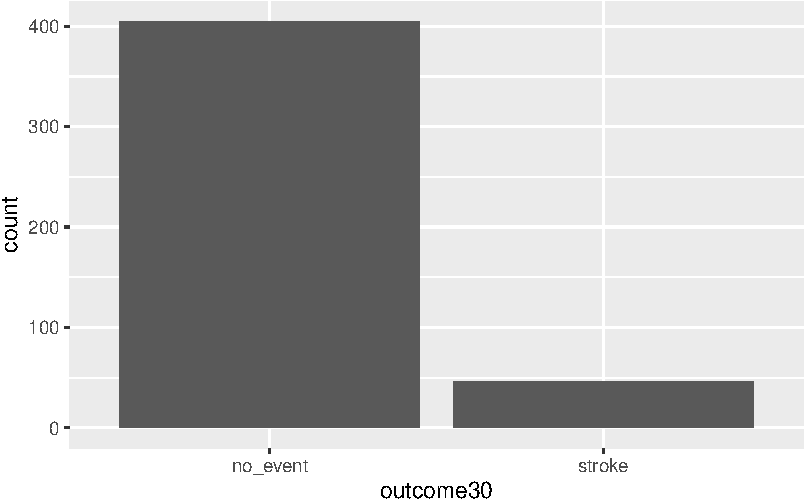
\includegraphics{Data-Case-Study_files/figure-pdf/fig-first-1.pdf}

}

\caption{\label{fig-first}Using \textbf{ggformula} to create a bar
chart.}

\end{figure}%

\begin{quote}
\textbf{Exercise}:\\
Explain Figure~\ref{fig-first}.
\end{quote}

This plot graphically shows us the total number of ``stroke'' and the
total number of ``no\_event''. However, this is not what we want. We
want to compare the 30-day outcomes for both treatment groups. So, we
need to break the data into different groups based on treatment type. In
the formula notation, we now update it to the form:

\begin{verbatim}
goal(y ~ x|z, data = MyData, ...) # pseudo-code for the formula template
\end{verbatim}

We read \texttt{y\ \textasciitilde{}\ x\textbar{}z} as ``y tilde x by
z'' and interpret it in the equivalent forms: ``y modeled by x for each
z''; ``y explained by x within each z''; or ``y accounted for by x
within z.'' For graphics, it's reasonable to read the formula as ``y
vs.~x for each z''. Figure Figure~\ref{fig-split} shows the results.

\begin{Shaded}
\begin{Highlighting}[]
\FunctionTok{gf\_bar}\NormalTok{(}\SpecialCharTok{\textasciitilde{}}\NormalTok{outcome30}\SpecialCharTok{|}\NormalTok{group, }\AttributeTok{data =}\NormalTok{ stent\_study) }
\end{Highlighting}
\end{Shaded}

\begin{figure}[H]

\centering{

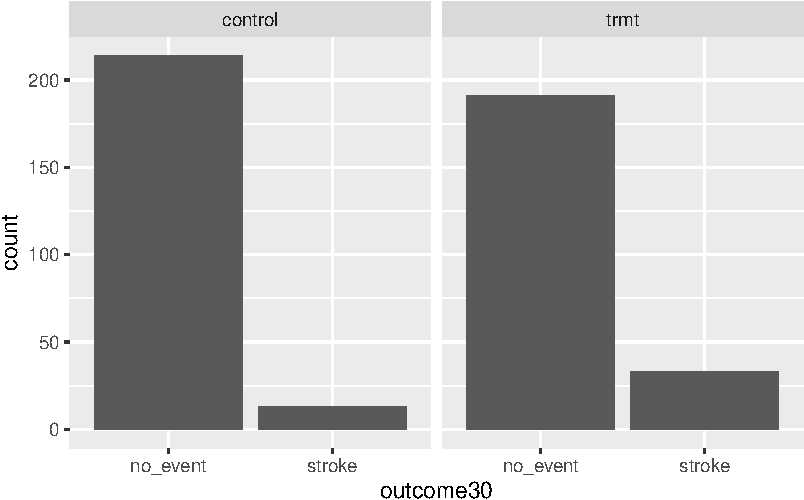
\includegraphics{Data-Case-Study_files/figure-pdf/fig-split-1.pdf}

}

\caption{\label{fig-split}Bar charts conditioned on the \texttt{group}
variable.}

\end{figure}%

\subsubsection{More advanced graphics}\label{more-advanced-graphics}

As a prelude for things to come, the above graphic needs work. The
labels don't help and there is no title. We could add color. Does it
make more sense to use proportions? Here is the code and results for a
better graph, see Figure Figure~\ref{fig-cs1}. Don't worry if this seems
a bit advanced, but feel free to examine each new component of this
code.

\begin{Shaded}
\begin{Highlighting}[]
\CommentTok{\# This code creates a graph showing the impact of stents on stroke.}
\CommentTok{\# The \textasciigrave{}gf\_props()\textasciigrave{} function creates a bar graph showing the number of events}
\CommentTok{\# for each experimental group. The \textasciigrave{}fill\textasciigrave{} argument specifies the fill color}
\CommentTok{\# for each group. The \textasciigrave{}position = \textquotesingle{}fill\textquotesingle{}\textasciigrave{} argument specifies that the bars}
\CommentTok{\# should be filled to the top.}

\CommentTok{\# The \textasciigrave{}gf\_labs()\textasciigrave{} function adds the title, subtitle, x{-}axis label, and y{-}axis}
\CommentTok{\# label to the graph.}

\CommentTok{\# The \textasciigrave{}gf\_theme()\textasciigrave{} function applies a black{-}and{-}white theme to the graph.}

\NormalTok{stent\_study }\SpecialCharTok{\%\textgreater{}\%}
\FunctionTok{gf\_props}\NormalTok{(}\SpecialCharTok{\textasciitilde{}}\NormalTok{group, }\AttributeTok{fill =} \SpecialCharTok{\textasciitilde{}}\NormalTok{outcome30, }\AttributeTok{position =} \StringTok{\textquotesingle{}fill\textquotesingle{}}\NormalTok{) }\SpecialCharTok{\%\textgreater{}\%}
  \FunctionTok{gf\_labs}\NormalTok{(}\AttributeTok{title =} \StringTok{"Impact of Stents of Stroke"}\NormalTok{,}
          \AttributeTok{subtitle =} \StringTok{\textquotesingle{}Experiment with 451 Patients\textquotesingle{}}\NormalTok{,}
          \AttributeTok{x =} \StringTok{"Experimental Group"}\NormalTok{,}
          \AttributeTok{y =} \StringTok{"Number of Events"}\NormalTok{) }\SpecialCharTok{\%\textgreater{}\%}
  \FunctionTok{gf\_theme}\NormalTok{(}\FunctionTok{theme\_bw}\NormalTok{())}
\end{Highlighting}
\end{Shaded}

\begin{figure}[H]

\centering{

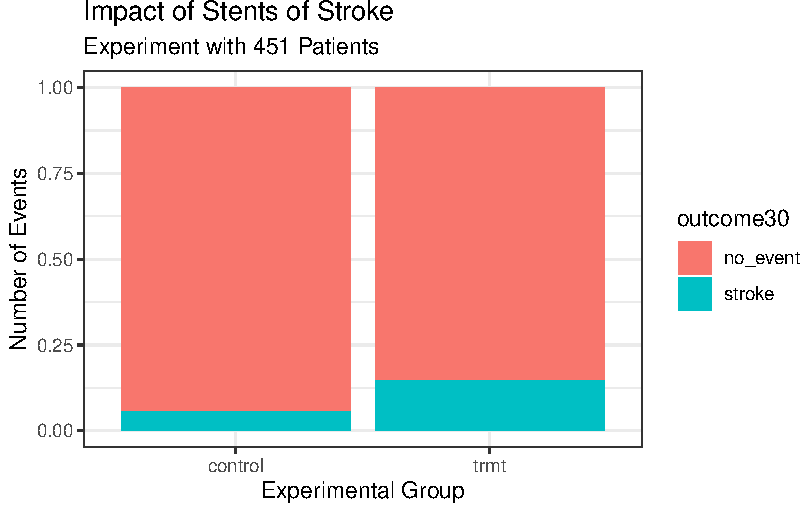
\includegraphics{Data-Case-Study_files/figure-pdf/fig-cs1-1.pdf}

}

\caption{\label{fig-cs1}Better graph.}

\end{figure}%

Notice that we used the pipe operator, \texttt{\%\textgreater{}\%}. This
operator allows us to string functions together in a manner that makes
it easier to read the code. In the above code, we are sending the data
object \texttt{stent\_study} into the function \texttt{gf\_props()} to
use as data, so we don't need the \texttt{data\ =} argument. In math,
this is a composition of functions. Instead of \texttt{f(g(x))} we could
use a pipe \texttt{f(g(x))\ =\ g(x)\ \%\textgreater{}\%\ f()}.

\subsection{Conclusion}\label{conclusion}

These two summary statistics (the proportions of people who had a
stroke) are useful in looking for differences in the groups, and we are
in for a surprise: an additional 9\% of patients in the treatment group
had a stroke! This is important for two reasons. First, it is contrary
to what doctors expected, which was that stents would \emph{reduce} the
rate of strokes. Second, it leads to a statistical question: do the data
show a real difference due to the treatment?

This second question is subtle. Suppose you flip a coin 100 times. While
the chance a coin lands heads in any given coin flip is 50\%, we
probably won't observe exactly 50 heads. This type of fluctuation is
part of almost any type of data generating process. It is possible that
the 9\% difference in the stent study is due to this natural variation.
However, the larger the difference we observe (for a particular sample
size), the less believable it is that the difference is due to chance.
So what we are really asking is the following: is the difference so
large that we should reject the notion that it was due to chance?

This is a preview of step 4, analyze the data, and step 5, form a
conclusion, of the analysis cycle. While we haven't yet covered
statistical tools to fully address these steps, we can comprehend the
conclusions of the published analysis: there was compelling evidence of
harm by stents in this study of stroke patients.

\textbf{Be careful:} Do not generalize the results of this study to all
patients and all stents. This study looked at patients with very
specific characteristics who volunteered to be a part of this study and
who may not be representative of all stroke patients. In addition, there
are many types of stents and this study only considered the
self-expanding Wingspan stent (Boston Scientific). However, this study
does leave us with an important lesson: we should keep our eyes open for
surprises.

\chapter{Data Basics}\label{sec-DB}

\section{Objectives}\label{objectives-2}

\begin{enumerate}
\def\labelenumi{\arabic{enumi})}
\item
  Differentiate between various statistical terminologies such as
  \emph{case, observational unit, variables, data frame, tidy data,
  numerical variable, discrete numeric variable, continuous numeric
  variable, categorical variable, levels, scatterplot, associated
  variables}, and \emph{independent}, and construct examples to
  demonstrate their proper use in context.
\item
  Within a given dataset, evaluate different types of variables and
  justify their classifications (e.g.~categorical, discrete numerical,
  continuous numerical).
\item
  Given a study description, develop an appropriate research question
  and justify the organization of data as tidy.
\item
  Create and interpret scatterplots using \texttt{R} to analyze the
  relationship between two numerical variables by evaluating the
  strength and direction of the association.
\end{enumerate}

\section{Data basics}\label{data-basics-1}

Effective presentation and description of data is a first step in most
analyses. This chapter introduces one structure for organizing data, as
well as some terminology that will be used throughout this book.

\subsection{Observations, variables, and data
matrices}\label{observations-variables-and-data-matrices}

For reference we will be using a data set concerning 50 emails received
in 2012. These observations will be referred to as the \texttt{email50}
data set, and they are a random sample from a larger data set. This data
is in the \textbf{openintro} package so let's install and then load this
package.

\begin{Shaded}
\begin{Highlighting}[]
\FunctionTok{install.packages}\NormalTok{(}\StringTok{"openintro"}\NormalTok{)}
\FunctionTok{library}\NormalTok{(openintro)}
\end{Highlighting}
\end{Shaded}

Table~\ref{tbl-db1} shows 4 rows of the \texttt{email50} data set and we
have elected to only list 5 variables for ease of observation.

Each row in the table represents a single email or \textbf{case}. A case
is also sometimes called a \textbf{unit of observation} or an
\textbf{observational unit}. The columns represent \textbf{variables},
which represent characteristics for each of the cases (emails). For
example, the first row represents email 1, which is not spam, contains
21,705 characters, 551 line breaks, is written in HTML format, and
contains only small numbers.

\begin{longtable}[]{@{}lrrll@{}}

\caption{\label{tbl-db1}First 5 rows of email data frame}

\tabularnewline

\toprule\noalign{}
spam & num\_char & line\_breaks & format & number \\
\midrule\noalign{}
\endhead
\bottomrule\noalign{}
\endlastfoot
0 & 21.705 & 551 & 1 & small \\
0 & 7.011 & 183 & 1 & big \\
1 & 0.631 & 28 & 0 & none \\
0 & 15.829 & 242 & 1 & small \\

\end{longtable}

Let's look at the first 10 rows of data from \texttt{email50} using
\texttt{R}. Remember to ask the two questions:

\emph{What do we want \texttt{R} to do?} and

\emph{What must we give \texttt{R} for it to do this?}

We want the first 10 rows so we use \texttt{head()} and \texttt{R} needs
the data object and the number of rows. The data object is called
\texttt{email50} and is accessible once the \textbf{openintro} package
is loaded.

\begin{Shaded}
\begin{Highlighting}[]
\FunctionTok{head}\NormalTok{(email50, }\AttributeTok{n =} \DecValTok{10}\NormalTok{)}
\end{Highlighting}
\end{Shaded}

\begin{verbatim}
# A tibble: 10 x 21
   spam  to_multiple from     cc sent_email time                image attach
   <fct> <fct>       <fct> <int> <fct>      <dttm>              <dbl>  <dbl>
 1 0     0           1         0 1          2012-01-04 13:19:16     0      0
 2 0     0           1         0 0          2012-02-16 20:10:06     0      0
 3 1     0           1         4 0          2012-01-04 15:36:23     0      2
 4 0     0           1         0 0          2012-01-04 17:49:52     0      0
 5 0     0           1         0 0          2012-01-27 09:34:45     0      0
 6 0     0           1         0 0          2012-01-17 17:31:57     0      0
 7 0     0           1         0 0          2012-03-18 04:18:55     0      0
 8 0     0           1         0 1          2012-03-31 13:58:56     0      0
 9 0     0           1         1 1          2012-01-11 01:57:54     0      0
10 0     0           1         0 0          2012-01-07 19:29:16     0      0
# i 13 more variables: dollar <dbl>, winner <fct>, inherit <dbl>, viagra <dbl>,
#   password <dbl>, num_char <dbl>, line_breaks <int>, format <fct>,
#   re_subj <fct>, exclaim_subj <dbl>, urgent_subj <fct>, exclaim_mess <dbl>,
#   number <fct>
\end{verbatim}

In practice, it is especially important to ask clarifying questions to
ensure important aspects of the data are understood. For instance, it is
always important to be sure we know what each variable means and the
units of measurement. Descriptions of all variables in the
\texttt{email50} data set are given in its documentation which can be
accessed in \texttt{R} by using the \texttt{?} command:

\begin{verbatim}
?email50
\end{verbatim}

(Note that not all data sets will have associated documentation; the
authors of \textbf{openintro} package included this documentation with
the \texttt{email50} data set contained in the package.)

The data in \texttt{email50} represent a \textbf{data matrix}, or in
\texttt{R} terminology a \textbf{data frame} or \textbf{tibble}
\footnote{A tibble is a data frame with attributes for such things as
  better display and printing.}, which is a common way to organize data.
Each row of a data matrix corresponds to a unique case, and each column
corresponds to a variable. This is called \textbf{tidy data}.\footnote{Tidy
  data is data in which each row corresponds to a unique case and each
  column represents a single variable. For more information on tidy
  data, see the \emph{Simply Statistics} blog and the \emph{R for Data
  Science} book by Hadley Wickham and Garrett Grolemund.} The data frame
for the stroke study introduced in the previous chapter had patients as
the cases and there were three variables recorded for each patient. If
we are thinking of patients as the unit of observation, then this data
is tidy.

\begin{verbatim}
# A tibble: 10 x 3
   group   outcome30 outcome365
   <chr>   <chr>     <chr>     
 1 control no_event  no_event  
 2 trmt    no_event  no_event  
 3 control no_event  no_event  
 4 trmt    no_event  no_event  
 5 trmt    no_event  no_event  
 6 control no_event  no_event  
 7 trmt    no_event  no_event  
 8 control no_event  no_event  
 9 control no_event  no_event  
10 control no_event  no_event  
\end{verbatim}

If we think of an outcome as a unit of observation, then it is not tidy
since the two outcome columns are variable values (month or year). The
tidy data for this case would be:

\begin{verbatim}
# A tibble: 10 x 4
   patient_id group   time  result  
        <int> <chr>   <chr> <chr>   
 1          1 control month no_event
 2          1 control year  no_event
 3          2 trmt    month no_event
 4          2 trmt    year  no_event
 5          3 control month no_event
 6          3 control year  no_event
 7          4 trmt    month no_event
 8          4 trmt    year  no_event
 9          5 trmt    month no_event
10          5 trmt    year  no_event
\end{verbatim}

There are three interrelated rules which make a data set tidy:

\begin{enumerate}
\def\labelenumi{\arabic{enumi}.}
\tightlist
\item
  Each variable must have its own column.\\
\item
  Each observation must have its own row.\\
\item
  Each value must have its own cell.
\end{enumerate}

Why ensure that your data is tidy? There are two main advantages:

\begin{enumerate}
\def\labelenumi{\arabic{enumi}.}
\item
  There's a general advantage to picking one consistent way of storing
  data. If you have a consistent data structure, it's easier to learn
  the tools that work with it because they have an underlying
  uniformity.
\item
  There's a specific advantage to placing variables in columns because
  it allows \texttt{R}'s vectorized nature to shine. This will be more
  clear as we progress in our studies. Since most built-in \texttt{R}
  functions work with vectors of values, it makes transforming tidy data
  feel particularly natural.
\end{enumerate}

Data frames are a convenient way to record and store data. If another
individual or case is added to the data set, an additional row can be
easily added. Similarly, another column can be added for a new variable.

\begin{quote}
\textbf{Exercise}:\\
We consider a publicly available data set that summarizes information
about the 3,142 counties in the United States, and we create a data set
called \texttt{county\_subset} data set. This data set will include
information about each county: its name, the state where it resides, its
population in 2000 and 2010, per capita federal spending, poverty rate,
and four additional characteristics. We create this data object in the
code following this description. The parent data set is part of the
\texttt{usdata} library and is called \texttt{county\_complete}. The
variables are summarized in the help menu built into the \textbf{usdata}
package\footnote{\href{http://quickfacts.census.gov/qfd/index.html}{These
  data were collected from the US Census website.}}. How might these
data be organized in a data matrix? \footnote{Each county may be viewed
  as a case, and there are ten pieces of information recorded for each
  case. A table with 3,142 rows and 10 columns could hold these data,
  where each row represents a county and each column represents a
  particular piece of information.}
\end{quote}

Using \texttt{R} we will create our data object. First we load the
library \texttt{usdata}.

\begin{Shaded}
\begin{Highlighting}[]
\FunctionTok{library}\NormalTok{(usdata)}
\end{Highlighting}
\end{Shaded}

We only want a subset of the columns and we will use the \texttt{select}
verb in \texttt{dplyr} to select and rename columns. We also create a
new variable which is federal spending per capita using the
\texttt{mutate} function.

\begin{Shaded}
\begin{Highlighting}[]
\NormalTok{county\_subset }\OtherTok{\textless{}{-}}\NormalTok{ county\_complete }\SpecialCharTok{\%\textgreater{}\%} 
  \FunctionTok{select}\NormalTok{(name, state, pop2000, pop2010, }\AttributeTok{fed\_spend =}\NormalTok{ fed\_spending\_2009, }
         \AttributeTok{poverty =}\NormalTok{ poverty\_2010, }\AttributeTok{homeownership =}\NormalTok{ homeownership\_2010, }
         \AttributeTok{multi\_unit =}\NormalTok{ housing\_multi\_unit\_2010, }\AttributeTok{income =}\NormalTok{ per\_capita\_income\_2010, }
         \AttributeTok{med\_income =}\NormalTok{ median\_household\_income\_2010) }\SpecialCharTok{\%\textgreater{}\%}
  \FunctionTok{mutate}\NormalTok{(}\AttributeTok{fed\_spend =}\NormalTok{ fed\_spend }\SpecialCharTok{/}\NormalTok{ pop2010)}
\end{Highlighting}
\end{Shaded}

Using \texttt{R}, we will display seven rows of the
\texttt{county\_subset} data frame.

\begin{Shaded}
\begin{Highlighting}[]
\FunctionTok{head}\NormalTok{(county\_subset, }\AttributeTok{n =} \DecValTok{7}\NormalTok{)}
\end{Highlighting}
\end{Shaded}

\begin{verbatim}
            name   state pop2000 pop2010 fed_spend poverty homeownership
1 Autauga County Alabama   43671   54571  6.068095    10.6          77.5
2 Baldwin County Alabama  140415  182265  6.139862    12.2          76.7
3 Barbour County Alabama   29038   27457  8.752158    25.0          68.0
4    Bibb County Alabama   20826   22915  7.122016    12.6          82.9
5  Blount County Alabama   51024   57322  5.130910    13.4          82.0
6 Bullock County Alabama   11714   10914  9.973062    25.3          76.9
7  Butler County Alabama   21399   20947  9.311835    25.0          69.0
  multi_unit income med_income
1        7.2  24568      53255
2       22.6  26469      50147
3       11.1  15875      33219
4        6.6  19918      41770
5        3.7  21070      45549
6        9.9  20289      31602
7       13.7  16916      30659
\end{verbatim}

\subsection{Types of variables}\label{types-of-variables}

Examine the \texttt{fed\_spend}, \texttt{pop2010}, and \texttt{state}
variables in the \texttt{county} data set. Each of these variables is
inherently different from the others, yet many of them share certain
characteristics.

First consider \texttt{fed\_spend}. It is said to be a \textbf{numerical
variable} (sometimes called a quantitative variable) since it can take a
wide range of numerical values, and it is sensible to add, subtract, or
take averages with those values. On the other hand, we would not
classify a variable reporting telephone area codes as numerical; even
though area codes are made up of numerical digits, their average, sum,
and difference have no clear meaning.

The \texttt{pop2010} variable is also numerical; it is sensible to add,
subtract, or take averages with those values, although it seems to be a
little different than \texttt{fed\_spend}. This variable of the
population count can only be a whole non-negative number (\(0\), \(1\),
\(2\), \(...\)). For this reason, the population variable is said to be
\textbf{discrete} since it can only take specific numerical values. On
the other hand, the federal spending variable is said to be
\textbf{continuous} because it can take on any value in some interval.
Now technically, there are no truly continuous numerical variables since
all measurements are finite up to some level of accuracy or measurement
precision (e.g., we typically measure federal spending in dollars and
cents). However, in this book, we will treat both types of numerical
variables the same, that is as continuous variables for statistical
modeling. The only place this will be different in this book is in
probability models, which we will see in the probability modeling block.

The variable \texttt{state} can take up to 51 values, after accounting
for Washington, DC, and are summarized as: \emph{Alabama},
\emph{Alaska}, \ldots, and \emph{Wyoming}. Because the responses
themselves are categories, \texttt{state} is a \textbf{categorical
variable} (sometimes also called a qualitative variable), and the
possible values are called the variable's \textbf{levels}.

\begin{figure}

\centering{

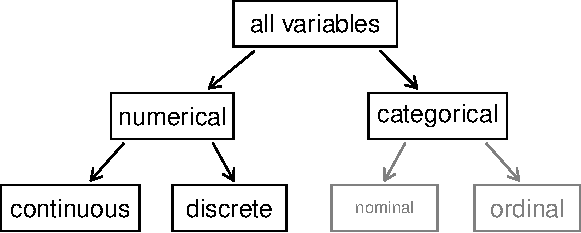
\includegraphics{Data-Basics_files/figure-pdf/fig-tax-1.pdf}

}

\caption{\label{fig-tax}Taxonomy of Variables.}

\end{figure}%

Finally, consider a hypothetical variable on education, which describes
the highest level of education completed and takes on one of the values
\emph{noHS}, \emph{HS}, \emph{College} or \emph{Graduate\_school}. This
variable seems to be a hybrid: it is a categorical variable but the
levels have a natural ordering. A variable with these properties is
called an \textbf{ordinal} variable. A categorical variable with levels
that do not have a natural ordering is called a \textbf{nominal}
variable. To simplify analyses, any ordinal variables in this book will
be treated as nominal categorical variables. In \texttt{R}, categorical
variables can be treated in different ways; one of the key differences
is that we can leave them as character values (character strings, or
text) or as factors. A factor is essentially a categorical variable with
defined \emph{levels}. When \texttt{R} handles factors, it is only
concerned about the \emph{levels} of the factors. We will learn more
about this as we progress.

Figure~\ref{fig-tax} captures this classification of variables we have
described.

\begin{quote}
\textbf{Exercise}:\\
Data were collected about students in a statistics course. Three
variables were recorded for each student: number of siblings, student
height, and whether the student had previously taken a statistics
course. Classify each of the variables as continuous numerical, discrete
numerical, or categorical.\footnote{The number of siblings and student
  height represent numerical variables. Because the number of siblings
  is a count, it is discrete. Height varies continuously, so it is a
  continuous numerical variable. The last variable classifies students
  into two categories -- those who have and those who have not taken a
  statistics course -- which makes this variable categorical.}
\end{quote}

\begin{quote}
\textbf{Exercise}:\\
Consider the variables \texttt{group} and \texttt{outcome30} from the
stent study in the case study chapter. Are these numerical or
categorical variables? \footnote{There are only two possible values for
  each variable, and in both cases they describe categories. Thus, each
  is a categorical variable.}
\end{quote}

\subsection{Relationships between
variables}\label{relationships-between-variables}

Many analyses are motivated by a researcher looking for a relationship
between two or more variables. This is the heart of statistical
modeling. A social scientist may like to answer some of the following
questions:

\begin{enumerate}
\def\labelenumi{\arabic{enumi}.}
\tightlist
\item
  Is federal spending, on average, higher or lower in counties with high
  rates of poverty?\\
\item
  If homeownership is lower than the national average in one county,
  will the percent of multi-unit structures in that county likely be
  above or below the national average?
\end{enumerate}

These are what statisticians refer to as \textbf{research questions},
specific and measurable questions that guide the data collection and
analysis process. To answer these questions, data must be collected,
such as the \texttt{county\_complete} data set. Examining summary
statistics could provide insights for each of the two questions about
counties. Graphs can be used to visually summarize data and are useful
for answering such questions as well.

\textbf{Scatterplots} are one type of graph used to study the
relationship between two numerical variables. Figure~\ref{fig-pov1}
compares the variables \texttt{fed\_spend} and \texttt{poverty}. Each
point on the plot represents a single county. For instance, the
highlighted dot corresponds to County 1088 in the
\texttt{county\_subset} data set: Owsley County, Kentucky, which had a
poverty rate of 41.5\% and federal spending of \$21.50 per capita. The
dense cloud in the scatterplot suggests a relationship between the two
variables: counties with a high poverty rate also tend to have slightly
more federal spending. We might brainstorm as to why this relationship
exists and investigate each idea to determine which is the most
reasonable explanation.

\begin{figure}

\centering{

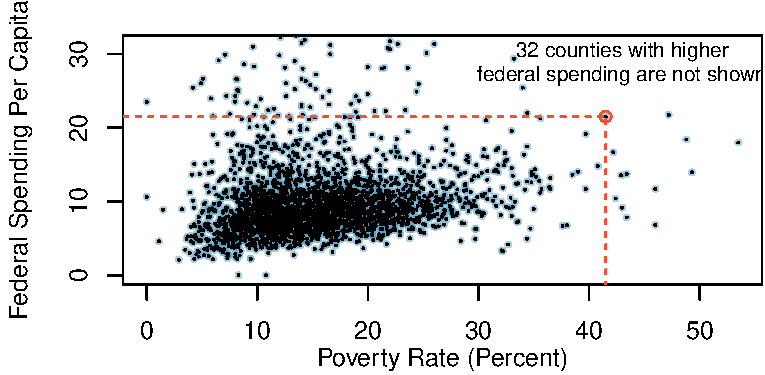
\includegraphics{Data-Basics_files/figure-pdf/fig-pov1-1.pdf}

}

\caption{\label{fig-pov1}A scatterplot showing fed\_spend against
poverty. Owsley County of Kentucky, with a poverty rate of 41.5\% and
federal spending of \$21.50 per capita, is highlighted.}

\end{figure}%

\begin{quote}
\textbf{Exercise}:\\
Examine the variables in the \texttt{email50} data set. Create two
research questions about the relationships between these variables that
are of interest to you.\footnote{Two sample questions: (1) Intuition
  suggests that if there are many line breaks in an email then there
  would also tend to be many characters: does this hold true? (2) Is
  there a connection between whether an email format is plain text
  (versus HTML) and whether it is a spam message?}
\end{quote}

The \texttt{fed\_spend} and \texttt{poverty} variables are said to be
associated because the plot shows a discernible pattern. When two
variables show some connection with one another, they are called
\textbf{associated variables}. Associated variables can also be called
\textbf{dependent} variables and vice-versa.

\begin{quote}
\emph{Example}:\\
The relationship between the homeownership rate and the percent of units
in multi-unit structures (e.g.~apartments, condos) is visualized using a
scatterplot in Figure~\ref{fig-homeown}. Are these variables associated?
\end{quote}

It appears that the larger the fraction of units in multi-unit
structures, the lower the homeownership rate. Since there is some
relationship between the variables, they are associated.

\begin{figure}

\centering{

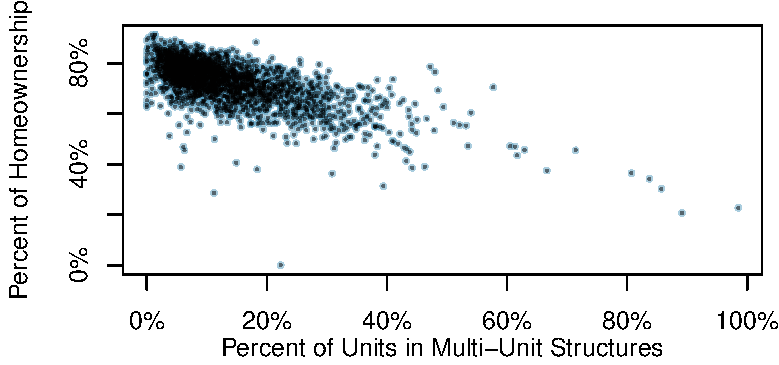
\includegraphics{Data-Basics_files/figure-pdf/fig-homeown-1.pdf}

}

\caption{\label{fig-homeown}A scatterplot of the homeownership rate
versus the percent of units that are in multi-unit structures for all
3,143 counties.}

\end{figure}%

Because there is a downward trend in Figure~\ref{fig-homeown} --
counties with more units in multi-unit structures are associated with
lower homeownership -- these variables are said to be \textbf{negatively
associated}. A \textbf{positive association} (upward trend) is shown in
the relationship between the \texttt{poverty} and \texttt{fed\_spend}
variables represented in Figure~\ref{fig-pov1}, where counties with
higher poverty rates tend to receive more federal spending per capita.

If two variables are not associated, then they are said to be
\textbf{independent}. That is, two variables are independent if there is
no evident relationship between the two.

\begin{quote}
A pair of variables are either related in some way (associated) or not
(independent). No pair of variables is both associated and independent.
\end{quote}

\subsection{Creating a scatterplot}\label{creating-a-scatterplot}

In this section, we will create a simple scatterplot and then ask you to
create one on your own. First, we will recreate the scatterplot seen in
Figure~\ref{fig-pov1}. This figure uses the \texttt{county\_subset} data
set.

Here are two questions:

\emph{What do we want \texttt{R} to do?} and

\emph{What must we give \texttt{R} for it to do this?}

We want \texttt{R} to create a scatterplot and to do this it needs, at a
minimum, the data object, what we want on the \(x\)-axis, and what we
want on the \(y\)-axis. More information on
\href{https://cran.r-project.org/web/packages/ggformula/vignettes/ggformula.html}{\textbf{ggformula}}
can be found
\href{https://cran.r-project.org/web/packages/ggformula/vignettes/ggformula-blog.html}{here}.

\begin{Shaded}
\begin{Highlighting}[]
\NormalTok{county\_subset }\SpecialCharTok{\%\textgreater{}\%}
  \FunctionTok{gf\_point}\NormalTok{(fed\_spend }\SpecialCharTok{\textasciitilde{}}\NormalTok{ poverty)}
\end{Highlighting}
\end{Shaded}

\begin{figure}[H]

\centering{

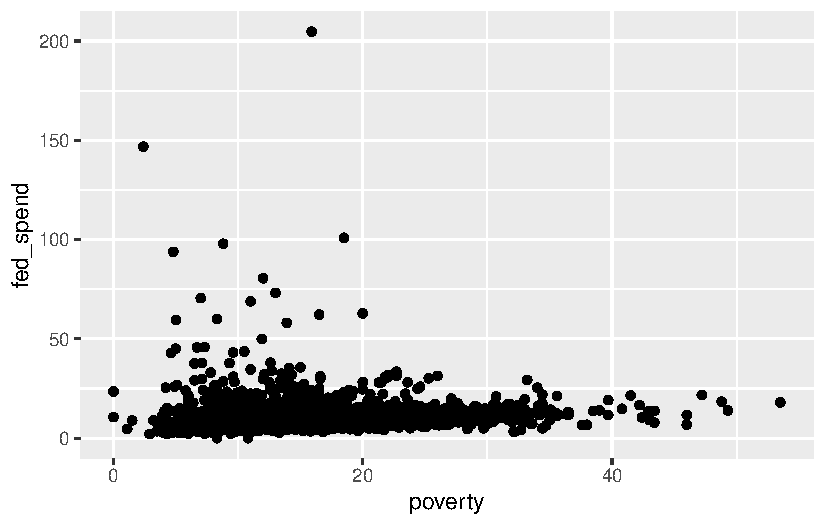
\includegraphics{Data-Basics_files/figure-pdf/fig-pov2-1.pdf}

}

\caption{\label{fig-pov2}Scatterplot with \textbf{ggformula}.}

\end{figure}%

Figure~\ref{fig-pov2} is bad. There are poor axis labels, no title,
dense clustering of points, and the \(y\)-axis is being driven by a
couple of extreme points. We will need to clear this up. Again, try to
read the code and use \texttt{help()} or \texttt{?} to determine the
purpose of each command in Figure~\ref{fig-pov3}.

\begin{Shaded}
\begin{Highlighting}[]
\NormalTok{county\_subset }\SpecialCharTok{\%\textgreater{}\%}
  \FunctionTok{filter}\NormalTok{(fed\_spend }\SpecialCharTok{\textless{}} \DecValTok{32}\NormalTok{) }\SpecialCharTok{\%\textgreater{}\%}
  \FunctionTok{gf\_point}\NormalTok{(fed\_spend }\SpecialCharTok{\textasciitilde{}}\NormalTok{ poverty,}
           \AttributeTok{xlab =} \StringTok{"Poverty Rate (Percent)"}\NormalTok{, }
           \AttributeTok{ylab =} \StringTok{"Federal Spending Per Capita"}\NormalTok{,}
           \AttributeTok{title =} \StringTok{"A scatterplot showing fed\_spend against poverty"}\NormalTok{, }
           \AttributeTok{cex =} \DecValTok{1}\NormalTok{, }\AttributeTok{alpha =} \FloatTok{0.2}\NormalTok{) }\SpecialCharTok{\%\textgreater{}\%}
  \FunctionTok{gf\_theme}\NormalTok{(}\FunctionTok{theme\_classic}\NormalTok{())}
\end{Highlighting}
\end{Shaded}

\begin{figure}[H]

\centering{

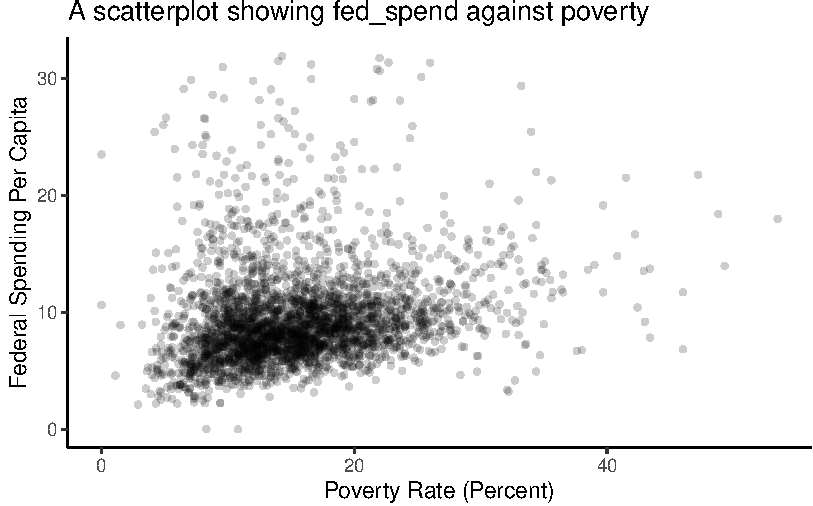
\includegraphics{Data-Basics_files/figure-pdf/fig-pov3-1.pdf}

}

\caption{\label{fig-pov3}Better example of a scatterplot.}

\end{figure}%

\begin{quote}
\textbf{Exercise}:\\
Create the scatterplot in Figure~\ref{fig-homeown}.
\end{quote}

\chapter{Overview of Data Collection Principles}\label{sec-ODCP}

\section{Objectives}\label{objectives-3}

\begin{enumerate}
\def\labelenumi{\arabic{enumi})}
\item
  Differentiate between various statistical terminologies such as
  \emph{population, sample, anecdotal evidence, bias, simple random
  sample, systematic sample, representative sample, non-response bias,
  convenience sample, explanatory variable,} \emph{response variable,
  observational study, cohort, experiment, randomized experiment,} and
  \emph{placebo}, and construct examples to demonstrate their proper use
  in context.
\item
  Evaluate descriptions of research project to identify the population
  of interest, assess the generalizability of the study, determine the
  explanatory and response variables, classify the study as
  observational or experimental, and determine the type of sample used.
\item
  Design and justify sampling procedures for various research contexts,
  comparing the strengths and weaknesses of different sampling methods
  (simple random, systematic, convenience, etc.) and proposing
  improvements to minimize bias and enhance representativeness.
\end{enumerate}

\section{Overview of data collection
principles}\label{overview-of-data-collection-principles-1}

The first step in conducting research is to identify topics or questions
that are to be investigated. A clearly laid out research question is
helpful in identifying what subjects or cases should be studied and what
variables are important. It is also important to consider \emph{how}
data are collected so that they are reliable and help achieve the
research goals.

\subsection{Populations and samples}\label{populations-and-samples}

Consider the following three research questions:

\begin{enumerate}
\def\labelenumi{\arabic{enumi}.}
\tightlist
\item
  What is the average mercury content in swordfish in the Atlantic
  Ocean?\\
\item
  Over the last 5 years, what is the average time to complete a degree
  for Duke undergraduate students?\\
\item
  Does a new drug reduce the number of deaths in patients with severe
  heart disease?
\end{enumerate}

Each research question refers to a target \textbf{population}, the
entire collection of individuals about which we want information. In the
first question, the target population is all swordfish in the Atlantic
Ocean, and each fish represents a case. It is usually too expensive to
collect data for every case in a population. Instead, a sample is taken.
A \textbf{sample} represents a subset of the cases and is often a small
fraction of the population. For instance, 60 swordfish (or some other
number) in the population might be selected, and this sample data may be
used to provide an estimate of the population average and answer the
research question.

\begin{quote}
\textbf{Exercise}:\\
For the second and third questions above, identify the target population
and what represents an individual case.\footnote{2) Notice that the
  second question is only relevant to students who complete their
  degree; the average cannot be computed using a student who never
  finished her degree. Thus, only Duke undergraduate students who have
  graduated in the last five years represent cases in the population
  under consideration. Each such student would represent an individual
  case. 3) A person with severe heart disease represents a case. The
  population includes all people with severe heart disease.}
\end{quote}

\subsection{Anecdotal evidence}\label{anecdotal-evidence}

Consider the following possible responses to the three research
questions:

\begin{enumerate}
\def\labelenumi{\arabic{enumi}.}
\tightlist
\item
  A man on the news got mercury poisoning from eating swordfish, so the
  average mercury concentration in swordfish must be dangerously high.
\item
  I met two students who took more than 7 years to graduate from Duke,
  so it must take longer to graduate at Duke than at many other
  colleges.
\item
  My friend's dad had a heart attack and died after they gave him a new
  heart disease drug, so the drug must not work.
\end{enumerate}

Each conclusion is based on data. However, there are two problems.
First, the data only represent one or two cases. Second, and more
importantly, it is unclear whether these cases are actually
representative of the population. Data collected in this haphazard
fashion are called \textbf{anecdotal evidence}.

\begin{figure}[H]

{\centering 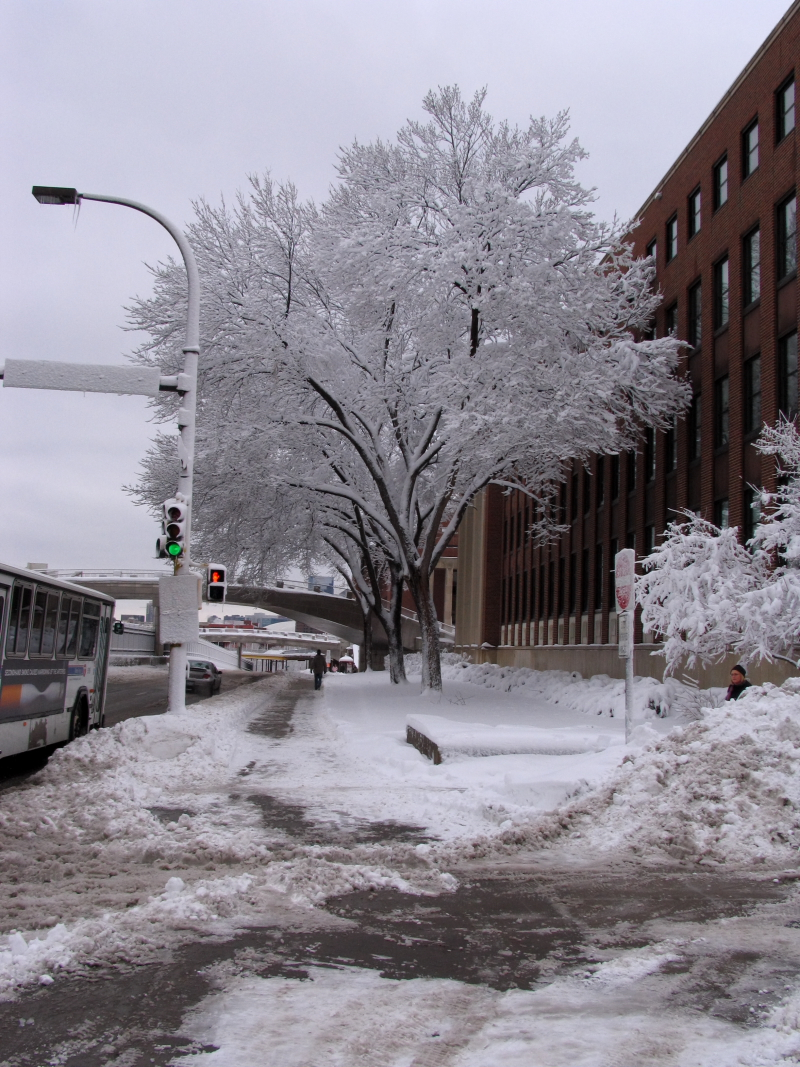
\includegraphics{./figures/mnWinter.JPG}

}

\caption{In February 2010, some media pundits cited one large snow storm
as evidence against global warming. As comedian Jon Stewart pointed out,
\emph{It's one storm, in one region, of one country.}}

\end{figure}%

\begin{quote}
\textbf{Anecdotal evidence}: Be careful of data collected haphazardly.
Such evidence may be true and verifiable, but it may only represent
extraordinary cases.
\end{quote}

Anecdotal evidence typically is composed of unusual cases that we recall
based on their striking characteristics. For instance, we are more
likely to remember the two people we met who took 7 years to graduate
than the six others who graduated in four years. Instead of looking at
the most unusual cases, we should examine a sample of many cases that
represent the population.

\subsection{Sampling from a
population}\label{sampling-from-a-population}

We might try to estimate the time to graduation for Duke undergraduates
in the last 5 years by collecting a sample of students. All graduates in
the last 5 years represent the \emph{population}, and graduates who are
selected for review are collectively called the \emph{sample}. In
general, we always seek to \emph{randomly} select a sample from a
population. The most basic type of random selection is equivalent to how
raffles are conducted. For example, in selecting graduates, we could
write each graduate's name on a raffle ticket and draw 100 tickets. The
selected names would represent a random sample of 100 graduates. This is
illustrated in Figure~\ref{fig-randsamp} .

\begin{figure}

\centering{

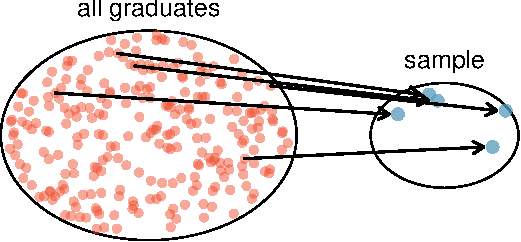
\includegraphics{Overview-of-Data-Collection-Principles_files/figure-pdf/fig-randsamp-1.pdf}

}

\caption{\label{fig-randsamp}In this graphic, five graduates are
randomly selected from the population to be included in the sample.}

\end{figure}%

Why pick a sample randomly? Why not just pick a sample by hand? Consider
the following scenario.

\begin{quote}
\textbf{Example}:\\
Suppose we ask a student who happens to be majoring in nutrition to
select several graduates for the study. What kind of students do you
think she might collect? Do you think her sample would be representative
of all graduates? \footnote{Perhaps she would pick a disproportionate
  number of graduates from health-related fields. Or perhaps her
  selection would be well-representative of the population. When
  selecting samples by hand, we run the risk of picking a \emph{biased}
  sample, even if that bias is unintentional or difficult to discern.}
\end{quote}

\begin{figure}

\centering{

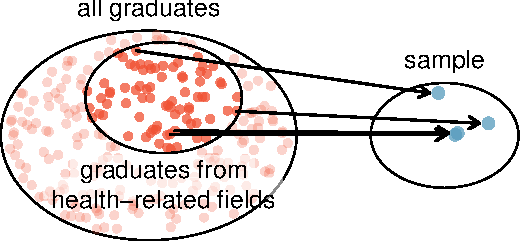
\includegraphics{Overview-of-Data-Collection-Principles_files/figure-pdf/fig-biased-1.pdf}

}

\caption{\label{fig-biased}Instead of sampling from all graduates
equally, a nutrition major might inadvertently pick graduates with
health-related majors disproportionately often.}

\end{figure}%

If someone was permitted to pick and choose exactly which graduates were
included in the sample, it is entirely possible that the sample could be
skewed to that person's interests, which may be entirely unintentional.
This introduces \textbf{sampling bias} (see Figure~\ref{fig-biased}),
where some individuals in the population are more likely to be sampled
than others. Sampling randomly helps resolve this problem. The most
basic random sample is called a \textbf{simple random sample}, which is
equivalent to using a raffle to select cases. This means that each case
in the population has an equal chance of being included and there is no
implied connection between the cases in the sample.

Sometimes a simple random sample is difficult to implement and an
alternative method is helpful. One such substitute is a
\textbf{systematic sample}, where one case is sampled after letting a
fixed number of others, say 10 other cases, pass by. Since this approach
uses a mechanism that is not easily subject to personal biases, it often
yields a reasonably representative sample. This book will focus on
simple random samples since the use of systematic samples is uncommon
and requires additional considerations of the context.

The act of taking a simple random sample helps minimize bias. However,
bias can crop up in other ways. Even when people are picked at random,
e.g.~for surveys, caution must be exercised if the non-response is high.
For instance, if only 30\% of the people randomly sampled for a survey
actually respond, and it is unclear whether the respondents are
\textbf{representative}\footnote{A representative sample accurately
  reflects the characteristics of the population.} of the entire
population, the survey might suffer from \textbf{non-response
bias}\footnote{Non-response bias is bias that can be introduced when
  subjects elect not to participate in a study. Often, the individuals
  that do participate are systematically different from the individuals
  who do not.}.

\begin{figure}

\centering{

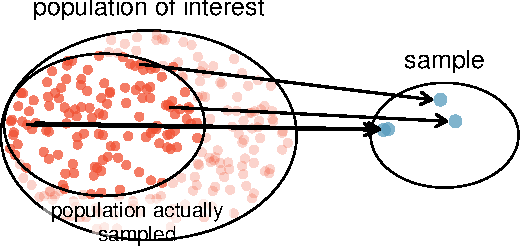
\includegraphics{Overview-of-Data-Collection-Principles_files/figure-pdf/fig-convsamp-1.pdf}

}

\caption{\label{fig-convsamp}Due to the possibility of non-response,
surveys studies may only reach a certain group within the population. It
is difficult, and often impossible, to completely fix this problem.}

\end{figure}%

Another common pitfall is a \textbf{convenience sample}, where
individuals who are easily accessible are more likely to be included in
the sample, see Figure~\ref{fig-convsamp}. For instance, if a political
survey is done by stopping people walking in the Bronx, it will not
represent all of New York City. It is often difficult to discern what
sub-population a convenience sample represents.

\begin{quote}
\textbf{Exercise}:\\
We can easily access ratings for products, sellers, and companies
through websites. These ratings are based only on those people who go
out of their way to provide a rating. If 50\% of online reviews for a
product are negative, do you think this means that 50\% of buyers are
dissatisfied with the product?\footnote{Answers will vary. From our own
  anecdotal experiences, we believe people tend to rant more about
  products that fell below expectations than rave about those that
  perform as expected. For this reason, we suspect there is a negative
  bias in product ratings on sites like Amazon. However, since our
  experiences may not be representative, we also keep an open mind.}
\end{quote}

\subsection{Explanatory and response
variables}\label{explanatory-and-response-variables}

Consider the following question for the \texttt{county} data set:

Is federal spending, on average, higher or lower in counties with high
rates of poverty?

If we suspect poverty might affect spending in a county, then poverty is
the \textbf{explanatory} variable and federal spending is the
\textbf{response} variable in the relationship.\footnote{Sometimes the
  explanatory variable is called the \textbf{independent} variable and
  the response variable is called the \textbf{dependent} variable.
  However, this becomes confusing since a \emph{pair} of variables might
  be independent or dependent, so be careful and consider the context
  when using or reading these words.} If there are many variables, it
may be possible to consider a number of them as explanatory variables.

\begin{quote}
\textbf{Explanatory} and \textbf{response} variables\\
To identify the explanatory variable in a pair of variables, identify
which of the two variables is suspected as explaining or causing changes
in the other. In data sets with more than two variables, it is possible
to have multiple explanatory variables. The response variable is the
outcome or result of interest.
\end{quote}

\begin{quote}
\textbf{Caution}: Association does not imply causation. Labeling
variables as \emph{explanatory} and \emph{response} does not guarantee
the relationship between the two is actually causal, even if there is an
association identified between the two variables. We use these labels
only to keep track of which variable we suspect affects the other. We
also use this language to help in our use of \texttt{R} and the formula
notation.
\end{quote}

In some cases, there is no explanatory or response variable. Consider
the following question:

If homeownership in a particular county is lower than the national
average, will the percent of multi-unit structures in that county likely
be above or below the national average?

It is difficult to decide which of these variables should be considered
the explanatory and response variable; i.e.~the direction is ambiguous,
so no explanatory or response labels are suggested here.

\subsection{Introducing observational studies and
experiments}\label{introducing-observational-studies-and-experiments}

There are two primary types of data collection: observational studies
and experiments.

Researchers perform an \textbf{observational study} when they collect
data in a way that does not directly interfere with how the data arise.
For instance, researchers may collect information via surveys, review
medical or company records, or follow a \textbf{cohort}\footnote{A
  cohort is a group of individuals who are similar in some way.} of many
similar individuals to study why certain diseases might develop. In each
of these situations, researchers merely observe what happens. In
general, observational studies can provide evidence of a naturally
occurring association between variables, but by themselves, they cannot
show a causal connection.

When researchers want to investigate the possibility of a causal
connection, they conduct an \textbf{experiment}, a study in which the
explanatory variables are assigned rather than observed. For instance,
we may suspect administering a drug will reduce mortality in heart
attack patients over the following year. To check if there really is a
causal connection between the explanatory variable and the response,
researchers will collect a sample of individuals and split them into
groups. The individuals in each group are \emph{assigned} a treatment.
When individuals are \emph{randomly} assigned to a treatment group, and
we are \emph{comparing} at least two treatments, the experiment is
called a \textbf{randomized comparative experiment}. For example, each
heart attack patient in the drug trial could be randomly assigned,
perhaps by flipping a coin, into one of two groups: the first group
receives a \textbf{placebo} (fake treatment) and the second group
receives the drug. The case study at the beginning of the book is
another example of an experiment, though that study did not employ a
placebo. Math 359 is a course on the design and analysis of experimental
data, DOE, at USAFA. In the Air Force, these types of experiments are an
important part of test and evaluation. Many Air Force analysts are
expert practitioners of DOE. In this book though, we will minimize our
discussion of DOE.

\begin{quote}
\textbf{Association} \(\neq\) \textbf{Causation}\\
Again, association does not imply causation. In a data analysis,
association does not imply causation, and causation can only be inferred
from a randomized experiment. Although, a hot field is the analysis of
causal relationships in observational data. This is important because
consider cigarette smoking, how do we know it causes lung cancer? We
only have observational data and clearly cannot do an experiment. We
think analysts will be charged in the near future with using causal
reasoning on observational data.
\end{quote}

\chapter{Studies}\label{sec-STUDY}

\section{Objectives}\label{objectives-4}

\begin{enumerate}
\def\labelenumi{\arabic{enumi})}
\item
  Differentiate between various statistical terminologies such as
  \emph{observational study, confounding variable, prospective study,
  retrospective study, simple random sampling, stratified sampling,
  strata, cluster sampling, multistage sampling, experiment, randomized
  experiment, control, replicate, blocking, treatment group, control
  group, blinded study, placebo, placebo effect,} and
  \emph{double-blind}, and construct examples to demonstrate their
  proper use in context.
\item
  Evaluate study descriptions using appropriate terminology, and analyze
  the study design for potential biases or confounding variables.
\item
  Given a scenario, identify and assess flaws in reasoning, and propose
  robust study and sampling methodologies to address these flaws.
\end{enumerate}

\section{Observational studies, sampling strategies, and
experiments}\label{observational-studies-sampling-strategies-and-experiments}

\subsection{Observational studies}\label{observational-studies}

Generally, data in \textbf{observational studies} are collected only by
monitoring what occurs, while experiments require the primary
explanatory variable in a study be assigned for each subject by the
researchers.

Making causal conclusions based on experiments is often reasonable.
However, making the same causal conclusions based on observational data
can be treacherous and is not recommended. Thus, observational studies
are generally only sufficient to show associations.

\begin{quote}
\textbf{Exercise}:\\
Suppose an observational study tracked sunscreen use and skin cancer,
and it was found that the more sunscreen someone used, the more likely
the person was to have skin cancer. Does this mean sunscreen
\emph{causes} skin cancer?\footnote{No.~See the paragraph following the
  exercise for an explanation.}
\end{quote}

Some previous research\footnote{http://www.sciencedirect.com/science/article/pii/S0140673698121682\\
  http://archderm.ama-assn.org/cgi/content/abstract/122/5/537\\
  Study with a similar scenario to that described here:\\
  http://onlinelibrary.wiley.com/doi/10.1002/ijc.22745/full} tells us
that using sunscreen actually reduces skin cancer risk, so maybe there
is another variable that can explain this hypothetical association
between sunscreen usage and skin cancer. One important piece of
information that is absent is sun exposure. If someone is out in the sun
all day, she is more likely to use sunscreen \emph{and} more likely to
get skin cancer. Exposure to the sun is unaccounted for in the simple
investigation.

\begin{figure}

\centering{

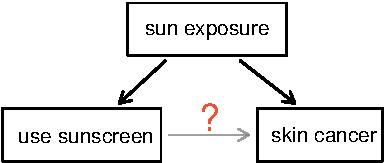
\includegraphics{Studies_files/figure-pdf/fig-confound-1.pdf}

}

\caption{\label{fig-confound}un exposure is a confounding variable
because it is related to both response and explanatory variables.}

\end{figure}%

Sun exposure is what is called a \textbf{confounding
variable},\footnote{Also called a \textbf{lurking variable},
  \textbf{confounding factor}, or a \textbf{confounder}.} which is a
variable that is correlated with both the explanatory and response
variables, see Figure~\ref{fig-confound}. While one method to justify
making causal conclusions from observational studies is to exhaust the
search for confounding variables, there is no guarantee that all
confounding variables can be examined or measured.

Let's look at an example of confounding visually. Using the \texttt{SAT}
data from the \textbf{mosaic} package let's look at expenditure per
pupil versus SAT scores. Figure~\ref{fig-confound2} is a plot of the
data.

\begin{quote}
\textbf{Exercise}:\\
What conclusion do you reach from the plot in
Figure~\ref{fig-confound2}?\footnote{It appears that average SAT score
  declines as expenditures per student increases.}
\end{quote}

\begin{figure}

\centering{

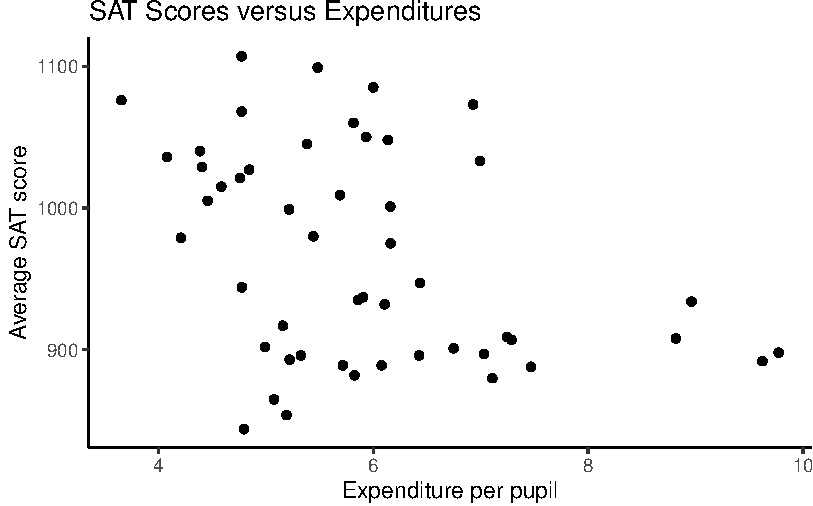
\includegraphics{Studies_files/figure-pdf/fig-confound2-1.pdf}

}

\caption{\label{fig-confound2}Average SAT score versus expenditure per
pupil; reminder: each observation represents an individual state.}

\end{figure}%

The implication that spending less might give better results is not
justified. Expenditures are confounded with the proportion of students
who take the exam, and scores are higher in states where fewer students
take the exam.

It is interesting to look at the original plot if we place the states
into two groups depending on whether more or fewer than 40\% of students
take the SAT. Figure~\ref{fig-conditional} is a plot of the data broken
down into the 2 groups.

\begin{figure}

\centering{

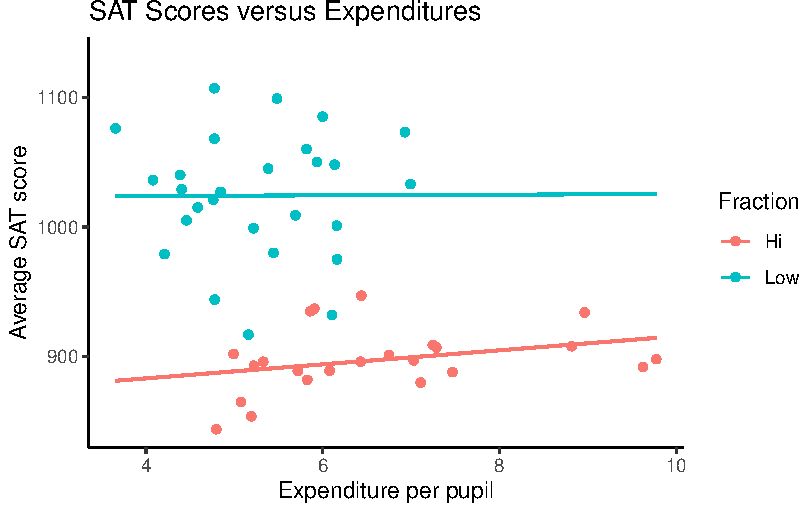
\includegraphics{Studies_files/figure-pdf/fig-conditional-1.pdf}

}

\caption{\label{fig-conditional}Average SAT score versus expenditure per
pupil; broken down by level of participation.}

\end{figure}%

Once we account for the fraction of students taking the SAT, the
relationship between expenditures and SAT scores changes.

In the same way, the \texttt{county} data set is an observational study
with confounding variables, and its data cannot easily be used to make
causal conclusions.

\begin{quote}
\textbf{Exercise}:\\
Figure~\ref{fig-homeown2} shows a negative association between the
homeownership rate and the percentage of multi-unit structures in a
county. However, it is unreasonable to conclude that there is a causal
relationship between the two variables. Suggest one or more other
variables that might explain the relationship in the
Figure~\ref{fig-homeown2}.\footnote{Answers will vary. Population
  density may be important. If a county is very dense, then a larger
  fraction of residents may live in multi-unit structures. Additionally,
  the high density may contribute to increases in property value, making
  homeownership infeasible for many residents.}
\end{quote}

\begin{figure}

\centering{

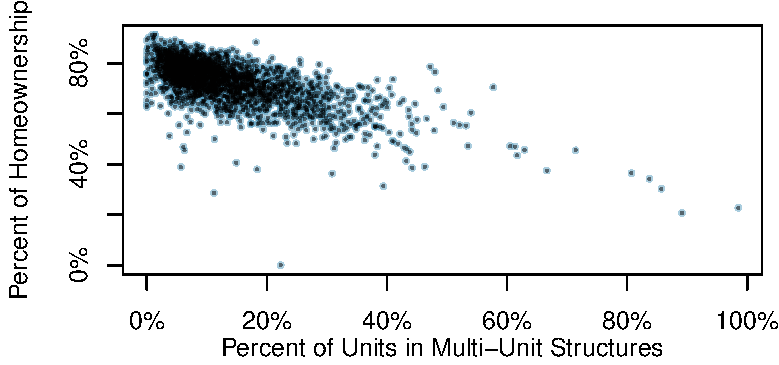
\includegraphics{Studies_files/figure-pdf/fig-homeown2-1.pdf}

}

\caption{\label{fig-homeown2}A scatterplot of the homeownership rate
versus the percent of units that are in multi-unit structures for all
3,143 counties.}

\end{figure}%

Observational studies come in two forms: prospective and retrospective
studies. A \textbf{prospective study} identifies individuals and
collects information as events unfold. For instance, medical researchers
may identify and follow a group of similar individuals over many years
to assess the possible influences of behavior on cancer risk. One
example of such a study is The Nurses Health Study, started in 1976 and
expanded in 1989.\footnote{http://www.channing.harvard.edu/nhs/} This
prospective study recruits registered nurses and then collects data from
them using questionnaires.

\textbf{Retrospective studies} collect data after events have taken
place; e.g.~researchers may review past events in medical records. Some
data sets, such as \texttt{county}, may contain both prospectively- and
retrospectively-collected variables. Local governments prospectively
collect some variables as events unfolded (e.g.~retail sales) while the
federal government retrospectively collected others during the 2010
census (e.g.~county population).

\subsection{Three sampling methods}\label{three-sampling-methods}

Almost all statistical methods are based on the notion of implied
randomness. If observational data are not collected in a random
framework from a population, results from these statistical methods are
not reliable. Here we consider three random sampling techniques: simple,
stratified, and cluster sampling. Figure~\ref{fig-simprand},
Figure~\ref{fig-stratsamp2}, and Figure~\ref{fig-clussamp4} provide a
graphical representation of these techniques.

\begin{figure}

\centering{

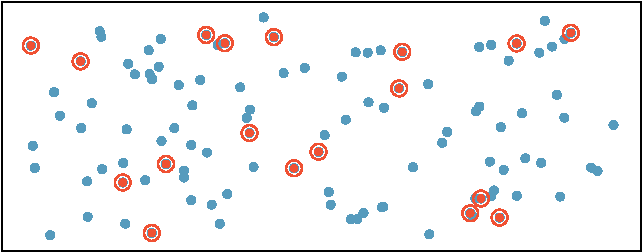
\includegraphics{Studies_files/figure-pdf/fig-simprand-1.pdf}

}

\caption{\label{fig-simprand}Examples of simple random sampling. In this
figure, simple random sampling was used to randomly select the 18
cases.}

\end{figure}%

\begin{figure}

\centering{

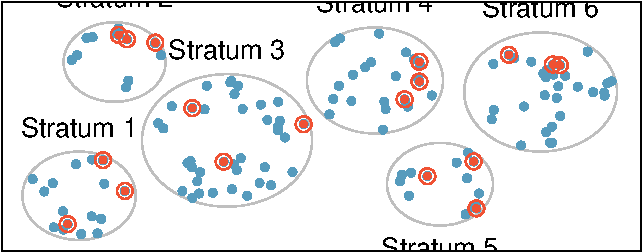
\includegraphics{Studies_files/figure-pdf/fig-stratsamp2-1.pdf}

}

\caption{\label{fig-stratsamp2}In this figure, stratified sampling was
used: cases were grouped into strata, and then simple random sampling
was employed within each stratum.}

\end{figure}%

\begin{figure}

\centering{

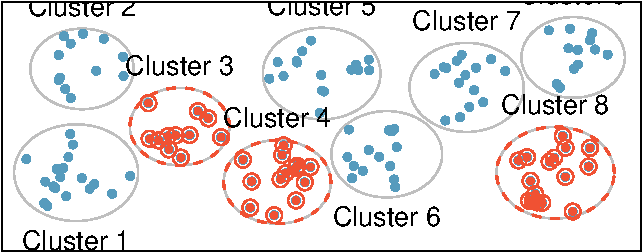
\includegraphics{Studies_files/figure-pdf/fig-clussamp4-1.pdf}

}

\caption{\label{fig-clussamp4}In this figure, cluster sampling was used,
where data were binned into nine clusters, and three of the clusters
were randomly selected.}

\end{figure}%

\textbf{Simple random sampling} is probably the most intuitive form of
random sampling, in which each individual in the population has an equal
chance of being chosen. Consider the salaries of Major League Baseball
(MLB) players, where each player is a member of one of the league's 30
teams. To take a simple random sample of 120 baseball players and their
salaries from the 2010 season, we could write the names of that season's
828 players onto slips of paper, drop the slips into a bucket, shake the
bucket around until we are sure the names are all mixed up, then draw
out slips until we have the sample of 120 players. In general, a sample
is referred to as ``simple random'' if each case in the population has
an equal chance of being included in the final sample \emph{and} knowing
that a case is included in a sample does not provide useful information
about which other cases are included or not.

\textbf{Stratified sampling} is a divide-and-conquer sampling strategy.
The population is divided into groups called \textbf{strata}. The strata
are chosen so that similar cases are grouped together, then a second
sampling method, usually simple random sampling, is employed within each
stratum. In the baseball salary example, the teams could represent the
strata; some teams have a lot more money (we're looking at you,
Yankees). Then we might randomly sample 4 players from each team for a
total of 120 players.

Stratified sampling is especially useful when the cases in each stratum
are very similar with respect to the outcome of interest. The downside
is that analyzing data from a stratified sample is a more complex task
than analyzing data from a simple random sample. The analysis methods
introduced in this book would need to be extended to analyze data
collected using stratified sampling.

\begin{quote}
\textbf{Example}:\\
Why would it be good for cases within each stratum to be very
similar?\footnote{We might get a more stable estimate for the
  subpopulation in a stratum if the cases are very similar. These
  improved estimates for each subpopulation will help us build a
  reliable estimate for the full population.}
\end{quote}

In \textbf{cluster sampling}, we group observations into clusters, then
randomly sample some of the clusters. Sometimes cluster sampling can be
a more economical technique than the alternatives. Also, unlike
stratified sampling, cluster sampling is most helpful when there is a
lot of case-to-case variability within a cluster but the clusters
themselves don't look very different from one another. For example, if
neighborhoods represented clusters, then this sampling method works best
when the neighborhoods are very diverse. A downside of cluster sampling
is that more advanced analysis techniques are typically required, though
the methods in this book can be extended to handle such data.

\begin{quote}
\textbf{Example}:\\
Suppose we are interested in estimating the malaria rate in a densely
tropical portion of rural Indonesia. We learn that there are 30 villages
in that part of the Indonesian jungle, each more or less similar to the
next. What sampling method should be employed?\footnote{A simple random
  sample would likely draw individuals from all 30 villages, which could
  make data collection extremely expensive. Stratified sampling would be
  a challenge since it is unclear how we would build strata of similar
  individuals. However, cluster sampling seems like a very good idea. We
  might randomly select a small number of villages. This would probably
  reduce our data collection costs substantially in comparison to a
  simple random sample and would still give us helpful information.}
\end{quote}

Another technique called \textbf{multistage sampling} is similar to
cluster sampling, except that we take a simple random sample within each
selected cluster. For instance, if we sampled neighborhoods using
cluster sampling, we would next sample a subset of homes within each
selected neighborhood if we were using multistage sampling.

\subsection{Experiments}\label{experiments}

Studies where the researchers assign treatments to cases are called
\textbf{experiments}. When this assignment includes randomization,
e.g.~using a coin flip to decide which treatment a patient receives, it
is called a \textbf{randomized experiment}. Randomized experiments are
fundamentally important when trying to show a causal connection between
two variables.

\subsubsection{Principles of experimental
design}\label{principles-of-experimental-design}

Randomized experiments are generally built on four principles.

\begin{enumerate}
\def\labelenumi{\arabic{enumi}.}
\item
  \textbf{Controlling}. Researchers assign treatments to cases, and they
  do their best to \textbf{control} any other differences in the groups.
  For example, when patients take a drug in pill form, some patients
  take the pill with only a sip of water while others may have it with
  an entire glass of water. To control for the effect of water
  consumption, a doctor may ask all patients to drink a 12 ounce glass
  of water with the pill.
\item
  \textbf{Randomization}. Researchers randomize patients into treatment
  groups to account for variables that cannot be controlled. For
  example, some patients may be more susceptible to a disease than
  others due to their dietary habits. Randomizing patients into the
  treatment or control group helps even out such differences, and it
  also prevents accidental bias from entering the study.
\item
  \textbf{Replication}. The more cases researchers observe, the more
  accurately they can estimate the effect of the explanatory variable on
  the response. In a single study, we \textbf{replicate} by collecting a
  sufficiently large sample. Additionally, a group of scientists may
  replicate an entire study to verify an earlier finding. You replicate
  to the level of variability you want to estimate. For example, in
  flight test, we can run the same flight conditions again to get a
  replicate; however, if the same plane and pilot are being used, the
  replicate is not getting the pilot-to-pilot or the plane-to-plane
  variability.
\item
  \textbf{Blocking}. Researchers sometimes know or suspect that
  variables, other than the treatment, influence the response. Under
  these circumstances, they may first group individuals based on this
  variable and then randomize cases within each block, or group, to the
  treatments. This strategy is often referred to as \textbf{blocking}.
  For instance, if we are looking at the effect of a drug on heart
  attacks, we might first split patients into low-risk and high-risk
  blocks, then randomly assign half the patients from each block to the
  control group and the other half to the treatment group, as shown in
  Figure~\ref{fig-exp4}. This strategy ensures each treatment group has
  an equal number of low-risk and high-risk patients.
\end{enumerate}

\begin{figure}

\centering{

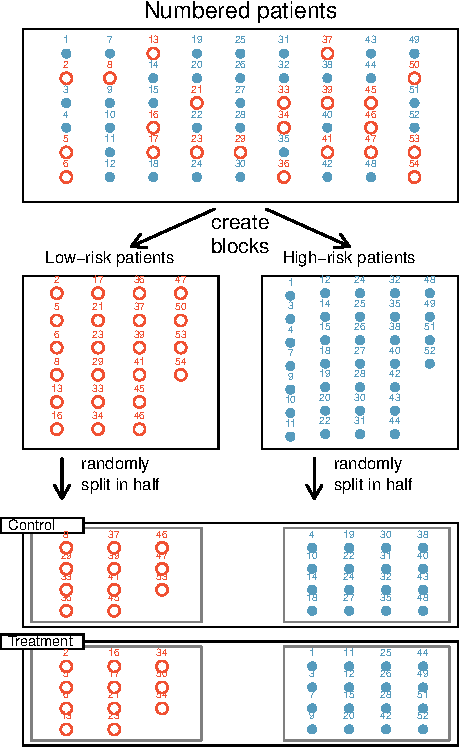
\includegraphics{Studies_files/figure-pdf/fig-exp4-1.pdf}

}

\caption{\label{fig-exp4}Blocking using a variable depicting patient
risk. Patients are first divided into low-risk and high-risk blocks,
then each block is evenly divided into the treatment groups using
randomization. This strategy ensures an equal representation of patients
in each treatment group from both the low-risk and high-risk
categories.}

\end{figure}%

It is important to incorporate the first three experimental design
principles into any study, and this chapter describes methods for
analyzing data from such experiments. Blocking is a slightly more
advanced technique, and statistical methods in this chapter may be
extended to analyze data collected using blocking. Math 359 is an entire
course at USAFA devoted to the design and analysis of experiments.

\subsubsection{Reducing bias in human
experiments}\label{reducing-bias-in-human-experiments}

Randomized experiments are the gold standard for data collection, but
they do not ensure an unbiased perspective into the cause and effect
relationships in all cases. Human studies are perfect examples where
bias can unintentionally arise. Here we reconsider a study where a new
drug was used to treat heart attack patients.\footnote{Anturane
  Reinfarction Trial Research Group. 1980. Sulfinpyrazone in the
  prevention of sudden death after myocardial infarction. New England
  Journal of Medicine 302(5):250-256.} In particular, researchers wanted
to know if the drug reduced deaths in patients.

These researchers designed a randomized experiment because they wanted
to draw causal conclusions about the drug's effect. Study
volunteers\footnote{Human subjects are often called \textbf{patients},
  \textbf{volunteers}, or \textbf{study participants}.} were randomly
placed into two study groups. One group, the \textbf{treatment group},
received the experimental treatment of interest (the new drug to treat
heart attack patients). The other group, called the \textbf{control
group}, did not receive any drug treatment. The comparison between the
treatment and control groups allows researchers to determine whether the
treatment really has an effect.

Put yourself in the place of a person in the study. If you are in the
treatment group, you are given a fancy new drug that you anticipate will
help you. On the other hand, a person in the other group doesn't receive
the drug and sits idly, hoping her participation doesn't increase her
risk of death. These perspectives suggest there are actually two
effects: the one of interest is the effectiveness of the drug, and the
second is an emotional effect that is difficult to quantify.

Researchers aren't usually interested in the emotional effect, which
might bias the study. To circumvent this problem, researchers do not
want patients to know which group they are in. When researchers keep the
patients uninformed about their treatment, the study is said to be
\textbf{blind}. But there is one problem: if a patient doesn't receive a
treatment, she will know she is in the control group. The solution to
this problem is to give fake treatments to patients in the control
group. A fake treatment is called a \textbf{placebo}, and an effective
placebo is the key to making a study truly blind. A classic example of a
placebo is a sugar pill that is made to look like the actual treatment
pill. Often times, a placebo results in a slight but real improvement in
patients. This effect has been dubbed the \textbf{placebo effect}.

The patients are not the only ones who should be blinded: doctors and
researchers can accidentally bias a study. When a doctor knows a patient
has been given the real treatment, she might inadvertently give that
patient more attention or care than a patient that she knows is on the
placebo. To guard against this bias, which again has been found to have
a measurable effect in some instances, most modern studies employ a
\textbf{double-blind} setup where doctors or researchers who interact
with patients are, just like the patients, unaware of who is or is not
receiving the treatment.\footnote{There are always some researchers in
  the study who do know which patients are receiving which treatment.
  However, they do not interact with the study's patients and do not
  tell the blinded health care professionals who is receiving which
  treatment.}

\begin{quote}
\textbf{Exercise}:\\
Look back to the stent study in the first chapter where researchers were
testing whether stents were effective at reducing strokes in at-risk
patients. Is this an experiment? Was the study blinded? Was it
double-blinded?\footnote{The researchers assigned the patients into
  their treatment groups, so this study was an experiment. However, the
  patients could distinguish what treatment they received, so this study
  was not blind. The study could not be double-blind since it was not
  blind.}
\end{quote}

\chapter{Numerical Data}\label{sec-NUMDATA}

\section{Objectives}\label{objectives-5}

\begin{enumerate}
\def\labelenumi{\arabic{enumi})}
\item
  Differentiate between various statistical terminologies such as
  \emph{scatterplot, mean, distribution, point estimate, weighted mean,
  histogram, data density, right skewed, left skewed, symmetric, mode,
  unimodal, bimodal, multimodal, density plot, variance, standard
  deviation, box plot, median, interquartile range, first quartile,
  third quartile, whiskers, outlier, robust estimate}, and
  \emph{transformation}, and construct examples to demonstrate their
  proper use in context.
\item
  Using \texttt{R}, generate and interpret summary statistics for
  numerical variables.
\item
  Create and evaluate graphical summaries of numerical variables using
  \texttt{R}, choosing the most appropriate types of plots for different
  data characteristics and research questions.
\item
  Synthesize numerical and graphical summaries to provide
  interpretations and explanations of a data set.
\end{enumerate}

\section{Numerical Data}\label{numerical-data-1}

This chapter introduces techniques for exploring and summarizing
numerical variables. The \texttt{email50} and \texttt{mlb} data sets
from the \textbf{openintro} package and a subset of
\texttt{county\_complete} from the \textbf{usdata} package provide rich
opportunities for examples. Recall that outcomes of numerical variables
are numbers on which it is reasonable to perform basic arithmetic
operations. For example, the \texttt{pop2010} variable, which represents
the population of counties in 2010, is numerical since we can sensibly
discuss the difference or ratio of the populations in two counties. On
the other hand, area codes and zip codes are not numerical.

\subsection{Scatterplots for paired
data}\label{scatterplots-for-paired-data}

A \textbf{scatterplot} provides a case-by-case view of data for two
numerical variables. In Figure~\ref{fig-scat5}, we again present a
scatterplot used to examine how federal spending and poverty are related
in the \texttt{county} data set.

\begin{figure}

\centering{

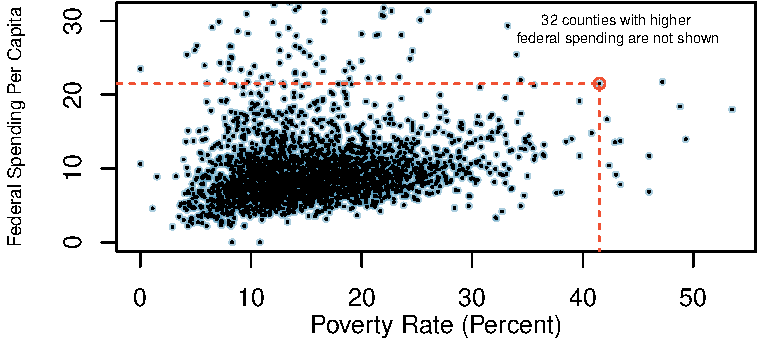
\includegraphics{Numerical-Data_files/figure-pdf/fig-scat5-1.pdf}

}

\caption{\label{fig-scat5}A scatterplot showing fed\_spend against
poverty. Owsley County of Kentucky, with a poverty rate of 41.5\% and
federal spending of \$21.50 per capita, is highlighted.}

\end{figure}%

Another scatterplot is shown in Figure~\ref{fig-scat52}, comparing the
number of \texttt{line\_breaks} and number of characters,
\texttt{num\_char}, in emails for the \texttt{email50} data set. In any
scatterplot, each point represents a single case. Since there are 50
cases in \texttt{email50}, there are 50 points in
Figure~\ref{fig-scat52}.

\begin{figure}

\centering{

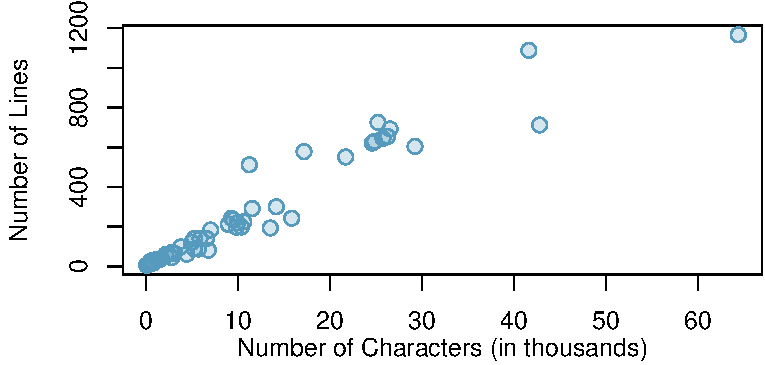
\includegraphics{Numerical-Data_files/figure-pdf/fig-scat52-1.pdf}

}

\caption{\label{fig-scat52}A scatterplot of \texttt{line\_breaks} versus
\texttt{num\_char} for the \texttt{email50} data.}

\end{figure}%

To put the number of characters in perspective, this paragraph in the
text has 357 characters. Looking at Figure~\ref{fig-scat52}, it seems
that some emails are incredibly long! Upon further investigation, we
would actually find that most of the long emails use the HTML format,
which means most of the characters in those emails are used to format
the email rather than provide text.

\begin{quote}
\textbf{Exercise}:\\
What do scatterplots reveal about the data, and how might they be
useful?\footnote{Answers may vary. Scatterplots are helpful in quickly
  spotting associations between variables, whether those associations
  represent simple or more complex relationships.}
\end{quote}

\begin{quote}
\emph{Example}:\\
Consider a new data set of 54 cars with two variables: vehicle price and
weight.\footnote{Subset of data from
  http://www.amstat.org/publications/jse/v1n1/datasets.lock.html} A
scatterplot of vehicle price versus weight is shown in
Figure~\ref{fig-scat53}. What can be said about the relationship between
these variables?
\end{quote}

\begin{figure}

\centering{

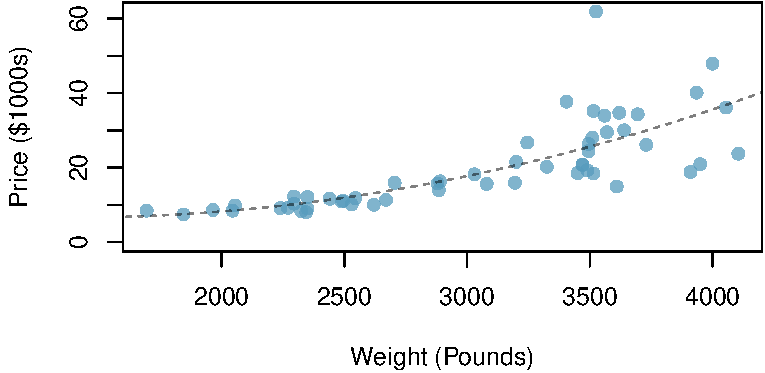
\includegraphics{Numerical-Data_files/figure-pdf/fig-scat53-1.pdf}

}

\caption{\label{fig-scat53}A scatterplot of \emph{price} versus
\emph{weight} for 54 cars.}

\end{figure}%

The relationship is evidently nonlinear, as highlighted by the dashed
line. This is different from previous scatterplots we've seen which show
relationships that are very linear.

\begin{quote}
\textbf{Exercise}:\\
Describe two variables that would have a horseshoe-shaped association in
a scatterplot.\footnote{Consider the case where your vertical axis
  represents something ``good'' and your horizontal axis represents
  something that is only good in moderation. Health and water
  consumption fit this description since water becomes toxic when
  consumed in excessive quantities.}
\end{quote}

\subsection{The mean}\label{the-mean}

The \textbf{mean}, sometimes called the average, is a common way to
measure the center of a \textbf{distribution}\footnote{The distribution
  of a variable is essentially the collection of all values of the
  variable in the data set. It tells us what values the variable takes
  on and how often. In the \texttt{email50} data set, we used a dotplot
  to view the distribution of \texttt{num\_char}.} of data. To find the
mean number of characters in the 50 emails, we add up all the character
counts and divide by the number of emails. For computational
convenience, the number of characters is listed in the thousands and
rounded to the first decimal.

\[\bar{x} = \frac{21.7 + 7.0 + \cdots + 15.8}{50} = 11.6\]

The sample mean is often labeled \(\bar{x}\). There is a bar over the
letter, and the letter \(x\) is being used as a generic placeholder for
the variable of interest, \texttt{num\_char}.

\begin{quote}
\textbf{Mean}\\
The sample mean of a numerical variable is the sum of all of the
observations divided by the number of observations, Equation 1.
\end{quote}

\begin{equation} 
  \bar{x} = \frac{x_1+x_2+\cdots+x_n}{n}
  \tag{1}
\end{equation}

where \(x_1, x_2, \dots, x_n\) represent the \(n\) observed values.

\begin{quote}
\textbf{Exercise}:\\
Examine the two equations above. What does \(x_1\) correspond to? And
\(x_2\)? Can you infer a general meaning to what \(x_i\) might
represent?\footnote{\(x_1\) corresponds to the number of characters in
  the first email in the sample (21.7, in thousands), \(x_2\) to the
  number of characters in the second email (7.0, in thousands), and
  \(x_i\) corresponds to the number of characters in the \(i^{th}\)
  email in the data set.}
\end{quote}

\begin{quote}
\textbf{Exercise}:\\
What was \(n\) in this sample of emails?\footnote{The sample size,
  \(n = 50\).}
\end{quote}

The \texttt{email50} data set is a sample from a larger population of
emails that were received in January and March. We could compute a mean
for this population in the same way as the sample mean. However, there
is a difference in notation: the population mean has a special label:
\(\mu\). The symbol \(\mu\) is the Greek letter \emph{mu} and represents
the average of all observations in the population. Sometimes a
subscript, such as \(_x\), is used to represent which variable the
population mean refers to, e.g.~\(\mu_x\).

\begin{quote}
\emph{Example}: The average number of characters across all emails can
be estimated using the sample data. Based on the sample of 50 emails,
what would be a reasonable estimate of \(\mu_x\), the mean number of
characters in all emails in the \texttt{email} data set? (Recall that
\texttt{email50} is a sample from \texttt{email}.)
\end{quote}

The sample mean, 11.6, may provide a reasonable estimate of \(\mu_x\).
While this number will not be perfect, it provides a \textbf{point
estimate}, a single plausible value, of the population mean. Later in
the text, we will develop tools to characterize the accuracy of point
estimates, and we will find that point estimates based on larger samples
tend to be more accurate than those based on smaller samples.

\begin{quote}
\emph{Example}:\\
We might like to compute the average income per person in the US. To do
so, we might first think to take the mean of the per capita incomes from
the 3,143 counties in the \texttt{county} data set. What would be a
better approach?
\end{quote}

The \texttt{county} data set is special in that each county actually
represents many individual people. If we were to simply average across
the \texttt{income} variable, we would be treating counties with 5,000
and 5,000,000 residents equally in the calculations. Instead, we should
compute the total income for each county, add up all the counties'
totals, and then divide by the number of people in all the counties. If
we completed these steps with the \texttt{county} data, we would find
that the per capita income for the US is \$27,348.43. Had we computed
the \emph{simple} mean of per capita income across counties, the result
would have been just \$22,504.70!

This previous example used what is called a \textbf{weighted
mean}\footnote{A weighted mean is an average in which some observations
  contribute more ``weight'' than others. In the \texttt{county} data
  set, we ``weighted'' the income for each county by dividing income by
  the county population.}, which will be a key topic in the probability
section. As a look ahead, the probability mass function gives the
population proportions of each county's mean value, and thus, to find
the population mean \(\mu\), we will use a weighted mean.

\subsection{Histograms and shape}\label{histograms-and-shape}

Rather than showing the exact value of each observation for a single
variable, think of the value as belonging to a \emph{bin}. For example,
in the \texttt{email50} data set, we create a table of counts for the
number of cases with character counts between 0 and 5,000, then the
number of cases between 5,000 and 10,000, and so on. Observations that
fall on the boundary of a bin (e.g.~5,000) are allocated to the lower
bin. This tabulation is shown below.

\begin{verbatim}

  (0,5]  (5,10] (10,15] (15,20] (20,25] (25,30] (30,35] (35,40] (40,45] (45,50] 
     19      12       6       2       3       5       0       0       2       0 
(50,55] (55,60] (60,65] 
      0       0       1 
\end{verbatim}

These binned counts are plotted as bars in Figure~\ref{fig-hist5} in
what is called a \textbf{histogram}\footnote{A histogram displays the
  distribution of a quantitative variable. It shows binned counts, the
  number of observations in a bin, or range of values.}.

\begin{figure}

\centering{

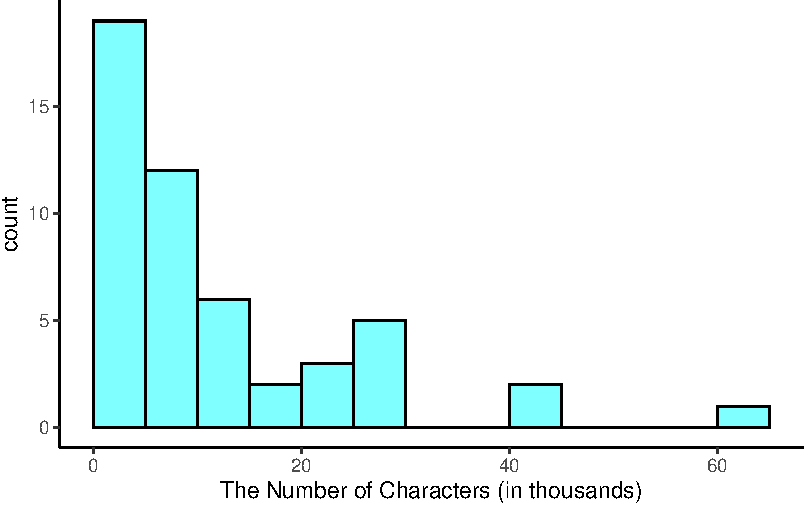
\includegraphics{Numerical-Data_files/figure-pdf/fig-hist5-1.pdf}

}

\caption{\label{fig-hist5}A histogram of \texttt{num\_char}. This
distribution is very strongly skewed to the right.}

\end{figure}%

Histograms provide a view of the \textbf{data density}. Higher bars
represent where the data are relatively more dense. For instance, there
are many more emails between 0 and 10,000 characters than emails between
10,000 and 20,000 characters in the data set. The bars make it easy to
see how the density of the data changes relative to the number of
characters.

Histograms are especially convenient for describing the shape of the
data distribution. Figure~\ref{fig-hist5} shows that most emails have a
relatively small number of characters, while fewer emails have a very
large number of characters. When data trail off to the right in this way
and have a longer right \textbf{tail}, the shape is said to be
\textbf{right skewed}.\footnote{Other ways to describe data that are
  skewed to the right: \textbf{skewed to the right}, \textbf{skewed to
  the high end}, or \textbf{skewed to the positive end}.}

Data sets with the reverse characteristic -- a long, thin tail to the
left -- are said to be \textbf{left skewed}. We also say that such a
distribution has a long left tail. Data sets that show roughly equal
trailing off in both directions are called \textbf{symmetric}.

\begin{quote}
\textbf{Long tails to identify skew}\\
When data trail off in one direction, the distribution has a
\textbf{long tail}. If a distribution has a long left tail, it is left
skewed. If a distribution has a long right tail, it is right skewed.
\end{quote}

\subsubsection{Making our own histogram}\label{making-our-own-histogram}

Let's take some time to make a simple histogram. We will use the
\textbf{ggformula} package, which is a wrapper for the \textbf{ggplot2}
package.

Here are two questions:\\
\emph{What do we want \texttt{R} to do?} and\\
\emph{What must we give \texttt{R} for it to do this?}

We want \texttt{R} to make a histogram. In \texttt{ggformula}, the plots
have the form \texttt{gf\_plottype} so we will use the
\texttt{gf\_histogram()}. To find options and more information about the
function, type:

\begin{verbatim}
?gf_histogram
\end{verbatim}

To start, we just have to give the formulas and data to \texttt{R}.

\begin{Shaded}
\begin{Highlighting}[]
\FunctionTok{gf\_histogram}\NormalTok{(}\SpecialCharTok{\textasciitilde{}}\NormalTok{num\_char, }\AttributeTok{data =}\NormalTok{ email50, }\AttributeTok{color =} \StringTok{"black"}\NormalTok{, }\AttributeTok{fill =} \StringTok{"cyan"}\NormalTok{)}
\end{Highlighting}
\end{Shaded}

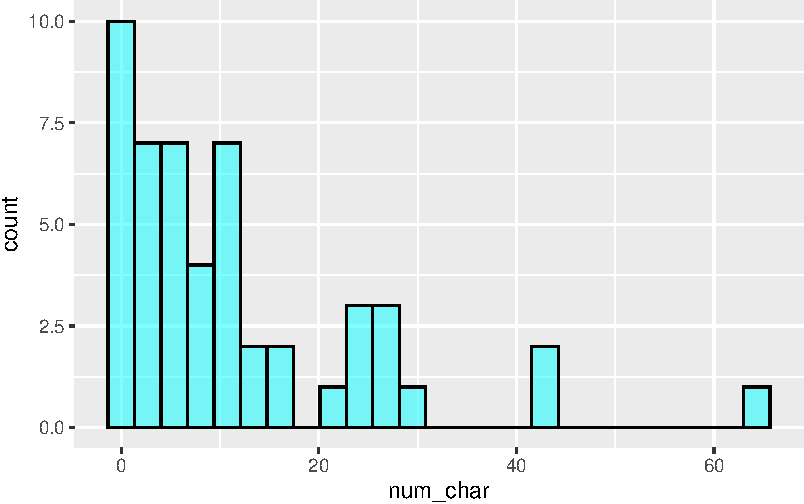
\includegraphics{Numerical-Data_files/figure-pdf/unnamed-chunk-8-1.pdf}

\begin{quote}
\textbf{Exercise}:\\
Look at the help menu for \texttt{gf\_histogram} and change the x-axis
label, change the bin width to 5, and have the left bin start at 0.
\end{quote}

Here is the code for the exercise:

\begin{verbatim}
email50 %>%
   gf_histogram(~num_char, binwidth = 5,boundary = 0,
   xlab = "The Number of Characters (in thousands)", 
   color = "black", fill = "cyan") %>%
   gf_theme(theme_classic())
\end{verbatim}

In addition to looking at whether a distribution is skewed or symmetric,
histograms can be used to identify modes. A \textbf{mode} is represented
by a prominent peak in the distribution.\footnote{Another definition of
  mode, which is not typically used in statistics, is the value with the
  most occurrences. It is common to have \emph{no} observations with the
  same value in a data set, which makes this other definition useless
  for many real data sets.} There is only one prominent peak in the
histogram of \texttt{num\_char}.

Figure~\ref{fig-histmulti} shows histograms that have one, two, or three
prominent peaks. Such distributions are called \textbf{unimodal},
\textbf{bimodal}, and \textbf{multimodal}, respectively. Any
distribution with more than 2 prominent peaks is called multimodal.
Notice that there was one prominent peak in the unimodal distribution
with a second less prominent peak that was not counted since the
separation between the two peaks is relatively small, and it only
differs from its neighboring bins by a few observations.

\begin{figure}

\centering{

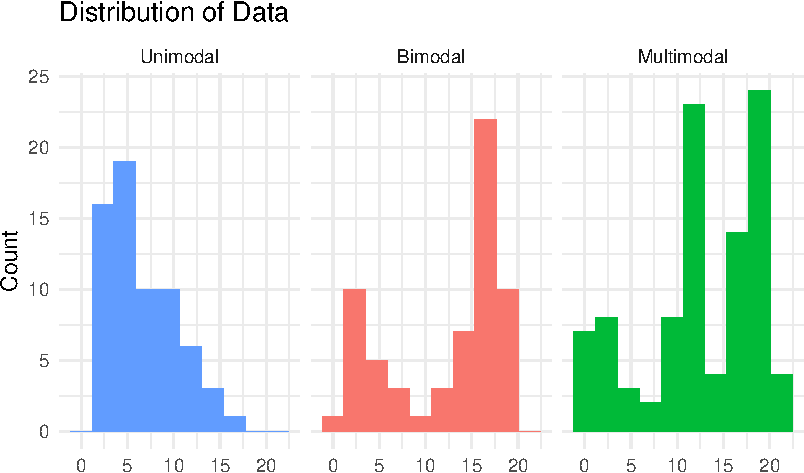
\includegraphics{Numerical-Data_files/figure-pdf/fig-histmulti-1.pdf}

}

\caption{\label{fig-histmulti}Histograms that demonstrate unimodal,
bimodal, and multimodal data.}

\end{figure}%

\begin{quote}
\textbf{Exercise}:\\
Height measurements of young students and adult teachers at a K-3
elementary school were taken. How many modes would you anticipate in
this height data set?\footnote{There might be two height groups visible
  in the data set: one for the students and one for the adults. That is,
  the data are probably bimodal. But it could be multimodal because
  within each group we may be able to see a difference in males and
  females.}
\end{quote}

\begin{quote}
\textbf{Looking for modes}\\
Looking for modes isn't about finding a clear and correct answer about
the number of modes in a distribution, which is why \textbf{prominent}
is not rigorously defined in these notes. The important part of this
examination is to better understand your data and how it might be
structured.
\end{quote}

\subsection{Density plots}\label{density-plots}

Another useful plotting method uses \textbf{density plots} to visualize
numerical data. A histogram bins data but is highly dependent on the
number and boundary of the bins. A density plot also estimates the
distribution of a numerical variable but does this by estimating the
density of data points in a small window around each data point. The
overall curve is the sum of this small density estimate. A density plot
can be thought of as a smooth version of the histogram. Several options
go into a density estimate, such as the width of the window and type of
smoothing function. These ideas are beyond the scope here and we will
just use the default options. Figure~\ref{fig-dens5} shows the same
distribution of the number of characters but in a smoother way than a
histogram.

\begin{figure}

\centering{

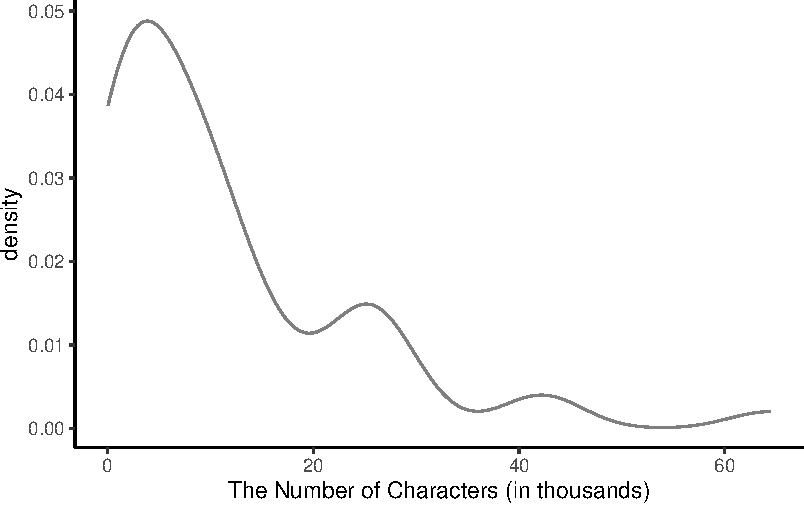
\includegraphics{Numerical-Data_files/figure-pdf/fig-dens5-1.pdf}

}

\caption{\label{fig-dens5}A histogram of \texttt{num\_char}. This
distribution is very strongly skewed to the right.}

\end{figure}%

\begin{quote}
\textbf{Exercise}:\\
Compare and contrast the histogram in Figure~\ref{fig-hist5} and the
density plot in Figure~\ref{fig-dens5}. What can you see in the
histogram you can't see in the density plot?
\end{quote}

\subsection{Variance and standard
deviation}\label{variance-and-standard-deviation}

The mean is used to describe the center of a data set, but the
\emph{variability} in the data is also important. Here, we introduce two
measures of variability: the \textbf{variance} and the \textbf{standard
deviation}. Both of these are very useful in data analysis, even though
the formulas are a bit tedious to calculate by hand. The standard
deviation is the easier of the two to conceptually understand; it
roughly describes how far away the typical observation is from the mean.
Equation 2 is the equation for sample variance. We will demonstrate it
with data so that the notation is easier to understand.

\begin{align}
s_{}^2 &= \sum_{i = 1}^{n} \frac{(x_i - \bar{x})^2}{n - 1} \\
    &= \frac{(x_1 - \bar{x})^2 + (x_2 - \bar{x})^2 + (x_3 - \bar{x})^2 + \cdots + (x_n - \bar{x})^2}{n - 1} 
  \tag{2}
\end{align}

where \(x_1, x_2, \dots, x_n\) represent the \(n\) observed values.

We call the distance of an observation from its mean the
\textbf{deviation}. Below are the deviations for the \(1^{st}\),
\(2^{nd}\), \(3^{rd}\), and \(50^{th}\) observations of the
\texttt{num\_char} variable. For computational convenience, the number
of characters is listed in the thousands and rounded to the first
decimal.

\[
\begin{aligned}
x_1^{}-\bar{x} &= 21.7 - 11.6 = 10.1 \hspace{5mm}\text{ } \\
x_2^{}-\bar{x} &= 7.0 - 11.6 = -4.6 \\
x_3^{}-\bar{x} &= 0.6 - 11.6 = -11.0 \\
            &\ \vdots \\
x_{50}^{}-\bar{x} &= 15.8 - 11.6 = 4.2
\end{aligned}
\]

If we square these deviations and then take an average, the result is
equal to the \textbf{sample variance}, denoted by \(s_{}^2\):

\[
\begin{aligned}
s_{}^2 &= \frac{10.1_{}^2 + (-4.6)_{}^2 + (-11.0)_{}^2 + \cdots + 4.2_{}^2}{50-1} \\
    &= \frac{102.01 + 21.16 + 121.00 + \cdots + 17.64}{49} \\
    &= 172.44
\end{aligned}
\]

We divide by \(n - 1\), rather than dividing by \(n\), when computing
the variance; you need not worry about this mathematical nuance yet.
Notice that squaring the deviations does two things. First, it makes
large values much larger, seen by comparing \(10.1^2\), \((-4.6)^2\),
\((-11.0)^2\), and \(4.2^2\). Second, it gets rid of any negative signs.

The sample \textbf{standard deviation}, \(s\), is the square root of the
variance:

\[s = \sqrt{172.44} = 13.13\]

The sample standard deviation of the number of characters in an email is
13.13 thousand. A subscript of \(_x\) may be added to the variance and
standard deviation, i.e.~\(s_x^2\) and \(s_x^{}\), as a reminder that
these are the variance and standard deviation of the observations
represented by \(x_1^{}\), \(x_2^{}\), \ldots, \(x_n^{}\). The \(_{x}\)
subscript is usually omitted when it is clear which data the variance or
standard deviation is referencing.

\begin{quote}
\textbf{Variance and standard deviation}\\
The variance is roughly the average squared distance from the mean. The
standard deviation is the square root of the variance and describes how
close the data are to the mean.
\end{quote}

Formulas and methods used to compute the variance and standard deviation
for a population are similar to those used for a sample.\footnote{The
  only difference is that the population variance has a division by
  \(n\) instead of \(n - 1\).} However, like the mean, the population
values have special symbols: \(\sigma_{}^2\) for the variance and
\(\sigma\) for the standard deviation. The symbol \(\sigma\) is the
Greek letter \emph{sigma}.

\begin{quote}
\textbf{Tip: standard deviation describes variability}\\
Focus on the conceptual meaning of the standard deviation as a
descriptor of variability rather than the formulas. Usually 70\% of the
data will be within one standard deviation of the mean and about 95\%
will be within two standard deviations. However, as we have seen, these
percentages are not strict rules.
\end{quote}

\begin{figure}

\centering{

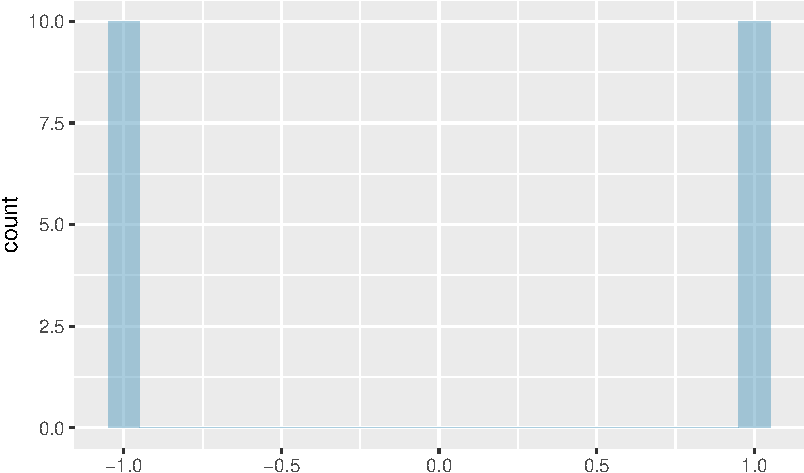
\includegraphics{Numerical-Data_files/figure-pdf/fig-hist53-1.pdf}

}

\caption{\label{fig-hist53}The first of three very different population
distributions with the same mean, 0, and standard deviation, 1.}

\end{figure}%

\begin{figure}

\centering{

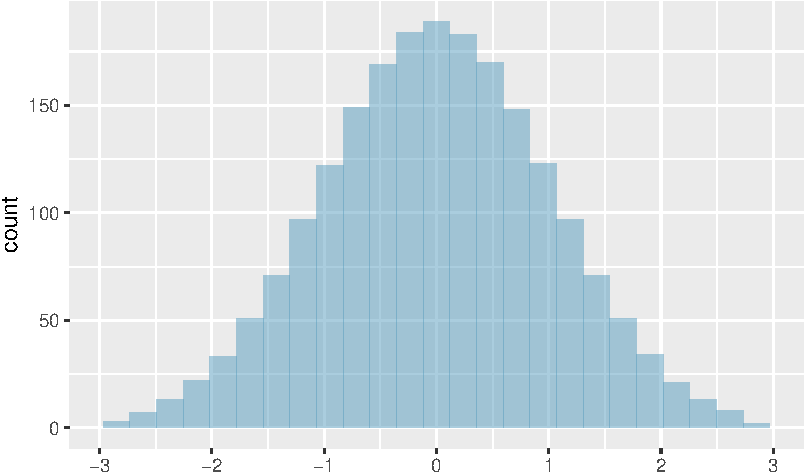
\includegraphics{Numerical-Data_files/figure-pdf/fig-hist54-1.pdf}

}

\caption{\label{fig-hist54}The second plot with mean 0 and standard
deviation 1.}

\end{figure}%

\begin{figure}

\centering{

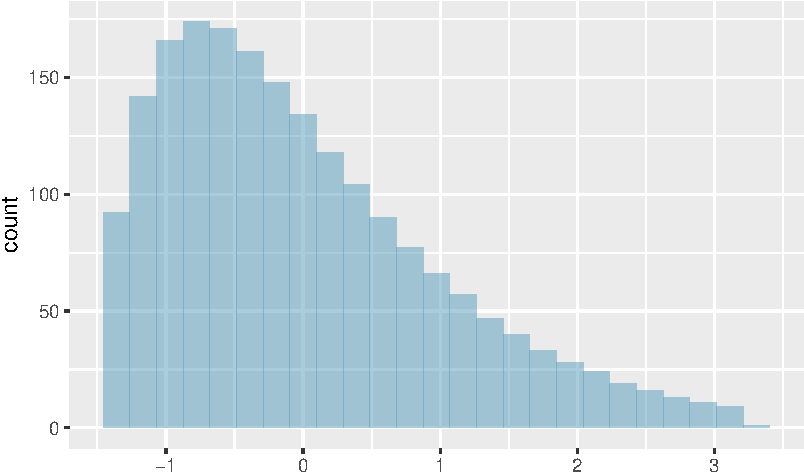
\includegraphics{Numerical-Data_files/figure-pdf/fig-hist55-1.pdf}

}

\caption{\label{fig-hist55}The final plot with mean 0 and standard
deviation 1.}

\end{figure}%

\begin{quote}
\textbf{Exercise}:\\
Earlier, the concept of shape of a distribution was introduced. A good
description of the shape of a distribution should include modality and
whether the distribution is symmetric or skewed to one side. Using the
three figures,
Figures~\ref{fig-hist53}, \ref{fig-hist54}, \ref{fig-hist55} as
examples, explain why such a description is important.\footnote{Starting
  with Figure @ref(fig:hist53-fig), the three figures show three
  distributions that look quite different, but all have the same mean,
  variance, and standard deviation. Using modality, we can distinguish
  between the first plot (bimodal) and the last two (unimodal). Using
  skewness, we can distinguish between the last plot (right skewed) and
  the first two. While a picture, like a histogram, tells a more
  complete story, we can use modality and shape (symmetry/skew) to
  characterize basic information about a distribution.}
\end{quote}

\begin{quote}
\emph{Example}:\\
Describe the distribution of the \texttt{num\_char} variable using the
histogram in Figure~\ref{fig-hist5}. The description should incorporate
the center, variability, and shape of the distribution, and it should
also be placed in context: the number of characters in emails. Also note
any especially unusual cases/observations.\footnote{The distribution of
  email character counts is unimodal and very strongly skewed to the
  high end (right skewed). Many of the counts fall near the mean at
  11,600, and most fall within one standard deviation (13,130) of the
  mean. There is one exceptionally long email with about 65,000
  characters.}
\end{quote}

In practice, the variance and standard deviation are sometimes used as a
means to an end, where the \emph{end} is being able to accurately
estimate the uncertainty associated with a sample statistic. For
example, later in the book we will use the variance and standard
deviation to assess how close the sample mean is to the population mean.

\subsection{Box plots, quartiles, and the
median}\label{box-plots-quartiles-and-the-median}

A \textbf{box plot} summarizes a data set using five statistics, while
also plotting unusual observations. Figure~\ref{fig-box} provides an
annotated vertical dot plot alongside a box plot of the
\texttt{num\_char} variable from the \texttt{email50} data set.

\begin{figure}

\centering{

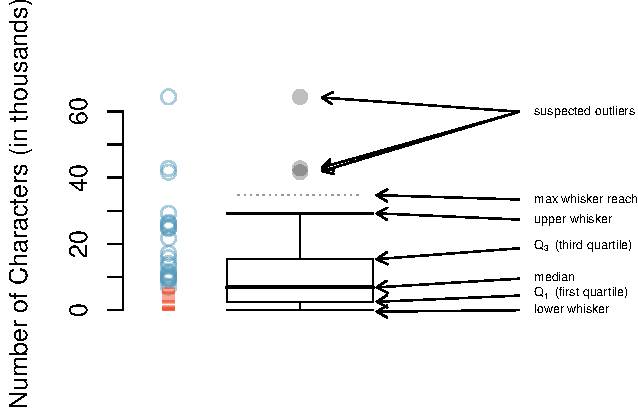
\includegraphics{Numerical-Data_files/figure-pdf/fig-box-1.pdf}

}

\caption{\label{fig-box}A vertical dot plot next to a labeled box plot
for the number of characters in 50 emails. The median (6,890), splits
the data into the bottom 50\% and the top 50\%, marked in the dot plot
by horizontal dashes and open circles, respectively.}

\end{figure}%

The first step in building a box plot is drawing a dark line denoting
the \textbf{median}, which splits the data in half. Figure~\ref{fig-box}
shows 50\% of the data falling below the median (red dashes) and the
other 50\% falling above the median (blue open circles). There are 50
character counts in the data set (an even number) so the data are
perfectly split into two groups of 25. We take the median in this case
to be the average of the two observations closest to the \(50^{th}\)
percentile: \((\text{6,768} + \text{7,012}) / 2 = \text{6,890}\). When
there are an odd number of observations, there will be exactly one
observation that splits the data into two halves, and in this case that
observation is the median (no average needed).

\begin{quote}
\textbf{Median: the number in the middle}\\
If the data are ordered from smallest to largest, the \textbf{median} is
the observation in the middle. If there are an even number of
observations, there will be two values in the middle, and the median is
taken as their average.
\end{quote}

The second step in building a box plot is drawing a rectangle to
represent the middle 50\% of the data. The total length of the box,
shown vertically in Figure~\ref{fig-box}, is called the
\textbf{interquartile range} (IQR, for short). It, like the standard
deviation, is a measure of variability in the data. The more variable
the data, the larger the standard deviation and IQR. The two boundaries
of the box are called the \textbf{first quartile} (the \(25^{th}\)
percentile, i.e.~25\% of the data fall below this value) and the
\textbf{third quartile} (the \(75^{th}\) percentile), and these are
often labeled \(Q_1\) and \(Q_3\), respectively.

\begin{quote}
\textbf{Interquartile range (IQR)}\\
The IQR is the length of the box in a box plot. It is computed as
\[ IQR = Q_3 - Q_1 \] where \(Q_1\) and \(Q_3\) are the \(25^{th}\) and
\(75^{th}\) percentiles, respectively.
\end{quote}

\begin{quote}
\textbf{Exercise}:\\
What percent of the data fall between \(Q_1\) and the median? What
percent is between the median and \(Q_3\)?\footnote{Since \(Q_1\) and
  \(Q_3\) capture the middle 50\% of the data and the median splits the
  data in the middle, 25\% of the data fall between \(Q_1\) and the
  median, and another 25\% fall between the median and \(Q_3\).}
\end{quote}

Extending out from the box, the \textbf{whiskers} attempt to capture the
data outside of the box, however, their reach is never allowed to be
more than \(1.5\times IQR\).\footnote{While the choice of exactly 1.5 is
  arbitrary, it is the most commonly used value for box plots.} They
capture everything within this reach. In Figure~\ref{fig-box}, the upper
whisker does not extend to the last three points, which are beyond
\(Q_3 + 1.5\times IQR\), and so it extends only to the last point below
this limit. The lower whisker stops at the lowest value, 33, since there
is no additional data to reach; the lower whisker's limit is not shown
in the figure because the plot does not extend down to
\(Q_1 - 1.5\times IQR\). In a sense, the box is like the body of the box
plot and the whiskers are like its arms trying to reach the rest of the
data.

Any observation that lies beyond the whiskers is labeled with a dot. The
purpose of labeling these points -- instead of just extending the
whiskers to the minimum and maximum observed values -- is to help
identify any observations that appear to be unusually distant from the
rest of the data. Unusually distant observations are called
\textbf{outliers}. In this case, it would be reasonable to classify the
emails with character counts of 41,623, 42,793, and 64,401 as outliers
since they are numerically distant from most of the data.

\begin{quote}
\textbf{Outliers are extreme}\\
An \textbf{outlier} is an observation that is extreme, relative to the
rest of the data.
\end{quote}

\begin{quote}
\textbf{Why it is important to look for outliers}\\
Examination of data for possible outliers serves many useful purposes,
including:\\
1. Identifying \textbf{strong skew} in the distribution.\\
2. Identifying data collection or entry errors. For instance, we
re-examined the email purported to have 64,401 characters to ensure this
value was accurate.\\
3. Providing insight into interesting properties of the data.
\end{quote}

\begin{quote}
\textbf{Exercise}:\\
The observation with value 64,401, an outlier, was found to be an
accurate observation. What would such an observation suggest about the
nature of character counts in emails?\footnote{That occasionally there
  may be very long emails.}
\end{quote}

\begin{quote}
\textbf{Exercise}:\\
Using Figure~\ref{fig-box}, estimate the following values for
\texttt{num\_char} in the \texttt{email50} data set:\\
(a) \(Q_1\),\\
(b) \(Q_3\), and\\
(c) IQR.\footnote{These visual estimates will vary a little from one
  person to the next: \(Q_1\) \textasciitilde{} 3,000, \(Q_3\)
  \textasciitilde{} 15,000, IQR = \(Q_3 - Q_1\) \textasciitilde{}
  12,000. (The true values: \$Q\_1 = \$ 2,536, \$Q\_3 = \$ 15,411, IQR =
  12,875.)}
\end{quote}

Of course, \texttt{R} can calculate these summary statistics for us.
First, we will do these calculations individually and then in one
function call. Remember to ask yourself what you want \texttt{R} to do
and what it needs to do this.

\begin{Shaded}
\begin{Highlighting}[]
\FunctionTok{mean}\NormalTok{(}\SpecialCharTok{\textasciitilde{}}\NormalTok{num\_char, }\AttributeTok{data =}\NormalTok{ email50)}
\end{Highlighting}
\end{Shaded}

\begin{verbatim}
[1] 11.59822
\end{verbatim}

\begin{Shaded}
\begin{Highlighting}[]
\FunctionTok{sd}\NormalTok{(}\SpecialCharTok{\textasciitilde{}}\NormalTok{num\_char, }\AttributeTok{data =}\NormalTok{ email50)}
\end{Highlighting}
\end{Shaded}

\begin{verbatim}
[1] 13.12526
\end{verbatim}

\begin{Shaded}
\begin{Highlighting}[]
\FunctionTok{quantile}\NormalTok{(}\SpecialCharTok{\textasciitilde{}}\NormalTok{num\_char, }\AttributeTok{data =}\NormalTok{ email50)}
\end{Highlighting}
\end{Shaded}

\begin{verbatim}
      0%      25%      50%      75%     100% 
 0.05700  2.53550  6.88950 15.41075 64.40100 
\end{verbatim}

\begin{Shaded}
\begin{Highlighting}[]
\FunctionTok{iqr}\NormalTok{(}\SpecialCharTok{\textasciitilde{}}\NormalTok{num\_char, }\AttributeTok{data =}\NormalTok{ email50)}
\end{Highlighting}
\end{Shaded}

\begin{verbatim}
[1] 12.87525
\end{verbatim}

\begin{Shaded}
\begin{Highlighting}[]
\FunctionTok{favstats}\NormalTok{(}\SpecialCharTok{\textasciitilde{}}\NormalTok{num\_char, }\AttributeTok{data =}\NormalTok{ email50)}
\end{Highlighting}
\end{Shaded}

\begin{verbatim}
   min     Q1 median       Q3    max     mean       sd  n missing
 0.057 2.5355 6.8895 15.41075 64.401 11.59822 13.12526 50       0
\end{verbatim}

\subsection{Robust statistics}\label{robust-statistics}

How are the \emph{sample statistics} of the \texttt{num\_char} data set
affected by the observation with value 64,401? What would we see if this
email wasn't present in the data set? What would happen to these
\emph{summary statistics} if the observation at 64,401 had been even
larger, say 150,000? These scenarios are plotted alongside the original
data in Figure~\ref{fig-box2}, and sample statistics are computed in
\texttt{R}.

First, we create a new data frame containing the three scenarios: 1) the
original data, 2) the data with the extreme observation dropped, and 3)
the data with the extreme observation increased.

\begin{Shaded}
\begin{Highlighting}[]
\CommentTok{\# code to create the \textasciigrave{}robust\textasciigrave{} data frame}
\NormalTok{p1 }\OtherTok{\textless{}{-}}\NormalTok{ email50}\SpecialCharTok{$}\NormalTok{num\_char}
\NormalTok{p2 }\OtherTok{\textless{}{-}}\NormalTok{ p1[}\SpecialCharTok{{-}}\FunctionTok{which.max}\NormalTok{(p1)]}
\NormalTok{p3 }\OtherTok{\textless{}{-}}\NormalTok{ p1}
\NormalTok{p3[}\FunctionTok{which.max}\NormalTok{(p1)] }\OtherTok{\textless{}{-}} \DecValTok{150}

\NormalTok{robust }\OtherTok{\textless{}{-}} \FunctionTok{data.frame}\NormalTok{(}\AttributeTok{value =} \FunctionTok{c}\NormalTok{(p1, p2, p3),}
                     \AttributeTok{group =} \FunctionTok{c}\NormalTok{(}\FunctionTok{rep}\NormalTok{(}\StringTok{"Original"}\NormalTok{, }\DecValTok{50}\NormalTok{),}
                             \FunctionTok{rep}\NormalTok{(}\StringTok{"Dropped"}\NormalTok{, }\DecValTok{49}\NormalTok{), }\FunctionTok{rep}\NormalTok{(}\StringTok{"Increased"}\NormalTok{, }\DecValTok{50}\NormalTok{)))}
\FunctionTok{head}\NormalTok{(robust)}
\end{Highlighting}
\end{Shaded}

\begin{verbatim}
   value    group
1 21.705 Original
2  7.011 Original
3  0.631 Original
4  2.454 Original
5 41.623 Original
6  0.057 Original
\end{verbatim}

Now, we create a side-by-side boxplots for each scenario.

\begin{Shaded}
\begin{Highlighting}[]
\FunctionTok{gf\_boxplot}\NormalTok{(value }\SpecialCharTok{\textasciitilde{}}\NormalTok{ group, }\AttributeTok{data =}\NormalTok{ robust, }\AttributeTok{xlab =} \StringTok{"Data Group"}\NormalTok{,}
           \AttributeTok{ylab =} \StringTok{"Number of Characters (in thousands)"}\NormalTok{) }\SpecialCharTok{\%\textgreater{}\%}
   \FunctionTok{gf\_theme}\NormalTok{(}\FunctionTok{theme\_classic}\NormalTok{())}
\end{Highlighting}
\end{Shaded}

\begin{figure}[H]

\centering{

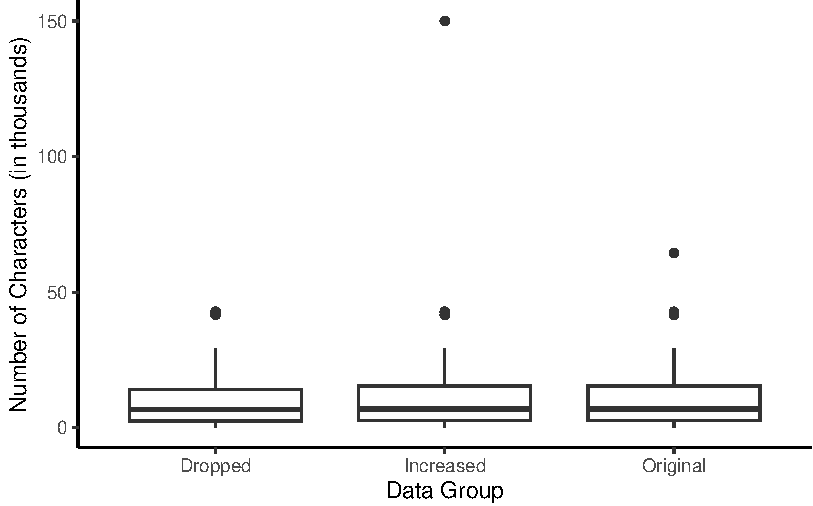
\includegraphics{Numerical-Data_files/figure-pdf/fig-box2-1.pdf}

}

\caption{\label{fig-box2}Box plots of the original character count data
and two modified data sets, one where the outlier at 64,401 is dropped
and one where its value is increased.}

\end{figure}%

We can also use \texttt{favstats()} to calculate summary statistics of
\texttt{value} by \texttt{group}, using the \texttt{robust} data frame
created above.

\begin{Shaded}
\begin{Highlighting}[]
\FunctionTok{favstats}\NormalTok{(value }\SpecialCharTok{\textasciitilde{}}\NormalTok{ group, }\AttributeTok{data =}\NormalTok{ robust)}
\end{Highlighting}
\end{Shaded}

\begin{verbatim}
      group   min     Q1 median       Q3     max     mean       sd  n missing
1   Dropped 0.057 2.4540 6.7680 14.15600  42.793 10.52061 10.79768 49       0
2 Increased 0.057 2.5355 6.8895 15.41075 150.000 13.31020 22.43436 50       0
3  Original 0.057 2.5355 6.8895 15.41075  64.401 11.59822 13.12526 50       0
\end{verbatim}

Notice by using the formula notation, we were able to calculate the
summary statistics within each group.

\begin{quote}
\textbf{Exercise}:\\
(a) Which is affected more by extreme observations, the mean or median?
The data summary may be helpful.\footnote{The mean is affected more.}\\
(b) Which is affected more by extreme observations, the standard
deviation or IQR?\footnote{The standard deviation is affected more.}
\end{quote}

The median and IQR are called \textbf{robust statistics} because extreme
observations have little effect on their values. The mean and standard
deviation are affected much more by changes in extreme observations.

\begin{quote}
\emph{Example}:\\
The median and IQR do not change much under the three scenarios above.
Why might this be the case?\footnote{The median and IQR are only
  sensitive to numbers near \(Q_1\), the median, and \(Q_3\). Since
  values in these regions are relatively stable -- there aren't large
  jumps between observations -- the median and IQR estimates are also
  quite stable.}
\end{quote}

\begin{quote}
\textbf{Exercise}:\\
The distribution of vehicle prices tends to be right skewed, with a few
luxury and sports cars lingering out into the right tail. If you were
searching for a new car and cared about price, should you be more
interested in the mean or median price of vehicles sold, assuming you
are in the market for a regular car?\footnote{Buyers of a \emph{regular
  car} should be more concerned about the median price. High-end car
  sales can drastically inflate the mean price while the median will be
  more robust to the influence of those sales.}
\end{quote}

\subsection{Transforming data}\label{transforming-data}

When data are very strongly skewed, we sometimes transform them so they
are easier to model. Consider the histogram of Major League Baseball
players' salaries from 2010, which is shown in Figure~\ref{fig-hist510}.

\begin{figure}

\centering{

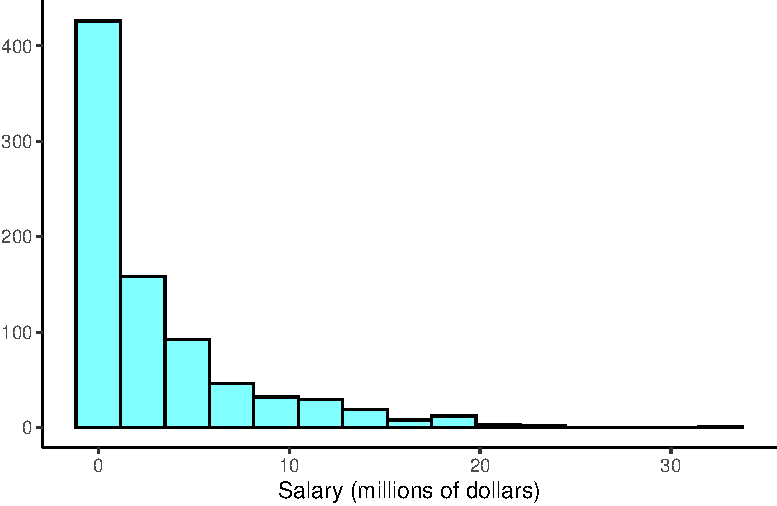
\includegraphics{Numerical-Data_files/figure-pdf/fig-hist510-1.pdf}

}

\caption{\label{fig-hist510}Histogram of MLB player salaries for 2010,
in millions of dollars.}

\end{figure}%

\begin{quote}
\emph{Example}:\\
The histogram of MLB player salaries is somewhat useful because we can
see that the data are extremely skewed and centered (as gauged by the
median) at about \$1 million. What about this plot is not
useful?\footnote{Most of the data are collected into one bin in the
  histogram and the data are so strongly skewed that many details in the
  data are obscured.}
\end{quote}

There are some standard transformations that are often applied when much
of the data cluster near zero (relative to the larger values in the data
set) and all observations are positive. A \textbf{transformation} is a
rescaling of the data using a function. For instance, a plot of the
natural logarithm\footnote{Statisticians often write the natural
  logarithm as \(\log\). You might be more familiar with it being
  written as \(\ln\).} of player salaries results in a new histogram in
Figure~\ref{fig-hist512}. Transformed data are sometimes easier to work
with when applying statistical models because the transformed data are
much less skewed and outliers are usually less extreme.

\begin{figure}

\centering{

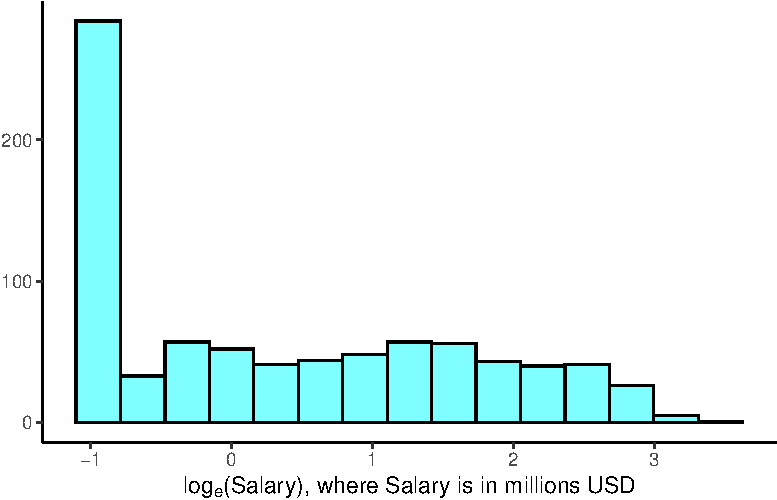
\includegraphics{Numerical-Data_files/figure-pdf/fig-hist512-1.pdf}

}

\caption{\label{fig-hist512}Histogram of the log-transformed MLB player
salaries for 2010.}

\end{figure}%

Transformations can also be applied to one or both variables in a
scatterplot. A scatterplot of the original \texttt{line\_breaks} and
\texttt{num\_char} variables is shown in Figure~\ref{fig-scat52} above.
We can see a positive association between the variables and that many
observations are clustered near zero. Later in this text, we might want
to use a straight line to model the data. However, we'll find that the
data in their current state cannot be modeled very well.
Figure~\ref{fig-scat513} shows a scatterplot where both
\texttt{line\_breaks} and \texttt{num\_char} have been transformed using
a natural log (log base \(e\)) transformation. While there is a positive
association in each plot, the transformed data show a steadier trend,
which is easier to model than the original (un-transformed) data.

\begin{figure}

\centering{

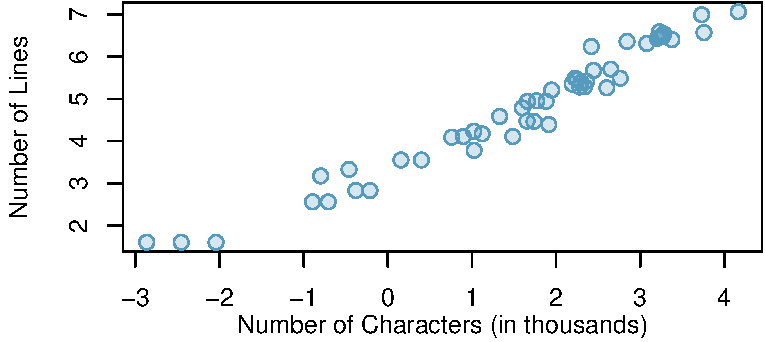
\includegraphics{Numerical-Data_files/figure-pdf/fig-scat513-1.pdf}

}

\caption{\label{fig-scat513}A scatterplot of \texttt{line\_breaks}
versus \texttt{num\_char} for the \texttt{email50} data, where both
variables have been log-transformed.}

\end{figure}%

Transformations other than the logarithm can be useful, too. For
instance, the square root (\(\sqrt{\text{original observation}}\)) and
inverse \(\left(\frac{1}{\text{original observation}}\right)\) are used
commonly by statisticians. Common goals in transforming data are to see
the data structure differently, reduce skew, assist in modeling, or
straighten a nonlinear relationship in a scatterplot.

\chapter{Categorical Data}\label{sec-CATDATA}

\section{Objectives}\label{objectives-6}

\begin{enumerate}
\def\labelenumi{\arabic{enumi})}
\item
  Differentiate between various statistical terminologies such as
  \emph{factor, contingency table, marginal counts, joint counts,
  frequency table, relative frequency table, bar plot, conditioning,
  segmented bar plot, mosaic plot, pie chart, side-by-side box plot,}
  and \emph{density plot}, and construct examples to demonstrate their
  proper use in context.
\item
  Using \texttt{R}, generate and interpret tables for categorical
  variables.
\item
  Using \texttt{R}, generate and interpret summary statistics for
  numerical variables by groups.
\item
  Create and evaluate graphical summaries of both categorical and
  numerical variables using \texttt{R}, selecting the most appropriate
  visualization techniques for different types of data and research
  questions.
\item
  Synthesize numerical and graphical summaries to provide
  interpretations and explanations of a data set.
\end{enumerate}

\section{Categorical data}\label{categorical-data-1}

Like numerical data, categorical data can also be organized and
analyzed. This section introduces tables and other basic tools for use
with categorical data. Remember at the beginning of this block of
material, our case study had categorical data so we have already seen
some of the ideas in this chapter.

The \texttt{email50} data set represents a sample from a larger email
data set called \texttt{email}. This larger data set contains
information on 3,921 emails. In this section, we will use the
\texttt{email} data set to examine whether the presence of numbers,
small or large, in an email provides any useful information in
classifying email as spam or not spam.

\subsection{Contingency tables and bar
plots}\label{contingency-tables-and-bar-plots}

In the \texttt{email} data set, we have two variables, \texttt{spam} and
\texttt{number}, that we want to summarize. Let's use \texttt{inspect()}
to get information and insight about the two variables. We can also type
\texttt{?email} or \texttt{help(email)} to learn more about the data.
First, load the \texttt{openintro} library.

\begin{Shaded}
\begin{Highlighting}[]
\FunctionTok{library}\NormalTok{(openintro)}
\end{Highlighting}
\end{Shaded}

\begin{Shaded}
\begin{Highlighting}[]
\NormalTok{email }\SpecialCharTok{\%\textgreater{}\%}
  \FunctionTok{select}\NormalTok{(spam, number) }\SpecialCharTok{\%\textgreater{}\%}
  \FunctionTok{inspect}\NormalTok{()}
\end{Highlighting}
\end{Shaded}

\begin{verbatim}

categorical variables:  
    name  class levels    n missing
1 number factor      3 3921       0
                                   distribution
1 small (72.1%), none (14%) ...                

quantitative variables:  
  name   class min Q1 median Q3 max       mean        sd    n missing
1 spam numeric   0  0      0  0   1 0.09359857 0.2913066 3921       0
\end{verbatim}

Notice the use of the \texttt{pipe} operator and how it adds to the ease
of reading the code. The \texttt{select()} function allows us to narrow
down the columns/variables to the two of interest. Then
\texttt{inspect()} gives us information about those variables. We read
from top line; we start with the data set \texttt{email}, input it into
\texttt{select()} and select variables from it, and then use
\texttt{inspect()} to summarize the variables.

As indicated above, \texttt{number} is a categorical variable (a
\emph{factor}) that describes whether an email contains no numbers, only
small numbers (values under 1 million), or at least one big number (a
value of 1 million or more). The variable \texttt{spam} is a numeric
variable, where \texttt{1} indicates the email is spam and \texttt{0}
indicates the email is not spam. To treat \texttt{spam} as categorical,
we will want to change it to a \emph{factor}, but first we will build a
table that summarizes data for the two variables
(Table~\ref{tbl-contin1}). This table is called a \textbf{contingency
table}\footnote{A contingency table is a two-way table that shows the
  distribution of one variable in rows and a second variable in columns.}.
Each value in the table represents the number of times a particular
combination of variable outcomes occurred.

\begin{longtable}[t]{lrrrr}

\caption{\label{tbl-contin1}A contingency table for the \texttt{email}
data.}

\tabularnewline

\\
\toprule
\multicolumn{1}{c}{Spam} & \multicolumn{3}{c}{Number} & \multicolumn{1}{c}{ } \\
\cmidrule(l{3pt}r{3pt}){1-1} \cmidrule(l{3pt}r{3pt}){2-4}
 & none & small & big & Total\\
\midrule
0 & 400 & 2659 & 495 & 3554\\
1 & 149 & 168 & 50 & 367\\
Total & 549 & 2827 & 545 & 3921\\
\bottomrule

\end{longtable}

Below is the \texttt{R} code to generate the contingency table.

\begin{Shaded}
\begin{Highlighting}[]
\FunctionTok{tally}\NormalTok{(}\SpecialCharTok{\textasciitilde{}}\NormalTok{spam }\SpecialCharTok{+}\NormalTok{ number, }\AttributeTok{data =}\NormalTok{ email, }\AttributeTok{margins =} \ConstantTok{TRUE}\NormalTok{)}
\end{Highlighting}
\end{Shaded}

\begin{verbatim}
       number
spam    none small  big Total
  0      400  2659  495  3554
  1      149   168   50   367
  Total  549  2827  545  3921
\end{verbatim}

The value 149 corresponds to the number of emails in the data set that
are spam \emph{and} had no numbers listed in the email. Row and column
totals are also included. The \textbf{row totals} provide the total
counts across each row (e.g.~\(149 + 168 + 50 = 367\)), and
\textbf{column totals} are total counts down each column. The row and
column totals are known as \textbf{marginal}\footnote{Marginal counts
  are counts based on only one of the variables in a contingency table.
  For example, there are 367 spam emails in the table.} counts (hence,
\texttt{margins\ =\ TRUE}) and the values in the table are known as
\textbf{joint}\footnote{Joint counts are counts based on both variables
  in a contingency table. For example, there are 149 emails that are
  spam \emph{and} contain no numbers.} counts.

Let's turn \texttt{spam} into a factor and update the \texttt{email}
data object. We will use \texttt{mutate()} to do this.

\begin{Shaded}
\begin{Highlighting}[]
\NormalTok{email }\OtherTok{\textless{}{-}}\NormalTok{ email }\SpecialCharTok{\%\textgreater{}\%}
  \FunctionTok{mutate}\NormalTok{(}\AttributeTok{spam =} \FunctionTok{factor}\NormalTok{(email}\SpecialCharTok{$}\NormalTok{spam, }\AttributeTok{levels =} \FunctionTok{c}\NormalTok{(}\DecValTok{1}\NormalTok{, }\DecValTok{0}\NormalTok{), }
                       \AttributeTok{labels =} \FunctionTok{c}\NormalTok{(}\StringTok{"spam"}\NormalTok{, }\StringTok{"not spam"}\NormalTok{)))}
\end{Highlighting}
\end{Shaded}

Now, let's check the data again.

\begin{Shaded}
\begin{Highlighting}[]
\NormalTok{email }\SpecialCharTok{\%\textgreater{}\%}
  \FunctionTok{select}\NormalTok{(spam, number) }\SpecialCharTok{\%\textgreater{}\%}
  \FunctionTok{inspect}\NormalTok{()}
\end{Highlighting}
\end{Shaded}

\begin{verbatim}

categorical variables:  
    name  class levels    n missing
1   spam factor      2 3921       0
2 number factor      3 3921       0
                                   distribution
1 not spam (90.6%), spam (9.4%)                
2 small (72.1%), none (14%) ...                
\end{verbatim}

Let's generate the contingency table again.

\begin{Shaded}
\begin{Highlighting}[]
\FunctionTok{tally}\NormalTok{(}\SpecialCharTok{\textasciitilde{}}\NormalTok{spam }\SpecialCharTok{+}\NormalTok{ number, }\AttributeTok{data =}\NormalTok{ email, }\AttributeTok{margins =} \ConstantTok{TRUE}\NormalTok{)}
\end{Highlighting}
\end{Shaded}

\begin{verbatim}
          number
spam       none small  big Total
  spam      149   168   50   367
  not spam  400  2659  495  3554
  Total     549  2827  545  3921
\end{verbatim}

A table for a single variable is called a \textbf{frequency table}. The
table below is a frequency table for the \texttt{number} variable.

\begin{Shaded}
\begin{Highlighting}[]
\FunctionTok{tally}\NormalTok{(}\SpecialCharTok{\textasciitilde{}}\NormalTok{number, }\AttributeTok{data =}\NormalTok{ email)}
\end{Highlighting}
\end{Shaded}

\begin{verbatim}
number
 none small   big 
  549  2827   545 
\end{verbatim}

If we replaced the counts with percentages or proportions, the table
would be called a \textbf{relative frequency table}.

\begin{Shaded}
\begin{Highlighting}[]
\FunctionTok{tally}\NormalTok{(}\SpecialCharTok{\textasciitilde{}}\NormalTok{number, }\AttributeTok{data =}\NormalTok{ email, }\AttributeTok{format =} \StringTok{\textquotesingle{}proportion\textquotesingle{}}\NormalTok{)}
\end{Highlighting}
\end{Shaded}

\begin{verbatim}
number
     none     small       big 
0.1400153 0.7209895 0.1389952 
\end{verbatim}

\begin{Shaded}
\begin{Highlighting}[]
\FunctionTok{round}\NormalTok{(}\FunctionTok{tally}\NormalTok{(}\SpecialCharTok{\textasciitilde{}}\NormalTok{number, }\AttributeTok{data =}\NormalTok{ email, }\AttributeTok{format =} \StringTok{\textquotesingle{}percent\textquotesingle{}}\NormalTok{), }\DecValTok{2}\NormalTok{)}
\end{Highlighting}
\end{Shaded}

\begin{verbatim}
number
 none small   big 
 14.0  72.1  13.9 
\end{verbatim}

A bar plot is a common way to display a single categorical variable.
Figure~\ref{fig-bar61} shows a \textbf{bar plot} for the \texttt{number}
variable.

\begin{Shaded}
\begin{Highlighting}[]
\NormalTok{email }\SpecialCharTok{\%\textgreater{}\%}
  \FunctionTok{gf\_bar}\NormalTok{(}\SpecialCharTok{\textasciitilde{}}\NormalTok{number) }\SpecialCharTok{\%\textgreater{}\%}
  \FunctionTok{gf\_theme}\NormalTok{(}\FunctionTok{theme\_bw}\NormalTok{()) }\SpecialCharTok{\%\textgreater{}\%}
  \FunctionTok{gf\_labs}\NormalTok{(}\AttributeTok{x =} \StringTok{"Size of Number"}\NormalTok{, }\AttributeTok{y =} \StringTok{"Count"}\NormalTok{)}
\end{Highlighting}
\end{Shaded}

\begin{figure}[H]

\centering{

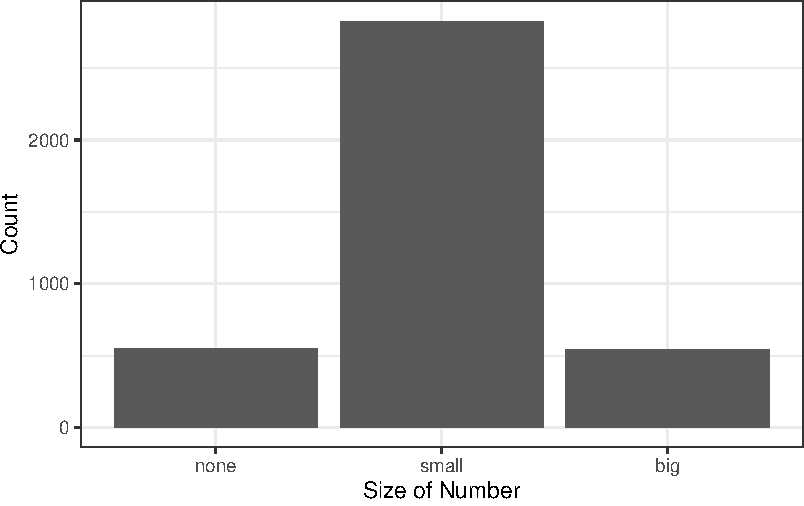
\includegraphics{Categorical-Data_files/figure-pdf/fig-bar61-1.pdf}

}

\caption{\label{fig-bar61}Bar chart of the \texttt{number} variable.}

\end{figure}%

Next, the counts are converted into proportions (e.g.,
\(549 / 3921 = 0.140\) for \texttt{none}) in Figure~\ref{fig-bar62}.

\begin{Shaded}
\begin{Highlighting}[]
\NormalTok{email }\SpecialCharTok{\%\textgreater{}\%}
  \FunctionTok{gf\_props}\NormalTok{(}\SpecialCharTok{\textasciitilde{}}\NormalTok{number) }\SpecialCharTok{\%\textgreater{}\%}
  \FunctionTok{gf\_theme}\NormalTok{(}\FunctionTok{theme\_bw}\NormalTok{()) }\SpecialCharTok{\%\textgreater{}\%}
  \FunctionTok{gf\_labs}\NormalTok{(}\AttributeTok{x =} \StringTok{"Size of Number"}\NormalTok{, }\AttributeTok{y =} \StringTok{"Proportion"}\NormalTok{)}
\end{Highlighting}
\end{Shaded}

\begin{figure}[H]

\centering{

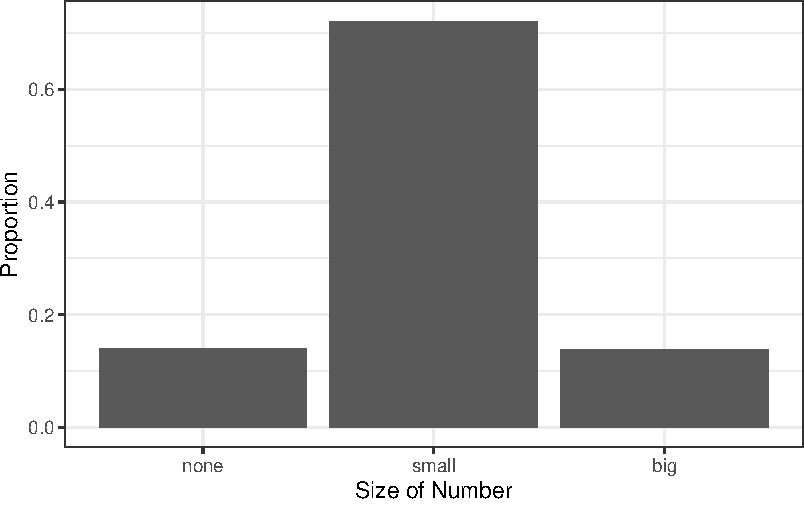
\includegraphics{Categorical-Data_files/figure-pdf/fig-bar62-1.pdf}

}

\caption{\label{fig-bar62}Bar chart of the \texttt{number} variable as a
proportion.}

\end{figure}%

Again, let's clean up the plot into a style that we could use in a
report.

\begin{Shaded}
\begin{Highlighting}[]
\NormalTok{email }\SpecialCharTok{\%\textgreater{}\%}
  \FunctionTok{gf\_props}\NormalTok{(}\SpecialCharTok{\textasciitilde{}}\NormalTok{number, }
           \AttributeTok{title =} \StringTok{"The proportions of emails with a number in it"}\NormalTok{,}
           \AttributeTok{subtitle =} \StringTok{"From 2012"}\NormalTok{, }\AttributeTok{xlab =} \StringTok{"Type of number in the email"}\NormalTok{,}
           \AttributeTok{ylab =} \StringTok{"Proportion of emails"}\NormalTok{) }\SpecialCharTok{\%\textgreater{}\%}
  \FunctionTok{gf\_theme}\NormalTok{(}\FunctionTok{theme\_bw}\NormalTok{())}
\end{Highlighting}
\end{Shaded}

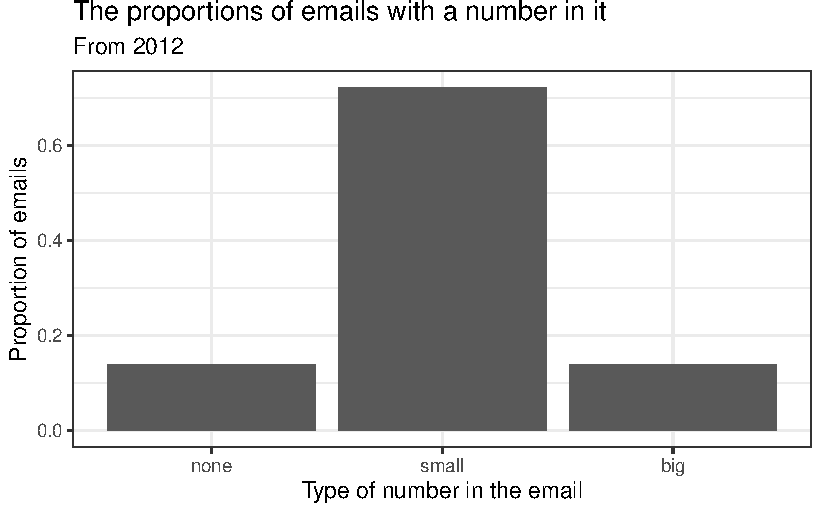
\includegraphics{Categorical-Data_files/figure-pdf/unnamed-chunk-16-1.pdf}

\subsection{Column proportions}\label{column-proportions}

The table below shows the column proportions. The \textbf{column
proportions} are computed as the counts divided by their column totals.
The value 149 at the intersection of \emph{spam} and \emph{none} is
replaced by \(149 / 549 = 0.271\), i.e., 149 divided by its column
total, 549. So what does 0.271 represent? It corresponds to the
proportion of emails in the sample with no numbers that are spam. That
is, the proportion of emails that are spam, out of all the emails with
no numbers. We are \textbf{conditioning}, restricting, on emails with no
number. This rate of spam is much higher than emails with only small
numbers (5.9\%) or big numbers (9.2\%). Because these spam rates vary
between the three levels of \texttt{number} (\emph{none}, \emph{small},
\emph{big}), this provides evidence that the \texttt{spam} and
\texttt{number} variables are associated.

\begin{Shaded}
\begin{Highlighting}[]
\FunctionTok{tally}\NormalTok{(spam }\SpecialCharTok{\textasciitilde{}}\NormalTok{ number, }\AttributeTok{data =}\NormalTok{ email, }\AttributeTok{margins =} \ConstantTok{TRUE}\NormalTok{, }\AttributeTok{format =} \StringTok{\textquotesingle{}proportion\textquotesingle{}}\NormalTok{)}
\end{Highlighting}
\end{Shaded}

\begin{verbatim}
          number
spam             none      small        big
  spam     0.27140255 0.05942695 0.09174312
  not spam 0.72859745 0.94057305 0.90825688
  Total    1.00000000 1.00000000 1.00000000
\end{verbatim}

The \texttt{tally()} function will always condition on the variable on
the right-hand side of the tilde, \textasciitilde, when calculating
proportions. Thus, \texttt{tally()} only generates column or overall
proportions. It cannot generate row proportions. The more general
\texttt{table()} function of \texttt{R} will allow either column or row
proportions.

\begin{quote}
\textbf{Exercise}:\\
Create a table of column proportions where the variable \texttt{spam} is
the column variable.
\end{quote}

\begin{Shaded}
\begin{Highlighting}[]
\FunctionTok{tally}\NormalTok{(number }\SpecialCharTok{\textasciitilde{}}\NormalTok{ spam, }\AttributeTok{data =}\NormalTok{ email, }\AttributeTok{margins =} \ConstantTok{TRUE}\NormalTok{, }\AttributeTok{format =} \StringTok{\textquotesingle{}proportion\textquotesingle{}}\NormalTok{)}
\end{Highlighting}
\end{Shaded}

\begin{verbatim}
       spam
number       spam  not spam
  none  0.4059946 0.1125492
  small 0.4577657 0.7481711
  big   0.1362398 0.1392797
  Total 1.0000000 1.0000000
\end{verbatim}

\begin{quote}
\textbf{Exercise}:\\
In the table you just created, what does 0.748 represent?\footnote{This
  is the proportion of \texttt{not\ spam} emails that had a small number
  in it.}
\end{quote}

\begin{quote}
\textbf{Exercise}: Create a table of proportions, where \texttt{spam} is
the column variable and the values shown represent the proportion of the
entire sample in each category.
\end{quote}

\begin{Shaded}
\begin{Highlighting}[]
\FunctionTok{tally}\NormalTok{(}\SpecialCharTok{\textasciitilde{}}\NormalTok{ number }\SpecialCharTok{+}\NormalTok{ spam, }\AttributeTok{data =}\NormalTok{ email, }\AttributeTok{margins =} \ConstantTok{TRUE}\NormalTok{, }\AttributeTok{format =} \StringTok{"proportion"}\NormalTok{)}
\end{Highlighting}
\end{Shaded}

\begin{verbatim}
       spam
number        spam   not spam      Total
  none  0.03800051 0.10201479 0.14001530
  small 0.04284621 0.67814333 0.72098954
  big   0.01275185 0.12624331 0.13899515
  Total 0.09359857 0.90640143 1.00000000
\end{verbatim}

\begin{quote}
\emph{Example}:\\
Data scientists use statistics to filter spam from incoming email
messages. By noting specific characteristics of an email, a data
scientist may be able to classify some emails as spam or not spam with
high accuracy. One of those characteristics is whether the email
contains no numbers, small numbers, or big numbers. Another
characteristic is whether or not an email has any HTML content (given by
the \texttt{format} variable). A contingency table for the \texttt{spam}
and \texttt{format} variables is needed.\\
1. Make \texttt{format} into a categorical factor variable. The levels
should be ``text'' and ``HTML''.\footnote{From the help menu on the
  data, HTML is coded as a 1.}\\
2. Create a contingency table from the \texttt{email} data set with
\texttt{format} in the columns and \texttt{spam} in the rows.
\end{quote}

\begin{Shaded}
\begin{Highlighting}[]
\NormalTok{email }\OtherTok{\textless{}{-}}\NormalTok{ email }\SpecialCharTok{\%\textgreater{}\%} 
  \FunctionTok{mutate}\NormalTok{(}\AttributeTok{format =} \FunctionTok{factor}\NormalTok{(email}\SpecialCharTok{$}\NormalTok{format, }\AttributeTok{levels =} \FunctionTok{c}\NormalTok{(}\DecValTok{1}\NormalTok{, }\DecValTok{0}\NormalTok{), }
                         \AttributeTok{labels =} \FunctionTok{c}\NormalTok{(}\StringTok{"HTML"}\NormalTok{, }\StringTok{"text"}\NormalTok{)))}
\end{Highlighting}
\end{Shaded}

In deciding which variable to use as a column, the data scientist would
be interested in how the proportion of spam changes within each email
format. This corresponds to column proportions based on \texttt{format}:
the proportion of spam in plain text emails and the proportion of spam
in HTML emails.

\begin{Shaded}
\begin{Highlighting}[]
\FunctionTok{tally}\NormalTok{(spam }\SpecialCharTok{\textasciitilde{}}\NormalTok{ format, }\AttributeTok{data =}\NormalTok{ email, }\AttributeTok{margins =} \ConstantTok{TRUE}\NormalTok{, }\AttributeTok{format =} \StringTok{"proportion"}\NormalTok{)}
\end{Highlighting}
\end{Shaded}

\begin{verbatim}
          format
spam             HTML       text
  spam     0.05796038 0.17489540
  not spam 0.94203962 0.82510460
  Total    1.00000000 1.00000000
\end{verbatim}

In generating the column proportions, we can see that a higher fraction
of plain text emails are spam (\(209 / 1195 = 17.5\%\)) compared to HTML
emails (\(158 / 2726 = 5.8\%\)). This information on its own is
insufficient to classify an email as spam or not spam, as over 80\% of
plain text emails are not spam. Yet, when we carefully combine this
information with many other characteristics, such as \texttt{number} and
other variables, we stand a reasonable chance of being able to classify
an email as spam or not spam.

In constructing a table, we need to think about which variable we want
in the column and which in the row. The formula notation in some ways
makes us think about the response and predictor variables, with the
response variable (left-hand side) displayed in the rows and the
predictor variable (right-hand side) displayed in the columns. However,
in some cases, it is not clear which variable should be in the column
and row and the analyst must decide what is being communicated with the
table. Before settling on one form for a table, it is important to
consider the audience and the message they are to receive from the
table.

\begin{quote}
\textbf{Exercise}:\\
Create two tables with \texttt{number} and \texttt{spam}: one where
\texttt{number} is in the columns, and one where \texttt{spam} is in the
columns. Which table would be more useful to someone hoping to identify
spam emails based on the type of numbers in the email?\footnote{The
  table with \texttt{number} in the columns will probably be most
  useful. This table makes it easier to see that emails with small
  numbers are spam about 5.9\% of the time (relatively rare). In
  contrast, we see that about 27.1\% of emails with no numbers are spam,
  and 9.2\% of emails with big numbers are spam.}
\end{quote}

\begin{Shaded}
\begin{Highlighting}[]
\FunctionTok{tally}\NormalTok{(spam }\SpecialCharTok{\textasciitilde{}}\NormalTok{ number, }\AttributeTok{data =}\NormalTok{ email, }\AttributeTok{format =} \StringTok{\textquotesingle{}proportion\textquotesingle{}}\NormalTok{, }\AttributeTok{margin =} \ConstantTok{TRUE}\NormalTok{)}
\end{Highlighting}
\end{Shaded}

\begin{verbatim}
          number
spam             none      small        big
  spam     0.27140255 0.05942695 0.09174312
  not spam 0.72859745 0.94057305 0.90825688
  Total    1.00000000 1.00000000 1.00000000
\end{verbatim}

\begin{Shaded}
\begin{Highlighting}[]
\FunctionTok{tally}\NormalTok{(number }\SpecialCharTok{\textasciitilde{}}\NormalTok{ spam, }\AttributeTok{data =}\NormalTok{ email, }\AttributeTok{format =} \StringTok{\textquotesingle{}proportion\textquotesingle{}}\NormalTok{, }\AttributeTok{margin =} \ConstantTok{TRUE}\NormalTok{)}
\end{Highlighting}
\end{Shaded}

\begin{verbatim}
       spam
number       spam  not spam
  none  0.4059946 0.1125492
  small 0.4577657 0.7481711
  big   0.1362398 0.1392797
  Total 1.0000000 1.0000000
\end{verbatim}

\subsection{Segmented bar and mosaic
plots}\label{segmented-bar-and-mosaic-plots}

Contingency tables using column proportions are especially useful for
examining how two categorical variables are related. Segmented bar and
mosaic plots provide a way to visualize the information in these tables.

A \textbf{segmented bar plot} is a graphical display of contingency
table information. For example, a segmented bar plot representing the
table with \texttt{number} in the columns is shown in
Figure~\ref{fig-barseg61}, where we have first created a bar plot using
the \texttt{number} variable and then separated each group by the levels
of \texttt{spam} using the \texttt{fill} argument.

\begin{Shaded}
\begin{Highlighting}[]
\NormalTok{email }\SpecialCharTok{\%\textgreater{}\%}
  \FunctionTok{gf\_bar}\NormalTok{(}\SpecialCharTok{\textasciitilde{}}\NormalTok{number, }\AttributeTok{fill =} \SpecialCharTok{\textasciitilde{}}\NormalTok{spam) }\SpecialCharTok{\%\textgreater{}\%}
  \FunctionTok{gf\_theme}\NormalTok{(}\FunctionTok{theme\_bw}\NormalTok{()) }\SpecialCharTok{\%\textgreater{}\%}
  \FunctionTok{gf\_labs}\NormalTok{(}\AttributeTok{x =} \StringTok{"Size of Number"}\NormalTok{, }\AttributeTok{y =} \StringTok{"Count"}\NormalTok{)}
\end{Highlighting}
\end{Shaded}

\begin{figure}[H]

\centering{

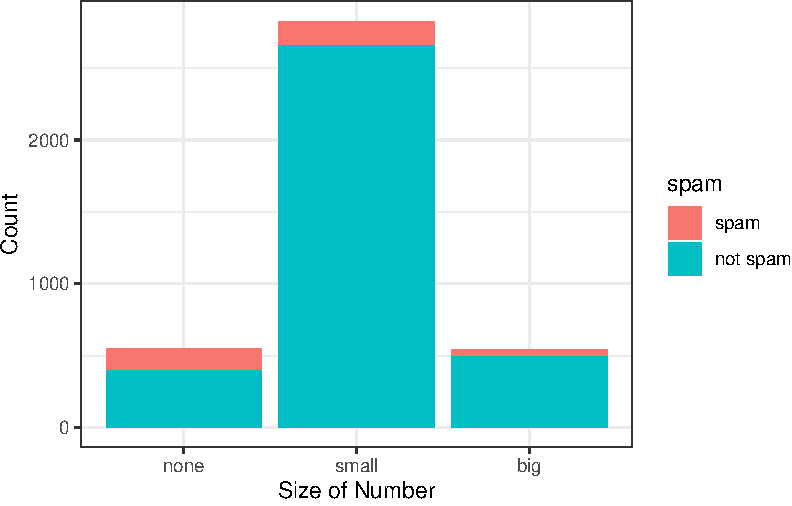
\includegraphics{Categorical-Data_files/figure-pdf/fig-barseg61-1.pdf}

}

\caption{\label{fig-barseg61}Segmented bar plot for numbers found in
\texttt{emails}, where the counts have been further broken down by
\texttt{spam}.}

\end{figure}%

The column proportions of the table have been translated into a
standardized segmented bar plot in Figure~\ref{fig-barseg62}, which is a
helpful visualization of the fraction of spam emails within each level
of \texttt{number}.

\begin{Shaded}
\begin{Highlighting}[]
\NormalTok{email }\SpecialCharTok{\%\textgreater{}\%}
  \FunctionTok{gf\_props}\NormalTok{(}\SpecialCharTok{\textasciitilde{}}\NormalTok{number, }\AttributeTok{fill =} \SpecialCharTok{\textasciitilde{}}\NormalTok{spam, }\AttributeTok{position =} \StringTok{\textquotesingle{}fill\textquotesingle{}}\NormalTok{) }\SpecialCharTok{\%\textgreater{}\%}
  \FunctionTok{gf\_theme}\NormalTok{(}\FunctionTok{theme\_bw}\NormalTok{()) }\SpecialCharTok{\%\textgreater{}\%}
  \FunctionTok{gf\_labs}\NormalTok{(}\AttributeTok{x =} \StringTok{"Size of Number"}\NormalTok{, }\AttributeTok{y =} \StringTok{"Proportion"}\NormalTok{)}
\end{Highlighting}
\end{Shaded}

\begin{figure}[H]

\centering{

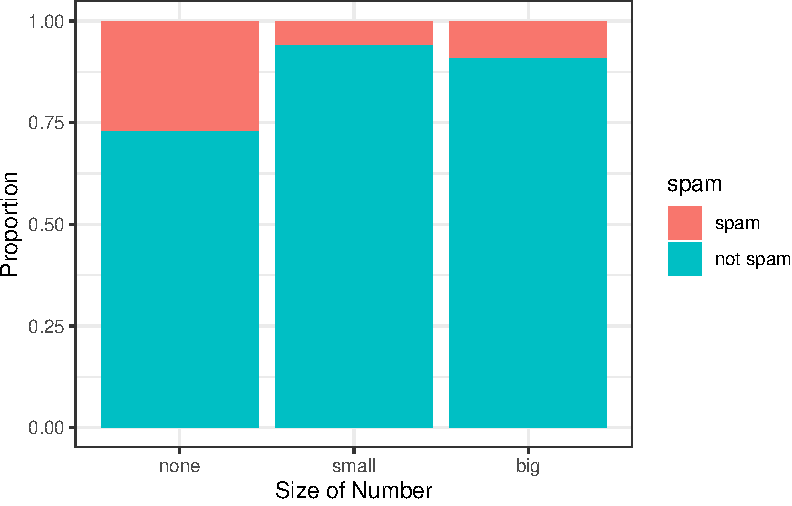
\includegraphics{Categorical-Data_files/figure-pdf/fig-barseg62-1.pdf}

}

\caption{\label{fig-barseg62}Standardized version of
Figure~\ref{fig-barseg61}.}

\end{figure}%

\begin{quote}
\emph{Example}:\\
Examine both of the segmented bar plots. Which is more
useful?\footnote{Figure~\ref{fig-barseg61} contains more information,
  but Figure~\ref{fig-barseg62} presents the information more clearly.
  This second plot makes it clear that emails with no number have a
  relatively high rate of spam email -- about 27\%! On the other hand,
  less than 10\% of emails with small or big numbers are spam.}
\end{quote}

Since the proportion of spam changes across the groups in
Figure~\ref{fig-barseg62}, we can conclude the variables are dependent,
which is something we were also able to discern using table proportions.
Because both the \texttt{none} and \texttt{big} groups have relatively
few observations compared to the \texttt{small} group, the association
is more difficult to see in Figure~\ref{fig-barseg61}.

In other cases, a segmented bar plot that is not standardized will be
more useful in communicating important information. Before settling on a
particular segmented bar plot, create standardized and non-standardized
forms and decide which is more effective at communicating features of
the data.

A \textbf{mosaic plot} is a graphical display of contingency table
information that is similar to a bar plot for one variable or a
segmented bar plot when using two variables. It seems strange, but
mosaic plots are not part of the \textbf{mosaic} package. We must load
another set of packages called \textbf{vcd} and \textbf{vcdExtra}.
Mosaic plots help to visualize the pattern of associations among
variables in two-way and larger tables. Mosaic plots are controversial
because they rely on the perception of area; human vision is not good at
distinguishing areas.

We introduce mosaic plots as another way to visualize contingency
tables. Figure~\ref{fig-mosaic61} shows a one-variable mosaic plot for
the \texttt{number} variable. Each row represents a level of
\texttt{number}, and the row heights correspond to the proportion of
emails of each number type. For instance, there are fewer emails with no
numbers than emails with only small numbers, so the \texttt{none}
outcome row is shorter in height. In general, mosaic plots use box
\emph{areas} to represent the number of observations. Since there is
only one variable, the widths are all constant. Thus area is simply
related to row height making this visual easy to read.

\begin{Shaded}
\begin{Highlighting}[]
\FunctionTok{library}\NormalTok{(vcd)}
\end{Highlighting}
\end{Shaded}

\begin{Shaded}
\begin{Highlighting}[]
\FunctionTok{mosaic}\NormalTok{(}\SpecialCharTok{\textasciitilde{}}\NormalTok{number, }\AttributeTok{data =}\NormalTok{ email)}
\end{Highlighting}
\end{Shaded}

\begin{figure}[H]

\centering{

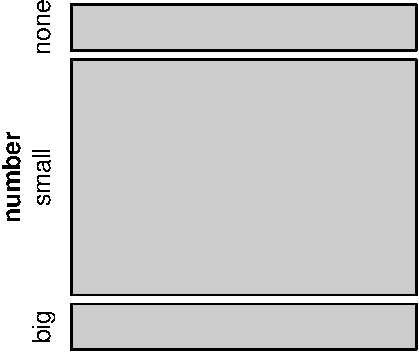
\includegraphics{Categorical-Data_files/figure-pdf/fig-mosaic61-1.pdf}

}

\caption{\label{fig-mosaic61}Mosaic plot where emails are grouped by the
\texttt{number} variable.}

\end{figure}%

This one-variable mosaic plot can be further divided into pieces as in
Figure~\ref{fig-mosaic62} using the \texttt{spam} variable. The first
variable in the formula is used to determine row height. That is, each
row is split proportionally according to the fraction of emails in each
number category. These heights are similar to those in
Figure~\ref{fig-mosaic61}. Next, each row is split horizontally
according to the proportion of emails that were spam in that number
group. For example, the second row, representing emails with only small
numbers, was divided into emails that were spam (left) and not spam
(right). The area of the rectangles represents the overall proportions
in the table, where each cell count is divided by the total count.
First, we will generate the table and then represent it as a mosaic
plot.

\begin{Shaded}
\begin{Highlighting}[]
\FunctionTok{tally}\NormalTok{(}\SpecialCharTok{\textasciitilde{}}\NormalTok{number }\SpecialCharTok{+}\NormalTok{ spam, }\AttributeTok{data =}\NormalTok{ email, }\AttributeTok{format =} \StringTok{\textquotesingle{}proportion\textquotesingle{}}\NormalTok{)}
\end{Highlighting}
\end{Shaded}

\begin{verbatim}
       spam
number        spam   not spam
  none  0.03800051 0.10201479
  small 0.04284621 0.67814333
  big   0.01275185 0.12624331
\end{verbatim}

\begin{Shaded}
\begin{Highlighting}[]
\FunctionTok{mosaic}\NormalTok{(}\SpecialCharTok{\textasciitilde{}}\NormalTok{number }\SpecialCharTok{+}\NormalTok{ spam, }\AttributeTok{data =}\NormalTok{ email)}
\end{Highlighting}
\end{Shaded}

\begin{figure}[H]

\centering{

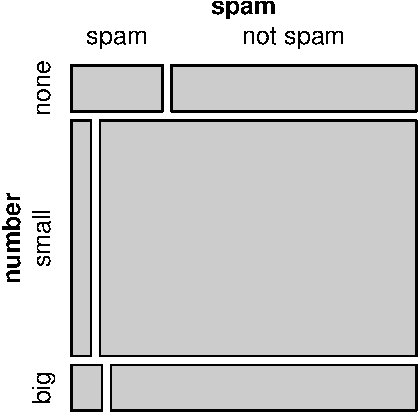
\includegraphics{Categorical-Data_files/figure-pdf/fig-mosaic62-1.pdf}

}

\caption{\label{fig-mosaic62}Mosaic plot with \texttt{number} as the
first (row) variable.}

\end{figure}%

These plots are hard to use in a visual comparison of area. For example,
is the area for \emph{small} number \emph{spam} emails different from
\emph{none} number \emph{spam} emails? The rectangles have different
shapes but from the table we can tell the areas are very similar.

An important use of the mosaic plot is to determine if an association
between variables may be present. The bottom row of the first column
represents spam emails that had big numbers, and the bottom row of the
second column represents regular emails that had big numbers. We can
again use this plot to see that the \texttt{spam} and \texttt{number}
variables are associated since some rows are divided in different
vertical locations than others, which was the same technique used for
checking an association in the standardized version of the segmented bar
plot.

In a similar way, a mosaic plot representing column proportions where
\emph{spam} is in the column could be constructed.

\begin{Shaded}
\begin{Highlighting}[]
\FunctionTok{mosaic}\NormalTok{(}\SpecialCharTok{\textasciitilde{}}\NormalTok{spam }\SpecialCharTok{+}\NormalTok{ number, }\AttributeTok{data =}\NormalTok{ email)}
\end{Highlighting}
\end{Shaded}

\begin{figure}[H]

\centering{

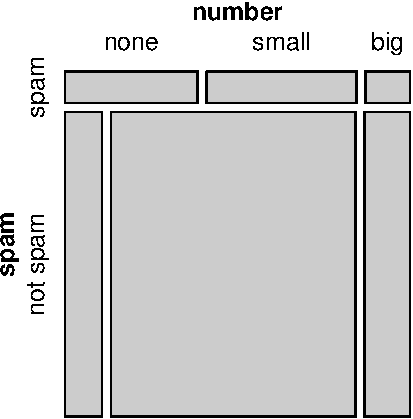
\includegraphics{Categorical-Data_files/figure-pdf/fig-mosaic63-1.pdf}

}

\caption{\label{fig-mosaic63}Mosaic plot with \texttt{spam} as the first
(row) variable.}

\end{figure}%

To completely understand the mosaic plot as shown in
Figure~\ref{fig-mosaic63}, let's first find the proportions of
\texttt{spam}.

\begin{Shaded}
\begin{Highlighting}[]
\FunctionTok{tally}\NormalTok{(}\SpecialCharTok{\textasciitilde{}}\NormalTok{spam, }\AttributeTok{data =}\NormalTok{ email, }\AttributeTok{format =} \StringTok{"proportion"}\NormalTok{)}
\end{Highlighting}
\end{Shaded}

\begin{verbatim}
spam
      spam   not spam 
0.09359857 0.90640143 
\end{verbatim}

So, the row heights will be split 90-10. Next, let's find the
proportions of \texttt{number} within each value of \texttt{spam}. In
the spam row, \emph{none} will be 41\%, \emph{small} will be 46\%, and
\emph{big} will be 13\%. In the not spam row, \emph{none} will be 11\%,
\emph{small} will be 75\%, and \emph{big} will be 14\%.

\begin{Shaded}
\begin{Highlighting}[]
\FunctionTok{tally}\NormalTok{(number }\SpecialCharTok{\textasciitilde{}}\NormalTok{ spam, }\AttributeTok{data =}\NormalTok{ email, }\AttributeTok{margins =} \ConstantTok{TRUE}\NormalTok{, }\AttributeTok{format =} \StringTok{"proportion"}\NormalTok{)}
\end{Highlighting}
\end{Shaded}

\begin{verbatim}
       spam
number       spam  not spam
  none  0.4059946 0.1125492
  small 0.4577657 0.7481711
  big   0.1362398 0.1392797
  Total 1.0000000 1.0000000
\end{verbatim}

However, because it is more insightful for this application to consider
the fraction of spam in each category of the \texttt{number} variable,
we prefer Figure~\ref{fig-mosaic62}.

\subsection{The only pie chart you will see in this book,
hopefully}\label{the-only-pie-chart-you-will-see-in-this-book-hopefully}

While pie charts are well known, they are typically not as useful as
other charts in a data analysis. A \textbf{pie chart} is shown in
Figure~\ref{fig-pie61}. It is generally more difficult to compare group
sizes in a pie chart than in a bar plot, especially when categories have
nearly identical counts or proportions. Just as human vision is bad at
distinguishing areas, human vision is also bad at distinguishing angles.
In the case of the \emph{none} and \emph{big} categories, the difference
is so slight you may be unable to distinguish any difference in group
sizes.

\begin{Shaded}
\begin{Highlighting}[]
\FunctionTok{pie}\NormalTok{(}\FunctionTok{table}\NormalTok{(email}\SpecialCharTok{$}\NormalTok{number), }\AttributeTok{col =}\NormalTok{ COL[}\FunctionTok{c}\NormalTok{(}\DecValTok{3}\NormalTok{, }\DecValTok{1}\NormalTok{, }\DecValTok{2}\NormalTok{)], }\AttributeTok{radius =} \FloatTok{0.75}\NormalTok{)}
\end{Highlighting}
\end{Shaded}

\begin{figure}[H]

\centering{

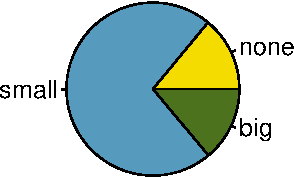
\includegraphics{Categorical-Data_files/figure-pdf/fig-pie61-1.pdf}

}

\caption{\label{fig-pie61}A pie chart for \texttt{number} in the email
data set.}

\end{figure}%

Pie charts are popular in the Air Force due to the ease of generating
them in Excel and PowerPoint. However, the values for each slice are
often printed on top of the chart making the chart irrelevant. We
recommend a minimal use of pie charts in your work.

\subsection{Comparing numerical data across
groups}\label{comparing-numerical-data-across-groups}

Some of the more interesting investigations can be done by examining
numerical data across groups. This is the case where one variable is
categorical and the other is numerical. The methods required here aren't
really new. All that is required is to make a numerical plot for each
group. Here, two convenient methods are introduced: side-by-side box
plots and density plots.

We will again take a look at the subset of the \texttt{county\_complete}
data set. Let's compare the median household income for counties that
gained population from 2000 to 2010 versus counties that had no gain.
While we might like to make a causal connection here, remember that
these are observational data, so such an interpretation would be
unjustified.

This section will give us a chance to perform some data wrangling. We
will be using the \texttt{tidyverse} verbs in the process. Data
wrangling is an important part of analysis work and typically makes up a
significant portion of the analysis work.

Here is the code to generate the data we need.

\begin{Shaded}
\begin{Highlighting}[]
\FunctionTok{library}\NormalTok{(usdata)}
\end{Highlighting}
\end{Shaded}

\begin{Shaded}
\begin{Highlighting}[]
\NormalTok{county\_tidy }\OtherTok{\textless{}{-}}\NormalTok{ county\_complete }\SpecialCharTok{\%\textgreater{}\%} 
  \FunctionTok{select}\NormalTok{(name, state, pop2000, pop2010, }\AttributeTok{fed\_spend =}\NormalTok{ fed\_spending\_2009, }
         \AttributeTok{poverty =}\NormalTok{ poverty\_2010, }\AttributeTok{homeownership =}\NormalTok{ homeownership\_2010, }
         \AttributeTok{multi\_unit =}\NormalTok{ housing\_multi\_unit\_2010, }\AttributeTok{income =}\NormalTok{ per\_capita\_income\_2010, }
         \AttributeTok{med\_income =}\NormalTok{ median\_household\_income\_2010) }\SpecialCharTok{\%\textgreater{}\%}
  \FunctionTok{mutate}\NormalTok{(}\AttributeTok{fed\_spend =}\NormalTok{ fed\_spend }\SpecialCharTok{/}\NormalTok{ pop2010)}
\end{Highlighting}
\end{Shaded}

First, as a reminder, let's look at the data.

\emph{What do we want \texttt{R} to do?}

We want to select the variables \texttt{pop2000}, \texttt{pop2010}, and
\texttt{med\_income}.

\emph{What does \texttt{R} need in order to do this?}

It needs the data object, and the desired variable names.

We will use the \texttt{select()} and \texttt{inspect()} functions.

\begin{Shaded}
\begin{Highlighting}[]
\NormalTok{county\_tidy }\SpecialCharTok{\%\textgreater{}\%}
  \FunctionTok{select}\NormalTok{(pop2000, pop2010, med\_income) }\SpecialCharTok{\%\textgreater{}\%}
  \FunctionTok{inspect}\NormalTok{()}
\end{Highlighting}
\end{Shaded}

\begin{verbatim}

quantitative variables:  
        name   class   min       Q1 median    Q3     max     mean        sd
1    pop2000 numeric    67 11223.50  24621 61775 9519338 89649.99 292547.67
2    pop2010 numeric    82 11114.50  25872 66780 9818605 98262.04 312946.70
3 med_income numeric 19351 36956.25  42450 49144  115574 44274.12  11547.49
     n missing
1 3139       3
2 3142       0
3 3142       0
\end{verbatim}

Notice that three counties are missing population values for the year
2000, reported as \texttt{NA}. Let's remove them and find which counties
increased in population by creating a new variable.

\begin{Shaded}
\begin{Highlighting}[]
\NormalTok{cc\_reduced }\OtherTok{\textless{}{-}}\NormalTok{ county\_tidy }\SpecialCharTok{\%\textgreater{}\%}
  \FunctionTok{drop\_na}\NormalTok{(pop2000) }\SpecialCharTok{\%\textgreater{}\%}
  \FunctionTok{select}\NormalTok{(pop2000, pop2010, med\_income) }\SpecialCharTok{\%\textgreater{}\%}
  \FunctionTok{mutate}\NormalTok{(}\AttributeTok{pop\_gain =} \FunctionTok{sign}\NormalTok{(pop2010}\SpecialCharTok{{-}}\NormalTok{pop2000))}
\end{Highlighting}
\end{Shaded}

\begin{Shaded}
\begin{Highlighting}[]
\FunctionTok{tally}\NormalTok{(}\SpecialCharTok{\textasciitilde{}}\NormalTok{pop\_gain, }\AttributeTok{data =}\NormalTok{ cc\_reduced)}
\end{Highlighting}
\end{Shaded}

\begin{verbatim}
pop_gain
  -1    0    1 
1097    1 2041 
\end{verbatim}

There were 2,041 counties where the population increased from 2000 to
2010, and there were 1,098 counties with no gain. Only 1 county had a
net of zero, and 1,0987 had a loss. Let's just look at the counties with
a gain or loss in a side-by-side boxplot. Again, we will use
\texttt{filter()} to select the two groups and then make the variable
\texttt{pop\_gain} into a categorical variable. It's time for more data
wrangling.

\begin{Shaded}
\begin{Highlighting}[]
\NormalTok{cc\_reduced }\OtherTok{\textless{}{-}}\NormalTok{ cc\_reduced }\SpecialCharTok{\%\textgreater{}\%}
  \FunctionTok{filter}\NormalTok{(pop\_gain }\SpecialCharTok{!=} \DecValTok{0}\NormalTok{) }\SpecialCharTok{\%\textgreater{}\%}
  \FunctionTok{mutate}\NormalTok{(}\AttributeTok{pop\_gain =} \FunctionTok{factor}\NormalTok{(pop\_gain, }\AttributeTok{levels =} \FunctionTok{c}\NormalTok{(}\SpecialCharTok{{-}}\DecValTok{1}\NormalTok{, }\DecValTok{1}\NormalTok{), }
                           \AttributeTok{labels =} \FunctionTok{c}\NormalTok{(}\StringTok{"Loss"}\NormalTok{, }\StringTok{"Gain"}\NormalTok{)))}
\end{Highlighting}
\end{Shaded}

\begin{Shaded}
\begin{Highlighting}[]
\FunctionTok{inspect}\NormalTok{(cc\_reduced)}
\end{Highlighting}
\end{Shaded}

\begin{verbatim}

categorical variables:  
      name  class levels    n missing
1 pop_gain factor      2 3138       0
                                   distribution
1 Gain (65%), Loss (35%)                       

quantitative variables:  
        name   class   min       Q1  median      Q3     max     mean        sd
1    pop2000 numeric    67 11217.25 24608.0 61783.5 9519338 89669.37 292592.28
2    pop2010 numeric    82 11127.00 25872.0 66972.0 9818605 98359.23 313133.28
3 med_income numeric 19351 36950.00 42443.5 49120.0  115574 44253.24  11528.95
     n missing
1 3138       0
2 3138       0
3 3138       0
\end{verbatim}

The \textbf{side-by-side box plot} is a traditional tool for comparing
across groups. An example is shown in Figure~\ref{fig-sbysbox61} where
there are two box plots, one for each group, drawn on the same scale.

\begin{Shaded}
\begin{Highlighting}[]
\NormalTok{cc\_reduced }\SpecialCharTok{\%\textgreater{}\%}
  \FunctionTok{gf\_boxplot}\NormalTok{(med\_income }\SpecialCharTok{\textasciitilde{}}\NormalTok{ pop\_gain,}
             \AttributeTok{subtitle =} \StringTok{"The income data were collected between 2006 and 2010."}\NormalTok{,}
             \AttributeTok{xlab =} \StringTok{"Population change from 2000 to 2010"}\NormalTok{,}
             \AttributeTok{ylab =} \StringTok{"Median Household Income"}\NormalTok{) }\SpecialCharTok{\%\textgreater{}\%}
  \FunctionTok{gf\_theme}\NormalTok{(}\FunctionTok{theme\_bw}\NormalTok{())}
\end{Highlighting}
\end{Shaded}

\begin{figure}[H]

\centering{

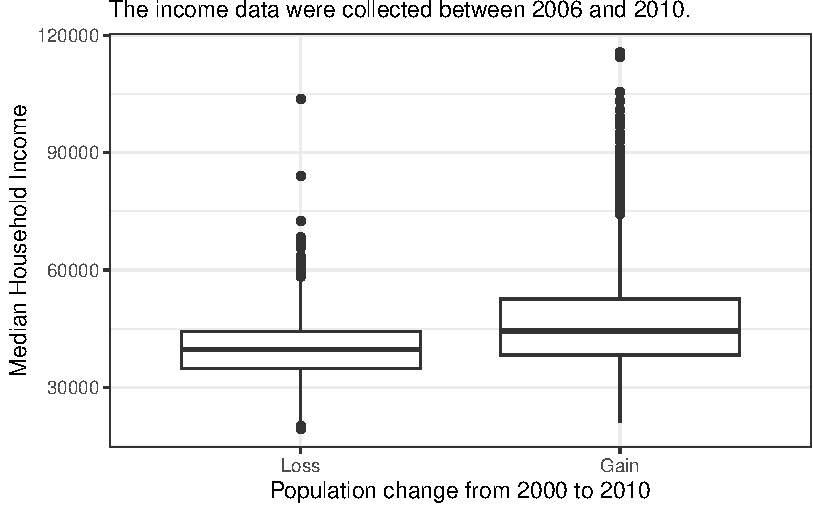
\includegraphics{Categorical-Data_files/figure-pdf/fig-sbysbox61-1.pdf}

}

\caption{\label{fig-sbysbox61}Side-by-side box plot for median household
income, where the counties are split by whether there was a population
gain or loss from 2000 to 2010.}

\end{figure}%

Figure~\ref{fig-dens61} is a plot of the two density curves as another
way of comparing median income by whether there was a population gain or
loss.

\begin{Shaded}
\begin{Highlighting}[]
\NormalTok{cc\_reduced }\SpecialCharTok{\%\textgreater{}\%}
  \FunctionTok{gf\_dens}\NormalTok{(}\SpecialCharTok{\textasciitilde{}}\NormalTok{med\_income, }\AttributeTok{color =} \SpecialCharTok{\textasciitilde{}}\NormalTok{pop\_gain, }\AttributeTok{lwd =} \DecValTok{1}\NormalTok{) }\SpecialCharTok{\%\textgreater{}\%}
  \FunctionTok{gf\_theme}\NormalTok{(}\FunctionTok{theme\_bw}\NormalTok{()) }\SpecialCharTok{\%\textgreater{}\%}
  \FunctionTok{gf\_labs}\NormalTok{(}\AttributeTok{x =} \StringTok{"Median household income"}\NormalTok{, }\AttributeTok{y =} \StringTok{"Density"}\NormalTok{, }\AttributeTok{col =} \StringTok{"Population }\SpecialCharTok{\textbackslash{}n}\StringTok{Change"}\NormalTok{)}
\end{Highlighting}
\end{Shaded}

\begin{figure}[H]

\centering{

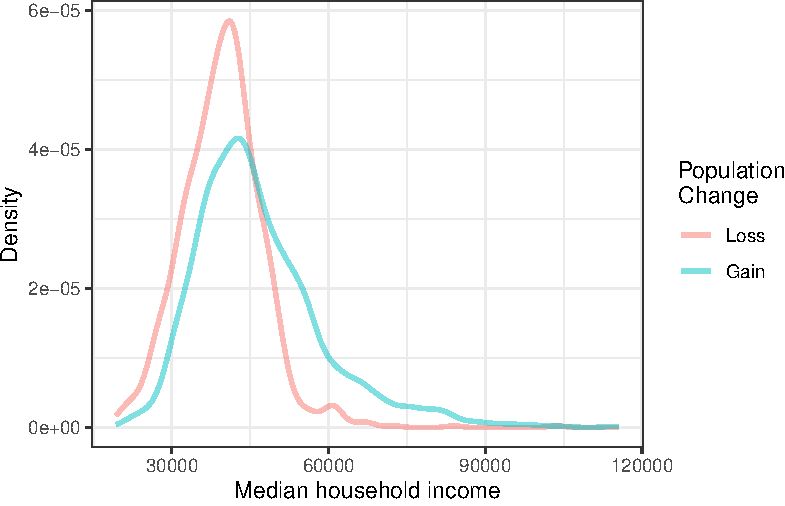
\includegraphics{Categorical-Data_files/figure-pdf/fig-dens61-1.pdf}

}

\caption{\label{fig-dens61}Density plots of median household income for
counties with population gain versus population loss.}

\end{figure}%

\begin{quote}
\textbf{Exercise}:\\
Use the box plots and density plots to compare the incomes for counties
across the two groups. What do you notice about the approximate center
of each group? What do you notice about the variability between groups?
Is the shape relatively consistent between groups? How many
\emph{prominent} modes are there for each group?\footnote{Answers may
  vary a little. The counties with population gains tend to have higher
  income (median of about \$45,000) versus counties without a gain
  (median of about \$40,000). The variability is also slightly larger
  for the population gain group. This is evident in the IQR, which is
  about 50\% bigger in the \emph{gain} group. Both distributions show
  slight to moderate right skew and are unimodal. There is a secondary
  small bump at about \$60,000 for the \emph{no gain} group, visible in
  the density plot, that seems out of place. (Looking into the data set,
  we would find that 8 of these 15 counties are in Alaska and Texas.)
  The box plots indicate there are many observations far above the
  median in each group, though we should anticipate that many
  observations will fall beyond the whiskers when using such a large
  data set.}
\end{quote}

\begin{quote}
\textbf{Exercise}:\\
What components of Figures~\ref{fig-sbysbox61}, \ref{fig-dens61} do you
find most useful?\footnote{The side-by-side box plots are especially
  useful for comparing centers and spreads, while the density plots are
  more useful for seeing distribution shape, skew, and groups of
  anomalies.}
\end{quote}

\part{Probability Modeling}

\chapter{Probability Case Study}\label{sec-CS2}

\section{Objectives}\label{objectives-7}

\begin{enumerate}
\def\labelenumi{\arabic{enumi})}
\item
  Use \texttt{R} to simulate a probabilistic model.
\item
  Gain an introduction to probabilistic thinking through computational,
  mathematical, and data science approaches.
\end{enumerate}

\section{Introduction to probability
models}\label{introduction-to-probability-models}

In this second block of material, we will focus on probability models.
We will provide both a mathematical approach and a computational
approach. We will focus on the latter and leave much of the mathematical
details to the interested learner. In some cases we can use both methods
on a problem and in others only the computational approach is feasible.
The mathematical approach to probability modeling allows us insight into
the problem and the ability to understand the process. The computational
approach has a much greater ability to generalize but can be time
intensive to run and often requires the writing of custom functions.

This case study is extensive and may seem overwhelming, but do not
worry. We will discuss these ideas again in the many chapters we have
coming up this block.

\section{Probability models}\label{probability-models}

Probability models are an important tool for data analysts. They are
used to explain variation in outcomes that cannot be explained by other
variables. We will use these ideas in the Statistical Modeling Block to
help us make decisions about our statistical models.

Often probability models are used to answer a question of the form
``What is the chance that \ldots..?'' This means that we typically have
an experiment or trial where multiple outcomes are possible and we only
have an idea of the frequency of those outcomes. We use this frequency
as a measure of the probability of a particular outcome.

For this block we will focus just on probability models. To apply a
probability model we will need to

\begin{enumerate}
\def\labelenumi{\arabic{enumi}.}
\tightlist
\item
  Describe the experiment and its possible outcomes.
\item
  Determine probability values for the outcomes, which may include
  \textbf{parameters} that determine the probabilities.
\item
  Understand the assumptions behind the model.
\end{enumerate}

\section{Case study}\label{case-study-1}

There is a famous example of a probability question that we will examine
in this case study. The question we want to answer is ``In a room of
\(n\) people, what is the chance at least two people have the same
birthday?''

\begin{quote}
\textbf{Exercise}:\\
The typical classroom at USAFA has 18 students in it. What do you think
is the chance that at least two students have the same
birthday?\footnote{The answer is around 34.7\%. How close were you? Did
  you think it was lower or higher?}
\end{quote}

\subsection{Break down the question}\label{break-down-the-question}

The first action we should take is to understand what is being asked.

\begin{enumerate}
\def\labelenumi{\arabic{enumi}.}
\tightlist
\item
  What is the experiment or trial?
\item
  What does it mean to have the same birthday?
\item
  How should we handle leap years?
\item
  Should we consider the frequency of births? Are some days less likely
  than others?
\end{enumerate}

\begin{quote}
\textbf{Exercise}:\\
Discuss these questions and others that you think are
relevant.\footnote{Another question may be ``What does it mean at least
  two people have matching birthdays?''}
\end{quote}

The best first step is to develop a simple model. Often these are the
only ones that will have a mathematical solution. For our problem this
means we answer the above questions.

\begin{enumerate}
\def\labelenumi{\arabic{enumi}.}
\tightlist
\item
  We have a room of 18 people and we look at their birthdays. We either
  have two or more birthdays matching or not; thus there are two
  outcomes.
\item
  At least two people having the same birthday means we could have
  multiple matches on the same day or we could have several different
  days where multiple people have matching birthdays.
\item
  We don't care about the year, only the day and month. Thus, two people
  born on May 16th are a match.
\item
  We will ignore leap years, for now.
\item
  We will assume that a person has equal probability of being born on
  any of the 365 days of the year.
\end{enumerate}

\subsection{The computational approach
(simulation)}\label{the-computational-approach-simulation}

Now that we have an idea about the structure of the problem, we next
need to think about how we would simulate a single classroom. We have 18
students in the classroom and they all could have any of the 365 days of
the year as a birthday. What we need to do is sample birthdays for each
of the 18 students. But how do we code the days of the year?

An easy solution is to just label the days from 1 to 365. The function
\texttt{seq()} does this for us.

\begin{Shaded}
\begin{Highlighting}[]
\NormalTok{days }\OtherTok{\textless{}{-}} \FunctionTok{seq}\NormalTok{(}\DecValTok{1}\NormalTok{,}\DecValTok{365}\NormalTok{)}
\end{Highlighting}
\end{Shaded}

Next we need to pick one of the days using the \texttt{sample()}
function. Note that we set a seed to make our results reproducible. This
is not required, but is strongly encouraged.

\begin{Shaded}
\begin{Highlighting}[]
\FunctionTok{set.seed}\NormalTok{(}\DecValTok{2022}\NormalTok{)}
\FunctionTok{sample}\NormalTok{(days,}\DecValTok{1}\NormalTok{)}
\end{Highlighting}
\end{Shaded}

\begin{verbatim}
[1] 228
\end{verbatim}

The first student in the classroom was born on the 228th day of the
year, which corresponds to the 16th of August.

Since \texttt{R} works on vectors of information, we don't have to write
a loop to select 18 days. We have the \texttt{sample()} function do it
for us.

Remember to ask yourself:

\begin{itemize}
\tightlist
\item
  \emph{What do we want \texttt{R} to do?}
\end{itemize}

We want \texttt{R} to sample 18 birthdays from the numbers 1 to 365. We
want to sample \emph{with replacement}~because we're allowing students
to have the same birthday.

\begin{itemize}
\tightlist
\item
  \emph{What does \texttt{R} need to do that?}
\end{itemize}

A quick look at the documentation for the \texttt{sample()} function
(using \texttt{?sample} or \texttt{help(sample)}) tells us we need a
vector of data, \texttt{size} specifying the number of items to choose
from the vector, and a logical value for \texttt{replace}, specifying
whether to sample with replacement or not.

\begin{Shaded}
\begin{Highlighting}[]
\FunctionTok{set.seed}\NormalTok{(}\DecValTok{2022}\NormalTok{)}
\NormalTok{class }\OtherTok{\textless{}{-}} \FunctionTok{sample}\NormalTok{(days, }\AttributeTok{size =} \DecValTok{18}\NormalTok{, }\AttributeTok{replace =} \ConstantTok{TRUE}\NormalTok{)}
\NormalTok{class}
\end{Highlighting}
\end{Shaded}

\begin{verbatim}
 [1] 228 206 311 331 196 262 191 206 123 233 270 248   7 349 112   1 307 288
\end{verbatim}

Notice in our sample we have at least one match, although it is
difficult to look at this list and see the match. Let's sort them to
make it easier for us to see.

\begin{Shaded}
\begin{Highlighting}[]
\FunctionTok{sort}\NormalTok{(class)}
\end{Highlighting}
\end{Shaded}

\begin{verbatim}
 [1]   1   7 112 123 191 196 206 206 228 233 248 262 270 288 307 311 331 349
\end{verbatim}

There are two birthdays on day 206, corresponding to the 25th of July.

The next step is to find a way in \texttt{R} for the code to detect that
there is a match.

\begin{quote}
\textbf{Exercise}:\\
What idea(s) do you have to determine if a match exists?
\end{quote}

We could sort the data and look at differences in sequential values and
then check if the set of differences contains a zero. This seems to be
computationally expensive. Instead we will use the function
\texttt{unique()} which gives a vector of unique values in an object.
The function \texttt{length()} gives the number of elements in the
vector.

\begin{Shaded}
\begin{Highlighting}[]
\FunctionTok{length}\NormalTok{(}\FunctionTok{unique}\NormalTok{(class))}
\end{Highlighting}
\end{Shaded}

\begin{verbatim}
[1] 17
\end{verbatim}

Since we only have 17 unique values in a vector of size 18, we have a
match. Now let's put this all together to generate another classroom of
size 18.

\begin{Shaded}
\begin{Highlighting}[]
\FunctionTok{length}\NormalTok{(}\FunctionTok{unique}\NormalTok{(}\FunctionTok{sample}\NormalTok{(days, }\AttributeTok{size =} \DecValTok{18}\NormalTok{, }\AttributeTok{replace =} \ConstantTok{TRUE}\NormalTok{)))}
\end{Highlighting}
\end{Shaded}

\begin{verbatim}
[1] 16
\end{verbatim}

The next problem that needs to be solved is how to repeat the classrooms
and keep track of those that have a match. There are several functions
we could use to include \texttt{replicate()}, but we will use
\texttt{do()} from the \textbf{mosaic} package because it returns a data
frame so we can use \texttt{tidyverse} verbs to wrangle the data.

The \texttt{do()} function allows us to repeat an operation many times.
The following template can be used,

\begin{verbatim}
do(n) * {stuff to do}              # pseudo-code
\end{verbatim}

where \{stuff to do\} is typically a single \texttt{R} command, but may
be something more complicated.

Let's try it out. First, we'll load the libraries.

\begin{Shaded}
\begin{Highlighting}[]
\FunctionTok{library}\NormalTok{(mosaic)}
\FunctionTok{library}\NormalTok{(tidyverse)}
\end{Highlighting}
\end{Shaded}

\begin{Shaded}
\begin{Highlighting}[]
\FunctionTok{do}\NormalTok{(}\DecValTok{5}\NormalTok{)}\SpecialCharTok{*}\FunctionTok{length}\NormalTok{(}\FunctionTok{unique}\NormalTok{(}\FunctionTok{sample}\NormalTok{(days,}\AttributeTok{size=}\DecValTok{18}\NormalTok{,}\AttributeTok{replace =} \ConstantTok{TRUE}\NormalTok{)))}
\end{Highlighting}
\end{Shaded}

\begin{verbatim}
  length
1     18
2     17
3     17
4     17
5     18
\end{verbatim}

Let's repeat this process for a larger number of simulated classrooms.
Remember, you should be asking yourself two questions:

\begin{itemize}
\item
  \emph{What do I want \texttt{R} to do?}
\item
  \emph{What does \texttt{R} need to do this?}
\end{itemize}

\begin{Shaded}
\begin{Highlighting}[]
\NormalTok{(}\FunctionTok{do}\NormalTok{(}\DecValTok{1000}\NormalTok{)}\SpecialCharTok{*}\FunctionTok{length}\NormalTok{(}\FunctionTok{unique}\NormalTok{(}\FunctionTok{sample}\NormalTok{(days, }\AttributeTok{size =} \DecValTok{18}\NormalTok{, }\AttributeTok{replace =} \ConstantTok{TRUE}\NormalTok{)))) }\SpecialCharTok{\%\textgreater{}\%}  \CommentTok{\# simulate 1000 classrooms}
  \FunctionTok{mutate}\NormalTok{(}\AttributeTok{match =} \FunctionTok{if\_else}\NormalTok{(length }\SpecialCharTok{==} \DecValTok{18}\NormalTok{, }\DecValTok{0}\NormalTok{, }\DecValTok{1}\NormalTok{)) }\SpecialCharTok{\%\textgreater{}\%}                       \CommentTok{\# check for matches, 1 if length \textless{} 18}
  \FunctionTok{summarise}\NormalTok{(}\AttributeTok{prob =} \FunctionTok{mean}\NormalTok{(match))                                         }\CommentTok{\# probability is the mean of 0/1s}
\end{Highlighting}
\end{Shaded}

\begin{verbatim}
   prob
1 0.365
\end{verbatim}

This is within two decimal places of the mathematical solution we will
develop shortly.

How many classrooms do we need to simulate to get an accurate estimate
of the probability of a match? That is a statistical modeling question
and it depends on how much variability we can accept. We will discuss
these ideas later in the book. For now, we can run the code multiple
times and see how the estimate varies. When computational power is
cheap, we can increase the number of simulations.

\begin{Shaded}
\begin{Highlighting}[]
\NormalTok{(}\FunctionTok{do}\NormalTok{(}\DecValTok{10000}\NormalTok{)}\SpecialCharTok{*}\FunctionTok{length}\NormalTok{(}\FunctionTok{unique}\NormalTok{(}\FunctionTok{sample}\NormalTok{(days, }\AttributeTok{size =} \DecValTok{18}\NormalTok{, }\AttributeTok{replace =} \ConstantTok{TRUE}\NormalTok{)))) }\SpecialCharTok{\%\textgreater{}\%} 
  \FunctionTok{mutate}\NormalTok{(}\AttributeTok{match =} \FunctionTok{if\_else}\NormalTok{(length }\SpecialCharTok{==} \DecValTok{18}\NormalTok{, }\DecValTok{0}\NormalTok{, }\DecValTok{1}\NormalTok{)) }\SpecialCharTok{\%\textgreater{}\%}                        
  \FunctionTok{summarise}\NormalTok{(}\AttributeTok{prob =} \FunctionTok{mean}\NormalTok{(match))                                        }
\end{Highlighting}
\end{Shaded}

\begin{verbatim}
    prob
1 0.3402
\end{verbatim}

\subsection{Plotting}\label{plotting}

The method we have used to create the data allows us to summarize the
number of unique birthdays using a table or bar chart. Let's do that
now. Note that since the first argument in \texttt{tally()} is not data,
the \textbf{pipe} operator will not work without some extra effort. We
must tell \texttt{R} that the data is the previous argument in the
pipeline and thus use the symbol \textbf{\texttt{.}} to denote this.

\begin{Shaded}
\begin{Highlighting}[]
\NormalTok{(}\FunctionTok{do}\NormalTok{(}\DecValTok{1000}\NormalTok{)}\SpecialCharTok{*}\FunctionTok{length}\NormalTok{(}\FunctionTok{unique}\NormalTok{(}\FunctionTok{sample}\NormalTok{(days, }\AttributeTok{size =} \DecValTok{18}\NormalTok{, }\AttributeTok{replace =} \ConstantTok{TRUE}\NormalTok{)))) }\SpecialCharTok{\%\textgreater{}\%}
  \FunctionTok{tally}\NormalTok{(}\SpecialCharTok{\textasciitilde{}}\NormalTok{length, }\AttributeTok{data =}\NormalTok{ .)}
\end{Highlighting}
\end{Shaded}

\begin{verbatim}
length
 15  16  17  18 
  5  46 269 680 
\end{verbatim}

Figure~\ref{fig-bar71} is a plot of the number of unique birthdays (out
of 18) in our sample.

\begin{Shaded}
\begin{Highlighting}[]
\NormalTok{(}\FunctionTok{do}\NormalTok{(}\DecValTok{1000}\NormalTok{)}\SpecialCharTok{*}\FunctionTok{length}\NormalTok{(}\FunctionTok{unique}\NormalTok{(}\FunctionTok{sample}\NormalTok{(days, }\AttributeTok{size =} \DecValTok{18}\NormalTok{, }\AttributeTok{replace =} \ConstantTok{TRUE}\NormalTok{)))) }\SpecialCharTok{\%\textgreater{}\%}
  \FunctionTok{gf\_bar}\NormalTok{(}\SpecialCharTok{\textasciitilde{}}\NormalTok{length) }\SpecialCharTok{\%\textgreater{}\%}
  \FunctionTok{gf\_theme}\NormalTok{(}\FunctionTok{theme\_bw}\NormalTok{()) }\SpecialCharTok{\%\textgreater{}\%}
  \FunctionTok{gf\_labs}\NormalTok{(}\AttributeTok{x =} \StringTok{"Number of unique birthdays"}\NormalTok{, }\AttributeTok{y =} \StringTok{"Count"}\NormalTok{)}
\end{Highlighting}
\end{Shaded}

\begin{figure}[H]

\centering{

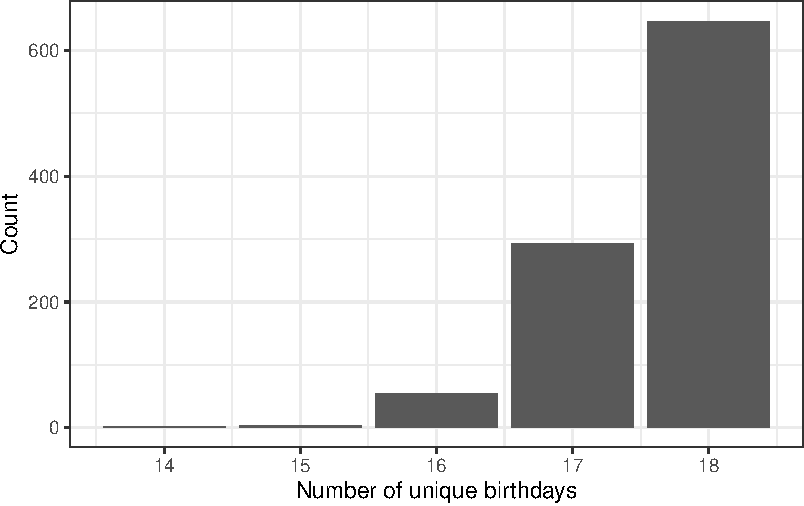
\includegraphics{Probability-Case-Study_files/figure-pdf/fig-bar71-1.pdf}

}

\caption{\label{fig-bar71}Bar chart of the number of unique birthdays in
the sample.}

\end{figure}%

\begin{quote}
\textbf{Exercise}:\\
What does it mean if the length of unique birthdays is 16, in terms of
matches?\footnote{It is possible that 3 people all have the same
  birthday or two sets of 2 people have the same birthday but different
  from the other pair.}
\end{quote}

\subsection{The mathematical approach}\label{the-mathematical-approach}

To solve this problem mathematically, we will work through the logic one
step at a time. One of the key ideas that we will see many times is the
idea of the \textbf{multiplication} rule. This idea is the foundation
for \textbf{permutations} and \textbf{combinations}, which are counting
methods frequently used in probability calculations.

The first step that we take is to understand the idea of two or more
people having the same birthday. With 18 people, there are a great deal
of possibilities for two or more people to have the same birthday. We
could have exactly two people with the same birthday. We could have 18
people with the same birthday. We could have three people with the same
birthday and another two people with the same birthday but different
from the other three. Accounting for all these possibilities is too
large a counting process. Instead, we will take the approach of finding
the probability of no one having a matching birthday. Then the
probability of at least two people having a matching birthday is one
minus the probability that no one has a matching birthday. This is known
as a \textbf{complementary} probability. A simpler example is to think
about rolling a single die. The probability of rolling a six is
equivalent to one minus the probability of not rolling a six (rolling
any number other than six).

We first need to think about all the different ways we could get 18
birthdays. This is going to be our denominator in the probability
calculation. The first person could have 365 different days for their
birthday. The second person could also have 365 different birthdays. The
same is true for all 18 people. This is an example of the
\emph{multiplication rule}. For 18 people, there are \(365^{18}\)
possible sets of birthdays.\footnote{\(365^{18} = 1.322\times 10^{46}\)}
Again, this will be our denominator in calculating the probability.

Because we're using the complement, the numerator is the number of ways
that 18 people can have birthdays with no matches.

\begin{quote}
Exercise:\\
What is the number of ways for 18 people to have no birthday matches?
\end{quote}

The first person can have a birthday on any day of the year, so there
are 365 possibilities. Because we don't want a match, the second person
only has 364 possibilities for a birthday. The third person can't match
either of the first two, so there are only 363 possibilities for that
birthday. Thus, there are
\(365 \times 364 \times 363 ... \times 349 \times 348\) ways for 18
people to have no birthday matches.

This looks like a truncated factorial. Remember a factorial, written as
\(n!\) with an explanation point, is the product of successive positive
integers. For example, \(3!\) is \(3 \times 2 \times 1\) or 6. In our
birthday example, we could write the multiplication for the numerator as
\[365\times 364\times ...\times 348 = \frac{365!}{(365-18)!}\] As we
will learn, the multiplication rule for the numerator is known as a
\textbf{permutation}.\footnote{This could be more generally written as
  \(\frac{365!}{(365 - n)!}\) for a group of \(n\) people.}

We are ready to put it all together. For 18 people, the probability of
two or more people with the same birthday is one minus the probability
that no one has the same birthday, which is

\[1 - \frac{\frac{365!}{(365-18)!}}{365^{18}}\] or

\[1 - \frac{\frac{365!}{347!}}{365^{18}}\]

In \texttt{R}, there is a \texttt{factorial()} function but factorials
get large fast and will \textbf{overflow} the memory. Try
\texttt{factorial(365)} in \texttt{R} to see what happens.

\begin{Shaded}
\begin{Highlighting}[]
\FunctionTok{factorial}\NormalTok{(}\DecValTok{365}\NormalTok{)}
\end{Highlighting}
\end{Shaded}

\begin{verbatim}
[1] Inf
\end{verbatim}

It is returning \emph{infinity} because the number is too large for the
buffer. As is often the case when using a computational method, we must
be clever about our approach. Instead of using factorials, we can make
use of \texttt{R} and its ability to work on vectors. If we provide
\texttt{R} with a vector of values, the \texttt{prod()} function will
calculate the product of all the elements.

\begin{Shaded}
\begin{Highlighting}[]
\DecValTok{365}\SpecialCharTok{*}\DecValTok{364}
\end{Highlighting}
\end{Shaded}

\begin{verbatim}
[1] 132860
\end{verbatim}

\begin{Shaded}
\begin{Highlighting}[]
\FunctionTok{prod}\NormalTok{(}\DecValTok{365}\SpecialCharTok{:}\DecValTok{364}\NormalTok{)}
\end{Highlighting}
\end{Shaded}

\begin{verbatim}
[1] 132860
\end{verbatim}

Now, we calculate the probability of at least two people in a room of 18
having the same birthday.

\begin{Shaded}
\begin{Highlighting}[]
\DecValTok{1}\SpecialCharTok{{-}} \FunctionTok{prod}\NormalTok{(}\DecValTok{365}\SpecialCharTok{:}\DecValTok{348}\NormalTok{) }\SpecialCharTok{/}\NormalTok{ (}\DecValTok{365}\SpecialCharTok{\^{}}\DecValTok{18}\NormalTok{)}
\end{Highlighting}
\end{Shaded}

\begin{verbatim}
[1] 0.3469114
\end{verbatim}

This is close to the probability we found with simulation.

\subsection{General solution}\label{general-solution}

We now have the mathematics to understand the problem. We can easily
generalize this to any number of people. To do this, we have to write a
function in \texttt{R}. As with everything in \texttt{R}, we save a
function as an object. The general format for creating a function is

\begin{Shaded}
\begin{Highlighting}[]
\NormalTok{my\_function }\OtherTok{\textless{}{-}} \ControlFlowTok{function}\NormalTok{(parameters)\{}
\NormalTok{  code }\ControlFlowTok{for} \ControlFlowTok{function}
\NormalTok{\}}
\end{Highlighting}
\end{Shaded}

For this problem we will call the function \texttt{birthday\_prob()}.
The only parameter we need is the number of people in the room,
\texttt{n}. Let's write this function.

\begin{Shaded}
\begin{Highlighting}[]
\NormalTok{birthday\_prob }\OtherTok{\textless{}{-}} \ControlFlowTok{function}\NormalTok{(}\AttributeTok{n=}\DecValTok{20}\NormalTok{)\{}
  \DecValTok{1} \SpecialCharTok{{-}} \FunctionTok{prod}\NormalTok{(}\DecValTok{365}\SpecialCharTok{:}\NormalTok{(}\DecValTok{365} \SpecialCharTok{{-}}\NormalTok{ (n }\SpecialCharTok{{-}} \DecValTok{1}\NormalTok{))) }\SpecialCharTok{/}\NormalTok{ (}\DecValTok{365}\SpecialCharTok{\^{}}\NormalTok{n)}
\NormalTok{\}}
\end{Highlighting}
\end{Shaded}

Notice we assigned the function to the name \texttt{birthday\_prob}, we
told \texttt{R} to expect one argument to the function, which we are
calling \texttt{n}, and then we provide \texttt{R} with the code to find
the probability. We set a default value for \texttt{n} in case one is
not provided to prevent an error when the function is run. We will learn
more about writing functions throughout this book and in the follow-on
USAFA course, Math 378: Applied Statistical Modeling.

Let's test the code with a known answer.

\begin{Shaded}
\begin{Highlighting}[]
\FunctionTok{birthday\_prob}\NormalTok{(}\DecValTok{18}\NormalTok{)}
\end{Highlighting}
\end{Shaded}

\begin{verbatim}
[1] 0.3469114
\end{verbatim}

Now we can determine the probability for any size room. You may have
heard that it only takes about 23 people in a room to have a 50\%
probability of at least two people matching birthdays.

\begin{Shaded}
\begin{Highlighting}[]
\FunctionTok{birthday\_prob}\NormalTok{(}\DecValTok{23}\NormalTok{)}
\end{Highlighting}
\end{Shaded}

\begin{verbatim}
[1] 0.5072972
\end{verbatim}

Let's create a plot of the probability versus the number of people in
the room. To do this, we need to apply the function to a vector of
values. The function \texttt{sapply()} will work or we can also use
\texttt{Vectorize()} to alter our existing function. We choose the
latter option.

First notice what happens if we input a vector into our function.

\begin{Shaded}
\begin{Highlighting}[]
\FunctionTok{birthday\_prob}\NormalTok{(}\DecValTok{1}\SpecialCharTok{:}\DecValTok{20}\NormalTok{)}
\end{Highlighting}
\end{Shaded}

\begin{verbatim}
Warning in 365:(365 - (n - 1)): numerical expression has 20 elements: only the
first used
\end{verbatim}

\begin{verbatim}
 [1] 0.0000000 0.9972603 0.9999925 1.0000000 1.0000000 1.0000000 1.0000000
 [8] 1.0000000 1.0000000 1.0000000 1.0000000 1.0000000 1.0000000 1.0000000
[15] 1.0000000 1.0000000 1.0000000 1.0000000 1.0000000 1.0000000
\end{verbatim}

It only uses the first value. There are several ways to solve this
problem. We can use the \texttt{map()} function in the \textbf{purrr}
package. This idea of mapping a function to a vector is important in
data science. It is used in scenarios where there is a lot of data. In
this case, the idea of map-reduce is used to make the analysis amenable
to parallel computing.

\begin{Shaded}
\begin{Highlighting}[]
\FunctionTok{map\_dbl}\NormalTok{(}\DecValTok{1}\SpecialCharTok{:}\DecValTok{20}\NormalTok{, birthday\_prob)}
\end{Highlighting}
\end{Shaded}

\begin{verbatim}
 [1] 0.000000000 0.002739726 0.008204166 0.016355912 0.027135574 0.040462484
 [7] 0.056235703 0.074335292 0.094623834 0.116948178 0.141141378 0.167024789
[13] 0.194410275 0.223102512 0.252901320 0.283604005 0.315007665 0.346911418
[19] 0.379118526 0.411438384
\end{verbatim}

We could also just vectorize the function.

\begin{Shaded}
\begin{Highlighting}[]
\NormalTok{birthday\_prob }\OtherTok{\textless{}{-}} \FunctionTok{Vectorize}\NormalTok{(birthday\_prob)}
\end{Highlighting}
\end{Shaded}

Now notice what happens.

\begin{Shaded}
\begin{Highlighting}[]
\FunctionTok{birthday\_prob}\NormalTok{(}\DecValTok{1}\SpecialCharTok{:}\DecValTok{20}\NormalTok{)}
\end{Highlighting}
\end{Shaded}

\begin{verbatim}
 [1] 0.000000000 0.002739726 0.008204166 0.016355912 0.027135574 0.040462484
 [7] 0.056235703 0.074335292 0.094623834 0.116948178 0.141141378 0.167024789
[13] 0.194410275 0.223102512 0.252901320 0.283604005 0.315007665 0.346911418
[19] 0.379118526 0.411438384
\end{verbatim}

We now have what we want, so let's create our line plot,
Figure~\ref{fig-line71}.

\begin{Shaded}
\begin{Highlighting}[]
\FunctionTok{gf\_line}\NormalTok{(}\FunctionTok{birthday\_prob}\NormalTok{(}\DecValTok{1}\SpecialCharTok{:}\DecValTok{100}\NormalTok{) }\SpecialCharTok{\textasciitilde{}} \FunctionTok{seq}\NormalTok{(}\DecValTok{1}\NormalTok{, }\DecValTok{100}\NormalTok{),}
        \AttributeTok{xlab =} \StringTok{"Number of People"}\NormalTok{,}
        \AttributeTok{ylab =} \StringTok{"Probability of Match"}\NormalTok{,}
        \AttributeTok{title =} \StringTok{"Probability of at least two people with matching birthdays by room size"}\NormalTok{) }\SpecialCharTok{\%\textgreater{}\%}
  \FunctionTok{gf\_theme}\NormalTok{(}\FunctionTok{theme\_bw}\NormalTok{())}
\end{Highlighting}
\end{Shaded}

\begin{figure}[H]

\centering{

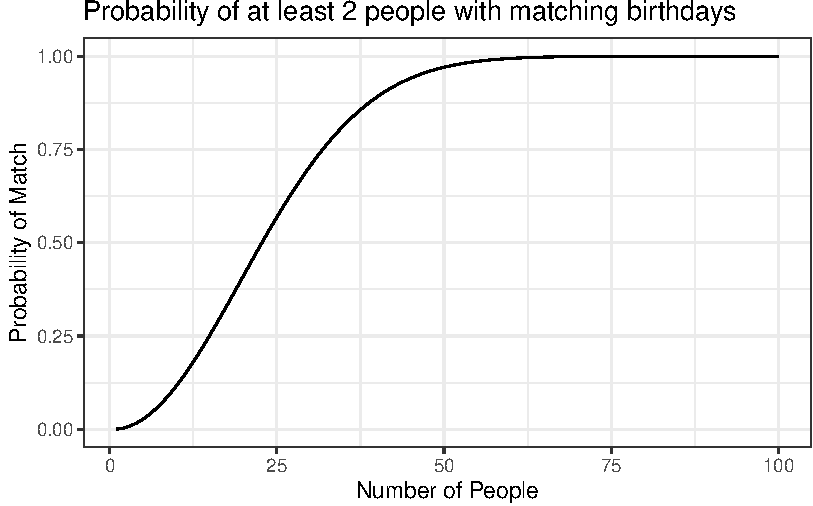
\includegraphics{Probability-Case-Study_files/figure-pdf/fig-line71-1.pdf}

}

\caption{\label{fig-line71}The probability of at least 2 people having
matching birthdays.}

\end{figure}%

Is this what you expected the curve to look like? We, the authors, did
not expect this. It has a sigmoidal shape with a large increase in the
middle range and flattening in the tails.

\subsection{Data science approach}\label{data-science-approach}

The final approach we will take is one based on data, a data science
approach. The \textbf{mosaicData} package includes a data set called
\texttt{Births} that contains the number of births in the US from 1969
to 1988. This data will allow us to estimate the number of births on any
day of the year. This allows us to eliminate the reliance on the
assumption that each day is equally likely. Let's first
\texttt{inspect()} the data object.

\begin{Shaded}
\begin{Highlighting}[]
\FunctionTok{inspect}\NormalTok{(Births)}
\end{Highlighting}
\end{Shaded}

\begin{verbatim}

categorical variables:  
  name   class levels    n missing
1 wday ordered      7 7305       0
                                   distribution
1 Wed (14.3%), Thu (14.3%), Fri (14.3%) ...    

Date variables:  
  name class      first       last min_diff max_diff    n missing
1 date  Date 1969-01-01 1988-12-31   1 days   1 days 7305       0

quantitative variables:  
          name   class  min   Q1 median    Q3   max        mean          sd
1       births integer 6675 8792   9622 10510 12851 9648.940178 1127.315229
2         year integer 1969 1974   1979  1984  1988 1978.501027    5.766735
3        month integer    1    4      7    10    12    6.522930    3.448939
4  day_of_year integer    1   93    184   275   366  183.753593  105.621885
5 day_of_month integer    1    8     16    23    31   15.729637    8.800694
6  day_of_week integer    1    2      4     6     7    4.000274    1.999795
     n missing
1 7305       0
2 7305       0
3 7305       0
4 7305       0
5 7305       0
6 7305       0
\end{verbatim}

Notice there are leap years present in this data. It could be argued
that we could randomly pick one year and use it. Let's see what happens
if we just used 1969, a non-leap year. Figure~\ref{fig-scat71} is a
scatter plot of the number of births in 1969 for each day of the year.

\begin{Shaded}
\begin{Highlighting}[]
\NormalTok{Births }\SpecialCharTok{\%\textgreater{}\%}
  \FunctionTok{filter}\NormalTok{(year }\SpecialCharTok{==} \DecValTok{1969}\NormalTok{) }\SpecialCharTok{\%\textgreater{}\%}
  \FunctionTok{gf\_point}\NormalTok{(births }\SpecialCharTok{\textasciitilde{}}\NormalTok{ day\_of\_year) }\SpecialCharTok{\%\textgreater{}\%}
  \FunctionTok{gf\_theme}\NormalTok{(}\FunctionTok{theme\_bw}\NormalTok{()) }\SpecialCharTok{\%\textgreater{}\%}
  \FunctionTok{gf\_labs}\NormalTok{(}\AttributeTok{x =} \StringTok{"Day of the Year"}\NormalTok{, }\AttributeTok{y =} \StringTok{"Number of Births"}\NormalTok{)}
\end{Highlighting}
\end{Shaded}

\begin{figure}[H]

\centering{

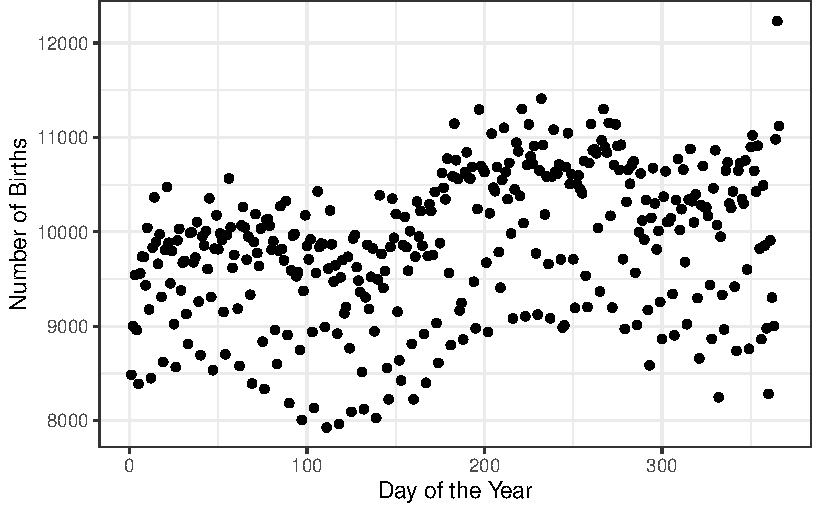
\includegraphics{Probability-Case-Study_files/figure-pdf/fig-scat71-1.pdf}

}

\caption{\label{fig-scat71}The number of births for each day of the year
in 1969.}

\end{figure}%

\begin{quote}
\textbf{Exercise}:\\
What patterns do you see in Figure~\ref{fig-scat71}? What might explain
them?\footnote{This could be due to doctors tending not to schedule
  inductions or C-sections on weekends. Fun fact: while more than 30\%
  of all births were C-sections in 2023, only around 5\% of births were
  C-sections in 1969.}
\end{quote}

There are definitely bands appearing in the data which could be the day
of the week; there are fewer birthdays on the weekend. There is also
seasonality with more birthdays in the summer and fall. There is also
probably an impact from holidays.

Quickly, let's look at the impact of day of the week by using color for
day of the week. Figure~\ref{fig-scat72} makes it clear that the
weekends have fewer births as compared to the work week.

\begin{Shaded}
\begin{Highlighting}[]
\NormalTok{Births }\SpecialCharTok{\%\textgreater{}\%}
  \FunctionTok{filter}\NormalTok{(year }\SpecialCharTok{==} \DecValTok{1969}\NormalTok{) }\SpecialCharTok{\%\textgreater{}\%}
  \FunctionTok{gf\_point}\NormalTok{(births }\SpecialCharTok{\textasciitilde{}}\NormalTok{ day\_of\_year, }\AttributeTok{color =} \SpecialCharTok{\textasciitilde{}}\FunctionTok{factor}\NormalTok{(day\_of\_week)) }\SpecialCharTok{\%\textgreater{}\%}
  \FunctionTok{gf\_labs}\NormalTok{(}\AttributeTok{x =} \StringTok{"Day of the Year"}\NormalTok{, }\AttributeTok{col =} \StringTok{"Day of Week"}\NormalTok{) }\SpecialCharTok{\%\textgreater{}\%}
  \FunctionTok{gf\_theme}\NormalTok{(}\FunctionTok{theme\_bw}\NormalTok{())}
\end{Highlighting}
\end{Shaded}

\begin{figure}[H]

\centering{

\includegraphics{Probability-Case-Study_files/figure-pdf/fig-scat72-1.pdf}

}

\caption{\label{fig-scat72}The number of births for each day of the year
in 1969 broken down by day of the week.}

\end{figure}%

By only using one year, this data might give poor results because
holidays will fall on certain days of the week and the weekends will
also be impacted. Note that we also still have the problem of leap
years.

\begin{Shaded}
\begin{Highlighting}[]
\NormalTok{Births }\SpecialCharTok{\%\textgreater{}\%}
  \FunctionTok{group\_by}\NormalTok{(year) }\SpecialCharTok{\%\textgreater{}\%}
  \FunctionTok{summarise}\NormalTok{(}\AttributeTok{n =} \FunctionTok{n}\NormalTok{())}
\end{Highlighting}
\end{Shaded}

\begin{verbatim}
# A tibble: 20 x 2
    year     n
   <int> <int>
 1  1969   365
 2  1970   365
 3  1971   365
 4  1972   366
 5  1973   365
 6  1974   365
 7  1975   365
 8  1976   366
 9  1977   365
10  1978   365
11  1979   365
12  1980   366
13  1981   365
14  1982   365
15  1983   365
16  1984   366
17  1985   365
18  1986   365
19  1987   365
20  1988   366
\end{verbatim}

The years 1972, 1976, 1980, 1984, and 1988 are all leap years. At this
point, to make the analysis easier, we will drop those years.

\begin{Shaded}
\begin{Highlighting}[]
\NormalTok{Births }\SpecialCharTok{\%\textgreater{}\%}
  \FunctionTok{filter}\NormalTok{(}\SpecialCharTok{!}\NormalTok{(year }\SpecialCharTok{\%in\%} \FunctionTok{c}\NormalTok{(}\DecValTok{1972}\NormalTok{, }\DecValTok{1976}\NormalTok{, }\DecValTok{1980}\NormalTok{, }\DecValTok{1984}\NormalTok{, }\DecValTok{1988}\NormalTok{))) }\SpecialCharTok{\%\textgreater{}\%}
  \FunctionTok{group\_by}\NormalTok{(year) }\SpecialCharTok{\%\textgreater{}\%}
  \FunctionTok{summarise}\NormalTok{(}\AttributeTok{n =} \FunctionTok{n}\NormalTok{())}
\end{Highlighting}
\end{Shaded}

\begin{verbatim}
# A tibble: 15 x 2
    year     n
   <int> <int>
 1  1969   365
 2  1970   365
 3  1971   365
 4  1973   365
 5  1974   365
 6  1975   365
 7  1977   365
 8  1978   365
 9  1979   365
10  1981   365
11  1982   365
12  1983   365
13  1985   365
14  1986   365
15  1987   365
\end{verbatim}

Notice that we used the \texttt{\%in\%} operator inside the
\texttt{filter()} function. This is a \textbf{logical} argument checking
whether \texttt{year} is one of the specified values. The \texttt{!} at
the front negates this, in a sense requiring \texttt{year} to not be one
of those values.

We are almost ready to simulate. We need to get the count of
\texttt{births} on each day of the year for the non-leap years.

\begin{Shaded}
\begin{Highlighting}[]
\NormalTok{birth\_data }\OtherTok{\textless{}{-}}\NormalTok{ Births }\SpecialCharTok{\%\textgreater{}\%}
  \FunctionTok{filter}\NormalTok{(}\SpecialCharTok{!}\NormalTok{(year }\SpecialCharTok{\%in\%} \FunctionTok{c}\NormalTok{(}\DecValTok{1972}\NormalTok{, }\DecValTok{1976}\NormalTok{, }\DecValTok{1980}\NormalTok{, }\DecValTok{1984}\NormalTok{, }\DecValTok{1988}\NormalTok{))) }\SpecialCharTok{\%\textgreater{}\%}
  \FunctionTok{group\_by}\NormalTok{(day\_of\_year) }\SpecialCharTok{\%\textgreater{}\%}
  \FunctionTok{summarise}\NormalTok{(}\AttributeTok{n =} \FunctionTok{sum}\NormalTok{(births)) }
\end{Highlighting}
\end{Shaded}

\begin{Shaded}
\begin{Highlighting}[]
\FunctionTok{head}\NormalTok{(birth\_data)}
\end{Highlighting}
\end{Shaded}

\begin{verbatim}
# A tibble: 6 x 2
  day_of_year      n
        <int>  <int>
1           1 120635
2           2 129042
3           3 135901
4           4 136298
5           5 137319
6           6 140044
\end{verbatim}

Let's look at a plot of the number of births versus day of the year for
all the non-leap years in Figure~\ref{fig-scat73}.

\begin{Shaded}
\begin{Highlighting}[]
\NormalTok{birth\_data }\SpecialCharTok{\%\textgreater{}\%}
  \FunctionTok{gf\_point}\NormalTok{(n }\SpecialCharTok{\textasciitilde{}}\NormalTok{ day\_of\_year,}
          \AttributeTok{xlab =} \StringTok{"Day of the year"}\NormalTok{,}
          \AttributeTok{ylab =} \StringTok{"Number of births"}\NormalTok{) }\SpecialCharTok{\%\textgreater{}\%}
  \FunctionTok{gf\_theme}\NormalTok{(}\FunctionTok{theme\_bw}\NormalTok{())}
\end{Highlighting}
\end{Shaded}

\begin{figure}[H]

\centering{

\includegraphics{Probability-Case-Study_files/figure-pdf/fig-scat73-1.pdf}

}

\caption{\label{fig-scat73}Number of births by day of the year for all
years.}

\end{figure}%

This curve has the seasonal cycling we would expect. The smaller scale
cycling is unexpected. Maybe because we are dropping the leap years, we
are getting some days appearing in our time interval more frequently on
weekends. We leave it to you to investigate this phenomenon.

We use these counts as weights in a sampling process. Days with more
births will have a higher probability of being selected. Days such as
Christmas and Christmas Eve have a lower probability of being selected.
Let's save the weights in an object to use in the \texttt{sample()}
function.

\begin{Shaded}
\begin{Highlighting}[]
\NormalTok{birth\_data\_weights }\OtherTok{\textless{}{-}}\NormalTok{ birth\_data }\SpecialCharTok{\%\textgreater{}\%}
  \FunctionTok{select}\NormalTok{(n) }\SpecialCharTok{\%\textgreater{}\%}
  \FunctionTok{pull}\NormalTok{()}
\end{Highlighting}
\end{Shaded}

The \texttt{pull()} function pulls the vectors of values out of the data
frame format into a vector format which the \texttt{sample()} function
needs.

Now let's simulate the problem. We will use our code from before, but
add probability weights in the \texttt{prob} argument. The probability
of a match should change slightly, but not much because most of the days
have about the same probability or number of occurrences.

\begin{Shaded}
\begin{Highlighting}[]
\FunctionTok{set.seed}\NormalTok{(}\DecValTok{20}\NormalTok{)}
\NormalTok{(}\FunctionTok{do}\NormalTok{(}\DecValTok{1000}\NormalTok{)}\SpecialCharTok{*}\FunctionTok{length}\NormalTok{(}\FunctionTok{unique}\NormalTok{(}\FunctionTok{sample}\NormalTok{(days, }\AttributeTok{size =} \DecValTok{18}\NormalTok{, }\AttributeTok{replace =} \ConstantTok{TRUE}\NormalTok{, }\AttributeTok{prob =}\NormalTok{ birth\_data\_weights)))) }\SpecialCharTok{\%\textgreater{}\%}
  \FunctionTok{mutate}\NormalTok{(}\AttributeTok{match =} \FunctionTok{if\_else}\NormalTok{(length }\SpecialCharTok{==} \DecValTok{18}\NormalTok{, }\DecValTok{0}\NormalTok{, }\DecValTok{1}\NormalTok{)) }\SpecialCharTok{\%\textgreater{}\%}
  \FunctionTok{summarise}\NormalTok{(}\AttributeTok{prob =} \FunctionTok{mean}\NormalTok{(match))}
\end{Highlighting}
\end{Shaded}

\begin{verbatim}
   prob
1 0.352
\end{verbatim}

It would not be possible to solve this problem of varying frequency of
birthdays using mathematics, at least as far as we know.

This is fascinating stuff! Let's get to learning more about probability
models in the following chapters.

\chapter{Probability Rules}\label{sec-PROBRULES}

\section{Objectives}\label{objectives-8}

\begin{enumerate}
\def\labelenumi{\arabic{enumi})}
\item
  Differentiate between various statistical terminologies such as
  \emph{sample space, outcome, event, subset, intersection, union,
  complement, probability, mutually exclusive, exhaustive, independent,
  multiplication rule, permutation,} and \emph{combination}, and
  construct examples to demonstrate their proper use in context.
\item
  Apply basic probability properties and counting rules to calculate the
  probabilities of events in different scenarios. Interpret the
  calculated probabilities in context.
\item
  Explain and illustrate the basic axioms of probability.
\item
  Use \texttt{R} to perform calculations and simulations for determining
  the probabilities of events.
\end{enumerate}

\section{Probability vs Statistics}\label{probability-vs-statistics}

Remember this book is divided into four general blocks: data
collection/summary, probability models, inference and statistical
modeling/prediction. This second block on probability models is the
study of stochastic (random) processes and their properties.
Specifically, we will explore random experiments. As the name suggests,
a random experiment is an experiment whose outcome is not predictable
with exact certainty. In the statistical models we develop in the last
two blocks of this book, we will use other variables to explain the
variance of the outcome of interest. Any remaining variance is modeled
with probability models.

Even though an outcome is determined by chance, this does not mean that
we know nothing about the random experiment. Our favorite simple example
is that of a coin flip. If we flip a coin, the possible outcomes are
heads and tails. We don't know for sure what outcome will occur, but we
still know something about the experiment. If we assume the coin is
fair, we know that each outcome is equally likely. Also, we know that if
we flip the coin 100 times (independently), we are likely to see around
50 heads, and very unlikely to see 10 heads or fewer.

It is important to distinguish probability from inference and modeling.
In probability, we consider a known random experiment, including knowing
the parameters, and answer questions about what we expect to see from
this random experiment. In statistics (inference and modeling), we
consider data (the results of a mysterious random experiment) and infer
about the underlying process. For example, suppose we have a coin and we
are unsure whether this coin is fair or unfair (i.e., the parameter is
unknown). We might flip it 20 times and observe it land on heads 14
times. Inferential statistics will help us answer questions about the
underlying process (e.g., could this coin be unfair?).

\begin{figure}[H]

{\centering \includegraphics{figures/Prob_Stats.png}

}

\caption{A graphical representation of probability and statistics. In
probability, we describe what we expect to happen if we know about the
underlying process. In statistics, we don't know the underlying process,
and must infer based on representative samples.}

\end{figure}%

This block (10 chapters or so) is devoted to the study of random
experiments. First, we will explore simple experiments, counting rule
problems, and conditional probability. Next, we will introduce the
concept of a random variable and the properties of random variables.
Following this, we will cover common distributions of discrete and
continuous random variables. We will end the block on multivariate
probability (joint distributions and covariance).

\section{Basic probability terms}\label{basic-probability-terms}

We will start our work with some definitions and examples.

\subsection{Sample space}\label{sample-space}

Suppose we have a random experiment. The \emph{sample space} of this
experiment, \(S\), is the set of all possible results of that
experiment. For example, in the case of a coin flip, we could write
\(S=\{H,T\}\) because the sample space has two outcomes, heads and
tails. Each element of the sample space is considered an \emph{outcome}.
An \emph{event} is a set of outcomes, a subset of the sample space.

\begin{quote}
\emph{Example}:\\
Let \texttt{R} flip a coin for us and record the number of heads and
tails. We will have \texttt{R} flip the coin twice. What is the sample
space, what is an example of an outcome, and what is an example of an
event?
\end{quote}

We will load the \textbf{mosaic} package as it has a function
\texttt{rflip()} that will simulate flipping a coin.

\begin{Shaded}
\begin{Highlighting}[]
\FunctionTok{library}\NormalTok{(mosaic)}
\end{Highlighting}
\end{Shaded}

\begin{Shaded}
\begin{Highlighting}[]
\FunctionTok{set.seed}\NormalTok{(}\DecValTok{18}\NormalTok{)}
\FunctionTok{rflip}\NormalTok{(}\DecValTok{2}\NormalTok{)}
\end{Highlighting}
\end{Shaded}

\begin{verbatim}

Flipping 2 coins [ Prob(Heads) = 0.5 ] ...

H H

Number of Heads: 2 [Proportion Heads: 1]
\end{verbatim}

The sample space is \(S=\{HH, TH, HT, TT\}\), an example of an outcome
is \(HH\) which we see in the output from \texttt{R}, and an example of
an event is two tails, \({TT}\). Another example of an event is ``at
least one heads'', \(\{HH,TH, HT\}\). Also, notice that \(TH\) is
different from \(HT\) as an outcome; this is because those are different
outcomes from flipping a coin twice.

\begin{quote}
\emph{Example of Event}:\\
Suppose you arrive at a rental car counter and they show you a list of
available vehicles, and one is picked for you at random. The sample
space in this experiment is \[
S=\{\mbox{red sedan}, \mbox{blue sedan}, \mbox{red truck}, \mbox{grey truck}, \mbox{grey SUV}, \mbox{black SUV}, \mbox{blue SUV}\}.
\]

Each vehicle represents a possible outcome of the experiment.
\end{quote}

\subsection{Union and intersection}\label{union-and-intersection}

Suppose we have two events, \(A\) and \(B\).

\begin{enumerate}
\def\labelenumi{\arabic{enumi})}
\item
  \(A\) is considered a \emph{subset} of \(B\) if all of the outcomes of
  \(A\) are also contained in \(B\). This is denoted as \(A \subset B\).
\item
  The \emph{intersection} of \(A\) and \(B\) is all of the outcomes
  contained in both \(A\) and \(B\). This is denoted as \(A \cap B\).
\item
  The \emph{union} of \(A\) and \(B\) is all of the outcomes contained
  in either \(A\) or \(B\), or both. This is denoted as \(A \cup B\).
\item
  The \emph{complement} of \(A\) is all of the outcomes not contained in
  \(A\). This is denoted as \(A^C\) or \(A'\).
\end{enumerate}

Note: Here we are treating events as sets and the above definitions are
basic set operations.

It is sometimes helpful when reading probability notation to think of
Union as an \emph{or} and Intersection as an \emph{and}.

\begin{quote}
\emph{Example}:\\
Consider our rental car example above. Let \(A\) be the event that a
blue vehicle is selected, let \(B\) be the event that a black vehicle is
selected, and let \(C\) be the event that an SUV is selected.
\end{quote}

First, let's list all of the outcomes of each event.
\(A = \{\mbox{blue sedan},\mbox{blue SUV}\}\),
\(B=\{\mbox{black SUV}\}\), and
\(C= \{\mbox{grey SUV}, \mbox{black SUV}, \mbox{blue SUV}\}\).

Because all outcomes in \(B\) are contained in \(C\), we know that \(B\)
is a subset of \(C\). This can be written as \(B\subset C\). Also,
because \(A\) and \(B\) have no outcomes in common,
\(A \cap B = \emptyset\). Note that \(\emptyset = \{ \}\) is the empty
set and contains no elements.\footnote{We call events \(A\) and \(B\)
  \emph{mutually exclusive}. We'll define this term a little later in
  the chapter.} Further,
\(A \cup C = \{\mbox{blue sedan}, \mbox{grey SUV}, \mbox{black SUV}, \mbox{blue SUV}\}\).
The complement of \(C\) is
\(C'=\{\text{red sedan, red truck, grey truck}\}\).

\section{Probability}\label{probability}

\emph{Probability} is a number assigned to an event or outcome that
describes how likely it is to occur. A probability model assigns a
probability to each element of the sample space. What makes a
probability model is not just the values assigned to each element but
the idea that this model contains all the information about the outcomes
and there are no other explanatory variables involved.

A probability model can be thought of as a function that maps outcomes,
or events, to a real number in the interval \([0,1]\).

\subsection{Probability axioms}\label{probability-axioms}

There are some basic axioms of probability you should know, although
this list is not complete. Let \(S\) be the sample space of a random
experiment and let \(A\) be an event where \(A\subset S\).

\begin{enumerate}
\def\labelenumi{\arabic{enumi})}
\item
  \(\mbox{P}(A) \geq 0\).
\item
  \(\mbox{P}(S) = 1\).
\end{enumerate}

These two axioms essentially say that probability must be positive, and
the probability of all outcomes must sum to one.

\subsection{Probability properties}\label{probability-properties}

Let \(A\) and \(B\) be events in a random experiment. Most of the
probabilities below can be proven fairly easily.

\begin{enumerate}
\def\labelenumi{\arabic{enumi})}
\item
  \(\mbox{P}(\emptyset)=0\).
\item
  \(\mbox{P}(A')=1-\mbox{P}(A)\). We used this in the case study.
\item
  If \(A\subset B\), then \(\mbox{P}(A)\leq \mbox{P}(B)\).
\item
  \(\mbox{P}(A\cup B) = \mbox{P}(A)+\mbox{P}(B)-\mbox{P}(A\cap B)\).
  This property can be generalized to more than two events. The
  intersection is subtracted because outcomes in both events \(A\) and
  \(B\) get counted twice in the first sum.
\item
  Law of Total Probability: Let \(B_1, B_2,...,B_n\) be \textbf{mutually
  exclusive}, this means disjoint or no outcomes in common, and
  \textbf{exhaustive}, this means the union of all the events labeled
  with a \(B\) is the sample space. Then
\end{enumerate}

\[
\mbox{P}(A)=\mbox{P}(A\cap B_1)+\mbox{P}(A\cap B_2)+...+\mbox{P}(A\cap B_n)
\]

A specific application of this law appears in Bayes' Rule (more to
follow in Chapter~\ref{sec-CONDPROB}). It says that
\(\mbox{P}(A)=\mbox{P}(A \cap B)+\mbox{P}(A \cap B')\). Essentially, it
points out that \(A\) can be partitioned into two parts: 1) everything
in \(A\) and \(B\) and 2) everything in \(A\) and not in \(B\).

\begin{quote}
\emph{Example}:\\
Consider rolling a six sided die. Let event \(A\) be that a number less
than five is showing on the die. Let event \(B\) be that . Then,

\[\mbox{P}(A)=\mbox{P}(A \cap B) + \mbox{P}(A \cap B')\]

\[
\mbox{P}(< 5)=\mbox{P}(<5 \cap \text{Even})+\mbox{P}(<5 \cap \text{Odd})
\]
\end{quote}

\begin{enumerate}
\def\labelenumi{\arabic{enumi})}
\setcounter{enumi}{5}
\tightlist
\item
  DeMorgan's Laws: \[
  \mbox{P}((A \cup B)')=\mbox{P}(A' \cap B')
  \] \[
  \mbox{P}((A \cap B)')=\mbox{P}(A' \cup B')
  \]
\end{enumerate}

\begin{quote}
\textbf{Exercise:} \emph{\hfill\break
}Let \(A\), \(B\), and \(C\) be events such that \(P(A)=0.5\),
\(P(B)=0.3\), and \(P(C)=0.4\). Also, we know that \(P(A\cap B)=0.2\),
\(P(B\cap C)=0.12\), \(P(A\cap C)=0.1\), and \(P(A\cap B\cap C)=0.05\).
Find the following:

\begin{itemize}
\item
  \(P(A\cup B)\)
\item
  \(P(A\cup B\cup C)\)
\item
  \(P(B'\cap C')\)
\item
  \(P(A\cup (B\cap C))\)
\item
  \(P((A\cup B\cup C)\cap (A\cap B\cap C)')\)
\end{itemize}
\end{quote}

It can be a good idea to draw a picture to work through exercises like
these. Figure~\ref{fig-prob-venn} is an illustration of the above
probability problem. Letters A, B, and C denote the corresponding
events, represented by the entire circle in which they reside. The
letter S represents the entire sample space. The numbers in the diagram
represent the probability of each exclusive event. For example, the
value 0.25 represents the probability of only event A (and no other
events). Can you figure out where the other probability values come
from?\footnote{The easiest way to create this illustration is to start
  from the middle intersection piece. \(P(A\cap B\cap C)=0.05\),
  represented by the 0.05 at the center of the diagram.
  \(P(A\cap B)=0.2\), which leaves 0.15 for the rest of the \(A\cap B\)
  piece of the diagram. Because \(P(A\cap C)=0.1\), the remaining piece
  of \(A\cap C\) not yet accounted for is 0.05. Then the remaining piece
  of \(A\) is 0.25. Thus, \(P(A)\) can be found by summing all the
  pieces in the \(A\) circle, which adds up to 0.5. Make sure you can
  track how the rest of the diagram is appropriately labeled.}

\begin{figure}

\centering{

\includegraphics{figures/prob_venn_diag.PNG}

}

\caption{\label{fig-prob-venn}Probability illustration.}

\end{figure}%

\subsection{Equally likely scenarios}\label{equally-likely-scenarios}

In some random experiments, outcomes can be defined such that each
individual outcome is equally likely. In this case, probability becomes
a counting problem. Let \(A\) be an event in an experiment where each
outcome is equally likely. \[
\mbox{P}(A)=\frac{\mbox{Number of outcomes in A}}{\mbox{Number of outcomes in S}}
\]

\begin{quote}
\emph{Example}:\\
Suppose a family has three children, with each child being either male
(M) or female (F). Assume that the likelihood of males and females are
equal and \textbf{independent}. This is the idea that the probability of
the sex of the second child does not change based on the sex of the
first child. The sample space can be written as: \[
S=\{\mbox{MMM},\mbox{MMF},\mbox{MFM},\mbox{FMM},\mbox{MFF},\mbox{FMF},\mbox{FFM},\mbox{FFF}\}
\] What is the probability that the family has exactly 2 female
children?
\end{quote}

This only happens in three ways: MFF, FMF, and FFM. Thus, the
probability of exactly 2 females is 3/8 or 0.375.

\subsection{\texorpdfstring{Simulation with \texttt{R} (Equally likely
scenarios)}{Simulation with R (Equally likely scenarios)}}\label{simulation-with-r-equally-likely-scenarios}

The previous example above is an example of an ``Equally Likely''
scenario, where the sample space of a random experiment contains a list
of outcomes that are equally likely. In these cases, we can sometimes
use \texttt{R} to list out the possible outcomes and count them to
determine probability. We can also use \texttt{R} to simulate the
scenario.

\begin{quote}
\emph{Example}:\\
Use \texttt{R} to simulate the family of three children where each child
has the same probability of being male or female.
\end{quote}

Instead of writing our own function, we can use \texttt{rflip()} in the
\textbf{mosaic} package. We will let \(H\) stand for female.

First simulate one family.

\begin{Shaded}
\begin{Highlighting}[]
\FunctionTok{set.seed}\NormalTok{(}\DecValTok{73}\NormalTok{)}
\FunctionTok{rflip}\NormalTok{(}\DecValTok{3}\NormalTok{)}
\end{Highlighting}
\end{Shaded}

\begin{verbatim}

Flipping 3 coins [ Prob(Heads) = 0.5 ] ...

T T H

Number of Heads: 1 [Proportion Heads: 0.333333333333333]
\end{verbatim}

In this case, we got 1 female. Next, we will use the \texttt{do()}
function to repeat this simulation.

\begin{Shaded}
\begin{Highlighting}[]
\NormalTok{results }\OtherTok{\textless{}{-}} \FunctionTok{do}\NormalTok{(}\DecValTok{10000}\NormalTok{)}\SpecialCharTok{*}\FunctionTok{rflip}\NormalTok{(}\DecValTok{3}\NormalTok{)}
\FunctionTok{head}\NormalTok{(results)}
\end{Highlighting}
\end{Shaded}

\begin{verbatim}
  n heads tails      prop
1 3     1     2 0.3333333
2 3     3     0 1.0000000
3 3     3     0 1.0000000
4 3     3     0 1.0000000
5 3     1     2 0.3333333
6 3     1     2 0.3333333
\end{verbatim}

Next, we can visualize the distribution of the number of females, heads,
in Figure @ref(fig:bar81-fig).

\begin{Shaded}
\begin{Highlighting}[]
\NormalTok{results }\SpecialCharTok{\%\textgreater{}\%}
  \FunctionTok{gf\_bar}\NormalTok{(}\SpecialCharTok{\textasciitilde{}}\NormalTok{heads) }\SpecialCharTok{\%\textgreater{}\%}
  \FunctionTok{gf\_theme}\NormalTok{(}\FunctionTok{theme\_bw}\NormalTok{()) }\SpecialCharTok{\%\textgreater{}\%}
  \FunctionTok{gf\_labs}\NormalTok{(}\AttributeTok{x =} \StringTok{"Number of females"}\NormalTok{, }\AttributeTok{y =} \StringTok{"Count"}\NormalTok{)}
\end{Highlighting}
\end{Shaded}

\begin{figure}[H]

{\centering \includegraphics{Probability-Rules_files/figure-pdf/bar81-fig-1.pdf}

}

\caption{Number of females in a family of size 3.}

\end{figure}%

Finally, we can estimate the probability of exactly 2 females. We need
the \textbf{tidyverse} library.

\begin{Shaded}
\begin{Highlighting}[]
\FunctionTok{library}\NormalTok{(tidyverse)}
\end{Highlighting}
\end{Shaded}

\begin{Shaded}
\begin{Highlighting}[]
\NormalTok{results }\SpecialCharTok{\%\textgreater{}\%}
  \FunctionTok{filter}\NormalTok{(heads }\SpecialCharTok{==} \DecValTok{2}\NormalTok{) }\SpecialCharTok{\%\textgreater{}\%}
  \FunctionTok{summarize}\NormalTok{(}\AttributeTok{prob =} \FunctionTok{n}\NormalTok{()}\SpecialCharTok{/}\DecValTok{10000}\NormalTok{)}
\end{Highlighting}
\end{Shaded}

\begin{verbatim}
    prob
1 0.3782
\end{verbatim}

Or we can use slightly different code.

\begin{Shaded}
\begin{Highlighting}[]
\NormalTok{results }\SpecialCharTok{\%\textgreater{}\%}
  \FunctionTok{count}\NormalTok{(heads) }\SpecialCharTok{\%\textgreater{}\%}
  \FunctionTok{mutate}\NormalTok{(}\AttributeTok{prop =}\NormalTok{ n}\SpecialCharTok{/}\FunctionTok{sum}\NormalTok{(n))}
\end{Highlighting}
\end{Shaded}

\begin{verbatim}
  heads    n   prop
1     0 1241 0.1241
2     1 3786 0.3786
3     2 3782 0.3782
4     3 1191 0.1191
\end{verbatim}

This is not a bad estimate of the exact probability, 0.375.

Let's now use an example of cards to simulate some probabilities and
learn more about counting. The file \texttt{Cards.csv} contains the data
for cards from a standard 52-card deck. There are four suits and two
colors: spades and clubs are black, hearts and diamonds are red. Within
each suit, there are 13 card values or ranks. These include ace, king,
queen, jack, and numbers ranging from ten down to two. Let's read in the
data and summarize.

\begin{Shaded}
\begin{Highlighting}[]
\NormalTok{Cards }\OtherTok{\textless{}{-}} \FunctionTok{read\_csv}\NormalTok{(}\StringTok{"data/Cards.csv"}\NormalTok{)}
\FunctionTok{inspect}\NormalTok{(Cards)}
\end{Highlighting}
\end{Shaded}

\begin{verbatim}

categorical variables:  
  name     class levels  n missing
1 rank character     13 52       0
2 suit character      4 52       0
                                   distribution
1 10 (7.7%), 2 (7.7%), 3 (7.7%) ...            
2 Club (25%), Diamond (25%) ...                

quantitative variables:  
   name   class        min         Q1     median         Q3        max
1 probs numeric 0.01923077 0.01923077 0.01923077 0.01923077 0.01923077
        mean sd  n missing
1 0.01923077  0 52       0
\end{verbatim}

\begin{Shaded}
\begin{Highlighting}[]
\FunctionTok{head}\NormalTok{(Cards)}
\end{Highlighting}
\end{Shaded}

\begin{verbatim}
# A tibble: 6 x 3
  rank  suit   probs
  <chr> <chr>  <dbl>
1 2     Club  0.0192
2 3     Club  0.0192
3 4     Club  0.0192
4 5     Club  0.0192
5 6     Club  0.0192
6 7     Club  0.0192
\end{verbatim}

We can see 4 suits, and 13 ranks, the value on the face of the card.

\begin{quote}
\emph{Example}:\\
Suppose we draw one card out of a standard deck. Let \(A\) be the event
that we draw a Club. Let \(B\) be the event that we draw a 10 or a face
card (Jack, Queen, King or Ace). We can use \texttt{R} to define these
events and find probabilities.
\end{quote}

Let's find all the Clubs.

\begin{Shaded}
\begin{Highlighting}[]
\NormalTok{Cards }\SpecialCharTok{\%\textgreater{}\%}
  \FunctionTok{filter}\NormalTok{(suit }\SpecialCharTok{==} \StringTok{"Club"}\NormalTok{) }\SpecialCharTok{\%\textgreater{}\%}
  \FunctionTok{select}\NormalTok{(rank, suit)}
\end{Highlighting}
\end{Shaded}

\begin{verbatim}
# A tibble: 13 x 2
   rank  suit 
   <chr> <chr>
 1 2     Club 
 2 3     Club 
 3 4     Club 
 4 5     Club 
 5 6     Club 
 6 7     Club 
 7 8     Club 
 8 9     Club 
 9 10    Club 
10 J     Club 
11 Q     Club 
12 K     Club 
13 A     Club 
\end{verbatim}

So just by counting, we find the probability of drawing a Club is
\(\frac{13}{52}\) or 0.25. We can also do this with simulation. This may
be overkill for this example, but it gets the idea of simulation across.

Remember, ask yourself what we want \texttt{R} to do and what \texttt{R}
needs to do this. Below we sample one card from ``the deck'' (i.e., the
data set) 10,000 times.

\begin{Shaded}
\begin{Highlighting}[]
\FunctionTok{set.seed}\NormalTok{(}\DecValTok{573}\NormalTok{)}
\NormalTok{results }\OtherTok{\textless{}{-}} \FunctionTok{do}\NormalTok{(}\DecValTok{10000}\NormalTok{)}\SpecialCharTok{*}\FunctionTok{sample}\NormalTok{(Cards, }\DecValTok{1}\NormalTok{)}
\FunctionTok{head}\NormalTok{(results)}
\end{Highlighting}
\end{Shaded}

\begin{verbatim}
# A tibble: 6 x 6
  rank  suit     probs orig.id  .row .index
  <chr> <chr>    <dbl> <chr>   <int>  <dbl>
1 2     Diamond 0.0192 14          1      1
2 7     Spade   0.0192 45          1      2
3 6     Spade   0.0192 44          1      3
4 3     Heart   0.0192 28          1      4
5 5     Diamond 0.0192 17          1      5
6 10    Spade   0.0192 48          1      6
\end{verbatim}

\begin{Shaded}
\begin{Highlighting}[]
\NormalTok{results }\SpecialCharTok{\%\textgreater{}\%}
  \FunctionTok{filter}\NormalTok{(suit }\SpecialCharTok{==} \StringTok{"Club"}\NormalTok{) }\SpecialCharTok{\%\textgreater{}\%}
  \FunctionTok{summarize}\NormalTok{(}\AttributeTok{prob =} \FunctionTok{n}\NormalTok{()}\SpecialCharTok{/}\DecValTok{10000}\NormalTok{)}
\end{Highlighting}
\end{Shaded}

\begin{verbatim}
# A tibble: 1 x 1
   prob
  <dbl>
1 0.240
\end{verbatim}

\begin{Shaded}
\begin{Highlighting}[]
\NormalTok{results }\SpecialCharTok{\%\textgreater{}\%}
  \FunctionTok{count}\NormalTok{(suit) }\SpecialCharTok{\%\textgreater{}\%}
  \FunctionTok{mutate}\NormalTok{(}\AttributeTok{prob =}\NormalTok{ n}\SpecialCharTok{/}\FunctionTok{sum}\NormalTok{(n))}
\end{Highlighting}
\end{Shaded}

\begin{verbatim}
# A tibble: 4 x 3
  suit        n  prob
  <chr>   <int> <dbl>
1 Club     2405 0.240
2 Diamond  2594 0.259
3 Heart    2529 0.253
4 Spade    2472 0.247
\end{verbatim}

In 10,000 samples, each suit occurs around 25\% of the time, just as
we'd expect.

Now let's count the number of outcomes in \(B\).

\begin{Shaded}
\begin{Highlighting}[]
\NormalTok{Cards }\SpecialCharTok{\%\textgreater{}\%}
  \FunctionTok{filter}\NormalTok{(rank }\SpecialCharTok{\%in\%} \FunctionTok{c}\NormalTok{(}\DecValTok{10}\NormalTok{, }\StringTok{"J"}\NormalTok{, }\StringTok{"Q"}\NormalTok{, }\StringTok{"K"}\NormalTok{, }\StringTok{"A"}\NormalTok{)) }\SpecialCharTok{\%\textgreater{}\%}
  \FunctionTok{select}\NormalTok{(rank,suit)}
\end{Highlighting}
\end{Shaded}

\begin{verbatim}
# A tibble: 20 x 2
   rank  suit   
   <chr> <chr>  
 1 10    Club   
 2 J     Club   
 3 Q     Club   
 4 K     Club   
 5 A     Club   
 6 10    Diamond
 7 J     Diamond
 8 Q     Diamond
 9 K     Diamond
10 A     Diamond
11 10    Heart  
12 J     Heart  
13 Q     Heart  
14 K     Heart  
15 A     Heart  
16 10    Spade  
17 J     Spade  
18 Q     Spade  
19 K     Spade  
20 A     Spade  
\end{verbatim}

So just by counting, we find the probability of drawing a 10 or greater
is \(\frac{20}{52}\) or 0.3846154.

\begin{quote}
\textbf{Exercise}:\\
Use simulation to estimate the probability of a 10 or higher (10, jack,
queen, king).
\end{quote}

We can simply examine the previously generated 10,000 samples to answer
this question via simulation.

\begin{Shaded}
\begin{Highlighting}[]
\NormalTok{results }\SpecialCharTok{\%\textgreater{}\%}
  \FunctionTok{filter}\NormalTok{(rank }\SpecialCharTok{\%in\%} \FunctionTok{c}\NormalTok{(}\DecValTok{10}\NormalTok{, }\StringTok{"J"}\NormalTok{, }\StringTok{"Q"}\NormalTok{, }\StringTok{"K"}\NormalTok{, }\StringTok{"A"}\NormalTok{)) }\SpecialCharTok{\%\textgreater{}\%}
  \FunctionTok{summarize}\NormalTok{(}\AttributeTok{prob =} \FunctionTok{n}\NormalTok{()}\SpecialCharTok{/}\DecValTok{10000}\NormalTok{)}
\end{Highlighting}
\end{Shaded}

\begin{verbatim}
# A tibble: 1 x 1
   prob
  <dbl>
1 0.382
\end{verbatim}

This is close to the value of 0.385 we found with just counting the
possibilities.

Notice that this code is not robust to change in the number of
simulations. If we use a different number of simulations, then we have
to adjust the denominator in the \texttt{summarize()} function. We can
do this by using \texttt{mutate()} instead of \texttt{filter()}.

\begin{Shaded}
\begin{Highlighting}[]
\NormalTok{results }\SpecialCharTok{\%\textgreater{}\%}
  \FunctionTok{mutate}\NormalTok{(}\AttributeTok{face =}\NormalTok{ rank }\SpecialCharTok{\%in\%} \FunctionTok{c}\NormalTok{(}\DecValTok{10}\NormalTok{, }\StringTok{"J"}\NormalTok{, }\StringTok{"Q"}\NormalTok{, }\StringTok{"K"}\NormalTok{, }\StringTok{"A"}\NormalTok{))}\SpecialCharTok{\%\textgreater{}\%}
  \FunctionTok{summarize}\NormalTok{(}\AttributeTok{prob =} \FunctionTok{mean}\NormalTok{(face))}
\end{Highlighting}
\end{Shaded}

\begin{verbatim}
# A tibble: 1 x 1
   prob
  <dbl>
1 0.382
\end{verbatim}

Notice in the \texttt{mutate()} function we are creating a new logical
variable called \texttt{face}. This variable takes on the values of TRUE
and FALSE. In the next line, we use a \texttt{summarize()} command with
the function \texttt{mean()}. In \texttt{R}, a function that requires
numeric input takes a logical variable and converts TRUE into 1 and
FALSE into 0. Thus, the \texttt{mean()} will find the proportion of TRUE
values and that is why we report it as a probability.

Next, let's find a card that is 10 or greater \textbf{and} a club.

\begin{Shaded}
\begin{Highlighting}[]
\NormalTok{Cards }\SpecialCharTok{\%\textgreater{}\%}
  \FunctionTok{filter}\NormalTok{(rank }\SpecialCharTok{\%in\%} \FunctionTok{c}\NormalTok{(}\DecValTok{10}\NormalTok{, }\StringTok{"J"}\NormalTok{, }\StringTok{"Q"}\NormalTok{, }\StringTok{"K"}\NormalTok{, }\StringTok{"A"}\NormalTok{), suit }\SpecialCharTok{==} \StringTok{"Club"}\NormalTok{) }\SpecialCharTok{\%\textgreater{}\%}
  \FunctionTok{select}\NormalTok{(rank, suit)}
\end{Highlighting}
\end{Shaded}

\begin{verbatim}
# A tibble: 5 x 2
  rank  suit 
  <chr> <chr>
1 10    Club 
2 J     Club 
3 Q     Club 
4 K     Club 
5 A     Club 
\end{verbatim}

By counting, we find the probability of drawing a 10 or greater club is
\(\frac{5}{52}\) or 0.0961538.

\begin{quote}
\textbf{Exercise}:\\
Simulate drawing one card and estimate the probability of a club that is
10 or greater.
\end{quote}

We can again utilize the previously generated 10,000 samples.

\begin{Shaded}
\begin{Highlighting}[]
\NormalTok{results }\SpecialCharTok{\%\textgreater{}\%}
  \FunctionTok{mutate}\NormalTok{(}\AttributeTok{face =}\NormalTok{ (rank }\SpecialCharTok{\%in\%} \FunctionTok{c}\NormalTok{(}\DecValTok{10}\NormalTok{, }\StringTok{"J"}\NormalTok{, }\StringTok{"Q"}\NormalTok{, }\StringTok{"K"}\NormalTok{, }\StringTok{"A"}\NormalTok{)) }\SpecialCharTok{\&}\NormalTok{ (suit }\SpecialCharTok{==} \StringTok{"Club"}\NormalTok{))}\SpecialCharTok{\%\textgreater{}\%}
  \FunctionTok{summarize}\NormalTok{(}\AttributeTok{prob =} \FunctionTok{mean}\NormalTok{(face))}
\end{Highlighting}
\end{Shaded}

\begin{verbatim}
# A tibble: 1 x 1
    prob
   <dbl>
1 0.0903
\end{verbatim}

Again, our simulation results are very close to the exact value found by
counting.

\subsection{Note}\label{note}

We have been using \texttt{R} to count the number of outcomes in an
event. This helped us to determine probabilities, but we limited the
problems to simple ones. In our cards example, it would be more
interesting for us to explore more complex events such as drawing five
cards from a standard 52-card deck. Each draw of five cards is equally
likely, so in order to find the probability of a flush (five cards of
the same suit), we could simply list all the possible flushes and
compare that to the entire sample space. Because of the large number of
possible outcomes, this becomes difficult. Thus, we need to explore
counting rules in more detail to help us solve more complex problems. In
this course, we will limit our discussion to three basic cases. You
should know that there are entire courses on discrete math and counting
rules, so we will still be limited in our methods and the type of
problems we can solve in this course.

\section{Counting rules}\label{counting-rules}

There are three types of counting problems we will consider. In each
case, we are utilizing (and possibly augmenting) the multiplication
rule. All that changes is whether an element is allowed to be reused
(replacement), and whether the order of selection matters. This latter
question is difficult. Each case will be demonstrated with an example.

\subsection{Rule 1: Order matters, sample with
replacement}\label{rule-1-order-matters-sample-with-replacement}

The \emph{multiplication rule} is at the center of each of the three
methods In this first case, we are using the idea that order matters and
items can be reused. This is the multiplication rule without any
modifications. Let's use an example to help our understanding.

\begin{quote}
\emph{Example}:\\
A license plate consists of three numeric digits (0-9) followed by three
single letters (A-Z). How many possible license plates exist?
\end{quote}

We can divide this problem into two sections. In the numeric section, we
are selecting 3 objects from 10, \emph{with replacement}. This means
that a value can be used more than once. Clearly, \emph{order matters}
because a license plate starting with ``432'' is distinct from a license
plate starting with ``234''. There are \(10^3 = 1000\) ways to select
the first three digits; 10 for the first, 10 for the second, and 10 for
the third.

\begin{quote}
\emph{Question:} Why do we multiply and not add these
probabilities?\footnote{Multiplication is repeated addition, so in a
  sense we are adding. For this problem, every value for the first
  number has 10 possibilities for the second number, and for every value
  of the second number there are 10 possibilities for the third number.
  This is an ``and'' problem and requires multiplication.}
\end{quote}

In the alphabet section, we are selecting 3 objects from 26, where again
order matters. Thus, there are \(26^3=17576\) ways to select the last
three letters of the plate. Combined, there are
\(10^3 \times 26^3 = 17576000\) ways to select license plates. Visually,
\[
\underbrace{\underline{\quad 10 \quad }}_\text{number} \times \underbrace{\underline{\quad 10 \quad }}_\text{number} \times \underbrace{\underline{\quad 10 \quad }}_\text{number} \times \underbrace{\underline{\quad 26 \quad }}_\text{letter} \times \underbrace{\underline{\quad 26 \quad }}_\text{letter} \times \underbrace{\underline{\quad 26 \quad }}_\text{letter} = 17,576,000
\]

Next, we are going to use this new counting method to find a
probability.

\begin{quote}
\emph{Exercise}:\\
What is the probability a license plate starts with the number ``8'' or
``0'' and ends with the letter ``B''?
\end{quote}

In order to find this probability, we simply need to determine the
number of ways to select a license plate starting with ``8'' or ``0''
and ending with the letter ``B''. We can visually represent this event
as: \[
\underbrace{\underline{\quad 2 \quad }}_\text{8 or 0} \times \underbrace{\underline{\quad 10 \quad }}_\text{number} \times \underbrace{\underline{\quad 10 \quad }}_\text{number} \times \underbrace{\underline{\quad 26 \quad }}_\text{letter} \times \underbrace{\underline{\quad 26 \quad }}_\text{letter} \times \underbrace{\underline{\quad 1 \quad }}_\text{B} = 135,200
\]

Dividing this number by the total number of possible license plates
yields the probability of this event.

\begin{Shaded}
\begin{Highlighting}[]
\NormalTok{denom }\OtherTok{\textless{}{-}} \DecValTok{10}\SpecialCharTok{*}\DecValTok{10}\SpecialCharTok{*}\DecValTok{10}\SpecialCharTok{*}\DecValTok{26}\SpecialCharTok{*}\DecValTok{26}\SpecialCharTok{*}\DecValTok{26}
\NormalTok{num }\OtherTok{\textless{}{-}} \DecValTok{2}\SpecialCharTok{*}\DecValTok{10}\SpecialCharTok{*}\DecValTok{10}\SpecialCharTok{*}\DecValTok{26}\SpecialCharTok{*}\DecValTok{26}\SpecialCharTok{*}\DecValTok{1}
\NormalTok{num }\SpecialCharTok{/}\NormalTok{ denom}
\end{Highlighting}
\end{Shaded}

\begin{verbatim}
[1] 0.007692308
\end{verbatim}

The probability of obtaining a license plate starting with ``8'' or
``0'' and ending with ``B'' is 0.0077. Simulating this would be
difficult because we would need special functions to check the first
number and last letter. This gets into \textbf{text mining}, an
important subject in data science, but unfortunately we don't have much
time in this book for the topic.

\subsection{Rule 2 (Permutation): Order Matters, Sampling Without
Replacement}\label{rule-2-permutation-order-matters-sampling-without-replacement}

Consider a random experiment where we sample from a group of size \(n\),
without replacement, and the outcome of the experiment depends on the
order of the outcomes so order matters. The number of ways to select
\(k\) objects is given by \(n(n-1)(n-2)...(n-k+1)\). This is known as a
\textbf{permutation} and is sometimes written as \[
{}_nP_{k} = \frac{n!}{(n-k)!}
\]

Recall that \(n!\) is read as ``\(n\) factorial'' and represents the
number of ways to arrange \(n\) objects.

\begin{quote}
\emph{Example}:\\
Twenty-five friends participate in a Halloween costume party. Three
prizes are given during the party: most creative costume, scariest
costume, and funniest costume. No one can win more than one prize. How
many possible ways can the prizes by distributed?
\end{quote}

There are \(k=3\) prizes to be assigned to \(n=25\) people. Once someone
is selected for a prize, they are removed from the pool of eligible
prize winners. In other words, we are sampling \emph{without
replacement}. Also, \emph{order matters} because there are specific
labels on the awards. For example, if Tom, Mike, and Jane win most
creative, scariest and funniest costume, respectively, we have a
different outcome than if Mike won creative, Jane won scariest and Tom
won funniest costume. Thus, the number of ways the prizes can be
distributed is given by \({}_{25}P_3 = \frac{25!}{22!} = 13,800\). A way
to visualize this expression is shown as: \[
\underbrace{\underline{\quad 25 \quad }}_\text{most creative} \times \underbrace{\underline{\quad 24 \quad }}_\text{scariest} \times \underbrace{\underline{\quad 23 \quad }}_\text{funniest} = 13,800
\]

It is sometimes difficult to determine whether order matters in a
problem, but in this example the named prizes were a hint that order
matters. This is usually the case when there is some type of label to be
attributed to individuals.

Let's use the idea of a permutation to calculate a probability.

\begin{quote}
\emph{Exercise}:\\
Assume that all 25 participants are equally likely to win any one of the
three prizes. What is the probability that Tom doesn't win any of them?
\end{quote}

Just like in the previous probability calculation, we simply need to
count the number of ways Tom doesn't win any prize. In other words, we
need to count the number of ways that prizes are distributed without
Tom. So, remove Tom from the group of 25 eligible participants. The
number of ways Tom doesn't get a prize is
\({}_{24}P_3 = \frac{24!}{21!}=12,144\). Again visually: \[
\underbrace{\underline{\quad 24 \quad }}_\text{most creative} \times \underbrace{\underline{\quad 23 \quad }}_\text{scariest} \times \underbrace{\underline{\quad 22 \quad }}_\text{funniest} = 12,144
\]

The probability Tom doesn't get a prize is simply the second number
divided by the first:

\begin{Shaded}
\begin{Highlighting}[]
\NormalTok{denom }\OtherTok{\textless{}{-}} \FunctionTok{factorial}\NormalTok{(}\DecValTok{25}\NormalTok{) }\SpecialCharTok{/} \FunctionTok{factorial}\NormalTok{(}\DecValTok{25} \SpecialCharTok{{-}} \DecValTok{3}\NormalTok{)}
\CommentTok{\# Or, denom \textless{}{-} 25*24*23}
\NormalTok{num }\OtherTok{\textless{}{-}} \DecValTok{24}\SpecialCharTok{*}\DecValTok{23}\SpecialCharTok{*}\DecValTok{22}
\NormalTok{num }\SpecialCharTok{/}\NormalTok{ denom}
\end{Highlighting}
\end{Shaded}

\begin{verbatim}
[1] 0.88
\end{verbatim}

\subsection{Rule 3 (Combination): Order Does Not Matter, Sampling
Without
Replacement}\label{rule-3-combination-order-does-not-matter-sampling-without-replacement}

Consider a random experiment where we sample from a group of size \(n\),
without replacement, and the outcome of the experiment does not depend
on the order of the outcomes (i.e., order does not matter). The number
of ways to select \(k\) objects is given by \(\frac{n!} {(n-k)!k!}\).
This is known as a combination and is written as: \[
\binom{n}{k} = \frac{n!}{(n-k)!k!} 
\]

This is read as ``\(n\) choose \(k\)''. Take a moment to compare
combinations to permutations, discussed in Rule 2. The difference
between these two rules is that in a combination, order no longer
matters. A combination is equivalent to a permutation divided by \(k!\),
the number of ways to arrange the \(k\) objects selected.

\begin{quote}
\emph{Example}:\\
Suppose we draw five cards out of a standard 52-card deck (no jokers).
How many possible five card hands are there?
\end{quote}

In this example, \emph{order does not matter}. I don't care if I receive
3 jacks then 2 queens or 2 queens then 3 jacks. Either way, it's the
same collection of five cards in my hand. Also, we are drawing
\emph{without replacement}. Once a card is selected, it cannot be
selected again. Thus, the number of ways to select five cards is given
by: \[
\binom{52}{5} = \frac{52!}{(52-5)!5!} = 2,598,960
\]

\begin{quote}
\emph{Example}:\\
When drawing 5 cards, what is the probability of drawing a ``flush''
(five cards of the same suit)?
\end{quote}

Let's determine how many ways to draw a flush. Recall there are four
suits (clubs, hearts, diamonds and spades) and each suit has 13 ranks or
values. We would like to pick five of those 13 cards and 0 of the
remaining 39. Let's consider just one of those suits (clubs): \[
\mbox{P}(\mbox{5 clubs})=\frac{\binom{13}{5}\binom{39}{0}}{\binom{52}{5}}
\]

The second part of the numerator (\(\binom{39}{0}\)) isn't necessary,
since it simply represents the number of ways to select 0 objects from a
group (1 way), but it helps clearly lay out the events. This brings up
the point of what \(0!\) equals. By definition it is 1. This allows us
to use \(0!\) in our work.

Now, we expand this to all four suits by multiplying by 4, or
\(\binom{4}{1}\) since we are selecting 1 suit out of the 4: \[
\mbox{P}(\mbox{flush})=\frac{\binom{4}{1}\binom{13}{5}\binom{39}{0}}{\binom{52}{5}}
\]

\begin{Shaded}
\begin{Highlighting}[]
\NormalTok{num}\OtherTok{\textless{}{-}}\DecValTok{4}\SpecialCharTok{*}\FunctionTok{choose}\NormalTok{(}\DecValTok{13}\NormalTok{,}\DecValTok{5}\NormalTok{)}\SpecialCharTok{*}\DecValTok{1}
\NormalTok{denom}\OtherTok{\textless{}{-}}\FunctionTok{choose}\NormalTok{(}\DecValTok{52}\NormalTok{,}\DecValTok{5}\NormalTok{)}
\NormalTok{num}\SpecialCharTok{/}\NormalTok{denom}
\end{Highlighting}
\end{Shaded}

\begin{verbatim}
[1] 0.001980792
\end{verbatim}

There is a probability of 0.0020 of drawing a flush in a draw of five
cards from a standard 52-card deck.

\begin{quote}
\textbf{Exercise}:\\
When drawing five cards, what is the probability of drawing a ``full
house'' (three cards of the one rank and the two of another)?
\end{quote}

This problem uses several ideas from this chapter. We need to pick the
rank of the three of a kind. Then pick 3 cards from the 4 possible. Next
we pick the rank of the pair from the remaining 12 ranks. Finally pick 2
cards of that rank from the 4 possible.

\[
\mbox{P}(\mbox{full house})=\frac{\binom{13}{1}\binom{4}{3}\binom{12}{1}\binom{4}{2}}{\binom{52}{5}}
\]

\begin{Shaded}
\begin{Highlighting}[]
\NormalTok{num}\OtherTok{\textless{}{-}}\FunctionTok{choose}\NormalTok{(}\DecValTok{13}\NormalTok{,}\DecValTok{1}\NormalTok{)}\SpecialCharTok{*}\FunctionTok{choose}\NormalTok{(}\DecValTok{4}\NormalTok{,}\DecValTok{3}\NormalTok{)}\SpecialCharTok{*}\FunctionTok{choose}\NormalTok{(}\DecValTok{12}\NormalTok{,}\DecValTok{1}\NormalTok{)}\SpecialCharTok{*}\FunctionTok{choose}\NormalTok{(}\DecValTok{4}\NormalTok{,}\DecValTok{2}\NormalTok{)}
\NormalTok{denom}\OtherTok{\textless{}{-}}\FunctionTok{choose}\NormalTok{(}\DecValTok{52}\NormalTok{,}\DecValTok{5}\NormalTok{)}
\NormalTok{num}\SpecialCharTok{/}\NormalTok{denom}
\end{Highlighting}
\end{Shaded}

\begin{verbatim}
[1] 0.001440576
\end{verbatim}

\begin{quote}
\emph{Question:\\
}Why can't we use \(\binom{13}{2}\) instead of
\(\binom{13}{1}\binom{12}{1}\)?\footnote{Because this implies the order
  selection of the ranks does not matter. In other words, this assumes
  that, for example, three Kings and two fours is the same full house as
  3 fours and 2 Kings. This is not true so we break the rank selection
  about essentially making it a permutation.}
\end{quote}

We have just determined that a full house has a lower probability of
occurring than a flush. This is why in gambling, a flush is valued less
than a full house.

\subsection{Summary of counting rules}\label{summary-of-counting-rules}

It can be difficult to remember which counting rule to use in each
situation. Remember to consider whether we are sampling with or without
replacement, and whether order matters. Figure~\ref{fig-count-table}
summarizes the three counting rules we discussed in this chapter.

\begin{figure}

\centering{

\includegraphics{figures/counting_rules_table.PNG}

}

\caption{\label{fig-count-table}Summary of three counting rules}

\end{figure}%

\chapter{Conditional Probability}\label{sec-CONDPROB}

\section{Objectives}\label{objectives-9}

\begin{enumerate}
\def\labelenumi{\arabic{enumi})}
\item
  Define and differentiate between conditional probability and joint
  probability, and provide real-world examples to illustrate these
  concepts and their differences.
\item
  Calculate conditional probabilities from given data or scenarios using
  their formal definition, and interpret these probabilities in the
  context of practical examples.
\item
  Using conditional probability, determine whether two events are
  independent and justify your conclusion with appropriate calculations
  and reasoning.
\item
  Apply Bayes' Rule to solve problems both mathematically and through
  simulation usinng \texttt{R}.
\end{enumerate}

\newcommand{\E}{\mbox{E}}
\newcommand{\Var}{\mbox{Var}}
\newcommand{\Cov}{\mbox{Cov}}
\newcommand{\Prob}{\mbox{P}}
\newcommand*\diff{\mathop{}\!\mathrm{d}}

\section{Conditional Probability}\label{conditional-probability-1}

So far, we've covered the basic axioms of probability, the properties of
events (set theory) and counting rules. Another important concept,
perhaps one of the most important, is conditional probability. Often, we
know a certain event or sequence of events has occurred and we are
interested in the probability of another event.

\begin{quote}
\emph{Example}:\\
Suppose you arrive at a rental car counter and they show you a list of
available vehicles, and one is picked for you at random. The sample
space in this experiment is \[
S=\{\mbox{red sedan}, \mbox{blue sedan}, \mbox{red truck}, \mbox{grey truck}, \mbox{grey SUV}, \mbox{black SUV}, \mbox{blue SUV}\}.
\]

What is the probability that a blue vehicle is selected, given a sedan
was selected?
\end{quote}

Since we know that a sedan was selected, our sample space has been
reduced to just ``red sedan'' and ``blue sedan''. The probability of
selecting a blue vehicle out of this sample space is simply 1/2.

In set notation, let \(A\) be the event that a blue vehicle is selected.
Let \(B\) be the event that a sedan is selected. We are looking for
\(\mbox{P}(A \mbox{ given } B)\), which is also written as
\(\mbox{P}(A|B)\). By definition, \[
\mbox{P}(A|B)=\frac{\mbox{P}(A \cap B)}{\mbox{P}(B)}
\]

It is important to distinguish between the event \(A|B\) and
\(A \cap B\). This is a common misunderstanding about probability.
\(A \cap B\) is the event that an outcome was selected at random from
the total sample space, and that outcome was contained in both \(A\) and
\(B\). On the other hand, \(A|B\) assumes the \(B\) has occurred, and an
outcome was drawn from the remaining sample space, and that outcome was
contained in \(A\).

Another common misunderstanding involves the direction of conditional
probability. Specifically, \(A|B\) is NOT the same event as \(B|A\). For
example, consider a medical test for a disease. The probability that
someone tests positive given they had the disease is different than the
probability that someone has the disease given they tested positive. We
will explore this example further in our Bayes' Rule section.

\section{Independence}\label{independence}

Two events, \(A\) and \(B\), are said to be independent if the
probability of one occurring does not change the probability of the
other occurring. We looked at this idea in the last chapter, but now we
have another way of thinking about it using conditional probabilities.
For example, let's say the probability that a randomly selected student
has seen the latest superhero movie is 0.55. What if we randomly select
a student and we see that he/she is wearing a black backpack? Does that
probability change? Likely not, since movie attendance is probably not
related to choice of backpack color. These two events are independent.

Mathematically, \(A\) and \(B\) are considered independent if and only
if \[
\mbox{P}(A|B)=\mbox{P}(A)
\]

\emph{Result}: \(A\) and \(B\) are independent if and only if \[
\mbox{P}(A\cap B)=\mbox{P}(A)\mbox{P}(B)
\]

This follows from the definition of conditional probability and from
above: \[
\mbox{P}(A|B)=\frac{\mbox{P}(A\cap B)}{\mbox{P}(B)}=\mbox{P}(A)
\]

Thus, \(\mbox{P}(A\cap B)=\mbox{P}(A)\mbox{P}(B)\).

\begin{quote}
\emph{Example}:\\
Consider the rental car example from before. Recall events \(A\) and
\(B\): let \(A\) be the event that a blue vehicle is selected and let
\(B\) be the event that a sedan is selected. Are \(A\) and \(B\)
independent?
\end{quote}

No, events \(A\) and \(B\) are not independent. First, recall that
\(\mbox{P}(A|B)=0.5\). The probability of selecting a blue vehicle
(\(\mbox{P}(A)\)) is \(2/7\) (the number of blue vehicles in our sample
space divided by 7, the total number vehicles in \(S\)). This value is
different from 0.5; thus, \(A\) and \(B\) are not independent.

We could also use the result above to determine whether \(A\) and \(B\)
are independent. Note that \(\mbox{P}(A)= 2/7\). Also, we know that
\(\mbox{P}(B)=2/7\). So, \(\mbox{P}(A)\mbox{P}(B)=4/49\). But,
\(\mbox{P}(A\cap B) = 1/7\), since there is just one blue sedan in the
sample space. \(4/49\) is not equal to \(1/7\); thus, \(A\) and \(B\)
are not independent.

\section{Bayes' Rule}\label{bayes-rule}

As mentioned in the introduction to this section, \(\mbox{P}(A|B)\) is
not the same quantity as \(\mbox{P}(B|A)\). However, if we are given
information about \(A|B\) and \(B\), we can use Bayes' Rule to find
\(\mbox{P}(B|A)\). Let \(B_1, B_2, ..., B_n\) be mutually exclusive and
exhaustive events and let \(\mbox{P}(A)>0\). Then, \[
\mbox{P}(B_k|A)=\frac{\mbox{P}(A|B_k)\mbox{P}(B_k)}{\sum_{i=1}^n \mbox{P}(A|B_i)\mbox{P}(B_i)}
\]

Let's use an example to dig into where this comes from.

\begin{quote}
\emph{Example}:\\
Suppose a doctor has developed a blood test for a certain rare disease
(only one out of every 10,000 people have this disease). After careful
and extensive evaluation of this blood test, the doctor determined the
test's sensitivity and specificity.
\end{quote}

\textbf{Sensitivity} is the probability of detecting the disease for
those who actually have it. We can also write this as the probability of
someone testing positive, given they actually have the disease. Note
that this is a conditional probability.

\textbf{Specificity} is the probability of correctly identifying ``no
disease'' for those who do not have it. Again, this is a conditional
probability.

See Figure~\ref{fig-sens} for a visual representation of these terms and
others related to what is termed a \textbf{confusion matrix}.

\begin{figure}

\centering{

\includegraphics[width=1\textwidth,height=\textheight]{./figures/sensitivity-specificity_corrected.jpg}

}

\caption{\label{fig-sens}A table of true results and test results for a
hypothetical disease. The terminology is included in the table. These
ideas are important when evaluating machine learning classification
models.}

\end{figure}%

In fact, this test had a sensitivity of 100\% and a specificity of
99.9\%. Now suppose a patient walks in, the doctor administers the blood
test, and it returns positive. What is the probability the patient
actually has the disease?

This is a classic example of how probability could be misunderstood.
Upon reading this question, you might guess that the answer to our
question is quite high. After all, this is a nearly perfect test. After
exploring the problem more in depth, we find a different result.

\subsection{Approach using whole
numbers}\label{approach-using-whole-numbers}

Without going directly to the formulaic expression above, let's consider
a collection of 100,000 randomly selected people. What do we know?

\begin{enumerate}
\def\labelenumi{\arabic{enumi})}
\item
  Based on the prevalence of this disease (one out of every 10,000
  people have this disease), we know that 10 of them should have the
  disease.
\item
  This test is perfectly sensitive. Thus, of the 10 people that have the
  disease, all of them test positive.
\item
  This test has a specificity of 99.9\%. Of the 99,990 that don't have
  the disease, \(0.999*99990\approx 99890\) will test negative. The
  remaining 100 will test positive.
\end{enumerate}

Thus, of our 100,000 randomly selected people, 110 will test positive.
Of these 110, only 10 actually have the disease. Thus, the probability
that someone has the disease given they've tested positive is actually
around \(10/110 = 0.0909\).

\subsection{Simulation}\label{simulation}

To do the simulation, we can think of it as flipping a coin. First let's
assume we are pulling 1,000,000 people from the population. The
probability that any one person has the disease is 0.0001. We will use
\texttt{rflip()} to get 1,000,000 people and designate them as ``no
disease'' or ``disease''.

\begin{Shaded}
\begin{Highlighting}[]
\FunctionTok{set.seed}\NormalTok{(}\DecValTok{43}\NormalTok{)}
\NormalTok{results }\OtherTok{\textless{}{-}} \FunctionTok{rflip}\NormalTok{(}\DecValTok{1000000}\NormalTok{, }\FloatTok{0.0001}\NormalTok{, }\AttributeTok{summarize =} \ConstantTok{TRUE}\NormalTok{)}
\NormalTok{results}
\end{Highlighting}
\end{Shaded}

\begin{verbatim}
      n heads  tails  prob
1 1e+06   100 999900 1e-04
\end{verbatim}

In this case, 100 people had the disease (heads). Now, let's find the
positive test results. Of the 100 with the disease, all will test
positive. Of those without disease, there is a 0.001 probability of
testing positive.

\begin{Shaded}
\begin{Highlighting}[]
\FunctionTok{rflip}\NormalTok{(}\FunctionTok{as.numeric}\NormalTok{(results[}\StringTok{\textquotesingle{}tails\textquotesingle{}}\NormalTok{]), }\AttributeTok{prob =} \FloatTok{0.001}\NormalTok{, }\AttributeTok{summarize =} \ConstantTok{TRUE}\NormalTok{)}
\end{Highlighting}
\end{Shaded}

\begin{verbatim}
       n heads  tails  prob
1 999900   959 998941 0.001
\end{verbatim}

Now, 959 of those without the disease tested positive. Thus, the
probability of having the disease given a positive test result is
approximately:

\begin{Shaded}
\begin{Highlighting}[]
\DecValTok{100} \SpecialCharTok{/}\NormalTok{ (}\DecValTok{100} \SpecialCharTok{+} \DecValTok{959}\NormalTok{)   }\CommentTok{\# number with disease divided by total number who tested positive}
\end{Highlighting}
\end{Shaded}

\begin{verbatim}
[1] 0.09442871
\end{verbatim}

\subsection{Mathematical approach}\label{mathematical-approach}

Now let's put this in context of Bayes' Rule as stated above. First,
let's define some events. Let \(D\) be the event that someone has the
disease. Thus, \(D'\) would be the event that someone does not have the
disease. Similarly, let \(T\) be the event that someone has tested
positive. What do we already know?
\[ \mbox{P}(D) = 0.0001 \hspace{1cm} \mbox{P}(D')=0.9999  \]
\[ \mbox{P}(T|D)= 1 \hspace{1cm} \mbox{P}(T'|D)=0 \]
\[ \mbox{P}(T'|D')=0.999 \hspace{1cm} \mbox{P}(T|D') = 0.001 \]

We are looking for \(\mbox{P}(D|T)\), the probability that someone has
the disease, given he/she has tested positive. By the definition of
conditional probability,
\[ \mbox{P}(D|T)=\frac{\mbox{P}(D \cap T)}{\mbox{P}(T)} \]

The numerator can be rewritten, again utilizing the definition of
conditional probability: \(\mbox{P}(D\cap T)=\mbox{P}(T|D)\mbox{P}(D)\).

The denominator can be rewritten using the Law of Total Probability
(discussed {[}here{]}{[}Probability properties{]}) and then the
definition of conditional probability:
\(\mbox{P}(T)=\mbox{P}(T\cap D) + \mbox{P}(T \cap D') = \mbox{P}(T|D)\mbox{P}(D) + \mbox{P}(T|D')\mbox{P}(D')\).
So, putting it all together,
\[ \mbox{P}(D|T)=\frac{\mbox{P}(T|D)\mbox{P}(D)}{\mbox{P}(T|D)\mbox{P}(D) + \mbox{P}(T|D')\mbox{P}(D')} \]

Now we have stated our problem in the context of quantities we know:
\[ \mbox{P}(D|T)=\frac{1\cdot 0.0001}{1\cdot 0.0001 + 0.001\cdot 0.9999} = 0.0909 \]

Note that in the original statement of Bayes' Rule, we considered \(n\)
partitions, \(B_1, B_2,...,B_n\). In this example, we only have two:
\(D\) and \(D'\).

\chapter{Discrete Random Variables}\label{sec-RANDVAR}

\section{Objectives}\label{objectives-10}

\begin{enumerate}
\def\labelenumi{\arabic{enumi})}
\item
  Differentiate between various statistical terminologies such as
  \emph{random variable, discrete random variable, continuous random
  variable, sample space/support, probability mass function, cumulative
  distribution function, moment, expectation, mean,} and
  \emph{variance}, and construct examples to demonstrate their proper
  use in context.
\item
  For a given discrete random variable, derive and interpret the
  probability mass function (pmf) and apply this function to calculate
  the probabilities of various events.
\item
  Simulate random variables for a discrete distribution using
  \texttt{R}.
\item
  Calculate and interpret the moments, such as expected value/mean and
  variance, of a discrete random variable.
\item
  Calculate and interpret the expected value/mean and variance of a
  linear transformation of a random variable.
\end{enumerate}

\section{Random variables}\label{random-variables-1}

We have already discussed random experiments. We have also discussed
\(S\), the sample space for an experiment. A random variable essentially
maps the events in the sample space to the real number line. For a
formal definition: A random variable \(X\) is a function
\(X: S\rightarrow \mathbb{R}\) that assigns exactly one number to each
outcome in an experiment.

\begin{quote}
\emph{Example}:\\
Suppose you flip a coin three times. The sample space, \(S\), of this
experiment is \[
S=\{\mbox{HHH}, \mbox{HHT}, \mbox{HTH}, \mbox{HTT}, \mbox{THH}, \mbox{THT}, \mbox{TTH}, \mbox{TTT}\}
\]

Let the random variable \(X\) be the number of heads in three coin
flips.
\end{quote}

Whenever introduced to a new random variable, we should take a moment to
think about what possible values \(X\) can take. When flipping a coin
three times, we can get zero, one, two, or three heads. The random
variable \(X\) assigns each outcome in our experiment to one of these
values. We can visualize the possible outcomes and possible values of
\(X\): \[
S=\{\underbrace{\mbox{HHH}}_{X=3}, \underbrace{\mbox{HHT}}_{X=2}, \underbrace{\mbox{HTH}}_{X=2}, \underbrace{\mbox{HTT}}_{X=1}, \underbrace{\mbox{THH}}_{X=2}, \underbrace{\mbox{THT}}_{X=1}, \underbrace{\mbox{TTH}}_{X=1}, \underbrace{\mbox{TTT}}_{X=0}\}
\]

The sample space of \(X\) is the list of numerical values that \(X\) can
take: \[
S_X=\{0,1,2,3\}
\]

Because the sample space of \(X\) is a countable list of numbers, we
consider \(X\) to be a \emph{discrete} random variable (more on that
later).

\begin{quote}
\emph{Question:\\
}What are some other examples of random variables for this coin flip
experiment? What are some counterexamples?\footnote{Remember, a random
  variable must assign each outcome in the experiment to exactly one
  number. Other examples of random variables when flipping a coin three
  times are 1) the number of tails in three coin flips, 2) the number of
  times the result changes (from heads to tails, or from tails to
  heads), 3) the position of the first head (i.e., does the first head
  occur on the first, second, or third coin flip?), or 4) the longest
  run of consecutive heads. Can you think of other examples?

  Some counterexamples (or non-examples) of a random variable for this
  experiment are 1) whether the coin flip results in heads or tails, and
  2) the position of each head in the three flips. Because the first
  example does not map the possible outcomes to a single number, this is
  not a random variable. The second is also not a random variable
  because it maps the possible outcomes to multiple numbers (e.g., if a
  head occurs on the first and third flip ,the result would be 1 and 3).}
\end{quote}

\subsection{How does this help?}\label{how-does-this-help}

Sticking with our example, we can now frame a problem of interest in the
context of our random variable \(X\). For example, suppose we wanted to
know the probability of at least two heads. Without our random variable,
we have to write this as: \[
\mbox{P}(\mbox{at least two heads})= \mbox{P}(\{\mbox{HHH},\mbox{HHT},\mbox{HTH},\mbox{THH}\})
\]

In the context of our random variable, this simply becomes
\(\mbox{P}(X\geq 2)\). It may not seem important in a case like this,
but imagine if we were flipping a coin 50 times and wanted to know the
probability of obtaining at least 30 heads. It would not be feasible to
write out all possible ways to obtain at least 30 heads. It is much
easier to write \(\mbox{P}(X\geq 30)\) and then explore the distribution
of \(X\).

Essentially, a random variable often helps us reduce a complex random
experiment to a simple variable that is easy to characterize.

\subsection{Discrete versus continuous random
variables}\label{discrete-versus-continuous-random-variables}

A \emph{discrete} random variable has a sample space that consists of a
countable set of values. \(X\) in our example above is a discrete random
variable. Note that ``countable'' does not necessarily mean ``finite''.
For example, a random variable with a Poisson distribution (a topic for
a later chapter) has a sample space of \(\{0,1,2,...\}\). This sample
space is unbounded, but it is considered \emph{countably} infinite, and
thus the random variable would be considered discrete.

A \emph{continuous} random variable has a sample space that is a
continuous interval. For example, let \(Y\) be the random variable
corresponding to the height of a randomly selected individual. \(Y\) is
a continuous random variable because a person could measure 68.1 inches,
68.2 inches, or perhaps any value in between. Note that when we measure
height, our precision is limited by our measuring device, so we are
technically ``discretizing'' height. However, even in these cases, we
typically consider height to be a continuous random variable.

A \emph{mixed} random variable is exactly what it sounds like. It has a
sample space that is both discrete and continuous. How could such a
thing occur? Consider an experiment where a person rolls a standard
six-sided die. If it lands on anything other than one, the result of the
die roll is recorded. If it lands on one, the person spins a wheel, and
the angle in degrees of the resulting spin, divided by 360, is recorded.
If our random variable \(Z\) is the number that is recorded in this
experiment, the sample space of \(Z\) is \([0,1] \cup \{2,3,4,5,6\}\).
We will not be spending much time on mixed random variables in this
course. However, they do occur in practice. Consider the job of
analyzing bomb error data. If the bomb hits within a certain radius, the
error is 0. Otherwise, the error is measured in a radial direction. This
is a mixed random variable.

\subsection{Discrete distribution
functions}\label{discrete-distribution-functions}

Now that we have defined a random variable, we need a way to describe
its behavior. We will use probabilities for this purpose.

\emph{Distribution functions} describe the behavior of random variables.
We can use these functions to determine the probability that a random
variable takes a value or range of values. For discrete random
variables, there are two distribution functions of interest: the
\emph{probability mass function} (pmf) and the \emph{cumulative
distribution function} (cdf).

\subsection{Probability mass function}\label{probability-mass-function}

Let \(X\) be a discrete random variable. The probability mass function
(pmf) of \(X\), given by \(f_X(x)\), is a function that assigns
probability to each possible outcome of \(X\). \[
f_X(x)=\mbox{P}(X=x)
\]

Note that the pmf is a \emph{function}. Functions have input and output.
The input of a pmf is any real number. The output of a pmf is the
probability that the random variable takes the inputted value. The pmf
must follow the axioms of probability described in the
Chapter~\ref{sec-PROBRULES}. Primarily,

\begin{enumerate}
\def\labelenumi{\arabic{enumi})}
\item
  For all \(x \in \mathbb{R}\), \(0 \leq f_X(x) \leq 1\). That is, for
  all values of \(x\), the outcome of \(f_X(x)\) is between 0 and 1.
\item
  \(\sum_x f_X(x) = 1\), where the \(x\) in the index of the sum simply
  denotes that we are summing across the entire sample space of \(X\).
  In words, all the probabilities must sum to one.
\end{enumerate}

\begin{quote}
\emph{Example}:\\
Recall our coin flip example again. We flip a coin three times. Let
\(X\) be the number of heads. We know that \(X\) can only take values 0,
1, 2 or 3. But at what probability does it take these three values? We
previously listed out the possible outcomes of the experiment and
denoted the value of \(X\) corresponding to each outcome. \[
S=\{\underbrace{\mbox{HHH}}_{X=3}, \underbrace{\mbox{HHT}}_{X=2}, \underbrace{\mbox{HTH}}_{X=2}, \underbrace{\mbox{HTT}}_{X=1}, \underbrace{\mbox{THH}}_{X=2}, \underbrace{\mbox{THT}}_{X=1}, \underbrace{\mbox{TTH}}_{X=1}, \underbrace{\mbox{TTT}}_{X=0}\}
\]
\end{quote}

Each of these eight outcomes is equally likely (each with a probability
of \(\frac{1}{8}\)). Thus, building the pmf of \(X\) becomes a matter of
counting the number of outcomes associated with each possible value of
\(X\): \[
f_X(x)=\left\{ \renewcommand{\arraystretch}{1.4} \begin{array}{ll} \frac{1}{8}, & x=0 \\
\frac{3}{8}, & x=1 \\
\frac{3}{8}, & x=2 \\
\frac{1}{8}, & x=3 \\
0, & \mbox{otherwise} \end{array} \right . 
\]

Note that this function specifies the probability that \(X\) takes any
of the four values in the sample space (0, 1, 2, and 3). It also
specifies that the probability \(X\) takes any other value is 0.

Graphically, the pmf is not terribly interesting. The pmf is 0 at all
values of \(X\) except for 0, 1, 2 and 3, Figure~\ref{fig-pmf101} .

\begin{figure}

\centering{

\includegraphics{Discrete-Random-Variables_files/figure-pdf/fig-pmf101-1.pdf}

}

\caption{\label{fig-pmf101}Probability Mass Function of \(X\) from Coin
Flip Example}

\end{figure}%

\begin{quote}
\emph{Example}:\\
We can use a pmf to answer questions about an experiment. For example,
consider the same coin flip context. What is the probability that we
flip at least one head? We can write this in the context of \(X\): \[
\mbox{P}(\mbox{at least one head})=\mbox{P}(X\geq 1)=\mbox{P}(X=1)+\mbox{P}(X=2)+\mbox{P}(X=3)
\] \[=\frac{3}{8} + \frac{3}{8}+\frac{1}{8}=\frac{7}{8}
\]

Alternatively, we can recognize that
\(\mbox{P}(X\geq 1)=1-\mbox{P}(X=0)=1-\frac{1}{8}=\frac{7}{8}\).
\end{quote}

\subsection{Cumulative distribution
function}\label{cumulative-distribution-function}

Let \(X\) be a discrete random variable. The cumulative distribution
function (cdf) of \(X\), given by \(F_X(x)\), is a function\footnote{Again,
  note that the cdf is a \emph{function} with an input and output. The
  input of a cdf is any real number. The output of a cdf is the
  probability that the random variable takes the inputted value \emph{or
  less}.

  Like the pmf, the value of the cdf must be between 0 and 1. Also,
  since the pmf is always non-negative, the cdf must be non-decreasing.}
that assigns to each value of \(X\) the probability that \(X\) takes
that value or lower: \[
F_X(x)=\mbox{P}(X\leq x)
\]

If we know the pmf, we can obtain the cdf:
\[ F_X(x)=\mbox{P}(X\leq x)=\sum_{y\leq x} f_X(y) \]

The main idea behind the cdf is a summation of probabilities of
interest. In this course, we de-emphasize the derivation of and symbolic
notation for the cdf. We instead focus on using the idea of a cdf to
calculate probabilities.

\begin{quote}
\emph{Example:}\\
Find the following probabilities for the coin flip example:
\(P(X\leq 2)\), \(P(X < 1)\), and \(P(1\leq X < 3)\).

The easiest way to find these probabilities is by summing the
probabilities of interest.

\[
P(X\leq 2) = P(X=0) + P(X=1) + P(X=2) = \frac{1}{8} + \frac{3}{8} + \frac{3}{8} = \frac{7}{8}
\]

\[
P(X < 1) = P(X = 0) = \frac{1}{8}
\]

\[
P(1\leq X < 3) = P(X=1) + P(X=2) = \frac{3}{8} + \frac{3}{8} = \frac{6}{8}\quad\text{or}\quad \frac{3}{4}
\]

We could also find these probabilities using the symbolic form of the
cdf,\footnote{Obtain and plot the cdf of \(X\) from the previous
  example. \[
  F_X(x)=\mbox{P}(X\leq x)=\left\{\renewcommand{\arraystretch}{1.4} \begin{array}{ll} 0, & x <0 \\
  \frac{1}{8}, & 0\leq x < 1 \\
  \frac{4}{8}, & 1\leq x < 2 \\
  \frac{7}{8}, & 2\leq x < 3 \\
  1, & x\geq 3 \end{array}\right .
  \]

  Visually, the cdf of a discrete random variable has a stair-step
  appearance. In this example, the cdf takes a value 0 up until \(X=0\),
  at which point the cdf increases to 1/8. It stays at this value until
  \(X=1\), and so on. At and beyond \(X=3\), the cdf is equal to 1.

  \begin{figure}[H]

  {\centering \includegraphics{figures/drv-cdf101.PNG}

  }

  \caption{Cumulative distribution function of X from the coin flip
  example.}

  \end{figure}%} but the method shown above is much more intuitive.
Instead of worrying about the signs (e.g., \(\leq\) versus \(<\)) in the
probability statements and what that means for utilizing the cdf, we can
simply use the pmf and sum the appropriate probabilities.
\end{quote}

\subsection{Simulating random
variables}\label{simulating-random-variables}

We can get an estimate of the distribution of a random variable via
simulation.

\begin{quote}
\emph{Example}:\\
Simulate a random variable for the number of heads in flipping a coin
three times.
\end{quote}

We can use the \texttt{rflip()} function to simulate coin
tosses.\footnote{We could also simulate flipping a coin three times by
  sampling from a vector such as \texttt{c("H",\ "T")}. We would sample
  with replacement (since we can get heads or tails for each coin flip)
  three times, and repeat this process many times.} Remember to ask
yourself, what do we want \texttt{R} to do and what does \texttt{R} need
to do that? We can use \texttt{?} or \texttt{help()} to access the
documentation for the \texttt{rflip()} function. We need to provide
\texttt{n}, the number of coins to toss, and \texttt{prob}, the
probability of heads on each toss. There are other optional arguments we
can provide as well if desired.

Let's do one simulation, flipping a coin three times.

\begin{Shaded}
\begin{Highlighting}[]
\FunctionTok{set.seed}\NormalTok{(}\DecValTok{1}\NormalTok{)}
\FunctionTok{rflip}\NormalTok{(}\AttributeTok{n =} \DecValTok{3}\NormalTok{, }\AttributeTok{prob =} \FloatTok{0.5}\NormalTok{)}
\end{Highlighting}
\end{Shaded}

\begin{verbatim}

Flipping 3 coins [ Prob(Heads) = 0.5 ] ...

T T H

Number of Heads: 1 [Proportion Heads: 0.333333333333333]
\end{verbatim}

Now we need to do this many times. We can use the \texttt{do()} function
to help us repeat the process of flipping three coins.

\begin{Shaded}
\begin{Highlighting}[]
\FunctionTok{set.seed}\NormalTok{(}\DecValTok{1}\NormalTok{)}
\NormalTok{results }\OtherTok{\textless{}{-}} \FunctionTok{do}\NormalTok{(}\DecValTok{10000}\NormalTok{)}\SpecialCharTok{*}\FunctionTok{rflip}\NormalTok{(}\AttributeTok{n =} \DecValTok{3}\NormalTok{, }\AttributeTok{prob =} \FloatTok{0.5}\NormalTok{)}
\FunctionTok{head}\NormalTok{(results)}
\end{Highlighting}
\end{Shaded}

\begin{verbatim}
  n heads tails      prop
1 3     2     1 0.6666667
2 3     3     0 1.0000000
3 3     0     3 0.0000000
4 3     2     1 0.6666667
5 3     2     1 0.6666667
6 3     2     1 0.6666667
\end{verbatim}

Each row of our results represents one of the 10,000 simulations,
containing the number of flips, the number of heads, the number of
tails, and the probability of heads. We can now plot the estimated
distribution of \(X\), the number of heads in flipping a coin three
times, using the \texttt{heads} column from our results. We use
\texttt{gf\_props()} to display the proportion (out of 10,000
simulations) of each outcome (0, 1, 2, or 3 heads).

\begin{figure}

\centering{

\includegraphics{Discrete-Random-Variables_files/figure-pdf/fig-coinpmf-1.pdf}

}

\caption{\label{fig-coinpmf}The estimated probability mass function of X
from the coin flip example}

\end{figure}%

We can also calculate probabilities like \(P(\text{at least one head})\)
via simulation by simply counting up how many times, out of 10,000
simulations, we flipped at least one head.

\begin{Shaded}
\begin{Highlighting}[]
\NormalTok{results }\SpecialCharTok{\%\textgreater{}\%} 
  \FunctionTok{summarize}\NormalTok{(}\AttributeTok{Prob =} \FunctionTok{count}\NormalTok{(heads }\SpecialCharTok{\textgreater{}=} \DecValTok{1}\NormalTok{) }\SpecialCharTok{/} \DecValTok{10000}\NormalTok{)}
\end{Highlighting}
\end{Shaded}

\begin{verbatim}
    Prob
1 0.8716
\end{verbatim}

We see the estimated probability is very close to the exact value of
\(\frac{7}{8} = 0.875\) found earlier.

An alternative method for this simulation uses the inverse transform
method, which requires deriving the cdf and utilizing the inverse
transform method.\footnote{Since the range of the cdf is in the interval
  \([0,1]\) we will generate a random number in that same interval and
  then use the inverse function to find the value of the random
  variable. The pseudo code is:

  \begin{enumerate}
  \def\labelenumi{\arabic{enumi}.}
  \item
    Generate a random number, \(U\).
  \item
    Find the index \(k\) such that
    \(\sum_{j=1}^{k-1}f_X(x_{j}) \leq U < \sum_{j=1}^{k}f_X(x_{j})\) or
    \(F_x(k-1) \leq U < F_{x}(k)\).
  \end{enumerate}

  In \texttt{R}, we generate the pmf and cdf as vectors. We then
  generate a random number between 0 and 1. Next, we use the random
  number to find the value of the random variable as described above. We
  do this 10,000 (or some other large number) times and plot the
  estimated pmf.} Because we have de-emphasized the cdf in this book,
we'll focus on simulating the pmf directly whenever possible.

\section{Moments}\label{moments}

Distribution functions are excellent characterizations of random
variables. The pmf and cdf will tell you exactly how often the random
variable takes particular values. However, distribution functions are
often a lot of information. Sometimes, we may want to describe a random
variable \(X\) with a single value or small set of values. For example,
we may want to know some measure of center of \(X\). We also may want to
know a measure of spread of \(X\). \emph{Moments} are values that
summarize random variables with single numbers. Since we are dealing
with the population, these moments are population values and not summary
statistics as we used in the first block of material.

\subsection{Expectation}\label{expectation}

At this point, we should define the term \emph{expectation}. Let
\(g(X)\) be some function of a discrete random variable \(X\). The
expected value of \(g(X)\) is given by: \[
\mbox{E}(g(X))=\sum_x g(x) \cdot f_X(x)
\]

Note that \(g(X)\) can be almost any function of \(X\), such as
\(X - 3\) or \(X^2\).

\subsection{Mean}\label{mean}

The most common moments used to describe random variables are
\emph{mean} and \emph{variance}. The mean (often referred to as the
expected value of \(X\)), is simply the average value of a random
variable. It is denoted as \(\mu_X\) or \(\mbox{E}(X)\). In the discrete
case, the mean is found by: \[
\mu_X=\mbox{E}(X)=\sum_x x \cdot f_X(x)
\]

We are using \(\mu\) because it is a population parameter. The mean is
also known as the first moment of \(X\) around the origin. It is a
weighted sum with the weight being the probability of each outcome.

\begin{quote}
\emph{Example}:\\
Find the expected value (or mean) of \(X\): the number of heads in three
flips of a fair coin. \[
\mbox{E}(X)=\sum_x x\cdot f_X(x) = 0*\frac{1}{8} + 1*\frac{3}{8} + 2*\frac{3}{8} + 3*\frac{1}{8}=1.5
\]
\end{quote}

From our simulation before, we can find the mean as an estimate of the
expected value. This is really a statistic since we simulated data from
the population and thus, will have variance from sample to sample.

\begin{Shaded}
\begin{Highlighting}[]
\FunctionTok{mean}\NormalTok{(}\SpecialCharTok{\textasciitilde{}}\NormalTok{heads, }\AttributeTok{data =}\NormalTok{ results)}
\end{Highlighting}
\end{Shaded}

\begin{verbatim}
[1] 1.4878
\end{verbatim}

Our estimate is pretty close to the exact value found mathematically.

\subsection{Variance}\label{variance}

Variance is a measure of the spread of a random variable. The variance
of \(X\) is denoted as \(\sigma^2_X\) or \(\mbox{Var}(X)\). It is
equivalent to the average squared deviation from the mean: \[
\sigma^2_X=\mbox{Var}(X)=\mbox{E}[(X-\mu_X)^2]
\]

In the discrete case, this can be evaluated by: \[
\mbox{E}[(X-\mu_X)^2]=\sum_x (x-\mu_X)^2f_X(x)
\]

Variance is known as the second moment of \(X\) around the mean. It can
also be shown\footnote{Show that \(\mbox{Var}(X)\) is equal to
  \(E(X^2) - [E(X)]^2\).\\
  \$\$ \mbox{Var}(X) = E\big[(X-\mu_X)^2\big] =
  E\big[X^2 - 2\mu_{X}X + \mu_{X}^2 \big] = E(X\^{}2) - E(2\mu*\{X\}X) +
  E(*\mu{X}\^{}2)\$\$\$\$

  The quantity \(\mu_{X}\) is a constant with respect to \(X\), so

  \[
  \mbox{Var}(X) = E(X^2) - 2\mu_{X}E(X) + \mu_{X}^2 = E(X^2) - 2\mu_{X}^2 + \mu_{X}^2 = E(X^2) - \mu_{X}^2
  \]

  And we recognize that \(\mu_{X}^2\) is just \([E(X)]^2\).} that

\[
\mbox{Var}(X) = E(X^2) - \big[E(X)\big]^2
\]

The square root of \(\mbox{Var}(X)\) is denoted as \(\sigma_X\), the
standard deviation of \(X\). The standard deviation is often reported
because it is measured in the same units as \(X\), while the variance is
measured in squared units and is thus harder to interpret.

\begin{quote}
\emph{Example}:\\
Find the variance of \(X\): the number of heads in three flips of a fair
coin.
\end{quote}

\[
\mbox{Var}(X)=\sum_x (x-\mu_X)^2 \cdot f_X(x) 
\]

\[
= (0-1.5)^2 \times \frac{1}{8} + (1-1.5)^2 \times \frac{3}{8}+(2-1.5)^2 \times \frac{3}{8} + (3-1.5)^2\times \frac{1}{8}
\] In \texttt{R} this is:

\begin{Shaded}
\begin{Highlighting}[]
\NormalTok{(}\DecValTok{0}\FloatTok{{-}1.5}\NormalTok{)}\SpecialCharTok{\^{}}\DecValTok{2}\SpecialCharTok{*}\DecValTok{1}\SpecialCharTok{/}\DecValTok{8} \SpecialCharTok{+}\NormalTok{ (}\DecValTok{1}\FloatTok{{-}1.5}\NormalTok{)}\SpecialCharTok{\^{}}\DecValTok{2}\SpecialCharTok{*}\DecValTok{3}\SpecialCharTok{/}\DecValTok{8} \SpecialCharTok{+}\NormalTok{ (}\DecValTok{2}\FloatTok{{-}1.5}\NormalTok{)}\SpecialCharTok{\^{}}\DecValTok{2}\SpecialCharTok{*}\DecValTok{3}\SpecialCharTok{/}\DecValTok{8} \SpecialCharTok{+}\NormalTok{ (}\DecValTok{3}\FloatTok{{-}1.5}\NormalTok{)}\SpecialCharTok{\^{}}\DecValTok{2}\SpecialCharTok{*}\DecValTok{1}\SpecialCharTok{/}\DecValTok{8}
\end{Highlighting}
\end{Shaded}

\begin{verbatim}
[1] 0.75
\end{verbatim}

The variance of \(X\) is 0.75.

We can find the variance of the simulation too, but the \texttt{var()}
function in \texttt{R} calculates the sample variance. To find the
population variance, we need to multiply by \(\frac{n-1}{n}\).

\begin{Shaded}
\begin{Highlighting}[]
\FunctionTok{var}\NormalTok{(}\SpecialCharTok{\textasciitilde{}}\NormalTok{heads, }\AttributeTok{data =}\NormalTok{ results)}\SpecialCharTok{*}\NormalTok{(}\DecValTok{10000} \SpecialCharTok{{-}} \DecValTok{1}\NormalTok{) }\SpecialCharTok{/} \DecValTok{10000}
\end{Highlighting}
\end{Shaded}

\begin{verbatim}
[1] 0.7504512
\end{verbatim}

Again, our simulated results are very similar to the exact value found
mathematically.

\subsection{Mean and variance of Linear
Transformations}\label{mean-and-variance-of-linear-transformations}

\textbf{Lemma}: Let \(X\) be a discrete random variable, and let \(a\)
and \(b\) be constants. Then: \[
\mbox{E}(aX+b)=a\mbox{E}(X)+b
\] and \[
\mbox{Var}(aX+b)=a^2\mbox{Var}(X)
\]

The proof of this lemma is left to the reader.

\begin{quote}
\emph{Example:}\\
Consider our coin flip example with \(X\) as the number of heads in
three coin flips. Find \(E(2X + 3)\) and \(\mbox{Var}(2X + 3)\).
\end{quote}

Using the lemma above, we find

\[
E(2X + 3) = 2E(X) + 3 = 2\times(1.5) + 3 = 6
\]

\[
\mbox{Var}(2X + 3) = 2^2\mbox{Var}(X) = 4\times (0.75) = 3
\]

We can also use our simulation:

\begin{Shaded}
\begin{Highlighting}[]
\NormalTok{results }\SpecialCharTok{\%\textgreater{}\%} 
  \FunctionTok{mutate}\NormalTok{(}\AttributeTok{gx =} \DecValTok{2}\SpecialCharTok{*}\NormalTok{heads }\SpecialCharTok{+} \DecValTok{3}\NormalTok{) }\SpecialCharTok{\%\textgreater{}\%} 
  \FunctionTok{summarize}\NormalTok{(}\AttributeTok{mean =} \FunctionTok{mean}\NormalTok{(gx), }\AttributeTok{var =} \FunctionTok{var}\NormalTok{(gx)}\SpecialCharTok{*}\NormalTok{(}\DecValTok{10000} \SpecialCharTok{{-}} \DecValTok{1}\NormalTok{)}\SpecialCharTok{/}\DecValTok{10000}\NormalTok{)}
\end{Highlighting}
\end{Shaded}

\begin{verbatim}
    mean      var
1 5.9756 3.001805
\end{verbatim}

\chapter{Continuous Random Variables}\label{sec-CONRANDVAR}

\section{Objectives}\label{objectives-11}

\begin{enumerate}
\def\labelenumi{\arabic{enumi})}
\item
  Differentiate between various statistical terminologies such as
  \emph{probability density function (pdf)} and \emph{cumulative
  distribution function (cdf)} for continuous random variables, and
  construct examples to demonstrate their proper use in context.
\item
  For a given continuous random variable, derive and interpret the
  probability density function (pdf) and apply this function to
  calculate the probabilities of various events.
\item
  Calculate and interpret the moments, such as the expected value/mean
  and variance, of a continuous random variable.
\end{enumerate}

\section{Continuous random
variables}\label{continuous-random-variables-1}

In the last chapter, we introduced random variables, and explored
examples and behavior of discrete random variables. In this chapter, we
will shift our focus to continuous random variables, their properties,
their distribution functions, and how they differ from discrete random
variables.

Recall that a continuous random variable has a domain that is a
continuous interval (or possibly a group of intervals). For example, let
\(Y\) be the random variable corresponding to the height of a randomly
selected individual. While our measurement will necessitate
``discretizing'' height to some degree, technically, height is a
continuous random variable since a person could measure 67.3 inches or
67.4 inches or anything in between.

\subsection{Continuous distribution
functions}\label{continuous-distribution-functions}

So how do we describe the randomness of continuous random variables? In
the case of discrete random variables, the probability mass function
(pmf) and the cumulative distribution function (cdf) are used to
describe randomness. However, recall that the pmf is a function that
returns the probability that the random variable takes the inputted
value. Due to the nature of continuous random variables, the probability
that a continuous random variable takes on any one individual value is
technically 0. Thus, a pmf cannot apply to a continuous random variable.

Rather, we describe the randomness of continuous random variables with
the \emph{probability density function} (pdf) and the \emph{cumulative
distribution function} (cdf). Note that the cdf has the same
interpretation and application as in the discrete case.

\subsection{Probability density
function}\label{probability-density-function}

Let \(X\) be a continuous random variable. The probability density
function (pdf) of \(X\), given by \(f_X(x)\) is a function that
describes the behavior of \(X\). It is important to note that in the
continuous case, \(f_X(x)\neq \mbox{P}(X=x)\), because the probability
of \(X\) taking any one individual value is 0.

The pdf is a \emph{function}. The input of a pdf is any real number. The
output is known as the density. The pdf has three main properties:

\begin{enumerate}
\def\labelenumi{\arabic{enumi})}
\item
  \(f_X(x)\geq 0\)
\item
  \(\int_{S_X} f_X(x)\mbox{d}x = 1\)
\item
  \(\mbox{P}(X\in A)=\int_{x\in A} f_X(x)\mbox{d}x\), or another way to
  write this \(\mbox{P}(a \leq X \leq b)=\int_{a}^{b} f_X(x)\mbox{d}x\)
\end{enumerate}

Properties 2) and 3) imply that the area underneath a pdf represents
probability. Property 1) says the pdf is a non-negative function, it
cannot have negative values.

\subsection{Cumulative distribution
function}\label{cumulative-distribution-function-1}

The cumulative distribution function (cdf) of a continuous random
variable has the same interpretation as it does for a discrete random
variable. It is a \emph{function}. The input of a cdf is any real
number, and the output is the probability that the random variable takes
a value less than or equal to the inputted value. It is denoted as \(F\)
and is given by: \[
F_X(x)=\mbox{P}(X\leq x)=\int_{-\infty}^x f_x(t) \mbox{d}t
\]

\begin{quote}
\emph{Example}:\\
Let \(X\) be a continuous random variable with \(f_X(x)=2x\) where
\(0 \leq x \leq 1\). Verify that \(f\) is a valid pdf. Find the cdf of
\(X\). Also, find the following probabilities: \(\mbox{P}(X<0.5)\),
\(\mbox{P}(X>0.5)\), and \(\mbox{P}(0.1\leq X < 0.75)\). Finally, find
the median of \(X\).
\end{quote}

To verify that \(f\) is a valid pdf, we simply note that
\(f_X(x) \geq 0\) on the range \(0 \leq x \leq 1\). Also, we note that
\(\int_0^1 2x \mbox{d}x = x^2\bigg|_0^1 = 1\). That is, the area under
the pdf curve is one. We are essentially taking a sum over the sample
space of \(X\), but \(X\) is a continuous random variable so we must
integration to find the area under the curve.

Using \texttt{R}, we find

\begin{Shaded}
\begin{Highlighting}[]
\FunctionTok{integrate}\NormalTok{(}\ControlFlowTok{function}\NormalTok{(x)}\DecValTok{2}\SpecialCharTok{*}\NormalTok{x, }\DecValTok{0}\NormalTok{, }\DecValTok{1}\NormalTok{)}
\end{Highlighting}
\end{Shaded}

\begin{verbatim}
1 with absolute error < 1.1e-14
\end{verbatim}

We can also use the \textbf{mosaicCalc} package to find the
anti-derivative, but we leave that method to the interested learner. If
the package is not installed, you can use the \texttt{Packages} tab in
\texttt{RStudio} or type \texttt{install.packages("mosaicCalc")} at the
command prompt. Then, load the library.

Graphically, the pdf is displayed in Figure~\ref{fig-plot111}:

\begin{figure}

\centering{

\includegraphics{Continuous-Random-Variables_files/figure-pdf/fig-plot111-1.pdf}

}

\caption{\label{fig-plot111}pdf of \(X\)}

\end{figure}%

Probabilities are found by integrating the pdf. The interested learner
can also derive and use the cdf, but we continue to de-emphasize the cdf
in this book.

We first want to find \(P(X < 0.5)\). See Figure~\ref{fig-plot113} for
an illustration of the area under the curve, the probability of
interest.

\begin{figure}

\centering{

\includegraphics{Continuous-Random-Variables_files/figure-pdf/fig-plot113-1.pdf}

}

\caption{\label{fig-plot113}Probability represented by shaded area}

\end{figure}%

One way to find the probability is to integrate \(f_X(x)\) from 0 to
0.5.

\[\mbox{P}(X < 0.5)=\mbox{P}(X\leq 0.5) = \int_{0}^{0.5}2x = x^2\big|_{0}^{0.5} = 0.5^2 = 0.25\]

Rather than performing this integral by hand, we can also use the
\texttt{integrate()} function in \texttt{R}.

\begin{Shaded}
\begin{Highlighting}[]
\FunctionTok{integrate}\NormalTok{(}\ControlFlowTok{function}\NormalTok{(x) }\DecValTok{2}\SpecialCharTok{*}\NormalTok{x, }\AttributeTok{lower =} \DecValTok{0}\NormalTok{, }\AttributeTok{upper =} \FloatTok{0.5}\NormalTok{)}
\end{Highlighting}
\end{Shaded}

\begin{verbatim}
0.25 with absolute error < 2.8e-15
\end{verbatim}

Next, let's find \(P(X > 0.5)\). See Figure~\ref{fig-plot114} for an
illustration of the region of interest. We can find this value using
some algebra skills or using \texttt{integrate()}.

\begin{figure}

\centering{

\includegraphics{Continuous-Random-Variables_files/figure-pdf/fig-plot114-1.pdf}

}

\caption{\label{fig-plot114}Probability represented by shaded area}

\end{figure}%

We can find the value mathematically:
\(\mbox{P}(X > 0.5) = 1-\mbox{P}(X\leq 0.5)=1-0.25 = 0.75\)

Or by using \texttt{R}:

\begin{Shaded}
\begin{Highlighting}[]
\FunctionTok{integrate}\NormalTok{(}\ControlFlowTok{function}\NormalTok{(x) }\DecValTok{2}\SpecialCharTok{*}\NormalTok{x, }\AttributeTok{lower =} \FloatTok{0.5}\NormalTok{, }\AttributeTok{upper =} \DecValTok{1}\NormalTok{)}
\end{Highlighting}
\end{Shaded}

\begin{verbatim}
0.75 with absolute error < 8.3e-15
\end{verbatim}

Finally, let's find \(\mbox{P}(0.1\leq X < 0.75)\). See
Figure~\ref{fig-plot115} for an illustration of this region under the
curve.

\begin{figure}

\centering{

\includegraphics{Continuous-Random-Variables_files/figure-pdf/fig-plot115-1.pdf}

}

\caption{\label{fig-plot115}Probability represented by shaded area}

\end{figure}%

Again, we can find the value mathematically:
\(\mbox{P}(0.1\leq X < 0.75) = \int_{0.1}^{0.75}2x dx = 0.75^2 - 0.1^2 = 0.5525\)

Or by using \texttt{R}:

\begin{Shaded}
\begin{Highlighting}[]
\FunctionTok{integrate}\NormalTok{(}\ControlFlowTok{function}\NormalTok{(x) }\DecValTok{2}\SpecialCharTok{*}\NormalTok{x, }\AttributeTok{lower =} \FloatTok{0.1}\NormalTok{, }\AttributeTok{upper =} \FloatTok{0.75}\NormalTok{)}
\end{Highlighting}
\end{Shaded}

\begin{verbatim}
0.5525 with absolute error < 6.1e-15
\end{verbatim}

\begin{tcolorbox}[enhanced jigsaw, coltitle=black, title=\textcolor{quarto-callout-important-color}{\faExclamation}\hspace{0.5em}{Follow the signs}, opacitybacktitle=0.6, arc=.35mm, rightrule=.15mm, colbacktitle=quarto-callout-important-color!10!white, opacityback=0, breakable, titlerule=0mm, leftrule=.75mm, left=2mm, colback=white, toptitle=1mm, colframe=quarto-callout-important-color-frame, bottomrule=.15mm, toprule=.15mm, bottomtitle=1mm]

Notice for a continuous random variable, we are loose with the use of
the \texttt{=} sign. This is because for a continuous random variable
\(\mbox{P}(X=x)=0\). Do not get sloppy when working with discrete random
variables.

\end{tcolorbox}

The median of \(X\) is the value \(x\) such that
\(\mbox{P}(X\leq x)=0.5\). One way to find this is to set the cdf equal
to the quantile of interest, 0.5.\footnote{We simply solve \(x^2=0.5\)
  for \(x\). Thus, the median of \(X\) is \(\sqrt{0.5}=0.707\).

  We can also find this in \texttt{R} using the \texttt{uniroot()}
  function.} But we don't need the cdf if we perform a simulation and
then calculate the median; we'll do this next.

\subsection{Simulation}\label{simulation-1}

Like with discrete random variables, we can get an estimate of the pdf
via simulation. However, simulating continuous random variables take a
little more work.

Let's start by generating random samples from \(X\). We can do this
using a method called rejection sampling. Rejection sampling involves
generating candidate points from a proposal distribution (usually a
uniform distribution, with values between 0 and 1) and accepting them
with a certain probability that ensures the desired distribution. To
determine the probability of rejection, we essentially check whether a
second random number \(u\) is less than or equal to a specific function
value. For example, if we want values where \(y = 2x\), we'll check
whether \(u\leq 2x\).

Our candidate points will be generated from a uniform distribution, with
values between 0 and 1. Then, we will generate a second set of values
from a uniform distribution, with values between 0 and the maximum value
of the pdf (in this case, 2). To understand why we do things in this
way, imagine a rectangular box whose width is the possible \(x\) values
\((0\leq x\leq 1)\) and whose height is the possible values of the pdf
\(f_X(x)\) (ranging from zero to two). We then sample from uniform
distributions over those spans. For the \(x\) value, we calculate the
height of the pdf and compare with the sampled \(y\) value to determine
acceptance or rejection.

An alternative method for this simulation uses the inverse transform
method, which requires deriving the cdf.\footnote{As in the case of the
  discrete random variable, we can simulate a continuous random variable
  if we have an inverse for the cdf. The range of the cdf is \([0,1]\),
  so we generate a random number in this interval and then apply the
  inverse cdf to obtain a random variable. In a similar manner, for a
  continuous random variable, we use the following pseudo code:

  \begin{enumerate}
  \def\labelenumi{\arabic{enumi}.}
  \item
    Generate a random number in the interval \([0,1]\), \(U\).
  \item
    Find the random variable \(X\) from \(F_{X}^{-1}(U)\).
  \end{enumerate}} Because we have de-emphasized the cdf in this book,
we'll focus on the rejection sampling method.

\begin{Shaded}
\begin{Highlighting}[]
\FunctionTok{set.seed}\NormalTok{(}\DecValTok{809}\NormalTok{)}

\NormalTok{num\_sim }\OtherTok{\textless{}{-}} \DecValTok{10000}

\CommentTok{\# select a candidate value between 0 and 1 for x}
\CommentTok{\# then, select another value from 0 to the max of the pdf}
\CommentTok{\#   This is our acceptance value}
\CommentTok{\# generate more points than needed (10000*2) to ensure }
\CommentTok{\#   enough accepted samples}
\NormalTok{candidates }\OtherTok{\textless{}{-}} \FunctionTok{runif}\NormalTok{(num\_sim}\SpecialCharTok{*}\DecValTok{2}\NormalTok{)}
\NormalTok{u }\OtherTok{\textless{}{-}} \FunctionTok{runif}\NormalTok{(num\_sim}\SpecialCharTok{*}\DecValTok{2}\NormalTok{, }\AttributeTok{max =} \DecValTok{2}\NormalTok{)}

\CommentTok{\# create a tibble for candidates and acceptance probabilities}
\NormalTok{df }\OtherTok{\textless{}{-}} \FunctionTok{tibble}\NormalTok{(}\AttributeTok{candidate =}\NormalTok{ candidates, }\AttributeTok{u =}\NormalTok{ u)}

\CommentTok{\# filter out accepted samples based on the acceptance criterion}
\NormalTok{accepted\_samples }\OtherTok{\textless{}{-}}\NormalTok{ df }\SpecialCharTok{\%\textgreater{}\%} 
  \FunctionTok{filter}\NormalTok{(u }\SpecialCharTok{\textless{}=} \DecValTok{2}\SpecialCharTok{*}\NormalTok{candidate) }\SpecialCharTok{\%\textgreater{}\%} 
  \FunctionTok{slice\_head}\NormalTok{(}\AttributeTok{n =}\NormalTok{ num\_sim) }\SpecialCharTok{\%\textgreater{}\%}   \CommentTok{\# ensure exactly n samples }
  \FunctionTok{pull}\NormalTok{(candidate)         }\CommentTok{\# use only the accepted candidate values}

\CommentTok{\# Create a tibble for the accepted samples}
\NormalTok{accepted }\OtherTok{\textless{}{-}} \FunctionTok{tibble}\NormalTok{(}\AttributeTok{X =}\NormalTok{ accepted\_samples)}
\end{Highlighting}
\end{Shaded}

Now, we can plot the estimated pdf.

\begin{Shaded}
\begin{Highlighting}[]
\NormalTok{accepted }\SpecialCharTok{\%\textgreater{}\%} 
  \FunctionTok{gf\_density}\NormalTok{(}\SpecialCharTok{\textasciitilde{}}\NormalTok{X) }\SpecialCharTok{\%\textgreater{}\%} 
  \FunctionTok{gf\_theme}\NormalTok{(}\FunctionTok{theme\_classic}\NormalTok{())}
\end{Highlighting}
\end{Shaded}

\includegraphics{Continuous-Random-Variables_files/figure-pdf/unnamed-chunk-11-1.pdf}

Now we can calculate the probabilities of interest.

\begin{Shaded}
\begin{Highlighting}[]
\NormalTok{accepted }\SpecialCharTok{\%\textgreater{}\%} 
  \FunctionTok{summarize}\NormalTok{(}\AttributeTok{Prob1 =} \FunctionTok{count}\NormalTok{(X }\SpecialCharTok{\textless{}} \FloatTok{0.5}\NormalTok{) }\SpecialCharTok{/} \DecValTok{10000}\NormalTok{, }
            \AttributeTok{Prob2 =} \FunctionTok{count}\NormalTok{(X }\SpecialCharTok{\textgreater{}} \FloatTok{0.5}\NormalTok{) }\SpecialCharTok{/} \DecValTok{10000}\NormalTok{, }
            \AttributeTok{Prob3 =} \FunctionTok{count}\NormalTok{(X }\SpecialCharTok{\textgreater{}=} \FloatTok{0.1} \SpecialCharTok{\&}\NormalTok{ X }\SpecialCharTok{\textless{}} \FloatTok{0.75}\NormalTok{) }\SpecialCharTok{/} \DecValTok{10000}\NormalTok{)}
\end{Highlighting}
\end{Shaded}

\begin{verbatim}
# A tibble: 1 x 3
  Prob1 Prob2 Prob3
  <dbl> <dbl> <dbl>
1 0.249 0.745 0.542
\end{verbatim}

The first probability is \(P(X < 0.5)\), the second is \(P(X > 0.5)\),
and the third is \(P(0.1\leq X < 0.75)\). All three simulated
probabilities are very close to those found mathematically or with
integration in \texttt{R} previously.

The median of \(X\) is easily found by calculating the median of our
simulated values.

\begin{Shaded}
\begin{Highlighting}[]
\FunctionTok{median}\NormalTok{(}\SpecialCharTok{\textasciitilde{}}\NormalTok{X, }\AttributeTok{data =}\NormalTok{ accepted)}
\end{Highlighting}
\end{Shaded}

\begin{verbatim}
[1] 0.7102987
\end{verbatim}

This is also very close to the value of 0.707 that can be found
mathematically.\footnote{The median of \(X\) is the value \(x\) such
  that \(P(X\leq x) = 0.5\).

  \[
  \int_0^t 2xdx = 0.5
  \]

  \[
  x^2 \big|_0^t = 0.5
  \]

  So, we simply solve \(t^2 = 0.5\) for \(t\) and find the median of is
  \(\sqrt{0.5} = 0.707\).}

\section{Moments}\label{moments-1}

As with discrete random variables, moments can be calculated to
summarize characteristics such as center and spread. In the discrete
case, expectation is found by multiplying each possible value by its
associated probability and summing across the sample space of \(X\)
(\(\mbox{E}(X)=\sum_x x\cdot f_X(x)\)). In the continuous case, the
sample space of \(X\) consists of an infinite set of values. From your
calculus days, recall that the sum across an infinite domain is
represented by an integral.

Let \(g(X)\) be any function of \(X\). The expectation of \(g(X)\) is
found by: \[
\mbox{E}(g(X)) = \int_{S_X} g(x)f_X(x)\mbox{d}x
\]

\subsection{Mean and variance}\label{mean-and-variance}

Let \(X\) be a continuous random variable. The mean of \(X\), or
\(\mu_X\), is simply \(\mbox{E}(X)\). Thus, \[
\mbox{E}(X)=\int_{S_X}x\cdot f_X(x)\mbox{d}x
\]

As in the discrete case, the variance of \(X\) is the expected squared
difference from the mean, or \(\mbox{E}[(X-\mu_X)^2]\). Thus, \[
\sigma^2_X = \mbox{Var}(X)=\mbox{E}[(X-\mu_X)^2]= \int_{S_X} (x-\mu_X)^2\cdot f_X(x) \mbox{d}x
\]

Recall from the last chapter that
\(\mbox{Var}(X)=\mbox{E}(X^2)-\mbox{E}(X)^2\). Thus, \[
\mbox{Var}(X)=\mbox{E}(X^2)-\mbox{E}(X)^2 = \int_{S_X} x^2\cdot f_X(x)\mbox{d}x - \mu_X^2 
\]

\begin{quote}
\emph{Example}:\\
Consider the random variable \(X\) from above. Find the mean and
variance of \(X\). \[
\mu_X= \mbox{E}(X)=\int_0^1 x\cdot 2x\mbox{d}x = \frac{2x^3}{3}\bigg|_0^1 = \frac{2}{3}- 0 = 0.667
\]
\end{quote}

Side note: Because the mean of \(X\) is smaller than the median of
\(X\), we say that \(X\) is skewed to the left, or negatively skewed.

Using \texttt{R}, we can use \texttt{integrate()}:

\begin{Shaded}
\begin{Highlighting}[]
\FunctionTok{integrate}\NormalTok{(}\ControlFlowTok{function}\NormalTok{(x)x}\SpecialCharTok{*}\DecValTok{2}\SpecialCharTok{*}\NormalTok{x, }\DecValTok{0}\NormalTok{, }\DecValTok{1}\NormalTok{)}
\end{Highlighting}
\end{Shaded}

\begin{verbatim}
0.6666667 with absolute error < 7.4e-15
\end{verbatim}

Using our simulation.

\begin{Shaded}
\begin{Highlighting}[]
\FunctionTok{mean}\NormalTok{(}\SpecialCharTok{\textasciitilde{}}\NormalTok{X, }\AttributeTok{data =}\NormalTok{ accepted)}
\end{Highlighting}
\end{Shaded}

\begin{verbatim}
[1] 0.6678136
\end{verbatim}

\[
\sigma^2_X = \mbox{Var}(X)= \mbox{E}(X^2)-\mbox{E}(X)^2
\]
\[= \int_0^1 x^2\cdot 2x\mbox{d}x - \left(\frac{2}{3}\right)^2 = \frac{2x^4}{4}\bigg|_0^1-\frac{4}{9}=\frac{1}{2}-\frac{4}{9}=\frac{1}{18}=0.056
\]

\begin{Shaded}
\begin{Highlighting}[]
\FunctionTok{integrate}\NormalTok{(}\ControlFlowTok{function}\NormalTok{(x)x}\SpecialCharTok{\^{}}\DecValTok{2}\SpecialCharTok{*}\DecValTok{2}\SpecialCharTok{*}\NormalTok{x,}\DecValTok{0}\NormalTok{,}\DecValTok{1}\NormalTok{)}\SpecialCharTok{$}\NormalTok{value}\SpecialCharTok{{-}}\NormalTok{(}\DecValTok{2}\SpecialCharTok{/}\DecValTok{3}\NormalTok{)}\SpecialCharTok{\^{}}\DecValTok{2}
\end{Highlighting}
\end{Shaded}

\begin{verbatim}
[1] 0.05555556
\end{verbatim}

or

\begin{Shaded}
\begin{Highlighting}[]
\FunctionTok{var}\NormalTok{(}\SpecialCharTok{\textasciitilde{}}\NormalTok{X, }\AttributeTok{data =}\NormalTok{ accepted)}\SpecialCharTok{*}\DecValTok{9999}\SpecialCharTok{/}\DecValTok{10000}
\end{Highlighting}
\end{Shaded}

\begin{verbatim}
[1] 0.05645031
\end{verbatim}

And finally, the standard deviation of \(X\) is
\(\sigma_X = \sqrt{\sigma^2_X}=\sqrt{1/18}=0.236\).

\chapter{Named Discrete Distributions}\label{sec-DISCRETENAMED}

\section{Objectives}\label{objectives-12}

\begin{enumerate}
\def\labelenumi{\arabic{enumi})}
\item
  Differentiate between common discrete distributions (Uniform,
  Binomial, and Poisson) by identifying their parameters, assumptions,
  and moments. Evaluate scenarios to determine the most appropriate
  distribution to model various types of data.
\item
  Apply \texttt{R} to calculate probabilities and quantiles, and
  simulate random variables for common discrete distributions.
\end{enumerate}

\section{Named distributions}\label{named-distributions}

In the previous two chapters, we introduced the concept of random
variables, distribution functions, and expectations. In some cases, the
nature of an experiment may yield random variables with common
distributions. In these cases, we can rely on easy-to-use distribution
functions and built-in \texttt{R} functions in order to calculate
probabilities and quantiles.

\subsection{Discrete uniform
distribution}\label{discrete-uniform-distribution}

The first distribution we will discuss is the discrete uniform
distribution. It is not a very commonly used distribution, especially
compared to its continuous counterpart. A discrete random variable has
the discrete uniform distribution if probability is evenly allocated to
each value in the sample space. A variable with this distribution has
parameters \(a\) and \(b\) representing the minimum and maximum of the
sample space, respectively. (By default, that sample space is assumed to
consist of integers only, but that is by no means always the case.)

\begin{quote}
\emph{Example}:\\
Rolling a fair six-sided die is an example of the discrete uniform. Each
side of the die has an equal probability.
\end{quote}

Let \(X\) be a discrete random variable with the uniform distribution.
If the sample space is consecutive integers, this distribution is
denoted as \(X\sim\textsf{DUnif}(a,b)\). The pmf of \(X\) is given by:
\[
f_X(x)=\left\{\begin{array}{ll}\frac{1}{b-a+1}, & x \in \{a, a+1,...,b\} \\ 
0, & \mbox{otherwise} \end{array}\right.
\]

The expected value of \(X\) is found by: \[
\mbox{E}(X)=\sum_{x=a}^b x\cdot\frac{1}{b-a+1}= \frac{1}{b-a+1} \cdot \sum_{x=a}^b x=\frac{1}{b-a+1}\cdot\frac{b-a+1}{2}\cdot (a+b) = \frac{a+b}{2},
\]

where the sum of consecutive integers is a common result from discrete
math. Research on your own for more information.

The variance of \(X\) is found by: (derivation not included) \[
\mbox{Var}(X)=\mbox{E}[(X-\mbox{E}(X))^2]=\frac{(b-a+1)^2-1}{12}
\]

Let's summarize the discrete uniform distribution for the die:

Let \(X\) be the result of a single roll of a fair six-sided die. We
will report the distribution of \(X\), the pmf, \(\mbox{E}(X)\) and
\(\mbox{Var}(X)\).

The sample space of \(X\) is \(S_X=\{1,2,3,4,5,6\}\). Since each of
those outcomes is equally likely, \(X\) follows the discrete uniform
distribution with \(a=1\) and \(b=6\). Thus, \[
f_X(x)=\left\{\begin{array}{ll}\frac{1}{6}, & x \in \{1,2,3,4,5,6\} \\ 
0, & \mbox{otherwise} \end{array}\right.
\]

Finally, \(\mbox{E}(X)=\frac{1+6}{2}=3.5\). Also,
\(\mbox{Var}(X)=\frac{(6-1+1)^2-1}{12}=\frac{35}{12}=2.917\).

\subsection{Simulating}\label{simulating}

To simulate the discrete uniform, we use \texttt{sample()}.

\begin{quote}
\emph{Example}:\\
To simulate rolling a die 4 times, we use \texttt{sample()}.
\end{quote}

\begin{Shaded}
\begin{Highlighting}[]
\FunctionTok{set.seed}\NormalTok{(}\DecValTok{61}\NormalTok{)}
\FunctionTok{sample}\NormalTok{(}\DecValTok{1}\SpecialCharTok{:}\DecValTok{6}\NormalTok{, }\AttributeTok{size =} \DecValTok{4}\NormalTok{, }\AttributeTok{replace =} \ConstantTok{TRUE}\NormalTok{)}
\end{Highlighting}
\end{Shaded}

\begin{verbatim}
[1] 4 2 2 1
\end{verbatim}

Let's roll it 10,000 times and find the distribution and its moments.

\begin{Shaded}
\begin{Highlighting}[]
\NormalTok{results }\OtherTok{\textless{}{-}} \FunctionTok{do}\NormalTok{(}\DecValTok{10000}\NormalTok{)}\SpecialCharTok{*}\FunctionTok{sample}\NormalTok{(}\DecValTok{1}\SpecialCharTok{:}\DecValTok{6}\NormalTok{, }\AttributeTok{size =} \DecValTok{1}\NormalTok{, }\AttributeTok{replace =} \ConstantTok{TRUE}\NormalTok{)}
\end{Highlighting}
\end{Shaded}

The pmf can be found using \texttt{tally()}. We see that each outcome
has approximately the same probability, near the true value of \(1/6\).

\begin{Shaded}
\begin{Highlighting}[]
\FunctionTok{tally}\NormalTok{(}\SpecialCharTok{\textasciitilde{}}\NormalTok{sample, }\AttributeTok{data =}\NormalTok{ results, }\AttributeTok{format =} \StringTok{"percent"}\NormalTok{)}
\end{Highlighting}
\end{Shaded}

\begin{verbatim}
sample
    1     2     3     4     5     6 
16.40 16.46 16.83 17.15 16.92 16.24 
\end{verbatim}

We can find the moments by taking the mean and variance of the 10,000
simulations.

\begin{Shaded}
\begin{Highlighting}[]
\FunctionTok{mean}\NormalTok{(}\SpecialCharTok{\textasciitilde{}}\NormalTok{sample, }\AttributeTok{data =}\NormalTok{ results)}
\end{Highlighting}
\end{Shaded}

\begin{verbatim}
[1] 3.5045
\end{verbatim}

\begin{Shaded}
\begin{Highlighting}[]
\FunctionTok{var}\NormalTok{(}\SpecialCharTok{\textasciitilde{}}\NormalTok{sample, }\AttributeTok{data =}\NormalTok{ results)}\SpecialCharTok{*}\NormalTok{(}\DecValTok{10000} \SpecialCharTok{{-}} \DecValTok{1}\NormalTok{) }\SpecialCharTok{/} \DecValTok{10000}
\end{Highlighting}
\end{Shaded}

\begin{verbatim}
[1] 2.87598
\end{verbatim}

Notice we multiply by \(\frac{(10000-1)}{10000}\) when finding the
variance. This is because the function \texttt{var()} is calculating a
sample variance using \(n-1\) in the denominator but we need the
population variance.

\subsection{Binomial distribution}\label{binomial-distribution}

The binomial distribution is extremely common, and appears in many
situations. In fact, we have already discussed several examples where
the binomial distribution is heavily involved.

Consider an experiment involving repeated \emph{independent trials} of a
binary process (two outcomes), where in each trial, there is a
\emph{constant probability} of ``success'' (one of the outcomes, which
is arbitrary). If the random variable \(X\) represents the number of
successes out of \(n\) independent trials, then \(X\) is said to follow
the binomial distribution with parameters \(n\) (the number of trials)
and \(p\) (the probability of a success in each trial).

The pmf of \(X\) is given by: \[
f_X(x)=\mbox{P}(X=x)={n\choose{x}}p^x(1-p)^{n-x}
\]

for \(x \in \{0,1,...,n\}\) and 0 otherwise.

Let's take a moment to dissect this pmf. We are looking for the
probability of obtaining \(x\) successes out of \(n\) trials. The
\(p^x\) represents the probability of \(x\) successes, using the
multiplication rule because of the independence assumption. The term
\((1-p)^{n-x}\) represents the probability of the remainder of the
trials as failures. Finally, the \(n\choose x\) term represents the
number of ways to obtain \(x\) successes out of \(n\) trials. For
example, there are three ways to obtain 1 success out of 3 trials (one
success followed by two failures; one failure, one success and then one
failure; or two failures followed by a success).

The expected value of a binomially distributed random variable is given
by \(\mbox{E}(X)=np\) and the variance is given by
\(\mbox{Var}(X)=np(1-p)\).

\begin{quote}
\emph{Example}:\\
Let \(X\) be the number of heads out of 20 independent flips of a fair
coin. Note that this is a binomial because the trials are independent
and the probability of success, in this case a heads, is constant, and
there are two outcomes. Find the distribution, mean and variance of
\(X\). Find \(\mbox{P}(X=8)\). Find \(\mbox{P}(X\leq 8)\).
\end{quote}

\(X\) has the binomial distribution with \(n=20\) and \(p=0.5\). The pmf
is given by: \[
f_X(x)=\mbox{P}(X=x)={20 \choose x}0.5^x (1-0.5)^{20-x}
\]

Also, \(\mbox{E}(X)=20*0.5=10\) and \(\mbox{Var}(X)=20*0.5*0.5=5\).

To find \(\mbox{P}(X=8)\), we can simply use the pmf: \[
\mbox{P}(X=8)=f_X(8)={20\choose 8}0.5^8 (1-0.5)^{12}
\]

\begin{Shaded}
\begin{Highlighting}[]
\FunctionTok{choose}\NormalTok{(}\DecValTok{20}\NormalTok{, }\DecValTok{8}\NormalTok{)}\SpecialCharTok{*}\FloatTok{0.5}\SpecialCharTok{\^{}}\DecValTok{8}\SpecialCharTok{*}\NormalTok{(}\DecValTok{1} \SpecialCharTok{{-}} \FloatTok{0.5}\NormalTok{)}\SpecialCharTok{\^{}}\DecValTok{12}
\end{Highlighting}
\end{Shaded}

\begin{verbatim}
[1] 0.1201344
\end{verbatim}

To find \(\mbox{P}(X\leq 8)\), we would need to find the cumulative
probability: \[
\mbox{P}(X\leq 8)=\sum_{x=0}^8 {20\choose 8}0.5^x (1-0.5)^{20-x}
\]

\begin{Shaded}
\begin{Highlighting}[]
\NormalTok{x }\OtherTok{\textless{}{-}} \DecValTok{0}\SpecialCharTok{:}\DecValTok{8}
\FunctionTok{sum}\NormalTok{(}\FunctionTok{choose}\NormalTok{(}\DecValTok{20}\NormalTok{, x)}\SpecialCharTok{*}\FloatTok{0.5}\SpecialCharTok{\^{}}\NormalTok{x}\SpecialCharTok{*}\NormalTok{(}\DecValTok{1} \SpecialCharTok{{-}} \FloatTok{0.5}\NormalTok{)}\SpecialCharTok{\^{}}\NormalTok{(}\DecValTok{20} \SpecialCharTok{{-}}\NormalTok{ x))}
\end{Highlighting}
\end{Shaded}

\begin{verbatim}
[1] 0.2517223
\end{verbatim}

\subsection{Software Functions}\label{software-functions}

One of the advantages of using named distributions is that most software
packages have built-in functions that compute probabilities and
quantiles for common named distributions. Over the course of this
chapter, you will notice that each named distribution is treated
similarly in \texttt{R}. There are four main functions tied to each
distribution. For the binomial distribution, these are
\texttt{dbinom()}, \texttt{pbinom()}, \texttt{qbinom()}, and
\texttt{rbinom()}.

\texttt{dbinom()}: This function is equivalent to the probability mass
function for discrete random variables. We use this to find
\(\mbox{P}(X=x)\) when \(X\sim \textsf{Binom}(n,p)\). This function
takes three inputs: \texttt{x} (the value of the random variable),
\texttt{size} (the number of trials, \(n\)), and \texttt{prob} (the
probability of success, \(p\)). So, \[
\mbox{P}(X=x)={n\choose{x}}p^x(1-p)^{n-x}=\textsf{dbinom(x,n,p)}
\]

\texttt{pbinom()}: This function is equivalent to the cumulative
distribution function. We use this to find \(\mbox{P}(X\leq x)\) when
\(X\sim \textsf{Binom}(n,p)\). This function takes the same inputs as
\texttt{dbinom()} but returns the cumulative probability: \[
\mbox{P}(X\leq x)=\sum_{k=0}^x{n\choose{k}}p^k(1-p)^{n-k}=\textsf{pbinom(x,n,p)}
\]

\texttt{qbinom()}: This is the inverse of the cumulative distribution
function and will return a percentile. This function has three inputs:
\texttt{p} (a probability), \texttt{size} and \texttt{prob}. It returns
the smallest value \(x\) such that \(\mbox{P}(X\leq x) \geq p\).

\texttt{rbinom()}: This function is used to randomly generate values
from the binomial distribution. It takes three inputs: \texttt{n} (the
number of values to generate), \texttt{size} and \texttt{prob}. It
returns a vector containing the randomly generated values.

To learn more about these functions, type \texttt{?} followed by the
function name in the console or use the \texttt{help()} function.

\begin{quote}
\textbf{Exercise}:\\
Use the built-in functions for the binomial distribution to plot the pmf
of \(X\) from the previous coin flip example. Also, use the built-in
functions to compute the probabilities from the example.
\end{quote}

Figure~\ref{fig-binom} displays the pmf of a binomial distribution,
where \(X\) is the number of heads out of 20 independent flips of a fair
coin \((p=0.5)\). The \texttt{gf\_dist()} function helps us plot
distributions by specifying the distribution name (or an abbreviation of
it) and its parameters.

\begin{Shaded}
\begin{Highlighting}[]
\FunctionTok{gf\_dist}\NormalTok{(}\StringTok{"binom"}\NormalTok{, }\AttributeTok{size =} \DecValTok{20}\NormalTok{, }\AttributeTok{prob =} \FloatTok{0.5}\NormalTok{) }\SpecialCharTok{\%\textgreater{}\%}
  \FunctionTok{gf\_theme}\NormalTok{(}\FunctionTok{theme\_bw}\NormalTok{()) }\SpecialCharTok{\%\textgreater{}\%}
  \FunctionTok{gf\_labs}\NormalTok{(}\AttributeTok{x =} \StringTok{"X"}\NormalTok{, }\AttributeTok{y =} \StringTok{"P(X = x)"}\NormalTok{)}
\end{Highlighting}
\end{Shaded}

\begin{figure}[H]

\centering{

\includegraphics{Named-Discrete-Distributions_files/figure-pdf/fig-binom-1.pdf}

}

\caption{\label{fig-binom}The pmf of a binomial random variable}

\end{figure}%

We use \texttt{dbinom()} to calculate probabilities of exact values such
as \(P(X = 8)\). We use \texttt{pbinom()} to calculate cumulative
probabilities such as \(P(X\leq 8)\). We can also find \(P(X\leq 8)\) by
using \texttt{dbinom()} to calculate \(P(X=0), P(X=1), ..., P(X=8)\) and
then sum them up.

\begin{Shaded}
\begin{Highlighting}[]
\DocumentationTok{\#\#\#P(X = 8)}
\FunctionTok{dbinom}\NormalTok{(}\DecValTok{8}\NormalTok{, }\DecValTok{20}\NormalTok{, }\FloatTok{0.5}\NormalTok{)}
\end{Highlighting}
\end{Shaded}

\begin{verbatim}
[1] 0.1201344
\end{verbatim}

\begin{Shaded}
\begin{Highlighting}[]
\DocumentationTok{\#\#\#P(X \textless{}= 8)}
\FunctionTok{pbinom}\NormalTok{(}\DecValTok{8}\NormalTok{, }\DecValTok{20}\NormalTok{, }\FloatTok{0.5}\NormalTok{)}
\end{Highlighting}
\end{Shaded}

\begin{verbatim}
[1] 0.2517223
\end{verbatim}

\begin{Shaded}
\begin{Highlighting}[]
\DocumentationTok{\#\# or }
\FunctionTok{sum}\NormalTok{(}\FunctionTok{dbinom}\NormalTok{(}\DecValTok{0}\SpecialCharTok{:}\DecValTok{8}\NormalTok{, }\DecValTok{20}\NormalTok{, }\FloatTok{0.5}\NormalTok{))}
\end{Highlighting}
\end{Shaded}

\begin{verbatim}
[1] 0.2517223
\end{verbatim}

\subsection{Poisson distribution}\label{poisson-distribution}

The Poisson distribution is very common when considering count or
arrival data. Consider a random process where events occur according to
some rate over time (think arrivals to a retail register). Often, these
events are modeled with the \emph{Poisson process}. The Poisson process
assumes a consistent rate of arrival and a memoryless arrival process
(the time until the next arrival is independent of time since the last
arrival). If we assume a particular process is a Poisson process, then
there are two random variables that take common named distributions. The
number of arrivals in a specified amount of time follows the
\emph{Poisson} distribution. Also, the amount of time until the next
arrival follows the \emph{exponential} distribution. We will defer
discussion of the exponential distribution until the next chapter. What
is random in the \emph{Poisson} is the number of occurrences while the
interval is fixed. That is why it is a discrete distribution. The
parameter \(\lambda\) is the average number of occurrences in the
specific interval. Note that the interval must be the same as is
specified in the random variable.

Let \(X\) be the number of arrivals in a length of time, \(T\), where
arrivals occur according to a Poisson process with an average of
\(\lambda\) arrivals in length of time \(T\). Then \(X\) follows a
Poisson distribution with parameter \(\lambda\): \[
X\sim \textsf{Poisson}(\lambda)
\]

The pmf of \(X\) is given by: \[
f_X(x)=\mbox{P}(X=x)=\frac{\lambda^xe^{-\lambda}}{x!}, \hspace{0.5cm} x=0,1,2,...
\]

One unique feature of the Poisson distribution is that
\(\mbox{E}(X)=\mbox{Var}(X)=\lambda\).

\begin{quote}
\emph{Example}:\\
Suppose fleet vehicles arrive to a maintenance garage at an average rate
of 0.4 per day. Let's assume that these vehicles arrive according to a
Poisson process. Let \(X\) be the number of vehicles that arrive to the
garage in a week (7 days). Notice that the time interval has changed!
What is the random variable \(X\)? What is the distribution (with
parameter) of \(X\). What are \(\mbox{E}(X)\) and \(\mbox{Var}(X)\)?
Find \(\mbox{P}(X=0)\), \(\mbox{P}(X\leq 6)\), \(\mbox{P}(X \geq 2)\),
and \(\mbox{P}(2 \leq X \leq 8)\). Also, find the median of \(X\), and
the 95th percentile of \(X\) (the value of \(x\) such that
\(\mbox{P}(X\leq x)\geq 0.95\)). Further, plot the pmf of \(X\).
\end{quote}

Since vehicles arrive according to a Poisson process, the probability
question leads us to define the random variable \(X\) as \emph{the
number of vehicles that arrive in a week}.

We know that \(X\sim \textsf{Poisson}(\lambda=0.4*7=2.8)\). Thus,
\(\mbox{E}(X)=\mbox{Var}(X)=2.8\).

The parameter is the average number of vehicles that arrive in a
\textbf{week}. Now, we can write the pmf of \(X\) and calculate
probabilities of interest:

\[
\mbox{P}(X=0)=\frac{2.8^0 e^{-2.8}}{0!}=e^{-2.8}=0.061
\]

Alternatively, we can use the built-in \texttt{R} functions for the
Poisson distribution.

Now, let's calculate \(\mbox{P}(X=0)\), \(\mbox{P}(X\leq 6)\),
\(\mbox{P}(X \geq 2)\), and \(\mbox{P}(2 \leq X \leq 8)\).

\begin{Shaded}
\begin{Highlighting}[]
\DocumentationTok{\#\#P(X = 0)}
\FunctionTok{dpois}\NormalTok{(}\DecValTok{0}\NormalTok{, }\AttributeTok{lambda =} \FloatTok{2.8}\NormalTok{)}
\end{Highlighting}
\end{Shaded}

\begin{verbatim}
[1] 0.06081006
\end{verbatim}

\begin{Shaded}
\begin{Highlighting}[]
\DocumentationTok{\#\#P(X \textless{}= 6)}
\FunctionTok{ppois}\NormalTok{(}\DecValTok{6}\NormalTok{, }\AttributeTok{lambda =} \FloatTok{2.8}\NormalTok{)}
\end{Highlighting}
\end{Shaded}

\begin{verbatim}
[1] 0.9755894
\end{verbatim}

\begin{Shaded}
\begin{Highlighting}[]
\DocumentationTok{\#\# or}
\FunctionTok{sum}\NormalTok{(}\FunctionTok{dpois}\NormalTok{(}\DecValTok{0}\SpecialCharTok{:}\DecValTok{6}\NormalTok{, }\FloatTok{2.8}\NormalTok{))}
\end{Highlighting}
\end{Shaded}

\begin{verbatim}
[1] 0.9755894
\end{verbatim}

\begin{Shaded}
\begin{Highlighting}[]
\DocumentationTok{\#\#P(X \textgreater{}= 2) = 1 {-} P(X \textless{} 2) = 1 {-} P(X \textless{}= 1)}
\DecValTok{1} \SpecialCharTok{{-}} \FunctionTok{ppois}\NormalTok{(}\DecValTok{1}\NormalTok{, }\FloatTok{2.8}\NormalTok{)}
\end{Highlighting}
\end{Shaded}

\begin{verbatim}
[1] 0.7689218
\end{verbatim}

\begin{Shaded}
\begin{Highlighting}[]
\DocumentationTok{\#\# or}
\FunctionTok{sum}\NormalTok{(}\FunctionTok{dpois}\NormalTok{(}\DecValTok{2}\SpecialCharTok{:}\DecValTok{1000}\NormalTok{, }\FloatTok{2.8}\NormalTok{))}
\end{Highlighting}
\end{Shaded}

\begin{verbatim}
[1] 0.7689218
\end{verbatim}

Note that when considering \(\mbox{P}(X\geq 2)\), we recognize that this
is equivalent to \(1-\mbox{P}(X\leq 1)\). We can use \texttt{ppois()} to
find this probability or sum the probabilities for \(X\geq 2\).

When considering \(\mbox{P}(2\leq X \leq 8)\), we need to make sure we
formulate this correctly. Below are two possible methods:

\begin{Shaded}
\begin{Highlighting}[]
\DocumentationTok{\#\#P(2 \textless{}= X \textless{}= 8) = P(X \textless{}= 8) {-} P(X \textless{}= 1)}
\FunctionTok{ppois}\NormalTok{(}\DecValTok{8}\NormalTok{, }\AttributeTok{lambda =} \FloatTok{2.8}\NormalTok{) }\SpecialCharTok{{-}} \FunctionTok{ppois}\NormalTok{(}\DecValTok{1}\NormalTok{, }\AttributeTok{lambda =} \FloatTok{2.8}\NormalTok{)}
\end{Highlighting}
\end{Shaded}

\begin{verbatim}
[1] 0.766489
\end{verbatim}

\begin{Shaded}
\begin{Highlighting}[]
\DocumentationTok{\#\# or}
\FunctionTok{sum}\NormalTok{(}\FunctionTok{dpois}\NormalTok{(}\DecValTok{2}\SpecialCharTok{:}\DecValTok{8}\NormalTok{, }\AttributeTok{lambda =} \FloatTok{2.8}\NormalTok{))}
\end{Highlighting}
\end{Shaded}

\begin{verbatim}
[1] 0.766489
\end{verbatim}

The median is \(x\) such that \(P(X\leq x)=0.5\). To find the median and
the 95th percentiles, we use \texttt{qpois}:

\begin{Shaded}
\begin{Highlighting}[]
\FunctionTok{qpois}\NormalTok{(}\FloatTok{0.5}\NormalTok{, }\AttributeTok{lambda =} \FloatTok{2.8}\NormalTok{)}
\end{Highlighting}
\end{Shaded}

\begin{verbatim}
[1] 3
\end{verbatim}

\begin{Shaded}
\begin{Highlighting}[]
\FunctionTok{qpois}\NormalTok{(}\FloatTok{0.95}\NormalTok{, }\AttributeTok{lambda =} \FloatTok{2.8}\NormalTok{)}
\end{Highlighting}
\end{Shaded}

\begin{verbatim}
[1] 6
\end{verbatim}

Figure~\ref{fig-pois} is a plot of the pmf of a Poisson random variable.

\begin{Shaded}
\begin{Highlighting}[]
\FunctionTok{gf\_dist}\NormalTok{(}\StringTok{"pois"}\NormalTok{, }\AttributeTok{lambda =} \FloatTok{2.8}\NormalTok{) }\SpecialCharTok{\%\textgreater{}\%}
  \FunctionTok{gf\_theme}\NormalTok{(}\FunctionTok{theme\_bw}\NormalTok{()) }\SpecialCharTok{\%\textgreater{}\%}
  \FunctionTok{gf\_labs}\NormalTok{(}\AttributeTok{x =} \StringTok{"X"}\NormalTok{, }\AttributeTok{y =} \StringTok{"P(X = x)"}\NormalTok{)}
\end{Highlighting}
\end{Shaded}

\begin{figure}[H]

\centering{

\includegraphics{Named-Discrete-Distributions_files/figure-pdf/fig-pois-1.pdf}

}

\caption{\label{fig-pois}The pmf of a Poisson random variable.}

\end{figure}%

We can also simulated Poisson random variables from this distribution
using the \texttt{rpois()} function. Suppose we want to simulate 5
random values from this Poisson distribution with a rate of
\(\lambda = 2.8\).

\begin{Shaded}
\begin{Highlighting}[]
\FunctionTok{set.seed}\NormalTok{(}\DecValTok{1}\NormalTok{)}
\FunctionTok{rpois}\NormalTok{(}\DecValTok{5}\NormalTok{, }\AttributeTok{lambda =} \FloatTok{2.8}\NormalTok{)}
\end{Highlighting}
\end{Shaded}

\begin{verbatim}
[1] 2 2 3 5 1
\end{verbatim}

Remember, \(X\) is the number of vehicles that arrive to the maintenance
garage in a week. These simulated values represent a week where two
vehicles arrived, then another week where two vehicles arrived, followed
by a week with three vehicles, then five, and then one vehicle.

\subsection{Other named discrete
distributions}\label{other-named-discrete-distributions}

There are several other named discrete distributions such as:

\begin{itemize}
\item
  Bernoulli - utilized for single trial experiments with binary outcomes
\item
  Geometric - models the number of trials until the first success (often
  used with reliability testing)
\item
  Negative binomial - number of trials until a specified number of
  successes (models counts that occur in nature; used in epidemiology)
\item
  Hypergeometric - used for finding the number of successes in draws
  without replacement (e.g., number of red chips from a bag of red and
  blue chips)
\item
  Multinomial - similar to the binomial distribution, but allows for
  more than two outcomes (often used with Likert scale data or in
  polling)
\end{itemize}

We leave the details of additional discrete distributions to interested
learners.

\chapter{Named Continuous Distributions}\label{sec-CONTNNAMED}

\section{Objectives}\label{objectives-13}

\begin{enumerate}
\def\labelenumi{\arabic{enumi})}
\item
  Differentiate between common continuous distributions (Uniform,
  Exponential, Normal) by identifying their parameters, assumptions, and
  moments. Evaluate scenarios to determine the most appropriate
  distribution to model various types of data.
\item
  Apply \texttt{R} to calculate probabilities and quantiles, and
  simulate random variables for common continuous distributions.
\item
  State and apply the empirical rule (68-95-99.7 rule).
\item
  Explain the relationship between the Poisson process and the Poisson
  and Exponential distributions, and describe how these distributions
  model different aspects of the same process.
\item
  Apply the memory-less property in context of the Exponential
  distribution and use it to simplify probability calculations.
\end{enumerate}

\section{Continuous distributions}\label{continuous-distributions}

In this chapter we will explore continuous distributions. This means we
work with probability density functions and use them to find
probabilities. Thus we must integrate, either numerically, graphically,
or mathematically. The cumulative distribution function will also play
an important role in this chapter.

There are many more distributions than the ones in this chapter but
these are the most common and will set you up to learn and use any
others in the future.

\subsection{Uniform distribution}\label{uniform-distribution}

The first continuous distribution we will discuss is the uniform
distribution. By default, when we refer to the uniform distribution, we
are referring to the continuous version. When referring to the discrete
version, we use the full term ``discrete uniform distribution.''

A continuous random variable has the uniform distribution if probability
density is constant, \textbf{uniform}. The parameters of this
distribution are \(a\) and \(b\), representing the minimum and maximum
of the sample space. This distribution is commonly denoted as
\(U(a,b)\).

Let \(X\) be a continuous random variable with the uniform distribution.
This is denoted as \(X\sim \textsf{Unif}(a,b)\). The pdf of \(X\) is
given by: \[
f_X(x)=\left\{\begin{array}{ll} \frac{1}{b-a}, & a\leq x \leq b \\ 0, & \mbox{otherwise} \end{array}\right.
\]

The mean of \(X\) is \(\mbox{E}(X)=\frac{a+b}{2}\) and the variance is
\(\mbox{Var}(X)=\frac{(b-a)^2}{12}\). The derivation of the mean is left
to the exercises.

The most common uniform distribution is \(U(0,1)\) which we have already
used several times in this book. Again, notice in Figure~\ref{fig-uni}
that the plot of the \textbf{pdf} is a constant or uniform value.

\begin{figure}

\centering{

\includegraphics{Named-Continuous-Distributions_files/figure-pdf/fig-uni-1.pdf}

}

\caption{\label{fig-uni}The pdf of Uniform random variable.}

\end{figure}%

To check that it is a proper pdf, all values must be non-negative and
the total probability must be 1. In \texttt{R} the function for
probability density will start with the letter \textbf{d}, followed by
some short descriptor for the distribution (e.g., ``unif'' or ``norm'').
For the uniform distribution, we use \texttt{dunif()}. We integrate the
pdf from 0 to 1 and find that the area under the curve, the total
probability, is one.

\begin{Shaded}
\begin{Highlighting}[]
\FunctionTok{integrate}\NormalTok{(}\ControlFlowTok{function}\NormalTok{(x) }\FunctionTok{dunif}\NormalTok{(x), }\AttributeTok{lower =} \DecValTok{0}\NormalTok{, }\AttributeTok{upper =} \DecValTok{1}\NormalTok{)}
\end{Highlighting}
\end{Shaded}

\begin{verbatim}
1 with absolute error < 1.1e-14
\end{verbatim}

\subsection{Exponential distribution}\label{exponential-distribution}

Recall from the chapter on named discrete distributions, we discussed
the Poisson process. If arrivals follow a Poisson process, we know that
the number of arrivals in a specified amount of time follows a Poisson
distribution, and the time until the next arrival follows the
\emph{exponential} distribution. In the Poisson distribution, the number
of arrivals is random and the interval is fixed. In the exponential
distribution we change this, the interval is random and the arrivals are
fixed at 1. This is a subtle point but worth the time to make sure you
understand.

Let \(X\) be the number of arrivals in a time interval \(T\), where
arrivals occur according to a Poisson process with an average of
\(\lambda\) arrivals per unit time interval. From the previous chapter,
we know that \(X\sim \textsf{Poisson}(\lambda T)\). Now let \(Y\) be the
time until the next arrival. Then \(Y\) follows the exponential
distribution with parameter \(\lambda\) which has units of inverse base
time:

\[
Y \sim \textsf{Expon}(\lambda)
\]

Note on \(\lambda\): One point of confusion involving the parameters of
the Poisson and exponential distributions. The parameter of the Poisson
distribution (usually denoted as \(\lambda\)) represents the average
number of arrivals in whatever amount of time specified by the random
variable. In the case of the exponential distribution, the parameter
(also denoted as \(\lambda\)) represents the average number of arrivals
per unit time. For example, suppose arrivals follow a Poisson process
with an average of 10 arrivals per day. \(X\), the number of arrivals in
5 days, follows a Poisson distribution with parameter \(\lambda=50\),
since that is the average number of arrivals in the amount of time
specified by \(X\). Meanwhile, \(Y\), the time in days until the next
arrival, follows an exponential distribution with parameter
\(\lambda=10\) (the average number of arrivals per day).

The pdf of \(Y\) is given by:

\[
f_Y(y)=\lambda e^{-\lambda y}, \hspace{0.3cm} y>0
\]

The mean and variance of \(Y\) are: \(\mbox{E}(Y)=\frac{1}{\lambda}\)
and \(\mbox{Var}(Y)=\frac{1}{\lambda^2}\). You should be able to derive
these results but they require integration by parts and can be lengthy
algebraic exercises.

\begin{quote}
\emph{Example}:\\
Suppose at a local retail store, customers arrive to a checkout counter
according to a Poisson process with an average of one arrival every
three minutes. Let \(Y\) be the time (in minutes) until the next
customer arrives to the counter. What is the distribution (and
parameter) of \(Y\)? What are \(\mbox{E}(Y)\) and \(\mbox{Var}(Y)\)?
Find \(\mbox{P}(Y>5)\), \(\mbox{P}(Y\leq 3)\), and
\(\mbox{P}(1 \leq Y < 5)\)? Also, find the median and 95th percentile of
\(Y\). Finally, plot the pdf of \(Y\).
\end{quote}

Since one arrival shows up every three minutes, the average number of
arrivals per unit time is 1/3 arrival per minute. Thus,
\(Y\sim \textsf{Expon}(\lambda=1/3)\). This means that \(\mbox{E}(Y)=3\)
and \(\mbox{Var}(Y)=9\).

To find \(\mbox{P}(Y>5)\), we could integrate the pdf of \(Y\):

\[
\mbox{P}(Y>5)=\int_5^\infty \frac{1}{3}e^{-\frac{1}{3}y}\mbox{d} y = \lim_{a \to +\infty}\int_5^a \frac{1}{3}e^{-\frac{1}{3}y}\mbox{d} y = 
\]

\[
\lim_{a \to +\infty} -e^{-\frac{1}{3}y}\bigg|_5^a=\lim_{a \to +\infty} -e^{-\frac{a}{3}}-(-e^{-\frac{5}{3}})= 0 + 0.189 = 0.189
\]

Alternatively, we could use \texttt{R}. We first use the \texttt{pexp()}
function, which finds \(P(Y\leq y)\). Since we want \(P(Y > 5)\), we
take the complement by subtracting from one.

\begin{Shaded}
\begin{Highlighting}[]
\DocumentationTok{\#\#Prob(Y \textgreater{} 5) = 1 {-} Prob(Y \textless{}= 5)}
\DecValTok{1} \SpecialCharTok{{-}} \FunctionTok{pexp}\NormalTok{(}\DecValTok{5}\NormalTok{, }\AttributeTok{rate =} \DecValTok{1}\SpecialCharTok{/}\DecValTok{3}\NormalTok{)}
\end{Highlighting}
\end{Shaded}

\begin{verbatim}
[1] 0.1888756
\end{verbatim}

Or using \texttt{integrate()}, we integrate the pdf from 5 to infinity
because, for the exponential distribution, \(y > 0\).

\begin{Shaded}
\begin{Highlighting}[]
\FunctionTok{integrate}\NormalTok{(}\ControlFlowTok{function}\NormalTok{(x) }\DecValTok{1}\SpecialCharTok{/}\DecValTok{3}\SpecialCharTok{*}\FunctionTok{exp}\NormalTok{(}\SpecialCharTok{{-}}\DecValTok{1}\SpecialCharTok{/}\DecValTok{3}\SpecialCharTok{*}\NormalTok{x), }\DecValTok{5}\NormalTok{, }\ConstantTok{Inf}\NormalTok{)}
\end{Highlighting}
\end{Shaded}

\begin{verbatim}
0.1888756 with absolute error < 8.5e-05
\end{verbatim}

For the remaining probabilities, we will use the functions in
\texttt{R}:

\begin{Shaded}
\begin{Highlighting}[]
\DocumentationTok{\#\#Prob(Y \textless{}= 3)}
\FunctionTok{pexp}\NormalTok{(}\DecValTok{3}\NormalTok{, }\AttributeTok{rate =} \DecValTok{1}\SpecialCharTok{/}\DecValTok{3}\NormalTok{)}
\end{Highlighting}
\end{Shaded}

\begin{verbatim}
[1] 0.6321206
\end{verbatim}

\begin{Shaded}
\begin{Highlighting}[]
\DocumentationTok{\#\#Prob(1 \textless{}= Y \textless{} 5)}
\FunctionTok{pexp}\NormalTok{(}\DecValTok{5}\NormalTok{, }\AttributeTok{rate =} \DecValTok{1}\SpecialCharTok{/}\DecValTok{3}\NormalTok{)}\SpecialCharTok{{-}}\FunctionTok{pexp}\NormalTok{(}\DecValTok{1}\NormalTok{, }\AttributeTok{rate =} \DecValTok{1}\SpecialCharTok{/}\DecValTok{3}\NormalTok{)}
\end{Highlighting}
\end{Shaded}

\begin{verbatim}
[1] 0.5276557
\end{verbatim}

The median is \(y\) such that \(\mbox{P}(Y\leq y)=0.5\). We can find
this by solving the following for \(y\): \[
\int_0^y \frac{1}{3}e^{-\frac{1}{3}y}\mbox{d} y = 0.5
\]

Alternatively, we can use \texttt{qexp} in \texttt{R}:

\begin{Shaded}
\begin{Highlighting}[]
\DocumentationTok{\#\# median}
\FunctionTok{qexp}\NormalTok{(}\FloatTok{0.5}\NormalTok{, }\AttributeTok{rate =} \DecValTok{1}\SpecialCharTok{/}\DecValTok{3}\NormalTok{)}
\end{Highlighting}
\end{Shaded}

\begin{verbatim}
[1] 2.079442
\end{verbatim}

\begin{Shaded}
\begin{Highlighting}[]
\DocumentationTok{\#\# 95th percentile}
\FunctionTok{qexp}\NormalTok{(}\FloatTok{0.95}\NormalTok{, }\AttributeTok{rate =} \DecValTok{1}\SpecialCharTok{/}\DecValTok{3}\NormalTok{)}
\end{Highlighting}
\end{Shaded}

\begin{verbatim}
[1] 8.987197
\end{verbatim}

\begin{figure}

\centering{

\includegraphics{Named-Continuous-Distributions_files/figure-pdf/fig-exp-1.pdf}

}

\caption{\label{fig-exp}The pdf of exponential random variable \(Y\)}

\end{figure}%

Both from Figure~\ref{fig-exp} and the mean and median, we know that the
exponential distribution is skewed to the right.

\subsubsection{Memory-less property}\label{memory-less-property}

The Poisson process is known for its \emph{memory-less} property.
Essentially, this means that the time until the next arrival is
independent of the time since last arrival. Thus, the probability of an
arrival within the next 5 minutes is the same regardless of whether an
arrival just occurred or an arrival has not occurred for a long time.

To show this let's consider random variable \(Y\) ( time until the next
arrival in minutes) where \(Y\sim\textsf{Expon}(\lambda)\). We will show
that, given it has been at least \(t\) minutes since the last arrival,
the probability we wait at least \(y\) additional minutes is equal to
the marginal probability that we wait \(y\) additional minutes.

First, note that the cdf of \(Y\),
\(F_Y(y)=\mbox{P}(Y\leq y)=1-e^{-\lambda y}\), you should be able to
derive this. So, \[
\mbox{P}(Y\geq y+t|Y\geq t) = \frac{\mbox{P}(Y\geq y+t \cap Y\geq t)}{\mbox{P}(Y\geq t)}=\frac{\mbox{P}(Y\geq y +t)}{\mbox{P}(Y\geq t)} = \frac{1-(1-e^{-(y+t)\lambda})}{1-(1-e^{-t\lambda})}
\] \[
=\frac{e^{-\lambda y }e^{-\lambda t}}{e^{-\lambda t }}=e^{-\lambda y} = 1-(1-e^{-\lambda y})=\mbox{P}(Y\geq y). 
\blacksquare
\]

Let's simulate values for a Poisson. The Poisson is often used in
modeling customer service situations such as service at Chipotle.
However, some people have the mistaken idea that arrivals will be
equally spaced. In fact, arrivals will come in clusters and bunches.
Maybe this is the root of the common expression, ``Bad news comes in
threes''?

\begin{figure}

\centering{

\includegraphics{Named-Continuous-Distributions_files/figure-pdf/fig-sim-1.pdf}

}

\caption{\label{fig-sim}Simulations of Poisson random variable.}

\end{figure}%

In Figure~\ref{fig-sim}, the number of events in a box is
\(X\sim \textsf{Poisson}(\lambda = 5)\). As you can see, some boxes have
more than 5 and some less because 5 is the average number of arrivals.
Also note that the spacing is not equal. The 8 different runs are just
repeated simulations of the same process. We can see spacing and
clusters in each run.

\subsection{Normal distribution}\label{normal-distribution}

The normal distribution (also referred to as Gaussian) is a common
distribution found in natural processes. You have likely seen a
\emph{bell curve} in various contexts. The bell curve is often
indicative of an underlying normal distribution. There are two
parameters of the normal distribution: \(\mu\) (the mean of \(X\)) and
\(\sigma\) (the standard deviation of \(X\)).

Suppose a random variable \(X\) has a normal distribution with
parameters \(\mu\) and \(\sigma\). The pdf of \(X\) is given by:

\[
f_X(x)=\frac{1}{\sigma\sqrt{2\pi}}e^{-\frac{(x-\mu)^2}{2\sigma^2}}, \hspace{0.3cm} -\infty < x <\infty
\]

Some plots of normal distributions for different parameters are plotted
in Figure~\ref{fig-norm}.

\begin{figure}

\centering{

\includegraphics{Named-Continuous-Distributions_files/figure-pdf/fig-norm-1.pdf}

}

\caption{\label{fig-norm}The pdf of Normal for various values of mu and
sigma}

\end{figure}%

\subsubsection{Standard normal}\label{standard-normal}

When random variable \(X\) is normally distributed with \(\mu=0\) and
\(\sigma=1\), \(X\) is said to follow the \emph{standard normal}
distribution. Sometimes, the standard normal pdf is denoted by
\(\phi(x)\).

Note that any normally distributed random variable can be transformed to
have the standard normal distribution. Let
\(X \sim \textsf{Norm}(\mu,\sigma)\). Then, \[
Z=\frac{X-\mu}{\sigma} \sim \textsf{Norm}(0,1)
\]

Partially, one can show this is true by noting that the mean of \(Z\) is
0 and the variance (and standard deviation) of \(Z\) is 1: \[
\mbox{E}(Z)=\mbox{E}\left(\frac{X-\mu}{\sigma}\right)=\frac{1}{\sigma}\left(\mbox{E}(X)-\mu\right)=\frac{1}\sigma(\mu-\mu)=0
\] \[
\mbox{Var}(Z)=\mbox{Var}\left(\frac{X-\mu}{\sigma}\right)=\frac{1}{\sigma^2}\left(\mbox{Var}(X)-0\right)=\frac{1}{\sigma^2} \sigma^2=1
\]

Note that this does not prove that \(Z\) follows the standard normal
distribution; we have merely shown that \(Z\) has a mean of 0 and a
variance of 1. We will discuss transformation of random variables in a
later chapter.

\begin{quote}
\emph{Example}:\\
Let \(X \sim \textsf{Norm}(\mu=200,\sigma=15)\). Compute
\(\mbox{P}(X\leq 160)\), \(\mbox{P}(180\leq X < 230)\), and
\(\mbox{P}(X>\mu+\sigma)\). Find the median and 95th percentile of
\(X\).
\end{quote}

To find probabilities and quantiles, integration will be difficult, so
it's best to use the built-in \texttt{R} functions:

\begin{Shaded}
\begin{Highlighting}[]
\DocumentationTok{\#\# Prob(X \textless{}= 160)}
\FunctionTok{pnorm}\NormalTok{(}\DecValTok{160}\NormalTok{, }\AttributeTok{mean =} \DecValTok{200}\NormalTok{, }\AttributeTok{sd =} \DecValTok{15}\NormalTok{)}
\end{Highlighting}
\end{Shaded}

\begin{verbatim}
[1] 0.003830381
\end{verbatim}

\begin{Shaded}
\begin{Highlighting}[]
\DocumentationTok{\#\#Prob(180 \textless{}= X \textless{} 230)}
\FunctionTok{pnorm}\NormalTok{(}\DecValTok{230}\NormalTok{, }\AttributeTok{mean =} \DecValTok{200}\NormalTok{, }\AttributeTok{sd =} \DecValTok{15}\NormalTok{) }\SpecialCharTok{{-}} \FunctionTok{pnorm}\NormalTok{(}\DecValTok{180}\NormalTok{, }\AttributeTok{mean =} \DecValTok{200}\NormalTok{, }\AttributeTok{sd =} \DecValTok{15}\NormalTok{)}
\end{Highlighting}
\end{Shaded}

\begin{verbatim}
[1] 0.8860386
\end{verbatim}

\begin{Shaded}
\begin{Highlighting}[]
\DocumentationTok{\#\#Prob(X \textgreater{} mu + sig)}
\DecValTok{1} \SpecialCharTok{{-}} \FunctionTok{pnorm}\NormalTok{(}\DecValTok{215}\NormalTok{, }\AttributeTok{mean =} \DecValTok{200}\NormalTok{, }\AttributeTok{sd =} \DecValTok{15}\NormalTok{)}
\end{Highlighting}
\end{Shaded}

\begin{verbatim}
[1] 0.1586553
\end{verbatim}

\begin{Shaded}
\begin{Highlighting}[]
\DocumentationTok{\#\# median}
\FunctionTok{qnorm}\NormalTok{(}\FloatTok{0.5}\NormalTok{, }\AttributeTok{mean =} \DecValTok{200}\NormalTok{, }\AttributeTok{sd =} \DecValTok{15}\NormalTok{)}
\end{Highlighting}
\end{Shaded}

\begin{verbatim}
[1] 200
\end{verbatim}

\begin{Shaded}
\begin{Highlighting}[]
\DocumentationTok{\#\# 95th percentile}
\FunctionTok{qnorm}\NormalTok{(}\FloatTok{0.95}\NormalTok{, }\AttributeTok{mean =} \DecValTok{200}\NormalTok{, }\AttributeTok{sd =} \DecValTok{15}\NormalTok{)}
\end{Highlighting}
\end{Shaded}

\begin{verbatim}
[1] 224.6728
\end{verbatim}

We can also use \texttt{rnorm()} to simulate observations from the
normal distribution. Let's simulate 100 values from the normal
distribution above. We'll view only the first few simulated values.

\begin{Shaded}
\begin{Highlighting}[]
\FunctionTok{set.seed}\NormalTok{(}\DecValTok{1}\NormalTok{)}
\NormalTok{norm\_vals }\OtherTok{\textless{}{-}} \FunctionTok{rnorm}\NormalTok{(}\DecValTok{100}\NormalTok{, }\AttributeTok{mean =} \DecValTok{200}\NormalTok{, }\AttributeTok{sd =} \DecValTok{15}\NormalTok{)}
\FunctionTok{head}\NormalTok{(norm\_vals)}
\end{Highlighting}
\end{Shaded}

\begin{verbatim}
[1] 190.6032 202.7546 187.4656 223.9292 204.9426 187.6930
\end{verbatim}

\subsubsection{The Empirical Rule (68-95-99.7
Rule)}\label{the-empirical-rule-68-95-99.7-rule}

The normal distribution is bell-shaped and symmetrical around the mean,
meaning that the left and right sides of the distribution are mirror
images. The \textbf{empirical rule}, also known as the 68-95-99.7 rule,
describes in a little more detail how data is distributed in a normal
distribution.

\begin{figure}

\centering{

\includegraphics{Named-Continuous-Distributions_files/figure-pdf/fig-empirical-rule-1.pdf}

}

\caption{\label{fig-empirical-rule}An illustration of the empirical rule
(68-95-99.7 rule).}

\end{figure}%

The 68-95-99.7 rule states the following about the normal distribution:

\begin{itemize}
\item
  Approximately 68\% of the data falls within one standard deviation of
  the mean.
\item
  Approximately 95\% of the data falls within two standard deviations of
  the mean.
\item
  Approximately 99.7\% of the data falls within three standard
  deviations of the mean.
\end{itemize}

\begin{quote}
\textbf{Example:} Suppose the heights of female cadets are normally
distributed with a mean \(\mu\) of 65 inches and a standard deviation
\(\sigma\) of 3 inches.

\begin{enumerate}
\def\labelenumi{\arabic{enumi}.}
\item
  What percent of female cadet heights fall between 62 and 68 inches?
\item
  Between what heights do 95\% of female cadets fall?
\item
  What percent of female cadet heights fall between 62 and 74 inches?
\item
  What percent of female cadets are taller than 71 inches?
\end{enumerate}
\end{quote}

The 68-95-99.7 rule tells us that approximately 68\% of female cadet
heights will fall between 62 and 68 inches (within one standard
deviation of the mean), 95\% will fall between 59 and 71 inches (within
two standard deviations of the mean), and 99.7\% will fall between 56
and 74 inches (within three standard deviations of the mean).

This information gives us the answers to our first two questions. But
how do we figure out what percent of female cadets fall between 62 and
74 inches? It's always a good idea to draw a picture.

\begin{figure}

\centering{

\includegraphics{Named-Continuous-Distributions_files/figure-pdf/fig-cadetheight-within-1.pdf}

}

\caption{\label{fig-cadetheight-within}}

\end{figure}%

Remember that the normal distribution is symmetric, meaning the left and
right sides (with zero at the middle) are mirror images. So,
approximately 50\% of the female cadet heights will be greater than the
mean of 65 inches. Figure~\ref{fig-cadetheight-within} shows the area of
interest in our example. Approximately half of 99.7\%, 49.85\%, of
female cadet heights are between 65 and 74 inches. Because 68\% of
female cadet heights fall between 62 and 68 inches, 34\% fall between 62
and 65 inches. Thus, a total of 83.85\% of female cadet heights fall
between 62 and 74 inches.

\begin{figure}

\centering{

\includegraphics{Named-Continuous-Distributions_files/figure-pdf/fig-cadetheight-outside-1.pdf}

}

\caption{\label{fig-cadetheight-outside}}

\end{figure}%

For our last question, Figure~\ref{fig-cadetheight-outside} shows the
area of interest. We know from the empirical rule that 95\% of female
cadet heights fall between 59 and 71 inches. This means that 5\% of
cadet heights fall outside that range. Because the normal distribution
is symmetric, 2.5\% falls between 59 inches and 2.5\% falls above 71
inches.

While the 68-95-99.7 rule is a powerful tool for normal distributions,
its applicability is limited to such distributions. Understanding the
shape and properties of the data distribution is crucial before applying
this rule or making inferences based on it.

\subsection{Other named continuous
distributions}\label{other-named-continuous-distributions}

There are several other named continuous distributions such as:

\begin{itemize}
\item
  Gamma - models waiting times for multiple events
\item
  Weibull - utilized for failure analysis in fields like reliability
  engineering
\item
  Beta - used for modeling proportions and probabilities
\item
  Log-normal - logarithm normally distributed; models quantities like
  biological measurements, income, and stock prices
\end{itemize}

We will learn about some other named continuous distributions with
specific types of hypothesis tests, but in general, we leave the details
of additional continuous distributions to interested learners.

\part{Advanced Probability}

\chapter{Multivariate Distributions}\label{sec-MULTIDISTS}

\section{Objectives}\label{objectives-14}

\begin{enumerate}
\def\labelenumi{\arabic{enumi})}
\item
  Differentiate between j\emph{oint probability mass/density functions
  (pmf/pdf), marginal pmfs/pdfs}, and \emph{conditional pmfs/pdfs}, and
  provide real-world examples to illustrate these concepts and their
  differences.
\item
  For a given joint pmf/pdf, derive the marginal and conditional
  pmfs/pdfs through summation or integration or using \texttt{R}.
\item
  Apply joint, marginal, and conditional pmfs/pdfs to calculate
  probabilities of events involving multiple random variables.
\end{enumerate}

\section{Multivariate distributions}\label{multivariate-distributions-1}

Multivariate situations are the more common in practice. We are often
dealing with more than one variable. We have seen this in the previous
block of material and will see multivariate distributions in the
remainder of the book.

The basic idea is that we want to determine the relationship between two
or more variables to include variable(s) conditional on variables.

\section{Joint probability}\label{joint-probability}

Thus far, we have only considered situations involving one random
variable. In some cases, we might be concerned with the behavior of
multiple random variables simultaneously. This chapter and the next are
dedicated to jointly distributed random variables.

\subsection{Discrete random variables}\label{discrete-random-variables}

In the discrete case, joint probability is described by the \emph{joint
probability mass function}. In the bivariate case, suppose \(X\) and
\(Y\) are discrete random variables. The joint pmf is given by
\(f_{X,Y}(x,y)\) and represents
\(\mbox{P}(X=x,Y=y) = \mbox{P}(X=x \cap Y=y)\). Note: it is common in
statistical and probability models to use a comma to represent
\textbf{and}, in fact the \texttt{select()} function in
\texttt{tidyverse} does this.

The same rules of probability apply to the joint pmf. Each value of
\(f\) must be between 0 and 1, and the total probability must sum to 1:
\[
\sum_{x\in S_X}\sum_{y \in S_Y} f_{X,Y}(x,y) = 1
\] This notation means that if we sum the joint probabilities over all
values of the random variables \(X\) and \(Y\) we will get 1.

If given a joint pmf, one can obtain the \emph{marginal pmf} of
individual variables. The marginal pmf is simply the mass function of an
individual random variable, summing over the possible values of all the
other variables. In the bivariate case, the marginal pmf of \(X\),
\(f_X(x)\) is found by: \[
f_X(x)=\sum_{y \in S_Y}f_{X,Y}(x,y)
\]

Notice that in the above summation, we summed over only the \(y\)
values.

Similarly, \[
f_Y(y)=\sum_{x \in S_X}f_{X,Y}(x,y)
\]

The marginal pmf must be distinguished from the \emph{conditional pmf}.
The conditional pmf describes a discrete random variable given other
random variables have taken particular values. In the bivariate case,
the conditional pmf of \(X\), given \(Y=y\), is denoted as
\(f_{X|Y=y}(x)\) and is found by: \[
f_{X|Y=y}(x)=\mbox{P}(X=x|Y=y)=\frac{\mbox{P}(X=x,Y=y)}{\mbox{P}(Y=y)}=\frac{f_{X,Y}(x,y)}{f_Y(y)}
\]

\begin{quote}
\emph{Example}:\\
Let \(X\) and \(Y\) be discrete random variables with joint pmf below.
\end{quote}

\[
\begin{array}{cc|ccc} & & & \textbf{Y} &
\\ & & 0 & 1 & 2  
\\ & \hline 0 & 0.10 & 0.08 & 0.11  
\\\textbf{X} &2 & 0.18 & 0.20 & 0.12  
\\ & 4 & 0.07 & 0.05 & 0.09 
\end{array} 
\]

\begin{enumerate}
\def\labelenumi{\alph{enumi})}
\item
  Find the marginal pmfs of \(X\) and \(Y\).
\item
  Find \(f_{X|Y=0}(x)\) and \(f_{Y|X=2}(y)\).
\end{enumerate}

The marginal pmfs can be found by summing across the other variable. So,
to find \(f_X(x)\), we simply sum across the rows:

\[
f_X(x)=\left\{\begin{array}{ll} 0.10+0.08+0.11, & x=0 \\
0.18+0.20+0.12, & x=2 \\
0.07+0.05+0.09, & x=4 \\
0, & \mbox{otherwise} 
\end{array}\right. = \left\{\begin{array}{ll} 0.29, & x=0 \\
0.50, & x=2 \\
0.21, & x=4 \\
0, & \mbox{otherwise} 
\end{array}\right.
\]

Similarly, \(f_Y(y)\) can be found by summing down the columns of the
joint pmf: \[
f_Y(y)=\left\{\begin{array}{ll} 0.35, & y=0 \\
0.33, & y=1 \\
0.32, & y=2 \\
0, & \mbox{otherwise} 
\end{array}\right.
\]

To find the conditional pmf of \(X\) given \(Y=0\), it helps to
recognize that once we know that \(Y=0\), the overall sample space has
changed. Now the only outcomes we consider are in the first column
(corresponding to \(Y=0\)):

\begin{center}
\includegraphics{figures/Lesson14Table.png}
\end{center}

We are looking for the distribution of \(X\) within the circled area.
So, we need to find the proportion of probability assigned to each
outcome of \(X\). Mathematically: \[
f_{X|Y=0}(x)=\mbox{P}(X=x|Y=0)=\frac{\mbox{P}(X=x,Y=0)}{\mbox{P}(Y=0)}=\frac{f_{X,Y}(x,0)}{f_Y(0)}
\]

Above, we found the marginal pmf of \(Y\). We know that \(f_Y(0)=0.35\).
So, \[
\renewcommand{\arraystretch}{1.25} 
f_{X|Y=0}(x)=\left\{\begin{array}{ll} \frac{0.10}{0.35}, & x=0 \\
\frac{0.18}{0.35}, & x=2 \\
\frac{0.07}{0.35}, & x=4 \\
0, & \mbox{otherwise} 
\end{array}\right. = \left\{\begin{array}{ll} 0.286, & x=0 \\
0.514, & x=2 \\
0.200, & x=4 \\
0, & \mbox{otherwise} 
\end{array}\right.
\]

Note that the probabilities in this pmf sum to 1. It is always wise to
confirm this to ensure we did not make a simple computational error
along the way.

Similarly, we can find \(f_{Y|X=2}(y)\). First we recognize that
\(f_X(2)=0.5\). \[
\renewcommand{\arraystretch}{1.25} 
f_{Y|X=2}(x)=\left\{\begin{array}{ll} \frac{0.18}{0.50}, & y=0 \\
\frac{0.20}{0.50}, & y=1 \\
\frac{0.12}{0.50}, & y=2 \\
0, & \mbox{otherwise} 
\end{array}\right. = \left\{\begin{array}{ll} 0.36, & y=0 \\
0.40, & y=1 \\
0.24, & y=2 \\
0, & \mbox{otherwise} 
\end{array}\right.
\]

Together, these pmfs can be used to find relevant probabilities. For
example, see the homework exercises.

\subsection{Continuous random
variables}\label{continuous-random-variables-2}

Many of the ideas above for discrete random variables also apply to the
case of multiple continuous random variables. Suppose \(X\) and \(Y\)
are continuous random variables. Their joint probability is described by
the \emph{joint probability density function}. As in the discrete case,
the joint pdf is represented by \(f_{X,Y}(x,y)\). Recall that while pmfs
return probabilities, pdfs return \emph{densities}, which are not
equivalent to probabilities. In order to obtain probability from a pdf,
one has to integrate the pdf across the applicable subset of the domain.

The rules of a joint pdf are analogous to the univariate case. For all
\(x\) and \(y\), \(f_{X,Y}(x,y)\geq 0\) and the probability must sum to
one: \[
\int_{S_X}\int_{S_Y}f_{X,Y}(x,y)\mbox{d}y \mbox{d}x = 1
\]

The marginal pdf is the density function of an individual random
variable, integrating out all others. In the bivariate case, the
marginal pdf of \(X\), \(f_X(x)\), is found by \emph{summing},
integrating, across the other variable: \[
f_X(x)=\int_{S_Y}f_{X,Y}(x,y)\mbox{d}y
\]

Similarly, \[
f_Y(y)=\int_{S_X}f_{X,Y}(x,y)\mbox{d}y
\]

The conditional pdf of \(X\), given \(Y=y\) is denoted as
\(f_{X|Y=y}(x)\) and is found in the same way as in the discrete case:
\[
f_{X|Y=y}(x)=\frac{f_{X,Y}(x,y)}{f_Y(y)}
\]

Similarly, \[
f_{Y|X=x}(y)=\frac{f_{X,Y}(x,y)}{f_X(x)}
\]

Note that we are working with the pdf and not probabilities in this
case. That is because we can't determine the probability at a point for
a continuous random variable. Thus we work with conditional pdfs to find
probabilities for conditional statements.

\begin{quote}
\emph{Example}:\\
Let \(X\) and \(Y\) be continuous random variables with joint pdf:\\
\[
f_{X,Y}(x,y)=xy
\] for \(0\leq x \leq 2\) and \(0 \leq y \leq 1\).
\end{quote}

\begin{enumerate}
\def\labelenumi{\alph{enumi})}
\tightlist
\item
  Verify \(f\) is a valid joint pdf.
\end{enumerate}

We need to ensure the total volume under the pdf is 1. Note that the
double integral with constant limits of integration is just like doing
single integrals. We just treat the other variable as a constant. In
this book we will not work with limits of integration that have
variables in them, this is the material of Calc III.

For our simple case of constant limits of integration, the order of
integration does not matter. We will arbitrarily integrate \(x\) first,
treating \(y\) as a constant. Then integrate with respect to \(y\).

\[
\int_0^1 \int_0^2 xy \mbox{d}x \mbox{d}y = \int_0^1 \frac{x^2y}{2}\bigg|_0^2 \mbox{d}y = \int_0^1 2y\mbox{d}y = y^2\bigg|_0^1 = 1
\]

Using \texttt{R} to do this requires a new package \textbf{cubature}.
You can install it from \texttt{RStudio} package tab or the command line
using \texttt{install.packages("cubature")}. Then we can use it as
follows:

\begin{Shaded}
\begin{Highlighting}[]
 \FunctionTok{library}\NormalTok{(cubature) }\CommentTok{\# load the package "cubature"}
\end{Highlighting}
\end{Shaded}

\begin{Shaded}
\begin{Highlighting}[]
\NormalTok{f }\OtherTok{\textless{}{-}} \ControlFlowTok{function}\NormalTok{(x) \{ (x[}\DecValTok{1}\NormalTok{] }\SpecialCharTok{*}\NormalTok{ x[}\DecValTok{2}\NormalTok{]) \} }\CommentTok{\# "x" is vector}
\FunctionTok{adaptIntegrate}\NormalTok{(f, }\AttributeTok{lowerLimit =} \FunctionTok{c}\NormalTok{(}\DecValTok{0}\NormalTok{, }\DecValTok{0}\NormalTok{), }\AttributeTok{upperLimit =} \FunctionTok{c}\NormalTok{(}\DecValTok{1}\NormalTok{, }\DecValTok{2}\NormalTok{))}
\end{Highlighting}
\end{Shaded}

\begin{verbatim}
$integral
[1] 1

$error
[1] 0

$functionEvaluations
[1] 17

$returnCode
[1] 0
\end{verbatim}

Notice the function \texttt{adaptIntegrate} returned four objects. You
can read the help menu to learn more about them but we are only
interested in the result contained in the object \texttt{integral}.

\begin{enumerate}
\def\labelenumi{\alph{enumi})}
\setcounter{enumi}{1}
\tightlist
\item
  Find \(\mbox{P}(X > 1, Y \leq 0.5)\). \[
  \mbox{P}(X>1,Y\leq 0.5)=\int_0^{0.5}\int_1^2 xy \mbox{d}x \mbox{d}y = \int_0^{0.5} \frac{x^2 y}{2}\bigg|_1^2 \mbox{d}y = \int_0^{0.5}2y - \frac{y}{2}\mbox{d}y 
  \] \[
  = \frac{3y^2}{4}\bigg|_0^{0.5}=0.1875
  \]
\end{enumerate}

\begin{Shaded}
\begin{Highlighting}[]
\NormalTok{f }\OtherTok{\textless{}{-}} \ControlFlowTok{function}\NormalTok{(x) \{ (x[}\DecValTok{1}\NormalTok{] }\SpecialCharTok{*}\NormalTok{ x[}\DecValTok{2}\NormalTok{]) \} }\CommentTok{\# "x" is vector}
\FunctionTok{adaptIntegrate}\NormalTok{(f, }\AttributeTok{lowerLimit =} \FunctionTok{c}\NormalTok{(}\DecValTok{1}\NormalTok{, }\DecValTok{0}\NormalTok{), }\AttributeTok{upperLimit =} \FunctionTok{c}\NormalTok{(}\DecValTok{2}\NormalTok{, }\DecValTok{1}\SpecialCharTok{/}\DecValTok{2}\NormalTok{))}
\end{Highlighting}
\end{Shaded}

\begin{verbatim}
$integral
[1] 0.1875

$error
[1] 2.775558e-17

$functionEvaluations
[1] 17

$returnCode
[1] 0
\end{verbatim}

\begin{enumerate}
\def\labelenumi{\alph{enumi})}
\setcounter{enumi}{2}
\tightlist
\item
  Find the marginal pdfs of \(X\) and \(Y\). \[
  f_X(x)=\int_0^1 xy \mbox{d}y = \frac{xy^2}{2}\bigg|_0^1=\frac{x}{2}
  \]
\end{enumerate}

where \(0 \leq x \leq 2\).

\[
f_Y(y)=\int_0^2 xy \mbox{d}x = \frac{x^2y}{2}\bigg|_0^2= 2y
\]

where \(0 \leq y \leq 1\).

\begin{enumerate}
\def\labelenumi{\alph{enumi})}
\setcounter{enumi}{3}
\tightlist
\item
  Find the conditional pdfs of \(X|Y=y\) and \(Y|X=x\). \[
  f_{X|Y=y}(x)=\frac{f_{X,Y}(x,y)}{f_Y(y)}=\frac{xy}{2y}=\frac{x}{2}
  \]
\end{enumerate}

where \(0 \leq x \leq 2\).

Similarly, \[
f_{Y|X=x}(y)=\frac{f_{X,Y}(x,y)}{f_X(x)}=\frac{xy}{\frac{x}{2}}=2y\]

where \(0 \leq y \leq 1\).

\begin{quote}
\emph{Question:\\
}Notice that \(f_X(x) = f_{X|Y=y}(x)\) and \(f_Y(y) = f_{Y|X=x}(y)\) in
this example. This is not common and is important. What does this imply
about \(X\) and \(Y\)?\footnote{Since the conditional density function
  is always equal to the marginal, it means that \(X\) and \(Y\) are
  independent of one another. Also, if the conditioning variable does
  not appear in the conditional density function and the domain of the
  joint density is rectangular (i.e., the bounds of the two variables
  are constants), the random variables are independent.}
\end{quote}

\chapter{Multivariate Expectation}\label{sec-MULTIEXP}

\section{Objectives}\label{objectives-15}

\begin{enumerate}
\def\labelenumi{\arabic{enumi})}
\item
  Given a joint pmf/pdf, calculate and interpret the expected
  values/means and variances of random variables and functions of random
  variables.
\item
  Differentiate between covariance and correlation, and given a joint
  pmf/pdf, calculate and interpret the covariance and correlation
  between two random variables.
\item
  Given a joint pmf/pdf, determine whether random variables are
  independent of one another and justify your conclusion with
  appropriate calculations and reasoning.
\item
  Calculate and interpret conditional expectations for given joint
  pmfs/pdfs.
\end{enumerate}

\section{Expectation - moments}\label{expectation---moments}

Computing expected values of random variables in the joint context is
similar to the univariate case. Let \(X\) and \(Y\) be discrete random
variables with joint pmf \(f_{X,Y}(x,y)\). Let \(g(X,Y)\) be some
function of \(X\) and \(Y\). Then: \[
\mbox{E}[g(X,Y)]=\sum_x\sum_y g(x,y)f_{X,Y}(x,y)
\]

(Note that \(\sum\limits_{x}\) is shorthand for the sum across all
possible values of \(x\).)

In the case of continuous random variables with a joint pdf
\(f_{X,Y}(x,y)\), expectation becomes: \[
\mbox{E}[g(X,Y)]=\int_x\int_y g(x,y)f_{X,Y}(x,y)\mbox{d} y \mbox{d} x
\]

\subsection{Expectation of discrete random
variables}\label{expectation-of-discrete-random-variables}

Given a joint pmf, one can find the mean of \(X\) by using the joint
function or by finding the marginal pmf first and then using that to
find \(\mbox{E}(X)\). In the end, both ways are the same. For the
discrete case: \[
\mbox{E}(X)=\sum_x\sum_y xf_{X,Y}(x,y) = \sum_x x \sum_y f_{X,Y}(x,y)
\]

The \(x\) can be moved outside the inner sum since the inner sum is with
respect to variable \(y\) and \(x\) is a constant with respect to \(y\).
Note that the inner sum is the marginal pmf of \(X\). So, \[
\mbox{E}(X)=\sum_x x \sum_y f_{X,Y}(x,y)=\sum_x x f_X(x)
\]

\newpage

\begin{quote}
\emph{Example}:\\
Let \(X\) and \(Y\) be discrete random variables with joint pmf below.
\end{quote}

\[
\begin{array}{cc|ccc} & & & \textbf{Y} &
\\ & & 0 & 1 & 2  
\\&\hline0 & 0.10 & 0.08 & 0.11  
\\\textbf{X} &1 & 0.18 & 0.20 & 0.12  
\\&2 & 0.07 & 0.05 & 0.09 
\end{array} 
\]

Find \(\mbox{E}(X)\)

First we will use the joint pmf directly, then we find the marginal pmf
of \(X\) and use that as we would in a univariate case.

\[
\mbox{E}(X)=\sum_{x=0}^2 \sum_{y=0}^2 x f_{X,Y}(x,y)
\] \[
=0*0.10+0*0.08+0*0.11+1*0.18+...+2*0.09 = 0.92
\]

The marginal pmf of \(X\) is \[
f_X(x)=\left\{\begin{array}{ll} 0.10+0.08+0.11, & x=0 \\
0.18+0.20+0.12, & x=1 \\
0.07+0.05+0.09, & x=2 \\
0, & \mbox{otherwise} 
\end{array}\right. = \left\{\begin{array}{ll} 0.29, & x=0 \\
0.50, & x=1 \\
0.21, & x=2 \\
0, & \mbox{otherwise} 
\end{array}\right.
\]

So, \(\mbox{E}(X)=0*0.29+1*0.5+2*0.21=0.92\).

\section{Exercises to apply what we
learned}\label{exercises-to-apply-what-we-learned}

\begin{quote}
\textbf{Exercise}: Let \(X\) and \(Y\) be defined above. Find
\(\mbox{E}(Y)\), \(\mbox{E}(X+Y)\), \(\mbox{E}(XY)\), and
\(\mbox{E}\left(\frac{1}{2X+Y+1}\right)\).
\end{quote}

\subsection{E(Y)}\label{ey}

As with \(\mbox{E}(X)\), \(\mbox{E}(Y)\) can be found in two ways. We
will use the marginal pmf of \(Y\), which we will not derive:

\[
\mbox{E}(Y)=\sum_{y=0}^2 y \cdot f_Y(y)=0*0.35+1*0.33+2*0.32 = 0.97
\]

\subsection{E(X+Y)}\label{exy}

To find \(\mbox{E}(X+Y)\) we will use the joint pmf. In the discrete
case, it helps to first identify all of the possible values of \(X+Y\)
and then figure out what probabilities are associated with each value.
This problem is really a transformation problem where we are finding the
distribution of \(X+Y\). In this example, \(X+Y\) can take on values 0,
1, 2, 3, and 4. The value 0 only happens when \(X=Y=0\) and the
probability of this outcome is 0.10. The value 1 occurs when \(X=0\) and
\(Y=1\) or when \(X=1\) and \(Y=0\). This occurs with probability 0.08 +
0.18. We continue in this manner: \[
\mbox{E}(X+Y)=\sum_{x=0}^2\sum_{y=0}^2 (x+y)f_{X,Y}(x,y) 
\] \[
= 0*0.1+1*(0.18+0.08)+2*(0.11+0.07+0.20)+3*(0.12+0.05)+4*0.09 
\] \[
= 1.89
\]

Note that \(\mbox{E}(X+Y)=\mbox{E}(X)+\mbox{E}(Y)\). (The proof of this
is left to the reader.)

\subsection{E(XY)}\label{exy-1}

\[
\mbox{E}(XY)=\sum_{x=0}^2\sum_{y=0}^2 xyf_{X,Y}(x,y) 
\] \[
= 0*(0.1+0.08+0.11+0.18+0.07)+1*0.20 +2*(0.12+0.05)+4*0.09
\] \[
= 0.9
\]

Note that \(\mbox{E}(XY)\) is not necessarily equal to
\(\mbox{E}(X)\mbox{E}(Y)\).

\subsection{E(1/2X+Y+1)}\label{e12xy1}

\[
\mbox{E}\left(\frac{1}{2X+Y+1}\right) = \sum_{x=0}^2\sum_{y=0}^2 \frac{1}{2x+y+1}f_{X,Y}(x,y) 
\] \[
= 1*0.1+\frac{1}{2}*0.08+\frac{1}{3}*(0.11+0.18)+\frac{1}{4}*0.20 + \]
\[
\frac{1}{5}*(0.12+0.07)+\frac{1}{6}*0.05+\frac{1}{7}*0.09 
\] \[
= 0.3125
\]

\subsection{Expectation of continuous random
variables}\label{expectation-of-continuous-random-variables}

Let's consider an example with continuous random variables where
summation is replaced with integration:

\begin{quote}
\emph{Example}:\\
Let \(X\) and \(Y\) be continuous random variables with joint pdf: \[
f_{X,Y}(x,y)=xy
\] for \(0\leq x \leq 2\) and \(0 \leq y \leq 1\).
\end{quote}

\section{Exercises to apply what we
learned}\label{exercises-to-apply-what-we-learned-1}

\begin{quote}
\textbf{Exercise}: Find \(\mbox{E}(X)\), \(\mbox{E}(X+Y)\),
\(\mbox{E}(XY)\), and \(\mbox{Var}(XY)\).
\end{quote}

\subsection{E(X)}\label{ex}

We found the marginal pdf of \(X\) in a previous chapter, so we should
use that now: \[
\mbox{E}(X)=\int_0^2 x\frac{x}{2}\mbox{d} x = \frac{x^3}{6}\bigg|_0^2= \frac{4}{3} 
\] Or using \texttt{R}

\begin{Shaded}
\begin{Highlighting}[]
\FunctionTok{fractions}\NormalTok{(}\FunctionTok{integrate}\NormalTok{(}\ControlFlowTok{function}\NormalTok{(x)\{x}\SpecialCharTok{\^{}}\DecValTok{2}\SpecialCharTok{/}\DecValTok{2}\NormalTok{\},}\DecValTok{0}\NormalTok{,}\DecValTok{2}\NormalTok{)}\SpecialCharTok{$}\NormalTok{value)}
\end{Highlighting}
\end{Shaded}

\begin{verbatim}
[1] 4/3
\end{verbatim}

\subsection{E(X+Y)}\label{exy-2}

To find \(\mbox{E}(X+Y)\), we could use the joint pdf directly, or use
the marginal pdf of \(Y\) to find \(\mbox{E}(Y)\) and then add the
result to \(\mbox{E}(X)\). The reason this is valid is because when we
integrate \(x\) with the joint pdf, integrating with respect to \(y\)
first, we can treat \(x\) as a constant and bring it out side the
integral. Then we are integrating the joint pdf with respect \(y\) which
results in the marginal pdf of \(X\).

We'll use the joint pdf: \[
\mbox{E}(X+Y)=\int_0^2\int_0^1 (x+y)xy\mbox{d} y \mbox{d} x
\] \[
=\int_0^2\int_0^1 (x^2y+xy^2)\mbox{d} y \mbox{d} x = \int_0^2 \frac{x^2y^2}{2}+\frac{xy^3}{3} \bigg|_{y=0}^{y=1}\mbox{d} x
\]

\[
= \int_0^2 \frac{x^2}{2}+\frac{x}{3} \mbox{d} x= \frac{x^3}{6}+\frac{x^2}{6}\bigg|_0^2=\frac{8}{6}+\frac{4}{6}=2
\]

Or using \texttt{R}:

\begin{Shaded}
\begin{Highlighting}[]
\FunctionTok{adaptIntegrate}\NormalTok{(}\ControlFlowTok{function}\NormalTok{(x)\{(x[}\DecValTok{1}\NormalTok{]}\SpecialCharTok{+}\NormalTok{x[}\DecValTok{2}\NormalTok{])}\SpecialCharTok{*}\NormalTok{x[}\DecValTok{1}\NormalTok{]}\SpecialCharTok{*}\NormalTok{x[}\DecValTok{2}\NormalTok{]\},}
    \AttributeTok{lowerLimit =} \FunctionTok{c}\NormalTok{(}\DecValTok{0}\NormalTok{,}\DecValTok{0}\NormalTok{),}
    \AttributeTok{upperLimit =} \FunctionTok{c}\NormalTok{(}\DecValTok{1}\NormalTok{,}\DecValTok{2}\NormalTok{))}\SpecialCharTok{$}\NormalTok{integral}
\end{Highlighting}
\end{Shaded}

\begin{verbatim}
[1] 2
\end{verbatim}

If we wanted to use simulation to find this expectation, we could
simulate variables from the marginal of \(X\) and \(Y\) and then add
them together to create a new variable.

The cdf for \(X\) is \(\frac{x^2}{4}\) so we simulate a random variable
from \(X\) by sampling from a random uniform and then taking the inverse
of the cdf. For \(Y\) the cdf is \(y^2\) and do a similar simulation.

\begin{Shaded}
\begin{Highlighting}[]
\FunctionTok{set.seed}\NormalTok{(}\DecValTok{1820}\NormalTok{)}
\NormalTok{new\_data }\OtherTok{\textless{}{-}} \FunctionTok{data.frame}\NormalTok{(}\AttributeTok{x=}\DecValTok{2}\SpecialCharTok{*}\FunctionTok{sqrt}\NormalTok{(}\FunctionTok{runif}\NormalTok{(}\DecValTok{10000}\NormalTok{)),}\AttributeTok{y=}\FunctionTok{sqrt}\NormalTok{(}\FunctionTok{runif}\NormalTok{(}\DecValTok{10000}\NormalTok{)))}
\NormalTok{new\_data }\SpecialCharTok{\%\textgreater{}\%}
  \FunctionTok{mutate}\NormalTok{(}\AttributeTok{z=}\NormalTok{x}\SpecialCharTok{+}\NormalTok{y) }\SpecialCharTok{\%\textgreater{}\%}
  \FunctionTok{summarize}\NormalTok{(}\AttributeTok{Ex=}\FunctionTok{mean}\NormalTok{(x),}\AttributeTok{Ey=}\FunctionTok{mean}\NormalTok{(y),}\AttributeTok{Explusy =} \FunctionTok{mean}\NormalTok{(z))}
\end{Highlighting}
\end{Shaded}

\begin{verbatim}
        Ex        Ey  Explusy
1 1.338196 0.6695514 2.007748
\end{verbatim}

We can see that \(E(X + Y) = E(X) + E(Y)\).

\subsection{E(XY)}\label{exy-3}

Next, we have

\[
\mbox{E}(XY)=\int_0^2\int_0^1 xy*xy\mbox{d} y \mbox{d} x = \int_0^2 \frac{x^2y^3}{3}\bigg|_0^1 \mbox{d} x = \int_0^2 \frac{x^2}{3}\mbox{d} x
\] \[
=\frac{x^3}{9}\bigg|_0^2 = \frac{8}{9}
\]

Using \texttt{R}:

\begin{Shaded}
\begin{Highlighting}[]
\FunctionTok{fractions}\NormalTok{(}\FunctionTok{adaptIntegrate}\NormalTok{(}\ControlFlowTok{function}\NormalTok{(x)\{(x[}\DecValTok{1}\NormalTok{]}\SpecialCharTok{*}\NormalTok{x[}\DecValTok{2}\NormalTok{])}\SpecialCharTok{*}\NormalTok{x[}\DecValTok{1}\NormalTok{]}\SpecialCharTok{*}\NormalTok{x[}\DecValTok{2}\NormalTok{]\},}
      \AttributeTok{lowerLimit =} \FunctionTok{c}\NormalTok{(}\DecValTok{0}\NormalTok{,}\DecValTok{0}\NormalTok{),}
      \AttributeTok{upperLimit =} \FunctionTok{c}\NormalTok{(}\DecValTok{1}\NormalTok{,}\DecValTok{2}\NormalTok{))}\SpecialCharTok{$}\NormalTok{integral)}
\end{Highlighting}
\end{Shaded}

\begin{verbatim}
[1] 8/9
\end{verbatim}

Or by simulating, we have:

\begin{Shaded}
\begin{Highlighting}[]
\FunctionTok{set.seed}\NormalTok{(}\DecValTok{191}\NormalTok{)}
\NormalTok{new\_data }\OtherTok{\textless{}{-}} \FunctionTok{data.frame}\NormalTok{(}\AttributeTok{x=}\DecValTok{2}\SpecialCharTok{*}\FunctionTok{sqrt}\NormalTok{(}\FunctionTok{runif}\NormalTok{(}\DecValTok{10000}\NormalTok{)),}\AttributeTok{y=}\FunctionTok{sqrt}\NormalTok{(}\FunctionTok{runif}\NormalTok{(}\DecValTok{10000}\NormalTok{)))}
\NormalTok{new\_data }\SpecialCharTok{\%\textgreater{}\%}
  \FunctionTok{mutate}\NormalTok{(}\AttributeTok{z=}\NormalTok{x}\SpecialCharTok{*}\NormalTok{y) }\SpecialCharTok{\%\textgreater{}\%}
  \FunctionTok{summarize}\NormalTok{(}\AttributeTok{Ex=}\FunctionTok{mean}\NormalTok{(x),}\AttributeTok{Ey=}\FunctionTok{mean}\NormalTok{(y),}\AttributeTok{Extimesy =} \FunctionTok{mean}\NormalTok{(z))}
\end{Highlighting}
\end{Shaded}

\begin{verbatim}
       Ex        Ey  Extimesy
1 1.33096 0.6640436 0.8837552
\end{verbatim}

\subsection{V(XY)}\label{vxy}

Recall that the variance of a random variable is the expected value of
the squared difference from its mean. So, \[
\mbox{Var}(XY)=\mbox{E}\left[\left(XY-\mbox{E}(XY)\right)^2\right]=\mbox{E}\left[\left(XY-\frac{8}{9}\right)^2\right]
\] \[
=\int_0^2\int_0^1 \left(xy-\frac{8}{9}\right)^2 xy\mbox{d} y \mbox{d} x =\int_0^2\int_0^1 \left(x^2y^2-\frac{16xy}{9}+\frac{64}{81}\right)xy\mbox{d} y \mbox{d} x 
\]

Yuck!! But we will continue because we are determined to integrate after
so much Calculus in our core curriculum.

\[
=\int_0^2\int_0^1 \left(x^3y^3-\frac{16x^2y^2}{9}+\frac{64xy}{81}\right)\mbox{d} y \mbox{d} x 
\]

\[
=\int_0^2 \frac{x^3y^4}{4}-\frac{16x^2y^3}{27}+\frac{32xy^2}{81}\bigg|_0^1 \mbox{d} x 
\]

\[
= \int_0^2 \frac{x^3}{4}-\frac{16x^2}{27}+\frac{32x}{81}\mbox{d} x 
\]

\[
= \frac{x^4}{16}-\frac{16x^3}{81}+\frac{16x^2}{81}\bigg|_0^2 
\] \[
=\frac{16}{16}-\frac{128}{81}+\frac{64}{81}=\frac{17}{81}
\]

Here's a better way using \texttt{R}:

\begin{Shaded}
\begin{Highlighting}[]
\FunctionTok{fractions}\NormalTok{(}\FunctionTok{adaptIntegrate}\NormalTok{(}\ControlFlowTok{function}\NormalTok{(x)\{(x[}\DecValTok{1}\NormalTok{]}\SpecialCharTok{*}\NormalTok{x[}\DecValTok{2}\NormalTok{]}\SpecialCharTok{{-}}\DecValTok{8}\SpecialCharTok{/}\DecValTok{9}\NormalTok{)}\SpecialCharTok{\^{}}\DecValTok{2}\SpecialCharTok{*}\NormalTok{x[}\DecValTok{1}\NormalTok{]}\SpecialCharTok{*}\NormalTok{x[}\DecValTok{2}\NormalTok{]\},}
    \AttributeTok{lowerLimit =} \FunctionTok{c}\NormalTok{(}\DecValTok{0}\NormalTok{,}\DecValTok{0}\NormalTok{),}
    \AttributeTok{upperLimit =} \FunctionTok{c}\NormalTok{(}\DecValTok{1}\NormalTok{,}\DecValTok{2}\NormalTok{))}\SpecialCharTok{$}\NormalTok{integral)}
\end{Highlighting}
\end{Shaded}

\begin{verbatim}
[1] 17/81
\end{verbatim}

Next we will estimate the variance using a simulation:

\begin{Shaded}
\begin{Highlighting}[]
\FunctionTok{set.seed}\NormalTok{(}\DecValTok{816}\NormalTok{)}
\NormalTok{new\_data }\OtherTok{\textless{}{-}} \FunctionTok{data.frame}\NormalTok{(}\AttributeTok{x=}\DecValTok{2}\SpecialCharTok{*}\FunctionTok{sqrt}\NormalTok{(}\FunctionTok{runif}\NormalTok{(}\DecValTok{10000}\NormalTok{)),}\AttributeTok{y=}\FunctionTok{sqrt}\NormalTok{(}\FunctionTok{runif}\NormalTok{(}\DecValTok{10000}\NormalTok{)))}
\NormalTok{new\_data }\SpecialCharTok{\%\textgreater{}\%}
  \FunctionTok{mutate}\NormalTok{(}\AttributeTok{z=}\NormalTok{(x}\SpecialCharTok{*}\NormalTok{y}\DecValTok{{-}8}\SpecialCharTok{/}\DecValTok{9}\NormalTok{)}\SpecialCharTok{\^{}}\DecValTok{2}\NormalTok{) }\SpecialCharTok{\%\textgreater{}\%}
  \FunctionTok{summarize}\NormalTok{(}\AttributeTok{Var =} \FunctionTok{mean}\NormalTok{(z))}
\end{Highlighting}
\end{Shaded}

\begin{verbatim}
        Var
1 0.2098769
\end{verbatim}

That was much easier. Notice that we are really just estimating these
expectations with the simulations. The mathematical answers are the true
population values while our simulations are sample estimates. In a few
chapters we will discuss estimators in more detail.

\section{Covariance/Correlation}\label{covariancecorrelation}

We have discussed expected values of random variables and functions of
random variables in a joint context. It would be helpful to have some
kind of consistent measure to describe \emph{how} two random variables
are related to one another. \emph{Covariance} and \emph{correlation} do
just that. It is important to understand that these are measures of a
linear relationship between variables.

Consider two random variables \(X\) and \(Y\). (We could certainly
consider more than two, but for demonstration, let's consider only two
for now). The covariance between \(X\) and \(Y\) is denoted as
\(\mbox{Cov}(X,Y)\) and is found by: \[
\mbox{Cov}(X,Y)=\mbox{E}\left[(X-\mbox{E}(X))(Y-\mbox{E}(Y))\right]
\]

We can simplify this expression to make it a little more usable: \[
\begin{align}
\mbox{Cov}(X,Y) & = \mbox{E}\left[(X-\mbox{E}(X))(Y-\mbox{E}(Y))\right] \\
 & = \mbox{E}\left[XY - Y\mbox{E}(X) - X\mbox{E}(Y) + \mbox{E}(X)\mbox{E}(Y)\right] \\
 & = \mbox{E}(XY) - \mbox{E}(Y\mbox{E}(X)) - \mbox{E}(X\mbox{E}(Y)) + \mbox{E}(X)\mbox{E}(Y) \\
 & = \mbox{E}(XY)-\mbox{E}(X)\mbox{E}(Y)-\mbox{E}(X)\mbox{E}(Y)+\mbox{E}(X)\mbox{E}(Y) \\
 & = \mbox{E}(XY)-\mbox{E}(X)\mbox{E}(Y)
\end{align}
\]

Thus, \[
\mbox{Cov}(X,Y)=\mbox{E}(XY)-\mbox{E}(X)\mbox{E}(Y)
\]

This expression is a little easier to use, since it's typically
straightforward to find each of these quantities.

It is important to note that while variance is a positive quantity,
covariance can be positive or negative. A positive covariance implies
that as the value of one variable increases, the other tends to
increase. This is a statement about a linear relationship. Likewise, a
negative covariance implies that as the value of one variable increases,
the other tends to decrease.

\begin{quote}
\emph{Example}:\\
An example of positive covariance is human height and weight. As height
increase, weight tends to increase. An example of negative covariance is
gas mileage and car weight. As car weight increases, gas mileage
decreases.
\end{quote}

Remember that if \(a\) and \(b\) are constants,
\(\mbox{E}(aX+b) =a\mbox{E}(X)+b\) and
\(\mbox{Var}(aX+b)=a^2\mbox{Var}(X)\). Similarly, if \(a\), \(b\),
\(c\), and \(d\) are all constants, \[
\mbox{Cov}(aX+b,cY+d)=ac\mbox{Cov}(X,Y)
\]

One disadvantage of covariance is its dependence on the scales of the
random variables involved. This makes it difficult to compare
covariances of multiple sets of variables. \emph{Correlation} avoids
this problem. Correlation is a scaled version of covariance. It is
denoted by \(\rho\) and found by: \[
\rho = \frac{\mbox{Cov}(X,Y)}{\sqrt{\mbox{Var}(X)\mbox{Var}(Y)}}
\]

While covariance could take on any real number, correlation is bounded
by -1 and 1. Two random variables with a correlation of 1 are said to be
perfectly positively correlated, while a correlation of -1 implies
perfect negative correlation. Two random variables with a correlation
(and thus covariance) of 0 are said to be uncorrelated, that is they do
not have a linear relationship but could have a non-linear relationship.
This last point is important; random variables with no relationship will
have a 0 covariance. However, a 0 covariance only implies that the
random variables do not have a linear relationship.

Let's look at some plots, Figures Figure~\ref{fig-corr1},
Figure~\ref{fig-corr2}, Figure~\ref{fig-corr3}, and
Figure~\ref{fig-corr4} of different correlations. Remember that the
correlation we are calculating in this section is for the population,
while the plots are showing sample points from a population.

\begin{figure}

\centering{

\includegraphics{Multivariate-Expectation_files/figure-pdf/fig-corr1-1.pdf}

}

\caption{\label{fig-corr1}Correlation of 1}

\end{figure}%

\begin{figure}

\centering{

\includegraphics{Multivariate-Expectation_files/figure-pdf/fig-corr2-1.pdf}

}

\caption{\label{fig-corr2}Correlation of 0.8}

\end{figure}%

\begin{figure}

\centering{

\includegraphics{Multivariate-Expectation_files/figure-pdf/fig-corr3-1.pdf}

}

\caption{\label{fig-corr3}Correlation of 0.5}

\end{figure}%

\begin{figure}

\centering{

\includegraphics{Multivariate-Expectation_files/figure-pdf/fig-corr4-1.pdf}

}

\caption{\label{fig-corr4}Correlation of 0}

\end{figure}%

\newpage

\subsection{Variance of sums}\label{variance-of-sums}

Suppose \(X\) and \(Y\) are two random variables. Then, \[
\mbox{Var}(X+Y)=\mbox{E}\left[(X+Y-\mbox{E}(X+Y))^2\right]=\mbox{E}[(X+Y)^2]-\left[\mbox{E}(X+Y)\right]^2
\]

In the last step, we are using the alternative expression for variance
(\(\mbox{Var}(X)=\mbox{E}(X^2)-\mbox{E}(X)^2\)). Evaluating: \[
\mbox{Var}(X+Y)=\mbox{E}(X^2)+\mbox{E}(Y^2)+2\mbox{E}(XY)-\mbox{E}(X)^2-\mbox{E}(Y)^2-2\mbox{E}(X)\mbox{E}(Y)
\]

Regrouping the terms: \[
=\mbox{E}(X^2)-\mbox{E}(X)^2+\mbox{E}(Y^2)-\mbox{E}(Y)^2+2\left(\mbox{E}(XY)-\mbox{E}(X)\mbox{E}(Y)\right)
\]

\[
=\mbox{Var}(X)+\mbox{Var}(Y)+2\mbox{Cov}(X,Y)
\]

\begin{quote}
\emph{Example}:\\
Let \(X\) and \(Y\) be defined as above. Find \(\mbox{Cov}(X,Y)\),
\(\rho\), and \(\mbox{Var}(X+Y)\).
\end{quote}

\[
\mbox{Cov}(X,Y)=\mbox{E}(XY)-\mbox{E}(X)\mbox{E}(Y)=0.9-0.92*0.97=0.0076
\]

\[
\rho=\frac{\mbox{Cov}(X,Y)}{\sqrt{\mbox{Var}(X)\mbox{Var}(Y)}}
\]

Quickly,
\(\mbox{Var}(X)=\mbox{E}(X^2)-\mbox{E}(X)^2= 1.34-0.92^2 =0.4936\) and
\(\mbox{Var}(Y)=0.6691\). So, \[
\rho=\frac{0.0076}{\sqrt{0.4936*0.6691}}=0.013
\]

With such a low \(\rho\), we would say that \(X\) and \(Y\) are only
slightly positively correlated.

\[
\mbox{Var}(X+Y)=\mbox{Var}(X)+\mbox{Var}(Y)+2\mbox{Cov}(X,Y)=0.4936+0.6691+2*0.0076=1.178
\]

\section{Independence}\label{independence-1}

Two random variables \(X\) and \(Y\) are said to be \emph{independent}
if their joint pmf/pdf is the product of their marginal pmfs/pdfs: \[
f_{X,Y}(x,y)=f_X(x)f_Y(y)
\]

If \(X\) and \(Y\) are independent, then \(\mbox{Cov}(X,Y) = 0\). The
converse is not necessarily true, however because they could have a
non-linear relationship.

For a discrete distribution, you must check that each cell, joint
probabilities, are equal to the product of the marginal probability.
Back to our joint pmf from above:

\[
\begin{array}{cc|ccc} & & & \textbf{Y} &
\\ & & 0 & 1 & 2  
\\&\hline0 & 0.10 & 0.08 & 0.11  
\\\textbf{X} &1 & 0.18 & 0.20 & 0.12  
\\&2 & 0.07 & 0.05 & 0.09 
\end{array} 
\]

The marginal pmf of \(X\) is

\[
f_X(x) = \left\{\begin{array}{ll} 0.29, & x=0 \\
0.50, & x=1 \\
0.21, & x=2 \\
0, & \mbox{otherwise} 
\end{array}\right.
\] The marginal pmf of \(Y\) is

\[
f_Y(y) = \left\{\begin{array}{ll} 0.35, & y=0 \\
0.33, & y=1 \\
0.32, & y=2 \\
0, & \mbox{otherwise} 
\end{array}\right.
\] Checking the first cell, we immediately see that
\(f_{X,Y}(x=0,y=0) \neq f_{X}(x=0)\cdot f_{Y}(y=0)\) so \(X\) and \(Y\)
are not independent.

An easy way to determine if continuous variables are independent is to
first check that the domain only contains constants, it is rectangular,
and second that the joint pdf can be written as a product of a function
of \(X\) only and a function of \(Y\) only.

Thus for our examples above even though the domains were rectangular, in
\(f(x,y)=xy\), \(X\) and \(Y\) were independent while \(f(x,y)=x+y\)
they were not.

\section{Conditional expectation}\label{conditional-expectation}

An important idea in graph theory, network analysis, Bayesian networks,
and queuing theory is conditional expectation. We will only briefly
introduce the ideas here so that you have a basic understanding. This
does not imply it is not an important topic.

Let's start with a simple example to illustrate the ideas.

\begin{quote}
\emph{Example}:\\
Sam will read either one chapter of his history book or one chapter of
his philosophy book. If the number of misprints in a chapter of his
history book is Poisson with mean 2 and if the number of misprints in a
chapter of his philosophy book is Poisson with mean 5, then assuming Sam
is equally likely to choose either book, what is the expected number of
misprints that Sam will find?
\end{quote}

Note: in the next chapter we are working with transformations and could
attack the problem using that method.

First let's use simulation to get an idea what value the answer should
be and then use algebraic techniques and definitions we have learned in
this book.

Simulate 5000 reads from the history book and 5000 from philosophy and
combine:

\begin{Shaded}
\begin{Highlighting}[]
\FunctionTok{set.seed}\NormalTok{(}\DecValTok{2011}\NormalTok{)}
\NormalTok{my\_data}\OtherTok{\textless{}{-}}\FunctionTok{data.frame}\NormalTok{(}\AttributeTok{misprints=}\FunctionTok{c}\NormalTok{(}\FunctionTok{rpois}\NormalTok{(}\DecValTok{5000}\NormalTok{,}\DecValTok{2}\NormalTok{),}\FunctionTok{rpois}\NormalTok{(}\DecValTok{5000}\NormalTok{,}\DecValTok{5}\NormalTok{)))}
\end{Highlighting}
\end{Shaded}

\begin{Shaded}
\begin{Highlighting}[]
\FunctionTok{head}\NormalTok{(my\_data)}
\end{Highlighting}
\end{Shaded}

\begin{verbatim}
  misprints
1         1
2         1
3         2
4         1
5         2
6         4
\end{verbatim}

\begin{Shaded}
\begin{Highlighting}[]
\FunctionTok{dim}\NormalTok{(my\_data)}
\end{Highlighting}
\end{Shaded}

\begin{verbatim}
[1] 10000     1
\end{verbatim}

Figure @ref(fig:hist151-fig) is a histogram of the data.

\begin{Shaded}
\begin{Highlighting}[]
\FunctionTok{gf\_histogram}\NormalTok{(}\SpecialCharTok{\textasciitilde{}}\NormalTok{misprints,}\AttributeTok{data=}\NormalTok{my\_data,}\AttributeTok{breaks=}\FunctionTok{seq}\NormalTok{(}\SpecialCharTok{{-}}\FloatTok{0.5}\NormalTok{, }\FloatTok{15.5}\NormalTok{, }\AttributeTok{by=}\DecValTok{1}\NormalTok{)) }\SpecialCharTok{\%\textgreater{}\%}
  \FunctionTok{gf\_theme}\NormalTok{(}\FunctionTok{theme\_classic}\NormalTok{()) }\SpecialCharTok{\%\textgreater{}\%}
  \FunctionTok{gf\_labs}\NormalTok{(}\AttributeTok{x=}\StringTok{"Number of Misprints"}\NormalTok{)}
\end{Highlighting}
\end{Shaded}

\begin{figure}[H]

{\centering \includegraphics{Multivariate-Expectation_files/figure-pdf/hist151-fig-1.pdf}

}

\caption{Misprints from combined history and philosphy books.}

\end{figure}%

Or as a bar chart in Figure @ref(fig:bar151-fig)

\begin{Shaded}
\begin{Highlighting}[]
\FunctionTok{gf\_bar}\NormalTok{(}\SpecialCharTok{\textasciitilde{}}\NormalTok{misprints,}\AttributeTok{data=}\NormalTok{my\_data)}\SpecialCharTok{\%\textgreater{}\%}
  \FunctionTok{gf\_theme}\NormalTok{(}\FunctionTok{theme\_classic}\NormalTok{()) }\SpecialCharTok{\%\textgreater{}\%}
  \FunctionTok{gf\_labs}\NormalTok{(}\AttributeTok{x=}\StringTok{"Number of Misprints"}\NormalTok{)}
\end{Highlighting}
\end{Shaded}

\begin{figure}[H]

{\centering \includegraphics{Multivariate-Expectation_files/figure-pdf/bar151-fig-1.pdf}

}

\caption{Misprints from combined history and philosphy books as a bar
chart.}

\end{figure}%

And now find the average.

\begin{Shaded}
\begin{Highlighting}[]
\FunctionTok{mean}\NormalTok{(}\SpecialCharTok{\textasciitilde{}}\NormalTok{misprints,}\AttributeTok{data=}\NormalTok{my\_data)}
\end{Highlighting}
\end{Shaded}

\begin{verbatim}
[1] 3.4968
\end{verbatim}

Now for a mathematical solution. Let \(X\) stand for the number of
misprints and \(Y\) for the book, to make \(Y\) a random variable let's
call 0 history and 1 philosophy. Then \(E[X|Y]\) is the expected number
of misprints given the book. This is a conditional expectation. For
example \(E[X|Y=0]\) is the expected number of misprints in the history
book.

Now here is the tricky part, without specifying a value of \(Y\), called
a realization, this expectation function is a random variable that
depends on \(Y\). In other words, if we don't know the book, the
expected number of misprints depends on \(Y\) and thus is a random
variable. If we take the expected value of this random variable we get

\[E[X]=E[E[X|Y]]\]

The inner expectation in the right hand side is for the conditional
distribution and the outer is for the marginal with respect to \(Y\).
This seems confusing, so let's go back to our example.

\[E[X]=E[E[X|Y]]\]
\[=E[X|Y=0] \cdot \mbox{P}(Y=0)+E[X|Y=1] \cdot \mbox{P}(Y=1)\]
\[=2*\frac{1}{2}+5*\frac{1}{2}=\frac{7}{2}=3.5\] These ideas are going
to be similar for continuous random variables. There is so much more
that you can do with conditional expectations, but these are beyond the
scope of the book.

\chapter{Transformations}\label{sec-TRANSF}

\section{Objectives}\label{objectives-16}

\begin{enumerate}
\def\labelenumi{\arabic{enumi})}
\item
  Determine the distribution of a transformed discrete random variable
  using appropriate methods, and use it to calculate probabilities.
\item
  Determine the distribution of a transformed continuous random variable
  using appropriate methods, and use it to calculate probabilities.
\item
  Determine the distribution of a transformation of multivariate random
  variables using simulation, and use it to calculate probabilities.
\end{enumerate}

\section{Transformations}\label{transformations-1}

Throughout our coverage of random variables, we have mentioned
transformations of random variables. These have been in the context of
linear transformations. We have discussed expected value and variance of
linear transformations. Recall that \(\mbox{E}(aX+b)=a\mbox{E}(X)+b\)
and \(\mbox{Var}(aX+b)=a^2\mbox{Var}(X)\).

In this chapter, we will discuss transformations of random variables in
general, beyond the linear case.

\subsection{Transformations of discrete random
variables}\label{transformations-of-discrete-random-variables}

Let \(X\) be a discrete random variable and let \(g\) be a function. The
variable \(Y=g(X)\) is a discrete random variable with pmf:

\[
f_Y(y)=\mbox{P}(Y=y)=\sum_{\forall x: g(x)=y}\mbox{P}(X=x)=\sum_{\forall x: g(x)=y}f_X(x)
\]

An example would help since the notation can be confusing.

\begin{quote}
\emph{Example}:\\
Suppose \(X\) is a discrete random variable with pmf: \[
f_X(x)=\left\{\begin{array}{ll} 0.05, & x=-2 \\ 
0.10, & x=-1 \\
0.35, & x=0 \\
0.30, & x=1 \\
0.20, & x=2 \\
0, & \mbox{otherwise} \end{array}\right.
\]
\end{quote}

Find the pmf for \(Y = X^2\).

It helps to identify the support of \(Y\), that is where \(f_{Y}(y)>0\).
Since the support of \(X\) is \(S_X=\{-2,-1,0,1,2\}\), the support of
\(Y\) is \(S_Y=\{0,1,4\}\).

\[
f_Y(0)=\sum_{x^2=0}f_X(x)=f_X(0)=0.35
\]

\[
f_Y(1)=\sum_{x^2=1}f_X(x)=f_X(-1)+f_X(1)=0.1+0.3=0.4
\]

\[
f_Y(4)=\sum_{x^2=4}f_X(x)=f_X(-2)+f_X(2)=0.05+0.2=0.25
\]

So,

\[
f_Y(y)=\left\{\begin{array}{ll} 0.35, & y=0 \\ 
0.4, & y=1 \\
0.25, & y=4 \\
0, & \mbox{otherwise} \end{array}\right.
\]

It also helps to confirm that these probabilities add to one, which they
do. This is the pmf of \(Y=X^2\).

The key idea is to find the support of the new random variable and then
go back to the original random variable and sum all the probabilities
that get mapped into that new support element.

\subsection{Transformations of continuous random
variables}\label{transformations-of-continuous-random-variables}

The methodology above will not work directly in the case of continuous
random variables. This is because in the continuous case, the pdf,
\(f_X(x)\), represents \textbf{density} and not \textbf{probability}.

\subsection{Simulation}\label{simulation-2}

We can get an estimate of the distribution by simulating the random
variable \(Y\).

\begin{quote}
\emph{Example:\\
}From an earlier chapter, let \(X\) be a continuous random variable with
\(f_X(x) = 2x\), where \(0\leq x\leq 1\). Find an approximation to the
distribution of \(Y = \ln(X)\) using simulation.
\end{quote}

We'll first generate random samples from \(X\). Then, we'll transform
\(X\) to \(Y\), and plot the approximate distribution.

Let's start by generating random samples from \(X\). We can do this
using a method called rejection sampling. Rejection sampling involves
generating candidate points from a proposal distribution (usually a
uniform distribution, with values between 0 and 1) and accepting them
with a certain probability that ensures the desired distribution. To
determine the probability of rejection, we essentially check whether a
second random number \(u\) is less than or equal to a specific function
value. For example, we want values where \(y = 2x\), so we'll check
whether \(u\leq 2x\). An alternative method for this simulation uses the
inverse transform method, which requires deriving the cdf.\footnote{To
  sample from a non-uniform distribution using inverse transform
  sampling, we generate a uniform random variable \(U\) on the interval
  \([0, 1]\). Then, we use the cdf of \(X\) to find the inverse,
  \(X = F^{-1}(U)\). For \(f(x) = 2x\), the cdf is \(F(x) = x^2\) and
  the inverse cdf is \(F^{-1}(u) = \sqrt{u}\). So, we take the square
  root of the random uniform values generated to get values of \(X\).
  Finally, we transform those values to \(Y\). In this case, we take the
  natural logarithm, \(Y = \ln(X)\). We can then plot and analyze the
  distribution of \(Y\).} Because we have de-emphasized the cdf in this
book, we'll focus on the rejection sampling method.

\begin{Shaded}
\begin{Highlighting}[]
\FunctionTok{set.seed}\NormalTok{(}\DecValTok{1107}\NormalTok{)}

\NormalTok{num\_sim }\OtherTok{\textless{}{-}} \DecValTok{10000}

\CommentTok{\# select a candidate value between 0 and 1 for x}
\CommentTok{\# then, select another value from 0 to the max of the pdf}
\CommentTok{\#   This is our acceptance value}
\CommentTok{\# generate more points than needed (10000*2) to ensure }
\CommentTok{\#   enough accepted samples}
\NormalTok{candidates }\OtherTok{\textless{}{-}} \FunctionTok{runif}\NormalTok{(num\_sim}\SpecialCharTok{*}\DecValTok{2}\NormalTok{, }\DecValTok{0}\NormalTok{, }\DecValTok{1}\NormalTok{)}
\NormalTok{u }\OtherTok{\textless{}{-}} \FunctionTok{runif}\NormalTok{(num\_sim}\SpecialCharTok{*}\DecValTok{2}\NormalTok{, }\DecValTok{0}\NormalTok{, }\DecValTok{2}\NormalTok{)}

\CommentTok{\# create a tibble for candidates and acceptance probabilities}
\NormalTok{df }\OtherTok{\textless{}{-}} \FunctionTok{tibble}\NormalTok{(}\AttributeTok{candidate =}\NormalTok{ candidates, }\AttributeTok{u =}\NormalTok{ u)}

\CommentTok{\# filter out accepted samples based on the acceptance criterion}
\NormalTok{accepted\_samples }\OtherTok{\textless{}{-}}\NormalTok{ df }\SpecialCharTok{\%\textgreater{}\%} 
  \FunctionTok{filter}\NormalTok{(u }\SpecialCharTok{\textless{}=} \DecValTok{2}\SpecialCharTok{*}\NormalTok{candidate) }\SpecialCharTok{\%\textgreater{}\%} 
  \FunctionTok{slice\_head}\NormalTok{(}\AttributeTok{n =}\NormalTok{ num\_sim) }\SpecialCharTok{\%\textgreater{}\%}   \CommentTok{\# ensure exactly n samples }
  \FunctionTok{pull}\NormalTok{(candidate)         }\CommentTok{\# use only the accepted candidate values }
\end{Highlighting}
\end{Shaded}

Now, we'll transform the values of \(X\) to \(Y\) using \(Y = \ln(X)\).

\begin{Shaded}
\begin{Highlighting}[]
\NormalTok{Y\_vals }\OtherTok{\textless{}{-}} \FunctionTok{log}\NormalTok{(accepted\_samples)}
\end{Highlighting}
\end{Shaded}

Now we can examine the simulated values using \texttt{inspect()} or
another favorite function.

\begin{Shaded}
\begin{Highlighting}[]
\FunctionTok{inspect}\NormalTok{(Y\_vals)}
\end{Highlighting}
\end{Shaded}

\begin{verbatim}
# A tibble: 1 x 10
  class     min     Q1 median     Q3        max   mean    sd     n missing
* <chr>   <dbl>  <dbl>  <dbl>  <dbl>      <dbl>  <dbl> <dbl> <int>   <int>
1 numeric -4.91 -0.696 -0.347 -0.142 -0.0000466 -0.501 0.504 10000       0
\end{verbatim}

Finally, we can plot the approximate distribution.
Figure~\ref{fig-sim-transform1} is the density plot of the transformed
random variable \(Y\) from the simulation. We can see that
\(-\infty < y\leq 0\) and the density is tight near zero but skewed to
the left.

\begin{Shaded}
\begin{Highlighting}[]
\FunctionTok{gf\_density}\NormalTok{(}\SpecialCharTok{\textasciitilde{}}\NormalTok{Y\_vals, }\AttributeTok{xlab =} \StringTok{"Y"}\NormalTok{, }\AttributeTok{ylab =} \StringTok{"Density"}\NormalTok{) }\SpecialCharTok{\%\textgreater{}\%} 
  \FunctionTok{gf\_theme}\NormalTok{(}\FunctionTok{theme\_classic}\NormalTok{())}
\end{Highlighting}
\end{Shaded}

\begin{figure}[H]

\centering{

\includegraphics{Transformations_files/figure-pdf/fig-sim-transform1-1.pdf}

}

\caption{\label{fig-sim-transform1}The density plot of expression Y,
where Y = ln(X).}

\end{figure}%

\subsection{The pdf method}\label{the-pdf-method}

We are interested in the transformed variable \(Y = g(x)\). In many
cases, we want to find the pdf of \(Y\) and use it to calculate
probabilities. As long as \(g^{-1}(x)\) is differentiable, we can use
the following \textbf{pdf method} to directly obtain the pdf of \(Y\):\\
\[ f_Y(y) = f_X(g^{-1}(y))\bigg| \frac{\,\mathrm{d}}{\,\mathrm{d}y}  g^{-1}(y) \bigg| \]

Note that in some texts, the portion of this expression
\(\frac{\,\mathrm{d}}{\,\mathrm{d}y} g^{-1}(y)\) is sometimes referred
to as the \emph{Jacobian}. Note that we need to take the absolute value
of the transformation function \(g(x)\). The reason for this is left to
the interested learner.\footnote{We need to take the absolute value of
  the transformation function \(g(x)\) because if it is a decreasing
  function, we have

  \[ F_Y(y)=\mbox{P}(Y\leq y)=\mbox{P}(g(X) \leq y)=\mbox{P}(X \geq g^{-1}(y))= 1 - F_X(g^{-1}(y)) \]}

\begin{quote}
\textbf{Exercise}:\\
Let \(X\sim \textsf{Unif}(0,1)\) and let \(Y=X^2\). Find the pdf of
\(Y\) using the pdf method.
\end{quote}

Since \(X\) has the uniform distribution, we know that \(f_X(x)=1\) for
\(0\leq x \leq 1\). Also, \(g(x)=x^2\) and \(g^{-1}(y)=\sqrt{y}\), which
is differentiable. So,

\[ f_Y(y)=f_X(\sqrt{y})\bigg|\frac{\,\mathrm{d}}{\,\mathrm{d}y} \sqrt{y}\bigg| = \frac{1}{2\sqrt{y}} \]

\subsection{The cdf method - OPTIONAL}\label{the-cdf-method---optional}

The \textbf{cdf method} is one of several methods that can be used for
transformations of continuous random variables. The idea is to find the
cdf of the new random variable and then find the pdf by way of the
fundamental theorem of calculus. However, we continue to de-emphasize
the cdf in this book, so we will leave the cdf method to the interested
learner.

\begin{tcolorbox}[enhanced jigsaw, breakable, leftrule=.75mm, arc=.35mm, left=2mm, bottomrule=.15mm, rightrule=.15mm, colframe=quarto-callout-note-color-frame, opacityback=0, toprule=.15mm, colback=white]

\vspace{-3mm}\textbf{Details of the cdf method}\vspace{3mm}

Suppose \(X\) is a continuous random variable with cdf \(F_X(x)\). Let
\(Y=g(X)\). We can find the cdf of \(Y\) as:

\[ F_Y(y)=\mbox{P}(Y\leq y)=\mbox{P}(g(X)\leq y)=\mbox{P}(X\leq g^{-1}(y))=F_X(g^{-1}(y)) \]

To get the pdf of \(Y\) we would need to take the derivative of the cdf.
Note that \(g^{-1}(y)\) is the function inverse while \(g(y)^{-1}\) is
the multiplicative inverse.

This method requires the transformation function to have an inverse.
Sometimes we can break the domain of the original random variables into
regions where an inverse of the transformation function exists.

\begin{quote}
\emph{Example}: Let \(X\sim \textsf{Unif}(0,1)\) and let \(Y=X^2\). Find
the pdf of \(Y\).
\end{quote}

Before we start, let's think about the distribution of \(Y\). We are
randomly taking numbers between 0 and 1 and then squaring them. Squaring
a positive number less than 1 makes it even smaller. We thus suspect the
pdf of \(Y\) will have larger density near 0 than 1. The shape is hard
to determine so let's do some math.

Since \(X\) has the uniform distribution, we know that \(f_X(x)\) and
\(F_X(x)=x\) for \(0\leq x \leq 1\). So,
\[ F_Y(y)=\mbox{P}(Y\leq y)=\mbox{P}(X^2\leq y)=\mbox{P}(X\leq \sqrt{y})=F_X\left(\sqrt{y}\right)=\sqrt{y} \]

Taking the derivative of this yields: \[ f_Y(y)=\frac{1}{2\sqrt{y}} \]

for \(0 < y \leq 1\) and 0 otherwise. Notice we can't have \(y=0\) since
we would be dividing by zero. This is not a problem since we have a
continuous distribution. We could verify this a proper pdf by
determining if the pdf integrates to 1 over the domain:
\[ \int_0^1 \frac{1}{2\sqrt{y}} \,\mathrm{d}y = \sqrt{y}\bigg|_0^1 = 1 \]
We can also do this using \texttt{R} but we first have to create a
function that can take vector input.

\begin{Shaded}
\begin{Highlighting}[]
\NormalTok{y\_pdf }\OtherTok{\textless{}{-}} \ControlFlowTok{function}\NormalTok{(y) \{}\DecValTok{1}\SpecialCharTok{/}\NormalTok{(}\DecValTok{2}\SpecialCharTok{*}\FunctionTok{sqrt}\NormalTok{(y))\}}
\end{Highlighting}
\end{Shaded}

\begin{Shaded}
\begin{Highlighting}[]
\NormalTok{y\_pdf}\OtherTok{\textless{}{-}} \FunctionTok{Vectorize}\NormalTok{(y\_pdf)}
\end{Highlighting}
\end{Shaded}

\begin{Shaded}
\begin{Highlighting}[]
\FunctionTok{integrate}\NormalTok{(y\_pdf, }\DecValTok{0}\NormalTok{, }\DecValTok{1}\NormalTok{)}
\end{Highlighting}
\end{Shaded}

\begin{verbatim}
1 with absolute error < 2.9e-15
\end{verbatim}

Notice that since the domain of the original random variable was
non-negative, the squared function had an inverse.

The pdf of the random variable \(Y\) is plotted in
Figure~\ref{fig-pdf161}.

\begin{Shaded}
\begin{Highlighting}[]
\FunctionTok{gf\_line}\NormalTok{(}\FunctionTok{y\_pdf}\NormalTok{(}\FunctionTok{seq}\NormalTok{(}\FloatTok{0.01}\NormalTok{, }\DecValTok{1}\NormalTok{, }\FloatTok{0.01}\NormalTok{)) }\SpecialCharTok{\textasciitilde{}} \FunctionTok{seq}\NormalTok{(}\FloatTok{0.01}\NormalTok{, }\DecValTok{1}\NormalTok{, }\FloatTok{0.01}\NormalTok{),}
        \AttributeTok{xlab =} \StringTok{"Y"}\NormalTok{, }\AttributeTok{ylab =} \FunctionTok{expression}\NormalTok{(}\FunctionTok{f}\NormalTok{(y))) }\SpecialCharTok{\%\textgreater{}\%}   
  \FunctionTok{gf\_theme}\NormalTok{(}\FunctionTok{theme\_bw}\NormalTok{())}
\end{Highlighting}
\end{Shaded}

\begin{figure}[H]

\centering{

\includegraphics{Transformations_files/figure-pdf/fig-pdf161-1.pdf}

}

\caption{\label{fig-pdf161}}

\end{figure}%

We can see that the density is much larger at we approach 0.

\end{tcolorbox}

\subsection{Multivariate
Transformations}\label{multivariate-transformations}

For the discrete case when we have the joint pmf, the process is similar
to what we learned above if the transformation is to a univariate random
variable. For continuous random variables, the mathematics are a little
more difficult so we will just use simulation.

Here's the scenario. Suppose \(X\) and \(Y\) are independent random
variables, both uniformly distributed on \([5,6]\). \[
X\sim \textsf{Unif}(5,6)\hspace{1.5cm} Y\sim \textsf{Unif}(5,6)
\]

Let \(X\) be your arrival time for dinner and \(Y\) your friends arrival
time. We picked 5 to 6 because this is the time in the evening we want
to meet. Also assume you both travel independently.

Define \(Z\) as a transformation of \(X\) and \(Y\) such that
\(Z=|X-Y|\). Thus \(Z\) is the absolute value of the difference between
your arrival times. The units for \(Z\) are hours. We would like to
explore the distribution of \(Z\). We could do this via Calculus III
(multivariable calculus) methods, but we will use simulation instead.

We can use \texttt{R} to obtain simulated values from \(X\) and \(Y\)
(and thus find \(Z\)).

\begin{quote}
\textbf{Exercise}:\\
First, simulate 100,000 observations from the uniform distribution with
parameters 5 and 6. Assign those random observations to a variable.
Next, repeat that process, assigning those to a different variable.
These two vectors represent your simulated values from \(X\) and \(Y\).
Finally, obtain your simulated values of \(Z\) by taking the absolute
value of the difference.

Try to complete the code on your own before looking at the code below.
\end{quote}

\begin{Shaded}
\begin{Highlighting}[]
\FunctionTok{set.seed}\NormalTok{(}\DecValTok{354}\NormalTok{)}

\CommentTok{\# generate two values between 5 and 6 from a random uniform distribution}
\CommentTok{\# do this 100,000 times}
\NormalTok{results }\OtherTok{\textless{}{-}} \FunctionTok{do}\NormalTok{(}\DecValTok{100000}\NormalTok{)}\SpecialCharTok{*}\FunctionTok{abs}\NormalTok{(}\FunctionTok{diff}\NormalTok{(}\FunctionTok{runif}\NormalTok{(}\DecValTok{2}\NormalTok{, }\DecValTok{5}\NormalTok{, }\DecValTok{6}\NormalTok{)))}
\end{Highlighting}
\end{Shaded}

\begin{Shaded}
\begin{Highlighting}[]
\FunctionTok{head}\NormalTok{(results)}
\end{Highlighting}
\end{Shaded}

\begin{verbatim}
         abs
1 0.03171229
2 0.77846706
3 0.29111599
4 0.06700434
5 0.08663187
6 0.40622840
\end{verbatim}

Figure~\ref{fig-dens163} is a plot of the estimated density of the
transformation.

\begin{Shaded}
\begin{Highlighting}[]
\NormalTok{results }\SpecialCharTok{\%\textgreater{}\%}
  \FunctionTok{gf\_density}\NormalTok{(}\SpecialCharTok{\textasciitilde{}}\NormalTok{abs) }\SpecialCharTok{\%\textgreater{}\%}
  \FunctionTok{gf\_theme}\NormalTok{(}\FunctionTok{theme\_bw}\NormalTok{()) }\SpecialCharTok{\%\textgreater{}\%}
  \FunctionTok{gf\_labs}\NormalTok{(}\AttributeTok{x=}\StringTok{"|X{-}Y|"}\NormalTok{,}\AttributeTok{y=}\StringTok{""}\NormalTok{)}
\end{Highlighting}
\end{Shaded}

\begin{figure}[H]

\centering{

\includegraphics{Transformations_files/figure-pdf/fig-dens163-1.pdf}

}

\caption{\label{fig-dens163}The density of the absolute value of the
difference in uniform random variables.}

\end{figure}%

Figure~\ref{fig-hist163} is a plot of the estimated density of the
transformation as a histogram.

\begin{Shaded}
\begin{Highlighting}[]
\NormalTok{results }\SpecialCharTok{\%\textgreater{}\%}
  \FunctionTok{gf\_histogram}\NormalTok{(}\SpecialCharTok{\textasciitilde{}}\NormalTok{abs)}\SpecialCharTok{\%\textgreater{}\%}
  \FunctionTok{gf\_theme}\NormalTok{(}\FunctionTok{theme\_bw}\NormalTok{()) }\SpecialCharTok{\%\textgreater{}\%}
  \FunctionTok{gf\_labs}\NormalTok{(}\AttributeTok{x=}\StringTok{"|X{-}Y|"}\NormalTok{,}\AttributeTok{y=}\StringTok{""}\NormalTok{)}
\end{Highlighting}
\end{Shaded}

\begin{figure}[H]

\centering{

\includegraphics{Transformations_files/figure-pdf/fig-hist163-1.pdf}

}

\caption{\label{fig-hist163}Histogram of the absolute value of the
difference in random variables.}

\end{figure}%

\begin{Shaded}
\begin{Highlighting}[]
\FunctionTok{inspect}\NormalTok{(results)}
\end{Highlighting}
\end{Shaded}

\begin{verbatim}

quantitative variables:  
  name   class          min       Q1    median        Q3       max     mean
1  abs numeric 1.265667e-06 0.133499 0.2916012 0.4990543 0.9979459 0.332799
         sd      n missing
1 0.2358863 100000       0
\end{verbatim}

\begin{quote}
\textbf{Exercise}:\\
Now suppose whomever arrives first will only wait 5 minutes and then
leave. What is the probability you eat together?
\end{quote}

\begin{Shaded}
\begin{Highlighting}[]
\FunctionTok{data.frame}\NormalTok{(results) }\SpecialCharTok{\%\textgreater{}\%}
  \FunctionTok{summarise}\NormalTok{(}\FunctionTok{mean}\NormalTok{(abs}\SpecialCharTok{\textless{}=}\DecValTok{5}\SpecialCharTok{/}\DecValTok{60}\NormalTok{))}
\end{Highlighting}
\end{Shaded}

\begin{verbatim}
  mean(abs <= 5/60)
1           0.15966
\end{verbatim}

\begin{quote}
\textbf{Exercise}:\\
How long should the first person wait so that there is at least a 50\%
probability of you eating together?
\end{quote}

We leave the solution to the interested learner.\footnote{Let's write a
  function to find the cdf.

\begin{Shaded}
\begin{Highlighting}[]
\NormalTok{z\_cdf }\OtherTok{\textless{}{-}} \ControlFlowTok{function}\NormalTok{(x) \{}\FunctionTok{mean}\NormalTok{(results}\SpecialCharTok{$}\NormalTok{abs }\SpecialCharTok{\textless{}=}\NormalTok{ x)\}}
\end{Highlighting}
\end{Shaded}

\begin{Shaded}
\begin{Highlighting}[]
\NormalTok{z\_cdf }\OtherTok{\textless{}{-}} \FunctionTok{Vectorize}\NormalTok{(z\_cdf)}
\end{Highlighting}
\end{Shaded}

  Now test for 5 minutes to make sure our function is correct since we
  determined above that this value should be 0.15966.

\begin{Shaded}
\begin{Highlighting}[]
\FunctionTok{z\_cdf}\NormalTok{(}\DecValTok{5}\SpecialCharTok{/}\DecValTok{60}\NormalTok{)}
\end{Highlighting}
\end{Shaded}

\begin{Verbatim}
[1] 0.15966
\end{Verbatim}

  Let's plot to see what the cdf looks like.

\begin{Shaded}
\begin{Highlighting}[]
\FunctionTok{gf\_line}\NormalTok{(}\FunctionTok{z\_cdf}\NormalTok{(}\FunctionTok{seq}\NormalTok{(}\DecValTok{0}\NormalTok{, }\DecValTok{1}\NormalTok{, }\FloatTok{0.01}\NormalTok{)) }\SpecialCharTok{\textasciitilde{}} \FunctionTok{seq}\NormalTok{(}\DecValTok{0}\NormalTok{, }\DecValTok{1}\NormalTok{, }\FloatTok{0.01}\NormalTok{),}
        \AttributeTok{xlab =} \StringTok{"Time Difference"}\NormalTok{, }\AttributeTok{ylab =} \StringTok{"CDF"}\NormalTok{) }\SpecialCharTok{\%\textgreater{}\%}   
  \FunctionTok{gf\_theme}\NormalTok{(}\FunctionTok{theme\_bw}\NormalTok{())}
\end{Highlighting}
\end{Shaded}

  \includegraphics{Transformations_files/figure-pdf/unnamed-chunk-19-1.pdf}

  It looks like somewhere around 15 minutes, a quarter of an hour. But
  we will find a better answer by finding the root. In the code that
  follows we want to find where the cdf equals 0.5. The function
  \texttt{uniroot()} solves the given equations for roots so we want to
  put in the cdf minus 0.5. In other words, \texttt{uniroot()} solves
  \(f(x)=0\) for x.

\begin{Shaded}
\begin{Highlighting}[]
\FunctionTok{uniroot}\NormalTok{(}\ControlFlowTok{function}\NormalTok{(x) }\FunctionTok{z\_cdf}\NormalTok{(x) }\SpecialCharTok{{-}} \FloatTok{0.5}\NormalTok{, }\FunctionTok{c}\NormalTok{(}\FloatTok{0.25}\NormalTok{, }\DecValTok{35}\NormalTok{))}\SpecialCharTok{$}\NormalTok{root}
\end{Highlighting}
\end{Shaded}

\begin{Verbatim}
[1] 0.2916077
\end{Verbatim}

  So it is actually 0.292 hours, 17.5 minutes. So round up and wait 18
  minutes.}

\chapter{Estimation Methods}\label{sec-EST}

\section{Objectives}\label{objectives-17}

\begin{enumerate}
\def\labelenumi{\arabic{enumi})}
\item
  Apply the method of moments to estimate parameters or sets of
  parameters from given data.
\item
  Derive the likelihood function for a given random sample from a
  distribution.
\item
  Derive a maximum likelihood estimate of a parameter or set of
  parameters.
\item
  Calculate and interpret the bias of an estimator by analyzing its
  expected value relative to the true parameter.
\end{enumerate}

\section{Transitioning from probability models to statistical
models}\label{transitioning-from-probability-models-to-statistical-models}

We started this book with descriptive models of data and then moved onto
probability models. In these probability models, we have been
characterizing experiments and random processes using both theory and
simulation. These models are using a model about a random event to make
decisions about data. These models are about the population and are used
to make decisions about samples and data. For example, suppose we flip a
fair coin 10 times, and record the number of heads. The population is
the collection of all possible outcomes of this experiment. In this
case, the population is infinite, as we could run this experiment
repeatedly without limit. If we assume, model, the number of heads as a
binomial distribution, we know the exact distribution of the outcomes.
For example, we know that exactly 24.61\% of the time, we will obtain 5
heads out of 10 flips of a fair coin. We can also use the model to
characterize the variance, that is when it does not equal 5 and how much
different from 5 it will be. However, these probability models are
highly dependent on the assumptions and the values of the parameters.

From this point on in the book, we will focus on \emph{statistical}
models. Statistical models describe one or more variables and their
relationships. We use these models to make decisions about the
population, to predict future outcomes, or both. Often we don't know the
true underlying process; all we have is a \emph{sample} of observations
and perhaps some context. Using \emph{inferential} statistics, we can
draw conclusions about the underlying process. For example, suppose we
are given a coin and we don't know whether it is fair. So, we flip it a
number of times to obtain a sample of outcomes. We can use that sample
to decide whether the coin could be fair.

In some sense, we've already explored some of these concepts. In our
simulation examples, we have drawn observations from a population of
interest and used those observations to estimate characteristics of
another population or segment of the experiment. For example, we
explored random variable \(Z\), where \(Z=|X - Y|\) and \(X\) and \(Y\)
were both uniform random variables. Instead of dealing with the
distribution of \(Z\) directly, we simulated many observations from
\(Z\) and used this simulation to describe the behavior of \(Z\).

Statistical models and probability models are not separate. In
statistical models we find relationships, the explained portion of
variation, and use probability models for the remaining random
variation. In Figure~\ref{fig-probstats}, we demonstrate this
relationship between the two types of models. In the first part of our
studies, we will use univariate data in statistical models to estimate
the parameters of a probability model. From there we will develop more
sophisticated models to include multivariate models.

\begin{figure}

\centering{

\includegraphics{figures/Prob_Stats.png}

}

\caption{\label{fig-probstats}A graphical representation of probability
and statistics. In probability, we describe what we expect to happen if
we know that underlying process; in statistics, we don't know the
underlying process, and must infer based on representative samples.}

\end{figure}%

\section{Estimation}\label{estimation}

Recall that in probability models, we have complete information about
the population and we use that to describe the expected behavior of
samples from that population. In statistics we are given a sample from a
population about which we know little or nothing.

In this chapter, we will discuss \emph{estimation}. Given a sample, we
would like to estimate population parameters. There are several ways to
do that. We will discuss two methods: \emph{method of moments} and
\emph{maximum likelihood}.

\section{Method of Moments}\label{method-of-moments}

Recall earlier we discussed moments. We can refer to
\(\mbox{E}(X) = \mu\) as the first moment or mean. Further, we can refer
to \(\mbox{E}(X^k)\) as the \(k\)th central moment and
\(\mbox{E}[(X-\mu)^k]\) as the \(k\) moment around the mean. The second
moment around the mean is also known as variance. It is important to
point out that these are \textbf{POPULATION} moments and are typically
some function of the parameters of a probability model.

Suppose \(X_1,X_2,...,X_n\) is a sequence of independent, identically
distributed random variables with some distribution and parameters
\(\boldsymbol{\theta}\). When provided with a random sample of data, we
will not know the population moments. However, we can obtain
\emph{sample moments}. The \(k\)th central sample moment is denoted by
\(\hat{\mu}_k\) and is given by \[
\hat{\mu}_k = \frac{1}{n}\sum_{i=1}^n x_i^k
\]

The \(k\)th sample moment around the mean is denoted by \(\hat{\mu}'_k\)
and is given by \[
\hat{\mu}'_k=\frac{1}{n} \sum_{i=1}^n (x_i-\bar{x})^k
\]

The value \(\hat{\mu}\) is read ``mu-hat''. The hat denotes that the
value is an estimate.

We can use the sample moments to estimate the population moments since
the population moments are usually functions of a distribution's
parameters, \(\boldsymbol{\theta}\). Thus, we can solve for the
parameters to obtain method of moments estimates of
\(\boldsymbol{\theta}\).

This is all technical, so let's look at an example.

\begin{quote}
\emph{Example}:\\
Suppose \(x_1,x_2,...,x_n\) is an i.i.d., independent and identically
distributed, sample from a uniform distribution
\(\textsf{Unif}(0,\theta)\), and we don't know \(\theta\). That is, our
data consists of positive random numbers but we don't know the upper
bound. Find the method of moments estimator for \(\theta\), the upper
bound.
\end{quote}

We know that if \(X\sim \textsf{Unif}(a,b)\), then
\(\mbox{E}(X)=\frac{a+b}{2}\). So, in this case,
\(\mbox{E}(X)={\theta \over 2}\). This is the first population moment.
We can estimate this with the first \emph{sample} moment, which is just
the sample mean: \[
\hat{\mu}_1=\frac{1}{n}\sum_{i=1}^n x_i = \bar{x}
\]

Our best guess for the first population moment (\(\theta/2\)) is the
first sample moment (\(\bar{x}\)). From a common sense perspective, we
are hoping that the sample moment will be close in value to the
population moment, so we can set them equal and solve for the unknown
population parameter. This is essentially what we were doing in our
simulations of probability models. Solving for \(\theta\) yields our
method of moments estimator for \(\theta\): \[
\hat{\theta}_{MoM}=2\bar{x}
\]

Note that we could have used the second moments about the mean as well.
This is less intuitive but still applicable. In this case we know that
if \(X\sim \textsf{Unif}(a,b)\), then
\(\mbox{Var}(X)=\frac{(b - a)^2}{12}\). So, in this case,
\(\mbox{Var}(X)=\frac{\theta ^2}{ 12}\). We use the second sample moment
about the mean \(\hat{\mu}'_2=\frac{1}{n} \sum_{i=1}^n (x_i-\bar{x})^2\)
which is not quite the sample variance. In fact, the sample variance is
related to the second sample moment about the mean by
\(\hat{\mu}'_2 = s^2 \frac{n}{n-1}\). Setting the population moment and
sample moment equal and solving we get

\[
\hat{\theta}_{MoM}=\sqrt{\frac{12n}{n-1}}s
\]

To decide which is better we need a criteria of comparison. This is
beyond the scope of this book, but some common criteria are
\emph{unbiased} and \emph{minimum variance}.

The method of moments can be used to estimate more than one parameter as
well. We simply would have to incorporate higher order moments.

\begin{quote}
\emph{Example}:\\
Suppose we take an i.i.d. sample from the normal distribution with
parameters \(\mu\) and \(\sigma\). Find method of moments estimates of
\(\mu\) and \(\sigma\).
\end{quote}

First, we remember that we know two population moments for the normal
distribution: \[
\mbox{E}(X)=\mu \hspace{1cm} \mbox{Var}(X)=\mbox{E}[(X-\mu)^2]=\sigma^2
\]

Setting these equal to the sample moments yields: \[
\hat{\mu}_{MoM}=\bar{x} \hspace{1cm} \hat{\sigma}_{MoM} = \sqrt{\frac{1}{n}\sum_{i=1}^n (x_i-\bar{x})^2}
\]

Again, we notice that the estimate for \(\sigma\) is different from
sample standard deviation discussed earlier in the book. The reason for
this is a property of estimators called \emph{unbiased}. Notice that if
we treat the data points as random variables then the estimators are
random variables. We can then take the expected value of the estimator
and if this equals the parameter being estimated, then it is unbiased.
Mathematically, this is written \[
E(\hat{\theta})=\theta
\] Unbiased is not a required property for an estimator, but many
practitioners find it desirable. In words, unbiased means that on
average the estimator will equal the true value. Sample variance using
\(n-1\) in the denominator is an unbiased estimate of the population
variance.

\begin{quote}
\emph{Exercise}:\\
You shot 25 free throws and make 21. Assuming a binomial model fits.
Find an estimate of the probability of making a free throw.
\end{quote}

There are two ways to approach this problem depending on how we define
the random variable. In the first case we will use a binomial random
variable, \(X\) the number of made free throws in 25 attempts. In this
case, we only ran the experiment once and have the observed result of
21. Recall for the binomial \(E(X)=np\) where \(n\) is the number of
attempts and \(p\) is the probability of success. The sample mean is 21
since we only have one data point. Using the method of moments, we set
the first population mean equal to the first sample mean
\(np=\frac{\sum{x_i}}{m}\), notice \(n\) is the number of trials 25 and
\(m\) is the number of data points 1, or \(25 \hat{p} = 21\). Thus
\(\hat{p} = \frac{21}{25}\).

A second approach is to let \(X_i\) be a single free throw, we have a
Bernoulli random variable. This variable takes on the values of 0 if we
miss and 1 if we make the free throw. Thus we have 25 data points. For a
Bernoulli random variable \(E(X)=p\). The sample is
\(\bar{x} = \frac{21}{25}\). Using the method of moments, we set the
sample mean equal to the population mean. We have
\(E(X) = \hat{p} = \bar{x} = \frac{21}{25}\). This is a natural
estimate; we estimate our probability of success as the number of made
free throws divided by the number of shots. As a side note, this is an
unbiased estimator since \[
E(\hat{p})=E\left( \sum{\frac{X_i}{n}} \right)
\]

\[
=  \sum{E\left( \frac{X_i}{n} \right)}= \sum{ \frac{E\left(X_i\right)}{n}}=\sum{\frac{p}{n}}=\frac{np}{n}=p
\]

\section{Maximum likelihood}\label{maximum-likelihood}

Recall that using method of moments involves finding values of the
parameters that cause the population moments to be equal to the sample
moments. Solving for the parameters yields method of moments estimates.

Next we will discuss one more estimation method, \emph{maximum
likelihood estimation}. In this method, we are finding values of
parameters that would make the observed data most ``likely''. In order
to do this, we first need to introduce the \emph{likelihood function}.

\subsection{Likelihood Function}\label{likelihood-function}

Suppose \(x_1,x_2,...,x_n\) is an i.i.d. random sample from a
distribution with mass/density function \(f_{X}(x;\boldsymbol{\theta})\)
where \(\boldsymbol{\theta}\) are the parameters. Let's take a second to
explain this notation. We are using a bold symbol for
\(\boldsymbol{\theta}\) to indicate it is a vector, that it can be one
or more values. However, in the pmf/pdf \(x\) is not bold since it is a
scalar variable. In our probability models we know
\(\boldsymbol{\theta}\) and then use to model to make decision about the
random variable \(X\).

The likelihood function is denoted as
\(L(\boldsymbol{\theta};x_1,x_2,...,x_n) = L(\boldsymbol{\theta};\boldsymbol{x})\).
Now we have multiple instances of the random variable, we use
\(\boldsymbol{x}\). Since our random sample is i.i.d., independent and
identically distributed, we can write the likelihood function as a
product of the pmfs/pdfs: \[
L(\boldsymbol{\theta};\boldsymbol{x})=\prod_{i=1}^n f_X(x_i;\boldsymbol{\theta})
\]

The likelihood function is really the pmf/pdf except instead of the
variables being random and the parameter(s) fixed, the values of the
variable are known and the parameter(s) are unknown. A note on notation,
we are using the semicolon in the pdf and likelihood function to denote
what is known or given. In the pmf/pdf the parameters are known and thus
follow the semicolon. The opposite is the case in the likelihood
function.

Let's do an example to help understand these ideas.

\begin{quote}
\emph{Example}:\\
Suppose we are presented with a coin and are unsure of its fairness. We
toss the coin 50 times and obtain 18 heads and 32 tails. Let \(\pi\) be
the probability that a coin flip results in heads, we could use \(p\)
but we are getting you used to the two different common ways to
represent a binomial parameter. What is the likelihood function of
\(\pi\)?
\end{quote}

This is a binomial process, but each individual coin flip can be thought
of as a Bernoulli experiment. That is, \(x_1,x_2,...,x_{50}\) is an
i.i.d. sample from \(\textsf{Binom}(1,\pi)\) or, in other words,
\(\textsf{Bernoulli}(\pi)\). Each \(x_i\) is either 1 or 0. The pmf of
\(X\), a Bernoulli random variable, is simply: \[
f_X(x;\pi)= \binom{1}{x} \pi^x(1-\pi)^{1-x} = \pi^x(1-\pi)^{1-x}
\]

Notice this makes sense

\[
f_X(1)=P(X=1)= \pi^1(1-\pi)^{1-1}=\pi
\]

and

\[
f_X(0)=P(X=0)= \pi^0(1-\pi)^{1-0}=(1-\pi)
\]

Generalizing for any sample size \(n\), the likelihood function is: \[
L(\pi;\boldsymbol{x})=\prod_{i=1}^{n} \pi^{x_i}(1-\pi)^{1-x_i} = \pi^{\sum_{i=1}^{n} x_i}(1-\pi)^{n-\sum_{i=1}^{n} x_i}
\]

For our example \(n=50\) and the

\[
L(\pi;\boldsymbol{x})=\prod_{i=1}^{50} \pi^{x_i}(1-\pi)^{1-x_i} = \pi^{18}(1-\pi)^{32}
\]

which makes sense because we had 18 successes, heads, and 32 failures,
tails. The likelihood function is a function of the unknown parameter
\(\pi\).

\subsection{Maximum Likelihood
Estimation}\label{maximum-likelihood-estimation}

Once we have a likelihood function
\(L(\boldsymbol{\theta},\boldsymbol{x})\), we need to figure out which
value of \(\boldsymbol{\theta}\) makes the data most likely. In other
words, we need to maximize \(L\) with respect to
\(\boldsymbol{\theta}\).

Most of the time (but not always), this will involve simple optimization
through calculus (i.e., take the derivative with respect to the
parameter, set to 0 and solve for the parameter). When maximizing the
likelihood function through calculus, it is often easier to maximize the
log of the likelihood function, denoted as \(l\) and often referred to
as the ``log-likelihood function'': \[
l(\boldsymbol{\theta};\boldsymbol{x})= \log L(\boldsymbol{\theta};\boldsymbol{x}) 
\] Note that since logarithm is one-to-one, onto and increasing,
maximizing the log-likelihood function is equivalent to maximizing the
likelihood function, and the maximum will occur at the same values of
the parameters. We are using \texttt{log} because now we can take the
derivative of a sum instead of a product, thus making it much easier.

\begin{quote}
\emph{Example}:\\
Continuing our example. Find the maximum likelihood estimator for
\(\pi\).
\end{quote}

Recall that our likelihood function is \[
L(\pi;\boldsymbol{x})= \pi^{\sum x_i}(1-\pi)^{n-\sum x_i}
\]

Figure~\ref{fig-lik1} is a plot of the likelihood function as a function
of the unknown parameter \(\pi\).

\begin{figure}

\centering{

\includegraphics{Estimation-Methods_files/figure-pdf/fig-lik1-1.pdf}

}

\caption{\label{fig-lik1}Likelihood function for 18 successes in 50
trials}

\end{figure}%

By visual inspection, the value of \(\pi\) that makes our data most
likely, maximizes the likelihood function, is something a little less
than 0.4, the actual value is 0.36 as indicated by the blue line in
Figure~\ref{fig-lik1}.

To maximize by mathematical methods, we need to take the derivative of
the likelihood function with respect to \(\pi\). We can do this because
the likelihood function is a continuous function. Even though the
binomial is a discrete random variable, its likelihood is a continuous
function.

We can find the derivative of the likelihood function by applying the
product rule: \[
{\,\mathrm{d}L(\pi;\boldsymbol{x})\over \,\mathrm{d}\pi} = \left(\sum x_i\right) \pi^{\sum x_i -1}(1-\pi)^{n-\sum x_i} + \pi^{\sum x_i}\left(\sum x_i -n\right)(1-\pi)^{n-\sum x_i -1}
\]

We could simplify this, set to 0, and solve for \(\pi\). However, it may
be easier to use the log-likelihood function: \[
l(\pi;\boldsymbol{x})=\log L(\pi;\boldsymbol{x})= \log \left(\pi^{\sum x_i}(1-\pi)^{n-\sum x_i}\right) = \sum x_i \log \pi + (n-\sum x_i)\log (1-\pi)
\]

Now, taking the derivative does not require the product rule: \[
{\,\mathrm{d}l(\pi;\boldsymbol{x})\over \,\mathrm{d}\pi}= {\sum x_i \over \pi} - {n-\sum x_i\over (1-\pi)}
\]

Setting equal to 0 yields: \[
{\sum x_i \over \pi} ={n-\sum x_i\over (1-\pi)}
\]

Solving for \(\pi\) yields \[
\hat{\pi}_{MLE}={\sum x_i \over n}
\]

Note that technically, we should confirm that the function is concave
down at our critical value, ensuring that \(\hat{\pi}_{MLE}\) is, in
fact, a maximum: \[
{\,\mathrm{d}^2 l(\pi;\boldsymbol{x})\over \,\mathrm{d}\pi^2}= {-\sum x_i \over \pi^2} - {n-\sum x_i\over (1-\pi)^2}
\]

This value is negative for all relevant values of \(\pi\), so \(l\) is
concave down and \(\hat{\pi}_{MLE}\) is a maximum.

In the case of our example (18 heads out of 50 trials),
\(\hat{\pi}_{MLE}=18/50=0.36\).

This seems to make sense. Our best guess for the probability of heads is
the number of observed heads divided by our number of trials. That was a
great deal of algebra and calculus for what appears to be an obvious
answer. However, in more difficult problems, it is not as obvious what
to use for a MLE.

\subsection{Numerical Methods -
OPTIONAL}\label{numerical-methods---optional}

When obtaining MLEs, there are times when analytical methods (calculus)
are not feasible or not possible. In the Pruim book (R. J. Pruim 2011),
there is a good example regarding data from Old Faithful at Yellowstone
National Park. We leave the example to the interested learner.

\begin{tcolorbox}[enhanced jigsaw, breakable, leftrule=.75mm, arc=.35mm, left=2mm, bottomrule=.15mm, rightrule=.15mm, colframe=quarto-callout-note-color-frame, opacityback=0, toprule=.15mm, colback=white]

\vspace{-3mm}\textbf{Numerical methods example - Old Faithful}\vspace{3mm}

We need to load the \textbf{fastR2} package for this example.

\begin{Shaded}
\begin{Highlighting}[]
\FunctionTok{library}\NormalTok{(fastR2)}
\end{Highlighting}
\end{Shaded}

The \texttt{faithful} data set is preloaded into \texttt{R} and contains
272 observations of 2 variables: eruption time in minutes and waiting
time until next eruption. If we plot eruption durations, we notice that
the distribution appears bimodal (see Figure~\ref{fig-hist171}).

\begin{Shaded}
\begin{Highlighting}[]
\NormalTok{faithful }\SpecialCharTok{\%\textgreater{}\%} \FunctionTok{gf\_histogram}\NormalTok{(}\SpecialCharTok{\textasciitilde{}}\NormalTok{eruptions, }\AttributeTok{fill =} \StringTok{"cyan"}\NormalTok{, }\AttributeTok{color =} \StringTok{"black"}\NormalTok{) }\SpecialCharTok{\%\textgreater{}\%}   
  \FunctionTok{gf\_theme}\NormalTok{(}\FunctionTok{theme\_bw}\NormalTok{()) }\SpecialCharTok{\%\textgreater{}\%}   
  \FunctionTok{gf\_labs}\NormalTok{(}\AttributeTok{x =} \StringTok{"Duration in minutes"}\NormalTok{, }\AttributeTok{y =} \StringTok{"Count"}\NormalTok{) }
\CommentTok{\#histogram(\textasciitilde{}eruptions, data = faithful, breaks = 30)}
\end{Highlighting}
\end{Shaded}

\begin{figure}[H]

\centering{

\includegraphics{Estimation-Methods_files/figure-pdf/fig-hist171-1.pdf}

}

\caption{\label{fig-hist171}}

\end{figure}%

Within each section, the distribution appears somewhat bell-curve-ish so
we'll model the eruption time with a mixture of two normal
distributions. In this mixture, a proportion \(\alpha\) of our eruptions
belong to one normal distribution and the remaining \(1-\alpha\) belong
to the other normal distribution. The density function of eruptions is
given by: \[ \alpha f(x;\mu_1,\sigma_1)+(1-\alpha)f(x;\mu_2,\sigma_2) \]

where \(f\) is the pdf of the normal distribution with parameters
specified.

We have five parameters to estimate:
\(\alpha, \mu_1, \mu_2, \sigma_1, \sigma_2\). Obviously, estimation
through differentiation is not feasible and thus we will use numerical
methods. This code is less in the spirit of \texttt{tidyverse} but we
want you to see the example. Try to work your way through the code
below:

\begin{Shaded}
\begin{Highlighting}[]
\CommentTok{\# Define function for pdf of eruptions as a mixture of normals }
\NormalTok{dmix }\OtherTok{\textless{}{-}} \ControlFlowTok{function}\NormalTok{(x, alpha, mu1, mu2, sigma1, sigma2)\{   }
  \ControlFlowTok{if}\NormalTok{(alpha }\SpecialCharTok{\textless{}} \DecValTok{0}\NormalTok{) }\FunctionTok{dnorm}\NormalTok{(x, mu2, sigma2)   }
  \ControlFlowTok{if}\NormalTok{(alpha }\SpecialCharTok{\textgreater{}} \DecValTok{1}\NormalTok{) }\FunctionTok{dnorm}\NormalTok{(x, mu1, sigma1)   }
  \ControlFlowTok{if}\NormalTok{(alpha }\SpecialCharTok{\textgreater{}=} \DecValTok{0} \SpecialCharTok{\&\&}\NormalTok{ alpha }\SpecialCharTok{\textless{}=}\DecValTok{1}\NormalTok{)\{     }
\NormalTok{    alpha}\SpecialCharTok{*}\FunctionTok{dnorm}\NormalTok{(x, mu1, sigma1) }\SpecialCharTok{+}\NormalTok{ (}\DecValTok{1} \SpecialCharTok{{-}}\NormalTok{ alpha)}\SpecialCharTok{*}\FunctionTok{dnorm}\NormalTok{(x, mu2, sigma2)   }
\NormalTok{  \} }
\NormalTok{\}}
\end{Highlighting}
\end{Shaded}

Next write a function for the log-likelihood function. \texttt{R} is a
vector based programming language so we send \texttt{theta} into the
function as a vector argument.

\begin{Shaded}
\begin{Highlighting}[]
\CommentTok{\# Create the log{-}likelihood function }
\NormalTok{loglik }\OtherTok{\textless{}{-}} \ControlFlowTok{function}\NormalTok{(theta,x)\{   }
\NormalTok{  alpha }\OtherTok{=}\NormalTok{ theta[}\DecValTok{1}\NormalTok{]   }
\NormalTok{  mu1 }\OtherTok{=}\NormalTok{ theta[}\DecValTok{2}\NormalTok{]   }
\NormalTok{  mu2 }\OtherTok{=}\NormalTok{ theta[}\DecValTok{3}\NormalTok{]   }
\NormalTok{  sigma1 }\OtherTok{=}\NormalTok{ theta[}\DecValTok{4}\NormalTok{]   }
\NormalTok{  sigma2 }\OtherTok{=}\NormalTok{ theta[}\DecValTok{5}\NormalTok{]   }
\NormalTok{  density }\OtherTok{\textless{}{-}} \ControlFlowTok{function}\NormalTok{(x)\{     }
    \ControlFlowTok{if}\NormalTok{(alpha }\SpecialCharTok{\textless{}} \DecValTok{0}\NormalTok{) }\FunctionTok{return}\NormalTok{ (}\ConstantTok{Inf}\NormalTok{)     }
    \ControlFlowTok{if}\NormalTok{(alpha }\SpecialCharTok{\textgreater{}} \DecValTok{1}\NormalTok{) }\FunctionTok{return}\NormalTok{ (}\ConstantTok{Inf}\NormalTok{)     }
    \ControlFlowTok{if}\NormalTok{(sigma1 }\SpecialCharTok{\textless{}} \DecValTok{0}\NormalTok{) }\FunctionTok{return}\NormalTok{ (}\ConstantTok{Inf}\NormalTok{)     }
    \ControlFlowTok{if}\NormalTok{(sigma2 }\SpecialCharTok{\textless{}} \DecValTok{0}\NormalTok{) }\FunctionTok{return}\NormalTok{ (}\ConstantTok{Inf}\NormalTok{)     }
    \FunctionTok{dmix}\NormalTok{(x, alpha, mu1, mu2, sigma1, sigma2)   }
\NormalTok{  \}   }
  \FunctionTok{sum}\NormalTok{(}\FunctionTok{log}\NormalTok{(}\FunctionTok{sapply}\NormalTok{(x, density)))}
\NormalTok{\}}
\end{Highlighting}
\end{Shaded}

Find the sample mean and standard deviation of the eruption data to use
as starting points in the optimization routine.

\begin{Shaded}
\begin{Highlighting}[]
\NormalTok{m }\OtherTok{\textless{}{-}} \FunctionTok{mean}\NormalTok{(faithful}\SpecialCharTok{$}\NormalTok{eruptions) }
\NormalTok{s }\OtherTok{\textless{}{-}} \FunctionTok{sd}\NormalTok{(faithful}\SpecialCharTok{$}\NormalTok{eruptions)}
\end{Highlighting}
\end{Shaded}

Use the function \texttt{nlmax()} to maximize the non-linear
log-likelihood function.

\begin{Shaded}
\begin{Highlighting}[]
\NormalTok{mle }\OtherTok{\textless{}{-}} \FunctionTok{nlmax}\NormalTok{(loglik, }
             \AttributeTok{p =} \FunctionTok{c}\NormalTok{(}\FloatTok{0.5}\NormalTok{, m }\SpecialCharTok{{-}} \DecValTok{1}\NormalTok{, m }\SpecialCharTok{+} \DecValTok{1}\NormalTok{, s, s), }
             \AttributeTok{x =}\NormalTok{ faithful}\SpecialCharTok{$}\NormalTok{eruptions)}\SpecialCharTok{$}\NormalTok{estimate }
\NormalTok{mle}
\end{Highlighting}
\end{Shaded}

\begin{verbatim}
[1] 0.3484040 2.0186065 4.2733410 0.2356208 0.4370633
\end{verbatim}

So, according to our MLEs, about 34.84\% of the eruptions belong to the
first normal distribution (the one on the left). Furthermore the
parameters of that first distribution are a mean of 2.019 and a standard
deviation of 0.236. Likewise, 65.16\% of the eruptions belong to the
second normal with mean of 4.27 and standard deviation of 0.437.

Plotting the density atop the histogram shows a fairly good fit:

\begin{Shaded}
\begin{Highlighting}[]
\NormalTok{dmix2 }\OtherTok{\textless{}{-}} \ControlFlowTok{function}\NormalTok{(x) }\FunctionTok{dmix}\NormalTok{(x, mle[}\DecValTok{1}\NormalTok{], mle[}\DecValTok{2}\NormalTok{], mle[}\DecValTok{3}\NormalTok{], mle[}\DecValTok{4}\NormalTok{], mle[}\DecValTok{5}\NormalTok{]) }
\CommentTok{\#y\_old\textless{}{-}dmix2(seq(1,6,.01)) }
\CommentTok{\#x\_old\textless{}{-}seq(1,6,.01) }
\CommentTok{\#dens\_data\textless{}{-}data.frame(x=x\_old,y=y\_old) }
\CommentTok{\#faithful\%\textgreater{}\% }
\CommentTok{\#gf\_histogram(\textasciitilde{}eruptions,fill="cyan",color = "black") \%\textgreater{}\% }
\CommentTok{\#  gf\_curve(y\textasciitilde{}x,data=dens\_data)\%\textgreater{}\% }
\CommentTok{\#  gf\_theme(theme\_bw()) \%\textgreater{}\% }
\CommentTok{\#  gf\_labs(x="Duration in minutes",y="Count")  }
\FunctionTok{hist}\NormalTok{(faithful}\SpecialCharTok{$}\NormalTok{eruptions, }\AttributeTok{breaks =} \DecValTok{40}\NormalTok{, }\AttributeTok{freq =}\NormalTok{ F, }\AttributeTok{main =} \StringTok{""}\NormalTok{, }
     \AttributeTok{xlab =} \StringTok{"Duration in minutes."}\NormalTok{) }
\FunctionTok{curve}\NormalTok{(dmix2, }\AttributeTok{from =} \DecValTok{1}\NormalTok{, }\AttributeTok{to =} \DecValTok{6}\NormalTok{, }\AttributeTok{add =}\NormalTok{ T)}
\end{Highlighting}
\end{Shaded}

\begin{figure}[H]

{\centering \includegraphics{Estimation-Methods_files/figure-pdf/hist172-fig-1.pdf}

}

\caption{Histogram of eruption duration with estimated mixture of
normals plotted on top.}

\end{figure}%

This is a fairly elaborate example but it is cool. You can see the power
of the method and the software.

\end{tcolorbox}

\part{Statistical Modeling - Inference}

\chapter{Inferential Thinking Case Study}\label{sec-CS3}

\section{Objectives}\label{objectives-18}

\begin{enumerate}
\def\labelenumi{\arabic{enumi})}
\item
  Using bootstrap methods, obtain and interpret a confidence interval
  for an unknown parameter, based on a random sample.
\item
  Conduct a hypothesis test using a randomization test, to include all 4
  steps.
\end{enumerate}

\section{Introduction}\label{introduction}

We now have the foundation to move on to statistical modeling, both
inferential and prediction. First we will begin with inference, where we
use the ideas of estimation and the variance of estimates to make
decisions about the population. We will also briefly introduce the ideas
of prediction. Then in the final block of material, we will examine some
common linear models and use them for both prediction and inference.

\section{Foundation for inference}\label{foundation-for-inference}

Suppose a professor randomly splits the students in class into two
groups: students on the left and students on the right. If
\(\hat{p}_{_L}\) and \(\hat{p}_{_R}\) represent the proportion of
students who own an Apple product (e.g., iPad, iPod, iPhone, AirPods,
Apple Watch, etc.) on the left and right, respectively, would you be
surprised if \(\hat{p}_{_L}\) did not \emph{exactly} equal
\(\hat{p}_{_R}\)?

While the proportions would probably be close to each other, they are
probably not exactly the same. We would probably observe a small
difference due to \emph{chance}.

\begin{quote}
\textbf{Exercise}:\\
If we don't think the side of the room a person sits on in class is
related to whether the person owns an Apple product, what assumption are
we making about the relationship between these two variables?\footnote{We
  would be assuming that these two variables, side of the room and use
  of Apple product, are \textbf{independent}, meaning they are
  unrelated.}
\end{quote}

Studying randomness of this form is a key focus of statistical modeling.
In this block, we'll explore this type of randomness in the context of
several applications, and we'll learn new tools and ideas that can be
applied to help make decisions from data.

\section{Case study: gender
discrimination}\label{case-study-gender-discrimination}

We consider a study investigating gender discrimination in the 1970s,
which is set in the context of personnel decisions within a
bank.\footnote{Rosen B and Jerdee T. 1974. ``Influence of sex role
  stereotypes on personnel decisions.'' Journal of Applied Psychology
  59(1):9-14.} The research question we hope to answer is, ``Are females
discriminated against in promotion decisions made by male managers?''

\subsection{Variability within data}\label{variability-within-data}

The participants in this study were 48 male bank supervisors attending a
management institute at the University of North Carolina in 1972. They
were asked to assume the role of the personnel director of a bank and
were given a personnel file to judge whether the person should be
promoted to a branch manager position. The files given to the
participants were identical, except that half of them indicated the
candidate was male and the other half indicated the candidate was
female. These files were randomly assigned to the subjects (the bank
supervisors).

\begin{quote}
\textbf{Exercise}:\\
Is this an observational study or an experiment? How does the type of
study impact what can be inferred from the results?\footnote{The study
  is an experiment, as subjects were randomly assigned a male personnel
  file or a female personnel file. Since this is an experiment, the
  results can be used to evaluate a causal relationship between gender
  of a candidate and the promotion decision.}
\end{quote}

For each supervisor, we recorded the gender associated with the assigned
file and the promotion decision. Using the results of the study
summarized in the table below, we would like to evaluate whether females
are unfairly discriminated against in promotion decisions. In this
study, a smaller proportion of females are promoted than males (0.583
versus 0.875), but it is unclear whether the difference provides
\textbf{convincing evidence} that females are unfairly discriminated
against.

\[
\begin{array}{cc|ccc} & & &\textbf{Decision}\\ 
& & \mbox{Promoted} & \mbox{Not Promoted} & \mbox{Total}  \\
& \hline \mbox{male} & 21 & 3 & 24  \\
\textbf{Gender}& \mbox{female} & 14 & 10 & 24  \\
& \mbox{Total} & 35 & 13 & 48  \\
\end{array} 
\]

\begin{quote}
\emph{Thought Question}:\\
Statisticians are sometimes called upon to evaluate the strength of
evidence. When looking at the rates of promotion for males and females
in this study, why might we be tempted to immediately conclude that
females are being discriminated against?
\end{quote}

The large difference in promotion rates (58.3\% for females versus
87.5\% for males) suggest there might be discrimination against women in
promotion decisions. Most people come to this conclusion because they
think these sample statistics are the actual population parameters. We
cannot yet be sure if the observed difference represents discrimination
or is just from random variability. Generally, there is fluctuation in
sample data; if we conducted the experiment again, we would likely get
different values. We also wouldn't expect the sample proportions for
males and females to be \textbf{exactly} equal, even if the truth was
that the promotion decisions were independent of gender. To make a
decision, we must understand the random variability and use it to
compare with the observed difference.

\subsection{The bootstrap}\label{the-bootstrap}

Typically our available data consists of a single sample from a
population. From that sample, we calculate a statistic of interest, such
as the mean or median or a proportion. In a perfect world, we would
repeatedly take samples from the population and compute our statistic of
interest with each new sample. We would do this until we had enough
estimates to get a good understanding of the variability of our original
estimate. In reality, resampling from the population is often not
possible due to the time and monetary cost associated with taking such
samples. For example, most national polls conducted by companies like
Gallup involve interviewing around 1,000 U.S. adults weekly or even
daily. Interviewing this number of adults requires many more contacts be
made due to usually high nonresponse rates. Thus, we often need a
different solution to get a sense of the variability of an estimate.

One way to estimate the random variability in a sample is to use the
bootstrap. \textbf{Bootstrapping} allows us to simulate the sampling
distribution by \textbf{resampling with replacement} from the original
sample. We then calculate and record the statistic of interest for that
bootstrap sample and repeat the process many times.

Let's use the bootstrap to estimate the variability of the difference in
promotion rates for the gender discrimination study. First let's import
the data.

\begin{Shaded}
\begin{Highlighting}[]
\NormalTok{discrim }\OtherTok{\textless{}{-}} \FunctionTok{read\_csv}\NormalTok{(}\StringTok{"data/discrimination\_study.csv"}\NormalTok{)}
\end{Highlighting}
\end{Shaded}

Let's inspect the data set.

\begin{Shaded}
\begin{Highlighting}[]
\FunctionTok{inspect}\NormalTok{(discrim)}
\end{Highlighting}
\end{Shaded}

\begin{verbatim}

categorical variables:  
      name     class levels  n missing
1   gender character      2 48       0
2 decision character      2 48       0
                                   distribution
1 female (50%), male (50%)                     
2 promoted (72.9%), not_promoted (27.1%)       
\end{verbatim}

Let's look at a table of the data, showing \emph{gender} versus
\emph{decision}.

\begin{Shaded}
\begin{Highlighting}[]
\FunctionTok{tally}\NormalTok{(}\SpecialCharTok{\textasciitilde{}}\NormalTok{gender }\SpecialCharTok{+}\NormalTok{ decision, discrim, }\AttributeTok{margins =} \ConstantTok{TRUE}\NormalTok{)}
\end{Highlighting}
\end{Shaded}

\begin{verbatim}
        decision
gender   not_promoted promoted Total
  female           10       14    24
  male              3       21    24
  Total            13       35    48
\end{verbatim}

Let's do some categorical data cleaning. To get the \texttt{tally()}
results to look like our initial table, we need to change the variables
from characters to factors and reorder the levels. By default, factor
levels are ordered alphabetically, but we want \emph{promoted} and
\emph{male} to appear as the first levels in the table.

We will use \texttt{mutate\_if()} to convert character variables to
factors and \texttt{fct\_relevel()} to reorder the levels.

\begin{Shaded}
\begin{Highlighting}[]
\NormalTok{discrim }\OtherTok{\textless{}{-}}\NormalTok{ discrim }\SpecialCharTok{\%\textgreater{}\%}   
  \FunctionTok{mutate\_if}\NormalTok{(is.character, as.factor) }\SpecialCharTok{\%\textgreater{}\%}   
  \FunctionTok{mutate}\NormalTok{(}\AttributeTok{gender =} \FunctionTok{fct\_relevel}\NormalTok{(gender, }\StringTok{"male"}\NormalTok{),          }
         \AttributeTok{decision =} \FunctionTok{fct\_relevel}\NormalTok{(decision, }\StringTok{"promoted"}\NormalTok{))}
\end{Highlighting}
\end{Shaded}

\begin{Shaded}
\begin{Highlighting}[]
\FunctionTok{head}\NormalTok{(discrim)}
\end{Highlighting}
\end{Shaded}

\begin{verbatim}
# A tibble: 6 x 2
  gender decision    
  <fct>  <fct>       
1 female not_promoted
2 female not_promoted
3 male   promoted    
4 female promoted    
5 female promoted    
6 female promoted    
\end{verbatim}

\begin{Shaded}
\begin{Highlighting}[]
\FunctionTok{tally}\NormalTok{(}\SpecialCharTok{\textasciitilde{}}\NormalTok{gender }\SpecialCharTok{+}\NormalTok{ decision, discrim, }\AttributeTok{margins =} \ConstantTok{TRUE}\NormalTok{)}
\end{Highlighting}
\end{Shaded}

\begin{verbatim}
        decision
gender   promoted not_promoted Total
  male         21            3    24
  female       14           10    24
  Total        35           13    48
\end{verbatim}

The table shows there were 7 fewer promotions in the female group than
in the male group, a difference in promotion rates of 29.2\%
\(\left( \frac{21}{24} - \frac{14}{24} = 0.292 \right)\). This observed
difference is what we call a \textbf{point estimate} of the true effect.

\begin{Shaded}
\begin{Highlighting}[]
\NormalTok{obs }\OtherTok{\textless{}{-}} \FunctionTok{diffprop}\NormalTok{(decision }\SpecialCharTok{\textasciitilde{}}\NormalTok{ gender, }\AttributeTok{data =}\NormalTok{ discrim)}
\NormalTok{obs}
\end{Highlighting}
\end{Shaded}

\begin{verbatim}
  diffprop 
-0.2916667 
\end{verbatim}

Now that we have the data in the form that we want, we are ready to
generate bootstrap samples. We essentially assign an equal probability
to each observation in the original sample and sample \emph{with
replacement}, ensuring each bootstrap sample is the same size as the
original sample. In \texttt{R}, we use the \texttt{resample()} function
from the \textbf{mosaic} package to sample rows of the data with
replacement. This generates a new data frame with the same number of
rows as the original. Some rows may be duplicated and others may be
missing.

We'll resample the rows of \texttt{discrim}, grouped by \texttt{gender}.
This maintains the same number of male and female personnel files in the
resample.

\begin{Shaded}
\begin{Highlighting}[]
\FunctionTok{set.seed}\NormalTok{(}\DecValTok{627}\NormalTok{)}
\FunctionTok{resample}\NormalTok{(discrim, }\AttributeTok{groups =}\NormalTok{ gender)}
\end{Highlighting}
\end{Shaded}

\begin{verbatim}
# A tibble: 48 x 3
   gender decision     orig.id
   <fct>  <fct>        <chr>  
 1 male   promoted     24     
 2 male   promoted     17     
 3 male   promoted     3      
 4 male   promoted     35     
 5 male   not_promoted 31     
 6 male   promoted     8      
 7 male   promoted     37     
 8 male   not_promoted 31     
 9 male   promoted     24     
10 male   promoted     8      
# i 38 more rows
\end{verbatim}

Rows 5, 9, 10, 15, 22, 23, 31, 35, 36, 40, and 42 appear at least twice.
Several other rows did not appear at all. This is a single bootstrap
sample of the data.

We now calculate a point estimate, a statistic of interest, on the
bootstrap sample. In our gender discrimination study, our statistic of
interest is the difference in promotion rates. We can use the
\texttt{diffprop()} function to calculate the difference in promotion
rates for a single bootstrap sample.

\begin{Shaded}
\begin{Highlighting}[]
\FunctionTok{set.seed}\NormalTok{(}\DecValTok{627}\NormalTok{)}
\FunctionTok{diffprop}\NormalTok{(decision }\SpecialCharTok{\textasciitilde{}}\NormalTok{ gender, }\AttributeTok{data =} \FunctionTok{resample}\NormalTok{(discrim, }\AttributeTok{groups =}\NormalTok{ gender))}
\end{Highlighting}
\end{Shaded}

\begin{verbatim}
  diffprop 
-0.3333333 
\end{verbatim}

We repeat this process many times. The collection of sample statistics
comprises a \textbf{bootstrap distribution} of the sample statistic.
This procedure typically works quite well, provided the original sample
is representative of the population. More details on the advantages and
disadvantages of the bootstrap are discussed in Chapter~\ref{sec-BOOT}.

\begin{Shaded}
\begin{Highlighting}[]
\FunctionTok{set.seed}\NormalTok{(}\DecValTok{630}\NormalTok{)}
\NormalTok{boot\_results }\OtherTok{\textless{}{-}} \FunctionTok{do}\NormalTok{(}\DecValTok{10000}\NormalTok{)}\SpecialCharTok{*}\FunctionTok{diffprop}\NormalTok{(decision }\SpecialCharTok{\textasciitilde{}}\NormalTok{ gender, }
                                   \AttributeTok{data =} \FunctionTok{resample}\NormalTok{(discrim, }\AttributeTok{groups =}\NormalTok{ gender))}
\end{Highlighting}
\end{Shaded}

\begin{figure}

\centering{

\includegraphics{Inference-Case-Study_files/figure-pdf/fig-boot-dist-1.pdf}

}

\caption{\label{fig-boot-dist}The sampling distribution of the
difference in promotion rates approximated using a bootstrap
distribution.}

\end{figure}%

Figure~\ref{fig-boot-dist} displays the bootstrap distribution, which is
centered at -29.2\%. This is the observed difference in promotion rates
from our original sample, show as a black vertical line. The
distribution also appears bell-shaped and symmetric.

Now that we have completed the bootstrap procedure, we can use the
bootstrap distribution to estimate the standard error of the statistic
of interest, the difference in promotion rates. One way to do this is to
look at our favorite summary statistics using the \texttt{favstats()}
function.

\begin{Shaded}
\begin{Highlighting}[]
\FunctionTok{favstats}\NormalTok{(}\SpecialCharTok{\textasciitilde{}}\NormalTok{diffprop, }\AttributeTok{data =}\NormalTok{ boot\_results)}
\end{Highlighting}
\end{Shaded}

\begin{verbatim}
   min     Q1     median         Q3       max       mean        sd     n
 -0.75 -0.375 -0.2916667 -0.2083333 0.1666667 -0.2922125 0.1193555 10000
 missing
       0
\end{verbatim}

The standard deviation displayed by \texttt{favstats()} is what we refer
to as the \textbf{standard error} of the difference in promotion rates.
From here, the bootstrap distribution can be used to build a confidence
interval for the population parameter. The \texttt{cdata()} function can
be used to calculate the middle 95\% of the bootstrap distribution. That
is, the function finds the 2.5 and 97.5 percentiles of the bootstrap
distribution using the code below.

\begin{Shaded}
\begin{Highlighting}[]
\FunctionTok{cdata}\NormalTok{(}\SpecialCharTok{\textasciitilde{}}\NormalTok{diffprop, }\AttributeTok{data =}\NormalTok{ boot\_results, }\AttributeTok{p =} \FloatTok{0.95}\NormalTok{)}
\end{Highlighting}
\end{Shaded}

\begin{verbatim}
          lower       upper central.p
2.5% -0.5416667 -0.04166667      0.95
\end{verbatim}

This is the \emph{percentile method} for finding a 95\% confidence
interval using the bootstrap distribution. The \texttt{qdata()}
function, which gives the quantiles corresponding to specified
probabilities, results in the same 95\% confidence interval. Other
confidence levels can be specified by simply changing the value of the
\texttt{p} argument in either function.

\begin{Shaded}
\begin{Highlighting}[]
\FunctionTok{qdata}\NormalTok{(}\SpecialCharTok{\textasciitilde{}}\NormalTok{diffprop, }\AttributeTok{data =}\NormalTok{ boot\_results, }\AttributeTok{p =} \FunctionTok{c}\NormalTok{(}\FloatTok{0.025}\NormalTok{, }\FloatTok{0.975}\NormalTok{))}
\end{Highlighting}
\end{Shaded}

\begin{verbatim}
       2.5%       97.5% 
-0.54166667 -0.04166667 
\end{verbatim}

We say that we are 95\% confident that the true difference in promotion
rates between males and females is between -52.9\% and -5.6\%, with
females being promoted less often.

\begin{quote}
\textbf{Exercise:} What do you think it means for the 95\% confidence
interval to not include zero? Do you think this provides evidence of a
difference between promotion rates in males and females?
\end{quote}

\subsection{Hypothesis testing}\label{hypothesis-testing}

We now have a better understanding of the variability in our statistic
of interest, the difference in promotion rates. We used our bootstrap
distribution to estimate the standard error of the statistic and to
calculate a confidence interval. Recall that we did this to examine
whether the observed difference in promotion rates represents
discrimination or comes just from random variability.

This question is a reminder that the observed outcomes in the sample may
not perfectly reflect the true relationships between variables in the
underlying population. The point estimate of the difference, 29.2\%, is
large, but the sample size for the study is small, making it unclear if
this observed difference represents discrimination or whether it is
simply due to chance. We label these two competing claims, \(H_0\) and
\(H_A\):

\(H_0\): \textbf{Null hypothesis.} The variables \emph{gender}~and
\emph{decision}~are independent. They have no relationship, and the
observed difference between the proportion of males and females who were
promoted, 29.2\%, was due to chance.

\(H_A\): \textbf{Alternative hypothesis.} The variables
\emph{gender}~and \emph{decision}~are not independent. The difference in
promotion rates of 29.2\% was not due to chance, and equally qualified
females are less likely to be promoted than males.

\begin{tcolorbox}[enhanced jigsaw, coltitle=black, title=\textcolor{quarto-callout-note-color}{\faInfo}\hspace{0.5em}{Hypothesis testing}, opacitybacktitle=0.6, arc=.35mm, rightrule=.15mm, colbacktitle=quarto-callout-note-color!10!white, opacityback=0, breakable, titlerule=0mm, leftrule=.75mm, left=2mm, colback=white, toptitle=1mm, colframe=quarto-callout-note-color-frame, bottomrule=.15mm, toprule=.15mm, bottomtitle=1mm]

These hypotheses are part of what is called a \textbf{hypothesis test.}
A hypothesis test is a statistical technique used to evaluate competing
claims using data. Often times, the null hypothesis takes a stance of
\emph{no difference} or \emph{no effect}. If the null hypothesis and the
data notably disagree, then we will reject the null hypothesis in favor
of the alternative hypothesis.

\end{tcolorbox}

What would it mean if the null hypothesis, which says the variables
\emph{gender} and \emph{decision} are unrelated, is true? It would mean
each banker would decide whether to promote the candidate without regard
to the gender indicated on the file. That is, the difference in the
promotion percentages would be due to the way the files were randomly
divided to the bankers, and the randomization just happened to give rise
to a relatively large difference of 29.2\%.

Consider the alternative hypothesis: bankers were influenced by which
gender was listed on the personnel file. If this was true, and
especially if this influence was substantial, we would expect to see
some difference in the promotion rates of male and female candidates. If
this gender bias was against females, we would expect a smaller fraction
of promotion recommendations for female personnel files relative to the
male files.

We will choose between these two competing claims by assessing if the
data conflict so much with \(H_0\) that the null hypothesis cannot be
deemed reasonable. If this is the case, and the data support \(H_A\),
then we will reject the notion of independence and conclude that these
data provide strong evidence of discrimination. Again, we will do this
by determining how much difference in promotion rates would happen by
random variation and compare this with the observed difference. We will
make a decision based on probability considerations.

\subsection{Simulating the study}\label{simulating-the-study}

\begin{Shaded}
\begin{Highlighting}[]
\FunctionTok{tally}\NormalTok{(}\SpecialCharTok{\textasciitilde{}}\NormalTok{gender }\SpecialCharTok{+}\NormalTok{ decision, discrim, }\AttributeTok{margins =} \ConstantTok{TRUE}\NormalTok{)}
\end{Highlighting}
\end{Shaded}

\begin{verbatim}
        decision
gender   promoted not_promoted Total
  male         21            3    24
  female       14           10    24
  Total        35           13    48
\end{verbatim}

The table of data shows that 35 bank supervisors recommended promotion
and 13 did not. Now, suppose the bankers' decisions were independent of
gender, that is the null hypothesis is true. Then, if we conducted the
experiment again with a different random assignment of files,
differences in promotion rates would be based only on random
fluctuation. We can actually perform this \textbf{randomization}, which
simulates what would have happened if the bankers' decisions had been
independent of gender but the files had been distributed
differently.\footnote{The test procedure we employ in this section is
  formally called a \textbf{permutation test}.} We will walk through the
steps next.

To think about this \emph{simulation}, imagine we actually had the
personnel files. We thoroughly shuffle 48 personnel files, 24 labeled
\emph{male} and 24 labeled \emph{female}, and deal these files into two
stacks. We will deal 35 files into the first stack, which will represent
the 35 supervisors who recommended promotion. The second stack will have
13 files, representing the 13 supervisors who recommended against
promotion. That is, we keep the same number of files in the
\emph{promoted} and \emph{not\_promoted} categories, and imagine simply
shuffling the \emph{male} and \emph{female} labels around. Remember that
the files are identical except for the listed gender. This simulation
then assumes that gender is not important and, thus, we can randomly
assign the files to any of the supervisors. Then, as we did with the
original data, we tabulate the results and determine the fraction of
\emph{male} and \emph{female} candidates who were promoted. Since we
don't actually physically have the files, we will do this shuffle via
computer code.

The following code shows the results of such a simulation:

\begin{Shaded}
\begin{Highlighting}[]
\FunctionTok{set.seed}\NormalTok{(}\DecValTok{101}\NormalTok{)}
\FunctionTok{tally}\NormalTok{(}\SpecialCharTok{\textasciitilde{}}\FunctionTok{shuffle}\NormalTok{(gender) }\SpecialCharTok{+}\NormalTok{ decision, discrim, }\AttributeTok{margins =} \ConstantTok{TRUE}\NormalTok{)}
\end{Highlighting}
\end{Shaded}

\begin{verbatim}
               decision
shuffle(gender) promoted not_promoted Total
         male         18            6    24
         female       17            7    24
         Total        35           13    48
\end{verbatim}

The \texttt{shuffle()} function randomly rearranges the gender column
while keeping the decision column the same. It is really a sampling
without replacement. That is, we randomly sample 35 personnel files to
be \emph{promoted} and the other 13 personnel files are
\emph{not\_promoted}.

\begin{quote}
\textbf{Exercise}: What is the difference in promotion rates between the
two simulated groups? How does this compare to the observed difference,
29.2\%, from the actual study?\footnote{\(18/24 - 17/24 = 0.042\) or
  about 4.2\% in favor of the men. This difference due to chance is much
  smaller than the difference observed in the actual groups.}
\end{quote}

Calculating by hand will not help in a simulation, so we must write a
function or use an existing one. We will use \texttt{diffprop()} from
the \textbf{mosaic} package. The code to find the difference for the
original data is:

\begin{Shaded}
\begin{Highlighting}[]
\NormalTok{(obs }\OtherTok{\textless{}{-}} \FunctionTok{diffprop}\NormalTok{(decision }\SpecialCharTok{\textasciitilde{}}\NormalTok{ gender, }\AttributeTok{data =}\NormalTok{ discrim))}
\end{Highlighting}
\end{Shaded}

\begin{verbatim}
  diffprop 
-0.2916667 
\end{verbatim}

Notice that we are subtracting the proportion of males promoted from the
proportion of females promoted. This does not impact our results as this
is an arbitrary decision. We just need to be consistent in our analysis.
If we prefer to use positive values, we can adjust the order easily.

\begin{Shaded}
\begin{Highlighting}[]
\FunctionTok{diffprop}\NormalTok{(decision }\SpecialCharTok{\textasciitilde{}} \FunctionTok{fct\_relevel}\NormalTok{(gender, }\StringTok{"female"}\NormalTok{), }\AttributeTok{data =}\NormalTok{ discrim)}
\end{Highlighting}
\end{Shaded}

\begin{verbatim}
 diffprop 
0.2916667 
\end{verbatim}

Notice what we have done here; we developed a single value metric to
measure the relationship between \emph{gender} and \emph{decision}. This
single value metric is called the \textbf{test statistic}. We could have
used a number of different metrics, to include just the difference in
number of promoted males and females. The key idea in hypothesis testing
is that once you decide on a test statistic, you need to find the
distribution of that test statistic, assuming the null hypothesis is
true. Since the randomization of files in this simulation is independent
of the promotion decisions, any difference in the two fractions is
entirely due to chance.

\subsection{Checking for independence}\label{checking-for-independence}

We computed one possible difference under the null hypothesis in the
exercise above, which represents one difference due to chance. Repeating
the simulation, we get another difference due to chance: -0.042. And
another: 0.208. And so on until we repeat the simulation enough times
that we have a good idea of what represents the \textbf{distribution of
differences from chance alone}. That is, we want the distribution of the
difference if there really is no relationship between gender and the
promotion decision. This is also known as the \textbf{null
distribution}. We are using a simulation when there is actually a finite
number of permutations of the \texttt{gender} label. From
Chapter~\ref{sec-PROBRULES} on counting, we have 48 labels of which 24
are \texttt{male} and 24 are \texttt{female}. Thus the total number of
ways to arrange the labels differently is:

\[
\frac{48!}{24!\cdot24!} \approx 3.2 \cdot 10^{13}
\]

\begin{Shaded}
\begin{Highlighting}[]
\FunctionTok{factorial}\NormalTok{(}\DecValTok{48}\NormalTok{) }\SpecialCharTok{/}\NormalTok{ (}\FunctionTok{factorial}\NormalTok{(}\DecValTok{24}\NormalTok{)}\SpecialCharTok{*}\FunctionTok{factorial}\NormalTok{(}\DecValTok{24}\NormalTok{))}
\end{Highlighting}
\end{Shaded}

\begin{verbatim}
[1] 3.22476e+13
\end{verbatim}

As is often the case, the number of all possible permutations is too
large to find by hand or even via code. Thus, we will use a simulation
to generate a subset of all possible permutations, to approximate the
permutation test. Using simulation in this way is called a
\emph{randomization test}.

Let's simulate the experiment and plot the simulated values of the
difference in the proportions of male and female files recommended for
promotion.

\begin{Shaded}
\begin{Highlighting}[]
\FunctionTok{set.seed}\NormalTok{(}\DecValTok{2022}\NormalTok{)}
\NormalTok{results }\OtherTok{\textless{}{-}} \FunctionTok{do}\NormalTok{(}\DecValTok{10000}\NormalTok{)}\SpecialCharTok{*}\FunctionTok{diffprop}\NormalTok{(decision }\SpecialCharTok{\textasciitilde{}} \FunctionTok{shuffle}\NormalTok{(gender), }\AttributeTok{data =}\NormalTok{ discrim)}
\end{Highlighting}
\end{Shaded}

In Figure~\ref{fig-teststat1}, we will insert a vertical line at the
value of our observed difference.

\begin{Shaded}
\begin{Highlighting}[]
\NormalTok{results }\SpecialCharTok{\%\textgreater{}\%}
  \FunctionTok{gf\_histogram}\NormalTok{(}\SpecialCharTok{\textasciitilde{}}\NormalTok{diffprop) }\SpecialCharTok{\%\textgreater{}\%}
  \FunctionTok{gf\_vline}\NormalTok{(}\AttributeTok{xintercept =} \SpecialCharTok{{-}}\FloatTok{0.2916667}\NormalTok{ ) }\SpecialCharTok{\%\textgreater{}\%}
  \FunctionTok{gf\_theme}\NormalTok{(}\FunctionTok{theme\_classic}\NormalTok{()) }\SpecialCharTok{\%\textgreater{}\%}
  \FunctionTok{gf\_labs}\NormalTok{(}\AttributeTok{x =} \StringTok{"Difference in proportions"}\NormalTok{, }\AttributeTok{y =} \StringTok{"Counts"}\NormalTok{,}
          \AttributeTok{title =} \StringTok{"Gender discrimination in hiring permutation test"}\NormalTok{,}
          \AttributeTok{subtitle =} \StringTok{"Test statistic is difference in promotion for female and male"}\NormalTok{)}
\end{Highlighting}
\end{Shaded}

\begin{figure}[H]

\centering{

\includegraphics{Inference-Case-Study_files/figure-pdf/fig-teststat1-1.pdf}

}

\caption{\label{fig-teststat1}Distribution of test statistic}

\end{figure}%

Note that the distribution of these simulated differences is centered
around 0 and is roughly symmetrical. It is centered on zero because we
simulated differences in a way that made no distinction between men and
women. This makes sense: we should expect differences from chance alone
to fall around zero with some random fluctuation for each simulation
under the assumption of the null hypothesis. The histogram also looks
like a normal distribution; this is not a coincidence, but a result of
the \textbf{Central Limit Theorem}, which we will learn about later in
this block.

\begin{quote}
\emph{Example}:\\
How often would you observe a difference as extreme as -29.2\% (-0.292)
according to the figure? (Often, sometimes, rarely, or never?)
\end{quote}

It appears that a difference as extreme as -29.2\% due to chance alone
would only happen rarely. We can estimate the probability using the
\texttt{results} object.

\begin{Shaded}
\begin{Highlighting}[]
\NormalTok{results }\SpecialCharTok{\%\textgreater{}\%}
  \FunctionTok{summarise}\NormalTok{(}\AttributeTok{p\_value =} \FunctionTok{mean}\NormalTok{(diffprop }\SpecialCharTok{\textless{}=}\NormalTok{ obs))}
\end{Highlighting}
\end{Shaded}

\begin{verbatim}
  p_value
1  0.0257
\end{verbatim}

In our simulations, only 2.6\% of the simulated test statistics were
less than or equal to the observed test statistic, as or more extreme
relative to the null hypothesis. Such a low probability indicates that
observing such a large difference in proportions from chance alone is
rare. This probability is known as a \(p\)-value. The \(p\)-value is a
conditional probability, the probability of the observed value or more
extreme given that the null hypothesis is true.

The observed difference of -29.2\% is a rare (low probability) event if
there truly is no impact from listing gender in the personnel files.
When we conduct formal studies, we reject a skeptical position (\(H_0\))
if the data strongly conflict with that position.\footnote{This
  reasoning does not generally extend to anecdotal observations. Each of
  us observes incredibly rare events every day, events we could not
  possibly hope to predict. However, in the non-rigorous setting of
  anecdotal evidence, almost anything may appear to be a rare event, so
  the idea of looking for rare events in day-to-day activities is
  treacherous. For example, we might look at the lottery: there was only
  a 1 in 176 million chance that the Mega Millions numbers for the
  largest jackpot in history (March 30, 2012) would be (2, 4, 23, 38,
  46) with a Mega ball of (23), but nonetheless those numbers came up!
  However, no matter what numbers had turned up, they would have had the
  same incredibly rare odds. That is, \textbf{any set of numbers we
  could have observed would ultimately be incredibly rare}. This type of
  situation is typical of our daily lives: each possible event in itself
  seems incredibly rare, but if we consider every alternative, those
  outcomes are also incredibly rare. We should be cautious not to
  misinterpret such anecdotal evidence.}

In our analysis, we determined that there was only a \textasciitilde{}
2\% probability of obtaining a test statistic where the difference
between female and male promotion proportions was 29.2\% or larger
assuming gender had no impact. So we conclude the data provide
sufficient evidence of gender discrimination against women by the
supervisors. In this case, we reject the null hypothesis in favor of the
alternative hypothesis.

\section{From Bootstrap to Hypothesis Testing: Key
Insights}\label{from-bootstrap-to-hypothesis-testing-key-insights}

Both the hypothesis test and the bootstrap method provide insights into
the difference in promotion rates. The bootstrap method offers a
confidence interval, giving a range of plausible values, while the
hypothesis test provides a p-value indicating the strength of evidence
against the null hypothesis. Both methods led us to the same conclusion.
The bootstrap confidence interval was entirely negative, not including
zero, which led us to conclude that the true difference in proportions
is different from zero, with females being promoted less often. The
hypothesis test provided sufficient evidence to reject the null
hypothesis, concluding that the observed difference in promotion rates
was very unlikely to result from chance alone and that, instead, there
is sufficient evidence of discrimination due to gender. While many
researchers seem to prefer hypothesis testing and the associated
\(p\)-values, confidence intervals provide a range of plausible values
while also equipping us to make decisions. Together, these two methods
enhance our understanding and help us make informed decisions based on
the data.

\begin{quote}
\textbf{Exercise:} What is the difference between the sampling we
conduct for the bootstrap procedure and the sampling we perform in a
hypothesis test with simulation? Explain it in your own
words.\footnote{In the bootstrap, we sample with replacement from the
  original data. We do this by sampling entire rows from the original
  data, so that the \textbf{original observations remain intact}. In our
  bootstrap sample, some observations may appear more than once while
  others may be left out. Thus, the marginal counts (e.g., the number of
  individuals promoted or not promoted) may differ from those in the
  original data. In our gender discrimination example, we grouped by
  gender in our resample. This ensures that the number of male and
  female personnel files remains constant even though the number of
  individuals promoted or not promoted, \emph{within those groups}, may
  differ from the original data set.

  In a randomization test, the \textbf{marginal counts} \textbf{remain}
  \textbf{fixed} but we randomize from the original observations in a
  manner that ignores the observed relationship between the explanatory
  and response variables. Imagine having 35 slots for individuals being
  promoted and 13 slots for individuals not being promoted. We shuffle
  and distribute male and female files into the slots for promoted and
  not promoted. In this process, we ignore the observed promotion status
  for each file as we place files into the slots. Thus, it is possible
  that the samples in our randomization test include observations that
  did not exist in the original data.}
\end{quote}

Statistical inference is the practice of making decisions and
conclusions from data in the context of uncertainty. Errors do occur,
just like rare events, and the data set at hand might lead us to the
wrong conclusion. While a given data set may not always lead us to a
correct conclusion, statistical inference gives us tools to control and
evaluate how often these errors occur.

Let's summarize what we did in this case study. We had a research
question and some data to test the question. We then performed a
bootstrap and a hypothesis test. In the bootstrap, we sampled with
replacement from the original sample, calculated a statistic of
interest, and repeated this process many times so that we could generate
a bootstrap distribution. We could then estimate the standard error of
the statistic and calculate confidence intervals.

In the hypothesis test, we performed a randomization test to make a
decision, following these four steps:

\begin{enumerate}
\def\labelenumi{\arabic{enumi}.}
\tightlist
\item
  State the null and alternative hypotheses.
\item
  Compute a test statistic (statistic of interest).
\item
  Determine the \(p\)-value.
\item
  Draw a conclusion.
\end{enumerate}

When creating a randomization distribution, we attempted to satisfy
three guiding principles.

\begin{enumerate}
\def\labelenumi{\arabic{enumi}.}
\tightlist
\item
  Be consistent with the null hypothesis.\\
  We need to simulate a world in which the null hypothesis is true. If
  we don't do this, we won't be testing our null hypothesis. In our
  problem, we assumed gender and promotion were independent.
\item
  Use the data in the original sample.\\
  The original data should shed light on some aspects of the
  distribution that are not determined by the null hypothesis. For our
  problem, we used the difference in promotion rates. The data does not
  give us the distribution direction, but it gives us an idea that there
  is a large difference.
\item
  Reflect the way the original data were collected.\\
  There were 48 files and 48 supervisors. A total of 35 files were
  recommended for promotion. We keep this the same in our simulation.
\end{enumerate}

The remainder of this block expands on the ideas of this case study.

\chapter{Sampling Distributions}\label{sec-SAMPVAR}

\section{Objectives}\label{objectives-19}

\begin{enumerate}
\def\labelenumi{\arabic{enumi}.}
\tightlist
\item
  Differentiate between various statistical terminologies such as
  \emph{point estimate, parameter, sampling error, bias, sampling
  distribution,} and \emph{standard error}, and construct examples to
  demonstrate their proper use in context.
\item
  Construct a sampling distribution for various statistics, including
  the sample mean, using \texttt{R}.
\item
  Using a sampling distribution, make decisions about the population. In
  other words, understand the effect of sampling variation on our
  estimates.
\end{enumerate}

\section{Decision making under
uncertainty}\label{decision-making-under-uncertainty}

At this point, it is useful to take a look at where we have been in this
book and where we are going. We did this in the case study, but we want
to discuss it again in a little more detail. We first looked at
descriptive models to help us understand our data. This also required us
to get familiar with software. We learned about graphical summaries,
data collection methods, and summary metrics.

Next we learned about probability models. These models allowed us to use
assumptions and a small number of parameters to make statements about
data (a sample) and also to simulate data. We found that there is a
close tie between probability models and statistical models. In our
first efforts at statistical modeling, we started to use data to create
estimates for parameters of a probability model.

Now we are moving more in depth into statistical models. This is going
to tie all the ideas together. We are going to use data from a sample
and ideas of randomization to make conclusions about a population. This
will require probability models, descriptive models, and some new ideas
and terminology. We will generate point estimates for a metric designed
to answer the research question and then find ways to determine the
variability of the metric. In Figure~\ref{fig-prob_stats2}, we
demonstrate this relationship between probability and statistical
models.

\begin{figure}

\centering{

\includegraphics{figures/Prob_Stats.png}

}

\caption{\label{fig-prob_stats2}A graphical representation of
probability and statistics. In probability, we describe what we expect
to happen in a sample if we know the underlying process; in statistics,
we don't know the underlying process, and must infer about the
population based on representative samples.}

\end{figure}%

\section{Introduction}\label{introduction-1}

Companies such as Pew Research frequently conduct polls as a way to
understand the state of public opinion or knowledge on many topics,
including politics, scientific understanding, brand recognition, and
more. The ultimate goal in taking a poll is generally to use the
responses to estimate the opinion or knowledge of the broader
population.

\section{Point estimates and error}\label{point-estimates-and-error}

Suppose a poll suggested the US President's approval rating is 45\%. We
would consider 45\% to be a \textbf{point estimate} of the approval
rating we might see if we collected responses from the entire
population. This entire-population response proportion is generally
referred to as the \textbf{parameter} of interest. When the parameter is
a proportion, it is often denoted by \(p\), and we often refer to the
sample proportion as \(\hat{p}\) (pronounced \emph{p-hat}). Unless we
collect responses from every individual in the population, \(p\) remains
unknown, and we use \(\hat{p}\) as our estimate of \(p\). The difference
we observe from the poll versus the parameter is called the error in the
estimate. Generally, the error consists of two aspects: sampling error
and bias.

\textbf{Sampling error}, sometimes called \emph{sampling uncertainty},
describes how much an estimate will tend to vary from one sample to the
next. For instance, the estimate from one sample might be 1\% too low
while in another it may be 3\% too high. Much of statistics, including
much of this book, is focused on understanding and quantifying sampling
error, and we will find it useful to consider a sample's size to help us
quantify this error; the sample size is often represented by the letter
\(n\).

\textbf{Bias} describes a systematic tendency to over- or under-estimate
the true population value. For example, if we were taking a student poll
asking about support for a new college stadium, we'd probably get a
biased estimate of the stadium's level of student support by wording the
question as, \emph{Do you support your school by supporting funding for
the new stadium?} We try to minimize bias through thoughtful data
collection procedures, which were discussed previously and are the topic
of many other books.

\section{Understanding the variability of a point
estimate}\label{understanding-the-variability-of-a-point-estimate}

Suppose the proportion of American adults who support the expansion of
solar energy is \(p = 0.88\), which is our parameter of interest. If we
were to take a poll of 1000 American adults on this topic, the estimate
would not be perfect, but how close might we expect the sample
proportion in the poll would be to 88\%? We want to understand,
\emph{how does the sample proportion} \(\hat{p}\) behave when the true
population proportion is 0.88.\footnote{We haven't actually conducted a
  census to measure this value perfectly. However, a very large sample
  has suggested the actual level of support is about 88\%.} Let's find
out! We can simulate responses we would get from a simple random sample
of 1000 American adults, which is only possible because we know the
actual support for expanding solar energy is 0.88. Here's how we might
go about constructing such a simulation:

\begin{enumerate}
\def\labelenumi{\arabic{enumi}.}
\item
  There were about 250 million American adults in 2018. On 250 million
  pieces of paper, write ``support'' on 88\% of them and ``not'' on the
  other 12\%.
\item
  Mix up the pieces of paper and pull out 1000 pieces to represent our
  sample of 1000 American adults.
\item
  Compute the fraction of the sample that say ``support''.
\end{enumerate}

Any volunteers to conduct this simulation? Probably not. Running this
simulation with 250 million pieces of paper would be time-consuming and
very costly, but we can simulate it using computer code.

For the purposes of this book, we'll create a population with only 2.5
million individuals. In this simulation, the sample gave a point
estimate of \(\hat{p}_1 = 0.893\). We know the population proportion for
the simulation was \(p = 0.88\), so we know the estimate had an error of
\(0.893 - 0.88 = +0.013\).

\begin{Shaded}
\begin{Highlighting}[]
\CommentTok{\# 1. Create a set of 2.5 million entries, }
\CommentTok{\#    where 88\% of them are "support" and 12\% are "not". }
\NormalTok{pop\_size }\OtherTok{\textless{}{-}} \DecValTok{2500000}
\NormalTok{possible\_entries }\OtherTok{\textless{}{-}} \FunctionTok{c}\NormalTok{(}\FunctionTok{rep}\NormalTok{(}\StringTok{"support"}\NormalTok{, }\FloatTok{0.88} \SpecialCharTok{*}\NormalTok{ pop\_size), }
                      \FunctionTok{rep}\NormalTok{(}\StringTok{"not"}\NormalTok{, }\FloatTok{0.12} \SpecialCharTok{*}\NormalTok{ pop\_size))}
\end{Highlighting}
\end{Shaded}

\begin{Shaded}
\begin{Highlighting}[]
\CommentTok{\# 2. Sample 1000 entries without replacement.}
\FunctionTok{set.seed}\NormalTok{(}\DecValTok{2024}\NormalTok{)}
\NormalTok{sampled\_entries }\OtherTok{\textless{}{-}} \FunctionTok{sample}\NormalTok{(possible\_entries, }\AttributeTok{size =} \DecValTok{1000}\NormalTok{)}

\CommentTok{\# 3. Compute p{-}hat: count the number that are "support", then divide }
\CommentTok{\#    by the sample size.}
\FunctionTok{sum}\NormalTok{(sampled\_entries }\SpecialCharTok{==} \StringTok{"support"}\NormalTok{) }\SpecialCharTok{/} \DecValTok{1000}
\end{Highlighting}
\end{Shaded}

\begin{verbatim}
[1] 0.893
\end{verbatim}

One simulation isn't enough to get a great sense of the distribution of
estimates we might expect in the simulation, so we should run more
simulations. In a second simulation, we get \(\hat{p}_2 = 0.885\), which
has an error of \(+0.005\). In another, \(\hat{p}_3 = 0.878\) for an
error of \(-0.002\). And in another, an estimate of
\(\hat{p}_4 = 0.859\) with an error of \(-0.021\). With the help of a
computer, we've run the simulation 10,000 times and created a histogram
of the results from all 10,000 simulations in
Figure~\ref{fig-hist-support}.

\begin{Shaded}
\begin{Highlighting}[]
\CommentTok{\# 4. Repeat steps 2 and 3 10,000 times.}
\FunctionTok{set.seed}\NormalTok{(}\DecValTok{2024}\NormalTok{)}
\NormalTok{solar\_results }\OtherTok{\textless{}{-}} \FunctionTok{do}\NormalTok{(}\DecValTok{10000}\NormalTok{)}\SpecialCharTok{*}\FunctionTok{sum}\NormalTok{(}\FunctionTok{sample}\NormalTok{(possible\_entries, }
                                      \AttributeTok{size =} \DecValTok{1000}\NormalTok{) }\SpecialCharTok{==} \StringTok{"support"}\NormalTok{) }\SpecialCharTok{/} \DecValTok{1000}
\end{Highlighting}
\end{Shaded}

\begin{Shaded}
\begin{Highlighting}[]
\NormalTok{solar\_results }\SpecialCharTok{\%\textgreater{}\%} 
  \FunctionTok{gf\_histogram}\NormalTok{(}\SpecialCharTok{\textasciitilde{}}\NormalTok{sum, }\AttributeTok{color =} \StringTok{"black"}\NormalTok{, }\AttributeTok{fill =} \StringTok{"cadetblue1"}\NormalTok{) }\SpecialCharTok{\%\textgreater{}\%} 
  \FunctionTok{gf\_vline}\NormalTok{(}\AttributeTok{xintercept =} \FunctionTok{mean}\NormalTok{(solar\_results}\SpecialCharTok{$}\NormalTok{sum)) }\SpecialCharTok{\%\textgreater{}\%} 
  \FunctionTok{gf\_text}\NormalTok{(}\AttributeTok{label =} \StringTok{"mean = 0.880"}\NormalTok{, }\AttributeTok{x =} \FloatTok{0.888}\NormalTok{, }\AttributeTok{y =} \DecValTok{1400}\NormalTok{) }\SpecialCharTok{\%\textgreater{}\%} 
  \FunctionTok{gf\_labs}\NormalTok{(}\AttributeTok{x =} \StringTok{"Proportion of support"}\NormalTok{, }\AttributeTok{y =} \StringTok{"Number of simulations"}\NormalTok{) }\SpecialCharTok{\%\textgreater{}\%} 
  \FunctionTok{gf\_theme}\NormalTok{(}\FunctionTok{theme\_classic}\NormalTok{())}
\end{Highlighting}
\end{Shaded}

\begin{figure}[H]

\centering{

\includegraphics{Sampling-Distributions_files/figure-pdf/fig-hist-support-1.pdf}

}

\caption{\label{fig-hist-support}}

\end{figure}%

This distribution of a statistic, in this case the sample proportion, is
called a \textbf{sampling distribution}. We can characterize this
sampling distribution as follows:

\textbf{Center.} The center of the distribution is
\(\bar{x}_p = 0.880\), which is the same as the parameter. Notice that
the simulation mimicked a simple random sample of the population, which
is a straightforward sampling strategy that helps avoid sampling bias.

\textbf{Spread.} The standard deviation of the distribution is
\(s_{\hat{p}} = 0.010\). When we're talking about a sampling
distribution or the variability of a point estimate, we typically use
the term \textbf{standard error} rather than standard deviation.

\textbf{Shape.} The distribution is symmetric and bell-shaped, and it
\emph{resembles a normal distribution}.

These findings are encouraging! When the population proportion is
\(p = 0.88\) and the sample size is \(n = 1000\), the sample proportion
\(\hat{p}\) tends to give a pretty good estimate of the population
proportion. We also have the interesting observation that the histogram
resembles a normal distribution.

\begin{tcolorbox}[enhanced jigsaw, coltitle=black, title=\textcolor{quarto-callout-note-color}{\faInfo}\hspace{0.5em}{Sampling distributions are never observed, but we keep them in mind}, opacitybacktitle=0.6, arc=.35mm, rightrule=.15mm, colbacktitle=quarto-callout-note-color!10!white, opacityback=0, breakable, titlerule=0mm, leftrule=.75mm, left=2mm, colback=white, toptitle=1mm, colframe=quarto-callout-note-color-frame, bottomrule=.15mm, toprule=.15mm, bottomtitle=1mm]

In real-world applications, we never actually observe the sampling
distribution, yet it is useful to always think of a point estimate as
coming from such a hypothetical distribution. Understanding the sampling
distribution will help us characterize and make sense of the point
estimates that we do observe.

\end{tcolorbox}

\begin{quote}
\textbf{Exercise:} If we used a much smaller sample size of \(n = 50\),
would you guess that the standard error for \(\hat{p}\) would be larger
or smaller than when we used \(n = 1000\)?
\end{quote}

Intuitively, it seems like more data is better than less data, and
generally that is correct! The typical error when \(p = 0.88\) and
\(n = 50\) would be larger than the error we would expect when
\(n = 1000\).

The above exercise highlights an important property we will see again
and again: a bigger sample tends to provide a more precise point
estimate than a smaller sample.

\section{Sampling distributions case study: rolling the
dice}\label{sampling-distributions-case-study-rolling-the-dice}

Let's consider a standard six-sided die and define a random variable
\(X\) as the result of a single die roll. The sample space is
\(S = \{1, 2, 3, 4, 5, 6\}\) and each outcome has an equal probability
of \(1/6\). The expected value of \(X\) is easily found to be
\(E(X) = 3.5\).\footnote{\(E(X) = 1*{1\over 6} + 2*{1\over 6} + 3*{1\over 6} + 4*{1\over 6} + 5*{1\over 6} + 6*{1\over 6} = 3.5\)}

We will take a sample by rolling the die \(n = 5\) times. We will then
compute the mean of each sample. We can easily set up this process in
\texttt{R}. Our first sample is \(\{2, 5, 5, 4, 1\}\) with a mean value
of \(\bar{x}_1 = 3.4\).

\begin{Shaded}
\begin{Highlighting}[]
\CommentTok{\# 1. Create a population/sample space of the six values }
\CommentTok{\#    on a standard six{-}sided die}
\NormalTok{possible\_values }\OtherTok{\textless{}{-}} \FunctionTok{c}\NormalTok{(}\DecValTok{1}\NormalTok{, }\DecValTok{2}\NormalTok{, }\DecValTok{3}\NormalTok{, }\DecValTok{4}\NormalTok{, }\DecValTok{5}\NormalTok{, }\DecValTok{6}\NormalTok{)}
\end{Highlighting}
\end{Shaded}

\begin{Shaded}
\begin{Highlighting}[]
\CommentTok{\# 2. Sample 5 entries with replacement.}
\FunctionTok{set.seed}\NormalTok{(}\DecValTok{2024}\NormalTok{)}
\NormalTok{sampled\_values }\OtherTok{\textless{}{-}} \FunctionTok{sample}\NormalTok{(possible\_values, }\AttributeTok{size =} \DecValTok{5}\NormalTok{, }\AttributeTok{replace =}\NormalTok{ T)}
\NormalTok{sampled\_values}
\end{Highlighting}
\end{Shaded}

\begin{verbatim}
[1] 2 5 5 4 1
\end{verbatim}

\begin{Shaded}
\begin{Highlighting}[]
\CommentTok{\# 3. Compute the mean value.}
\FunctionTok{mean}\NormalTok{(sampled\_values)}
\end{Highlighting}
\end{Shaded}

\begin{verbatim}
[1] 3.4
\end{verbatim}

Again, one simulation isn't enough to understand the distribution of
means we might expect, so we should run more simulations. In a few
further simulations, we get \(\bar{x}_2 = 3\),
\(\bar{x}_3 = 4.8\)\emph{,} \(\bar{x}_4 = 2.4\), and
\(\bar{x}_5 = 2.6\). With the help of a computer, we've run the
simulation 10,000 times and created a histogram of the results from all
10,000 simulations in Figure~\ref{fig-hist-die}.

\begin{Shaded}
\begin{Highlighting}[]
\CommentTok{\# 4. Repeat steps 2 and 3 10,000 times.}
\FunctionTok{set.seed}\NormalTok{(}\DecValTok{2024}\NormalTok{)}
\NormalTok{dice\_results }\OtherTok{\textless{}{-}} \FunctionTok{do}\NormalTok{(}\DecValTok{10000}\NormalTok{)}\SpecialCharTok{*}\FunctionTok{mean}\NormalTok{(}\FunctionTok{sample}\NormalTok{(possible\_values, }
                                      \AttributeTok{size =} \DecValTok{5}\NormalTok{, }\AttributeTok{replace =}\NormalTok{ T))}
\end{Highlighting}
\end{Shaded}

\begin{Shaded}
\begin{Highlighting}[]
\NormalTok{dice\_results }\SpecialCharTok{\%\textgreater{}\%} 
  \FunctionTok{gf\_histogram}\NormalTok{(}\SpecialCharTok{\textasciitilde{}}\NormalTok{mean, }\AttributeTok{color =} \StringTok{"black"}\NormalTok{, }\AttributeTok{fill =} \StringTok{"cadetblue1"}\NormalTok{, }\AttributeTok{binwidth =} \FloatTok{0.2}\NormalTok{) }\SpecialCharTok{\%\textgreater{}\%} 
  \FunctionTok{gf\_vline}\NormalTok{(}\AttributeTok{xintercept =} \FunctionTok{mean}\NormalTok{(dice\_results}\SpecialCharTok{$}\NormalTok{mean)) }\SpecialCharTok{\%\textgreater{}\%} 
  \FunctionTok{gf\_lims}\NormalTok{(}\AttributeTok{y =} \FunctionTok{c}\NormalTok{(}\DecValTok{0}\NormalTok{, }\DecValTok{1100}\NormalTok{)) }\SpecialCharTok{\%\textgreater{}\%} 
  \FunctionTok{gf\_text}\NormalTok{(}\AttributeTok{label =} \StringTok{"mean = 3.499"}\NormalTok{, }\AttributeTok{x =} \DecValTok{4}\NormalTok{, }\AttributeTok{y =} \DecValTok{1050}\NormalTok{) }\SpecialCharTok{\%\textgreater{}\%} 
  \FunctionTok{gf\_labs}\NormalTok{(}\AttributeTok{x =} \StringTok{"Mean die value"}\NormalTok{, }\AttributeTok{y =} \StringTok{"Number of simulations"}\NormalTok{) }\SpecialCharTok{\%\textgreater{}\%} 
  \FunctionTok{gf\_theme}\NormalTok{(}\FunctionTok{theme\_classic}\NormalTok{())}
\end{Highlighting}
\end{Shaded}

\begin{figure}[H]

\centering{

\includegraphics{Sampling-Distributions_files/figure-pdf/fig-hist-die-1.pdf}

}

\caption{\label{fig-hist-die}}

\end{figure}%

This distribution of sample means is another example of a sampling
distribution. We can characterize this sampling distribution as follows:

\textbf{Center.} The center of the distribution is \(\bar{x} = 3.499\),
which is almost exactly the same as the parameter value of
\(\mu = 3.5\).

\textbf{Spread.} The standard deviation of the distribution is
\(s_{\bar{x}} = 0.764\). Because this is the standard deviation of the
point estimate \(\bar{x}\), we call it the standard error of
\(\bar{x}\).

\textbf{Shape.} The distribution is symmetric and bell-shaped, and it
again \emph{resembles a normal distribution}.

In contrast to our first example of support for solar energy, we have a
population mean of \(\mu = 3.5\) and a much smaller sample size of
\(n = 5\). Even so, the sample mean is a good estimate of the population
mean and the histogram of sample mean values again looks similar to that
of a normal distribution.

\section{Sampling distributions case study:
gerrymandering}\label{sampling-distributions-case-study-gerrymandering}

Gerrymandering is the practice of drawing the boundaries of electoral
districts in a way that gives one political party an unfair advantage
over others. This manipulation can influence the outcomes of elections,
allowing the controlling party to maintain or increase its power, even
if it doesn't have majority support among the voters.

To get a real sense of how gerrymandering works, try it out yourself!
Use \href{http://polytrope.com/district}{this simulation} to practice
gerrymandering, but stop after the 6th challenge.

At this point, you might be wondering: \emph{Why can't we just make
everything \textbf{proportional}? For example, if 60\% of people in a
state support Republicans, let's just make 6 out of their 10
representatives Republican!}'' Unfortunately, it's not so simple.

Let's consider the state of Idaho. Idaho has two congressional
districts, so the state gets two House representatives. In a typical
election, Democrats earn 34\% and Republicans earn 66\% of major party
votes. Both Idaho representatives are almost always Republicans (Alarm
Redistricting 2024).

Figure~\ref{fig-idaho} displays the vote patterns broken down by census
tracts of roughly equal population size.

\begin{figure}

\centering{

\includegraphics{figures/Idaho.PNG}

}

\caption{\label{fig-idaho}Districting map of the state of Idaho.}

\end{figure}%

\begin{quote}
\textbf{Exercise:} To give the most \textbf{proportional}
representation, how many of the two representatives should be
Republican? How many Democrat?
\end{quote}

Because 34\% and 66\% are closer to 50\% than they are to 0\% or 100\%,
the most proportional representation would come from one Republican and
one Democrat representative.

In order to give one seat to a Democrat though, we would have to make a
district that looks like a snake, winding its way from the southwest
corner north towards Boise and then east towards the other blue patches.
Even if we wanted to make this district, it may not be possible (since
all districts have to have roughly equal population sizes). Many states,
including Idaho have constraints on how districts can be drawn. In
Idaho, districts must be contiguous, have equal populations, be
geographically compact, preserve county and municipality boundaries as
much as possible, not be drawn to favor party or incumbents, and connect
counties based on highways. Plus, representing a ``snake'' district
isn't ideal; because of the strange layout, people in different parts of
the district may face different issues and have highly different
desires. This would lead to less than ideal representation in
government.

\subsection{The statistician's answer:
simulation}\label{the-statisticians-answer-simulation}

Between balancing the need for party representation (proportionality)
and the need for geographic representation (no weird shapes), the
Supreme Court has struggled to set a consistent standard for evaluating
maps. So, in 2019, a group of mathematicians got together and wrote a
\href{https://mggg.org/amicus}{Supreme Court brief} that proposed a new
\textbf{simulation method} for map evaluation:

\begin{itemize}
\item
  Have a computer draw a bunch of randomly simulated maps under two
  rules: a) districts have equal population sizes, and b) no weird
  shapes.
\item
  Using prior election data, estimate how well Democrats and Republicans
  would do in each of the randomly drawn maps.
\item
  See if the map drawn by the actual state legislature is unusual (in
  terms of projected election outcomes) compared to the randomly
  simulated maps.
\end{itemize}

By having a computer (with no internal party preference and with rules
for shapes) draw random maps, we balance the needs for both
proportionality and geography!

Skew the Script (Skew the Script 2024) developed a simulation
\href{skew-the-script.github.io/Gerrymandering}{applet} to help
determine if a state gerrymandered its Congressional districts, through
the power of simulation. Powered by the ALARM \textbf{redist}
package\footnote{The ALARM \textbf{redist}~package in R enables
  researchers to sample redistricting plans from a pre-specified target
  distribution. Essentially, the authors of the package simulated a
  large number of possible redistricting maps. The package supports
  various constraints in the redistricting process, such as geographic
  compactness and population parity requirements, just like those
  requirements for any redistricting done in the state of Idaho.}, the
simulation divides states into randomly drawn districts of equal
population size. The simulations also follow some rules about ``no weird
shapes'' and the details for that requirements are available through the
ALARM Redistricting project (Alarm Redistricting, n.d.). Then, it uses
prior election data to find the political lean of the simulated
districts. For the state of Idaho, the analysis is based on data from
the 2016 and 2020 Presidential elections, 2016 and 2020 US Senate
elections, and the 2018 Governor, Attorney General, and Secretary of
State elections.

Let's perform an analysis for Virginia. During redistricting, Virginia's
state legislature was controlled by Republicans. Did the legislature
draw an unfair map?

\begin{figure}

\centering{

\includegraphics{figures/Virginia.PNG}

}

\caption{\label{fig-virginia-actual}}

\end{figure}%

We get started by selecting the state of Virginia in the applet. The
actual Virginia map of Congressional districts is displayed for us in
the applet and in Figure~\ref{fig-virginia-actual}. Out of 11 total
districts, seven are Democrat-leaning. Let's add one sample. Based on
the redistricting rules (e.g., districts have equal populations and no
weird shapes), the app provides a single simulated map shown in
Figure~\ref{fig-virginia-sample1}.

\begin{figure}

\centering{

\includegraphics{figures/Virginia_sample1.PNG}

}

\caption{\label{fig-virginia-sample1}}

\end{figure}%

The applet also plots the number of Democrat-leaning districts, in this
case seven, for us on a bar chart. We can continue to add one, three,
ten, 30, or 100 sample redistricting maps to these results by clicking
the appropriate button in the applet. When generating three or more
samples at a time, the applet displays the last three simulated
redistricting maps for comparison.

After adding 1,000 samples (for a total of 1,001 samples), we have
results that look similar to those shown in
Figure~\ref{fig-virginia-res1000}. What we've done here is create a
sampling distribution for the number of Democrat-leaning districts in
the state of Virginia by sampling 1,001 redistricting maps.\footnote{In
  fact, we've actually created a \textbf{null distribution} by sampling
  1,001 possible fair redistricting maps. This null distribution is
  developed by sampling under the assumption of fairness, the null
  hypothesis in this scenario.} In the applet, we're able to compare the
actual number of Democrat-leaning districts to our sampling
distribution. Virginia appears to have a fair map. The legislature's map
projects seven Democrat-leaning districts, and the vast majority of
simulations (\$664/1001 = 66.3\%) also had seven Democrat-leaning
districts or fewer. So, the actual Virginia map is not unusual. There is
little evidence that Republicans gerrymandered the state.

\begin{figure}

\centering{

\includegraphics{Sampling-Distributions_files/figure-pdf/fig-virginia-res1000-1.pdf}

}

\caption{\label{fig-virginia-res1000}}

\end{figure}%

\begin{quote}
\textbf{Exercise:} Using the applet, perform an analysis and comment on
the fairness of Illinois (Democrat-controlled legislature) and Texas
(Republican-controlled legislature). Then, try your own state or another
state of interest (note: states with one house member don't go through
redistricting).\footnote{Illinois is heavily gerrymandered: zero of the
  simulations have as many Democrat-leaning districts as the actual map.
  In Illinois' enacted map, there are weirdly shaped districts that
  ``carve out'' Democrat-leaning areas. Texas is gerrymandered the
  opposite way: zero of the simulations have as few Democrat-leaning
  districts as the actual map. One district connects the east side of
  San Antonio with the east side of Austin, condensing Democrats in a
  long, skinny district across two metropolitan areas.}
\end{quote}

In its most recent landmark decision on gerrymandering (Rucho v. Common
Cause), the Supreme Court abdicated to the legislature, saying that the
courts could not make decisions on ``political questions outside the
remit of these courts.'' In other words, if change is to happen, state
legislatures or Congress have to pass laws to limit gerrymandering.

\begin{quote}
\textbf{Exercise:} Write such a law, using the simulation method
described in this lesson. Specifically, fill in the blank: ``If your map
has more Democrat/Republican leaning districts than \_\_\% of
simulations, it is unfair and should be rejected.'' What number would
you choose? Why?\footnote{This question is building towards a hypothesis
  test. If the proportion of districts more extreme than the drawn map
  (the ``p-value'') is lower than 5\% (the ``alpha level''), we reject
  the map (reject the null hypothesis that the map was fair). Of course,
  the analogy to hypothesis tests isn't perfect, but it's all about
  building intuition.

  We typically use 5\% as the alpha level in hypothesis tests, but it's
  okay for your answer to vary a little - as long as you have a
  relatively low number and use the logic of finding a percent that
  would be ``surprising'' or ``unusual''.}
\end{quote}

In the next few chapters, we'll learn how to formalize these ideas and
implement the four steps of hypothesis testing that we first glimpsed in
the Inference Case Study in Chapter~\ref{sec-CS3}.

\chapter{Bootstrap}\label{sec-BOOT}

\section{Objectives}\label{objectives-20}

\begin{enumerate}
\def\labelenumi{\arabic{enumi})}
\item
  Differentiate between various statistical terminologies such as
  \emph{sampling distribution, bootstrapping, bootstrap distribution,
  resample,} \emph{sampling} \emph{with replacement}, and \emph{standard
  error}, and construct examples to demonstrate their proper use in
  context.
\item
  Apply the bootstrap technique to estimate the standard error of a
  sample statistic.
\item
  Utilize bootstrap methods to construct and interpret confidence
  intervals for unknown parameters from random samples.
\item
  Analyze and discuss the advantages, disadvantages, and underlying
  assumptions of bootstrapping for constructing confidence intervals.
\end{enumerate}

\section{Computational vs.~mathematical inference
methods}\label{computational-vs.-mathematical-inference-methods}

We are going to be using data from a sample of the population to make
decisions about the population. There are many approaches and techniques
for this. In this book, we will be introducing and exploring different
approaches; we are establishing foundations. As you can imagine, these
ideas are varied, subtle, and at times difficult. We will just be
exposing you to the foundational ideas. We want to make sure you
understand that to become an accomplished practitioner, you must master
the fundamentals and continue to learn the advanced ideas.

Historically, there have been two approaches to statistical decision
making, hypothesis testing and confidence intervals. At their
mathematical foundation, they are equivalent, but, sometimes in
practice, they offer different perspectives on the problem. We will
learn about both of these approaches.

The engines that drive the numeric results of a decision making model
are either mathematical or computational. In reality, computational
methods have mathematics behind them, and mathematical methods often
require computer computations. The real distinction between them is the
assumptions we are making about our population. Mathematical solutions
typically have stricter assumptions, thus leading to a tractable
mathematical solution to the sampling distribution of the test
statistic, while computational models relax assumptions but may require
extensive computational power. Like all problems, there is a trade off
to consider when trying to choose which approach is better. There is no
one universal best method. Some methods perform better in certain
contexts. It is important to understand that computational methods such
as the \textbf{bootstrap} are \textbf{NOT} all you need to know.

\section{Bootstrapping}\label{bootstrapping}

\emph{Bootstrapping}\footnote{The term \emph{bootstrapping}~comes from
  the phrase ``pulling oneself up by one's bootstraps,'' which is
  credited to the 18th century story of Baron Munchausen who supposedly
  pulled himself out of a swamp by tugging on his own bootstraps. It
  implies performing an apparently impossible task. The bootstrap method
  was created by Bradley Efron in 1979 and was named in this way because
  it relies on the data itself to generate estimates of sampling
  distributions.} is a powerful statistical method that allows us to
estimate the sampling distribution of a statistic by resampling with
replacement from the original data. This technique is particularly
useful when the theoretical distribution of a statistic is complex or
unknown.

The theory required to quantify the uncertainty of a statistic such as
the sample median is complex. In an ideal world, we would sample data
from the population and compute the median with this sample. Then we
could sample again from the population and recompute the media with this
new sample. Then we could do it again. And again. And so on until we get
enough median estimates that we have a good sense of the precision of
our original estimate. This is an ideal world where sampling data is
free or extremely inexpensive. That is rarely the case, which poses a
challenge to this ``resample from the population'' approach.

However, we can sample from the sample we already have.
\emph{Bootstrapping} allows us to simulate the \emph{sampling
distribution} by \textbf{resampling} from the original sample. Suppose
\(x_1, x_2, ..., x_n\) is an i.i.d. random sample from the population.
First, we define the empirical distribution function of \(X\) by
assigning an equal probability to each \(x_i\). Then, we sample from
this empirical probability mass function. Thus, we are treating our
sample as a discrete uniform random variable, and sampling from our
original sample \emph{with replacement}.

The general procedure for bootstrapping is to sample with replacement
from the original sample, calculate and record the sample statistic for
that bootstrapped sample, then repeat the process many times. The
collection of sample statistics comprises a \emph{bootstrap
distribution} of the sample statistic. Generally, this procedure works
quite well, provided the original sample is representative of the
population. Otherwise, any bias or misrepresentation is simply amplified
throughout the bootstrap process. Further, for very small sample sizes,
bootstrap distributions become ``choppy'' and hard to interpret. Thus,
in small sample cases, we must use permutation or mathematical methods
to determine the sampling distribution.

Once we have completed the procedure, the bootstrap distribution can be
used to build a confidence interval for the population parameter or
estimate the standard error.

\section{Bootstrap example}\label{bootstrap-example}

To help us understand the bootstrap, let's use an example of a single
mean. We would like to estimate the mean height of students at a local
college. We collect a sample of size 50 (stored in the vector
\texttt{heights} below).

\begin{quote}
\textbf{Exercise} Using the bootstrap method, generate an approximation
of the sampling distribution for the true mean height, \(\mu\). Use it
to estimate the variability of the mean and find 95\% confidence
intervals for \(\mu\).
\end{quote}

\begin{Shaded}
\begin{Highlighting}[]
\NormalTok{heights }\OtherTok{\textless{}{-}} \FunctionTok{c}\NormalTok{(}\FloatTok{62.0}\NormalTok{, }\FloatTok{73.8}\NormalTok{, }\FloatTok{59.8}\NormalTok{, }\FloatTok{66.9}\NormalTok{, }\FloatTok{75.6}\NormalTok{, }\FloatTok{63.3}\NormalTok{, }\FloatTok{64.0}\NormalTok{, }\FloatTok{63.1}\NormalTok{, }\FloatTok{65.0}\NormalTok{, }\FloatTok{67.2}\NormalTok{, }
             \FloatTok{73.0}\NormalTok{, }\FloatTok{62.3}\NormalTok{, }\FloatTok{60.8}\NormalTok{, }\FloatTok{65.7}\NormalTok{, }\FloatTok{60.8}\NormalTok{, }\FloatTok{65.8}\NormalTok{, }\FloatTok{63.3}\NormalTok{, }\FloatTok{54.9}\NormalTok{, }\FloatTok{67.8}\NormalTok{, }\FloatTok{65.1}\NormalTok{, }
             \FloatTok{74.8}\NormalTok{, }\FloatTok{75.0}\NormalTok{, }\FloatTok{77.8}\NormalTok{, }\FloatTok{73.7}\NormalTok{, }\FloatTok{74.3}\NormalTok{, }\FloatTok{68.4}\NormalTok{, }\FloatTok{77.5}\NormalTok{, }\FloatTok{77.9}\NormalTok{, }\FloatTok{66.5}\NormalTok{, }\FloatTok{65.5}\NormalTok{, }
             \FloatTok{71.7}\NormalTok{, }\FloatTok{75.9}\NormalTok{, }\FloatTok{81.7}\NormalTok{, }\FloatTok{76.5}\NormalTok{, }\FloatTok{77.8}\NormalTok{, }\FloatTok{75.0}\NormalTok{, }\FloatTok{64.6}\NormalTok{, }\FloatTok{59.4}\NormalTok{, }\FloatTok{60.7}\NormalTok{, }\FloatTok{69.2}\NormalTok{, }
             \FloatTok{78.2}\NormalTok{, }\FloatTok{65.7}\NormalTok{, }\FloatTok{69.6}\NormalTok{, }\FloatTok{80.0}\NormalTok{, }\FloatTok{67.6}\NormalTok{, }\FloatTok{73.0}\NormalTok{, }\FloatTok{65.3}\NormalTok{, }\FloatTok{67.6}\NormalTok{, }\FloatTok{66.2}\NormalTok{, }\FloatTok{69.6}\NormalTok{)}
\end{Highlighting}
\end{Shaded}

\subsection{Summary statistics}\label{summary-statistics}

Let's look at the data. Figure~\ref{fig-box231} and
Figure~\ref{fig-dens231} show a boxplot and density plot of the heights,
respectively.

\begin{figure}

\centering{

\includegraphics{Bootstrap_files/figure-pdf/fig-box231-1.pdf}

}

\caption{\label{fig-box231}Boxplot of heights of local college
students.}

\end{figure}%

\begin{figure}

\centering{

\includegraphics{Bootstrap_files/figure-pdf/fig-dens231-1.pdf}

}

\caption{\label{fig-dens231}Density plot of heights of local college
students.}

\end{figure}%

The distribution of heights looks bimodal. There are likely both male
and female students in this sample, and thus we have two different
population distributions of heights. We can also use \texttt{favstats()}
to examine some of our favorite statistics.

\begin{Shaded}
\begin{Highlighting}[]
\FunctionTok{favstats}\NormalTok{(}\SpecialCharTok{\textasciitilde{}}\NormalTok{heights)}
\end{Highlighting}
\end{Shaded}

\begin{verbatim}
  min   Q1 median     Q3  max   mean       sd  n missing
 54.9 64.7   67.6 74.675 81.7 68.938 6.345588 50       0
\end{verbatim}

If we want to use the \texttt{tidyverse}, we must convert
\texttt{heights} to a data frame.

\begin{Shaded}
\begin{Highlighting}[]
\NormalTok{heights }\OtherTok{\textless{}{-}} \FunctionTok{tibble}\NormalTok{(}\AttributeTok{height =}\NormalTok{ heights)}
\end{Highlighting}
\end{Shaded}

\begin{Shaded}
\begin{Highlighting}[]
\FunctionTok{head}\NormalTok{(heights)}
\end{Highlighting}
\end{Shaded}

\begin{verbatim}
# A tibble: 6 x 1
  height
   <dbl>
1   62  
2   73.8
3   59.8
4   66.9
5   75.6
6   63.3
\end{verbatim}

\subsection{Generating a bootstrap
distribution}\label{generating-a-bootstrap-distribution}

The idea behind the bootstrap is that we will get an estimate of the
distribution for the statistic of interest (also called the sampling
distribution) by sampling the original data with replacement. We must
sample under the same scheme with which the original data was collected.
In \texttt{R}, we will use the \texttt{resample()} function from the
\textbf{mosaic} package. There are entire packages dedicated to
resampling, such as \textbf{boot}, and there is a great deal of
information about these types of packages online for the interested
learner.

When applied to a dataframe, the \texttt{resample()} function samples
rows with replacement to produce a new data frame with the same number
of rows as the original. It's important to note that the rows from the
original data set remain intact. However, some rows may be duplicated
and others may be missing entirely from the bootstrap sample.

To illustrate, let's use \texttt{resample()} on the first 10 positive
integers.

\begin{Shaded}
\begin{Highlighting}[]
\FunctionTok{set.seed}\NormalTok{(}\DecValTok{305}\NormalTok{)}
\FunctionTok{resample}\NormalTok{(}\DecValTok{1}\SpecialCharTok{:}\DecValTok{10}\NormalTok{)}
\end{Highlighting}
\end{Shaded}

\begin{verbatim}
 [1] 8 7 8 1 4 4 2 2 6 9
\end{verbatim}

Notice that observations 2, 4, and 8 appear at least twice. Observations
3 and 5 do not appear at all. This is a single bootstrap replicate of
the data.

We then calculate a point estimate, or statistic of interest, on the
bootstrap replicate. We repeat this process a large number of times
(e.g., 1,000 or 10,000 times). The collection of the point estimates is
called the bootstrap distribution.

For the sample mean, ideally, the bootstrap distribution should be
unimodal, roughly symmetric, and centered at the original estimate.

Let's generate the bootstrap distribution for the mean using our
\texttt{heights} data.

\begin{Shaded}
\begin{Highlighting}[]
\FunctionTok{set.seed}\NormalTok{(}\DecValTok{2115}\NormalTok{)}
\NormalTok{boot\_results }\OtherTok{\textless{}{-}} \FunctionTok{do}\NormalTok{(}\DecValTok{1000}\NormalTok{)}\SpecialCharTok{*}\FunctionTok{mean}\NormalTok{(}\SpecialCharTok{\textasciitilde{}}\NormalTok{height, }\AttributeTok{data =} \FunctionTok{resample}\NormalTok{(heights))}
\end{Highlighting}
\end{Shaded}

The first few rows of the results are:

\begin{Shaded}
\begin{Highlighting}[]
\FunctionTok{head}\NormalTok{(boot\_results)}
\end{Highlighting}
\end{Shaded}

\begin{verbatim}
    mean
1 68.390
2 68.048
3 67.732
4 68.534
5 70.980
6 68.424
\end{verbatim}

The \texttt{do()} function, by default, gives the column name of the
last function used, in this case \texttt{mean()}. This is an unfortunate
name as it can lead to some confusion.

Figure~\ref{fig-boot-mean} is a plot of the bootstrap distribution. The
observed mean from our original sample is shown as a black line.

\begin{figure}

\centering{

\includegraphics{Bootstrap_files/figure-pdf/fig-boot-mean-1.pdf}

}

\caption{\label{fig-boot-mean}The sampling distribution of the mean
approximated using a bootstrap distribution.}

\end{figure}%

\subsection{Estimating the variability of a
statistic}\label{estimating-the-variability-of-a-statistic}

The standard deviation of our statistic, the mean in this case, is also
known as the \emph{standard error}. Functions like \texttt{favstats()}
or \texttt{sd()} can be used to calculate the standard error from the
bootstrap distribution.

\begin{Shaded}
\begin{Highlighting}[]
\FunctionTok{favstats}\NormalTok{(}\SpecialCharTok{\textasciitilde{}}\NormalTok{mean, }\AttributeTok{data =}\NormalTok{ boot\_results)}
\end{Highlighting}
\end{Shaded}

\begin{verbatim}
    min      Q1 median    Q3  max     mean        sd    n missing
 65.684 68.3915 68.976 69.55 72.3 68.96724 0.9040555 1000       0
\end{verbatim}

\begin{Shaded}
\begin{Highlighting}[]
\FunctionTok{sd}\NormalTok{(}\SpecialCharTok{\textasciitilde{}}\NormalTok{mean, }\AttributeTok{data =}\NormalTok{ boot\_results)}
\end{Highlighting}
\end{Shaded}

\begin{verbatim}
[1] 0.9040555
\end{verbatim}

Here we see the standard error of the mean is approximately 0.904.

\section{Confidence intervals}\label{confidence-intervals-1}

A point estimate provides a single plausible value for a parameter.
However, a point estimate is rarely perfect; usually there is some error
in the estimate. We just showed how to estimate the variability in a
point estimate by generating a bootstrap distribution and using it to
estimate the standard error of the statistic. In addition to supplying a
point estimate of a parameter, the next logical step would be to provide
a plausible \emph{range of values} for the parameter.

\subsection{Capturing the population
parameter}\label{capturing-the-population-parameter}

A plausible range of values for the population parameter is called a
\textbf{confidence interval}. Using only a point estimate is like
fishing in a murky lake with a spear, and using a confidence interval is
like fishing with a net. We can throw a spear where we saw a fish, but
we will probably miss. On the other hand, if we toss a net in that area,
we have a good chance of catching the fish.

If we report a point estimate, we probably will not hit the exact
population parameter. On the other hand, if we report a range of
plausible values -- a confidence interval -- we have a good shot at
capturing the parameter.

\begin{quote}
\textbf{Exercise}: If we want to be very certain we capture the
population parameter, should we use a wider interval or a smaller
interval?\footnote{If we want to be more certain we will capture the
  fish, we should use a wider net. Likewise, we use a wider confidence
  interval if we want to be more certain that we capture the parameter.
  A higher level of confidence implies a wider interval.}
\end{quote}

\subsection{Constructing a confidence
interval}\label{constructing-a-confidence-interval}

Generally, what you should know about building confidence intervals is
laid out in the following steps:

\begin{enumerate}
\def\labelenumi{\arabic{enumi}.}
\item
  Identify the parameter you would like to estimate (e.g., the
  population mean, \(\mu\)).
\item
  Identify a good estimate for that parameter (e.g., the sample mean,
  \(\bar{X}\)).
\item
  Determine the distribution of your estimate, or a function of your
  estimate. One way to do this is by generating the bootstrap
  distribution of your estimate.
\item
  Use this distribution to obtain a range of feasible values (a
  confidence interval) for the parameter.
\end{enumerate}

\subsubsection{Bootstrap percentile
method}\label{bootstrap-percentile-method}

We can now calculate a confidence interval using the bootstrap
percentile method, where we examine the bootstrap distribution and find
the values corresponding to percentiles of interest\footnote{The values
  corresponding to the percentiles of interest are also known as
  \emph{quantiles}.} to construct a confidence interval.

For a 95\% confidence interval, we simply want the middle 95\% of the
bootstrap distribution. That is, we want the 2.5 and 97.5 percentiles of
the bootstrap distribution. The function \texttt{cdata()} makes this
easy for us by specifying the probability for the confidence interval
desired.

\begin{Shaded}
\begin{Highlighting}[]
\FunctionTok{cdata}\NormalTok{(}\SpecialCharTok{\textasciitilde{}}\NormalTok{mean, }\AttributeTok{data =}\NormalTok{ boot\_results, }\AttributeTok{p =} \FloatTok{0.95}\NormalTok{)}
\end{Highlighting}
\end{Shaded}

\begin{verbatim}
       lower   upper central.p
2.5% 67.2197 70.7964      0.95
\end{verbatim}

We can also use the \texttt{qdata()} function, which gives the values
corresponding to the specified percentiles.

\begin{Shaded}
\begin{Highlighting}[]
\FunctionTok{qdata}\NormalTok{(}\SpecialCharTok{\textasciitilde{}}\NormalTok{mean, }\AttributeTok{data =}\NormalTok{ boot\_results, }\AttributeTok{p =} \FunctionTok{c}\NormalTok{(}\FloatTok{0.025}\NormalTok{, }\FloatTok{0.975}\NormalTok{))}
\end{Highlighting}
\end{Shaded}

\begin{verbatim}
   2.5%   97.5% 
67.2197 70.7964 
\end{verbatim}

Both functions result in the same 95\% confidence interval.

\subsubsection{Using the bootstrap standard
error}\label{using-the-bootstrap-standard-error}

Since the bootstrap distribution is roughly symmetric and bell-shaped,
we can use an approximation similar to the empirical rule (68-95-99.7
rule) which states that approximately 95\% of data falls within two
standard deviations of the mean. In this situation, the standard
deviation of the bootstrap distribution is the bootstrap standard error
of the sample mean.

For an approximate 95\% confidence interval, we use

\[
\text{bootstrap mean} \pm 2 \times \text{standard error}
\]

\begin{Shaded}
\begin{Highlighting}[]
\NormalTok{xbar }\OtherTok{\textless{}{-}} \FunctionTok{mean}\NormalTok{(boot\_results}\SpecialCharTok{$}\NormalTok{mean)}
\NormalTok{SE }\OtherTok{\textless{}{-}} \FunctionTok{sd}\NormalTok{(boot\_results}\SpecialCharTok{$}\NormalTok{mean)}
\NormalTok{xbar }\SpecialCharTok{+} \FunctionTok{c}\NormalTok{(}\SpecialCharTok{{-}}\DecValTok{2}\NormalTok{, }\DecValTok{2}\NormalTok{)}\SpecialCharTok{*}\NormalTok{SE}
\end{Highlighting}
\end{Shaded}

\begin{verbatim}
[1] 67.15913 70.77535
\end{verbatim}

We could of course use \textbf{tidyverse} as well, but we must change
the column name so that the \texttt{mean} column and the \texttt{mean()}
function don't conflict with each other.

\begin{Shaded}
\begin{Highlighting}[]
\NormalTok{boot\_results }\SpecialCharTok{\%\textgreater{}\%} 
  \FunctionTok{mutate}\NormalTok{(}\AttributeTok{stat =}\NormalTok{ mean) }\SpecialCharTok{\%\textgreater{}\%}      \CommentTok{\# rename the mean column as stat}
  \FunctionTok{summarize}\NormalTok{(}\AttributeTok{mean =} \FunctionTok{mean}\NormalTok{(stat), }\AttributeTok{stderr =} \FunctionTok{sd}\NormalTok{(stat), }
            \AttributeTok{lower =}\NormalTok{ mean }\SpecialCharTok{+} \SpecialCharTok{{-}}\DecValTok{2}\SpecialCharTok{*}\NormalTok{stderr, }\AttributeTok{upper =}\NormalTok{ mean }\SpecialCharTok{+} \DecValTok{2}\SpecialCharTok{*}\NormalTok{stderr)}
\end{Highlighting}
\end{Shaded}

\begin{verbatim}
      mean    stderr    lower    upper
1 68.96724 0.9040555 67.15913 70.77535
\end{verbatim}

This interval is very similar to the one found with the percentile
method, but the standard error method can only be used when the
bootstrap distribution is approximately symmetric and bell-shaped. You
can learn more about bootstrap confidence intervals online.\footnote{Also,
  see resources like \emph{Statistical Inference via Data Science}~by
  Chester Ismay and Albert Kim.}

\section{Non-standard sample
statistics}\label{non-standard-sample-statistics}

One of the huge advantages of simulation-based methods is the ability to
build confidence intervals for parameters whose estimates don't have
known sampling distributions, or when the distributions are difficult to
derive. In essence, the bootstrap method allows us estimate the sampling
distribution and standard error of any statistic of interest.

\subsection{Sample median}\label{sample-median}

Consider the \texttt{heights} data again. The observed sample median is
67.6. We would like to know the true median student height and generate
a confidence interval for the estimate. However, we have no idea of the
sampling distribution of the median. We can use bootstrapping to obtain
an empirical distribution of the median.

\begin{quote}
\textbf{Exercise}:\\
Find a 90\% confidence interval for the median height of students at a
local college.
\end{quote}

\begin{Shaded}
\begin{Highlighting}[]
\FunctionTok{set.seed}\NormalTok{(}\DecValTok{427}\NormalTok{)}
\NormalTok{boot\_results }\OtherTok{\textless{}{-}} \FunctionTok{do}\NormalTok{(}\DecValTok{10000}\NormalTok{)}\SpecialCharTok{*}\FunctionTok{median}\NormalTok{(}\SpecialCharTok{\textasciitilde{}}\NormalTok{height, }\AttributeTok{data =} \FunctionTok{resample}\NormalTok{(heights))}
\end{Highlighting}
\end{Shaded}

\begin{figure}

\centering{

\includegraphics{Bootstrap_files/figure-pdf/fig-boot-median-1.pdf}

}

\caption{\label{fig-boot-median}The sampling distribution of the median
approximated using a bootstrap distribution.}

\end{figure}%

Now that we have the bootstrap distribution, we can generate a
confidence interval using the percentile method.

\begin{Shaded}
\begin{Highlighting}[]
\FunctionTok{cdata}\NormalTok{(}\SpecialCharTok{\textasciitilde{}}\NormalTok{median, }\AttributeTok{data =}\NormalTok{ boot\_results, }\AttributeTok{p =} \FloatTok{0.90}\NormalTok{)}
\end{Highlighting}
\end{Shaded}

\begin{verbatim}
   lower upper central.p
5%  65.8 70.65       0.9
\end{verbatim}

We are 90\% confident that the median student height is between 65.8 and
70.65 inches.

\subsection{Sample interquartile
range}\label{sample-interquartile-range}

Remember, the bootstrap method allows us estimate the sampling
distribution and standard error of any statistic of interest. So, let's
consider an even less commonly used statistic: the interquartile range
(IQR). The interquartile range is calculated as the difference in the
third and first quartile, \(IQR = Q_3 - Q_1\). It represents the middle
50\% of the data. We can calculate this value using information from
\texttt{favstats()} or by using the \texttt{iqr()} function.

\begin{Shaded}
\begin{Highlighting}[]
\FunctionTok{favstats}\NormalTok{(}\SpecialCharTok{\textasciitilde{}}\NormalTok{height, }\AttributeTok{data =}\NormalTok{ heights)}
\end{Highlighting}
\end{Shaded}

\begin{verbatim}
  min   Q1 median     Q3  max   mean       sd  n missing
 54.9 64.7   67.6 74.675 81.7 68.938 6.345588 50       0
\end{verbatim}

\begin{Shaded}
\begin{Highlighting}[]
\FunctionTok{iqr}\NormalTok{(}\SpecialCharTok{\textasciitilde{}}\NormalTok{height, }\AttributeTok{data =}\NormalTok{ heights)}
\end{Highlighting}
\end{Shaded}

\begin{verbatim}
[1] 9.975
\end{verbatim}

The observed sample IQR is 9.975. We would like to know the true
interquartile range of student height and generate a confidence interval
for the estimate. We can use bootstrapping to estimate the sampling
distribution and standard error of the interquartile range.

\begin{Shaded}
\begin{Highlighting}[]
\FunctionTok{set.seed}\NormalTok{(}\DecValTok{801}\NormalTok{)}
\NormalTok{boot\_results }\OtherTok{\textless{}{-}} \FunctionTok{do}\NormalTok{(}\DecValTok{10000}\NormalTok{)}\SpecialCharTok{*}\FunctionTok{iqr}\NormalTok{(}\SpecialCharTok{\textasciitilde{}}\NormalTok{height, }\AttributeTok{data =} \FunctionTok{resample}\NormalTok{(heights))}
\end{Highlighting}
\end{Shaded}

\begin{figure}

\centering{

\includegraphics{Bootstrap_files/figure-pdf/fig-boot-iqr-1.pdf}

}

\caption{\label{fig-boot-iqr}The sampling distribution of the IQR
approximated using a bootstrap distribution.}

\end{figure}%

Now that we have the bootstrap distribution, we can generate a
confidence interval using the percentile method.

\begin{Shaded}
\begin{Highlighting}[]
\FunctionTok{cdata}\NormalTok{(}\SpecialCharTok{\textasciitilde{}}\NormalTok{iqr, }\AttributeTok{data =}\NormalTok{ boot\_results, }\AttributeTok{p =} \FloatTok{0.95}\NormalTok{)}
\end{Highlighting}
\end{Shaded}

\begin{verbatim}
     lower upper central.p
2.5%   6.5 12.35      0.95
\end{verbatim}

We are 95\% confident that the true interquartile range of student
height is between 6.5 and 12.35 inches.

\section{Summary of the bootstrap}\label{summary-of-the-bootstrap}

The key idea behind the bootstrap is that we estimate the population
with the sample. This is called the \emph{plug in principle}: if a value
is unknown, then substitute an estimate of the value. We can then
generate new samples from this population estimate. The bootstrap does
not improve the accuracy of the original estimate. In fact, the
bootstrap distribution is centered on the original sample estimate.
Instead, we only get information about the variability of the sample
estimate. We are then estimating the standard error and/or calculating
confidence intervals.

Some people are suspicious of the bootstrap because we are using the
data over and over again. But remember, we are just getting estimates of
variability. In traditional statistics, when we calculate the sample
standard deviation, we are using the sample mean. Thus, we are using the
data twice. Always think of the bootstrap as providing a way to find the
variability in an estimate.

\subsection{Frequently asked
questions}\label{frequently-asked-questions}

\begin{enumerate}
\def\labelenumi{\arabic{enumi}.}
\item
  Are there more types of bootstrap techniques?

  Yes! There are many excellent bootstrap techniques. We have only
  chosen to present two bootstrap techniques that could be explained in
  a single chapter and that are also reasonably reliable. There are many
  adjustments that can be made to speed up and improve accuracy.
  Packages such as \textbf{resample} and \textbf{boot} are more
  appropriate for these situations.
\item
  I've heard the percentile bootstrap is very robust.

  It is a \textbf{commonly} held belief that the percentile bootstrap is
  a robust bootstrap method. That is false. The percentile method is one
  of the least reliable bootstrap methods. However, it is easy to use
  and understand and can give a first attempt at a solution before more
  accurate methods, like the standard error method, are used. We'll
  learn more about the standard error method in a later chapter.
\item
  I should use 1,000 replicates in my bootstrap and permutation tests,
  right?

  The randomization and bootstrap distributions involve a random
  component from the sampling process, and thus \(p\)-values and
  confidence intervals computed from the same data will vary. The amount
  of this \textbf{Monte Carlo} variability depends on the number of
  replicates used to create the randomization or bootstrap distribution.
  It is important that we not use too few, as this will introduce too
  much random noise into \(p\)-value and confidence interval
  calculations. But each replicate costs time, and the marginal gain for
  each additional replicate decreases as the number of replicates
  increases. There is little reason to use millions of replicates
  (unless the goal is to estimate very small \(p\)-values). We generally
  use roughly 1,000 replicates for routine or preliminary work, and
  increase this to 10,000 replicates when we want to reduce the effects
  of Monte Carlo variability.
\end{enumerate}

\chapter{Hypothesis Testing with Simulation}\label{sec-HYPTESTSIM}

\section{Objectives}\label{objectives-21}

\begin{enumerate}
\def\labelenumi{\arabic{enumi})}
\item
  Differentiate between various statistical terminologies such as
  \emph{null hypothesis, alternative hypothesis, test statistic,
  p-value, randomization test, one-sided test, two-sided test,
  statistically significant, significance level, type I error, type II
  error, false positive, false negative, null distribution,} and
  \emph{sampling distribution}, and construct examples to demonstrate
  their proper use in context.
\item
  Apply and evaluate all four steps of a hypothesis test using
  randomization methods: formulating hypotheses, calculating a test
  statistic, determining the p-value through randomization, and making a
  decision based on the test outcome.
\item
  Analyze and discuss the concepts of decision errors (type I and type
  II errors), the differences between one-sided and two-sided tests, and
  the impact of choosing a significance level. Evaluate how these
  factors influence the conclusions and reliability of hypothesis tests
  and their practical implications in statistical decision-making.
\item
  Analyze how confidence intervals and hypothesis testing complement
  each other in making statistical inferences.
\end{enumerate}

\section{Introduction}\label{introduction-2}

In this chapter we will introduce hypothesis testing. It is really an
extension of the case study. We will put more emphasis on terms and core
concepts. In this chapter, we will use a computational solution but this
will lead us into thinking of mathematical solutions.\footnote{In our
  opinion, this is how things developed historically. However, since
  computational tools prior to machine computers, humans in most cases,
  were limited and expensive, there was a shift to mathematical
  solutions. The relatively recent increase and availability in machine
  computational power has led to a shift back to computational methods.
  Thus, some people think mathematical methods predate computational
  methods, but that is not the case.} The role of the analyst is always
key regardless of the perceived power of the computer. The analyst must
take the research question and translate it into a numeric metric for
evaluation. The analyst must decide on the type of data and its
collection to evaluate the question. The analyst must evaluate the
variability in the metric and determine what that means in relation to
the original research question. The analyst must propose an answer.

\section{Hypothesis testing}\label{hypothesis-testing-2}

We will continue to emphasize the ideas of hypothesis testing through a
data-driven example, but also via analogy to the US court system. So
let's begin our journey.

\begin{quote}
\textbf{Example}:\\
You are annoyed by TV commercials. You suspect that there were more
commercials in the \emph{basic} TV channels, typically the local area
channels, than in the \emph{premium} channels you pay extra for. To test
this claim, hypothesis, you want to collect some data and draw a
conclusion. How would you collect this data?
\end{quote}

Here is one approach: we watch 20 random half hour shows of live TV. Ten
of those hours are basic TV and the other ten are premium. In each case,
you record the total length of commercials during each show.

\begin{quote}
\textbf{Exercise}: Is this enough data? You decide to have your friends
help you, so you actually only watched 5 hours and got the rest of the
data from your friends. Is this a problem?
\end{quote}

We cannot determine if this is enough data without some type of subject
matter knowledge. First, we need to decide what metric to use to
determine if a difference exists (more to come on this). Second, we need
to decide how big of a difference, from a practical standpoint, is of
interest. Is a loss of 1 minute of TV show enough to say there is a
difference? How about 5 minutes? These are not statistical questions,
but depend on the context of the problem and often require subject
matter expertise to answer. Often, data is collected without thought to
these considerations. There are several methods that attempt to answer
these questions. They are loosely called sample size calculations. This
book will not focus on sample size calculations and will leave it to the
reader to learn more from other sources. For the second exercise
question, the answer depends on the protocol and operating procedures
used. If your friends are trained on how to measure the length of
commercials, what counts as an ad, and their skills are verified, then
it is probably not a problem to use them to collect data. Consistency in
measurement is the key.

The file \texttt{ads.csv} contains the data. Let's read the data into
\texttt{R} and start to summarize. Remember to load the appropriate
\texttt{R} packages.

\begin{Shaded}
\begin{Highlighting}[]
\NormalTok{ads }\OtherTok{\textless{}{-}} \FunctionTok{read\_csv}\NormalTok{(}\StringTok{"data/ads.csv"}\NormalTok{)}
\end{Highlighting}
\end{Shaded}

\begin{Shaded}
\begin{Highlighting}[]
\NormalTok{ads}
\end{Highlighting}
\end{Shaded}

\begin{verbatim}
# A tibble: 10 x 2
   basic premium
   <dbl>   <dbl>
 1  6.95    3.38
 2 10.0     7.8 
 3 10.6     9.42
 4 10.2     4.66
 5  8.58    5.36
 6  7.62    7.63
 7  8.23    4.95
 8 10.4     8.01
 9 11.0     7.8 
10  8.52    9.58
\end{verbatim}

\begin{Shaded}
\begin{Highlighting}[]
\FunctionTok{glimpse}\NormalTok{(ads)}
\end{Highlighting}
\end{Shaded}

\begin{verbatim}
Rows: 10
Columns: 2
$ basic   <dbl> 6.950, 10.013, 10.620, 10.150, 8.583, 7.620, 8.233, 10.350, 11~
$ premium <dbl> 3.383, 7.800, 9.416, 4.660, 5.360, 7.630, 4.950, 8.013, 7.800,~
\end{verbatim}

Notice that this data may not be \texttt{tidy}; what does each row
represent and is it a single observation? We don't know how the data was
obtained, but if each row represents a different friend who watches one
basic and one premium channel, then it is possible this data is
\texttt{tidy}. We want each observation to be a single TV show, so let's
clean up, or \texttt{tidy}, our data. Remember to ask yourself ``What do
I want \texttt{R} to do?'' and ``What does it need to do this?'' We want
one column that specifies the channel type and another to specify the
total length of the commercials.

We need \texttt{R} to put, or \emph{pivot}, the data into a longer form.
We need the function \texttt{pivot\_longer()}. For more information type
\texttt{vignette("pivot")} at the command prompt in \texttt{R}.

\begin{Shaded}
\begin{Highlighting}[]
\NormalTok{ads }\OtherTok{\textless{}{-}}\NormalTok{ ads }\SpecialCharTok{\%\textgreater{}\%}
  \FunctionTok{pivot\_longer}\NormalTok{(}\AttributeTok{cols =} \FunctionTok{everything}\NormalTok{(), }\AttributeTok{names\_to =} \StringTok{"channel"}\NormalTok{, }\AttributeTok{values\_to =} \StringTok{"length"}\NormalTok{)}
\NormalTok{ads}
\end{Highlighting}
\end{Shaded}

\begin{verbatim}
# A tibble: 20 x 2
   channel length
   <chr>    <dbl>
 1 basic     6.95
 2 premium   3.38
 3 basic    10.0 
 4 premium   7.8 
 5 basic    10.6 
 6 premium   9.42
 7 basic    10.2 
 8 premium   4.66
 9 basic     8.58
10 premium   5.36
11 basic     7.62
12 premium   7.63
13 basic     8.23
14 premium   4.95
15 basic    10.4 
16 premium   8.01
17 basic    11.0 
18 premium   7.8 
19 basic     8.52
20 premium   9.58
\end{verbatim}

Looks good. Let's summarize the data.

\begin{Shaded}
\begin{Highlighting}[]
\FunctionTok{inspect}\NormalTok{(ads)}
\end{Highlighting}
\end{Shaded}

\begin{verbatim}

categorical variables:  
     name     class levels  n missing
1 channel character      2 20       0
                                   distribution
1 basic (50%), premium (50%)                   

quantitative variables:  
    name   class   min     Q1 median      Q3    max    mean       sd  n missing
1 length numeric 3.383 7.4525  8.123 9.68825 11.016 8.03215 2.121412 20       0
\end{verbatim}

This summary is not what we want, since we want to break it down by
\texttt{channel} type.

\begin{Shaded}
\begin{Highlighting}[]
\FunctionTok{favstats}\NormalTok{(length }\SpecialCharTok{\textasciitilde{}}\NormalTok{ channel, }\AttributeTok{data =}\NormalTok{ ads)}
\end{Highlighting}
\end{Shaded}

\begin{verbatim}
  channel   min      Q1 median       Q3    max   mean       sd  n missing
1   basic 6.950 8.30375  9.298 10.30000 11.016 9.2051 1.396126 10       0
2 premium 3.383 5.05250  7.715  7.95975  9.580 6.8592 2.119976 10       0
\end{verbatim}

\begin{quote}
\textbf{Exercise}: Visualize the data using a boxplot.
\end{quote}

\begin{Shaded}
\begin{Highlighting}[]
\NormalTok{ads }\SpecialCharTok{\%\textgreater{}\%}
  \FunctionTok{gf\_boxplot}\NormalTok{(channel }\SpecialCharTok{\textasciitilde{}}\NormalTok{ length) }\SpecialCharTok{\%\textgreater{}\%}
  \FunctionTok{gf\_labs}\NormalTok{(}\AttributeTok{title =} \StringTok{"Commercial Length"}\NormalTok{, }
          \AttributeTok{subtitle =} \StringTok{"Random 30 minute shows for 2 channel types"}\NormalTok{,}
          \AttributeTok{x =} \StringTok{"Length"}\NormalTok{, }\AttributeTok{y =} \StringTok{"Channel Type"}\NormalTok{ ) }\SpecialCharTok{\%\textgreater{}\%}
  \FunctionTok{gf\_theme}\NormalTok{(theme\_bw)}
\end{Highlighting}
\end{Shaded}

\includegraphics{Hypothesis-Testing-Simulation_files/figure-pdf/unnamed-chunk-9-1.pdf}

It appears that the \emph{premium} channels are skewed to the left. A
\texttt{density} plot may help us compare the distributions and see the
skewness, Figure~\ref{fig-dens191}.

\begin{Shaded}
\begin{Highlighting}[]
\NormalTok{ads }\SpecialCharTok{\%\textgreater{}\%}
  \FunctionTok{gf\_dens}\NormalTok{(}\SpecialCharTok{\textasciitilde{}}\NormalTok{length, }\AttributeTok{color =} \SpecialCharTok{\textasciitilde{}}\NormalTok{channel)}\SpecialCharTok{\%\textgreater{}\%}
  \FunctionTok{gf\_labs}\NormalTok{(}\AttributeTok{title =} \StringTok{"Commercial Length"}\NormalTok{, }
          \AttributeTok{subtitle =} \StringTok{"Random 30 minute shows for 2 channel types"}\NormalTok{,}
          \AttributeTok{x =} \StringTok{"Length"}\NormalTok{, }\AttributeTok{y =} \StringTok{"Density"}\NormalTok{, }\AttributeTok{color =} \StringTok{"Channel Type"}\NormalTok{ ) }\SpecialCharTok{\%\textgreater{}\%}
  \FunctionTok{gf\_theme}\NormalTok{(theme\_bw)}
\end{Highlighting}
\end{Shaded}

\begin{figure}[H]

\centering{

\includegraphics{Hypothesis-Testing-Simulation_files/figure-pdf/fig-dens191-1.pdf}

}

\caption{\label{fig-dens191}Commercial length broken down by channel
type.}

\end{figure}%

From this data, it looks like there is a difference between the two type
of channels, but we must put the research question into a metric that
will allow us to reach a decision. We will do this in a hypothesis test.
As a reminder, the steps are

\begin{enumerate}
\def\labelenumi{\arabic{enumi}.}
\tightlist
\item
  State the null and alternative hypotheses.\\
\item
  Compute a test statistic.\\
\item
  Determine the \(p\)-value.\\
\item
  Draw a conclusion.
\end{enumerate}

Before doing this, let's visit an example of hypothesis testing that has
become \emph{common} knowledge for us, the US criminal trial system. We
could also use the cadet honor system. This analogy allows us to
remember and apply the steps.

\subsection{Hypothesis testing in the US court
system}\label{hypothesis-testing-in-the-us-court-system}

A US court considers two possible claims about a defendant: she is
either innocent or guilty. Imagine you are the prosecutor. If we set
these claims up in a hypothesis framework, the null hypothesis is that
the defendant is innocent and the alternative hypothesis is that the
defendant is guilty. Your job as the prosecutor is to use evidence to
demonstrate to the jury that the alternative hypothesis is the
reasonable conclusion.

The jury considers whether the evidence under the null hypothesis,
innocence, is so convincing (strong) that there is no reasonable doubt
regarding the person's guilt. That is, the skeptical perspective (null
hypothesis) is that the person is innocent until evidence is presented
that convinces the jury that the person is guilty (alternative
hypothesis).

Jurors examine the evidence under the assumption of innocence to see
whether the evidence is so unlikely that it convincingly shows a
defendant is guilty. Notice that if a jury finds a defendant \textbf{not
guilty}, this does not necessarily mean the jury is confident in the
person's innocence. They are simply not convinced of the alternative
that the person is guilty.

This is also the case with hypothesis testing: even if we fail to reject
the null hypothesis, we typically do not accept the null hypothesis as
truth. Failing to find strong evidence for the alternative hypothesis is
not equivalent to providing evidence that the null hypothesis is true.

There are two types of mistakes possible in this scenario, letting a
guilty person go free and sending an innocent person to jail. The
criteria for making the decision, reasonable doubt, establishes the
likelihood of those errors.

Now back to our problem.

\subsection{Step 1- State the null and alternative
hypotheses}\label{step-1--state-the-null-and-alternative-hypotheses}

The first step is to translate the research question into hypotheses. As
a reminder, our research question is \emph{do premium channels have less
ad time than basic channels?} In collecting the data, we already decided
the total length of time of commercials in a 30 minute show was the
correct data for answering this question. We believe that premium
channels have less commercial time. However, the null hypothesis, the
straw man, has to be the default case that makes it possible to generate
a sampling distribution.

\begin{enumerate}
\def\labelenumi{\roman{enumi}.}
\tightlist
\item
  \(H_0\): \textbf{Null hypothesis}. The distribution of length of
  commercials for premium and basic channels is the same.
\item
  \(H_A\): \textbf{Alternative hypothesis}. The distribution of length
  of commercials for premium and basic channels is different.
\end{enumerate}

These hypotheses are vague. What does it mean for two distributions to
be different and how do we measure and summarize this? Let's move to the
second step and then come back and modify our hypotheses. Notice that
the null hypothesis states the distributions are the same. When we
generate our sampling distribution of the test statistic, we will do so
under this null hypothesis.

\subsection{Step 2 - Compute a test
statistic.}\label{step-2---compute-a-test-statistic.}

\begin{quote}
\textbf{Exercise}:\\
What type of metric could we use to test for a difference in the
distributions of commercial lengths between the two types of channels?
\end{quote}

There are many ways for the distributions of lengths of commercials to
differ. The easiest is to think of the summary statistics such as mean,
median, standard deviation, or some combination of all of these.
Historically, for mathematical reasons, it has been common to look at
differences in measures of centrality, mean or median. The second
consideration is what kind of difference? For example, should we
consider a ratio or an actual difference (subtraction)? Again for
historical reasons, the difference in means has been used as a measure.
To keep things interesting, and to force those with some high school
stats experience to think about this problem differently, we are going
to use a different metric than has historically been used and taught.
This also requires us to write some of our own code. Later, we will ask
you to complete the same analysis with a different test statistic,
either with your own code or using code from the \textbf{mosaic}
package.

Our metric is the ratio of the median length of commercials in basic
channels to premium. Thus, our hypotheses are now:

\(H_0\): \textbf{Null hypothesis}. The distribution of length of
commercials for premium and basic channels is the same.

\(H_A\): \textbf{Alternative hypothesis}. The distribution of length of
commercials for premium and basic channels is different because the
median length of basic channels ads is bigger than for premium channel
ads.

First, let's calculate the median length of commercials, by channel
type, for our data.

\begin{Shaded}
\begin{Highlighting}[]
\FunctionTok{median}\NormalTok{(length }\SpecialCharTok{\textasciitilde{}}\NormalTok{ channel, }\AttributeTok{data =}\NormalTok{ ads) }
\end{Highlighting}
\end{Shaded}

\begin{verbatim}
  basic premium 
  9.298   7.715 
\end{verbatim}

So, the ratio of median lengths is

\begin{Shaded}
\begin{Highlighting}[]
\FunctionTok{median}\NormalTok{(length }\SpecialCharTok{\textasciitilde{}}\NormalTok{ channel, }\AttributeTok{data =}\NormalTok{ ads)[}\DecValTok{1}\NormalTok{] }\SpecialCharTok{/} \FunctionTok{median}\NormalTok{(length }\SpecialCharTok{\textasciitilde{}}\NormalTok{ channel, }\AttributeTok{data =}\NormalTok{ ads)[}\DecValTok{2}\NormalTok{]}
\end{Highlighting}
\end{Shaded}

\begin{verbatim}
   basic 
1.205185 
\end{verbatim}

Let's put the calculation of the ratio into a function.

\begin{Shaded}
\begin{Highlighting}[]
\NormalTok{metric }\OtherTok{\textless{}{-}} \ControlFlowTok{function}\NormalTok{(x)\{}
\NormalTok{  temp }\OtherTok{\textless{}{-}}\NormalTok{ x[}\DecValTok{1}\NormalTok{] }\SpecialCharTok{/}\NormalTok{ x[}\DecValTok{2}\NormalTok{]}
  \FunctionTok{names}\NormalTok{(temp) }\OtherTok{\textless{}{-}} \StringTok{"test\_stat"}
  \FunctionTok{return}\NormalTok{(temp)}
\NormalTok{\}}
\end{Highlighting}
\end{Shaded}

\begin{Shaded}
\begin{Highlighting}[]
\FunctionTok{metric}\NormalTok{(}\FunctionTok{median}\NormalTok{(length }\SpecialCharTok{\textasciitilde{}}\NormalTok{ channel, }\AttributeTok{data =}\NormalTok{ ads))}
\end{Highlighting}
\end{Shaded}

\begin{verbatim}
test_stat 
 1.205185 
\end{verbatim}

Now, let's save the observed value of the test statistic in an object.

\begin{Shaded}
\begin{Highlighting}[]
\NormalTok{obs }\OtherTok{\textless{}{-}} \FunctionTok{metric}\NormalTok{(}\FunctionTok{median}\NormalTok{(length }\SpecialCharTok{\textasciitilde{}}\NormalTok{ channel, }\AttributeTok{data =}\NormalTok{ ads))}
\NormalTok{obs}
\end{Highlighting}
\end{Shaded}

\begin{verbatim}
test_stat 
 1.205185 
\end{verbatim}

Here is what we have done; we needed a single number metric to use in
evaluating the null and alternative hypotheses. The null hypothesis is
that the commercial lengths for the two channel types have the same
distribution and the alternative is that they don't. To measure the
alternative hypothesis, we decided to use a ratio of the medians. If the
ratio is close to 1, then the medians are not different. There may be
other ways in which the distributions are different but we have decided
on the ratio of medians for this example.

\subsection{\texorpdfstring{Step 3 - Determine the
\(p\)-value.}{Step 3 - Determine the p-value.}}\label{step-3---determine-the-p-value.}

As a reminder, the \(p\)-value is the probability of our observed test
statistic or something more extreme, given the null hypothesis is true.
Since our null hypothesis is that the distributions are the same, we can
use a \textbf{randomization} test. We will shuffle the channel labels
since under the null hypothesis, they are irrelevant. Here is the code
for one randomization.

\begin{Shaded}
\begin{Highlighting}[]
\FunctionTok{set.seed}\NormalTok{(}\DecValTok{371}\NormalTok{)}
\FunctionTok{metric}\NormalTok{(}\FunctionTok{median}\NormalTok{(length }\SpecialCharTok{\textasciitilde{}} \FunctionTok{shuffle}\NormalTok{(channel), }\AttributeTok{data =}\NormalTok{ ads))}
\end{Highlighting}
\end{Shaded}

\begin{verbatim}
test_stat 
0.9957097 
\end{verbatim}

Let's generate the empirical sampling distribution of the test statistic
we developed. We will perform 1,000 simulations now.

\begin{Shaded}
\begin{Highlighting}[]
\FunctionTok{set.seed}\NormalTok{(}\DecValTok{371}\NormalTok{)}
\NormalTok{results }\OtherTok{\textless{}{-}} \FunctionTok{do}\NormalTok{(}\DecValTok{1000}\NormalTok{)}\SpecialCharTok{*}\FunctionTok{metric}\NormalTok{(}\FunctionTok{median}\NormalTok{(length }\SpecialCharTok{\textasciitilde{}} \FunctionTok{shuffle}\NormalTok{(channel), }\AttributeTok{data =}\NormalTok{ ads))}
\end{Highlighting}
\end{Shaded}

Next we create a plot of the distribution of the ratio of median
commercial lengths in basic and premium channels, assuming they come
from the same population, Figure~\ref{fig-hist191}.

\begin{Shaded}
\begin{Highlighting}[]
\NormalTok{results }\SpecialCharTok{\%\textgreater{}\%}
  \FunctionTok{gf\_histogram}\NormalTok{(}\SpecialCharTok{\textasciitilde{}}\NormalTok{test\_stat) }\SpecialCharTok{\%\textgreater{}\%}
  \FunctionTok{gf\_vline}\NormalTok{(}\AttributeTok{xintercept =}\NormalTok{ obs) }\SpecialCharTok{\%\textgreater{}\%}
  \FunctionTok{gf\_theme}\NormalTok{(}\FunctionTok{theme\_bw}\NormalTok{()) }\SpecialCharTok{\%\textgreater{}\%}
  \FunctionTok{gf\_labs}\NormalTok{(}\AttributeTok{x =} \StringTok{"Test statistic"}\NormalTok{)}
\end{Highlighting}
\end{Shaded}

\begin{figure}[H]

\centering{

\includegraphics{Hypothesis-Testing-Simulation_files/figure-pdf/fig-hist191-1.pdf}

}

\caption{\label{fig-hist191}Histogram of the sampling distribution by an
approxiamte permutation test.}

\end{figure}%

Notice that this distribution is centered on 1 and appears to be roughly
symmetrical. The vertical line is our observed value of the test
statistic. It seems to be in the tail, and is larger than expected if
the channels came from the same distribution. Let's calculate the
\(p\)-value.

\begin{Shaded}
\begin{Highlighting}[]
\NormalTok{results }\SpecialCharTok{\%\textgreater{}\%}
  \FunctionTok{summarise}\NormalTok{(}\AttributeTok{p\_value =} \FunctionTok{mean}\NormalTok{(test\_stat }\SpecialCharTok{\textgreater{}=}\NormalTok{ obs))}
\end{Highlighting}
\end{Shaded}

\begin{verbatim}
  p_value
1   0.026
\end{verbatim}

Before proceeding, we have a technical question: Should we include the
observed data in the calculation of the \(p\)-value?

The answer is that most people would conclude that the original data is
one of the possible permutations and thus include it. This practice will
also ensure that the \(p\)-value from a randomization test is never
zero. In practice, this simply means adding 1 to both the numerator and
denominator. The \textbf{mosaic} package has done this for us with the
\texttt{prop1()} function.

\begin{Shaded}
\begin{Highlighting}[]
\FunctionTok{prop1}\NormalTok{(}\SpecialCharTok{\textasciitilde{}}\NormalTok{(test\_stat }\SpecialCharTok{\textgreater{}=}\NormalTok{ obs), }\AttributeTok{data =}\NormalTok{ results)}
\end{Highlighting}
\end{Shaded}

\begin{verbatim}
 prop_TRUE 
0.02697303 
\end{verbatim}

The test we performed is called a one-sided test because we only checked
if the median length for basic channels is larger than that for premium
channels. In this case of a one-sided test, more extreme meant a ratio
much bigger than 1. A two-sided test is also common, in fact it is more
common, and is used if we did not apriori think one channel type had
longer commercials than the other. In this case, we find the \(p\)-value
by doubling the single-sided value. This is because \emph{more extreme}
could have happened in either tail of the sampling distribution.

\subsection{Step 4 - Draw a
conclusion}\label{step-4---draw-a-conclusion}

Our research question -- do premium channels have less ad time than
basic channels? -- was framed in context of the following hypotheses:

\(H_0\): \textbf{Null hypothesis}. The distribution of length of
commercials for premium and basic channels is the same.\\
\(H_A\): \textbf{Alternative hypothesis}. The distribution of length of
commercials for premium and basic channels is different because the
median length of basic channels ads is bigger than for premium channel
ads.

In our simulations, less than 2.7\% of the simulated test statistics
were greater than or equal (more extreme relative to the null
hypothesis) to the observed test statistic. That is, the observed ratio
of 1.2 is a rare event if the distributions of commercial lengths for
premium and basic channels truly are the same. By chance alone, we would
only expect an observed ratio this large to occur less than 3 in 100
times. When results like these are inconsistent with \(H_0\), we reject
\(H_0\) in favor of \(H_A\). Here, we reject \(H_0\) and conclude there
is evidence that the median length of basic channel ads is bigger than
that for premium channels.

The less than 3-in-100 chance is the \(p\)-value, which is a probability
quantifying the strength of the evidence against the null hypothesis and
in favor of the alternative.

When the \(p\)-value is small, i.e.~less than a previously set
threshold, we say the results are \textbf{statistically
significant}\footnote{Some experts in the field of statistics are
  uncomfortable with using a significance level to declare that
  something is \textbf{statistically significant}. The choice of a
  significance level (discussed more in a later section) can be somewhat
  arbitrary. If you conduct a hypothesis test with a \(p\)-value of
  0.051 and chose a significance level of 0.05, are your results really
  \textbf{non-significant} compared to getting a \(p\)-value of 0.049?
  For this reason, some experts shy away from the term
  \textbf{statistically significant} and instead describe detectable or
  discernable effects/differences.}. This means the data provide such
strong evidence against \(H_0\) that we reject the null hypothesis in
favor of the alternative hypothesis. The threshold, called the
\textbf{significance level} and often represented by the Greek letter
\(\alpha\), is typically set to \(\alpha = 0.05\), but can vary
depending on the field or the application. Using a significance level of
\(\alpha = 0.05\) in the TV channel study, we can say that the data
provided statistically significant evidence against the null hypothesis.

\begin{quote}
We say that the data provide statistically significant evidence against
the null hypothesis if the \(p\)-value is less than some reference
value, usually \(\alpha=0.05\).
\end{quote}

If the null hypothesis is true, unknown to us, the significance level
\(\alpha\) defines the probability that we will make a Type 1 Error. We
will define decision errors in the next section.

\begin{quote}
\emph{Side note}: What's so special about 0.05? We often use a threshold
of 0.05 to determine whether a result is statistically significant. But
why 0.05? Maybe we should use a bigger number, or maybe a smaller
number. If you're a little puzzled, that probably means you're reading
with a critical eye -- good job! There are many
\href{http://www.openintro.org/why05\%7D\%7Bwww.openintro.org/why05}{video
clips} that explain the use of 0.05. Sometimes it's also a good idea to
deviate from the standard. It really depends on the risk that the
decision maker wants to accept in terms of the two types of decision
errors.
\end{quote}

\begin{quote}
\textbf{Exercise}:\\
Use our \(p\)-value and a significance level of 0.05 to make a decision.
\end{quote}

Based on our data, if there were really no difference in the
distribution of lengths of commercials in 30 minute shows between basic
and premium channels then the probability of finding our observed ratio
of medians is 0.027. Since this is less than our significance level of
\(\alpha = 0.05\), we reject the null in favor of the alternative that
the basic channel has longer commercials.

\subsection{Decision errors}\label{decision-errors}

Hypothesis tests are not flawless. Just think of the court system:
innocent people are sometimes wrongly convicted and the guilty sometimes
walk free. Similarly, data can point to the wrong conclusion. However,
what distinguishes statistical hypothesis tests from a court system is
that our framework allows us to quantify and control how often the data
lead us to the incorrect conclusion.

There are two competing hypotheses: the null and the alternative. In a
hypothesis test, we make a statement about which one might be true, but
we might choose incorrectly. There are four possible scenarios in a
hypothesis test, which are summarized below.

\[
\begin{array}{cc|cc} & & \textbf{Test Conclusion} &\\ 
& & \text{do not reject } H_0 &  \text{reject } H_0 \text{ in favor of }H_A  \\
\textbf{Truth} & \hline H_0 \text{ true} & \text{Correct Decision} &  \text{Type 1 Error}  \\
& H_A \text{true} & \text{Type 2 Error} & \text{Correct Decision}  \\
\end{array} 
\]

A \textbf{Type 1 error}, also called a \textbf{false positive}, is
rejecting the null hypothesis when \(H_0\) is actually true. Since we
rejected the null hypothesis in the gender discrimination (from the Case
Study) and the commercial length studies, it is possible that we made a
Type 1 error in one or both of those studies. A \textbf{Type 2 error},
also called a \textbf{false negative}, is failing to reject the null
hypothesis when the alternative is actually true. A Type 2 error was not
possible in the gender discrimination or commercial length studies
because we rejected the null hypothesis.

\begin{quote}
\emph{Example}:\\
In a US court, the defendant is either innocent (\(H_0\)) or guilty
(\(H_A\)). What does a Type 1 error represent in this context? What does
a Type 2 error represent?
\end{quote}

If the court makes a Type 1 error, this means the defendant is truly
innocent (\(H_0\) true) but is wrongly convicted. A Type 2 error means
the court failed to reject \(H_0\) (i.e.~failed to convict the person)
when she was in fact guilty (\(H_A\) true).

\begin{quote}
\textbf{Exercise}:\\
Consider the commercial length study where we concluded basic channels
had longer commercials than premium channels. What would a Type 1 error
represent in this context?\footnote{Making a Type 1 error in this
  context would mean that there is no difference in commercial length
  between basic and premium channels, despite the strong evidence (the
  data suggesting otherwise) found in the observational study. Notice
  that this does \textbf{not} necessarily mean something was wrong with
  the data or that we made a computational mistake. Sometimes data
  simply point us to the wrong conclusion, which is why scientific
  studies are often repeated to check initial findings. Replication is
  part of the scientific method.}
\end{quote}

\begin{quote}
\textbf{Exercise}:\\
How could we reduce the Type 1 error rate in US courts? What influence
would this have on the Type 2 error rate?
\end{quote}

To lower the Type 1 error rate, we might raise our standard for
conviction from ``beyond a reasonable doubt'' to ``beyond a conceivable
doubt'' so fewer people would be wrongly convicted. However, this would
also make it more difficult to convict the people who are actually
guilty, so we would make more Type 2 errors.

\begin{quote}
\textbf{Exercise}:\\
How could we reduce the Type 2 error rate in US courts? What influence
would this have on the Type 1 error rate?
\end{quote}

To lower the Type 2 error rate, we want to convict more guilty people.
We could lower the standards for conviction from ``beyond a reasonable
doubt'' to ``beyond a little doubt''. Lowering the bar for guilt will
also result in more wrongful convictions, raising the Type 1 error rate.

\begin{quote}
\textbf{Exercise}: Think about the cadet honor system, its metric of
evaluation, and the impact on the types of decision errors.
\end{quote}

These exercises provide an important lesson: if we reduce how often we
make one type of error, we generally make more of the other type for a
given amount of data, information.

\subsection{Choosing a significance
level}\label{choosing-a-significance-level}

Choosing a significance level for a test is important in many contexts,
and the traditional level is \(\alpha = 0.05\). However, it is sometimes
helpful to adjust the significance level based on the application. We
may select a level that is smaller or larger than 0.05 depending on the
consequences of any conclusions reached from the test.

If making a Type 1 error is dangerous or especially costly, we should
choose a small significance level (e.g.~0.01 or 0.001). Under this
scenario, we want to be very cautious about rejecting the null
hypothesis, so we demand very strong evidence favoring the alternative
\(H_A\) before we would reject \(H_0\).

If making a Type 2 error is relatively more dangerous or much more
costly than a Type 1 error, then we should choose a higher significance
level (e.g.~0.10). Here we want to be cautious about failing to reject
\(H_0\) when the null hypothesis is actually false.

The significance level selected for a test should reflect the real-world
consequences associated with making a Type 1 or Type 2 error.

\subsection{Introducing two-sided
hypotheses}\label{introducing-two-sided-hypotheses}

So far we have explored whether women were discriminated against and
whether commercials were longer depending on the type of channel. In
these two case studies, we've actually ignored some possibilities:

\begin{enumerate}
\def\labelenumi{\arabic{enumi}.}
\tightlist
\item
  What if \textbf{men} are actually discriminated against?\\
\item
  What if ads on premium channels are actually \textbf{longer}?
\end{enumerate}

These possibilities weren't considered in our hypotheses or analyses.
This may have seemed natural since the data pointed in the directions in
which we framed the problems. However, there are two dangers if we
ignore possibilities that disagree with our data or that conflict with
our worldview:

\begin{enumerate}
\def\labelenumi{\arabic{enumi}.}
\tightlist
\item
  Framing an alternative hypothesis simply to match the direction that
  the data point will generally inflate the Type 1 error rate. After all
  the work we've done (and will continue to do) to rigorously control
  the error rates in hypothesis tests, careless construction of the
  alternative hypotheses can disrupt that hard work.\\
\item
  If we only use alternative hypotheses that agree with our worldview,
  then we're going to be subjecting ourselves to \textbf{confirmation
  bias}, which means we are looking for data that supports our ideas.
  That's not very scientific, and we can do better!
\end{enumerate}

The previous hypothesis tests we've seen are called \textbf{one-sided
hypothesis tests} because they only explored one direction of
possibilities. Such hypotheses are appropriate when we are exclusively
interested in a single direction, but usually we want to consider all
possibilities. To do so, let's discuss \textbf{two-sided hypothesis
tests} in the context of a new study that examines the impact of using
blood thinners on patients who have undergone cardiopulmonary
resuscitation, CPR.

\section{Two-sided hypothesis test}\label{two-sided-hypothesis-test}

It is important to distinguish between a \emph{two-sided} hypothesis
test and a \emph{one-sided} hypothesis test. In a two-sided test, we are
concerned with whether or not the population parameter could take a
particular value. For parameter \(\theta\), a set of two-sided
hypotheses looks like:

\[
H_0: \theta=\theta_0 \hspace{1.5cm} H_1: \theta \neq \theta_0
\] where \(\theta_0\) is a particular value the parameter could take on.

In a one-sided test, we are concerned with whether a parameter exceeds
or does not exceed a specific value. A set of one-sided hypotheses looks
like:

\[
H_0: \theta = \theta_0 \hspace{1.5cm} H_1:\theta > \theta_0
\] or

\[
H_0: \theta = \theta_0 \hspace{1.5cm} H_1:\theta < \theta_0
\]

In some texts, one-sided null hypotheses include an inequality
(\(H_0 \leq \theta_0\) or \(H_0 \geq \theta_0\)). We have already
demonstrated one-sided tests and, in the next example, we will use a
two-sided test.

\subsection{CPR example}\label{cpr-example}

Cardiopulmonary resuscitation (CPR) is a procedure used on individuals
suffering a heart attack when other emergency resources are unavailable.
This procedure is helpful in providing some blood circulation to keep a
person alive, but CPR chest compressions can also cause internal
injuries. Internal bleeding and other injuries that can result from CPR
complicate additional treatment efforts. For instance, blood thinners
may be used to help release a clot that is causing the heart attack once
a patient arrives in the hospital. However, blood thinners negatively
affect internal injuries.

Here we consider an experiment with patients who underwent CPR for a
heart attack and were subsequently admitted to a hospital.\footnote{``Efficacy
  and safety of thrombolytic therapy after initially unsuccessful
  cardiopulmonary resuscitation: a prospective clinical trial.'' The
  Lancet, 2001.} Each patient was randomly assigned to either receive a
blood thinner (treatment group) or not receive a blood thinner (control
group). The outcome variable of interest was whether the patient
survived for at least 24 hours.

\subsection{Step 1 - State the null and alternative
hypotheses}\label{step-1---state-the-null-and-alternative-hypotheses}

\begin{quote}
\textbf{Exercise}: Form hypotheses for this study in plain and
statistical language. Let \(p_c\) represent the true survival rate of
people who do not receive a blood thinner (corresponding to the control
group) and \(p_t\) represent the survival rate for people receiving a
blood thinner (corresponding to the treatment group).
\end{quote}

We want to understand whether blood thinners are helpful or harmful.
We'll consider both of these possibilities using a two-sided hypothesis
test.

\(H_0\): Blood thinners do not have an overall survival effect; survival
rate is independent of experimental treatment group.
\(p_c - p_t = 0\).\\
\(H_A\): Blood thinners have an impact on survival, either positive or
negative, but not zero. \(p_c - p_t \neq 0\).

Notice here that we accelerated the process by already defining our test
statistic, our metric, in the hypothesis. It is the difference in
survival rates for the control and treatment groups. This is a similar
metric to what we used in the case study. We could use others but this
will allow us to use functions from the \textbf{mosaic} package and will
also help us to understand metrics for mathematically derived sampling
distributions.

There were 50 patients in the experiment who did not receive a blood
thinner and 40 patients who did. The study results are in the file
\texttt{blood\_thinner.csv}.

\begin{Shaded}
\begin{Highlighting}[]
\NormalTok{thinner }\OtherTok{\textless{}{-}} \FunctionTok{read\_csv}\NormalTok{(}\StringTok{"data/blood\_thinner.csv"}\NormalTok{)}
\end{Highlighting}
\end{Shaded}

\begin{Shaded}
\begin{Highlighting}[]
\NormalTok{thinner}
\end{Highlighting}
\end{Shaded}

\begin{verbatim}
# A tibble: 90 x 2
   group     outcome 
   <chr>     <chr>   
 1 treatment survived
 2 control   survived
 3 control   died    
 4 control   died    
 5 control   died    
 6 treatment survived
 7 control   died    
 8 control   died    
 9 treatment died    
10 treatment survived
# i 80 more rows
\end{verbatim}

Let's put the data in a table.

\begin{Shaded}
\begin{Highlighting}[]
\FunctionTok{tally}\NormalTok{(}\SpecialCharTok{\textasciitilde{}}\NormalTok{group }\SpecialCharTok{+}\NormalTok{ outcome, }\AttributeTok{data =}\NormalTok{ thinner, }\AttributeTok{margins =} \ConstantTok{TRUE}\NormalTok{)}
\end{Highlighting}
\end{Shaded}

\begin{verbatim}
           outcome
group       died survived Total
  control     39       11    50
  treatment   26       14    40
  Total       65       25    90
\end{verbatim}

\subsection{Step 2 - Compute a test
statistic.}\label{step-2---compute-a-test-statistic.-1}

The test statistic we have selected is the difference in survival rate
between the control group and the treatment group. The following
\texttt{R} command finds the observed proportions.

\begin{Shaded}
\begin{Highlighting}[]
\FunctionTok{tally}\NormalTok{(outcome }\SpecialCharTok{\textasciitilde{}}\NormalTok{ group, }\AttributeTok{data =}\NormalTok{ thinner, }\AttributeTok{margins =} \ConstantTok{TRUE}\NormalTok{, }\AttributeTok{format =} \StringTok{"proportion"}\NormalTok{)}
\end{Highlighting}
\end{Shaded}

\begin{verbatim}
          group
outcome    control treatment
  died        0.78      0.65
  survived    0.22      0.35
  Total       1.00      1.00
\end{verbatim}

Notice the formula we used to get the correct variable in the column for
the summary proportions.

The observed test statistic can now be found.\footnote{Observed control
  survival rate: \(p_c = \frac{11}{50} = 0.22\). Observed treatment
  survival rate: \(p_t = \frac{14}{40} = 0.35\). Observed difference:
  \(\hat{p}_c - \hat{p}_t = 0.22 - 0.35 = -0.13\).}

\begin{Shaded}
\begin{Highlighting}[]
\NormalTok{obs }\OtherTok{\textless{}{-}} \FunctionTok{diffprop}\NormalTok{(outcome }\SpecialCharTok{\textasciitilde{}}\NormalTok{ group, }\AttributeTok{data =}\NormalTok{ thinner)}
\NormalTok{obs}
\end{Highlighting}
\end{Shaded}

\begin{verbatim}
diffprop 
   -0.13 
\end{verbatim}

Based on the point estimate, for patients who have undergone CPR outside
of the hospital, an additional 13\% of these patients survive when they
are treated with blood thinners. We wonder if this difference is easily
explainable by chance.

\subsection{\texorpdfstring{Step 3 - Determine the
\(p\)-value.}{Step 3 - Determine the p-value.}}\label{step-3---determine-the-p-value.-1}

As we did in the previous two studies, we will simulate what type of
differences we might see from chance alone under the null hypothesis. By
randomly assigning \emph{treatment} and \emph{control} stickers to the
patients' files, we get a new grouping. If we repeat this simulation
10,000 times, we can build a \textbf{null distribution} of the
differences. This is our empirical sampling distribution, the
distribution of differences simulated under the null hypothesis.

\begin{Shaded}
\begin{Highlighting}[]
\FunctionTok{set.seed}\NormalTok{(}\DecValTok{655}\NormalTok{)}
\NormalTok{results }\OtherTok{\textless{}{-}} \FunctionTok{do}\NormalTok{(}\DecValTok{10000}\NormalTok{)}\SpecialCharTok{*}\FunctionTok{diffprop}\NormalTok{(outcome }\SpecialCharTok{\textasciitilde{}} \FunctionTok{shuffle}\NormalTok{(group), }\AttributeTok{data =}\NormalTok{ thinner)}
\end{Highlighting}
\end{Shaded}

Figure~\ref{fig-dens912} is a histogram of the estimated sampling
distribution.

\begin{Shaded}
\begin{Highlighting}[]
\NormalTok{results }\SpecialCharTok{\%\textgreater{}\%}
  \FunctionTok{gf\_histogram}\NormalTok{(}\SpecialCharTok{\textasciitilde{}}\NormalTok{diffprop) }\SpecialCharTok{\%\textgreater{}\%}
  \FunctionTok{gf\_vline}\NormalTok{(}\AttributeTok{xintercept =}\NormalTok{ obs) }\SpecialCharTok{\%\textgreater{}\%}
  \FunctionTok{gf\_theme}\NormalTok{(}\FunctionTok{theme\_bw}\NormalTok{()) }\SpecialCharTok{\%\textgreater{}\%}
  \FunctionTok{gf\_labs}\NormalTok{(}\AttributeTok{x =} \StringTok{"Test statistic"}\NormalTok{)}
\end{Highlighting}
\end{Shaded}

\begin{figure}[H]

\centering{

\includegraphics{Hypothesis-Testing-Simulation_files/figure-pdf/fig-dens912-1.pdf}

}

\caption{\label{fig-dens912}Histogram of the estimated sampling
distribution.}

\end{figure}%

Notice how it is centered on zero, the assumption of no difference. Also
notice that it is unimodal and symmetric. We will use this when we
develop mathematical sampling distributions. We now calculate the
proportion of simulated differences that are less than or equal to the
observed difference.

\begin{Shaded}
\begin{Highlighting}[]
\FunctionTok{prop1}\NormalTok{(}\SpecialCharTok{\textasciitilde{}}\NormalTok{(diffprop }\SpecialCharTok{\textless{}=}\NormalTok{ obs), }\AttributeTok{data =}\NormalTok{ results)}
\end{Highlighting}
\end{Shaded}

\begin{verbatim}
prop_TRUE 
0.1283872 
\end{verbatim}

The left tail area is about 0.128. (Note: it is only a coincidence that
our \(p\)-value is approximately 0.13 and we also have
\(\hat{p}_c - \hat{p}_t= -0.13\).) However, contrary to how we
calculated the \(p\)-value in previous studies, the \(p\)-value of this
test is not 0.128!

The \(p\)-value is defined as the probability we observe a result at
least as favorable to the alternative hypothesis as the observed result
(i.e.~the observed difference). In this case, any differences greater
than or equal to 0.13 would provide equally strong evidence favoring the
alternative hypothesis as differences less than or equal to -0.13. A
difference of 0.13 would correspond to 13\% higher survival rate in the
treatment group than the control group.

There is something different in this study than in the past studies: in
this study, we are particularly interested in whether blood thinners
increase \textbf{or} decrease the risk of death in patients who undergo
CPR before arriving at the hospital.\footnote{Realistically, we probably
  are interested in either direction in the past studies as well, and so
  we should have used the approach we now discuss in this section.
  However, for simplicity and the sake of not introducing too many
  concepts at once, we skipped over these details in earlier sections.}

For a two-sided test, we take the single tail (in this case, 0.128) and
double it to get the \(p\)-value: 0.256.

\subsection{Step 4 - Draw a
conclusion}\label{step-4---draw-a-conclusion-1}

Since this \(p\)-value is larger than 0.05, we fail to reject the null
hypothesis. That is, we do not find statistically significant evidence
that the blood thinner has any influence on survival of patients who
undergo CPR prior to arriving at the hospital. Once again, we can
discuss the causal conclusion since this is an experiment.

\begin{quote}
\textbf{Default to a two-sided test} We want to be rigorous and keep an
open mind when we analyze data and evidence. In general, you should
default to using a two-sided test when conducting hypothesis tests. Use
a one-sided hypothesis test only if you truly have interest in only one
direction.
\end{quote}

\begin{quote}
\textbf{Computing a} \(p\)-value for a two-sided test\\
First compute the \(p\)-value for one tail of the distribution, then
double that value to get the two-sided \(p\)-value. That's it!
\end{quote}

It is never okay to change two-sided tests to one-sided tests after
observing the data.

\begin{quote}
\textbf{Hypothesis tests should be set up before seeing the data}\\
After observing data, it can be tempting to turn a two-sided test into a
one-sided test. Avoid this temptation. Hypotheses and the significance
level should be set up \textbf{before} observing the data.
\end{quote}

\subsection{How to use a hypothesis
test}\label{how-to-use-a-hypothesis-test}

This is a summary of the general framework for using hypothesis testing.
These are the same steps as before, with just slightly different
wording.

\begin{enumerate}
\def\labelenumi{\arabic{enumi}.}
\item
  Frame the research question in terms of hypotheses.

  Hypothesis tests are appropriate for research questions that can be
  summarized in two competing hypotheses. The null hypothesis (\(H_0\))
  usually represents a skeptical perspective or a perspective of no
  difference. The alternative hypothesis (\(H_A\)) usually represents a
  new view or a difference.
\item
  Collect data with an observational study or experiment.

  If a research question can be formed into two hypotheses, we can
  collect data to run a hypothesis test. If the research question
  focuses on associations between variables but does not concern
  causation, we would run an observational study. If the research
  question seeks a causal connection between two or more variables, then
  an experiment should be used if possible.
\item
  Analyze the data.

  Choose an analysis technique appropriate for the data and identify the
  \(p\)-value. So far, we've only seen one analysis technique:
  randomization. We'll encounter several new methods suitable for many
  other contexts.
\item
  Form a conclusion.

  Using the \(p\)-value from the analysis, determine whether the data
  provide statistically significant evidence against the null
  hypothesis. Also, be sure to write the conclusion in plain language so
  casual readers can understand the results.
\end{enumerate}

\chapter{Hypothesis Testing with Known
Distributions}\label{sec-HYPTESTDIST}

\section{Objectives}\label{objectives-22}

\begin{enumerate}
\def\labelenumi{\arabic{enumi})}
\item
  Differentiate between various statistical terminologies such as
  \emph{permutation test, exact test, null hypothesis, alternative
  hypothesis, test statistic, p-value}, and \emph{power}, and construct
  examples to demonstrate their proper use in context.
\item
  Apply and evaluate all four steps of a hypothesis test using
  probability models: formulating hypotheses, calculating a test
  statistic, determining the p-value through randomization, and making a
  decision based on the test outcome.
\end{enumerate}

\section{Hypothesis testing using probability
models}\label{hypothesis-testing-using-probability-models}

As a lead into the Central Limit Theorem in Chapter~\ref{sec-HYPTESTCLT}
and mathematical sampling distributions, we will look at a class of
hypothesis testing where the null hypothesis specifies a probability
model. In some cases, we can get an exact answer, and in others, we will
use simulation to get an empirical \(p\)-value. By the way, a
\textbf{permutation test} is an \textbf{exact test}; by this we mean we
are finding all possible permutations in the calculation of the
\(p\)-value. However, since the complete enumeration of all permutations
is often difficult, we approximate it with randomization, simulation.
Thus, the \(p\)-value from a randomization test is an approximation of
the exact (permutation) test.

Let's use three examples to illustrate the ideas of this chapter.

\section{Tappers and listeners}\label{tappers-and-listeners}

Here's a game you can try with your friends or family. Pick a simple,
well-known song. Tap that tune on your desk, and see if the other person
can guess the song. In this simple game, you are the tapper, and the
other person is the listener.

A Stanford University graduate student named Elizabeth Newton conducted
an experiment using the tapper-listener game.\footnote{This case study
  is described in \emph{Made to Stick: Why Some Ideas Survive and Others
  Die} by Chip and Dan Heath.} In her study, she recruited 120 tappers
and 120 listeners into the study. About 50\% of the tappers expected
that the listener would be able to guess the song. Newton wondered, is
50\% a reasonable expectation?

\subsection{Step 1- State the null and alternative
hypotheses}\label{step-1--state-the-null-and-alternative-hypotheses-1}

Newton's research question can be framed into two hypotheses:

\(H_0\): The tappers are correct, and, in general, 50\% of listeners are
able to guess the tune. \(p = 0.50\)\\
\(H_A\): The tappers are incorrect, and either more than or less than
50\% of listeners are able to guess the tune. \(p \neq 0.50\)

\begin{quote}
\textbf{Exercise}: Is this a one-sided or two-sided hypothesis test? How
many variables are in this model?
\end{quote}

The tappers think that listeners will guess the song correctly 50\% of
the time, and this is a two-sided test since we don't know beforehand if
listeners will be better or worse than 50\%.

There is only one variable of interest, whether the listener is correct.

\subsection{Step 2 - Compute a test
statistic}\label{step-2---compute-a-test-statistic}

In Newton's study, only 42 (we changed the number to make this problem
more interesting from an educational perspective) out of 120 listeners
(\(\hat{p} = 0.35\)) were able to guess the tune! From the perspective
of the null hypothesis, we might wonder, how likely is it that we would
get this result from chance alone? That is, what's the chance we would
happen to see such a small fraction if \(H_0\) were true and the true
correct-guess rate is 0.50?

Now before we use simulation, let's frame this as a probability model.
The random variable \(X\) is the number of correct guesses out of 120.
If the observations are independent and the probability of success is
constant (each listener has the same probability of guessing correctly),
then we could use a binomial model. We can't assess the validity of
these assumptions without knowing more about the experiment, the
subjects, and the data collection. For educational purposes, we will
assume they are valid. Thus, our test statistic is the number of
successes in 120 trials. The observed value is 42.

\subsection{\texorpdfstring{Step 3 - Determine the
\(p\)-value}{Step 3 - Determine the p-value}}\label{step-3---determine-the-p-value}

We now want to find the \(p\)-value as \(2 \cdot \mbox{P}(X \leq 42)\)
where \(X\) is a binomial random variable with \(p = 0.5\) and
\(n = 120\). Again, the \(p\)-value is the probability of the observed
data or something more extreme, given the null hypothesis is true. Here,
the null hypothesis being true implies that the probability of success
is 0.50. We will use \texttt{R} to get the one-sided \(p\)-value and
then double it to get the two-sided \(p\)-value for the problem. We
selected \(\mbox{P}(X \leq 42)\) because ``more extreme'' means the
observed values and values further from what you would get if the null
hypothesis were true, which is 60 for this problem.

\begin{Shaded}
\begin{Highlighting}[]
\DecValTok{2}\SpecialCharTok{*}\FunctionTok{pbinom}\NormalTok{(}\DecValTok{42}\NormalTok{, }\DecValTok{120}\NormalTok{, }\AttributeTok{prob =} \FloatTok{0.5}\NormalTok{)}
\end{Highlighting}
\end{Shaded}

\begin{verbatim}
[1] 0.001299333
\end{verbatim}

That is a small \(p\)-value.

\subsection{Step 4 - Draw a
conclusion}\label{step-4---draw-a-conclusion-2}

Based on our data, if the listeners were guessing correct 50\% of the
time, there is less than a \(0.0013\) probability that only 42 or less
(or 78 or more) listeners would get correctly. This is the probability
of what we observed or something more extreme, given the null hypothesis
is true. This probability is much less than 0.05, so we reject the null
hypothesis that the listeners are guessing correctly half of the time
and conclude that the correct-guess rate rate is different from 50\%.

This decision region looks like the pmf in Figure~\ref{fig-dist201}. Any
observed values inside the red boundary lines would be consistent with
the null hypothesis. That is, any observed values inside the red
boundary lines would result in a \(p\)-value larger than 0.05. Any
values at the red line or more extreme would be in the rejection region,
resulting in a \(p\)-value smaller than 0.05. We also plotted the
observed value in black.

\begin{Shaded}
\begin{Highlighting}[]
\FunctionTok{gf\_dist}\NormalTok{(}\StringTok{"binom"}\NormalTok{, }\AttributeTok{size =} \DecValTok{120}\NormalTok{, }\AttributeTok{prob =} \FloatTok{0.5}\NormalTok{, }\AttributeTok{xlim =} \FunctionTok{c}\NormalTok{(}\DecValTok{50}\NormalTok{, }\DecValTok{115}\NormalTok{)) }\SpecialCharTok{\%\textgreater{}\%}
  \FunctionTok{gf\_vline}\NormalTok{(}\AttributeTok{xintercept =} \FunctionTok{c}\NormalTok{(}\DecValTok{48}\NormalTok{, }\DecValTok{72}\NormalTok{), }\AttributeTok{color =} \StringTok{"red"}\NormalTok{) }\SpecialCharTok{\%\textgreater{}\%}
  \FunctionTok{gf\_vline}\NormalTok{(}\AttributeTok{xintercept =} \FunctionTok{c}\NormalTok{(}\DecValTok{42}\NormalTok{), }\AttributeTok{color =} \StringTok{"black"}\NormalTok{) }\SpecialCharTok{\%\textgreater{}\%}
  \FunctionTok{gf\_theme}\NormalTok{(theme\_bw) }\SpecialCharTok{\%\textgreater{}\%}
  \FunctionTok{gf\_labs}\NormalTok{(}\AttributeTok{title =} \StringTok{"Binomial pmf"}\NormalTok{, }\AttributeTok{subtitle =} \StringTok{"Probability of success is 0.5"}\NormalTok{, }
          \AttributeTok{y =} \StringTok{"Probability"}\NormalTok{)}
\end{Highlighting}
\end{Shaded}

\begin{figure}[H]

\centering{

\includegraphics{Hypothesis-Testing-ProbDist_files/figure-pdf/fig-dist201-1.pdf}

}

\caption{\label{fig-dist201}Binomial pmf}

\end{figure}%

\subsection{Repeat using simulation}\label{repeat-using-simulation}

We will repeat the analysis using an empirical (observed from simulated
data) \(p\)-value. Step 1, stating the null and alternative hypothesis,
is the same.

\subsection{Step 2 - Compute a test
statistic}\label{step-2---compute-a-test-statistic-1}

We will use the proportion of listeners that get the song correct
instead of the number of listeners that get it correct. This is a minor
change since we are simply dividing by 120.

\begin{Shaded}
\begin{Highlighting}[]
\NormalTok{obs }\OtherTok{\textless{}{-}} \DecValTok{42} \SpecialCharTok{/} \DecValTok{120}
\NormalTok{obs}
\end{Highlighting}
\end{Shaded}

\begin{verbatim}
[1] 0.35
\end{verbatim}

\subsection{\texorpdfstring{Step 3 - Determine the
\(p\)-value}{Step 3 - Determine the p-value}}\label{step-3---determine-the-p-value-1}

To simulate 120 games under the null hypothesis where \(p = 0.50\), we
could flip a coin 120 times. Each time the coin comes up heads, this
could represent the listener guessing correctly, and tails would
represent the listener guessing incorrectly. For example, we can
simulate 5 tapper-listener pairs by flipping a coin 5 times:

\[
\begin{array}{ccccc} 
H & H & T & H & T \\
Correct & Correct & Wrong & Correct & Wrong \\
\end{array} 
\]

After flipping the coin 120 times, we got 56 heads for a proportion of
\(\hat{p}_{sim} = 0.467\). As we did with the randomization technique,
seeing what would happen with one simulation isn't enough. In order to
evaluate whether our originally observed proportion of 0.35 is unusual
or not, we should generate more simulations. Here, we've repeated this
simulation 10,000 times:

\begin{Shaded}
\begin{Highlighting}[]
\FunctionTok{set.seed}\NormalTok{(}\DecValTok{604}\NormalTok{)}
\NormalTok{results }\OtherTok{\textless{}{-}} \FunctionTok{rbinom}\NormalTok{(}\DecValTok{10000}\NormalTok{, }\DecValTok{120}\NormalTok{, }\FloatTok{0.5}\NormalTok{) }\SpecialCharTok{/} \DecValTok{120}
\end{Highlighting}
\end{Shaded}

Note, we could simulate it a number of ways. Here is a way using
\texttt{do()} that will look like what we've done for other
randomization tests.

\begin{Shaded}
\begin{Highlighting}[]
\FunctionTok{set.seed}\NormalTok{(}\DecValTok{604}\NormalTok{)}
\NormalTok{results }\OtherTok{\textless{}{-}} \FunctionTok{do}\NormalTok{(}\DecValTok{10000}\NormalTok{)}\SpecialCharTok{*}\FunctionTok{mean}\NormalTok{(}\FunctionTok{sample}\NormalTok{(}\FunctionTok{c}\NormalTok{(}\DecValTok{0}\NormalTok{, }\DecValTok{1}\NormalTok{), }\AttributeTok{size =} \DecValTok{120}\NormalTok{, }\AttributeTok{replace =} \ConstantTok{TRUE}\NormalTok{))}
\end{Highlighting}
\end{Shaded}

\begin{Shaded}
\begin{Highlighting}[]
\FunctionTok{head}\NormalTok{(results)}
\end{Highlighting}
\end{Shaded}

\begin{verbatim}
       mean
1 0.4250000
2 0.5250000
3 0.5916667
4 0.5000000
5 0.5250000
6 0.5083333
\end{verbatim}

\begin{Shaded}
\begin{Highlighting}[]
\NormalTok{results }\SpecialCharTok{\%\textgreater{}\%}
  \FunctionTok{gf\_histogram}\NormalTok{(}\SpecialCharTok{\textasciitilde{}}\NormalTok{mean, }\AttributeTok{fill =} \StringTok{"cyan"}\NormalTok{, }\AttributeTok{color =} \StringTok{"black"}\NormalTok{) }\SpecialCharTok{\%\textgreater{}\%}
  \FunctionTok{gf\_vline}\NormalTok{(}\AttributeTok{xintercept =} \FunctionTok{c}\NormalTok{(obs, }\DecValTok{1} \SpecialCharTok{{-}}\NormalTok{ obs), }\AttributeTok{color =} \StringTok{"black"}\NormalTok{) }\SpecialCharTok{\%\textgreater{}\%}
  \FunctionTok{gf\_theme}\NormalTok{(}\FunctionTok{theme\_bw}\NormalTok{()) }\SpecialCharTok{\%\textgreater{}\%}
  \FunctionTok{gf\_labs}\NormalTok{(}\AttributeTok{x =} \StringTok{"Test statistic"}\NormalTok{)}
\end{Highlighting}
\end{Shaded}

\begin{figure}[H]

\centering{

\includegraphics{Hypothesis-Testing-ProbDist_files/figure-pdf/fig-dens202-1.pdf}

}

\caption{\label{fig-dens202}The estimated sampling distribution}

\end{figure}%

Notice in Figure~\ref{fig-dens202} how the sampling distribution is
centered at 0.5 and looks symmetrical.

The \(p\)-value is found using the \texttt{prop1} function. In this
problem, we really need the observed value to be included to prevent a
\(p\)-value of zero.

\begin{Shaded}
\begin{Highlighting}[]
\DecValTok{2}\SpecialCharTok{*}\FunctionTok{prop1}\NormalTok{(}\SpecialCharTok{\textasciitilde{}}\NormalTok{(mean }\SpecialCharTok{\textless{}=}\NormalTok{ obs), }\AttributeTok{data =}\NormalTok{ results)}
\end{Highlighting}
\end{Shaded}

\begin{verbatim}
 prop_TRUE 
0.00119988 
\end{verbatim}

\subsection{Step 4 - Draw a
conclusion}\label{step-4---draw-a-conclusion-3}

In these 10,000 simulations, we see very few results close to 0.35.
Based on our data, if the listeners were guessing correct 50\% of the
time, there is less than a \(0.0012\) probability that only 35\% or less
or 65\% or more listeners would get it right. This \(p\)-value is much
less than 0.05, so we reject that the listeners are guessing correctly
half of the time and conclude that the correct-guess rate is different
from 50\%.

\begin{quote}
\textbf{Exercise}: In the context of the experiment, what is the
\(p\)-value for the hypothesis test?\footnote{The \(p\)-value is the
  chance of seeing the observed data or something more in favor of the
  alternative hypothesis (something as or more extreme) given that
  guessing has a probability of success of 0.5. Since we didn't observe
  many simulations with even close to just 42 listeners correct, the
  \(p\)-value will be small, around 1-in-1000.}
\end{quote}

\begin{quote}
\textbf{Exercise}:\\
Do the data provide statistically significant evidence against the null
hypothesis? State an appropriate conclusion in the context of the
research question.\footnote{The \(p\)-value is less than 0.05, so we
  reject the null hypothesis. There is statistically significant
  evidence, and the data provide strong evidence that the chance a
  listener will guess the correct tune is different from 50\%.}
\end{quote}

\section{Golf Balls}\label{golf-balls}

Our last example will be interesting because the distribution has
multiple parameters and a test metric is not obvious at this point.

The owners of a residence located along a golf course collected the
first 500 golf balls that landed on their property. Most golf balls are
labeled with the make of the golf ball and a number, for example ``Nike
1'' or ``Titleist 3''. The numbers are typically between 1 and 4, and
the owners of the residence wondered if these numbers are equally likely
(at least among golf balls used by golfers of poor enough quality that
they lose them in the yards of the residences along the fairway.)

We will use a significance level of \(\alpha = 0.05\) since there is no
reason to favor one decision error over the other.

\subsection{Step 1- State the null and alternative
hypotheses}\label{step-1--state-the-null-and-alternative-hypotheses-2}

We think that the numbers are not all equally likely. The question of
one-sided versus two-sided is not relevant in this test. You will see
this when we write the hypotheses.

\(H_0\): All of the numbers are equally
likely.\(\pi_1 = \pi_2 = \pi_3 = \pi_4\) Or
\(\pi_1 = \frac{1}{4}, \pi_2 =\frac{1}{4}, \pi_3 =\frac{1}{4}, \pi_4 =\frac{1}{4}\)\\
\(H_A\): There is some other distribution of the numbers in the
population. At least one population proportion is not \(\frac{1}{4}\).

Notice that we switched to using \(\pi\) instead of \(p\) for the
population parameter. There is no reason other than to make you aware
that both are used.

This problem is an extension of the binomial. Instead of two outcomes,
there are four outcomes. This is called a multinomial distribution. You
can read more about it if you like, but our methods will not make it
necessary to learn the probability mass function.

Out of the 500 golf balls collected, 486 of them had a number between 1
and 4. We will deal with only these 486 golf balls. Let's get the data
from `golf\_balls.csv''.

\begin{Shaded}
\begin{Highlighting}[]
\NormalTok{golf\_balls }\OtherTok{\textless{}{-}} \FunctionTok{read\_csv}\NormalTok{(}\StringTok{"data/golf\_balls.csv"}\NormalTok{)}
\end{Highlighting}
\end{Shaded}

\begin{Shaded}
\begin{Highlighting}[]
\FunctionTok{inspect}\NormalTok{(golf\_balls)}
\end{Highlighting}
\end{Shaded}

\begin{verbatim}

quantitative variables:  
    name   class min Q1 median Q3 max     mean       sd   n missing
1 number numeric   1  1      2  3   4 2.366255 1.107432 486       0
\end{verbatim}

\begin{Shaded}
\begin{Highlighting}[]
\FunctionTok{tally}\NormalTok{(}\SpecialCharTok{\textasciitilde{}}\NormalTok{number, }\AttributeTok{data =}\NormalTok{ golf\_balls)}
\end{Highlighting}
\end{Shaded}

\begin{verbatim}
number
  1   2   3   4 
137 138 107 104 
\end{verbatim}

\subsection{Step 2 - Compute a test
statistic.}\label{step-2---compute-a-test-statistic.-2}

If all numbers were equally likely, we would expect to see 121.5 golf
balls of each number. This is a point estimate and thus not an actual
value that could be realized. Of course, in a sample we will have
variation and thus departure from this state. We need a test statistic
that will help us determine if the observed values are reasonable under
the null hypothesis. Remember that the test statistic is a single number
metric used to evaluate the hypothesis.

\begin{quote}
\textbf{Exercise}:\\
What would you propose for the test statistic?
\end{quote}

With four proportions, we need a way to combine them. This seems tricky,
so let's just use a simple approach. Let's take the maximum number of
balls across all cells of the table and subtract the minimum. This is
called the range and we will denote the parameter as \(R\). Under the
null hypothesis, this should be zero. We could re-write our hypotheses
as:

\(H_0\): \(R=0\)\\
\(H_A\): \(R>0\)

Notice that \(R\) will always be non-negative, thus this test is
one-sided.

The observed range is 34, \(138 - 104\).

\begin{Shaded}
\begin{Highlighting}[]
\NormalTok{obs }\OtherTok{\textless{}{-}} \FunctionTok{diff}\NormalTok{(}\FunctionTok{range}\NormalTok{(}\FunctionTok{tally}\NormalTok{(}\SpecialCharTok{\textasciitilde{}}\NormalTok{number, }\AttributeTok{data =}\NormalTok{ golf\_balls)))}
\NormalTok{obs}
\end{Highlighting}
\end{Shaded}

\begin{verbatim}
[1] 34
\end{verbatim}

\subsection{\texorpdfstring{Step 3 - Determine the
\(p\)-value.}{Step 3 - Determine the p-value.}}\label{step-3---determine-the-p-value.-2}

We don't know the distribution of our test statistic, so we will use
simulation. We will simulate data from a multinomial distribution under
the null hypothesis and calculate a new value of the test statistic. We
will repeat this 10,000 times and this will give us an estimate of the
sampling distribution.

We will use the \texttt{sample()} function again to simulate the
distribution of numbers under the null hypothesis. To help us understand
the process and build the code, we are only initially using a sample
size of 12 to keep the printout reasonable and easy to read.

\begin{Shaded}
\begin{Highlighting}[]
\FunctionTok{set.seed}\NormalTok{(}\DecValTok{3311}\NormalTok{)}
\FunctionTok{diff}\NormalTok{(}\FunctionTok{range}\NormalTok{(}\FunctionTok{table}\NormalTok{(}\FunctionTok{sample}\NormalTok{(}\DecValTok{1}\SpecialCharTok{:}\DecValTok{4}\NormalTok{, }\AttributeTok{size =} \DecValTok{12}\NormalTok{, }\AttributeTok{replace =} \ConstantTok{TRUE}\NormalTok{))))}
\end{Highlighting}
\end{Shaded}

\begin{verbatim}
[1] 4
\end{verbatim}

Notice this is not using \texttt{tidyverse} coding ideas. We don't think
we need tibbles or data frames so we went with straight nested
\texttt{R} code. You can break this code down by starting with the code
in the center.

\begin{Shaded}
\begin{Highlighting}[]
\FunctionTok{set.seed}\NormalTok{(}\DecValTok{3311}\NormalTok{)}
\FunctionTok{sample}\NormalTok{(}\DecValTok{1}\SpecialCharTok{:}\DecValTok{4}\NormalTok{, }\AttributeTok{size =} \DecValTok{12}\NormalTok{, }\AttributeTok{replace =} \ConstantTok{TRUE}\NormalTok{)}
\end{Highlighting}
\end{Shaded}

\begin{verbatim}
 [1] 3 1 2 3 2 3 1 3 3 4 1 1
\end{verbatim}

\begin{Shaded}
\begin{Highlighting}[]
\FunctionTok{set.seed}\NormalTok{(}\DecValTok{3311}\NormalTok{)}
\FunctionTok{table}\NormalTok{(}\FunctionTok{sample}\NormalTok{(}\DecValTok{1}\SpecialCharTok{:}\DecValTok{4}\NormalTok{, }\AttributeTok{size =} \DecValTok{12}\NormalTok{, }\AttributeTok{replace =} \ConstantTok{TRUE}\NormalTok{))}
\end{Highlighting}
\end{Shaded}

\begin{verbatim}

1 2 3 4 
4 2 5 1 
\end{verbatim}

\begin{Shaded}
\begin{Highlighting}[]
\FunctionTok{set.seed}\NormalTok{(}\DecValTok{3311}\NormalTok{)}
\FunctionTok{range}\NormalTok{(}\FunctionTok{table}\NormalTok{(}\FunctionTok{sample}\NormalTok{(}\DecValTok{1}\SpecialCharTok{:}\DecValTok{4}\NormalTok{, }\AttributeTok{size =} \DecValTok{12}\NormalTok{, }\AttributeTok{replace =} \ConstantTok{TRUE}\NormalTok{)))}
\end{Highlighting}
\end{Shaded}

\begin{verbatim}
[1] 1 5
\end{verbatim}

\begin{Shaded}
\begin{Highlighting}[]
\FunctionTok{set.seed}\NormalTok{(}\DecValTok{3311}\NormalTok{)}
\FunctionTok{diff}\NormalTok{(}\FunctionTok{range}\NormalTok{(}\FunctionTok{table}\NormalTok{(}\FunctionTok{sample}\NormalTok{(}\DecValTok{1}\SpecialCharTok{:}\DecValTok{4}\NormalTok{, }\AttributeTok{size =} \DecValTok{12}\NormalTok{, }\AttributeTok{replace =} \ConstantTok{TRUE}\NormalTok{))))}
\end{Highlighting}
\end{Shaded}

\begin{verbatim}
[1] 4
\end{verbatim}

We are now ready to ramp up to the full problem. Let's simulate the data
under the null hypothesis. We are sampling 486 golf balls (instead of
12) with the numbers 1 through 4 on them. Each number is equally likely.
We then find the range, our test statistic. Finally we repeat this
10,000 to get an estimate of the sampling distribution of our test
statistic.

\begin{Shaded}
\begin{Highlighting}[]
\FunctionTok{set.seed}\NormalTok{(}\DecValTok{3311}\NormalTok{)}
\NormalTok{results }\OtherTok{\textless{}{-}} \FunctionTok{do}\NormalTok{(}\DecValTok{10000}\NormalTok{)}\SpecialCharTok{*}\FunctionTok{diff}\NormalTok{(}\FunctionTok{range}\NormalTok{(}\FunctionTok{table}\NormalTok{(}\FunctionTok{sample}\NormalTok{(}\DecValTok{1}\SpecialCharTok{:}\DecValTok{4}\NormalTok{, }\AttributeTok{size =} \DecValTok{486}\NormalTok{, }\AttributeTok{replace =} \ConstantTok{TRUE}\NormalTok{))))}
\end{Highlighting}
\end{Shaded}

Figure~\ref{fig-dens204} is a plot of the sampling distribution of the
range.

\begin{Shaded}
\begin{Highlighting}[]
\NormalTok{results }\SpecialCharTok{\%\textgreater{}\%}
  \FunctionTok{gf\_histogram}\NormalTok{(}\SpecialCharTok{\textasciitilde{}}\NormalTok{diff, }\AttributeTok{fill =} \StringTok{"cyan"}\NormalTok{, }\AttributeTok{color =} \StringTok{"black"}\NormalTok{) }\SpecialCharTok{\%\textgreater{}\%}
  \FunctionTok{gf\_vline}\NormalTok{(}\AttributeTok{xintercept =}\NormalTok{ obs, }\AttributeTok{color =} \StringTok{"black"}\NormalTok{) }\SpecialCharTok{\%\textgreater{}\%}
  \FunctionTok{gf\_labs}\NormalTok{(}\AttributeTok{title =} \StringTok{"Sampling Distribution of Range"}\NormalTok{, }
          \AttributeTok{subtitle =} \StringTok{"Multinomial with equal probability"}\NormalTok{,}
          \AttributeTok{x =} \StringTok{"Range"}\NormalTok{) }\SpecialCharTok{\%\textgreater{}\%}
  \FunctionTok{gf\_theme}\NormalTok{(theme\_bw)}
\end{Highlighting}
\end{Shaded}

\begin{figure}[H]

\centering{

\includegraphics{Hypothesis-Testing-ProbDist_files/figure-pdf/fig-dens204-1.pdf}

}

\caption{\label{fig-dens204}Sampling distribution of the range.}

\end{figure}%

Notice how this distribution is skewed to the right. The \(p\)-value is
0.14.

\begin{Shaded}
\begin{Highlighting}[]
\FunctionTok{prop1}\NormalTok{(}\SpecialCharTok{\textasciitilde{}}\NormalTok{(diff }\SpecialCharTok{\textgreater{}=}\NormalTok{ obs), }\AttributeTok{data =}\NormalTok{ results)}
\end{Highlighting}
\end{Shaded}

\begin{verbatim}
prop_TRUE 
0.1393861 
\end{verbatim}

\subsection{Step 4 - Draw a
conclusion}\label{step-4---draw-a-conclusion-4}

Since this \(p\)-value is larger than 0.05, we fail to reject the null
hypothesis. That is, based on our data, we do not find statistically
significant evidence against the claim that the number on the golf balls
are equally likely. We can't say that the proportion of golf balls with
each number differs from 0.25.

\section{Repeat with a different test
statistic}\label{repeat-with-a-different-test-statistic}

The test statistic we developed was helpful, but it seems weak because
we did not use the information in all four cells. So let's devise a
metric that does this. The hypotheses are the same, so we will jump to
step 2.

\subsection{Step 2 - Compute a test
statistic.}\label{step-2---compute-a-test-statistic.-3}

If each number were equally likely, we would have 121.5 balls in each
bin. We can find a test statistic by looking at the deviation in each
cell from 121.5.

\begin{Shaded}
\begin{Highlighting}[]
\FunctionTok{tally}\NormalTok{(}\SpecialCharTok{\textasciitilde{}}\NormalTok{number, }\AttributeTok{data =}\NormalTok{ golf\_balls) }\SpecialCharTok{{-}} \FloatTok{121.5}
\end{Highlighting}
\end{Shaded}

\begin{verbatim}
number
    1     2     3     4 
 15.5  16.5 -14.5 -17.5 
\end{verbatim}

Now we need to collapse these into a single number. Just adding will
always result in a value of 0, why? So let's take the absolute value and
then add the cells together.

\begin{Shaded}
\begin{Highlighting}[]
\NormalTok{obs }\OtherTok{\textless{}{-}} \FunctionTok{sum}\NormalTok{(}\FunctionTok{abs}\NormalTok{(}\FunctionTok{tally}\NormalTok{(}\SpecialCharTok{\textasciitilde{}}\NormalTok{number, }\AttributeTok{data =}\NormalTok{ golf\_balls) }\SpecialCharTok{{-}} \FloatTok{121.5}\NormalTok{))}
\NormalTok{obs}
\end{Highlighting}
\end{Shaded}

\begin{verbatim}
[1] 64
\end{verbatim}

This will be our test statistic.

\subsection{\texorpdfstring{Step 3 - Determine the
\(p\)-value.}{Step 3 - Determine the p-value.}}\label{step-3---determine-the-p-value.-3}

We will use similar code from above with our new metric. Now we sample
486 golf balls with the numbers 1 through 4 on them, and find our test
statistic, the sum of the absolute deviations of each cell of the table
from the expected count, 121.5. We repeat this process 10,000 times to
get an estimate of the sampling distribution of our test statistic.

\begin{Shaded}
\begin{Highlighting}[]
\FunctionTok{set.seed}\NormalTok{(}\DecValTok{9697}\NormalTok{)}
\NormalTok{results }\OtherTok{\textless{}{-}} \FunctionTok{do}\NormalTok{(}\DecValTok{10000}\NormalTok{)}\SpecialCharTok{*}\FunctionTok{sum}\NormalTok{(}\FunctionTok{abs}\NormalTok{(}\FunctionTok{table}\NormalTok{(}\FunctionTok{sample}\NormalTok{(}\DecValTok{1}\SpecialCharTok{:}\DecValTok{4}\NormalTok{, }\AttributeTok{size =} \DecValTok{486}\NormalTok{, }\AttributeTok{replace =} \ConstantTok{TRUE}\NormalTok{)) }\SpecialCharTok{{-}} \FloatTok{121.5}\NormalTok{))}
\end{Highlighting}
\end{Shaded}

Figure~\ref{fig-dens205} is a plot of the sampling distribution of the
absolute value of deviations.

\begin{Shaded}
\begin{Highlighting}[]
\NormalTok{results }\SpecialCharTok{\%\textgreater{}\%}
  \FunctionTok{gf\_histogram}\NormalTok{(}\SpecialCharTok{\textasciitilde{}}\NormalTok{sum, }\AttributeTok{fill =} \StringTok{"cyan"}\NormalTok{, }\AttributeTok{color =} \StringTok{"black"}\NormalTok{) }\SpecialCharTok{\%\textgreater{}\%}
  \FunctionTok{gf\_vline}\NormalTok{(}\AttributeTok{xintercept =}\NormalTok{ obs, }\AttributeTok{color =} \StringTok{"black"}\NormalTok{) }\SpecialCharTok{\%\textgreater{}\%}
  \FunctionTok{gf\_labs}\NormalTok{(}\AttributeTok{title =} \StringTok{"Sampling Distribution of Absolute Deviations"}\NormalTok{,}
          \AttributeTok{subtitle =} \StringTok{"Multinomial with equal probability"}\NormalTok{,}
          \AttributeTok{x =} \StringTok{"Absolute deviations"}\NormalTok{) }\SpecialCharTok{\%\textgreater{}\%}
  \FunctionTok{gf\_theme}\NormalTok{(theme\_bw)}
\end{Highlighting}
\end{Shaded}

\begin{figure}[H]

\centering{

\includegraphics{Hypothesis-Testing-ProbDist_files/figure-pdf/fig-dens205-1.pdf}

}

\caption{\label{fig-dens205}Sampling distribution of the absolute
deviations.}

\end{figure}%

Notice how this distribution is skewed to the right and our test
statistic seems to be more extreme.

\begin{Shaded}
\begin{Highlighting}[]
\FunctionTok{prop1}\NormalTok{(}\SpecialCharTok{\textasciitilde{}}\NormalTok{(sum }\SpecialCharTok{\textgreater{}=}\NormalTok{ obs), }\AttributeTok{data =}\NormalTok{ results)}
\end{Highlighting}
\end{Shaded}

\begin{verbatim}
 prop_TRUE 
0.01359864 
\end{verbatim}

The \(p\)-value is 0.014. This value is much smaller than our previous
result. The test statistic matters in our decision process as nothing
about this problem has changed except the test statistic.

\subsection{Step 4 - Draw a
conclusion}\label{step-4---draw-a-conclusion-5}

Since this \(p\)-value is smaller than 0.05, we reject the null
hypothesis. That is, based on our data, we find statistically
significant evidence against the claim that the numbers on the golf
balls are equally likely. We conclude that the numbers on the golf balls
are not all equally likely, or that at least one is different.

\section{Summary}\label{summary}

In this chapter, we used probability models to help us make decisions
from data. This chapter is different from the randomization section in
that randomization had two variables (one of which we could shuffle) and
a null hypothesis of no difference. In the case of a single proportion,
we were able to use the binomial distribution to get an exact
\(p\)-value under the null hypothesis. In the case of a \(2 \times 2\)
table, we were able to show that we could use the hypergeometric
distribution to get an exact \(p\)-value under the assumptions of the
model.

We also found that the choice of test statistic has an impact on our
decision. Even though we get valid \(p\)-values and the desired Type 1
error rate, if the information in the data is not used to its fullest,
we will lose power. Note: \textbf{power} is the probability of correctly
rejecting the null hypothesis when the alternative hypothesis is true.

In the next chapter, we will learn about mathematical solutions to
finding the sampling distribution. The key difference in all these
methods is the selection of the test statistic and the assumptions made
to derive a sampling distribution.

\chapter{Hypothesis Testing with the Central Limit
Theorem}\label{sec-HYPTESTCLT}

\section{Objectives}\label{objectives-23}

\begin{enumerate}
\def\labelenumi{\arabic{enumi})}
\item
  Explain the central limit theorem and when it can be used for
  inference.
\item
  Apply the CLT to conduct hypothesis tests using \texttt{R} and
  interpret the results with an understanding of the CLT's role in
  justifying normal approximations.
\item
  Analyze the relationship between the \(t\)-distribution and normal
  distribution, explain usage contexts, and evaluate how changes in
  parameters impact their shape and location using visualizations.
\end{enumerate}

\section{Central limit theorem}\label{central-limit-theorem}

We've encountered several research questions and associated hypothesis
tests so far in this block of material. While they differ in the
settings, in their outcomes, and also in the technique we use to analyze
the data, many of them have something in common: for a certain class of
test statistics, the general shape of the sampling distribution under
the null hypothesis looks like a normal distribution.

\subsection{Null distribution}\label{null-distribution}

As a reminder, in the tapping and listening problem, we used the
proportion of correct guesses as our test statistic. Under the null
hypothesis, we assumed the probability of success was 0.5. The estimate
of the sampling distribution of our test statistic is shown in
Figure~\ref{fig-dens211}.

\begin{figure}

\centering{

\includegraphics{Central-Limit-Theorem_files/figure-pdf/fig-dens211-1.pdf}

}

\caption{\label{fig-dens211}Sampling distribution of the proportion.}

\end{figure}%

\begin{quote}
\textbf{Exercise}:\\
Describe the shape of the distribution and note anything that you find
interesting.\footnote{In general, the distribution is reasonably
  symmetric. It is unimodal and looks like a normal distribution.}
\end{quote}

In Figure~\ref{fig-dens212}, we have overlayed a normal distribution on
the histogram of the estimated sampling distribution. This allows us to
visually compare a normal probability density curve with the empirical
(based on data, or simulation in this case) sampling distribution.

\begin{figure}

\centering{

\includegraphics{Central-Limit-Theorem_files/figure-pdf/fig-dens212-1.pdf}

}

\caption{\label{fig-dens212}Sampling distribution of the sample
proportion.}

\end{figure}%

This similarity between the empirical and theoretical distributions is
not a coincidence, but rather is guaranteed by mathematical theory. This
chapter will be a little more notation- and algebra-intensive than the
previous chapters. However, the goal is to develop a tool that will help
us find sampling distributions for many types of test statistics and,
thus, find \(p\)-values. This chapter involves classical statistics
often taught in AP high school classes, as well as many introductory
undergraduate statistics courses. Remember that before the advances of
modern computing, these mathematical solutions were all that was
available.

\subsection{Theorem - central limit
theorem}\label{theorem---central-limit-theorem}

Theorem: Let \(X_1, X_2, ..., X_n\) be a sequence of i.i.d., independent
and identically distributed, random variables from a distribution with
mean \(\mu\) and standard deviation \(\sigma < \infty\). Then,

\[
\bar{X} \overset{approx}{\sim}\textsf{Norm}\left(\mu,{\sigma\over\sqrt{n}}\right)
\]

There is a lot going on in this theorem. First, notice we are drawing
independent samples from the same parent population. The central limit
theorem (CLT) does not specify the form of this parent distribution,
only that it has a finite variance (\(\sigma < \infty\)). Second, the
CLT tells us that if we form a new random variable that involves the sum
of the individual random variables (in this case, the sample mean
\(\bar{X}\)), the distribution of that new random variable is
approximately normal. In the case of the sample mean, the expected value
(the first parameter of the normal distribution) is the same mean as for
the parent population. The standard deviation (the second parameter of
the normal distribution) is the standard deviation of the parent
population divided by the square root of the sample size \(n\). Let's
summarize these ideas.

\begin{enumerate}
\def\labelenumi{\arabic{enumi}.}
\item
  The process of creating a new random variable from the sum of
  independent, identically distributed random variables is approximately
  normal.
\item
  The approximation to a normal distribution improves with sample size
  \(n\).
\item
  The mean and variance of the sampling distribution are a function of
  the mean and variance of the parent population, the sample size \(n\),
  and the form of the new random variable.
\end{enumerate}

If you go back and review examples, exercises, and homework problems
from the previous chapters on hypothesis testing, you will see that we
found symmetric, normal-``looking'' sampling distributions when we
created test statistics that involved the process of summing. One
example of a skewed sampling distribution was the golf ball example,
where our test statistic was the difference between the maximum and
minimum value (and did not involve a summation of all the observations).
It is hard to overstate the historical importance of this theorem to the
field of inferential statistics and science in general.

To get an understanding and some intuition of the central limit theorem,
let's simulate some data and evaluate.

\subsection{Simulating data for the
CLT}\label{simulating-data-for-the-clt}

For this section, we are going to use an artificial example where we
know the population distribution and parameters. We will repeat sampling
from this population distribution many times and plot the distribution
of the summary statistic of interest, the sample mean, to demonstrate
the CLT. This is purely an educational thought experiment to give
ourselves confidence about the validity of the CLT.

Suppose there is an upcoming election in Colorado and Proposition A is
on the ballot. Now suppose that 65\% of Colorado voters support
Proposition A. We poll a random sample of \(n\) Colorado voters. Prior
to conducting the sample, we can think about the sample as a sequence of
i.i.d. random variables (voters) from the binomial distribution with one
trial (vote) in each run and a probability of success (support for the
measure) of 0.65. In other words, each random variable will take a value
of 1 (support) or 0 (oppose). Figure~\ref{fig-dens213} is a plot of the
pmf of the parent distribution (\(\textsf{Binom}(1,\, 0.65)\)):

\begin{figure}

\centering{

\includegraphics{Central-Limit-Theorem_files/figure-pdf/fig-dens213-1.pdf}

}

\caption{\label{fig-dens213}Binomial pmf with one trial and probability
of success of 0.65.}

\end{figure}%

This is clearly not normally distributed. It is, in fact, discrete. The
mean of \(X\) is 0.65 and the standard deviation is
\(\sqrt{0.65(1 - 0.65)} = 0.477\).

In our first simulation, we let the sample size be \(n = 10\). This is
typically too small for the CLT to apply, but we will still use it as a
starting point. In the code below, we will obtain a sample of size 10
from this binomial distribution and record the observed mean
\(\bar{x}\), which is a method of moments estimate of the probability of
success. We will repeat this process 10,000 times to get an empirical
distribution of \(\bar{X}\). (Note that \(\bar{X}\) is a mean of 1s and
0s, and can be thought of as the proportion of voters in the sample that
support the measure. Often, the population proportion is denoted as
\(\pi\) and the sample proportion is denoted as \(\hat{\pi}\).)

\begin{Shaded}
\begin{Highlighting}[]
\FunctionTok{set.seed}\NormalTok{(}\DecValTok{5501}\NormalTok{)}
\NormalTok{results }\OtherTok{\textless{}{-}} \FunctionTok{do}\NormalTok{(}\DecValTok{10000}\NormalTok{)}\SpecialCharTok{*}\FunctionTok{mean}\NormalTok{(}\FunctionTok{rbinom}\NormalTok{(}\DecValTok{10}\NormalTok{, }\DecValTok{1}\NormalTok{, }\FloatTok{0.65}\NormalTok{))}
\end{Highlighting}
\end{Shaded}

Since we are summing i.i.d. variables, the sampling distribution of the
mean should look like a normal distribution. The mean should be close to
0.65 (the mean from the parent distribution), and the standard deviation
should be close to
\(\sqrt{\frac{p(1 - p)}{n}} = \sqrt{\frac{0.65(1 - 0.65)}{10}} = 0.151\)
(the standard deviation of the parent distribution divided by
\(\sqrt{n}\)).

\begin{Shaded}
\begin{Highlighting}[]
\FunctionTok{favstats}\NormalTok{(}\SpecialCharTok{\textasciitilde{}}\NormalTok{mean, }\AttributeTok{data =}\NormalTok{ results)}
\end{Highlighting}
\end{Shaded}

\begin{verbatim}
 min  Q1 median  Q3 max    mean        sd     n missing
 0.1 0.5    0.7 0.8   1 0.64932 0.1505716 10000       0
\end{verbatim}

Remember from our chapters on probability, these results for the mean
and standard deviation do not depend on the CLT. They are results from
the properties of expectation on independent samples. The distribution
of the sample mean (i.e., the shape of the sampling distribution) is
approximately normal as a result of the CLT, Figure~\ref{fig-dens214}.

\begin{figure}

\centering{

\includegraphics{Central-Limit-Theorem_files/figure-pdf/fig-dens214-1.pdf}

}

\caption{\label{fig-dens214}Sampling distribution of the sample
proportion with sample size of 10.}

\end{figure}%

Note that the sampling distribution of the sample mean has a bell-curve
shape, but with some skew to the left for this particular small sample
size. That is why we state that the approximation improves with sample
size.

As a way to determine the impact of the sample size on inference to the
population, let's record how often a sample of 10 failed to indicate
support for the measure. (How often was the sample proportion less than
or equal to 0.5?) Remember, in this artificial example, we know that the
population is in favor of the measure, 65\% approval. However, if our
point estimate is below 0.5, we would be led to believe that the
population does not support the measure.

\begin{Shaded}
\begin{Highlighting}[]
\NormalTok{results }\SpecialCharTok{\%\textgreater{}\%}
 \FunctionTok{summarise}\NormalTok{(}\AttributeTok{low\_result =} \FunctionTok{mean}\NormalTok{(}\SpecialCharTok{\textasciitilde{}}\NormalTok{mean }\SpecialCharTok{\textless{}=} \FloatTok{0.5}\NormalTok{))}
\end{Highlighting}
\end{Shaded}

\begin{verbatim}
  low_result
1     0.2505
\end{verbatim}

Even though we know that 65\% of Colorado voters support the measure, a
sample of size 10 failed to indicate support 25.05\% of the time.

Let's take a larger sample. In the code below, we will repeat what we
did above but with a sample of size 25. Figure~\ref{fig-dens215} plots
the sampling distribution.

\begin{Shaded}
\begin{Highlighting}[]
\FunctionTok{set.seed}\NormalTok{(}\DecValTok{5501}\NormalTok{)}
\NormalTok{results }\OtherTok{\textless{}{-}} \FunctionTok{do}\NormalTok{(}\DecValTok{10000}\NormalTok{)}\SpecialCharTok{*}\FunctionTok{mean}\NormalTok{(}\FunctionTok{rbinom}\NormalTok{(}\DecValTok{25}\NormalTok{, }\DecValTok{1}\NormalTok{, }\FloatTok{0.65}\NormalTok{))}
\end{Highlighting}
\end{Shaded}

\begin{figure}

\centering{

\includegraphics{Central-Limit-Theorem_files/figure-pdf/fig-dens215-1.pdf}

}

\caption{\label{fig-dens215}Sampling distribution of the sample
proportion with sample size of 25.}

\end{figure}%

\begin{Shaded}
\begin{Highlighting}[]
\NormalTok{results }\SpecialCharTok{\%\textgreater{}\%}
 \FunctionTok{summarise}\NormalTok{(}\AttributeTok{low\_result =} \FunctionTok{mean}\NormalTok{(}\SpecialCharTok{\textasciitilde{}}\NormalTok{mean }\SpecialCharTok{\textless{}=} \FloatTok{0.5}\NormalTok{))}
\end{Highlighting}
\end{Shaded}

\begin{verbatim}
  low_result
1     0.0623
\end{verbatim}

When increasing the sample size to 25, the standard deviation of our
sample proportion decreased. According to the central limit theorem, it
should have decreased to
\(\sigma/\sqrt{25} = \sqrt{\frac{p(1 - p)}{25}} = 0.095\). Also, the
skew became less severe (the shape became ``more normal''). Further, the
sample of size 25 failed to indicate support only 6.23\% of the time. It
reasonably follows that an even larger sample would continue these
trends. Figure~\ref{fig-dens216} demonstrates these trends.

\begin{figure}

\centering{

\includegraphics{Central-Limit-Theorem_files/figure-pdf/fig-dens216-1.pdf}

}

\caption{\label{fig-dens216}Sampling distribution of the sample
proportion for different sample sizes.}

\end{figure}%

\subsection{Summary of example}\label{summary-of-example}

In this example, we knew the true proportion of voters who supported the
proposition. Based on that knowledge, we simulated the behavior of the
sample proportion. We did this by taking a sample of size \(n\),
recording the sample proportion (sample mean of 1s and 0s), and
repeating that process thousands of times. In reality, we will not know
the true underlying level of support; further, we will not take a sample
repeatedly, thousands of times, from the parent population. Sampling can
be expensive and time-consuming. Thus, we would take one random sample
of size \(n\), and acknowledge that the resulting sample proportion is
but one observation from an underlying normal distribution. We would
then determine what values of \(\pi\) (the true unknown population
proportion) could reasonably have resulted in the observed sample
proportion.

\section{\texorpdfstring{The
\(t\)-distribution}{The t-distribution}}\label{the-t-distribution}

Prior to using the CLT in hypothesis testing, we want to discuss other
sampling distributions that are based on the CLT or normality
assumptions. A large part of theoretical statistics has been about
mathematically deriving the distribution of sample statistics. In these
methods, we obtain a sample statistic, determine the distribution of
that statistic under certain conditions, and then use that information
to make a statement about the population parameter. We now discuss a
commonly used sampling distribution: the \(t\) distribution.

\subsection{Student's t}\label{students-t}

Let \(X_1, X_2, ..., X_n\) be an i.i.d. sequence of random variables,
each with mean \(\mu\) and standard deviation \(\sigma\). Recall that
the central limit theorem tells us that

\[
\bar{X} \overset{approx}{\sim}\textsf{Norm}\left(\mu, {\sigma\over\sqrt{n}}\right)
\]

Rearranging, we find that the test statistic on the left-side of the
below expression is distributed approximately standard normal (a normal
distribution with mean \(\mu = 0\) and standard deviation
\(\sigma = 1\)):

\[
{\bar{X} - \mu\over\sigma/\sqrt{n}} \overset{approx}{\sim} \textsf{Norm}(0, 1)
\]

Again, \(\sigma\) is unknown. Thus, we have to estimate it. We can
estimate it with \(S\), the sample standard deviation, but now we need
to know the distribution of \({\bar{X} - \mu\over S/\sqrt{n}}\). This
\textbf{does not} follow the normal distribution.

\begin{quote}
Lemma: Let \(X_1, X_2, ..., X_n\) be an i.i.d. sequence of random
variables from a normal population with mean \(\mu\) and standard
deviation \(\sigma\). Then, \[
{\overline{X} - \mu\over S/\sqrt{n}} \sim \textsf{t}(n - 1)
\]
\end{quote}

The \(\textsf{t}(n - 1)\) distribution is read as the ``\(t\)''
distribution. The \(t\) distribution has one parameter: degrees of
freedom. The left-hand side of the expression above
\(\left({\bar{X}-\mu\over S/\sqrt{n}}\right)\) is referred to as the
\(t\) statistic, and it tells us how many standard deviations our sample
mean is from the population mean.

The proof of this lemma is outside the scope of this book, but it is not
terribly complicated. It follows from some simple algebra and the fact
that the ratio of a standard normal random variable and the square root
of a chi-squared random variable, \(S\), divided by it's degrees of
freedom follows a \(t\) distribution.

The \(t\) distribution is very similar to the standard normal
distribution, but has longer tails. This seems to make sense in the
context of estimating \(\mu\) because substituting the sample standard
deviation \(S\) for the population standard deviation \(\sigma\) adds
variability to the random variable.

Figure~\ref{fig-t211} is a plot of the \(t\) distribution, shown as a
blue line, and has a bell shape that looks very similar to a normal
distribution, show as a red line. However, the tails of the \(t\)
distribution are thicker, which means observations are more likely to
fall beyond two standard deviations from the mean than under the normal
distribution. When our sample is small, the value \(s\) used to compute
the standard error \((s/\sqrt{n})\) isn't very reliable. The extra thick
tails of the \(t\) distribution are exactly the correction we need to
resolve this problem. When the degrees of freedom is about 30 or more,
the \(t\) distribution is nearly indistinguishable from the normal
distribution.

\begin{Shaded}
\begin{Highlighting}[]
\FunctionTok{gf\_dist}\NormalTok{(}\StringTok{"norm"}\NormalTok{, }\AttributeTok{color =} \StringTok{"red"}\NormalTok{) }\SpecialCharTok{\%\textgreater{}\%}
  \FunctionTok{gf\_dist}\NormalTok{(}\StringTok{"t"}\NormalTok{, }\AttributeTok{df =} \DecValTok{3}\NormalTok{, }\AttributeTok{color =} \StringTok{"blue"}\NormalTok{) }\SpecialCharTok{\%\textgreater{}\%}
  \FunctionTok{gf\_theme}\NormalTok{(}\FunctionTok{theme\_bw}\NormalTok{())}
\end{Highlighting}
\end{Shaded}

\begin{figure}[H]

\centering{

\includegraphics{Central-Limit-Theorem_files/figure-pdf/fig-t211-1.pdf}

}

\caption{\label{fig-t211}The t distribution.}

\end{figure}%

\subsection{Important Note}\label{important-note}

You may have noticed an important condition in the lemma above. It was
assumed that each \(X_i\) in the sequence of random variables was
\emph{normally} distributed. While the central limit theorem has no such
normality assumption, the distribution of the \(t\) statistic is subject
to the distribution of the underlying population. With a large enough
sample size, this assumption is not necessary. There is no magic number,
but some resources state that as long as \(n\) is at least 30-40, the
underlying distribution doesn't matter. This coincides with what we said
previously: when the degrees of freedom is about 30 or more, the \(t\)
distribution is nearly indistinguishable from the normal distribution.
For smaller sample sizes, the underlying distribution should be
relatively symmetric and unimodal.

One advantage of simulation-based inference methods is that these
methods do not rely on any such distributional assumptions. However, the
simulation-based methods may have smaller power for the same sample
size.

\section{Hypothesis tests using the
CLT}\label{hypothesis-tests-using-the-clt}

We are now ready to reexamine some of our previous examples using the
mathematically derived sampling distribution via the CLT.

\subsection{Body temperature}\label{body-temperature}

We will repeat the body temperature analysis from
Chapter~\ref{sec-HYPTESTDIST} homework, now using the CLT. We will use
\(\alpha = 0.05\). Recall that a paper from the American Medical
Association\footnote{Mackowiak, P. A., Wasserman, S. S., and Levine, M.
  M. (1992), ``A Critical Appraisal of 98.6 Degrees F, the Upper Limit
  of the Normal Body Temperature, and Other Legacies of Carl Reinhold
  August Wunderlich,'' Journal of the American Medical Association, 268,
  1578-1580.} questioned the long-held belief that the average body
temperature of a human is 98.6 degrees Fahrenheit. The authors of the
paper believe that the average human body temperature is less than 98.6.

\subsubsection{Step 1- State the null and alternative
hypotheses}\label{step-1--state-the-null-and-alternative-hypotheses-3}

\(H_0\): The average body temperature is 98.6; \(\mu = 98.6\)\\
\(H_A\): The average body temperature is less than 98.6; \(\mu < 98.6\)

\subsubsection{Step 2 - Compute a test
statistic.}\label{step-2---compute-a-test-statistic.-4}

The population variance is unknown, so we will use the \(t\)
distribution. Remember that

\[
{\bar{X} - \mu\over S/\sqrt{n}} \sim \textsf{t}(n - 1)
\] Thus, our test statistic is

\[
\frac{\bar{x} - 98.6}{s / \sqrt{n}}
\]

The data is available in the file ``temperature.csv''.

\begin{Shaded}
\begin{Highlighting}[]
\FunctionTok{favstats}\NormalTok{(}\SpecialCharTok{\textasciitilde{}}\NormalTok{temperature, }\AttributeTok{data =}\NormalTok{ temperature)}
\end{Highlighting}
\end{Shaded}

\begin{verbatim}
  min   Q1 median   Q3   max     mean        sd   n missing
 96.3 97.8   98.3 98.7 100.8 98.24923 0.7331832 130       0
\end{verbatim}

\begin{Shaded}
\begin{Highlighting}[]
\NormalTok{temperature }\SpecialCharTok{\%\textgreater{}\%}
  \FunctionTok{summarise}\NormalTok{(}\AttributeTok{mean =} \FunctionTok{mean}\NormalTok{(temperature), }\AttributeTok{sd =} \FunctionTok{sd}\NormalTok{(temperature), }
            \AttributeTok{test\_stat =}\NormalTok{ (mean }\SpecialCharTok{{-}} \FloatTok{98.6}\NormalTok{) }\SpecialCharTok{/}\NormalTok{ (sd }\SpecialCharTok{/} \FunctionTok{sqrt}\NormalTok{(}\DecValTok{130}\NormalTok{)))}
\end{Highlighting}
\end{Shaded}

\begin{verbatim}
# A tibble: 1 x 3
   mean    sd test_stat
  <dbl> <dbl>     <dbl>
1  98.2 0.733     -5.45
\end{verbatim}

Remember, the \(t\) statistic tells us how many standard deviations the
sample mean is from the population mean (the null hypothesis value). The
sample mean of our data is over 5 standard deviations below the null
hypothesis mean. We have some assumptions that we will discuss at the
end of this problem.

\subsubsection{\texorpdfstring{Step 3 - Determine the
\(p\)-value.}{Step 3 - Determine the p-value.}}\label{step-3---determine-the-p-value.-4}

We now want to find the \(p\)-value from \(\mbox{P}(t \leq -5.45)\) on
129 \((n - 1)\) degrees of freedom, given the null hypothesis is true.
That is, given the true mean human body temperature is 98.6. We will use
\texttt{R} to get the one-sided \(p\)-value.

\begin{Shaded}
\begin{Highlighting}[]
\FunctionTok{pt}\NormalTok{(}\SpecialCharTok{{-}}\FloatTok{5.45}\NormalTok{, }\DecValTok{129}\NormalTok{)}
\end{Highlighting}
\end{Shaded}

\begin{verbatim}
[1] 1.232178e-07
\end{verbatim}

We could also use the \texttt{R} function \texttt{t\_test()}, in which
we specify the variable of interest, the data set, the hypothesized mean
value, and the alternative hypothesis. Remember to use
\texttt{help(t\_test)} or \texttt{?t\_test} to access the \texttt{R}
documentation for the \texttt{t\_test} function.

\begin{Shaded}
\begin{Highlighting}[]
\FunctionTok{t\_test}\NormalTok{(}\SpecialCharTok{\textasciitilde{}}\NormalTok{temperature, }\AttributeTok{data =}\NormalTok{ temperature, }\AttributeTok{mu =} \FloatTok{98.6}\NormalTok{, }\AttributeTok{alternative =} \StringTok{"less"}\NormalTok{)}
\end{Highlighting}
\end{Shaded}

\begin{verbatim}

    One Sample t-test

data:  temperature
t = -5.4548, df = 129, p-value = 1.205e-07
alternative hypothesis: true mean is less than 98.6
95 percent confidence interval:
     -Inf 98.35577
sample estimates:
mean of x 
 98.24923 
\end{verbatim}

You should notice this \(p\)-value is much smaller than the \(p\)-value
from the method used in homework problem 3 in the last chapter. That is
because this test statistic involves more assumptions and uses the data
as continuous and not discrete (a positive or negative difference
between 98.6 and the observed value).

\subsubsection{Step 4 - Draw a
conclusion}\label{step-4---draw-a-conclusion-6}

Based on our data, if the true mean human body temperature is 98.6, then
the probability of observing a mean of 98.25 or less is only 0.00000012.
This is extremely unlikely, so we reject the null hypothesis that the
average body temperature is 98.6 and conclude that there is sufficient
evidence to say that the true average body temperature is less than
98.6.

\section{Summary and rules of thumb}\label{summary-and-rules-of-thumb}

We have covered a great deal in this chapter. At its core, the central
limit theorem is a statement about the distribution of a sum of
independent, identically distributed random variables. This sum is
approximately normal.

\subsection{Numerical data}\label{numerical-data-2}

First, we summarize rules of thumb for the use of the CLT and \(t\)
distribution.

\begin{enumerate}
\def\labelenumi{\arabic{enumi}.}
\item
  The central limit theorem works regardless of the underlying
  distribution. However, if the parent population is highly skewed, then
  more data is needed. The CLT works well once the sample sizes exceed
  30 to 40. If the data is fairly symmetric, then less data is needed.
\item
  When estimating the mean and standard error from a sample of numerical
  data, the \(t\) distribution is a little more accurate than the normal
  distribution. But there is an assumption that the parent population is
  normally distributed. The \(t\) distribution works well even for small
  samples, as long as the data is close to symmetrical and unimodal.
\item
  For medium-sized samples, at least 15 data points, the \(t\)
  distribution still works as long as the data is roughly symmetric and
  unimodal.
\item
  For large data sets 30-40 or more, the \(t\) or the normal
  distribution can be used, but we suggest always using the \(t\)
  distribution.
\end{enumerate}

Now, let's discuss the assumptions of the \(t\) distribution and how to
check them.

\begin{enumerate}
\def\labelenumi{\arabic{enumi}.}
\item
  Independence of observations. This is a difficult assumption to
  verify. If we collect a simple random sample from less than 10\% of
  the population, or if the data are from an experiment or random
  process, we feel better about this assumption. If the data comes from
  an experiment, we can plot the data versus time collected to see if
  there are any patterns that indicate a relationship. A design of
  experiments course discusses these ideas in more detail.
\item
  Observations come from a nearly normal distribution. This second
  condition is difficult to verify with small data sets. We often (i)
  take a look at a plot of the data for obvious departures from the
  normal distribution, usually in the form of prominent outliers, and
  (ii) consider whether any previous experiences alert us that the data
  may not be nearly normal. However, if the sample size is somewhat
  large, then we can relax this condition. For example, moderate skew is
  acceptable when the sample size is 30 or more, and strong skew is
  acceptable when the sample size is about 60 or more.
\end{enumerate}

A typical plot used to evaluate the normality assumption is called the
quantile-quantile plot. We form a scatterplot of the empirical quantiles
from the data versus exact quantile values from the theoretical
distribution. If the points fall along a line, then the data match the
distribution. An exact match is not realistic, so we look for major
departures from the line.

Figure~\ref{fig-qq211} is our quantile-quantile plot for the body
temperature data. The largest value may be an outlier. We may want to
verify the data point was entered correctly. The fact that the points
are above the line for the larger values and below the line for the
smaller values indicates that our data may have longer tails than the
normal distribution. There are really only 3 values in the larger
quantiles, so in fact, the data may be slightly skewed to the left. This
was also indicated by a comparison of the mean and median. However,
since we have 130 data points these results do not overly concern us,
and should not impact our findings.

\begin{Shaded}
\begin{Highlighting}[]
\FunctionTok{gf\_qq}\NormalTok{(}\SpecialCharTok{\textasciitilde{}}\NormalTok{temperature, }\AttributeTok{data =}\NormalTok{ temperature) }\SpecialCharTok{\%\textgreater{}\%}
  \FunctionTok{gf\_qqline}\NormalTok{(}\SpecialCharTok{\textasciitilde{}}\NormalTok{temperature, }\AttributeTok{data =}\NormalTok{ temperature) }\SpecialCharTok{\%\textgreater{}\%}
  \FunctionTok{gf\_theme}\NormalTok{(}\FunctionTok{theme\_bw}\NormalTok{())}
\end{Highlighting}
\end{Shaded}

\begin{figure}[H]

\centering{

\includegraphics{Central-Limit-Theorem_files/figure-pdf/fig-qq211-1.pdf}

}

\caption{\label{fig-qq211}Q-Q plot for body temperature data.}

\end{figure}%

Extreme data points, outliers, can be cause for concern. In later
chapters, we will look for ways to detect outliers but we have also seen
them in our boxplots. First, outliers are problematic because normal
distributions rarely have outliers, so the presence of one may indicate
a departure from normality. Second, outliers have a big impact on
estimation methods for the mean and standard deviation, whether it is a
method of moments or maximum likelihood estimate.

We can also check the impacts of the assumptions by using other methods
(like those in previous chapters) for the hypothesis test. If all
methods give the same conclusion, we can be confident in the results.
Another way to check robustness to assumptions is to simulate data from
different distributions and evaluate the performance of the test under
the simulated data.

\subsection{Binary data}\label{binary-data}

The distribution of a binomial random variable or simple scalar
transformations of it, such as the proportions of success found by
dividing by the sample size, are approximately normal by the CLT. Since
binomial random variables are bounded by zero and the number of trials,
we have to make sure our probability of success is not close to zero or
one. That is, the number of successes is not close to 0 or \(n\). A
general rule of thumb is that the number of successes and failures be at
least 10.

\subsection{Tappers and listeners}\label{tappers-and-listeners-1}

Recall that a Stanford University graduate student conducted an
experiment using the tapper-listener game. The tapper picks a well-known
song, taps it's tune, and sees if the listener can guess the song. About
50\% of the tappers expected the listener to correctly guess the song.
The researcher wanted to determine whether this was a reasonable
expectation.

\subsubsection{Step 1- State the null and alternative
hypotheses.}\label{step-1--state-the-null-and-alternative-hypotheses.}

Here are the two hypotheses:

\(H_0\): The tappers are correct, and generally 50\% of the time
listeners are able to guess the tune. \(p = 0.50\)\\
\(H_A\): The tappers are incorrect, and either more than or less than
50\% of listeners will be able to guess the tune. \(p \neq 0.50\)

\subsubsection{Step 2 - Compute a test
statistic.}\label{step-2---compute-a-test-statistic.-5}

The test statistic that we want to use is the sample mean \(\bar{X}\).
This is the mean of the 1s and 0s for each guess, where a 1 indicates a
correct guess and a 0 indicates an incorrect guess. This is a method of
moments estimate of the probability of success. These are independent
samples from the same binomial distribution, so by the CLT,

\[
\bar{X} \overset{approx}{\sim}\textsf{Norm}\left(\pi,\sqrt\frac{\pi(1-\pi)}{n}\right)
\]

As we learned, this approximation improves with sample size. As a rule
of thumb, most analysts are comfortable with using the CLT for this
problem if the number of successes and failures are both 10 or greater.

In our study, 42 out of 120 listeners (\(\bar{x} = \hat{p} = 0.35\))
were able to guess the tune. This is the observed value of the test
statistic.

\subsubsection{\texorpdfstring{Step 3 - Determine the
\(p\)-value.}{Step 3 - Determine the p-value.}}\label{step-3---determine-the-p-value.-5}

We now want to find the \(p\)-value from the one-sided probability
\(\mbox{P}(\bar{X} \leq 0.35)\), given the null hypothesis is true. That
is, given that the true probability of success is 0.50. We will use
\texttt{R} to get the one-sided value and then double it since the test
is two-sided and the sampling distribution is symmetrical.

\begin{Shaded}
\begin{Highlighting}[]
\DecValTok{2}\SpecialCharTok{*}\FunctionTok{pnorm}\NormalTok{(}\FloatTok{0.35}\NormalTok{, }\AttributeTok{mean =} \FloatTok{0.5}\NormalTok{, }\AttributeTok{sd =} \FunctionTok{sqrt}\NormalTok{(}\FloatTok{0.5}\SpecialCharTok{*}\FloatTok{0.5} \SpecialCharTok{/} \DecValTok{120}\NormalTok{))}
\end{Highlighting}
\end{Shaded}

\begin{verbatim}
[1] 0.001015001
\end{verbatim}

That is a small \(p\)-value and consistent with what we got using both
the exact binomial test and the simulated empirical \(p\)-values in
Chapter~\ref{sec-HYPTESTDIST}.

\begin{quote}
\textbf{Important note}: In the calculation of the standard deviation of
the sampling distribution, we used the null hypothesized value of the
probability of success.
\end{quote}

\subsubsection{Step 4 - Draw a
conclusion}\label{step-4---draw-a-conclusion-7}

Based on our data, if the listeners were guessing correct 50\% of the
time, there is about a 1-in-1000 chance that only 42 or less, or 78 or
more, listeners would get it right. This is much less than 0.05, so we
reject the null hypothesis that the listeners are guessing correctly
half of the time. There is sufficient evidence to conclude that the true
correct-guess rate is different from 50\%.

Note that \texttt{R} has built in functions to perform this test. If you
explore these functions, use \texttt{help(prop.test)} or
\texttt{?prop.test} to learn more. You will find options to improve the
performance of the test. You are welcome to and should read about these
methods. Again, before computers, researchers spent time optimizing the
performance of the asymptotic methods such as the CLT.

Here is the test of a single proportion for the tapper-listener example
using \texttt{R}.

\begin{Shaded}
\begin{Highlighting}[]
\FunctionTok{prop.test}\NormalTok{(}\AttributeTok{x =} \DecValTok{42}\NormalTok{, }\AttributeTok{n =} \DecValTok{120}\NormalTok{, }\AttributeTok{p =} \FloatTok{0.5}\NormalTok{)}
\end{Highlighting}
\end{Shaded}

\begin{verbatim}

    1-sample proportions test with continuity correction

data:  42 out of 120
X-squared = 10.208, df = 1, p-value = 0.001398
alternative hypothesis: true p is not equal to 0.5
95 percent confidence interval:
 0.2667083 0.4430441
sample estimates:
   p 
0.35 
\end{verbatim}

The \(p\)-value is small, reported as \(0.0014\). We will study the
confidence interval soon, so don't worry about that part of the output
yet. The alternative hypothesis is also listed, and has options for
one-sided and two-sided tests.

\begin{quote}
\textbf{Exercise}:\\
How do you conduct a one-sided test? What if the null value were
0.45?\footnote{We will only extract the \(p\)-value in this exercise.}
\end{quote}

\begin{Shaded}
\begin{Highlighting}[]
\FunctionTok{pval}\NormalTok{(}\FunctionTok{prop.test}\NormalTok{(}\DecValTok{42}\NormalTok{, }\DecValTok{120}\NormalTok{, }\AttributeTok{alternative =} \StringTok{"less"}\NormalTok{, }\AttributeTok{p =} \FloatTok{0.45}\NormalTok{))}
\end{Highlighting}
\end{Shaded}

\begin{verbatim}
  p.value 
0.0174214 
\end{verbatim}

The exact test uses the function \texttt{binom.test()}.

\begin{Shaded}
\begin{Highlighting}[]
\FunctionTok{binom.test}\NormalTok{(}\DecValTok{42}\NormalTok{,}\DecValTok{120}\NormalTok{)}
\end{Highlighting}
\end{Shaded}

\begin{verbatim}



data:  42 out of 120
number of successes = 42, number of trials = 120, p-value = 0.001299
alternative hypothesis: true probability of success is not equal to 0.5
95 percent confidence interval:
 0.2652023 0.4423947
sample estimates:
probability of success 
                  0.35 
\end{verbatim}

This is the same as the code we used in Chapter~\ref{sec-HYPTESTDIST}:

\begin{Shaded}
\begin{Highlighting}[]
\DecValTok{2}\SpecialCharTok{*}\FunctionTok{pbinom}\NormalTok{(}\DecValTok{42}\NormalTok{, }\DecValTok{120}\NormalTok{, }\AttributeTok{prob =} \FloatTok{0.5}\NormalTok{)}
\end{Highlighting}
\end{Shaded}

\begin{verbatim}
[1] 0.001299333
\end{verbatim}

\chapter{Confidence Intervals}\label{sec-CI}

\section{Objectives}\label{objectives-24}

\begin{enumerate}
\def\labelenumi{\arabic{enumi})}
\item
  Apply asymptotic methods based on the normal distribution to construct
  and interpret confidence intervals for unknown parameters.
\item
  Analyze the relationships between confidence intervals, confidence
  level, and sample size.
\item
  Analyze how confidence intervals and hypothesis testing complement
  each other in making statistical inferences.
\end{enumerate}

\section{Confidence intervals}\label{confidence-intervals-2}

A point estimate provides a single plausible value for a parameter.
However, a point estimate is rarely perfect; usually there is some error
in the estimate. In addition to supplying a point estimate of a
parameter, the next logical step would be to provide a plausible
\emph{range of values} for the parameter.

\subsection{Capturing the population
parameter}\label{capturing-the-population-parameter-1}

A plausible range of values for the population parameter is called a
\textbf{confidence interval}. Using only a point estimate is like
fishing in a murky lake with a spear, and using a confidence interval is
like fishing with a net. We can throw a spear where we saw a fish, but
we will probably miss. On the other hand, if we toss a net in that area,
we have a good chance of catching the fish.

If we report a point estimate, we probably will not hit the exact
population parameter. On the other hand, if we report a range of
plausible values -- a confidence interval -- we have a good shot at
capturing the parameter.

\begin{quote}
\textbf{Exercise}: If we want to be very certain we capture the
population parameter, should we use a wider interval or a smaller
interval?\footnote{If we want to be more certain we will capture the
  fish, we should use a wider net. Likewise, we use a wider confidence
  interval if we want to be more certain that we capture the parameter.
  A higher level of confidence implies a wider interval.}
\end{quote}

\subsection{Constructing a confidence
interval}\label{constructing-a-confidence-interval-1}

The general formula for constructing a confidence interval is

\[\text{point estimate} \ \pm\ \text{critical value}\times \text{standard error}\]

A point estimate is our best guess for the value of the population
parameter, so it makes sense to build the confidence interval around
that value. The standard error, which is a measure of the uncertainty
associated with the point estimate, provides a guide for how large we
should make the confidence interval. The critical value is the number of
standard deviations needed for the confidence interval.

Generally, what you should know about building confidence intervals is
laid out in the following steps:

\begin{enumerate}
\def\labelenumi{\arabic{enumi}.}
\item
  Identify the parameter you would like to estimate (e.g., the
  population mean, \(\mu\)).
\item
  Identify a good estimate for that parameter (e.g., the sample mean,
  \(\bar{X}\)).
\item
  Determine the distribution of your estimate, or a function of your
  estimate.
\item
  Use this distribution to obtain a range of feasible values (a
  confidence interval) for the parameter. (For example, if \(\mu\) is
  the parameter of interest and we are using the CLT, then
  \(\frac{\bar{X} - \mu}{\sigma/\sqrt{n}}\sim \textsf{Norm}(0,1)\). We
  can solve this equation for \(\mu\) to find a range of feasible
  values.)
\end{enumerate}

\begin{quote}
\textbf{Constructing a 95\% confidence interval} When the sampling
distribution of a point estimate can reasonably be modeled as normal,
the point estimate we observe will be within 1.96 standard errors of the
true value of interest about 95\% of the time. Thus, a \textbf{95\%
confidence interval} for such a point estimate can be constructed as\\
\[ \hat{\theta} \pm\ 1.96 \times SE_{\hat{\theta}},\] where
\(\hat{\theta}\) is our estimate of the parameter and
\(SE_{\hat{\theta}}\) is the standard error of that estimate.
\end{quote}

We can be \textbf{95\% confident} this interval captures the true value
of the parameter. The number of standard errors to include in the
interval (e.g., 1.96) can be found using the \texttt{qnorm()} function.
Note that the \texttt{qnorm()} function calculates the lower tail
quantile of a standard normal distribution by default. If we want 0.95
probability in the middle, that leaves 0.025 in each tail. Thus, we use
0.975 in the \texttt{qnorm()} function for a 95\% confidence interval.

\begin{Shaded}
\begin{Highlighting}[]
\FunctionTok{qnorm}\NormalTok{(.}\DecValTok{975}\NormalTok{)}
\end{Highlighting}
\end{Shaded}

\begin{verbatim}
[1] 1.959964
\end{verbatim}

\begin{quote}
\textbf{Exercise}:\\
Compute the area between -1.96 and 1.96 for a normal distribution with
mean 0 and standard deviation 1.
\end{quote}

\begin{Shaded}
\begin{Highlighting}[]
\FunctionTok{pnorm}\NormalTok{(}\FloatTok{1.96}\NormalTok{) }\SpecialCharTok{{-}} \FunctionTok{pnorm}\NormalTok{(}\SpecialCharTok{{-}}\FloatTok{1.96}\NormalTok{)}
\end{Highlighting}
\end{Shaded}

\begin{verbatim}
[1] 0.9500042
\end{verbatim}

In mathematical terms, the derivation of this confidence interval is as
follows:

Let \(X_1, X_2, ..., X_n\) be an i.i.d. sequence of random variables,
each with mean \(\mu\) and standard deviation \(\sigma\). The central
limit theorem tells us that

\[
\bar{X} \overset{approx} {\sim}\textsf{Norm}\left(\mu, {\sigma\over\sqrt{n}}\right)
\]

and, thus,

\[
\frac{\bar{X} - \mu}{\sigma/\sqrt{n}} \overset{approx} {\sim}\textsf{Norm}(0, 1)
\]

If the significance level is \(0\leq \alpha \leq 1\), then the
confidence level is \(1 - \alpha\). The \(\alpha\) value here is the
same as the significance level in hypothesis testing. Thus,

\[
\mbox{P}\left(-z_{\alpha/2} \leq {\bar{X} - \mu\over \sigma/\sqrt{n}} \leq z_{\alpha/2}\right) = 1 - \alpha
\]

where \(z_{\alpha/2}\) is such that
\(\Prob(Z\geq z_{\alpha/2}) = \alpha/2\), where
\(Z\sim \textsf{Norm}(0,1)\). See Figure~\ref{fig-dens241} for an
illustration.

\begin{figure}

\centering{

\includegraphics{Confidence-Intervals_files/figure-pdf/fig-dens241-1.pdf}

}

\caption{\label{fig-dens241}The pdf of a standard normal distribution,
showing the idea of how to develop a confidence interval.}

\end{figure}%

So, we know that \((1 - \alpha)*100\%\) of the time,
\({\bar{X} - \mu\over \sigma/\sqrt{n}}\) will be between
\(-z_{\alpha/2}\) and \(z_{\alpha/2}\).

By rearranging the probability expression above and solving for \(\mu\),
we get:

\[
\mbox{P}\left(\bar{X} - z_{\alpha/2}{\sigma\over\sqrt{n}} \leq \mu \leq \bar{X} + z_{\alpha/2}{\sigma \over \sqrt{n}}\right) = 1 - \alpha
\]

Be careful with the interpretation of this expression. As a reminder,
\(\bar{X}\) is the random variable here. The population mean, \(\mu\),
is NOT a variable. It is an unknown parameter. Thus, the above
expression is NOT a probabilistic statement about \(\mu\). It is a
probabilistic statement about the random variable \(\bar{X}\).

Nonetheless, the above expression gives us a nice interval, a range of
``reasonable'' values of \(\mu\), given a particular sample.

A \((1 - \alpha)*100\%\) \emph{confidence interval for the mean} is
given by:

\[
\mu \in \left(\bar{x} \pm z_{\alpha/2} {\sigma\over\sqrt{n}} \right)
\]

Notice in this equation that we are using the lower case \(\bar{x}\),
the observed sample mean, and thus nothing is random in the interval.
Thus, we will not use probabilistic statements about confidence
intervals when we calculate numerical values from data for the upper
and/or lower limits.

In most applications, the most common value of \(\alpha\) is 0.05. In
that case, we construct a 95\% confidence interval by finding
\(z_{0.05/2} = z_{0.025}\) or \(z_{1 - 0.05/2} = z_{0.975}\), which can
be found easily with \texttt{qnorm()}:

\begin{Shaded}
\begin{Highlighting}[]
\FunctionTok{qnorm}\NormalTok{(}\DecValTok{1} \SpecialCharTok{{-}} \FloatTok{0.05}\SpecialCharTok{/}\DecValTok{2}\NormalTok{)}
\end{Highlighting}
\end{Shaded}

\begin{verbatim}
[1] 1.959964
\end{verbatim}

\begin{Shaded}
\begin{Highlighting}[]
\FunctionTok{qnorm}\NormalTok{(.}\DecValTok{975}\NormalTok{)}
\end{Highlighting}
\end{Shaded}

\begin{verbatim}
[1] 1.959964
\end{verbatim}

Notice that we prefer to use the upper tail probability so that quantile
values are positive.

\begin{Shaded}
\begin{Highlighting}[]
\FunctionTok{qnorm}\NormalTok{(}\FloatTok{0.025}\NormalTok{)}
\end{Highlighting}
\end{Shaded}

\begin{verbatim}
[1] -1.959964
\end{verbatim}

The value of \(z_{0.025}\) is negative; this requires a little more care
when calculating the confidence interval due to changing signs. We
recommend always using the upper tail probability for this reason.

\subsubsection{Unknown Variance}\label{unknown-variance}

When inferring about the population mean, we will usually have to
estimate the underlying, population, standard deviation \(\sigma\) as
well. We usually estimate \(\sigma\) with \(S\), the sample standard
deviation. This introduces an extra level of uncertainty to the
confidence interval. We found that while
\({\bar{X} - \mu \over \sigma/\sqrt{n}}\) has an approximate normal
distribution, \({\bar{X} - \mu\over S/\sqrt{n}}\) follows the
\(t\)-distribution with \(n - 1\) degrees of freedom. This requires the
additional assumption that the parent population, the distribution of
\(X\), is normal.

Thus, when \(\sigma\) is unknown, a \((1 - \alpha)*100\%\) confidence
interval for the mean is given by:

\[
\mu \in \left(\bar{x} \pm t_{\alpha/2, n - 1}{s \over \sqrt{n}} \right)
\]

Similar to what was done previously, \(t_{\alpha/2, n - 1}\) can be
found using the \texttt{qt()} function in \texttt{R}.

In practice, if the underlying distribution of \(X\) is close to
symmetrical and unimodal, we can relax the assumption of normality.
Always look at your sample data though. Outliers or skewness can be
causes of concern. We can always use other methods to find confidence
intervals that don't require the assumption of normality and compare
results. We'll talk more about some of these methods in the next
chapter.

For large sample sizes, the choice of using the normal distribution or
the \(t\) distribution is irrelevant because they are very similar to
each other. The \(t\) distribution requires us to use the degrees of
freedom though, so be careful.

\subsection{Body Temperature Example}\label{body-temperature-example}

\begin{quote}
\emph{Example}:\\
Find a 95\% confidence interval for the body temperature data from
Chapter~\ref{sec-HYPTESTCLT}.
\end{quote}

We need the mean, standard deviation, and sample size from this data. We
can find those values using \texttt{favstats()}. The following
\texttt{R} code calculates the confidence interval, using the values
from \texttt{favstats()} and the expression for a 95\% confidence
interval given above. Make sure you can follow the code. It can usually
help to to run the code line-by-line (i.e., run the first two lines
only, then the first three lines only, and so on).

\begin{Shaded}
\begin{Highlighting}[]
\NormalTok{temperature }\SpecialCharTok{\%\textgreater{}\%}
  \FunctionTok{favstats}\NormalTok{(}\SpecialCharTok{\textasciitilde{}}\NormalTok{temperature, }\AttributeTok{data =}\NormalTok{ .) }\SpecialCharTok{\%\textgreater{}\%}
  \FunctionTok{select}\NormalTok{(mean, sd, n) }\SpecialCharTok{\%\textgreater{}\%}
  \FunctionTok{summarise}\NormalTok{(}\AttributeTok{lower\_bound =}\NormalTok{ mean }\SpecialCharTok{{-}} \FunctionTok{qt}\NormalTok{(}\FloatTok{0.975}\NormalTok{, }\DecValTok{129}\NormalTok{)}\SpecialCharTok{*}\NormalTok{sd}\SpecialCharTok{/}\FunctionTok{sqrt}\NormalTok{(n),}
            \AttributeTok{upper\_bound =}\NormalTok{ mean }\SpecialCharTok{+} \FunctionTok{qt}\NormalTok{(}\FloatTok{0.975}\NormalTok{, }\DecValTok{129}\NormalTok{)}\SpecialCharTok{*}\NormalTok{sd}\SpecialCharTok{/}\FunctionTok{sqrt}\NormalTok{(n))}
\end{Highlighting}
\end{Shaded}

\begin{verbatim}
  lower_bound upper_bound
1      98.122    98.37646
\end{verbatim}

The 95\% confidence interval for \(\mu\) is \((98.12, 98.38)\). We are
95\% \emph{confident} that \(\mu\), the average human body temperature,
is in this interval. Alternatively and equally relevant, we could say
that 95\% of similarly constructed intervals will contain the true mean,
\(\mu\). It is important to understand the use of the word confident and
not the word probability.

As a reminder, we need to be careful with the interpretation of the
confidence interval. We have found the interval by calculating numerical
values from the observed data, and thus nothing in the interval is
random. Thus, we will not make statements about probability once we have
calculated the interval. We will only make statements about confidence.

\begin{quote}
\textbf{Important Note}: There is a link between hypothesis testing and
confidence intervals. A confidence interval provides us with a range of
feasible values for the parameter. In hypothesis testing, we are trying
to determine whether the null hypothesized value is a feasible value of
the parameter. Remember when we used the body temperature data in a
hypothesis test, the null hypothesis was \(H_0\): The average body
temperature is 98.6 degrees Fahrenheit, \(\mu = 98.6\). This null
hypothesized value is not inside the interval, so we could reject the
null hypothesis with this confidence interval and conclude that 98.6
degrees is not a feasible value of the true mean body temperature.
\end{quote}

We could also use \texttt{R} to find the confidence interval and conduct
the hypothesis test. Notice that the connection between confidence
intervals and hypothesis testing is reinforced here; we can use the
\texttt{t\_test()} function to conduct a \(t\)-test and to calculate a
confidence interval.\footnote{We could also find a bootstrap confidence
  interval here. Then, if the bootstrap distribution looks like a \(t\)
  distribution, we can use a \(t\) interval with the bootstrap estimate
  of the standard error.} Read about the function \texttt{t\_test()} in
the help menu to determine why we used the \texttt{mu} option.

\begin{Shaded}
\begin{Highlighting}[]
\FunctionTok{t\_test}\NormalTok{(}\SpecialCharTok{\textasciitilde{}}\NormalTok{temperature, }\AttributeTok{data =}\NormalTok{ temperature, }\AttributeTok{mu =} \FloatTok{98.6}\NormalTok{)}
\end{Highlighting}
\end{Shaded}

\begin{verbatim}

    One Sample t-test

data:  temperature
t = -5.4548, df = 129, p-value = 2.411e-07
alternative hypothesis: true mean is not equal to 98.6
95 percent confidence interval:
 98.12200 98.37646
sample estimates:
mean of x 
 98.24923 
\end{verbatim}

We can use the following code if we only want the interval:

\begin{Shaded}
\begin{Highlighting}[]
\FunctionTok{confint}\NormalTok{(}\FunctionTok{t\_test}\NormalTok{(}\SpecialCharTok{\textasciitilde{}}\NormalTok{temperature, }\AttributeTok{data =}\NormalTok{ temperature, }\AttributeTok{mu =} \FloatTok{98.6}\NormalTok{))}
\end{Highlighting}
\end{Shaded}

\begin{verbatim}
  mean of x  lower    upper level
1  98.24923 98.122 98.37646  0.95
\end{verbatim}

In reviewing the hypothesis test for a single mean, you can see how this
confidence interval was formed by \emph{inverting} the test statistic,
\({\bar{X} - \mu\over \sigma/\sqrt{n}}\). As a reminder, the following
equation inverts the test statistic.

\[
\mbox{P}\left(\bar{X}-z_{\alpha/2}{\sigma\over\sqrt{n}}\leq \mu \leq \bar{X}+z_{\alpha/2}{\sigma\over\sqrt{n}}\right)=1-\alpha
\]

\subsection{One-sided Intervals}\label{one-sided-intervals}

If you remember the hypothesis test for body temperature in Chapter
@ref(HYPTESTCLT) on the central limit theorem, you may be crying foul.
That was a one-sided hypothesis test and we just conducted a two-sided
test. So far, we have discussed only ``two-sided'' intervals. These
intervals have an upper and lower bound. Typically, \(\alpha\) is
apportioned equally between the two tails. (Thus, we look for
\(z_{\alpha/2}\) or \(z_{1 - \alpha/2}\).)

In ``one-sided'' intervals, we only bound the interval on one side,
providing only an upper bound or only a lower bound. We construct
one-sided intervals when we are concerned with whether a parameter
exceeds or stays below some threshold. Building a one-sided interval is
similar to building two-sided intervals, but rather than dividing
\(\alpha\) into two, we simply apportion all of \(\alpha\) to the
relevant side. The difficult part is in determining whether we need an
upper bound or lower bound.

For the body temperature study, the alternative hypothesis was that the
mean body temperature was less than 98.6. We are trying to reject the
null hypothesis by showing an alternative that is smaller than the null
hypothesized value. Finding the lower limit does not help us because the
confidence interval indicates an interval that starts at the lower value
and is unbounded above. Let's just make up some numbers to help
illustrate this. Suppose the lower confidence bound is 97.5. All we know
is that the true average temperature is 97.5 or greater. This is not
helpful in determining whether the true average temperature is less than
98.6. However, if we find an upper confidence bound and the value is
98.1, we know the true average temperature is most likely no larger than
this value, and hence, is less than 98.6. This is much more helpful. In
our confidence interval, we want to find the largest value the mean
could reasonably be and, thus, we want the upper bound.

We now repeat the analysis with this in mind.

\begin{Shaded}
\begin{Highlighting}[]
\NormalTok{temperature }\SpecialCharTok{\%\textgreater{}\%}
  \FunctionTok{favstats}\NormalTok{(}\SpecialCharTok{\textasciitilde{}}\NormalTok{temperature, }\AttributeTok{data =}\NormalTok{ .) }\SpecialCharTok{\%\textgreater{}\%}
  \FunctionTok{select}\NormalTok{(mean, sd, n) }\SpecialCharTok{\%\textgreater{}\%}
  \FunctionTok{summarise}\NormalTok{(}\AttributeTok{upper\_bound =}\NormalTok{ mean }\SpecialCharTok{+} \FunctionTok{qt}\NormalTok{(}\FloatTok{0.95}\NormalTok{, }\DecValTok{129}\NormalTok{)}\SpecialCharTok{*}\NormalTok{sd}\SpecialCharTok{/}\FunctionTok{sqrt}\NormalTok{(n))}
\end{Highlighting}
\end{Shaded}

\begin{verbatim}
  upper_bound
1    98.35577
\end{verbatim}

\begin{Shaded}
\begin{Highlighting}[]
\FunctionTok{confint}\NormalTok{(}\FunctionTok{t\_test}\NormalTok{(}\SpecialCharTok{\textasciitilde{}}\NormalTok{temperature, }\AttributeTok{data =}\NormalTok{ temperature, }\AttributeTok{alternative =} \StringTok{"less"}\NormalTok{))}
\end{Highlighting}
\end{Shaded}

\begin{verbatim}
  mean of x lower    upper level
1  98.24923  -Inf 98.35577  0.95
\end{verbatim}

Notice that the probability in \texttt{qt()} has been adjusted to
calculate \(t_{1 - \alpha}\). Additionally, the upper bound in the
one-sided interval is smaller than the upper bound in the two-sided
interval because all 0.05 is going into the upper tail. See
Figure~\ref{fig-dens242} for an illustration of a one-sided interval.

\begin{figure}

\centering{

\includegraphics{Confidence-Intervals_files/figure-pdf/fig-dens242-1.pdf}

}

\caption{\label{fig-dens242}The pdf of a standard normal distribution,
showing the idea of how to develop a one-sided confidence interval.}

\end{figure}%

\section{Confidence intervals for one
proportion}\label{confidence-intervals-for-one-proportion}

In Chapter~\ref{sec-HYPTESTDIST} and Chapter~\ref{sec-HYPTESTCLT}, we
had an example of a single proportion. A Stanford University graduate
student conducted an experiment using the tapper-listener game. The
tapper picks a well-known song, taps the tune, and sees if the listener
can guess the song. The researcher wanted to know whether a 50\%
correct-guess rate was a reasonable expectation. There was no second
variable to shuffle, so we were unable to use a randomization test with
this example. However, we used the CLT and simulation with a binomial
probability model to perform hypothesis tests. In this section, we will
use a confidence interval to answer our research question, and compare
it to the results from hypothesis testing.

In the study, 42 out of 120 listeners (\(\hat{p} = 0.35\)) correctly
guessed the tune.

\subsection{Confidence interval for one proportion using the normal
model}\label{confidence-interval-for-one-proportion-using-the-normal-model}

The conditions for applying the normal model were already verified in
Chapter @ref(HYPTESTCLT); the number of successes and failures is at
least 10 and each guess (observation) is an independent observation from
a binomial distribution. Thus, we can proceed to the construction of the
confidence interval. Remember, the form of the confidence interval is

\[\text{point estimate} \ \pm\ z^{\star}\times SE\]

Our point estimate is \(\hat{p} = 0.35\). The standard error is slightly
different because we don't know the true (or hypothesized) value of
\(\pi\). Instead, we can use \(\hat{p}\) to estimate \(\pi\).

\[SE = \sqrt{\hat{\pi} (1 - \hat{\pi}) \over n}\]

\[SE \approx \sqrt{0.35(1 - 0.35) \over 120} = 0.0435\]

The critical value, the number of standard deviations needed for the
confidence interval, is found from the normal quantile.

\begin{Shaded}
\begin{Highlighting}[]
\FunctionTok{qnorm}\NormalTok{(}\FloatTok{0.975}\NormalTok{)}
\end{Highlighting}
\end{Shaded}

\begin{verbatim}
[1] 1.959964
\end{verbatim}

Then, the 95\% confidence interval is

\[0.35 \pm 1.96\times 0.0435 \qquad \rightarrow \qquad (0.265, 0.435)\]

We are 95\% confident that the true correct-guess rate in the
tapper-listener game is between 26.5\% and 43.5\%. Since this does not
include 50\% (or 0.50), we are confident the true correct-guess rate is
different from 50\%. This supports the results from the hypothesis
tests, both of which resulted in \(p\)-values around 0.001, leading us
to reject the null hypothesis and conclude that the true correct-guess
rate was different from 50\%.

Of course, \texttt{R} has built-in functions to perform the hypothesis
test and calculate the confidence interval for a single proportion.

\begin{Shaded}
\begin{Highlighting}[]
\FunctionTok{prop\_test}\NormalTok{(}\AttributeTok{x =} \DecValTok{42}\NormalTok{, }\AttributeTok{n =} \DecValTok{120}\NormalTok{, }\AttributeTok{p =} \FloatTok{0.5}\NormalTok{)}
\end{Highlighting}
\end{Shaded}

\begin{verbatim}

    1-sample proportions test with continuity correction

data:  42 out of 120
X-squared = 10.208, df = 1, p-value = 0.001398
alternative hypothesis: true p is not equal to 0.5
95 percent confidence interval:
 0.2667083 0.4430441
sample estimates:
   p 
0.35 
\end{verbatim}

\begin{Shaded}
\begin{Highlighting}[]
\FunctionTok{binom.test}\NormalTok{(}\AttributeTok{x =} \DecValTok{42}\NormalTok{, }\AttributeTok{n =} \DecValTok{120}\NormalTok{)}
\end{Highlighting}
\end{Shaded}

\begin{verbatim}



data:  42 out of 120
number of successes = 42, number of trials = 120, p-value = 0.001299
alternative hypothesis: true probability of success is not equal to 0.5
95 percent confidence interval:
 0.2652023 0.4423947
sample estimates:
probability of success 
                  0.35 
\end{verbatim}

Both functions give similar confidence intervals. The documentation for
\texttt{prop\_test()} and \texttt{binom.test()} provide details on
additional options, such as one-sided intervals and different confidence
levels.

The \(p\)-values are a little different than the ones we calculated
(0.0012 for the simulation and 0.0010 for the normal-based test) because
a correction factor was applied in \texttt{prop\_test()} and a different
type of interval was used in \texttt{binom.test()}. We leave it to the
reader to learn more about these functions and related topics online.
The code below calculates the confidence interval without a continuity
correction. This confidence interval is closer to what we calculated by
hand, and we come to the same conclusion because 50\% is not contained
in the interval.

\begin{Shaded}
\begin{Highlighting}[]
\FunctionTok{prop\_test}\NormalTok{(}\AttributeTok{x =} \DecValTok{42}\NormalTok{, }\AttributeTok{n =} \DecValTok{120}\NormalTok{, }\AttributeTok{p =} \FloatTok{0.5}\NormalTok{, }\AttributeTok{correct =} \ConstantTok{FALSE}\NormalTok{)}
\end{Highlighting}
\end{Shaded}

\begin{verbatim}

    1-sample proportions test without continuity correction

data:  42 out of 120
X-squared = 10.8, df = 1, p-value = 0.001015
alternative hypothesis: true p is not equal to 0.5
95 percent confidence interval:
 0.2705190 0.4387868
sample estimates:
   p 
0.35 
\end{verbatim}

\section{Confidence intervals for two
proportions}\label{confidence-intervals-for-two-proportions}

Throughout hypothesis testing, we had several examples of two
proportions. We tested these problems with a randomization test or using
a hypergeometric distribution. But in our chapters and homework, we have
not presented the hypothesis test for two proportions using the
asymptotic normal distribution, the central limit theorem. In this
section, we will use a confidence interval to answer our research
question, and compare it to the results from hypothesis testing.

In Chapter~\ref{sec-HYPTESTSIM} and Chapter~\ref{sec-HYPTESTDIST}, we
encountered an experiment that investigated whether providing blood
thinners to patients who received CPR for a heart attack helped or hurt
survival. It is believed that blood thinners (treatment group)
negatively affect internal injuries that may result from CPR, leading to
lower survival rates. The results from the experiment, which included 90
patients, are summarized in the \texttt{R} code below. These results are
surprising! The point estimate suggests that patients who received blood
thinners may have a \textbf{higher} survival rate:
\[p_{\text{treatment}} - p_{\text{control}} = 0.13\].

\begin{Shaded}
\begin{Highlighting}[]
\NormalTok{thinner }\OtherTok{\textless{}{-}} \FunctionTok{read\_csv}\NormalTok{(}\StringTok{"data/blood\_thinner.csv"}\NormalTok{)}
\end{Highlighting}
\end{Shaded}

\begin{Shaded}
\begin{Highlighting}[]
\FunctionTok{tally}\NormalTok{(}\SpecialCharTok{\textasciitilde{}}\NormalTok{ group }\SpecialCharTok{+}\NormalTok{ outcome, }\AttributeTok{data =}\NormalTok{ thinner, }\AttributeTok{margins =} \ConstantTok{TRUE}\NormalTok{)}
\end{Highlighting}
\end{Shaded}

\begin{verbatim}
           outcome
group       died survived Total
  control     39       11    50
  treatment   26       14    40
  Total       65       25    90
\end{verbatim}

\begin{Shaded}
\begin{Highlighting}[]
\FunctionTok{tally}\NormalTok{(outcome }\SpecialCharTok{\textasciitilde{}}\NormalTok{ group, }\AttributeTok{data =}\NormalTok{ thinner, }\AttributeTok{margins =} \ConstantTok{TRUE}\NormalTok{, }\AttributeTok{format =} \StringTok{"proportion"}\NormalTok{)}
\end{Highlighting}
\end{Shaded}

\begin{verbatim}
          group
outcome    control treatment
  died        0.78      0.65
  survived    0.22      0.35
  Total       1.00      1.00
\end{verbatim}

\begin{Shaded}
\begin{Highlighting}[]
\NormalTok{obs }\OtherTok{\textless{}{-}} \FunctionTok{diffprop}\NormalTok{(outcome }\SpecialCharTok{\textasciitilde{}}\NormalTok{ group, }\AttributeTok{data =}\NormalTok{ thinner)}
\NormalTok{obs}
\end{Highlighting}
\end{Shaded}

\begin{verbatim}
diffprop 
   -0.13 
\end{verbatim}

Notice that because \texttt{R} uses the variable names in alphabetic
order, we have \(p_{\text{control}} - p_{\text{treatment}} = -0.13\).
This is not a problem. We could fix this by changing the variables to
factors and reordering the levels.

\subsection{Confidence interval for two proportions using the normal
model}\label{confidence-interval-for-two-proportions-using-the-normal-model}

The conditions for applying the normal-based model (i.e., CLT) are met:
the number of successes and failures in each group is at least 10 and
each observation can be thought of as an independent observation from a
hypergeometric distribution. Thus, we can proceed to the construction of
the confidence interval. The form of the confidence interval is

\[\text{point estimate} \ \pm\ z^{\star}\times SE\]

Our point estimate is -0.13. The standard error is different here
because we can't assume the proportion of survival is equal for both
groups. We will estimate the standard error with

\[SE    = \sqrt{\frac{p_{\text{control}}(1 - p_{\text{control}})}{n_{\text{control}}} + \frac{p_{\text{treatment}}(1 - p_{\text{treatment}})}{n_{\text{treatment}}}}\]

where \(p_{\text{control}}\) and \(p_{\text{treatment}}\) are the
proportion of patients who survive in the control group and treatment
group, respectively. Thus, we have

\[SE \approx \sqrt{\frac{0.22(1 - 0.22)}{50} + \frac{0.35(1 - 0.35)}{40}} = 0.0955\]

It is close to the pooled value\footnote{When the null hypothesis is
  that \(p_1 - p_2 = 0\), we sometimes use the \emph{pooled proportion}
  to check the success-failure condition and calculate the standard
  error. In our example, the pooled proportion is
  \[\hat{p}_{\text{pooled}} = \frac{11 + 14}{90} = 0.278\] The
  success-failure condition is met and the standard error (using the
  pooled proportion) is 0.09501. We leave it to the reader to find out
  more about using pooled standard deviations with two samples.} because
of the nearly equal sample sizes.

The critical value is again found from the normal quantile.

\begin{Shaded}
\begin{Highlighting}[]
\FunctionTok{qnorm}\NormalTok{(.}\DecValTok{975}\NormalTok{)}
\end{Highlighting}
\end{Shaded}

\begin{verbatim}
[1] 1.959964
\end{verbatim}

The 95\% confidence interval is

\[ -0.13 \pm 1.96\times 0.0955 \qquad \rightarrow \qquad (-0.317, 0.057)\]

We are 95\% confident that the difference in proportions of survival for
the control and treatment groups is between -0.317 and 0.057. Because
this does include zero, we are not confident they are different. This
supports our conclusions from the hypothesis tests; we found a
\(p\)-value of around 0.26 and failed to reject the null hypothesis that
the two proportions were different, or that the difference in the two
proportions was different from zero.

Note that this confidence interval is not an accurate method for smaller
samples sizes. This is because the actual coverage rate, the percentage
of intervals that contain the true population parameter, will not be the
nominal, stated, coverage rate. This means it is not true that 95\% of
similarly constructed 95\% confidence intervals will contain the true
parameter. This is because the pooled estimate of the standard error is
not accurate for small sample sizes. For the example above, the sample
sizes are large enough and the performance of the method should be
adequate.

The \texttt{prop\_test()} function in \texttt{R}, used for the single
proportion example, can also be used to calculate the hypothesis test
and confidence interval for two proportions.

\begin{Shaded}
\begin{Highlighting}[]
\FunctionTok{prop\_test}\NormalTok{(outcome }\SpecialCharTok{\textasciitilde{}}\NormalTok{ group, }\AttributeTok{data =}\NormalTok{ thinner)}
\end{Highlighting}
\end{Shaded}

\begin{verbatim}

    2-sample test for equality of proportions with continuity correction

data:  tally(outcome ~ group)
X-squared = 1.2801, df = 1, p-value = 0.2579
alternative hypothesis: two.sided
95 percent confidence interval:
 -0.07966886  0.33966886
sample estimates:
prop 1 prop 2 
  0.78   0.65 
\end{verbatim}

The \(p\)-value is close to the one found in the randomization test,
which is an approximation of the exact permutation test, because a
correction factor was applied. We again provide code below without the
correction factor and get a \(p\)-value more similar to that found using
the hypergeometric distribution, and a confidence interval more similar
to what we calculated above. The confidence interval is a little
different because the function used \emph{died} as its success event,
but since zero is contained in the interval, we get the same conclusion.

\begin{Shaded}
\begin{Highlighting}[]
\FunctionTok{prop\_test}\NormalTok{(outcome }\SpecialCharTok{\textasciitilde{}}\NormalTok{ group, }\AttributeTok{data =}\NormalTok{ thinner, }\AttributeTok{correct =} \ConstantTok{FALSE}\NormalTok{)}
\end{Highlighting}
\end{Shaded}

\begin{verbatim}

    2-sample test for equality of proportions without continuity correction

data:  tally(outcome ~ group)
X-squared = 1.872, df = 1, p-value = 0.1712
alternative hypothesis: two.sided
95 percent confidence interval:
 -0.05716886  0.31716886
sample estimates:
prop 1 prop 2 
  0.78   0.65 
\end{verbatim}

Essentially, confidence intervals and hypothesis tests serve similar
purposes, but answer slightly different questions. A confidence interval
gives you a range of feasible values of a parameter, given a particular
sample. A hypothesis test tells you whether a specific value is
feasible, given a sample. Sometimes you can informally conduct a
hypothesis test simply by building an interval and observing whether the
hypothesized value is contained in the interval. The disadvantage to
this approach is that it does not yield a specific \(p\)-value. The
disadvantage of the hypothesis test is that it does not give a range of
feasible values for the test statistic.

As with hypothesis tests, confidence intervals are imperfect. About
1-in-20 properly constructed 95\% confidence intervals will fail to
capture the parameter of interest. This is a similar idea to our Type 1
error.

\section{Changing the confidence
level}\label{changing-the-confidence-level}

Suppose we want to consider confidence intervals where the confidence
level is somewhat higher than 95\%; perhaps we would like a confidence
level of 99\%. Think back to the analogy about trying to catch a fish:
if we want to be more sure that we will catch the fish, we should use a
wider net. To create a 99\% confidence level, we must also widen our
95\% interval. On the other hand, if we want a more narrow interval, we
must calculate an interval with lower confidence, such as 90\%.

The 95\% confidence interval structure provides guidance in how to make
intervals with new confidence levels. Below is a general 95\% confidence
interval for a point estimate that comes from a nearly normal
distribution:

\[\text{point estimate}\ \pm\ 1.96\times SE \]

There are three components to this interval: the point estimate,
``1.96'', and the standard error. The choice of \(1.96\times SE\), which
is also called \textbf{margin of error}, was based on capturing 95\% of
the data because the estimate is within 1.96 standard errors of the true
value about 95\% of the time. The choice of 1.96 corresponds to a 95\%
confidence level. Thinking back to the 68-95-99.7 rule for the normal
distribution (see the homework in Chapter @ref(CONTNNAMED)) may be
helpful here as well.

\begin{quote}
\textbf{Exercise}: If \(X\) is a normally distributed random variable,
how often will \(X\) be within 2.58 standard deviations of the
mean?\footnote{This is equivalent to asking how often a standard normal
  variable will be greater than -2.58 but less than 2.58. To determine
  this probability, look up -2.58 and 2.58 in \texttt{R} using
  \texttt{pnorm()} (0.0049 and 0.9951). Thus, there is a
  \(0.9951-0.0049 \approx 0.99\) probability that the unobserved random
  variable \(X\) will be within 2.58 standard deviations of the mean.}
\end{quote}

To create a 99\% confidence interval, change 1.96 in the 95\% confidence
interval formula to be \(2.58\). We can use \texttt{qnorm()} to
calculate this value. Remember that \texttt{qnorm()} uses the lower tail
probability, so if we want 0.99 probability in the middle of the
interval, we need to use 0.995 in the function. Follow the same
reasoning to calculate confidence intervals with different confidence
levels.

\begin{Shaded}
\begin{Highlighting}[]
\FunctionTok{qnorm}\NormalTok{(}\FloatTok{0.995}\NormalTok{)}
\end{Highlighting}
\end{Shaded}

\begin{verbatim}
[1] 2.575829
\end{verbatim}

The normal approximation is crucial to the precision of these confidence
intervals, unlike the \textbf{bootstrap} method that allows us to find
confidence intervals without the assumption of normality.

\section{Changing the sample size}\label{changing-the-sample-size}

\begin{quote}
\textbf{Exercise}: By how much do we have to increase the sample size in
order to reduce the margin of error by half?\footnote{We need to
  multiply the sample size by four in order to reduce the standard
  error, and hence, the margin of error, by half. This is because
  \(\sqrt{n}\) is in the denominator of the standard error. If we wanted
  to reduce the margin of error to one-third of its value, we would need
  to multiply the sample size by nine.}
\end{quote}

The equation for a confidence interval for a mean is

\[
\bar{x} \pm t_{\alpha/2, n - 1}{s \over \sqrt{n}}
\]

and the equation for a confidence interval for a proportion is

\[
\hat{p} \pm z_{\alpha/2}\sqrt{\hat{\pi} (1 - \hat{\pi}) \over n}
\]

The margin of error is the critical value multiplied by the standard
error, the right side of each expression. In both equations, we have
\(\sqrt{n}\) in the denominator of the standard error. Suppose we
calculate a confidence interval based on a sample size of 100. Then, a
confidence interval based on a sample size of 200 would have a standard
error that is reduced by a factor of \(1/\sqrt{2}\). Compared to the
original interval (sample size of 100), a confidence interval based on a
sample size of 400 would have a standard error that is reduced by a
factor of \(1/\sqrt{4} = 1/2\). As the sample size increases, the
standard error (and hence, the margin of error) decreases, and the
interval gets more narrow. We can think of this another way: as the
sample size increases and we gain more information about the population,
our confidence interval gets more precise. A smaller sample size (less
information about the population) results in a wider confidence
interval.

\section{Interpreting confidence
intervals}\label{interpreting-confidence-intervals}

A careful eye might have observed the somewhat awkward language used to
describe confidence intervals.

\begin{quote}
Correct interpretation:\\
We are XX\% confident that the population parameter is between lower
bound and upper bound.
\end{quote}

\begin{quote}
Correct interpretation:\\
Approximately 95\% of similarly constructed intervals will contain the
population parameter.
\end{quote}

\textbf{Incorrect} language might try to describe the confidence
interval as capturing the population parameter with a certain
probability. This is one of the most common errors. While it might be
useful to think of it as a probability, the confidence level only
quantifies how plausible it is that the parameter is in the interval.
Once again, we remind the reader that we do not make probabilistic
statements about a realized interval; there are no random components in
the interval once we observe data, so there is no probability associated
with the calculated interval.

Another especially important consideration of confidence intervals is
that they \textbf{only try to capture the population parameter}. Our
intervals say nothing about the confidence of capturing individual
observations, a proportion of the observations, or point estimates.
Confidence intervals only attempt to capture population parameters.

\chapter{Additional Hypothesis Tests}\label{sec-ADDTESTS}

\section{Objectives}\label{objectives-25}

\begin{enumerate}
\def\labelenumi{\arabic{enumi})}
\item
  Conduct and interpret a goodness of fit test using both Pearson's
  chi-squared and randomization to evaluate the independence between two
  categorical variables. Evaluate the assumptions for Pearson's
  chi-square test.
\item
  Analyze the relationship between the chi-squared and normal
  distributions, explain usage contexts, and evaluate the effects of
  changing degrees of freedom on the chi-squared distribution using
  visualizations.
\item
  Conduct and interpret a hypothesis test for equality of two means and
  equality of two variances using both permutation and the CLT. Evaluate
  the assumptions for two-sample t-tests.
\end{enumerate}

\section{Introduction}\label{introduction-3}

The purpose of the next two chapters is to put all we've learned so far
in this block into perspective, and to demonstrate a couple of new
statistical tests.

Remember that we have been using data to answer research questions. So
far, we can do this with hypothesis tests, using several different
methods. There is a close link between these methods, and the steps of
hypothesis testing have remained the same no matter which method is
used. The key ideas have been to generate a single number metric to use
in answering our research question, and then to obtain the sampling
distribution of this metric.

In obtaining the sampling distribution, we used randomization as an
approximation to permutation exact tests, probability models, and
mathematical models. Each of these had different assumptions and
different areas where they could be applied. In some cases, several
methods can be applied to the problem to get a sense of the robustness
to different assumptions. For example, if you run a randomization test
and a test using the CLT, and they both give you similar results, you
can feel better about your decision.

Finding a single number metric to answer our research question can be
difficult. For example, in Chapter~\ref{sec-HYPTESTSIM}, we wanted to
determine if the distribution of lengths of commercials for premium and
basic channels was different. The difference in means has been used for
historical reasons, and we now know that is because of the need to use
the \(t\) distribution. But is this the best way to answer the question?
Because we wanted to think creatively, we ended up using the ratio of
median lengths as our single number metric. However, there are other
ways in which the distribution of lengths of commercials can differ.

Jack Welch was the CEO of GE for years and he made the claim that
customers don't care about the average, but they do care about
variability. The average temperature setting of your GE refrigerator
could be off and you would adapt. However, if the temperature had great
variability, then you would be upset. So metrics that incorporate
variability might be good. In Chapter~\ref{sec-HYPTESTSIM}, we looked at
the length of commercials for basic and premium TV channels. In using a
randomization test, we assumed in the null hypothesis that there was no
difference in the distributions. However, in the alternative hypothesis,
we measured the difference in distributions using only medians, a
measure of average. The medians of these two populations could be equal,
but the distributions could differ in other ways, like variability. We
could conduct a separate test for variances, but we have to be careful
about multiple comparisons because, in that case, the Type 1 error is
inflated.

We also learned that the use of the information in the data impacts the
power of the test. In the golf ball example in
Chapter~\ref{sec-HYPTESTDIST}, using range as our metric did not give
the same power as looking at the differences from expected values under
the null hypothesis. There is some mathematical theory, called
likelihood ratio tests, that leads to better estimators, but it is
beyond the scope of this book. What you can do is create a simulation
where you generate data from the alternative hypothesis and then measure
the power. This will give you a sense of the quality of your metric. We
only briefly looked at measuring power in Chapter~\ref{sec-HYPTESTDIST}
and will not go further into this idea in this chapter.

We will continue this block by examining problems with two variables. In
the first case, both variables will be categorical and at least one of
the categorical variables will have more than two levels. In the second
case, we will examine two variables, where one is numeric and the other
is categorical, and the categorical variable has more than two levels.

\section{Other distributions for
estimators}\label{other-distributions-for-estimators}

In Chapter~\ref{sec-HYPTESTCLT}, we discussed the \(t\) distribution, a
different sampling distribution that is based on the CLT or normality
assumption. In theoretical statistics, we often mathematically derive
the sampling distribution by obtaining a sample statistic, determining
the distribution of that statistic under certain conditions, and using
that information to make a statement about the population parameter. We
now discuss another commonly used sampling distribution: the chi-squared
distribution.

\subsection{Chi-squared}\label{chi-squared}

Recall the central limit theorem tells us that for reasonably large
sample sizes,
\(\bar{X} \overset{approx}{\sim} \textsf{Norm}(\mu, \sigma/\sqrt{n})\).
This expression involves two unknowns: \(\mu\) and \(\sigma\). In the
case of binary data, the population variance is a function of the
population proportion \(\left(Var(X)=\pi(1-\pi)\right)\), so there is
really just one unknown, the population mean \(\pi\). This can be
estimated with the sample proportion, \(p\).

In the case of continuous data, the population mean can be estimated
with \(\bar{x}\). The population variance would need to be estimated as
well. Let \(S^2\) be defined as:

\[
S^2 = {\sum (X_i - \bar{X})^2 \over n - 1}
\]

This is an unbiased estimate for \(\sigma^2\), meaning that, on average,
the estimator above will equal the true value we are trying to estimate
(i.e., the true population variance). The sampling distribution of
\(S^2\) can be found using the following lemma.

\begin{quote}
Lemma: Let \(X_1, X_2, ..., X_n\) be an i.i.d. sequence of random
variables from a normal population with mean \(\mu\) and standard
deviation \(\sigma\). Then,\\
\[
{(n-1) S^2\over \sigma^2} \sim \textsf{Chisq}(n - 1)
\]
\end{quote}

The \(\textsf{Chisq}(n-1)\) distribution is read as the ``chi-squared''
distribution (``chi'' is pronounced ``kye''). This can also be written
as \(\chi^2 (n-1)\). The chi-squared distribution has one parameter:
degrees of freedom. The chi-squared distribution is used in other
contexts such as goodness of fit problems, like the golf ball example
from Chapter~\ref{sec-HYPTESTDIST}.

The proof of this lemma is outside the scope of this book, but it is not
terribly complicated. It follows from the fact that the sum of \(n\)
squared random variables, each with the standard normal distribution,
follows the chi-squared distribution with \(n\) degrees of freedom.

This lemma can be used to draw inferences about \(\sigma^2\). For a
particular value of \(\sigma^2\), we know how \(S^2\) should behave. So,
for a particular value of \(S^2\), we can figure out reasonable values
of \(\sigma^2\). In practice, one rarely estimates \(\sigma\) for the
purpose of inference on \(\sigma\). Typically, we are interested in
estimating \(\mu\) and we need to account for the added uncertainty by
estimating \(\sigma\) as well.

The chi-squared distribution takes on positive values and is right
skewed. The degrees of freedom influence the shape and location of the
distribution. As the degrees of freedom increase, it becomes more
similar to a normal distribution. That is, the distribution becomes more
symmetric with larger variability, and the center of the distribution
moves to the right. Figure~\ref{fig-chisq221} demonstrates these trends.

\begin{figure}

\centering{

\includegraphics{Additional-Hypothesis-Tests_files/figure-pdf/fig-chisq221-1.pdf}

}

\caption{\label{fig-chisq221}Chi-square distribution for different
degrees of freedom.}

\end{figure}%

\subsection{Important Note}\label{important-note-1}

Just like for the \(t\) distribution, the lemma above assumed that each
\(X_i\) in the sequence of random variables was \emph{normally}
distributed. While the central limit theorem has no such normality
assumption, the distribution of the chi-square statistic is subject to
the distribution of the underlying population. With large enough
expected counts, this assumption is not necessary. Again, there is no
magic number, but some resources state that no expected count should be
less than one and no more than 20\% of the expected counts should be
less than five.

One advantage of simulation-based inference methods is that these
methods do not rely on any such distributional assumptions. However, the
simulation-based methods may have smaller power for the same sample
size.

\section{Categorical data}\label{categorical-data-2}

It is worth spending some time on common approaches to categorical data
that you may come across. We have already dealt with categorical data to
some extent in this book. We have performed hypothesis tests for
\(\pi\), the population proportion of ``success'' in binary cases (for
example, support for a local measure in a vote). This problem had a
single variable. Also, the golf ball example involved counts of four
types of golf ball. This is considered categorical data because each
observation is characterized by a qualitative value (number on the
ball). The data are summarized by counting how many balls in a sample
belong to each type. This again was a single variable.

In another scenario, suppose we are presented with two qualitative
variables and would like to know if they are independent. For example,
in Chapter~\ref{sec-HYPTESTSIM}, we discussed methods for determining
whether there was a relationship between blood thinners and survival in
patients who received CPR for a heart attack. In this case, we have two
categorical variables with two levels each: receiving a blood thinner
(treatment vs control) and survival (survived vs died). We have solved
this type of problem by looking at a difference in probabilities of
survival using randomization and mathematically derived solutions, the
CLT. We have also used a hypergeometric distribution to obtain an exact
\(p\)-value.

We will next explore a scenario that involves categorical data with two
variables but where at least one variable has more than two levels.
However, note that we are only merely scratching the surface in our
studies. You could take an entire course on statistical methods for
categorical data. This book is giving you a solid foundation to learn
more advanced methods.

\subsection{Health evaluation and linkage to primary
care}\label{health-evaluation-and-linkage-to-primary-care}

The Health Evaluation and Linkage to Primary Care (HELP) study was a
clinical trial for adult inpatients recruited from a detoxification
unit. Patients with no primary care physician were randomized to receive
a multidisciplinary assessment and a brief motivational intervention or
usual care, with the goal of linking them to primary medical care.

The \texttt{HELPrct} data set is available in the \textbf{mosaicData}
package. There are three substances: alcohol, cocaine, and heroin. We'd
like to know if there is evidence that the proportions of use for
\texttt{substance}, the primary substance of abuse, differ for males and
females.

\begin{Shaded}
\begin{Highlighting}[]
\FunctionTok{data}\NormalTok{(}\StringTok{"HELPrct"}\NormalTok{)}
\end{Highlighting}
\end{Shaded}

\begin{Shaded}
\begin{Highlighting}[]
\NormalTok{HELP\_sub }\OtherTok{\textless{}{-}}\NormalTok{ HELPrct }\SpecialCharTok{\%\textgreater{}\%}
  \FunctionTok{select}\NormalTok{(substance, sex)}
\end{Highlighting}
\end{Shaded}

\begin{Shaded}
\begin{Highlighting}[]
\FunctionTok{tally}\NormalTok{(substance }\SpecialCharTok{\textasciitilde{}}\NormalTok{ sex, }\AttributeTok{data =}\NormalTok{ HELPrct, }\AttributeTok{format =} \StringTok{"prop"}\NormalTok{, }\AttributeTok{margins =} \ConstantTok{TRUE}\NormalTok{)}
\end{Highlighting}
\end{Shaded}

\begin{verbatim}
         sex
substance    female      male
  alcohol 0.3364486 0.4075145
  cocaine 0.3831776 0.3208092
  heroin  0.2803738 0.2716763
  Total   1.0000000 1.0000000
\end{verbatim}

\begin{figure}

\centering{

\includegraphics{Additional-Hypothesis-Tests_files/figure-pdf/fig-props222-1.pdf}

}

\caption{\label{fig-props222}Proportions for primary substance of abuse
in the HELP study, faceted by sex.}

\end{figure}%

\begin{figure}

\centering{

\includegraphics{Additional-Hypothesis-Tests_files/figure-pdf/fig-props223-1.pdf}

}

\caption{\label{fig-props223}The distribution of primary substance of
abuse in the HELP study by sex.}

\end{figure}%

The two-way table and Figure~\ref{fig-props222} and
Figure~\ref{fig-props223} exhibit modest differences in the primary
substance of abuse by sex, but is it statistically significant?

We need a test statistic to determine if there is a difference in
primary substance of abuse between males and females.

\subsection{Test statistic}\label{test-statistic}

To help us develop and understand a test statistic, let's simplify and
use a simple theoretical example.

Suppose we have a 2 x 2 contingency table like the one below.

\[
\begin{array}{lcc}
 & \mbox{Response 1} & \mbox{Response 2} \\
 \mbox{Group 1} & n_{11} & n_{12} \\
 \mbox{Group 2} & n_{21} & n_{22} 
\end{array}
\]

If our null hypothesis is that the two variables are independent, a
classical test statistic used is the Pearson chi-squared test statistic
(\(X^2\)). This is similar to the test statistic we used in our golf
ball example in Chapter~\ref{sec-HYPTESTDIST}. Let \(e_{ij}\) be the
expected count in the \(i\)th row and \(j\)th column under the null
hypothesis. Then the test statistic is the squared difference of the
observed and expected counts, divided by the expected count, summed over
both levels of each categorical variable. This expression is shown
below:

\[
X^2 = \sum_{i = 1}^2 \sum_{j = 1}^2 {(n_{ij} - e_{ij})^2 \over e_{ij}}
\]

But how do we find \(e_{ij}\), the expected count, for each cell? What
do we expect the count to be under \(H_0\)?

To find the expected counts, we recognize that under \(H_0\)
(independence), a joint probability is equal to the product of the
marginal probabilities. Let \(\pi_{ij}\) be the probability of an
outcome occurring in row \(i\) and column \(j\). In the absence of any
other information, our best guess at \(\pi_{ij}\) is
\(\hat{\pi}_{ij} = {n_{ij}\over n}\), where \(n_{ij}\) is the number of
observations occurring in row \(i\) and column \(j\), and \(n\) is the
total sample size for the entire table. But under the null hypothesis,
we have the assumption of independence. Thus,
\(\pi_{ij} = \pi_{i+} \pi_{+j}\) where \(\pi_{i+}\) represents the total
probability of occurring in row \(i\) and \(\pi_{+j}\) represents the
total probability of occurring in column \(j\). Note that \(\pi_{i+}\)
is estimated by \(\hat{\pi}_{i+}\) and

\[
\hat{\pi}_{i+} = {n_{i+}\over n},
\]

where \(n_{i+}\) is the sample size for row \(i\). This can be found by
summing the sample size for all cells in row \(i\).

Thus for our simple 2 x 2 example, we have:

\[
\hat{\pi}_{i+} = {n_{i+}\over n} = {n_{i1}+n_{i2}\over n}
\]

Thus, for Group 1 we would have:

\[
\hat{\pi}_{1+} = {n_{1+}\over n} = {n_{11}+n_{12}\over n}
\]

So, under \(H_0\), our best guess for \(\pi_{ij}\) is:

\[
\hat{\pi}_{ij} = \hat{\pi}_{i+}\hat{\pi}_{+j} = {n_{i+}\over n}{n_{+j}\over n} = {n_{i1}+n_{i2}\over n}{n_{1j}+n_{2j}\over n}
\]

Continuing, under \(H_0\) the expected cell count is:

\[
e_{ij} = n\hat{\pi}_{ij} = n{n_{i+}\over n}{n_{+j}\over n} = {n_{i+}n_{+j}\over n}
\]

This is essentially found by multiplying the row total (the sample size
for row \(i\)) by the column total (the sample size for column \(j\))
and dividing by the overall table total (the total sample size, \(n\)).

\subsection{Extension to larger
tables}\label{extension-to-larger-tables}

The advantage of using the Pearson chi-squared test statistic is that it
can easily be extended to larger \textbf{contingency tables}, the name
given to these tables displaying multiple categorical variables. Suppose
we are comparing two categorical variables, one with \(r\) levels and
the other with \(c\) levels. Then,

\[
X^2 = \sum_{i=1}^r \sum_{j=1}^c {(n_{ij} - e_{ij})^2\over e_{ij}}
\]

This is exactly the same as before, except that instead of summing over
two levels of each categorical variable, we sum over all \(r\) and \(c\)
levels. That is, we sum over all cells in the contingency table.

Under the null hypothesis of independence, the \(X^2\) test statistic
follows the chi-squared distribution with \((r-1)\times(c-1)\) degrees
of freedom.

\subsubsection{Assumptions}\label{assumptions}

Note that to use this test statistic, the expected cell counts, each
\(e_{ij}\), must be reasonably large. In fact, no \(e_{ij}\) should be
less than one and no more than 20\% of the \(e_{ij}\)'s should be less
than five. If this occurs, we should combine cells or look for a
different test.

This may all look too abstract, so let's break it down with an example.

\subsection{Test statistic for the HELP
example}\label{test-statistic-for-the-help-example}

Let's return to the Health Evaluation and Linkage to Primary Care data
set. There are two levels of the \texttt{sex} variable, female and male.
There are three levels of the \texttt{substance} variable: alcohol,
cocaine, and heroin. A two-way contingency table is shown below.

\begin{Shaded}
\begin{Highlighting}[]
\FunctionTok{tally}\NormalTok{(}\SpecialCharTok{\textasciitilde{}}\NormalTok{substance }\SpecialCharTok{+}\NormalTok{ sex, }\AttributeTok{data =}\NormalTok{ HELPrct)}
\end{Highlighting}
\end{Shaded}

\begin{verbatim}
         sex
substance female male
  alcohol     36  141
  cocaine     41  111
  heroin      30   94
\end{verbatim}

To find the Pearson chi-squared test statistic (\(X^2\)), we need to
figure out the expected count for each cell, \(e_{ij}\), under \(H_0\).
Recall that under \(H_0\), the two variables are independent. It's
helpful to add the row and column totals prior to finding expected
counts:

\begin{Shaded}
\begin{Highlighting}[]
\FunctionTok{tally}\NormalTok{(}\SpecialCharTok{\textasciitilde{}}\NormalTok{substance }\SpecialCharTok{+}\NormalTok{ sex, }\AttributeTok{data =}\NormalTok{ HELPrct, }\AttributeTok{margins =} \ConstantTok{TRUE}\NormalTok{)}
\end{Highlighting}
\end{Shaded}

\begin{verbatim}
         sex
substance female male Total
  alcohol     36  141   177
  cocaine     41  111   152
  heroin      30   94   124
  Total      107  346   453
\end{verbatim}

Under the assumption of independence, \(H_0\), the expected count for
each cell is equal to the row sum multiplied by the column sum divided
by the overall table sum. So, the expected count for the cell
representing females who abuse alcohol is

\[
e_{11} = {177*107 \over 453} = 41.81
\]

Continuing in this fashion yields the following table of expected
counts:

\begin{verbatim}
         sex
substance   female      male
  alcohol 41.80795 135.19205
  cocaine 35.90287 116.09713
  heroin  29.28918  94.71082
\end{verbatim}

Now, we can find the value of the test statistic, \(X^2\):

\begin{multline}
X^2 = {(36 - 41.81)^2 \over 41.81} + {(141 - 135.19)^2 \over 135.19} + {(41 - 35.90)^2 \over 35.90} \\ + {(111 - 116.10)^2 \over 116.10} + {(30 - 29.29)^2 \over 29.29} + {(94 - 94.71)^2 \over 94.71} 
\end{multline}

As you can probably tell, \(X^2\) is essentially comparing the observed
counts with the expected counts under \(H_0\). The larger the difference
between observed and expected count, the larger the value of \(X^2\). It
is normalized by dividing by the expected counts since more data in a
cell leads to a larger contribution to the sum. Under \(H_0\), this
statistic follows the chi-squared distribution with \((r-1)\times(c-1)\)
degrees of freedom (\(r\) is the number of rows and \(c\) is the number
of columns). In our example, we have \((3 - 1)\times (2 - 1) = 2\)
degrees of freedom.

\subsection{\texorpdfstring{Calculate the
\(p\)-value}{Calculate the p-value}}\label{calculate-the-p-value}

We can find the Pearson chi-squared test statistic (\(X^2\)) and
corresponding \(p\)-value from the chi-squared distribution in
\texttt{R} in a couple of different ways. If we had to enter the data in
\texttt{R}, we could simply create vectors of the expected and observed
counts.

\begin{Shaded}
\begin{Highlighting}[]
\NormalTok{o }\OtherTok{\textless{}{-}} \FunctionTok{c}\NormalTok{(}\DecValTok{36}\NormalTok{, }\DecValTok{141}\NormalTok{, }\DecValTok{41}\NormalTok{, }\DecValTok{111}\NormalTok{, }\DecValTok{30}\NormalTok{, }\DecValTok{94}\NormalTok{)}
\NormalTok{e }\OtherTok{\textless{}{-}} \FunctionTok{c}\NormalTok{(}\FloatTok{41.81}\NormalTok{, }\FloatTok{135.19}\NormalTok{, }\FloatTok{35.90}\NormalTok{, }\FloatTok{116.10}\NormalTok{, }\FloatTok{29.29}\NormalTok{, }\FloatTok{94.71}\NormalTok{)}
\NormalTok{x2 }\OtherTok{\textless{}{-}} \FunctionTok{sum}\NormalTok{((o }\SpecialCharTok{{-}}\NormalTok{ e)}\SpecialCharTok{\^{}}\DecValTok{2} \SpecialCharTok{/}\NormalTok{ e)}
\NormalTok{x2}
\end{Highlighting}
\end{Shaded}

\begin{verbatim}
[1] 2.02814
\end{verbatim}

Note that the chi-squared test statistic is a sum of squared
differences. Thus, its distribution, a chi-squared distribution, is
skewed right and bounded on the left at zero. A departure from the null
hypothesis means larger differences between observed and expected
counts, and hence, a larger test statistic value. That is, a value
further in the right tail of the distribution. Thus, we find the
\(p\)-value by calculating the probability in the upper tail of the
chi-square distribution. We do this by subtracting the CDF from one.

\begin{Shaded}
\begin{Highlighting}[]
\DecValTok{1} \SpecialCharTok{{-}} \FunctionTok{pchisq}\NormalTok{(x2, }\AttributeTok{df =} \DecValTok{2}\NormalTok{)}
\end{Highlighting}
\end{Shaded}

\begin{verbatim}
[1] 0.3627397
\end{verbatim}

The large \(p\)-value suggests there is not enough evidence to say these
two variables are dependent.

Of course, there is also a built-in function in \texttt{R} that will
make the calculations easier. It is \texttt{chisq.test()}.

\begin{Shaded}
\begin{Highlighting}[]
\FunctionTok{tally}\NormalTok{(}\SpecialCharTok{\textasciitilde{}}\NormalTok{substance }\SpecialCharTok{+}\NormalTok{ sex, }\AttributeTok{data =}\NormalTok{ HELPrct)}
\end{Highlighting}
\end{Shaded}

\begin{verbatim}
         sex
substance female male
  alcohol     36  141
  cocaine     41  111
  heroin      30   94
\end{verbatim}

\begin{Shaded}
\begin{Highlighting}[]
\FunctionTok{chisq.test}\NormalTok{(}\FunctionTok{tally}\NormalTok{(}\SpecialCharTok{\textasciitilde{}}\NormalTok{substance }\SpecialCharTok{+}\NormalTok{ sex, }\AttributeTok{data =}\NormalTok{ HELPrct), }\AttributeTok{correct =} \ConstantTok{FALSE}\NormalTok{)}
\end{Highlighting}
\end{Shaded}

\begin{verbatim}

    Pearson's Chi-squared test

data:  tally(~substance + sex, data = HELPrct)
X-squared = 2.0264, df = 2, p-value = 0.3631
\end{verbatim}

We can extract just the table of expected counts:

\begin{Shaded}
\begin{Highlighting}[]
\FunctionTok{chisq.test}\NormalTok{(}\FunctionTok{tally}\NormalTok{(}\SpecialCharTok{\textasciitilde{}}\NormalTok{substance }\SpecialCharTok{+}\NormalTok{ sex, }\AttributeTok{data =}\NormalTok{ HELPrct), }\AttributeTok{correct =} \ConstantTok{FALSE}\NormalTok{)}\SpecialCharTok{$}\NormalTok{expected}
\end{Highlighting}
\end{Shaded}

\begin{verbatim}
         sex
substance   female      male
  alcohol 41.80795 135.19205
  cocaine 35.90287 116.09713
  heroin  29.28918  94.71082
\end{verbatim}

We can also extract just the test statistic, which we will for
permutation tests:

\begin{Shaded}
\begin{Highlighting}[]
\FunctionTok{chisq.test}\NormalTok{(}\FunctionTok{tally}\NormalTok{(}\SpecialCharTok{\textasciitilde{}}\NormalTok{substance }\SpecialCharTok{+}\NormalTok{ sex, }\AttributeTok{data =}\NormalTok{ HELPrct), }\AttributeTok{correct =} \ConstantTok{FALSE}\NormalTok{)}\SpecialCharTok{$}\NormalTok{statistic}
\end{Highlighting}
\end{Shaded}

\begin{verbatim}
X-squared 
 2.026361 
\end{verbatim}

We can calculate just the test statistic by using the \texttt{chisq()}
function as well:

\begin{Shaded}
\begin{Highlighting}[]
\FunctionTok{chisq}\NormalTok{(}\SpecialCharTok{\textasciitilde{}}\NormalTok{substance }\SpecialCharTok{+}\NormalTok{ sex, }\AttributeTok{data =}\NormalTok{ HELPrct)}
\end{Highlighting}
\end{Shaded}

\begin{verbatim}
X.squared 
 2.026361 
\end{verbatim}

\subsection{Permutation test}\label{permutation-test}

We will complete our analysis of the HELP data using a randomization, or
approximate permutation, test. First, let's write the hypotheses:

\(H_0\): The variables sex and substance are independent.\\
\(H_a\): The variables sex and substance are dependent.

We will use the chi-squared test statistic as our test statistic for the
randomization test. We could use a different test statistic, such as the
absolute value function instead of the square function, but then we
would need to write a custom function.

Let's calculate the observed value of the test statistic:

\begin{Shaded}
\begin{Highlighting}[]
\NormalTok{obs }\OtherTok{\textless{}{-}} \FunctionTok{chisq}\NormalTok{(substance }\SpecialCharTok{\textasciitilde{}}\NormalTok{ sex, }\AttributeTok{data =}\NormalTok{ HELPrct)}
\NormalTok{obs}
\end{Highlighting}
\end{Shaded}

\begin{verbatim}
X.squared 
 2.026361 
\end{verbatim}

Notice that we can also use
\texttt{chisq(\textasciitilde{}substance\ +\ sex,\ data\ =\ HELPrct)} to
get the same result.

Next, we will use a randomization process to find the sampling
distribution of our test statistic.

\begin{Shaded}
\begin{Highlighting}[]
\FunctionTok{set.seed}\NormalTok{(}\DecValTok{2720}\NormalTok{)}
\NormalTok{results }\OtherTok{\textless{}{-}} \FunctionTok{do}\NormalTok{(}\DecValTok{1000}\NormalTok{)}\SpecialCharTok{*}\FunctionTok{chisq}\NormalTok{(substance }\SpecialCharTok{\textasciitilde{}} \FunctionTok{shuffle}\NormalTok{(sex), }\AttributeTok{data =}\NormalTok{ HELPrct)}
\end{Highlighting}
\end{Shaded}

Figure~\ref{fig-hist224} is a visual summary of the results, which helps
us to gain some intuition about the \(p\)-value. We also plot the
theoretical chi-squared distribution as a dark blue overlay. The
observed test statistic value is shown as a red line.

\begin{figure}

\centering{

\includegraphics{Additional-Hypothesis-Tests_files/figure-pdf/fig-hist224-1.pdf}

}

\caption{\label{fig-hist224}Sampling distribution of chi-squared test
statistic from randomization test.}

\end{figure}%

We find the \(p\)-value using \texttt{prop1()}.

\begin{Shaded}
\begin{Highlighting}[]
\FunctionTok{prop1}\NormalTok{((}\SpecialCharTok{\textasciitilde{}}\NormalTok{X.squared }\SpecialCharTok{\textgreater{}=}\NormalTok{ obs), }\AttributeTok{data =}\NormalTok{ results)}
\end{Highlighting}
\end{Shaded}

\begin{verbatim}
prop_TRUE 
0.3536464 
\end{verbatim}

We don't double this value because the chi-squared test is a one-sided
test, due to the fact that we squared the differences. A departure from
the null hypothesis means larger differences between observed and
expected counts, and hence, a larger test statistic value. Thus, we are
only interested in the upper (right) tail of the distribution.

Based on this \(p\)-value, we fail to reject the null hypothesis that
the variables are independent. This \(p\)-value is very similar to the
\(p\)-value we found in the previous section for the Pearson's
chi-squared test, leading us to the same conclusion.

Note that in the randomization test, we shuffled the variable
\texttt{sex} over many replications and calculated a value of the test
statistic for each replication. We did this shuffling because the null
hypothesis assumed independence of the two variables. This process led
to an empirical estimate of the sampling distribution, shown in
Figure~\ref{fig-hist224}. Earlier in the chapter, using the Pearson's
chi-squared test, under the null hypothesis and the appropriate
assumptions, the sampling distribution was a chi-squared distribution,
shown by the dark blue line in the previous graph. We used it to
calculate the \(p\)-value directly.

Now that we've learned how to deal with two categorical variables, where
at least one has more than two levels, we also want to consider
situations where we have one categorical and one numerical variable.

\section{Numerical data}\label{numerical-data-3}

Sometimes we want to compare means across groups. In this case, we have
two variables, where one is continuous and the other is categorical. In
this section, we will learn how to compare means for two different
categories. We can do this using a randomization test, or using the CLT
in what is called a two-sample \(t\)-test. The hypotheses are:

\(H_0\): The mean outcome is the same for both groups, or the difference
in the means between the two groups is zero. In statistical notation,
\(\mu_1 = \mu_2\) or \(\mu_1 - \mu_2 = 0\), where \(\mu_1\) represents
the mean for group 1 and \(\mu_2\) represents the mean for group 2.\\
\(H_A\): The mean outcome for the two groups is different, or the
difference in means is different from zero.

A two-sample \(t\)-test can be used to test for a difference in two
means when the following conditions are met:

\begin{enumerate}
\def\labelenumi{\roman{enumi}.}
\tightlist
\item
  The data in each group meet the conditions for using the \(t\)
  distribution, i.e., the observations are independent and come from a
  nearly normal distribution.\\
\item
  The two groups are independent of each other.
\end{enumerate}

In general, the test statistic for a two-sample \(t\)-test is:

\[
T = {\text{point estimate - null value} \over\text{standard error}} = {(\bar{X}_1 - \bar{X}_2) - 0 \over \sqrt{{S_1^2\over n_1} + {S_2^2\over n_2}}}
\]

The point estimate of interest is the difference between the sample
means, and the null value is the hypothesized difference between the
sample means, i.e., zero.

There are variations of this test statistic that use a pooled standard
deviation or allow for paired, dependent, data, but these settings are
beyond the scope of this book. We leave it to the reader to find out
more about those situations as needed, and remind the reader that a lot
of data analysis (and the associated code) is done via internet search.

When the null hypothesis (no difference in sample means) is true and the
conditions are met, the test statistic \(T\) has a \(t\) distribution
with \(df \approx \min(n_1 - 1, n_2 - 1)\). More complicated
calculations can be done to find the \emph{exact} degrees of freedom,
but this is again beyond the scope of this book. We leave it to the
reader to find out more.

Let's now turn to an example to illustrate this new statistical test.

\subsection{MLB batting performance}\label{mlb-batting-performance}

We would like to discern whether there are real differences between the
batting performance of baseball players according to their position. We
will use a data set \texttt{mlbbat10} from the \textbf{openintro}
package. It is available in the file \texttt{mlb\_obp.csv} which has
been modified from the original data set to include only those players
with more than 200 at bats. The batting performance will be measured by
on-base percentage, \texttt{obp}. The on-base percentage roughly
represents the fraction of times a player successfully gets on base or
hits a home run. There are four positions in the data, but we are only
interested in outfielders (\texttt{OF}) and infielders (\texttt{IF}) for
now.

Read the data into \texttt{R} and filter by position.

\begin{Shaded}
\begin{Highlighting}[]
\NormalTok{mlb\_obp\_subset }\OtherTok{\textless{}{-}} \FunctionTok{read\_csv}\NormalTok{(}\StringTok{"data/mlb\_obp.csv"}\NormalTok{) }\SpecialCharTok{\%\textgreater{}\%}
  \FunctionTok{filter}\NormalTok{(position }\SpecialCharTok{\%in\%} \FunctionTok{c}\NormalTok{(}\StringTok{"IF"}\NormalTok{, }\StringTok{"OF"}\NormalTok{))}
\end{Highlighting}
\end{Shaded}

Let's review our data:

\begin{Shaded}
\begin{Highlighting}[]
\FunctionTok{inspect}\NormalTok{(mlb\_obp\_subset)}
\end{Highlighting}
\end{Shaded}

\begin{verbatim}

categorical variables:  
      name     class levels   n missing
1 position character      2 274       0
                                   distribution
1 IF (56.2%), OF (43.8%)                       

quantitative variables:  
  name   class   min   Q1 median    Q3   max     mean         sd   n missing
1  obp numeric 0.174 0.31  0.331 0.353 0.437 0.332719 0.03392522 274       0
\end{verbatim}

Next, change the variable \texttt{position} to a factor to make it
easier to work with.

\begin{Shaded}
\begin{Highlighting}[]
\NormalTok{mlb\_obp\_subset }\OtherTok{\textless{}{-}}\NormalTok{ mlb\_obp\_subset }\SpecialCharTok{\%\textgreater{}\%}
  \FunctionTok{mutate}\NormalTok{(}\AttributeTok{position =} \FunctionTok{as.factor}\NormalTok{(position))}
\end{Highlighting}
\end{Shaded}

Let's look at summary statistics of the on-base percentage by position.

\begin{Shaded}
\begin{Highlighting}[]
\FunctionTok{favstats}\NormalTok{(obp }\SpecialCharTok{\textasciitilde{}}\NormalTok{ position, }\AttributeTok{data =}\NormalTok{ mlb\_obp\_subset)}
\end{Highlighting}
\end{Shaded}

\begin{verbatim}
  position   min      Q1 median      Q3   max     mean         sd   n missing
1       IF 0.174 0.30800 0.3270 0.35275 0.437 0.331526 0.03709504 154       0
2       OF 0.265 0.31475 0.3345 0.35300 0.411 0.334250 0.02944394 120       0
\end{verbatim}

The means for both groups are pretty similar to each other.

\begin{quote}
\textbf{Exercise}: The null hypothesis under consideration is the
following: \(\mu_{OF} = \mu_{IF}\) or \(\mu_{OF} - \mu_{IF} = 0\). Write
the null and corresponding alternative hypotheses in plain
language.\footnote{\(H_0\): The average on-base percentage for
  infielders and outfielders is equal, or the average difference between
  on-base percentage for infielders and outfielders is zero. \(H_A\):
  The average on-base percentage for infielders and outfielders is
  different.}
\end{quote}

\begin{quote}
\textbf{Exercise}: If we have all the data for the 2010 season, why do
we need a hypothesis test? What is the population of
interest?\footnote{If we are only making decisions or claims about the
  2010 season, we do not need hypothesis testing. We can simply use
  summary statistics. However, if we want to generalize to other years
  or other leagues, then we need to conduct a hypothesis test.}
\end{quote}

\begin{quote}
\textbf{Exercise}:\\
Construct side-by-side boxplots.
\end{quote}

Figure~\ref{fig-box225} shows the side-by-side boxplots for infielders
and outfielders.

\begin{figure}

\centering{

\includegraphics{Additional-Hypothesis-Tests_files/figure-pdf/fig-box225-1.pdf}

}

\caption{\label{fig-box225}Boxplots of on-base percentage by position
played.}

\end{figure}%

We must verify the assumptions before proceeding with a two-sample
\(t\)-test. We can assume that MLB players in 2010 are a representative
sample of MLB players from other years. Also, the sample size for both
groups is over 100, so we feel good about independence of observations
within groups. There is no reason to believe that the data across
groups, infielders versus outfielders, are not independent of each
other. Figure~\ref{fig-dens226} and Figure~\ref{fig-qq227} show density
curves and quantile-quantile plots for the on-base percentage by
position played. There are no major outliers or other causes for
concern. The data within each group appears nearly normal.

\begin{figure}

\centering{

\includegraphics{Additional-Hypothesis-Tests_files/figure-pdf/fig-dens226-1.pdf}

}

\caption{\label{fig-dens226}Density curves of on-base percentage by
position played.}

\end{figure}%

\begin{figure}

\centering{

\includegraphics{Additional-Hypothesis-Tests_files/figure-pdf/fig-qq227-1.pdf}

}

\caption{\label{fig-qq227}Quantile-quantile plots of on-base percentage
by position played.}

\end{figure}%

We can now move forward with a two-sample \(t\)-test.

\subsubsection{Test statistic}\label{test-statistic-1}

Our test statistic can be found using the summary statistics that we
calculated earlier.

\begin{Shaded}
\begin{Highlighting}[]
\FunctionTok{favstats}\NormalTok{(obp }\SpecialCharTok{\textasciitilde{}}\NormalTok{ position, }\AttributeTok{data =}\NormalTok{ mlb\_obp\_subset)}
\end{Highlighting}
\end{Shaded}

\begin{verbatim}
  position   min      Q1 median      Q3   max     mean         sd   n missing
1       IF 0.174 0.30800 0.3270 0.35275 0.437 0.331526 0.03709504 154       0
2       OF 0.265 0.31475 0.3345 0.35300 0.411 0.334250 0.02944394 120       0
\end{verbatim}

We'll treat infielders as group 1, subtracting their mean on-base
percentage from that of outfielders. Thus, our observed test statistic
is

\[
T = {(\bar{X}_{OF} - \bar{X}_{IF}) - 0 \over \sqrt{{S_{OF}^2\over n_{OF}} + {S_{IF}^2\over n_{IF}}}} = {(0.3343 - 0.3315) - 0 \over \sqrt{{0.0294^2\over 120} + {0.0371^2\over 154}}}
\]

We can also calculate this using \texttt{R}.

\begin{Shaded}
\begin{Highlighting}[]
\NormalTok{s }\OtherTok{\textless{}{-}} \FunctionTok{sd}\NormalTok{(obp }\SpecialCharTok{\textasciitilde{}}\NormalTok{ position, }\AttributeTok{data =}\NormalTok{ mlb\_obp\_subset)}
\NormalTok{obs }\OtherTok{\textless{}{-}}\NormalTok{ (}\FunctionTok{diffmean}\NormalTok{(obp }\SpecialCharTok{\textasciitilde{}}\NormalTok{ position, }\AttributeTok{data =}\NormalTok{ mlb\_obp\_subset) }\SpecialCharTok{{-}} \DecValTok{0}\NormalTok{) }\SpecialCharTok{/} \FunctionTok{sqrt}\NormalTok{(s[}\DecValTok{2}\NormalTok{]}\SpecialCharTok{\^{}}\DecValTok{2}\SpecialCharTok{/}\DecValTok{120} \SpecialCharTok{+}\NormalTok{ s[}\DecValTok{1}\NormalTok{]}\SpecialCharTok{\^{}}\DecValTok{2}\SpecialCharTok{/}\DecValTok{154}\NormalTok{)}
\NormalTok{obs}
\end{Highlighting}
\end{Shaded}

\begin{verbatim}
 diffmean 
0.6776293 
\end{verbatim}

Since the conditions for the \(t\) distribution are met, under the null
hypothesis, our test statistic has a \(t\) distribution with
\(\min(120 - 1, 154 - 1) = 119\) degrees of freedom.

\subsubsection{Calculate the p-value.}\label{calculate-the-p-value.}

We find the p-value for the two-sample \(t\)-test by calculating the
probability in the right tail of a \(t\) distribution and doubling it.

\begin{Shaded}
\begin{Highlighting}[]
\DecValTok{2}\SpecialCharTok{*}\NormalTok{(}\DecValTok{1} \SpecialCharTok{{-}} \FunctionTok{pt}\NormalTok{(obs, }\AttributeTok{df =} \DecValTok{119}\NormalTok{))}
\end{Highlighting}
\end{Shaded}

\begin{verbatim}
 diffmean 
0.4993221 
\end{verbatim}

\subsubsection{Draw a conclusion.}\label{draw-a-conclusion.}

With such a large \(p\)-value, we fail to reject the null hypothesis
that the difference in means is zero. We do not have sufficient evidence
to say that the mean on-base percentage for infielders and outfielders
differs.

\subsection{\texorpdfstring{Two-sample \(t\)-test in
\texttt{R}}{Two-sample t-test in R}}\label{two-sample-t-test-in-r}

As may be expected, we can also use the built-in \texttt{R} function
\texttt{t\_test()} that was previously discussed in
Chapter~\ref{sec-HYPTESTCLT}.

Here, we specify a formula with the numerical variable on the left and
the categorical variable on the right. Remember to use
\texttt{help(t\_test)} or \texttt{?t\_test} to access the \texttt{R}
documentation for the \texttt{t\_test} function.

\begin{Shaded}
\begin{Highlighting}[]
\FunctionTok{t\_test}\NormalTok{(obp }\SpecialCharTok{\textasciitilde{}}\NormalTok{ position, }\AttributeTok{data =}\NormalTok{ mlb\_obp\_subset)}
\end{Highlighting}
\end{Shaded}

\begin{verbatim}

    Welch Two Sample t-test

data:  obp by position
t = -0.67763, df = 271.9, p-value = 0.4986
alternative hypothesis: true difference in means between group IF and group OF is not equal to 0
95 percent confidence interval:
 -0.01063818  0.00519013
sample estimates:
mean in group IF mean in group OF 
        0.331526         0.334250 
\end{verbatim}

Our \(p\)-value of 0.499 is very similar to the one we got using the
\texttt{pt()} function. You should notice that the test statistic,
\(t\), reported here is negative but has the same number value as our
test statistic from before. The \texttt{t\_test} function subtracted
outfielders from infielders, but the \(p\)-value is practically the same
because of the symmetry of the \(t\) distribution. If desired, we could
reorder the levels of the \texttt{position} variable so that the results
from \texttt{t\_test()} more closely match our results from finding the
\(p\)-value directly. You should also notice that the degrees of freedom
are much different than the 119 we used previously. The \texttt{t\_test}
function applies a Welch correction to the degrees of freedom (hence,
the ``Welch Two Sample t-test'' title on the output above) in some
situations. We leave the reader to investigate additional options in the
\texttt{t\_test()} function, as discussions of special cases of the
two-sample \(t\)-test are beyond the scope of this book.

\subsection{Randomization test}\label{randomization-test}

We can repeat the same analysis using a randomization test. We will
first use the difference of means as our test statistic, and then, for
interest, we'll use the \(t\) statistic as well.

\subsubsection{Test statistic - difference of
means}\label{test-statistic---difference-of-means}

Let's calculate the observed test statistic.

\begin{Shaded}
\begin{Highlighting}[]
\NormalTok{obs }\OtherTok{\textless{}{-}} \FunctionTok{diffmean}\NormalTok{(obp }\SpecialCharTok{\textasciitilde{}}\NormalTok{ position, }\AttributeTok{data =}\NormalTok{ mlb\_obp\_subset)}
\NormalTok{obs}
\end{Highlighting}
\end{Shaded}

\begin{verbatim}
   diffmean 
0.002724026 
\end{verbatim}

\subsubsection{Calculate the p-value}\label{calculate-the-p-value-1}

Now, we'll conduct the randomization test. Under the null hypothesis,
there is no difference in mean on-base percentage between infielders and
outfielders. That is, the \texttt{position} label for each player can be
shuffled around, and we should still end up with roughly equal mean
on-base percentages. We'll do this many times and plot the results.

\begin{Shaded}
\begin{Highlighting}[]
\FunctionTok{set.seed}\NormalTok{(}\DecValTok{807}\NormalTok{)}
\NormalTok{results }\OtherTok{\textless{}{-}} \FunctionTok{do}\NormalTok{(}\DecValTok{1000}\NormalTok{)}\SpecialCharTok{*}\FunctionTok{diffmean}\NormalTok{(obp }\SpecialCharTok{\textasciitilde{}} \FunctionTok{shuffle}\NormalTok{(position), }\AttributeTok{data =}\NormalTok{ mlb\_obp\_subset)}
\end{Highlighting}
\end{Shaded}

Figure~\ref{fig-hist228} is a plot of the sampling distribution of the
difference of means from the randomization test. The observed test
statistic is shown as a red line.

\begin{figure}

\centering{

\includegraphics{Additional-Hypothesis-Tests_files/figure-pdf/fig-hist228-1.pdf}

}

\caption{\label{fig-hist228}The sampling distribution of the
randomization test using the difference of means.}

\end{figure}%

The two-sided \(p\)-value is

\begin{Shaded}
\begin{Highlighting}[]
\DecValTok{2}\SpecialCharTok{*}\FunctionTok{prop1}\NormalTok{(}\SpecialCharTok{\textasciitilde{}}\NormalTok{(diffmean }\SpecialCharTok{\textgreater{}=}\NormalTok{ obs), results)}
\end{Highlighting}
\end{Shaded}

\begin{verbatim}
prop_TRUE 
0.4895105 
\end{verbatim}

This is very similar to the \(p\)-value we obtained using the two-sample
\(t\)-test.

\subsubsection{\texorpdfstring{Test statistic -
\(t\)}{Test statistic - t}}\label{test-statistic---t}

Now, let's repeat the analysis, but use the \(t\) statistic as our test
statistic. We'll use the following code to extract the \(t\) statistic
from the \texttt{t\_test()} output and find our observed test statistic.

\begin{Shaded}
\begin{Highlighting}[]
\NormalTok{obs }\OtherTok{\textless{}{-}} \FunctionTok{t\_test}\NormalTok{(obp }\SpecialCharTok{\textasciitilde{}}\NormalTok{ position, }\AttributeTok{data =}\NormalTok{ mlb\_obp\_subset)}\SpecialCharTok{$}\NormalTok{statistic}
\NormalTok{obs}
\end{Highlighting}
\end{Shaded}

\begin{verbatim}
         t 
-0.6776293 
\end{verbatim}

\subsubsection{Calculate the p-value}\label{calculate-the-p-value-2}

Now, we'll conduct the randomization test.

\begin{Shaded}
\begin{Highlighting}[]
\FunctionTok{set.seed}\NormalTok{(}\DecValTok{526}\NormalTok{)}
\NormalTok{results }\OtherTok{\textless{}{-}} \FunctionTok{do}\NormalTok{(}\DecValTok{1000}\NormalTok{)}\SpecialCharTok{*}\FunctionTok{t\_test}\NormalTok{(obp }\SpecialCharTok{\textasciitilde{}} \FunctionTok{shuffle}\NormalTok{(position), }\AttributeTok{data =}\NormalTok{ mlb\_obp\_subset)}\SpecialCharTok{$}\NormalTok{statistic}
\end{Highlighting}
\end{Shaded}

Figure~\ref{fig-hist229} is a plot of the sampling distribution of the
\(t\) statistic from the randomization test. The observed test statistic
is shown as a red line. A \(t\) distribution is overlaid as a dark blue
line.

\begin{figure}

\centering{

\includegraphics{Additional-Hypothesis-Tests_files/figure-pdf/fig-hist229-1.pdf}

}

\caption{\label{fig-hist229}The sampling distribution of the
randomization test using the t-statistic.}

\end{figure}%

The two-sided \(p\)-value is

\begin{Shaded}
\begin{Highlighting}[]
\DecValTok{2}\SpecialCharTok{*}\FunctionTok{prop1}\NormalTok{(}\SpecialCharTok{\textasciitilde{}}\NormalTok{(t }\SpecialCharTok{\textless{}=}\NormalTok{ obs), results)}
\end{Highlighting}
\end{Shaded}

\begin{verbatim}
prop_TRUE 
0.5954046 
\end{verbatim}

You should notice that the \(p\)-value for the two-sample \(t\)-test is
smaller than the \(p\)-value obtained here. That is because the
\(p\)-value for the two-sample \(t\)-test involves more assumptions.
Still, our results here are consistent with those using the difference
of means randomization test and the two-sample \(t\)-test.

In the next chapter, we will learn how to use the \(F\) statistic and
ANOVA to test whether there are differences in more than two means
simultaneously.

\chapter{Analysis of Variance}\label{sec-ANOVA}

\section{Objectives}\label{objectives-26}

\begin{enumerate}
\def\labelenumi{\arabic{enumi})}
\tightlist
\item
  Conduct and interpret a hypothesis test for equality of two or more
  means using both permutation and the \(F\) distribution. Evaluate the
  assumptions of ANOVA.
\end{enumerate}

\section{Introduction}\label{introduction-4}

In the last chapter, we learned about the chi-squared distribution, and
used both mathematically derived tests (Pearson's chi-squared test) and
randomization tests to determine whether two categorical variables are
independent. We also examined settings with one categorical and one
numerical variable, testing for equality of means and equality of
variances in two samples.

In this chapter, we will learn how to compare more than two means
simultaneously.

\section{Comparing more than two
means}\label{comparing-more-than-two-means}

In contrast to last chapter, we now want to compare means across more
than two groups. Again, we have two variables, where one is continuous
(numerical) and the other is categorical. We might initially think to do
pairwise comparisons, such as two sample t-tests, as a solution. Suppose
we have three groups for which we want to compare means. We might be
tempted to compare the first mean with the second, then the first mean
with the third, and then finally compare the second and third means, for
a total of three comparisons. However, this strategy can be treacherous.
If we have many groups and do many comparisons, the Type 1 error is
inflated and it is likely that we will eventually find a difference just
by chance, even if there is no difference in the populations.

In this chapter, we will learn a new method called \textbf{analysis of
variance} (ANOVA) and a new test statistic called the \(F\) statistic.
ANOVA uses a single hypothesis test to determine whether the means
across many groups are equal. The hypotheses are:

\(H_0\): The mean outcome is the same across all groups. In statistical
notation, \(\mu_1 = \mu_2 = \cdots = \mu_k\) where \(\mu_i\) represents
the mean of the outcome for observations in category \(i\).\\
\(H_A\): At least one mean is different.

Generally we must check three conditions on the data before performing
ANOVA with the \(F\) distribution:

\begin{enumerate}
\def\labelenumi{\roman{enumi}.}
\tightlist
\item
  the observations are independent within and across groups,\\
\item
  the data within each group are nearly normal, and\\
\item
  the variability across the groups is about equal.
\end{enumerate}

When these three conditions are met, we may perform an ANOVA, using the
\(F\) distribution, to determine whether the data provide strong
evidence against the null hypothesis that all the group means,
\(\mu_i\), are equal.

\subsection{MLB batting performance}\label{mlb-batting-performance-1}

Let's revisit the MLB batting performance example. We would like to
discern whether there are real differences between the batting
performance of baseball players according to their position. We will now
consider all four positions from the dataset: outfielder (\texttt{OF}),
infielder (\texttt{IF}), designated hitter (\texttt{DH}), and catcher
(\texttt{C}). The data is available in the \texttt{mlb\_obp.csv} file.
As a reminder, batting performance is measured by on-base percentage.

Read the data into \texttt{R}.

\begin{Shaded}
\begin{Highlighting}[]
\NormalTok{mlb\_obp }\OtherTok{\textless{}{-}} \FunctionTok{read\_csv}\NormalTok{(}\StringTok{"data/mlb\_obp.csv"}\NormalTok{)}
\end{Highlighting}
\end{Shaded}

Let's review our data:

\begin{Shaded}
\begin{Highlighting}[]
\FunctionTok{inspect}\NormalTok{(mlb\_obp)}
\end{Highlighting}
\end{Shaded}

\begin{verbatim}

categorical variables:  
      name     class levels   n missing
1 position character      4 327       0
                                   distribution
1 IF (47.1%), OF (36.7%), C (11.9%) ...        

quantitative variables:  
  name   class   min    Q1 median     Q3   max     mean         sd   n missing
1  obp numeric 0.174 0.309  0.331 0.3545 0.437 0.332159 0.03570249 327       0
\end{verbatim}

Next, change the variable \texttt{position} to a factor to give us
greater control.

\begin{Shaded}
\begin{Highlighting}[]
\NormalTok{mlb\_obp }\OtherTok{\textless{}{-}}\NormalTok{ mlb\_obp }\SpecialCharTok{\%\textgreater{}\%}
  \FunctionTok{mutate}\NormalTok{(}\AttributeTok{position =} \FunctionTok{as.factor}\NormalTok{(position))}
\end{Highlighting}
\end{Shaded}

Let's look at summary statistics of the on-base percentage by position,
this time considering all four positions.

\begin{Shaded}
\begin{Highlighting}[]
\FunctionTok{favstats}\NormalTok{(obp }\SpecialCharTok{\textasciitilde{}}\NormalTok{ position, }\AttributeTok{data =}\NormalTok{ mlb\_obp)}
\end{Highlighting}
\end{Shaded}

\begin{verbatim}
  position   min      Q1 median      Q3   max      mean         sd   n missing
1        C 0.219 0.30000 0.3180 0.35700 0.405 0.3226154 0.04513175  39       0
2       DH 0.287 0.31625 0.3525 0.36950 0.412 0.3477857 0.03603669  14       0
3       IF 0.174 0.30800 0.3270 0.35275 0.437 0.3315260 0.03709504 154       0
4       OF 0.265 0.31475 0.3345 0.35300 0.411 0.3342500 0.02944394 120       0
\end{verbatim}

The means for each group are pretty similar to each other.

\begin{quote}
\textbf{Exercise}: The null hypothesis under consideration is the
following: \(\mu_{OF} = \mu_{IF} = \mu_{DH} = \mu_{C}\). Write the null
and corresponding alternative hypotheses in plain language.\footnote{\(H_0\):
  The average on-base percentage is equal across the four positions.
  \(H_A\): The average on-base percentage varies across some (or all)
  groups. That is, the average on-base percentage for at least one
  position is different.}
\end{quote}

\begin{quote}
\textbf{Exercise}:\\
Construct side-by-side boxplots.
\end{quote}

Figure~\ref{fig-box231} shows the side-by-side boxplots for all four
positions.

\begin{figure}

\centering{

\includegraphics{Analysis-of-Variance_files/figure-pdf/fig-box231-1.pdf}

}

\caption{\label{fig-box231}Boxplots of on-base percentage by position
played.}

\end{figure}%

The largest difference between the sample means appears to be between
the designated hitter and the catcher positions. Consider again the
original hypotheses:

\(H_0\): \(\mu_{OF} = \mu_{IF} = \mu_{DH} = \mu_{C}\)\\
\(H_A\): The average on-base percentage (\(\mu_i\)) varies across some
(or all) groups.

\begin{quote}
\emph{Thought question}: Why might it be inappropriate to run the test
by simply estimating whether the difference of \(\mu_{DH}\) and
\(\mu_{C}\) is statistically significant at an \(\alpha = 0.05\)
significance level?
\end{quote}

The primary issue here is that we are inspecting the data before picking
the groups that will be compared. It is inappropriate to examine all
data by eye (informal testing) and only afterwards decide which parts to
formally test. This is called \textbf{data snooping} or \textbf{data
fishing}. Naturally, we would pick the groups with the largest
differences for the formal test, leading to an inflation in the Type 1
error rate. To understand this better, let's consider a slightly
different problem.

Suppose we are to measure the aptitude for students in 20 classes of a
large elementary school at the beginning of the year. In this school,
all students are randomly assigned to classrooms, so any differences we
observe between the classes at the start of the year are completely due
to chance. However, with so many groups, we will probably observe a few
groups that look rather different from each other. If we select only the
classes that look really different, we will probably make the wrong
conclusion that the assignment wasn't random. While we might only
formally test differences for a few pairs of classes, we informally
evaluated the other classes by eye before choosing the most extreme
cases for a comparison.

In the next section, we will learn how to use the \(F\) statistic and
ANOVA to test whether observed differences in means could have happened
just by chance, even if there was no true difference in the respective
population means.

\subsection{Analysis of variance (ANOVA) and the F
test}\label{analysis-of-variance-anova-and-the-f-test}

The method of analysis of variance (ANOVA) in this context focuses on
answering one question: is the variability in the sample means so large
that it seems unlikely to be from chance alone? This question is
different from earlier testing procedures because we will
\emph{simultaneously} consider many groups, and evaluate whether their
sample means differ more than we would expect from natural variation. We
call this variability the \textbf{mean square between groups} (\(MSG\)),
and it has an associated degrees of freedom, \(df_{G} = k - 1\), when
there are \(k\) groups. The \(MSG\) can be thought of as a scaled
variance formula for means. If the null hypothesis is true, any
variation in the sample means is due to chance and shouldn't be too
large. We typically use software to find the \(MSG\); however, the
mathematical derivation follows. Let \(\bar{x}_i\) represent the mean
outcome for observations in group \(i\), and let \(\bar{x}\) represent
the mean outcome across all groups. Then, the mean square between groups
is computed as

\[
MSG = \frac{1}{df_{G}}SSG = \frac{1}{k - 1}\sum_{i = 1}^{k} n_{i}\left(\bar{x}_{i} - \bar{x}\right)^2,
\]

where \(SSG\) is called the \textbf{sum of squares between groups} and
\(n_{i}\) is the sample size of group \(i\).

The mean square between the groups is, on its own, quite useless in a
hypothesis test. We need a benchmark value for how much variability is
expected among the sample means, if the null hypothesis is true. To this
end, we compute a pooled variance estimate, often abbreviated as the
\textbf{mean squared error} (\(MSE\)), which has an associated degrees
of freedom of \(df_E = n - k\). It is helpful to think of the \(MSE\) as
a measure of the variability within the groups. To find the \(MSE\), the
\textbf{sum of squares total} (\(SST\))\} is computed as

\[SST = \sum_{i = 1}^{n} \left(x_{i} - \bar{x}\right)^2,\]

where the sum is over all observations in the data set. Then we compute
the \textbf{sum of squared errors} (\(SSE\)) in one of two equivalent
ways:

\[
SSE = SST - SSG = (n_1 - 1)s_1^2 + (n_2 - 1)s_2^2 + \cdots + (n_k - 1)s_k^2,
\]

where \(s_i^2\) is the sample variance (square of the standard
deviation) of the observations in group \(i\). Then the \(MSE\) is the
standardized form of \(SSE\):

\[MSE = \frac{1}{df_{E}}SSE\]

When the null hypothesis is true, any differences among the sample means
are only due to chance, and the \(MSG\) and \(MSE\) should be about
equal. For ANOVA, we examine the ratio of \(MSG\) and \(MSE\) in the
\(F\) test statistic:

\[F = \frac{MSG}{MSE}\]

The \(MSG\) represents a measure of the between-group variability, and
\(MSE\) measures the variability within each of the groups. Using a
randomization test, we could also look at the difference in the mean
squared errors as a test statistic instead of the ratio.

We can use the \(F\) statistic to evaluate the hypotheses in what is
called an \textbf{F test}. A \(p\)-value can be computed from the \(F\)
statistic using an \(F\) distribution, which has two associated
parameters: \(df_{1}\) and \(df_{2}\). For the \(F\) statistic in ANOVA,
\(df_{1} = df_{G}\) and \(df_{2}= df_{E}\). The \(F\) statistic is
really a ratio of chi-squared random variables.

The \(F\) distribution, shown in Figure~\ref{fig-dens232}, takes on
positive values and is right skewed, like the chi-squared distribution.
The larger the observed variability in the sample means (\(MSG\))
relative to the within-group observations (\(MSE\)), the larger \(F\)
will be and the stronger the evidence against the null hypothesis.
Because larger values of \(F\) represent stronger evidence against the
null hypothesis, we use the upper tail of the distribution to compute a
\(p\)-value.

\begin{figure}

\centering{

\includegraphics{Analysis-of-Variance_files/figure-pdf/fig-dens232-1.pdf}

}

\caption{\label{fig-dens232}The F distribution.}

\end{figure}%

\begin{quote}
\textbf{The} \(F\) statistic and the \(F\) test\\
Analysis of variance (ANOVA) is used to test whether the mean outcome
differs across two or more groups. ANOVA uses a test statistic \(F\),
which represents a standardized ratio of variability in the sample means
(across the groups), relative to the variability within the groups. If
\(H_0\) is true and the model assumptions are satisfied, the statistic
\(F\) follows an \(F\) distribution with parameters \(df_{1} = k - 1\)
and \(df_{2} = n - k\). The upper tail of the \(F\) distribution is used
to represent the \(p\)-value.
\end{quote}

\subsubsection{ANOVA}\label{anova}

We will use \texttt{R} to perform the calculations for the ANOVA. But
let's check our assumptions first.

There are three conditions we must check before conducting an ANOVA: 1)
all observations must be independent, 2) the data in each group must be
nearly normal, and 3) the variance within each group must be
approximately equal.

\begin{quote}
\textbf{Independence}\\
All observations must be independent. More specifically, observations
must be independent within and across groups. If the data are a simple
random sample from less than 10\% of the population, this assumption is
reasonable. For processes and experiments, we must carefully consider
whether the data may be independent (e.g., no paired data). In our MLB
data, the data were not sampled; they consist of all players from the
2010 season with at least 200 at bats. However, there are not obvious
reasons why independence would not hold for most or all observations,
given our intended population is all MLB seasons (or something similar).
This requires a bit of hand waving, but remember that independence is
often difficult to assess.
\end{quote}

\begin{quote}
\textbf{Approximately normal}\\
As with one- and two-sample testing for means, the normality assumption
is especially important when the sample size is quite small. When we
have larger data sets (and larger groups) and there are no extreme
outliers, the normality condition is not usually a concern. The normal
probability plots (quantile-quantile plots) for each group of the MLB
data are shown below; there is some deviation from normality for
infielders, but this isn't a substantial concern since there are over
150 observations in that group and the outliers are not extreme.
Sometimes in ANOVA, there are so many groups or so few observations per
group that checking normality for each group isn't reasonable. One
solution is to combine the groups into one set of data. First, calculate
the \textbf{residuals} of the baseball data, which are calculated by
taking the observed values and subtracting the corresponding group
means. For example, an outfielder with OBP of 0.435 would have a
residual of \(0.435 - \bar{x}_{OF} = 0.082\). Then, to check the
normality condition, create a normal probability plot using all the
residuals simultaneously.
\end{quote}

Figure~\ref{fig-qq233} is the quantile-quantile plot to assess the
normality assumption.

\begin{figure}

\centering{

\includegraphics{Analysis-of-Variance_files/figure-pdf/fig-qq233-1.pdf}

}

\caption{\label{fig-qq233}Quantile-quantile plot for two-sample test of
means.}

\end{figure}%

\begin{quote}
\textbf{Constant variance}\\
The final assumption is that the variance within the groups is about
equal from one group to the next. This assumption is important to check,
especially when the samples sizes vary widely across the groups. The
constant variance assumption can be checked by examining a side-by-side
box plot of the outcomes across the groups, which we did previously in
Figure @ref(fig:box231-fig). In this case, the variability is similar
across the four groups but not identical. We also see in the output of
\texttt{favstats} that the standard deviation varies a bit from one
group to the next. Whether these differences are from natural variation
is unclear, so we should report the uncertainty of meeting this
assumption when the final results are reported. The permutation test
does not have this assumption and can be used as a check on the results
from the ANOVA.
\end{quote}

In summary, independence is always important to an ANOVA analysis, but
is often difficult to assess. The normality condition is very important
when the sample sizes for each group are relatively small. The constant
variance condition is especially important when the sample sizes differ
between groups.

Let's write the hypotheses for the MLB example again:

\(H_0\): The average on-base percentage is equal across the four
positions.\\
\(H_A\): The average on-base percentage varies across some (or all)
groups.

The test statistic is the ratio of the between-groups variance (mean
square between groups, \(MSG\)) and the pooled within-group variance
(mean squared error, \(MSE\)). We perform ANOVA in \texttt{R} using the
\texttt{aov()} function, and use the \texttt{summary()} function to
extract the most important information from the output.

\begin{Shaded}
\begin{Highlighting}[]
\FunctionTok{summary}\NormalTok{(}\FunctionTok{aov}\NormalTok{(obp }\SpecialCharTok{\textasciitilde{}}\NormalTok{ position, }\AttributeTok{data =}\NormalTok{ mlb\_obp))}
\end{Highlighting}
\end{Shaded}

\begin{verbatim}
             Df Sum Sq  Mean Sq F value Pr(>F)
position      3 0.0076 0.002519   1.994  0.115
Residuals   323 0.4080 0.001263               
\end{verbatim}

This table contains all the information we need. It has the degrees of
freedom, sums of squares, mean squared errors, \(F\) test statistic, and
\(p\)-value. The test statistic \(\left(\frac{MSG}{MSE}\right)\) is
1.994, \(\frac{0.002519}{0.001263} = 1.994\). The \(p\)-value is larger
than 0.05, indicating the evidence is not strong enough to reject the
null hypothesis at a significance level of 0.05. That is, the data do
not provide strong evidence that the average on-base percentage varies
by player's primary field position.

The calculation of the \(p\)-value can also be done by finding the
probability associated with the upper tail of the \(F\) distribution:

\begin{Shaded}
\begin{Highlighting}[]
\FunctionTok{pf}\NormalTok{(}\FloatTok{1.994}\NormalTok{, }\DecValTok{3}\NormalTok{, }\DecValTok{323}\NormalTok{, }\AttributeTok{lower.tail =} \ConstantTok{FALSE}\NormalTok{)}
\end{Highlighting}
\end{Shaded}

\begin{verbatim}
[1] 0.1147443
\end{verbatim}

Figure~\ref{fig-dens234} is a plot of the \(F\) distribution with the
observed \(F\) test statistic shown as a red line.

\begin{figure}

\centering{

\includegraphics{Analysis-of-Variance_files/figure-pdf/fig-dens234-1.pdf}

}

\caption{\label{fig-dens234}The F distribution.}

\end{figure}%

\subsubsection{Permutation test}\label{permutation-test-1}

We can repeat the same analysis using a permutation test. We will first
run it using a ratio of variances (mean squares) and then, for interest,
as a difference in variances.

We need a way to extract the mean squares from the output. The
\textbf{broom} package contains a function called \texttt{tidy()} that
cleans up output from functions and makes them into data frames.

\begin{Shaded}
\begin{Highlighting}[]
\FunctionTok{library}\NormalTok{(broom)}
\end{Highlighting}
\end{Shaded}

\begin{Shaded}
\begin{Highlighting}[]
\FunctionTok{aov}\NormalTok{(obp }\SpecialCharTok{\textasciitilde{}}\NormalTok{ position, }\AttributeTok{data =}\NormalTok{ mlb\_obp) }\SpecialCharTok{\%\textgreater{}\%}
  \FunctionTok{tidy}\NormalTok{()}
\end{Highlighting}
\end{Shaded}

\begin{verbatim}
# A tibble: 2 x 6
  term         df   sumsq  meansq statistic p.value
  <chr>     <dbl>   <dbl>   <dbl>     <dbl>   <dbl>
1 position      3 0.00756 0.00252      1.99   0.115
2 Residuals   323 0.408   0.00126     NA     NA    
\end{verbatim}

Let's summarize the values in the \texttt{meansq} column and develop our
test statistic, the ratio of mean squares. We could just pull the
statistic (using the \texttt{pull()} function) but we want to be able to
generate a different test statistic, the difference of mean squares, as
well.

\begin{Shaded}
\begin{Highlighting}[]
\FunctionTok{aov}\NormalTok{(obp }\SpecialCharTok{\textasciitilde{}}\NormalTok{ position, }\AttributeTok{data =}\NormalTok{ mlb\_obp) }\SpecialCharTok{\%\textgreater{}\%}
  \FunctionTok{tidy}\NormalTok{() }\SpecialCharTok{\%\textgreater{}\%}
  \FunctionTok{summarize}\NormalTok{(}\AttributeTok{stat =}\NormalTok{ meansq[}\DecValTok{1}\NormalTok{] }\SpecialCharTok{/}\NormalTok{ meansq[}\DecValTok{2}\NormalTok{]) }
\end{Highlighting}
\end{Shaded}

\begin{verbatim}
# A tibble: 1 x 1
   stat
  <dbl>
1  1.99
\end{verbatim}

Now we are ready. First, get our observed test statistic using
\texttt{pull()}.

\begin{Shaded}
\begin{Highlighting}[]
\NormalTok{obs }\OtherTok{\textless{}{-}} \FunctionTok{aov}\NormalTok{(obp }\SpecialCharTok{\textasciitilde{}}\NormalTok{ position, }\AttributeTok{data =}\NormalTok{ mlb\_obp) }\SpecialCharTok{\%\textgreater{}\%}
  \FunctionTok{tidy}\NormalTok{() }\SpecialCharTok{\%\textgreater{}\%}
  \FunctionTok{summarize}\NormalTok{(}\AttributeTok{stat =}\NormalTok{ meansq[}\DecValTok{1}\NormalTok{] }\SpecialCharTok{/}\NormalTok{ meansq[}\DecValTok{2}\NormalTok{]) }\SpecialCharTok{\%\textgreater{}\%}
  \FunctionTok{pull}\NormalTok{()}
\NormalTok{obs}
\end{Highlighting}
\end{Shaded}

\begin{verbatim}
[1] 1.994349
\end{verbatim}

Let's put our test statistic into a function that includes shuffling the
\texttt{position} variable.

\begin{Shaded}
\begin{Highlighting}[]
\NormalTok{f\_stat }\OtherTok{\textless{}{-}} \ControlFlowTok{function}\NormalTok{(x)\{}
  \FunctionTok{aov}\NormalTok{(obp }\SpecialCharTok{\textasciitilde{}} \FunctionTok{shuffle}\NormalTok{(position), }\AttributeTok{data =}\NormalTok{ x) }\SpecialCharTok{\%\textgreater{}\%}
  \FunctionTok{tidy}\NormalTok{() }\SpecialCharTok{\%\textgreater{}\%}
  \FunctionTok{summarize}\NormalTok{(}\AttributeTok{stat =}\NormalTok{ meansq[}\DecValTok{1}\NormalTok{] }\SpecialCharTok{/}\NormalTok{ meansq[}\DecValTok{2}\NormalTok{]) }\SpecialCharTok{\%\textgreater{}\%}
  \FunctionTok{pull}\NormalTok{()}
\NormalTok{\}}
\end{Highlighting}
\end{Shaded}

Now, we run our function.

\begin{Shaded}
\begin{Highlighting}[]
\FunctionTok{set.seed}\NormalTok{(}\DecValTok{5321}\NormalTok{)}
\FunctionTok{f\_stat}\NormalTok{(mlb\_obp)}
\end{Highlighting}
\end{Shaded}

\begin{verbatim}
[1] 0.1185079
\end{verbatim}

Next, we run the randomization test using the \texttt{do()} function.
There is an easier way to do all of this work with the \textbf{purrr}
package but we will continue with the work we have started.

\begin{Shaded}
\begin{Highlighting}[]
\FunctionTok{set.seed}\NormalTok{(}\DecValTok{5321}\NormalTok{)}
\NormalTok{results }\OtherTok{\textless{}{-}} \FunctionTok{do}\NormalTok{(}\DecValTok{1000}\NormalTok{)}\SpecialCharTok{*}\NormalTok{(}\FunctionTok{f\_stat}\NormalTok{(mlb\_obp))}
\end{Highlighting}
\end{Shaded}

The above code is slow in executing because the \textbf{tidyverse}
functions inside our \texttt{f\_stat()} function are slow.

Figure~\ref{fig-hist235} is a plot of the sampling distribution from the
randomization test. The \(F\) distribution is overlaid as a dark blue
curve.

\begin{figure}

\centering{

\includegraphics{Analysis-of-Variance_files/figure-pdf/fig-hist235-1.pdf}

}

\caption{\label{fig-hist235}The sampling distribution of the ratio of
variances randomization test statistic.}

\end{figure}%

The \(p\)-value is

\begin{Shaded}
\begin{Highlighting}[]
\FunctionTok{prop1}\NormalTok{(}\SpecialCharTok{\textasciitilde{}}\NormalTok{(result }\SpecialCharTok{\textgreater{}=}\NormalTok{ obs), results)}
\end{Highlighting}
\end{Shaded}

\begin{verbatim}
prop_TRUE 
0.0959041 
\end{verbatim}

This is a similar \(p\)-value to the ANOVA output.

Now, let's repeat the analysis but use the difference in variance (mean
squares) as our test statistic. We'll define a new function that
calculates the test statistic and then run the randomization test.

\begin{Shaded}
\begin{Highlighting}[]
\NormalTok{f\_stat2 }\OtherTok{\textless{}{-}} \ControlFlowTok{function}\NormalTok{(x)\{}
  \FunctionTok{aov}\NormalTok{(obp }\SpecialCharTok{\textasciitilde{}} \FunctionTok{shuffle}\NormalTok{(position), }\AttributeTok{data =}\NormalTok{ x) }\SpecialCharTok{\%\textgreater{}\%}
  \FunctionTok{tidy}\NormalTok{() }\SpecialCharTok{\%\textgreater{}\%}
  \FunctionTok{summarize}\NormalTok{(}\AttributeTok{stat =}\NormalTok{ meansq[}\DecValTok{1}\NormalTok{] }\SpecialCharTok{{-}}\NormalTok{ meansq[}\DecValTok{2}\NormalTok{]) }\SpecialCharTok{\%\textgreater{}\%}
  \FunctionTok{pull}\NormalTok{(stat)}
\NormalTok{\}}
\end{Highlighting}
\end{Shaded}

\begin{Shaded}
\begin{Highlighting}[]
\FunctionTok{set.seed}\NormalTok{(}\DecValTok{5321}\NormalTok{)}
\NormalTok{results }\OtherTok{\textless{}{-}} \FunctionTok{do}\NormalTok{(}\DecValTok{1000}\NormalTok{)}\SpecialCharTok{*}\NormalTok{(}\FunctionTok{f\_stat2}\NormalTok{(mlb\_obp))}
\end{Highlighting}
\end{Shaded}

Figure~\ref{fig-hist236} is the plot of the sampling distribution of the
difference in variances.

\begin{figure}

\centering{

\includegraphics{Analysis-of-Variance_files/figure-pdf/fig-hist236-1.pdf}

}

\caption{\label{fig-hist236}The sampling distribution of the difference
in variances randomization test statistic.}

\end{figure}%

We need the observed test statistic in order to calculate a \(p\)-value.

\begin{Shaded}
\begin{Highlighting}[]
\NormalTok{obs }\OtherTok{\textless{}{-}} \FunctionTok{aov}\NormalTok{(obp }\SpecialCharTok{\textasciitilde{}}\NormalTok{ position, }\AttributeTok{data =}\NormalTok{ mlb\_obp) }\SpecialCharTok{\%\textgreater{}\%}
  \FunctionTok{tidy}\NormalTok{() }\SpecialCharTok{\%\textgreater{}\%}
  \FunctionTok{summarize}\NormalTok{(}\AttributeTok{stat =}\NormalTok{ meansq[}\DecValTok{1}\NormalTok{] }\SpecialCharTok{{-}}\NormalTok{ meansq[}\DecValTok{2}\NormalTok{]) }\SpecialCharTok{\%\textgreater{}\%}
  \FunctionTok{pull}\NormalTok{(stat)}
\NormalTok{obs}
\end{Highlighting}
\end{Shaded}

\begin{verbatim}
[1] 0.001255972
\end{verbatim}

The \(p\)-value is

\begin{Shaded}
\begin{Highlighting}[]
\FunctionTok{prop1}\NormalTok{(}\SpecialCharTok{\textasciitilde{}}\NormalTok{(result }\SpecialCharTok{\textgreater{}=}\NormalTok{ obs), results)}
\end{Highlighting}
\end{Shaded}

\begin{verbatim}
prop_TRUE 
0.0959041 
\end{verbatim}

Again, we find a similar \(p\)-value.

\begin{quote}
\textbf{Exercise}: If we reject the null hypothesis in the ANOVA test,
we know that at least one mean is different but we don't know which
one(s). How would you approach answering the question of which means are
different?
\end{quote}

\section{Culminating example}\label{culminating-example}

To bring together all the ideas we have learned so far in this block, we
will work an example of testing for a difference of two means. In our
opinion, the easiest method to understand is the permutation test and
the most difficult is the one based on the mathematical derivation,
because of the assumptions necessary to get a mathematical solution for
the sampling distribution. We will also introduce how to use the
bootstrap to get a confidence interval.

\subsection{HELP example}\label{help-example}

Let's return to the Health Evaluation and Linkage to Primary Care data
set, \texttt{HELPrct} in the \textbf{mosaicData} package. Previously, we
looked at whether there was a difference in \texttt{substance} of abuse
between males and females.

We are now interested in whether there is a difference between male and
female ages. Let's first take a look at the data to refresh our memory.

\begin{Shaded}
\begin{Highlighting}[]
\FunctionTok{data}\NormalTok{(}\StringTok{"HELPrct"}\NormalTok{)}
\end{Highlighting}
\end{Shaded}

\begin{Shaded}
\begin{Highlighting}[]
\NormalTok{HELP\_sub }\OtherTok{\textless{}{-}}\NormalTok{ HELPrct }\SpecialCharTok{\%\textgreater{}\%}
  \FunctionTok{select}\NormalTok{(age, sex)}
\end{Highlighting}
\end{Shaded}

\begin{Shaded}
\begin{Highlighting}[]
\FunctionTok{favstats}\NormalTok{(age }\SpecialCharTok{\textasciitilde{}}\NormalTok{ sex, }\AttributeTok{data =}\NormalTok{ HELP\_sub)}
\end{Highlighting}
\end{Shaded}

\begin{verbatim}
     sex min Q1 median   Q3 max     mean       sd   n missing
1 female  21 31     35 40.5  58 36.25234 7.584858 107       0
2   male  19 30     35 40.0  60 35.46821 7.750110 346       0
\end{verbatim}

\begin{Shaded}
\begin{Highlighting}[]
\NormalTok{HELP\_sub }\SpecialCharTok{\%\textgreater{}\%}
  \FunctionTok{gf\_boxplot}\NormalTok{(age }\SpecialCharTok{\textasciitilde{}}\NormalTok{ sex) }\SpecialCharTok{\%\textgreater{}\%}
  \FunctionTok{gf\_theme}\NormalTok{(}\FunctionTok{theme\_classic}\NormalTok{()) }\SpecialCharTok{\%\textgreater{}\%}
  \FunctionTok{gf\_labs}\NormalTok{(}\AttributeTok{x =} \StringTok{"Gender"}\NormalTok{, }\AttributeTok{y =} \StringTok{"Age (years)"}\NormalTok{)}
\end{Highlighting}
\end{Shaded}

\begin{figure}[H]

{\centering \includegraphics{Analysis-of-Variance_files/figure-pdf/box253-fig-1.pdf}

}

\caption{The distribution of age in the HELP study by gender.}

\end{figure}%

\begin{Shaded}
\begin{Highlighting}[]
\NormalTok{HELP\_sub }\SpecialCharTok{\%\textgreater{}\%}
  \FunctionTok{gf\_dhistogram}\NormalTok{(}\SpecialCharTok{\textasciitilde{}}\NormalTok{age}\SpecialCharTok{|}\NormalTok{sex, }\AttributeTok{fill =} \StringTok{"cyan"}\NormalTok{, }\AttributeTok{color =} \StringTok{"black"}\NormalTok{) }\SpecialCharTok{\%\textgreater{}\%}
  \FunctionTok{gf\_theme}\NormalTok{(}\FunctionTok{theme\_classic}\NormalTok{()) }\SpecialCharTok{\%\textgreater{}\%}
  \FunctionTok{gf\_labs}\NormalTok{(}\AttributeTok{x =} \StringTok{"Age"}\NormalTok{, }\AttributeTok{y =} \StringTok{""}\NormalTok{)}
\end{Highlighting}
\end{Shaded}

\begin{figure}[H]

{\centering \includegraphics{Analysis-of-Variance_files/figure-pdf/hist254-fig-1.pdf}

}

\caption{The distribution of age in the HELP study by gender.}

\end{figure}%

Figures @ref(fig:box253-fig) and @ref(fig:hist254-fig) indicate there
might be a slight difference in the means, but is it statistically
significant?

\subsection{Randomization test}\label{randomization-test-1}

The randomization test (approximation of a permutation test) is ideally
suited for a hypothesis test. So, we will conduct this first and then
see if we can generate a confidence interval.

The hypotheses are:

\(H_0\): There is no difference in average age for men and women in the
detoxification unit. In statistical notation:
\(\mu_{male} - \mu_{female} = 0\), where \(\mu_{female}\) represents the
mean age for female inpatients and \(\mu_{male}\) represents the mean
age for male inpatients.

\(H_A\): There is some difference in average age for men and women in
the detoxification unit (\(\mu_{male} - \mu_{female} \neq 0\)).

Let's perform a randomization test. The mean age by sex is again shown
below.

\begin{Shaded}
\begin{Highlighting}[]
\FunctionTok{favstats}\NormalTok{(age }\SpecialCharTok{\textasciitilde{}}\NormalTok{ sex, }\AttributeTok{data =}\NormalTok{ HELP\_sub)}
\end{Highlighting}
\end{Shaded}

\begin{verbatim}
     sex min Q1 median   Q3 max     mean       sd   n missing
1 female  21 31     35 40.5  58 36.25234 7.584858 107       0
2   male  19 30     35 40.0  60 35.46821 7.750110 346       0
\end{verbatim}

We calculate the observed difference in the mean ages. Notice we are
subtracting the mean female age from the mean male age.

\begin{Shaded}
\begin{Highlighting}[]
\NormalTok{obs\_stat }\OtherTok{\textless{}{-}} \FunctionTok{diffmean}\NormalTok{(age }\SpecialCharTok{\textasciitilde{}}\NormalTok{ sex, }\AttributeTok{data =}\NormalTok{ HELP\_sub)}
\NormalTok{obs\_stat}
\end{Highlighting}
\end{Shaded}

\begin{verbatim}
  diffmean 
-0.7841284 
\end{verbatim}

Under the null hypothesis, there is no difference in the average age for
men and women. So, we shuffle the \texttt{sex} labels around to generate
a sampling distribution under the null.

\begin{Shaded}
\begin{Highlighting}[]
\FunctionTok{set.seed}\NormalTok{(}\DecValTok{345}\NormalTok{)}
\NormalTok{results }\OtherTok{\textless{}{-}} \FunctionTok{do}\NormalTok{(}\DecValTok{10000}\NormalTok{)}\SpecialCharTok{*}\FunctionTok{diffmean}\NormalTok{(age }\SpecialCharTok{\textasciitilde{}} \FunctionTok{shuffle}\NormalTok{(sex), }\AttributeTok{data =}\NormalTok{ HELP\_sub)}
\end{Highlighting}
\end{Shaded}

\begin{Shaded}
\begin{Highlighting}[]
\FunctionTok{favstats}\NormalTok{(}\SpecialCharTok{\textasciitilde{}}\NormalTok{diffmean, }\AttributeTok{data =}\NormalTok{ results)}
\end{Highlighting}
\end{Shaded}

\begin{verbatim}
       min         Q1     median     Q3      max        mean        sd     n
 -3.378154 -0.5638809 0.01120955 0.5863 3.486224 0.009350908 0.8492454 10000
 missing
       0
\end{verbatim}

The sampling distribution is centered on the null hypothesized value of
0, more or less, and the standard deviation is 0.849. This is an
estimate of the variability of the difference in mean ages. The observed
difference in means is shown as a red line on the sampling distribution
in Figure @ref(fig:hist255-fig).

\begin{Shaded}
\begin{Highlighting}[]
\NormalTok{results }\SpecialCharTok{\%\textgreater{}\%}
  \FunctionTok{gf\_histogram}\NormalTok{(}\SpecialCharTok{\textasciitilde{}}\NormalTok{diffmean, }\AttributeTok{color =} \StringTok{"black"}\NormalTok{, }\AttributeTok{fill =} \StringTok{"cyan"}\NormalTok{) }\SpecialCharTok{\%\textgreater{}\%}
  \FunctionTok{gf\_vline}\NormalTok{(}\AttributeTok{xintercept =}\NormalTok{ obs\_stat, }\AttributeTok{color =} \StringTok{"red"}\NormalTok{) }\SpecialCharTok{\%\textgreater{}\%}
  \FunctionTok{gf\_theme}\NormalTok{(}\FunctionTok{theme\_classic}\NormalTok{()) }\SpecialCharTok{\%\textgreater{}\%}
  \FunctionTok{gf\_labs}\NormalTok{(}\AttributeTok{x =} \StringTok{"Difference of means"}\NormalTok{, }
          \AttributeTok{title =} \StringTok{"Sampling distribution of difference of two means"}\NormalTok{, }
          \AttributeTok{subtitle =} \StringTok{"Null assumes equal means"}\NormalTok{)}
\end{Highlighting}
\end{Shaded}

\begin{figure}[H]

{\centering \includegraphics{Analysis-of-Variance_files/figure-pdf/hist255-fig-1.pdf}

}

\caption{The approximate sampling distribution of the difference of
means from a bootstrap process.}

\end{figure}%

Our test statistic does not appear to be too extreme. Now, we calculate
a two-sided \(p\)-value.

\begin{Shaded}
\begin{Highlighting}[]
\DecValTok{2}\SpecialCharTok{*}\FunctionTok{prop1}\NormalTok{(}\SpecialCharTok{\textasciitilde{}}\NormalTok{(diffmean }\SpecialCharTok{\textless{}=}\NormalTok{ obs\_stat), }\AttributeTok{data =}\NormalTok{ results)}
\end{Highlighting}
\end{Shaded}

\begin{verbatim}
prop_TRUE 
0.3523648 
\end{verbatim}

Based on this \(p\)-value, we fail to reject the null hypothesis. There
is not enough evidence to say that the mean age for men and women is
different.

Now, to construct a confidence interval based on the randomization, we
have to be careful and think about this. The object \texttt{results} has
the distribution of the difference in means, assuming there is no
difference. To get a confidence interval, we want to center this
distribution on the observed difference in means and not on zero. We
will do this by adding the observed difference in means to the
randomization results, and then find the percentile confidence interval.

\begin{Shaded}
\begin{Highlighting}[]
\FunctionTok{cdata}\NormalTok{(}\SpecialCharTok{\textasciitilde{}}\NormalTok{(diffmean }\SpecialCharTok{+}\NormalTok{ obs\_stat), }\AttributeTok{data =}\NormalTok{ results)}
\end{Highlighting}
\end{Shaded}

\begin{verbatim}
         lower     upper central.p
2.5% -2.449246 0.8789368      0.95
\end{verbatim}

We are 95\% confident that the true difference in mean ages between male
and female participants in the study is between -2.45 and 0.88. Because
0 is contained in the confidence interval, we fail to reject the null
hypothesis. There is not enough evidence to say that the mean age for
men and women is different.

Note that we are assuming the test statistic can be transformed. It
turns out that the percentile method for a confidence interval is
transformation invariant, so we can perform the transformation of
shifting the null sampling distribution by the observed value.

\subsection{Traditional mathematical
methods}\label{traditional-mathematical-methods}

Using the CLT or the \(t\) distribution becomes difficult, because we
have to find a way to calculate the standard error. There have been many
proposed methods, and you are welcome to research them, but we will only
present a couple of ideas in this section. Let's summarize the process
for both hypothesis testing and confidence intervals in the case of the
difference of two means using the \(t\) distribution. You may recall
some of the ideas for a two-sample \(t\) test (hypothesis test) from
Chapter @ref(ADDTESTS).

\subsection{Hypothesis tests}\label{hypothesis-tests}

When applying the \(t\) distribution for a hypothesis test, we proceed
as follows:

\begin{enumerate}
\def\labelenumi{\arabic{enumi}.}
\item
  State the appropriate hypotheses.
\item
  Verify the conditions for using the \(t\) distribution.

  For a difference of means, when the data are not paired: each sample
  mean must separately satisfy the one-sample conditions for the \(t\)
  distribution, and the data in each group must also be independent.
  Just like in the one-sample case, slight skewness will not be a
  problem for larger sample sizes. We can have moderate skewness and be
  fine if our sample is 30 or more. We can have extreme skewness if our
  sample is 60 or more.
\item
  Compute the point estimate of interest, the standard error, and the
  degrees of freedom.
\item
  Compute the \(T\) test statistic and \(p\)-value.
\item
  Make a conclusion based on the \(p\)-value, and write a conclusion in
  context of the problem and in plain language so that anyone can
  understand the results.
\end{enumerate}

We've added the extra step of checking the assumptions here.

\subsection{Confidence intervals}\label{confidence-intervals-3}

Similarly, the following is how we generally compute a confidence
interval using the \(t\) distribution:

\begin{enumerate}
\def\labelenumi{\arabic{enumi}.}
\item
  Verify conditions for using the \(t\) distribution. (See above.)
\item
  Compute the point estimate of interest, the standard error, the
  degrees of freedom, and \(t^{\star}_{df}\) (the critical value or
  number of standard deviations needed for the confidence interval).
\item
  Calculate the confidence interval using the general formula,
  \(\text{point estimate} \pm\ t_{df}^{\star} SE\).
\item
  Put the conclusions in context of the problem and in plain language,
  so even non-statisticians can understand the results.
\end{enumerate}

If the assumptions above are met, each sample mean can itself be modeled
using a \(t\) distribution. If the samples are independent, then the
sample difference of two means, \(\bar{x}_1 - \bar{x}_2\), can be
modeled using the \(t\) distribution and the standard error is

\[SE_{\bar{x}_{1} - \bar{x}_{2}} = \sqrt{\frac{s_1^2}{n_1} + \frac{s_2^2}{n_2}}\]

To calculate the degrees of freedom, we can use statistical software or,
conservatively, use the smaller of \(n_1 - 1\) and \(n_2 - 1\).

\subsubsection{Results}\label{results}

Back to the HELP data, the men and women were independent of each other.
Additionally, the distributions in each population don't show any clear
deviations from normality. There is some slight skewness but the sample
size reduces this concern, see Figure @ref(fig:qq256-fig). Finally,
within each group we also need independence. If each group represents
less than 10\% of the population, we are good to go on this. This
condition might be difficult to verify.

\begin{Shaded}
\begin{Highlighting}[]
\NormalTok{HELP\_sub }\SpecialCharTok{\%\textgreater{}\%}
  \FunctionTok{gf\_qq}\NormalTok{(}\SpecialCharTok{\textasciitilde{}}\NormalTok{age}\SpecialCharTok{|}\NormalTok{sex) }\SpecialCharTok{\%\textgreater{}\%}
  \FunctionTok{gf\_qqline}\NormalTok{(}\SpecialCharTok{\textasciitilde{}}\NormalTok{age}\SpecialCharTok{|}\NormalTok{sex) }\SpecialCharTok{\%\textgreater{}\%}
  \FunctionTok{gf\_theme}\NormalTok{(}\FunctionTok{theme\_bw}\NormalTok{())}
\end{Highlighting}
\end{Shaded}

\begin{figure}[H]

{\centering \includegraphics{Analysis-of-Variance_files/figure-pdf/qq256-fig-1.pdf}

}

\caption{The quantile-quantile plots to check the normality assumption.}

\end{figure}%

The distribution of males tends to have longer tails than a normal
distribution, and the female distribution is skewed to the right. The
sample sizes are large enough that this does not worry us. Below are the
summary statistics by \texttt{sex} once more.

\begin{Shaded}
\begin{Highlighting}[]
\FunctionTok{favstats}\NormalTok{(age }\SpecialCharTok{\textasciitilde{}}\NormalTok{ sex, }\AttributeTok{data =}\NormalTok{ HELP\_sub)}
\end{Highlighting}
\end{Shaded}

\begin{verbatim}
     sex min Q1 median   Q3 max     mean       sd   n missing
1 female  21 31     35 40.5  58 36.25234 7.584858 107       0
2   male  19 30     35 40.0  60 35.46821 7.750110 346       0
\end{verbatim}

Let's find the confidence interval first. We use the smaller of
\(n_1 - 1\) and \(n_2 - 1\) as the degrees of freedom: \(df = 106\).

\begin{Shaded}
\begin{Highlighting}[]
\NormalTok{(}\FloatTok{35.47} \SpecialCharTok{{-}} \FloatTok{36.25}\NormalTok{) }\SpecialCharTok{+} \FunctionTok{c}\NormalTok{(}\SpecialCharTok{{-}}\DecValTok{1}\NormalTok{,}\DecValTok{1}\NormalTok{)}\SpecialCharTok{*}\FunctionTok{qt}\NormalTok{(}\FloatTok{0.975}\NormalTok{, }\DecValTok{106}\NormalTok{)}\SpecialCharTok{*}\FunctionTok{sqrt}\NormalTok{(}\FloatTok{7.58}\SpecialCharTok{\^{}}\DecValTok{2} \SpecialCharTok{/} \DecValTok{107} \SpecialCharTok{+} \FloatTok{7.75}\SpecialCharTok{\^{}}\DecValTok{2} \SpecialCharTok{/} \DecValTok{346}\NormalTok{)}
\end{Highlighting}
\end{Shaded}

\begin{verbatim}
[1] -2.4512328  0.8912328
\end{verbatim}

This result is very close to the interval we got with the permutation
test.

Now, let's find the \(p\)-value for the hypothesis test.

The test statistic is:

\[T \ =\ \frac{\text{point estimate} - \text{null value}}{SE}\]

\[ = \frac{(35.47 - 36.25) - 0}{\sqrt{\left( \frac{7.58^2}{107}+ \frac{7.75^2}{346}\right)}}\ =\ - 0.92976 \]
We again use \(df = 106\). The \(p\)-value is:

\begin{Shaded}
\begin{Highlighting}[]
\DecValTok{2}\SpecialCharTok{*}\FunctionTok{pt}\NormalTok{(}\SpecialCharTok{{-}}\FloatTok{0.92976}\NormalTok{, }\DecValTok{106}\NormalTok{)}
\end{Highlighting}
\end{Shaded}

\begin{verbatim}
[1] 0.3546079
\end{verbatim}

The results in \texttt{R} are slightly different due to the calculation
of the degrees of freedom.

\begin{Shaded}
\begin{Highlighting}[]
\FunctionTok{t\_test}\NormalTok{(age }\SpecialCharTok{\textasciitilde{}}\NormalTok{ sex, }\AttributeTok{data =}\NormalTok{ HELP\_sub)}
\end{Highlighting}
\end{Shaded}

\begin{verbatim}

    Welch Two Sample t-test

data:  age by sex
t = 0.92976, df = 179.74, p-value = 0.3537
alternative hypothesis: true difference in means between group female and group male is not equal to 0
95 percent confidence interval:
 -0.8800365  2.4482932
sample estimates:
mean in group female   mean in group male 
            36.25234             35.46821 
\end{verbatim}

Notice that the degrees of freedom is not an integer. This is because it
is a weighted average of the two different samples sizes and standard
deviations. This method is called the Satterthwaite approximation.
Additionally, the confidence interval is slightly different because
\texttt{t\_test()} subtracted the mean age for men from the mean age for
women. Still, the confidence interval and \(p\)-value lead us to the
same results as before -- we fail to reject the null hypothesis.

\subsubsection{Pooled standard
deviation}\label{pooled-standard-deviation}

Occasionally, two populations will have standard deviations that are so
similar they can be treated as identical. This is an assumption of equal
variance in each group. For example, historical data or a
well-understood biological mechanism may justify this strong assumption.
In such cases, we can make the \(t\) distribution approach slightly more
precise by using a pooled standard deviation.

The \textbf{pooled standard deviation} of two groups is a way to use
data from both samples to better estimate the standard deviation and
standard error. If \(s_1\) and \(s_2\) are the standard deviations of
groups 1 and 2, respectively, and there are good reasons to believe that
the population standard deviations are equal, then we can obtain an
improved estimate of the group variances by pooling their data:

\[ s_{pooled}^2 = \frac{s_1^2\times (n_1 - 1) + s_2^2\times (n_2 - 1)}{n_1 + n_2 - 2}\]

where \(n_1\) and \(n_2\) are the sample sizes of groups 1 and 2, as
before. To use this new estimate, we substitute \(s_{pooled}^2\) in
place of \(s_1^2\) and \(s_2^2\) in the standard error formula, and we
use an updated formula for the degrees of freedom:
\[df = n_1 + n_2 - 2\]

The benefits of pooling the standard deviation are realized through
obtaining a better estimate of the standard deviation for each group and
using a larger degrees of freedom parameter for the \(t\) distribution.
Both of these changes may permit a more accurate model of the sampling
distribution of \(\bar{x}_1 - \bar{x}_2\).

\begin{quote}
\textbf{Caution}\\
Pooling standard deviations should be done only after careful research.
\end{quote}

A pooled standard deviation is only appropriate when background research
indicates the population standard deviations are nearly equal. When the
sample size is large and the condition may be adequately checked with
data, the benefits of pooling the standard deviations greatly
diminishes.

In \texttt{R} we can test the difference of two means with equal
variance using the \texttt{var.equal} argument.

\begin{Shaded}
\begin{Highlighting}[]
\FunctionTok{t\_test}\NormalTok{(age }\SpecialCharTok{\textasciitilde{}}\NormalTok{ sex, }\AttributeTok{data =}\NormalTok{ HELP\_sub, }\AttributeTok{var.equal =} \ConstantTok{TRUE}\NormalTok{)}
\end{Highlighting}
\end{Shaded}

\begin{verbatim}

    Two Sample t-test

data:  age by sex
t = 0.91923, df = 451, p-value = 0.3585
alternative hypothesis: true difference in means between group female and group male is not equal to 0
95 percent confidence interval:
 -0.8922735  2.4605303
sample estimates:
mean in group female   mean in group male 
            36.25234             35.46821 
\end{verbatim}

Since our sample sizes are so large, this did not have a big impact on
the results.

\subsection{Bootstrap}\label{bootstrap-1}

Finally, we will construct a confidence interval through the use of the
bootstrap. In this problem, we have to be careful and sample within each
group. Compare the following two bootstrap samples.

\begin{Shaded}
\begin{Highlighting}[]
\FunctionTok{favstats}\NormalTok{(age }\SpecialCharTok{\textasciitilde{}}\NormalTok{ sex, }\AttributeTok{data =} \FunctionTok{resample}\NormalTok{(HELP\_sub))}
\end{Highlighting}
\end{Shaded}

\begin{verbatim}
     sex min Q1 median    Q3 max     mean       sd   n missing
1 female  21 30     33 38.75  50 34.64706 6.267387 102       0
2   male  19 29     33 39.00  59 34.74359 7.833066 351       0
\end{verbatim}

and

\begin{Shaded}
\begin{Highlighting}[]
\FunctionTok{favstats}\NormalTok{(age }\SpecialCharTok{\textasciitilde{}}\NormalTok{ sex, }\AttributeTok{data =} \FunctionTok{resample}\NormalTok{(HELP\_sub, }\AttributeTok{groups =}\NormalTok{ sex))}
\end{Highlighting}
\end{Shaded}

\begin{verbatim}
     sex min Q1 median   Q3 max     mean       sd   n missing
1 female  22 31     34 39.5  57 35.60748 6.901951 107       0
2   male  20 31     35 41.0  60 35.94798 8.039227 346       0
\end{verbatim}

Notice in the second line of code, we are keeping the groups the same
size by sampling within the \texttt{sex} variable.

Now, let's get our bootstrap distribution.

\begin{Shaded}
\begin{Highlighting}[]
\FunctionTok{set.seed}\NormalTok{(}\DecValTok{2527}\NormalTok{)}
\NormalTok{results }\OtherTok{\textless{}{-}} \FunctionTok{do}\NormalTok{(}\DecValTok{1000}\NormalTok{)}\SpecialCharTok{*}\FunctionTok{diffmean}\NormalTok{(age }\SpecialCharTok{\textasciitilde{}}\NormalTok{ sex, }\AttributeTok{data =} \FunctionTok{resample}\NormalTok{(HELP\_sub, }\AttributeTok{groups =}\NormalTok{ sex))}
\end{Highlighting}
\end{Shaded}

Figure @ref(fig:boot257-fig) is our sampling distribution from the
bootstrap.

\begin{Shaded}
\begin{Highlighting}[]
\NormalTok{results }\SpecialCharTok{\%\textgreater{}\%}
  \FunctionTok{gf\_histogram}\NormalTok{(}\SpecialCharTok{\textasciitilde{}}\NormalTok{diffmean, }\AttributeTok{fill =} \StringTok{"cyan"}\NormalTok{, }\AttributeTok{color =} \StringTok{"black"}\NormalTok{) }\SpecialCharTok{\%\textgreater{}\%}
  \FunctionTok{gf\_theme}\NormalTok{(theme\_classic) }\SpecialCharTok{\%\textgreater{}\%}
  \FunctionTok{gf\_labs}\NormalTok{(}\AttributeTok{x =} \StringTok{"Difference in means"}\NormalTok{, }\AttributeTok{y =} \StringTok{""}\NormalTok{)}
\end{Highlighting}
\end{Shaded}

\begin{figure}[H]

{\centering \includegraphics{Analysis-of-Variance_files/figure-pdf/boot257-fig-1.pdf}

}

\caption{Bootstrap distribution of the difference in means.}

\end{figure}%

\begin{Shaded}
\begin{Highlighting}[]
\FunctionTok{cdata}\NormalTok{(}\SpecialCharTok{\textasciitilde{}}\NormalTok{diffmean, }\AttributeTok{p =} \FloatTok{0.95}\NormalTok{, }\AttributeTok{data =}\NormalTok{ results)}
\end{Highlighting}
\end{Shaded}

\begin{verbatim}
         lower     upper central.p
2.5% -2.394406 0.8563786      0.95
\end{verbatim}

Again, we find similar results with the percentile confidence interval.

\part{Statistical Modeling - Prediction}

\chapter{Linear Regression Case Study}\label{sec-CS4}

\section{Objectives}\label{objectives-27}

\begin{enumerate}
\def\labelenumi{\arabic{enumi})}
\item
  Using \texttt{R}, generate a linear regression model and use it to
  produce a prediction model.
\item
  Using plots, check the assumptions of a linear regression model.
\end{enumerate}

\section{Introduction to linear
regression}\label{introduction-to-linear-regression}

Linear regression is often one of the first methods taught in a machine
learning course. It is an excellent tool with a wide range of
applications. It can be used solely to predict an outcome of interest, a
prediction model, and/or be used for inference. In this book, we will
mainly focus on its use for inference. Even so, this treatment barely
scratches the surface of what can be done. There are entire courses
devoted to the interpretation of linear regression models.

When used as a predictive model, linear regression fits into the
category of a function approximation method. The parameters of the
model, function, are fit using an objective, loss, function and
optimization procedure. For linear regression in this book, the loss
function will be sum of squared errors which leads to closed form
solution using differentiation. In machine learning courses you will
learn about different types of loss functions to include penalized or
regularized versions as well as different optimization engines. For
software such as \texttt{tidymodels} in \texttt{R} or
\texttt{scitkit-learn} in \texttt{python}, you will specify the loss
function and optimization engine directly.

\section{Case study introduction}\label{case-study-introduction}

The Human Freedom Index is a report that attempts to summarize the idea
of ``freedom'' through a bunch of different variables for many countries
around the globe. It serves as a rough objective measure for the
relationships between the different types of freedom - whether it's
political, religious, economical or personal freedom - and other social
and economic circumstances. The Human Freedom Index is an annually
co-published report by the Cato Institute, the Fraser Institute, and the
Liberales Institut at the Friedrich Naumann Foundation for Freedom.

In this case study, you'll be analyzing data from Human Freedom Index
reports from 2008-2016. Your aim will be to summarize a few of the
relationships within the data both graphically and numerically in order
to find which variables can help tell a story about freedom. This will
be done using the tool of regression.

Again, like our previous case studies, this chapter will introduce many
of the ideas of the block. Don't worry if they seem difficult and you
feel overwhelmed a bit, we will come back to the ideas in the following
chapters.

\subsection{Load packages}\label{load-packages}

Let's load the packages.

\begin{Shaded}
\begin{Highlighting}[]
\FunctionTok{library}\NormalTok{(tidyverse)}
\FunctionTok{library}\NormalTok{(mosaic)}
\end{Highlighting}
\end{Shaded}

\subsection{The data and exploratory
analysis}\label{the-data-and-exploratory-analysis}

The data we're working with is in the file called \texttt{hfi.csv} under
the \texttt{data} folder. The name \texttt{hfi} is short for Human
Freedom Index.

\begin{quote}
\textbf{Exercise}\\
Read the data into \texttt{R}. What are the dimensions of the dataset?
\end{quote}

\begin{Shaded}
\begin{Highlighting}[]
\NormalTok{hfi}\OtherTok{\textless{}{-}}\FunctionTok{tibble}\NormalTok{(}\FunctionTok{read\_csv}\NormalTok{(}\StringTok{"data/hfi.csv"}\NormalTok{))}
\end{Highlighting}
\end{Shaded}

\begin{Shaded}
\begin{Highlighting}[]
\FunctionTok{dim}\NormalTok{(hfi)}
\end{Highlighting}
\end{Shaded}

\begin{verbatim}
[1] 1458  123
\end{verbatim}

There are 1458 observations and 123 variables in the data frame.

\begin{quote}
\textbf{Exercise}\\
Create summaries of the first 10 variables in the data. We just don't
want a large printout.
\end{quote}

\begin{Shaded}
\begin{Highlighting}[]
\FunctionTok{inspect}\NormalTok{(hfi[,}\DecValTok{1}\SpecialCharTok{:}\DecValTok{10}\NormalTok{])}
\end{Highlighting}
\end{Shaded}

\begin{verbatim}

categorical variables:  
       name     class levels    n missing
1  ISO_code character    162 1458       0
2 countries character    162 1458       0
3    region character     10 1458       0
                                   distribution
1 AGO (0.6%), ALB (0.6%), ARE (0.6%) ...       
2 Albania (0.6%), Algeria (0.6%) ...           
3 Sub-Saharan Africa (25.9%) ...               

quantitative variables:  
                        name   class  min          Q1      median          Q3
1                       year numeric 2008 2010.000000 2012.000000 2014.000000
2          pf_rol_procedural numeric    0    4.133333    5.300000    7.389499
3               pf_rol_civil numeric    0    4.549550    5.300000    6.410975
4            pf_rol_criminal numeric    0    3.789724    4.575189    6.400000
5                     pf_rol numeric    0    4.131746    4.910797    6.513178
6             pf_ss_homicide numeric    0    6.386978    8.638278    9.454402
7 pf_ss_disappearances_disap numeric    0   10.000000   10.000000   10.000000
          max        mean       sd    n missing
1 2016.000000 2012.000000 2.582875 1458       0
2    9.700000    5.589355 2.080957  880     578
3    8.773533    5.474770 1.428494  880     578
4    8.719848    5.044070 1.724886  880     578
5    8.723094    5.309641 1.529310 1378      80
6    9.926568    7.412980 2.832947 1378      80
7   10.000000    8.341855 3.225902 1369      89
\end{verbatim}

\begin{quote}
\textbf{Exercise}\\
Create a scatter plot to display the relationship between the personal
freedom score, \texttt{pf\_score}, as the response and
\texttt{pf\_expression\_control} as the predictor. Does the relationship
look linear?
\end{quote}

\begin{figure}

\centering{

\includegraphics{Linear-Regression-Case-Study_files/figure-pdf/fig-scat251-1.pdf}

}

\caption{\label{fig-scat251}A scatterplot of personal freedom versus
expression control using the ggformula package.}

\end{figure}%

\begin{figure}

\centering{

\includegraphics{Linear-Regression-Case-Study_files/figure-pdf/fig-scat252-1.pdf}

}

\caption{\label{fig-scat252}A scatterplot of personal freedom versus
expression control using the ggplot2 package.}

\end{figure}%

Figure~\ref{fig-scat251} and Figure~\ref{fig-scat252} are both
scatterplots, we included both to demonstrate both the
\textbf{ggformula} and \textbf{ggplot2} packages. In these figures, the
relationship does look linear. Although, we should be uncomfortable
using the model at the end points. That is because there are less points
at the edge and and linear estimation has larger variance at the
endpoints, the predictions at the endpoints is more suspect.

\begin{quote}
\textbf{Exercise}\\
The relationship looks linear, quantify the strength of the relationship
with the correlation coefficient.
\end{quote}

\begin{Shaded}
\begin{Highlighting}[]
\NormalTok{hfi }\SpecialCharTok{\%\textgreater{}\%}
  \FunctionTok{summarise}\NormalTok{(}\FunctionTok{cor}\NormalTok{(pf\_expression\_control, pf\_score, }\AttributeTok{use =} \StringTok{"complete.obs"}\NormalTok{))}
\end{Highlighting}
\end{Shaded}

\begin{verbatim}
# A tibble: 1 x 1
  `cor(pf_expression_control, pf_score, use = "complete.obs")`
                                                         <dbl>
1                                                        0.796
\end{verbatim}

The sample correlation coefficient, indicates a strong positive linear
relationship between the variables.

Note that we set the \texttt{use} argument to ``complete.obs'' since
there are some observations with missing values, \texttt{NA}.

\section{Sum of squared residuals}\label{sum-of-squared-residuals}

In this section, you will use an interactive function to investigate
what we mean by ``sum of squared residuals''. You will need to run this
function in your console. Running the function also requires that the
\texttt{hfi} data set is loaded in your environment, which we did above.

Think back to the way that we described the distribution of a single
variable. Recall that we discussed characteristics such as center,
spread, and shape. It's also useful to be able to describe the
relationship of two numerical variables, such as
\texttt{pf\_expression\_control} and \texttt{pf\_score} above.

\begin{quote}
\textbf{Exercise}\\
Looking at your scatterplot above, describe the relationship between
these two variables. Make sure to discuss the form, direction, and
strength of the relationship as well as any unusual observations.
\end{quote}

We would say that there is a strong positive linear relationship between
the two variables.

Just as you've used the mean and standard deviation to summarize a
single variable, you can summarize the relationship between these two
variables by finding the line that best follows their association. Use
the following interactive function to select the line that you think
does the best job of going through the cloud of points.

First we must remove missing values from the data set and to make the
visualization easier, we will just randomly sample 30 of the data
points. We included \texttt{hf\_score} because we will need it later.

\begin{Shaded}
\begin{Highlighting}[]
\FunctionTok{set.seed}\NormalTok{(}\DecValTok{4011}\NormalTok{)}
\NormalTok{hfi\_sub }\OtherTok{\textless{}{-}}\NormalTok{ hfi }\SpecialCharTok{\%\textgreater{}\%}
  \FunctionTok{select}\NormalTok{(pf\_expression\_control,pf\_score,hf\_score) }\SpecialCharTok{\%\textgreater{}\%}
  \FunctionTok{drop\_na}\NormalTok{() }\SpecialCharTok{\%\textgreater{}\%}
  \FunctionTok{group\_by}\NormalTok{(pf\_expression\_control) }\SpecialCharTok{\%\textgreater{}\%}
  \FunctionTok{slice\_sample}\NormalTok{(}\AttributeTok{n=}\DecValTok{1}\NormalTok{)}
\end{Highlighting}
\end{Shaded}

We used the function \texttt{slice\_sample()} to ensure we have unique
values of \texttt{pf\_expression\_control} in our sample.

\begin{quote}
\textbf{Exercise}\\
In your \texttt{R} console, run the code above to create the object
\texttt{hfi\_sub}. You are going to have to load packages and read in
the \texttt{hfi} data set. Then execute the next lines of code. Pick two
locations in the plot to create a line. Record the sum of squares.
\end{quote}

First, run this code chunk to create a function \texttt{plot\_ss()} that
you will use next.

\begin{Shaded}
\begin{Highlighting}[]
\CommentTok{\# Function to create plot and residuals.}
\NormalTok{plot\_ss }\OtherTok{\textless{}{-}} \ControlFlowTok{function}\NormalTok{ (x, y, data, }\AttributeTok{showSquares =} \ConstantTok{FALSE}\NormalTok{, }\AttributeTok{leastSquares =} \ConstantTok{FALSE}\NormalTok{) }
\NormalTok{\{}
\NormalTok{    x }\OtherTok{\textless{}{-}} \FunctionTok{eval}\NormalTok{(}\FunctionTok{substitute}\NormalTok{(x), data)}
\NormalTok{    y }\OtherTok{\textless{}{-}} \FunctionTok{eval}\NormalTok{(}\FunctionTok{substitute}\NormalTok{(y), data)}
    \FunctionTok{plot}\NormalTok{(y }\SpecialCharTok{\textasciitilde{}}\NormalTok{ x, }\AttributeTok{asp =} \DecValTok{1}\NormalTok{, }\AttributeTok{pch =} \DecValTok{16}\NormalTok{)}
    \ControlFlowTok{if}\NormalTok{ (leastSquares) \{}
\NormalTok{        m1 }\OtherTok{\textless{}{-}} \FunctionTok{lm}\NormalTok{(y }\SpecialCharTok{\textasciitilde{}}\NormalTok{ x)}
\NormalTok{        y.hat }\OtherTok{\textless{}{-}}\NormalTok{ m1}\SpecialCharTok{$}\NormalTok{fit}
\NormalTok{    \}}
    \ControlFlowTok{else}\NormalTok{ \{}
        \FunctionTok{cat}\NormalTok{(}\StringTok{"Click two points to make a line."}\NormalTok{)}
\NormalTok{        pt1 }\OtherTok{\textless{}{-}} \FunctionTok{locator}\NormalTok{(}\DecValTok{1}\NormalTok{)}
        \FunctionTok{points}\NormalTok{(pt1}\SpecialCharTok{$}\NormalTok{x, pt1}\SpecialCharTok{$}\NormalTok{y, }\AttributeTok{pch =} \DecValTok{4}\NormalTok{)}
\NormalTok{        pt2 }\OtherTok{\textless{}{-}} \FunctionTok{locator}\NormalTok{(}\DecValTok{1}\NormalTok{)}
        \FunctionTok{points}\NormalTok{(pt2}\SpecialCharTok{$}\NormalTok{x, pt2}\SpecialCharTok{$}\NormalTok{y, }\AttributeTok{pch =} \DecValTok{4}\NormalTok{)}
\NormalTok{        pts }\OtherTok{\textless{}{-}} \FunctionTok{data.frame}\NormalTok{(}\AttributeTok{x =} \FunctionTok{c}\NormalTok{(pt1}\SpecialCharTok{$}\NormalTok{x, pt2}\SpecialCharTok{$}\NormalTok{x), }\AttributeTok{y =} \FunctionTok{c}\NormalTok{(pt1}\SpecialCharTok{$}\NormalTok{y, pt2}\SpecialCharTok{$}\NormalTok{y))}
\NormalTok{        m1 }\OtherTok{\textless{}{-}} \FunctionTok{lm}\NormalTok{(y }\SpecialCharTok{\textasciitilde{}}\NormalTok{ x, }\AttributeTok{data =}\NormalTok{ pts)}
\NormalTok{        y.hat }\OtherTok{\textless{}{-}} \FunctionTok{predict}\NormalTok{(m1, }\AttributeTok{newdata =} \FunctionTok{data.frame}\NormalTok{(x))}
\NormalTok{    \}}
\NormalTok{    r }\OtherTok{\textless{}{-}}\NormalTok{ y }\SpecialCharTok{{-}}\NormalTok{ y.hat}
    \FunctionTok{abline}\NormalTok{(m1)}
\NormalTok{    oSide }\OtherTok{\textless{}{-}}\NormalTok{ x }\SpecialCharTok{{-}}\NormalTok{ r}
\NormalTok{    LLim }\OtherTok{\textless{}{-}} \FunctionTok{par}\NormalTok{()}\SpecialCharTok{$}\NormalTok{usr[}\DecValTok{1}\NormalTok{]}
\NormalTok{    RLim }\OtherTok{\textless{}{-}} \FunctionTok{par}\NormalTok{()}\SpecialCharTok{$}\NormalTok{usr[}\DecValTok{2}\NormalTok{]}
\NormalTok{    oSide[oSide }\SpecialCharTok{\textless{}}\NormalTok{ LLim }\SpecialCharTok{|}\NormalTok{ oSide }\SpecialCharTok{\textgreater{}}\NormalTok{ RLim] }\OtherTok{\textless{}{-}} \FunctionTok{c}\NormalTok{(x }\SpecialCharTok{+}\NormalTok{ r)[oSide }\SpecialCharTok{\textless{}}\NormalTok{ LLim }\SpecialCharTok{|} 
\NormalTok{        oSide }\SpecialCharTok{\textgreater{}}\NormalTok{ RLim]}
\NormalTok{    n }\OtherTok{\textless{}{-}} \FunctionTok{length}\NormalTok{(y.hat)}
    \ControlFlowTok{for}\NormalTok{ (i }\ControlFlowTok{in} \DecValTok{1}\SpecialCharTok{:}\NormalTok{n) \{}
        \FunctionTok{lines}\NormalTok{(}\FunctionTok{rep}\NormalTok{(x[i], }\DecValTok{2}\NormalTok{), }\FunctionTok{c}\NormalTok{(y[i], y.hat[i]), }\AttributeTok{lty =} \DecValTok{2}\NormalTok{, }\AttributeTok{col =} \StringTok{"blue"}\NormalTok{)}
        \ControlFlowTok{if}\NormalTok{ (showSquares) \{}
            \FunctionTok{lines}\NormalTok{(}\FunctionTok{rep}\NormalTok{(oSide[i], }\DecValTok{2}\NormalTok{), }\FunctionTok{c}\NormalTok{(y[i], y.hat[i]), }\AttributeTok{lty =} \DecValTok{3}\NormalTok{, }
                \AttributeTok{col =} \StringTok{"orange"}\NormalTok{)}
            \FunctionTok{lines}\NormalTok{(}\FunctionTok{c}\NormalTok{(oSide[i], x[i]), }\FunctionTok{rep}\NormalTok{(y.hat[i], }\DecValTok{2}\NormalTok{), }\AttributeTok{lty =} \DecValTok{3}\NormalTok{, }
                \AttributeTok{col =} \StringTok{"orange"}\NormalTok{)}
            \FunctionTok{lines}\NormalTok{(}\FunctionTok{c}\NormalTok{(oSide[i], x[i]), }\FunctionTok{rep}\NormalTok{(y[i], }\DecValTok{2}\NormalTok{), }\AttributeTok{lty =} \DecValTok{3}\NormalTok{, }\AttributeTok{col =} \StringTok{"orange"}\NormalTok{)}
\NormalTok{        \}}
\NormalTok{    \}}
\NormalTok{    SS }\OtherTok{\textless{}{-}} \FunctionTok{round}\NormalTok{(}\FunctionTok{sum}\NormalTok{(r}\SpecialCharTok{\^{}}\DecValTok{2}\NormalTok{), }\DecValTok{3}\NormalTok{)}
    \FunctionTok{cat}\NormalTok{(}\StringTok{"}\SpecialCharTok{\textbackslash{}r}\StringTok{                                "}\NormalTok{)}
    \FunctionTok{print}\NormalTok{(m1)}
    \FunctionTok{cat}\NormalTok{(}\StringTok{"Sum of Squares: "}\NormalTok{, SS)}
\NormalTok{\}}
\end{Highlighting}
\end{Shaded}

Next run the next code chunk that for us resulted in
Figure~\ref{fig-plotss-expression-score}. You will have to pick to
points on the plot that you think gives the best line.

\begin{verbatim}
Click two points to make a line.
                                
Call:
lm(formula = y ~ x, data = pts)

Coefficients:
(Intercept)            x  
     5.0272       0.4199  

Sum of Squares:  19.121
\end{verbatim}

\begin{figure}

\centering{

\includegraphics{Linear-Regression-Case-Study_files/figure-pdf/fig-plotss-expression-score-1.pdf}

}

\caption{\label{fig-plotss-expression-score}Plot of selected line and
the associated residuals.}

\end{figure}%

Once you've picked your two locations, the line you specified will be
shown in black and the residuals in blue. Residuals are the difference
between the observed values and the values predicted by the line:

\[ e_i = y_i - \hat{y}_i \]

The most common way to do linear regression is to select the line that
minimizes the sum of squared residuals. To visualize the squared
residuals, you can rerun the plot command and add the argument
\texttt{showSquares\ =\ TRUE}.

\begin{Shaded}
\begin{Highlighting}[]
\FunctionTok{plot\_ss}\NormalTok{(}\AttributeTok{x =}\NormalTok{ pf\_expression\_control, }\AttributeTok{y =}\NormalTok{ pf\_score, }\AttributeTok{data =}\NormalTok{ hfi\_sub, }\AttributeTok{showSquares =} \ConstantTok{TRUE}\NormalTok{)}
\end{Highlighting}
\end{Shaded}

Note that the output from the \texttt{plot\_ss} function provides you
with the slope and intercept of your line as well as the sum of squares.

\begin{quote}
\textbf{Exercise}:\\
Using \texttt{plot\_ss}, choose a line that does a good job of
minimizing the sum of squares. Run the function several times. What was
the smallest sum of squares that you got?
\end{quote}

\section{The linear model}\label{the-linear-model}

It is rather cumbersome to try to get the correct least squares line,
i.e.~the line that minimizes the sum of squared residuals, through trial
and error. Instead, you can use the \texttt{lm()} function in \texttt{R}
to fit the linear model (a.k.a. regression line).

\begin{Shaded}
\begin{Highlighting}[]
\NormalTok{m1 }\OtherTok{\textless{}{-}} \FunctionTok{lm}\NormalTok{(pf\_score }\SpecialCharTok{\textasciitilde{}}\NormalTok{ pf\_expression\_control, }\AttributeTok{data =}\NormalTok{ hfi\_sub)}
\end{Highlighting}
\end{Shaded}

The first argument in the function \texttt{lm} is a formula that takes
the form \texttt{y\ \textasciitilde{}\ x}. Here it can be read that we
want to make a linear model of \texttt{pf\_score} as a function of
\texttt{pf\_expression\_control}. The second argument specifies that
\texttt{R} should look in the \texttt{hfi\_sub} data frame to find the
two variables. This should be familiar to us since we have been doing
this when we used the \textbf{mosaic} package.

The output of \texttt{lm} is an object that contains all of the
information we need about the linear model that was just fit. We can
access this information using the \texttt{summary()} function.

\begin{Shaded}
\begin{Highlighting}[]
\FunctionTok{summary}\NormalTok{(m1)}
\end{Highlighting}
\end{Shaded}

\begin{verbatim}

Call:
lm(formula = pf_score ~ pf_expression_control, data = hfi_sub)

Residuals:
    Min      1Q  Median      3Q     Max 
-1.7559 -0.4512  0.1838  0.5369  1.2510 

Coefficients:
                      Estimate Std. Error t value Pr(>|t|)    
(Intercept)            5.02721    0.23186  21.682  < 2e-16 ***
pf_expression_control  0.41988    0.04312   9.736 1.26e-11 ***
---
Signif. codes:  0 '***' 0.001 '**' 0.01 '*' 0.05 '.' 0.1 ' ' 1

Residual standard error: 0.7288 on 36 degrees of freedom
Multiple R-squared:  0.7248,    Adjusted R-squared:  0.7171 
F-statistic:  94.8 on 1 and 36 DF,  p-value: 1.262e-11
\end{verbatim}

Let's consider this output piece by piece. First, the formula used to
describe the model is shown at the top. After the formula you find the
five-number summary of the residuals. The ``Coefficients'' table shown
next is key; its first column displays the linear model's y-intercept
and the coefficient of \texttt{pf\_expression\_control}. With this
table, we can write down the least squares regression line for the
linear model:

\[\hat{\text{pf\_score}} = 5.02721 + 0.41988 \times \text{pf\_expression\_control}\]

At least these are the values we got on our machine using the
\emph{seed} provided. Yours may differ slightly. One last piece of
information we will discuss from the summary output is the
\texttt{Multiple\ R-squared}, or more simply, \(R^2\). The \(R^2\) value
represents the proportion of variability in the response variable that
is explained by the explanatory variable. For this model, 72.48\% of the
variability in \texttt{pf\_score} is explained by
\texttt{pr\_expression\_control}.

\begin{quote}
\textbf{Exercise}:\\
Fit a new model that uses \texttt{pf\_expression\_control} to predict
\texttt{hf\_score}, or the total human freedom score. Using the
estimates from the \texttt{R} output, write the equation of the
regression line. What does the slope tell us in the context of the
relationship between human freedom and the amount of political pressure
on media content?
\end{quote}

\begin{Shaded}
\begin{Highlighting}[]
\NormalTok{m2}\OtherTok{\textless{}{-}}\FunctionTok{lm}\NormalTok{(hf\_score }\SpecialCharTok{\textasciitilde{}}\NormalTok{ pf\_expression\_control, }\AttributeTok{data =}\NormalTok{ hfi\_sub)}
\end{Highlighting}
\end{Shaded}

\begin{Shaded}
\begin{Highlighting}[]
\FunctionTok{summary}\NormalTok{(m2)}
\end{Highlighting}
\end{Shaded}

\begin{verbatim}

Call:
lm(formula = hf_score ~ pf_expression_control, data = hfi_sub)

Residuals:
    Min      1Q  Median      3Q     Max 
-1.5151 -0.5776  0.2340  0.4622  1.0633 

Coefficients:
                      Estimate Std. Error t value Pr(>|t|)    
(Intercept)            5.45660    0.21585  25.279  < 2e-16 ***
pf_expression_control  0.30707    0.04015   7.649 4.72e-09 ***
---
Signif. codes:  0 '***' 0.001 '**' 0.01 '*' 0.05 '.' 0.1 ' ' 1

Residual standard error: 0.6785 on 36 degrees of freedom
Multiple R-squared:  0.6191,    Adjusted R-squared:  0.6085 
F-statistic:  58.5 on 1 and 36 DF,  p-value: 4.718e-09
\end{verbatim}

\[
  \hat{\text{hf\_score}} = 5.45660 + 0.30707 \times \text{pf\_expression\_control}
\] As the political pressure increases by one unit, the \textbf{average}
human freedom score increases by 0.307.

\section{Prediction and prediction
errors}\label{prediction-and-prediction-errors}

Let's create a scatterplot with the least squares line for \texttt{m1},
our first model, laid on top, Figure~\ref{fig-reg-with-line}.

\begin{figure}

\centering{

\includegraphics{Linear-Regression-Case-Study_files/figure-pdf/fig-reg-with-line-1.pdf}

}

\caption{\label{fig-reg-with-line}Scatterplot of personal expression
control and personal freedom score.}

\end{figure}%

Here, we are literally adding a layer on top of our plot. The
\texttt{stat\_smooth()} function creates the line by fitting a linear
model, we could use \texttt{geom\_lm()} as well. It can also show us the
standard error \texttt{se} associated with our line, but we'll suppress
that for now.

This line can be used to predict \(y\) at any value of \(x\). When
predictions are made for values of \(x\) that are beyond the range of
the observed data, it is referred to as \emph{extrapolation} and is not
usually recommended. However, predictions made within the range of the
data are more reliable. They're also used to compute the residuals.

\begin{quote}
\textbf{Exercise}:\\
If someone saw the least squares regression line and not the actual
data, how would they predict a country's personal freedom score for one
with a 6.75 rating for \texttt{pf\_expression\_control}? Is this an
overestimate or an underestimate, and by how much? In other words, what
is the residual for this prediction?
\end{quote}

To predict, we will use the predict function, but we have to send the
new data as a data frame.

\begin{Shaded}
\begin{Highlighting}[]
\FunctionTok{predict}\NormalTok{(m1,}\AttributeTok{newdata=}\FunctionTok{data.frame}\NormalTok{(}\AttributeTok{pf\_expression\_control=}\FloatTok{6.75}\NormalTok{))}
\end{Highlighting}
\end{Shaded}

\begin{verbatim}
       1 
7.861402 
\end{verbatim}

We thus predict a value of 7.86 for the average \texttt{pf\_score}.

The observed value is 8.628272.

\begin{Shaded}
\begin{Highlighting}[]
\NormalTok{hfi\_sub }\SpecialCharTok{\%\textgreater{}\%}
  \FunctionTok{filter}\NormalTok{(pf\_expression\_control}\SpecialCharTok{==}\FloatTok{6.75}\NormalTok{)}
\end{Highlighting}
\end{Shaded}

\begin{verbatim}
# A tibble: 1 x 3
# Groups:   pf_expression_control [1]
  pf_expression_control pf_score hf_score
                  <dbl>    <dbl>    <dbl>
1                  6.75     8.63     8.25
\end{verbatim}

The residual is:

\begin{Shaded}
\begin{Highlighting}[]
\FloatTok{8.628272} \SpecialCharTok{{-}} \FloatTok{7.861402}
\end{Highlighting}
\end{Shaded}

\begin{verbatim}
[1] 0.76687
\end{verbatim}

We underestimated the actual value.

Another way to do this is to use the \textbf{broom} package.

\begin{Shaded}
\begin{Highlighting}[]
\FunctionTok{library}\NormalTok{(broom)}
\end{Highlighting}
\end{Shaded}

\begin{Shaded}
\begin{Highlighting}[]
\FunctionTok{augment}\NormalTok{(m1) }\SpecialCharTok{\%\textgreater{}\%}
   \FunctionTok{filter}\NormalTok{(pf\_expression\_control}\SpecialCharTok{==}\FloatTok{6.75}\NormalTok{)}
\end{Highlighting}
\end{Shaded}

\begin{verbatim}
# A tibble: 1 x 8
  pf_score pf_expression_control .fitted .resid   .hat .sigma .cooksd .std.resid
     <dbl>                 <dbl>   <dbl>  <dbl>  <dbl>  <dbl>   <dbl>      <dbl>
1     8.63                  6.75    7.86  0.767 0.0421  0.727  0.0254       1.08
\end{verbatim}

\section{Model diagnostics}\label{model-diagnostics}

To assess whether the linear model is reliable, we need to check for

\begin{enumerate}
\def\labelenumi{\arabic{enumi}.}
\tightlist
\item
  linearity,\\
\item
  independence,
\item
  nearly normal residuals, and\\
\item
  constant variability.
\end{enumerate}

\textbf{Linearity}: You already checked if the relationship between
\texttt{pf\_score} and \texttt{pf\_expression\_control} is linear using
a scatterplot. We should also verify this condition with a plot of the
residuals vs.~fitted (predicted) values, Figure~\ref{fig-residuals}.

\begin{figure}

\centering{

\includegraphics{Linear-Regression-Case-Study_files/figure-pdf/fig-residuals-1.pdf}

}

\caption{\label{fig-residuals}Scatterplot of residuals and fitted values
used to assess the assumptions of linearity and constant variance.}

\end{figure}%

Notice here that \texttt{m1} can also serve as a data set because stored
within it are the fitted values (\(\hat{y}\)) and the residuals. Also
note that we're getting more sophisticated with the code in
Figure~\ref{fig-residuals}. After creating the scatterplot on the first
layer (first line of code), we overlay a horizontal dashed line at
\(y = 0\) (to help us check whether residuals are distributed around 0),
and we also rename the axis labels to be more informative and add a
title.

\begin{quote}
\textbf{Exercise}:\\
Is there any apparent pattern in the residuals plot? What does this
indicate about the linearity of the relationship between the two
variables?
\end{quote}

The width is constant and there is no trend in the data. The linearity
assumption is not bad.

\textbf{Independence}: This is difficult to check with residuals and
depends on how the data was collected.

\textbf{Nearly normal residuals}: To check this condition, we can look
at a histogram, Figure~\ref{fig-hist-res}.

\begin{figure}

\centering{

\includegraphics{Linear-Regression-Case-Study_files/figure-pdf/fig-hist-res-1.pdf}

}

\caption{\label{fig-hist-res}Histogram of residuals from linear
regression model.}

\end{figure}%

or a normal probability plot of the residuals, Figure~\ref{fig-qq-res}.

\begin{figure}

\centering{

\includegraphics{Linear-Regression-Case-Study_files/figure-pdf/fig-qq-res-1.pdf}

}

\caption{\label{fig-qq-res}The quantile-quantile residual plot used to
assess the normality assumption.}

\end{figure}%

Note that the syntax for making a normal probability plot is a bit
different than what you're used to seeing: we set \texttt{sample} equal
to the residuals instead of \texttt{x}, and we set a statistical method
\texttt{qq}, which stands for ``quantile-quantile'', another name
commonly used for normal probability plots.

It is a little difficult at first to understand how the \texttt{qq} plot
indicated that the distribution was skewed to the left. The points
indicate the quantile from the sample, standardized to have mean zero
and standard deviation one, plotted against the same quantiles from a
standard normal. It the sample matched a standard normal the points
would align on the 45-degree line. From the plot, we see that as the
theoretical quantile get larger, further from zero, the sample do not.
That is why the trajectory of the points in the upper right looks flat,
below the 45-degree line. Thus the distribution is compressed on the
right making it skewed to the left.

\begin{quote}
\textbf{Exercise}: Based on the histogram and the normal probability
plot, does the nearly normal residuals condition appear to be met?
\end{quote}

No, the sample is small but it appears the residual are skewed to the
left.

\textbf{Constant variability}:

\begin{quote}
\textbf{Exercise}: Based on the residuals vs.~fitted plot, does the
constant variability condition appear to be met?
\end{quote}

Yes, the width of the plot seems constant.

\section{Brief summary}\label{brief-summary}

This case study introduced simple linear regression. We look at the
criteria to find a best fit linear line between two variables. We also
used \texttt{R} to fit the line. We examined the output from \texttt{R}
and used it to explain and predict with our model. In the remainder of
this block we will develop these ideas further and extend to multiple
predictors and binary outcomes. This is a perfect introduction for Math
378.

\chapter{Linear Regression Basics}\label{sec-LRBASICS}

\section{Objectives}\label{objectives-28}

\begin{enumerate}
\def\labelenumi{\arabic{enumi})}
\item
  Differentiate between various statistical terminologies such as
  \emph{response, predictor, linear regression, simple linear
  regression, coefficients, residual,} and \emph{extrapolation}, and
  construct examples to demonstrate their proper use in context.
\item
  Estimate the parameters of a simple linear regression model using a
  given sample of data.
\item
  Interpret the coefficients of a simple linear regression model.
\item
  Create and evaluate scatterplots with regression lines.
\item
  Identify and assess the assumptions underlying linear regression
  models.
\end{enumerate}

\section{Linear regression models}\label{linear-regression-models}

The rest of this block will serve as a brief introduction to linear
models. In general, a model estimates the relationship between one
variable (a \textbf{response}) and one or more other variables
(\textbf{predictors}). Models typically serve two purposes:
\emph{prediction} and \emph{inference}. A model allows us to predict the
value of a response given particular values of predictors. Also, a model
allows us to make inferences about the relationship between the response
and the predictors.

Not all models are used or built on the same principles. Some models are
better for inference and others are better for prediction. Some models
are better for qualitative responses and others are better for
quantitative responses. Also, many models require making assumptions
about the nature of the relationship between variables. If these
assumptions are violated, the model loses usefulness. In a machine
learning course, a wide array of models are discussed but most are used
for the purpose of prediction.

In this block, we will focus on \emph{linear models} and the use of
linear regression to produce and evaluate the model. Linear regression
is a very powerful statistical technique. Many people have some
familiarity with regression just from reading the news, where graphs
with straight lines are overlaid on scatterplots, much like we did in
the last chapter. Linear models can be used for prediction or to
evaluate whether there is a linear relationship between two numerical
variables.

Suppose we were interested in exploring the relationship between one
response variable (\(Y\)) and one predictor variable (\(X\)). We can
postulate a linear relationship between the two:

\[
Y=\beta_0+\beta_1 X
\]

A linear model can be expanded to include multiple predictor variables:

\[
Y=\beta_0+\beta_1X_1+\beta_2X_2+...+\beta_pX_p
\]

This model is often referred to as a \textbf{linear regression} model.
(When there is only one predictor variable, we often refer to it as a
\textbf{simple linear regression} model.) The \(\beta_j\) terms are
referred to as \textbf{coefficients}. Note that the coefficients are
\textbf{parameters} and thus represented as Greek letters. We typically
don't know the true values of \(\beta_j\), so we have to estimate them
with samples from the population of \(X\) and \(Y\), our data.
Estimating these parameters and using them for prediction and inference
will be the majority of the work of this last block.

We consider the models above to be linear models because they are linear
in the \textbf{parameters}. This means that the following model is also
a linear model:

\[
Y=\beta_0+\beta_1 X^2
\]

Technically, we can write the parameters as a vector and the predictor
or explanatory variables as a matrix. The response will then be an inner
product of this vector and matrix and thus a linear combination.

Even if we expect two random variables \(X\) and \(Y\) to share a linear
relationship, we don't expect it to be perfect. There will be some
scatter around the estimated line. For example, consider the head length
and total length of 104 brushtail possums from Australia. The data is in
the file \texttt{possum.csv} in the \texttt{data} folder.

\begin{quote}
\textbf{Exercise}:\\
Read in the data from \texttt{data/possum.csv} and look at the first few
rows of data.
\end{quote}

\begin{Shaded}
\begin{Highlighting}[]
\NormalTok{possum }\OtherTok{\textless{}{-}} \FunctionTok{read\_csv}\NormalTok{(}\StringTok{"data/possum.csv"}\NormalTok{)}
\end{Highlighting}
\end{Shaded}

\begin{Shaded}
\begin{Highlighting}[]
\FunctionTok{glimpse}\NormalTok{(possum)}
\end{Highlighting}
\end{Shaded}

\begin{verbatim}
Rows: 104
Columns: 8
$ site    <dbl> 1, 1, 1, 1, 1, 1, 1, 1, 1, 1, 1, 1, 1, 1, 1, 1, 1, 1, 1, 1, 1,~
$ pop     <chr> "Vic", "Vic", "Vic", "Vic", "Vic", "Vic", "Vic", "Vic", "Vic",~
$ sex     <chr> "m", "f", "f", "f", "f", "f", "m", "f", "f", "f", "f", "f", "m~
$ age     <dbl> 8, 6, 6, 6, 2, 1, 2, 6, 9, 6, 9, 5, 5, 3, 5, 4, 1, 2, 5, 4, 3,~
$ head_l  <dbl> 94.1, 92.5, 94.0, 93.2, 91.5, 93.1, 95.3, 94.8, 93.4, 91.8, 93~
$ skull_w <dbl> 60.4, 57.6, 60.0, 57.1, 56.3, 54.8, 58.2, 57.6, 56.3, 58.0, 57~
$ total_l <dbl> 89.0, 91.5, 95.5, 92.0, 85.5, 90.5, 89.5, 91.0, 91.5, 89.5, 89~
$ tail_l  <dbl> 36.0, 36.5, 39.0, 38.0, 36.0, 35.5, 36.0, 37.0, 37.0, 37.5, 39~
\end{verbatim}

\begin{Shaded}
\begin{Highlighting}[]
\FunctionTok{head}\NormalTok{(possum)}
\end{Highlighting}
\end{Shaded}

\begin{verbatim}
# A tibble: 6 x 8
   site pop   sex     age head_l skull_w total_l tail_l
  <dbl> <chr> <chr> <dbl>  <dbl>   <dbl>   <dbl>  <dbl>
1     1 Vic   m         8   94.1    60.4    89     36  
2     1 Vic   f         6   92.5    57.6    91.5   36.5
3     1 Vic   f         6   94      60      95.5   39  
4     1 Vic   f         6   93.2    57.1    92     38  
5     1 Vic   f         2   91.5    56.3    85.5   36  
6     1 Vic   f         1   93.1    54.8    90.5   35.5
\end{verbatim}

We think the head and total length variables are linearly associated.
Possums with an above average total length also tend to have above
average head lengths. To visualize this data, we will use a scatterplot.
We have used scatterplots multiple times in this book. Scatterplots are
a graphical technique to present two numerical variables simultaneously.
Such plots permit the relationship between the variables to be examined
with ease. The following figure shows a scatterplot for the head length
and total length of the possums. Each point represents a single possum
from the data.

\begin{quote}
\textbf{Exercise}:\\
Create a scatterplot of head length and total length.
\end{quote}

\begin{Shaded}
\begin{Highlighting}[]
\NormalTok{possum }\SpecialCharTok{\%\textgreater{}\%}
  \FunctionTok{gf\_point}\NormalTok{(head\_l}\SpecialCharTok{\textasciitilde{}}\NormalTok{total\_l) }\SpecialCharTok{\%\textgreater{}\%}
  \FunctionTok{gf\_labs}\NormalTok{(}\AttributeTok{x=}\StringTok{"Total Length (cm)"}\NormalTok{,}\AttributeTok{y=}\StringTok{"Head Length (mm)"}\NormalTok{) }\SpecialCharTok{\%\textgreater{}\%}
  \FunctionTok{gf\_theme}\NormalTok{(}\FunctionTok{theme\_classic}\NormalTok{())}
\end{Highlighting}
\end{Shaded}

\begin{figure}[H]

\centering{

\includegraphics{Linear-Regression-Basics_files/figure-pdf/fig-scat261-1.pdf}

}

\caption{\label{fig-scat261}A scatterplot of possum total length and
head length.}

\end{figure}%

From Figure~\ref{fig-scat261}, we see that the relationship is not
perfectly linear; however, it could be helpful to partially explain the
connection between these variables with a straight line. Since some
longer possums will have shorter heads and some shorter possums will
have longer heads, there is no straight line that can go through all the
data points. We expect some deviation from the linear fit. This
deviation is represented by random variable \(e\) (this is not the Euler
number), which we refer to as an error term or residual:

\[
Y=\beta_0+\beta_1X+e
\]

For our problem, \(Y\) is head length and \(X\) is total length.

In general we have:

\[ \text{Data} = \text{Fit} + \text{Residual} \]

and what will change in our modeling process is how we specify the
\(\text{Fit}\).

The error term is assumed to follow a normal distribution with mean 0
and constant standard deviation \(\sigma\). Note: the assumption of
normality is only for inference using the \(t\) and \(F\) distributions
and we can relax this assumption by using a bootstrap. Among other
things, these assumptions imply that a linear model should only be used
when the response variable is continuous in nature. There are other
approaches for non-continuous response variables (for example logistic
regression).

\subsection{Estimation}\label{estimation-1}

We want to describe the relationship between the head length and total
length variables in the possum data set using a line. In this example,
we will use the total length as the predictor variable, \(x\), to
predict a possum's head length, \(y\). Just as a side note, the choice
of the predictor and response are not arbitrary. The response is
typically what we want to predict or in the case of experiments is the
causal result of the predictor(s).

In the possum data we have \(n = 104\) observations:
\((x_1,y_1), (x_2,y_2),...,(x_{104},y_{104})\). Then for each
observation the implied linear model is:

\[
y_i=\beta_0+\beta x_i + e_i
\]

We could fit the linear relationship by eye like we did in the case
study and obtain estimates of the slope and intercept but this is too ad
hoc.\footnote{If you want to do try this again use the
  \texttt{plot\_ss()} from the last chapter.} So, given a set of data
like the \texttt{possum}, how do we actually obtain estimates of
\(\beta_0\) and \(\beta_1\)? What is the \textbf{best} fit line?

We begin by thinking about what we mean by ``best''. Mathematically, we
want a line that has small residuals. There are multiple methods, but
the most common is the \emph{method of least squares}. In this method,
our goal is to find the values of \(\beta_0\) and \(\beta_1\) that
minimize the squared vertical distance between the points and the
resulting line, the \textbf{residuals}. See Figure~\ref{fig-resid1} for
a visual representation involving only four observations from \emph{made
up} data.

\begin{figure}

\centering{

\includegraphics{Linear-Regression-Basics_files/figure-pdf/fig-resid1-1.pdf}

}

\caption{\label{fig-resid1}An illustration of the least squares method.}

\end{figure}%

Our criterion for best is the estimates of slope and intercept that
minimize the sum of the squared residuals:

\[
e_{1}^2 + e_{2}^2 + \dots + e_{n}^2
\]

The following are three possible reasons to choose the least squares
criterion over other criteria such as the sum of the absolute value of
residuals:

\begin{enumerate}
\def\labelenumi{\roman{enumi}.}
\tightlist
\item
  It is the most commonly used method.\\
\item
  Computing a line based on least squares was much easier by hand when
  computers were not available.\\
\item
  In many applications, a residual twice as large as another residual is
  more than twice as bad. For example, being off by 4 is usually more
  than twice as bad as being off by 2. Squaring the residuals accounts
  for this discrepancy.
\end{enumerate}

The first two reasons are largely for tradition and convenience; the
last reason explains why least squares is typically helpful.\footnote{There
  are applications where least absolute deviation may be more useful,
  and there are plenty of other criteria we might consider. However,
  this book only applies the least squares criterion. Math 378: Applied
  Statistical Learning (the follow-on course at USAFA) will look at
  other criteria such as a shrinkage method called the lasso.}

So, we need to find \(\beta_0\) and \(\beta_1\) that minimize the
expression, observed minus expected:

\[
\sum_{i=1}^n (y_i-\beta_0-\beta_1 x_i)^2
\]

Using calculus-based optimization yields the following estimates of
\(\beta_0\) and \(\beta_1\):

\[
\hat{\beta}_0=\bar{y}-\hat{\beta}_1\bar{x}
\]

Notice that this implies that the line will always go through the point
\(\left(\bar{x},\bar{y} \right)\). As a reminder \(\bar{x}\) is the
sample mean of the explanatory variable and \(\bar{y}\) is the sample
mean of the response.

And

\[
\hat{\beta}_1 = {\sum x_i y_i - n\bar{x}\bar{y} \over{\sum x_i^2 -n\bar{x}^2}}
\]

A more intuitive formula for the slope and one that links
\textbf{correlation} to linear regression is:

\[
\hat{\beta}_1 = \frac{s_y}{s_x} R
\]

where \(R\) is the correlation between the two variables, and \(s_x\)
and \(s_y\) are the sample standard deviations of the explanatory
variable and response, respectively. Thus the slope is proportional to
the correlation.

You may also be interested in estimating \(\sigma\), the standard
deviation of the error:

\[
\hat{\sigma}=\sqrt{{1\over{n-2}} \sum_{i=1}^n \hat{e}_i^2}
\]

where \(\hat{e}_i\) is the observed \(i\)th \textbf{residual}
(\(\hat{e}_i=y_i-\hat{\beta}_0-\hat{\beta}_1x_i\)). This estimate is
based only on the assumption of constant variance.

\subsection{Possum example}\label{possum-example}

We will let \texttt{R} do the heavy work of minimizing the sum of
squares. The function is \texttt{lm()} as we learned in the case study.
This function needs a formula and data for input. The formula notation
should be easy for us since we have worked with formulas so much in the
\textbf{mosaic} package.

First create the model:

\begin{Shaded}
\begin{Highlighting}[]
\NormalTok{poss\_mod }\OtherTok{\textless{}{-}} \FunctionTok{lm}\NormalTok{(head\_l}\SpecialCharTok{\textasciitilde{}}\NormalTok{total\_l,}\AttributeTok{data=}\NormalTok{possum)}
\end{Highlighting}
\end{Shaded}

The output of the model object is minimal with just the estimated slope
and intercept.

\begin{Shaded}
\begin{Highlighting}[]
\NormalTok{poss\_mod}
\end{Highlighting}
\end{Shaded}

\begin{verbatim}

Call:
lm(formula = head_l ~ total_l, data = possum)

Coefficients:
(Intercept)      total_l  
    42.7098       0.5729  
\end{verbatim}

We can get more information using the \texttt{summary()} function:

\begin{Shaded}
\begin{Highlighting}[]
\FunctionTok{summary}\NormalTok{(poss\_mod)}
\end{Highlighting}
\end{Shaded}

\begin{verbatim}

Call:
lm(formula = head_l ~ total_l, data = possum)

Residuals:
    Min      1Q  Median      3Q     Max 
-7.1877 -1.5340 -0.3345  1.2788  7.3968 

Coefficients:
            Estimate Std. Error t value Pr(>|t|)    
(Intercept) 42.70979    5.17281   8.257 5.66e-13 ***
total_l      0.57290    0.05933   9.657 4.68e-16 ***
---
Signif. codes:  0 '***' 0.001 '**' 0.01 '*' 0.05 '.' 0.1 ' ' 1

Residual standard error: 2.595 on 102 degrees of freedom
Multiple R-squared:  0.4776,    Adjusted R-squared:  0.4725 
F-statistic: 93.26 on 1 and 102 DF,  p-value: 4.681e-16
\end{verbatim}

The model object, \texttt{poss\_mod}, contains much more information.
Using the \texttt{names()} function on the model objects, gives you a
list of other quantities available, such as residuals.

\begin{Shaded}
\begin{Highlighting}[]
\FunctionTok{names}\NormalTok{(poss\_mod)}
\end{Highlighting}
\end{Shaded}

\begin{verbatim}
 [1] "coefficients"  "residuals"     "effects"       "rank"         
 [5] "fitted.values" "assign"        "qr"            "df.residual"  
 [9] "xlevels"       "call"          "terms"         "model"        
\end{verbatim}

Figure~\ref{fig-scat262} is a plot the data points and least squares
line together.

\begin{Shaded}
\begin{Highlighting}[]
\NormalTok{possum }\SpecialCharTok{\%\textgreater{}\%}
  \FunctionTok{gf\_point}\NormalTok{( head\_l }\SpecialCharTok{\textasciitilde{}}\NormalTok{ total\_l) }\SpecialCharTok{\%\textgreater{}\%}
  \FunctionTok{gf\_lm}\NormalTok{(}\AttributeTok{color=}\StringTok{"black"}\NormalTok{) }\SpecialCharTok{\%\textgreater{}\%}
  \FunctionTok{gf\_labs}\NormalTok{(}\AttributeTok{x=}\StringTok{"Total Length (cm)"}\NormalTok{,}\AttributeTok{y=}\StringTok{"Head Length (mm)"}\NormalTok{) }\SpecialCharTok{\%\textgreater{}\%}
  \FunctionTok{gf\_labs}\NormalTok{(}\AttributeTok{title=}\StringTok{"Possum data including regression line"}\NormalTok{) }\SpecialCharTok{\%\textgreater{}\%}
  \FunctionTok{gf\_theme}\NormalTok{(}\FunctionTok{theme\_classic}\NormalTok{()) }
\end{Highlighting}
\end{Shaded}

\begin{figure}[H]

\centering{

\includegraphics{Linear-Regression-Basics_files/figure-pdf/fig-scat262-1.pdf}

}

\caption{\label{fig-scat262}A scatterplot of possum total length and
head length including a regression line.}

\end{figure}%

\subsection{Interpretation}\label{interpretation}

Interpreting parameters in a regression model is often one of the most
important steps in the analysis. The intercept term, \(\beta_0\), is
usually uninteresting. It represents the \textbf{average} value of the
response when the predictor is 0. Unless we center our predictor
variable around 0, the actual value of the intercept is usually not
important; it typically just gives the slope more flexibility to fit the
data. The slope term, \(\beta_1\) represents the \textbf{average}
increase in the response variable per unit increase in the predictor
variable. We keep using the word \textbf{average} in our discussion.
With the assumption of a mean of 0 for the residuals, which least
squares ensures with a line going through the point
\(\left(\bar{x},\bar{y} \right)\), the output of the model is the
expected or average response for the given input. Mathematically we
have:

\[
E(Y|X=x)=E(\beta_0+\beta_1x+e) = E(\beta_0+\beta_1x)+E(e)=\beta_0+\beta_1x
\]

Predicting a value of the response variable simply becomes a matter of
substituting the value of the predictor variable into the estimated
regression equation. Again, it is important to note that for a given
value of \(x\), the predicted response, \(\hat{y}\) is what we expect
the average value of \(y\) to be given that specific value of the
predictor.

\begin{quote}
\textbf{Exercise}: The slope and intercept estimates for the possum data
are 0.5729 and 42.7098. What do these numbers really mean, interpret
them?
\end{quote}

Interpreting the slope parameter is helpful in almost any application.
For each additional 1 cm of total length of a possum, we would expect
the possum's head to be 0.5729 mm longer on average. Note that a longer
total length corresponds to longer head because the slope coefficient is
positive. We must be cautious in this interpretation: while there is a
real association, we cannot interpret a causal connection between the
variables because these data are observational. That is, increasing a
possum's total length may not cause the possum's head to be longer.

The estimated intercept \(b_0=42.7\) describes the average head length
of a possum with zero total length! The meaning of the intercept is
irrelevant to this application since a possum can not practically have a
total length of 0.

Earlier we noted a relationship between the slope estimate and the
correlation coefficient estimate.

\begin{quote}
\textbf{Exercise} Find the slope from the correlation and standard
deviations.
\end{quote}

\begin{Shaded}
\begin{Highlighting}[]
\NormalTok{possum }\SpecialCharTok{\%\textgreater{}\%}
  \FunctionTok{summarise}\NormalTok{(}\AttributeTok{correlation=}\FunctionTok{cor}\NormalTok{(head\_l,total\_l),}\AttributeTok{sd\_head=}\FunctionTok{sd}\NormalTok{(head\_l),}
            \AttributeTok{sd\_total=}\FunctionTok{sd}\NormalTok{(total\_l),}\AttributeTok{slope=}\NormalTok{correlation}\SpecialCharTok{*}\NormalTok{sd\_head}\SpecialCharTok{/}\NormalTok{sd\_total)}
\end{Highlighting}
\end{Shaded}

\begin{verbatim}
# A tibble: 1 x 4
  correlation sd_head sd_total slope
        <dbl>   <dbl>    <dbl> <dbl>
1       0.691    3.57     4.31 0.573
\end{verbatim}

\subsection{Extrapolation is
dangerous}\label{extrapolation-is-dangerous}

\begin{quote}
``When those blizzards hit the East Coast this winter, it proved to my
satisfaction that global warming was a fraud. That snow was freezing
cold. But in an alarming trend, temperatures this spring have risen.
Consider this: On February \(6^{th}\) it was 10 degrees. Today it hit
almost 80. At this rate, by August it will be 220 degrees. So clearly
folks the climate debate rages on.'' \emph{Stephen Colbert} April 6th,
2010\footnote{http://www.colbertnation.com/the-colbert-report-videos/269929/}
\end{quote}

Linear models can be used to approximate the relationship between two
variables and are built on an observed random sample. These models have
real limitations as linear regression is simply a modeling framework.
The truth is almost always much more complex than our simple line.
\emph{Extrapolation} occurs when one tries to make a prediction of a
response given a value of the predictor that is outside the range of
values used to build the model. We only have information about the
relationship between two variables in the region around our observed
data. We do not know how the data outside of our limited window will
behave. Be careful about extrapolating.

\subsection{Reading computer output}\label{reading-computer-output}

We stored the results of our linear regression model for the possum data
in the object \texttt{poss\_mod} but it provided only the bare minimum
of information. We can get more information using the function
\texttt{summary()}.

\begin{Shaded}
\begin{Highlighting}[]
\FunctionTok{summary}\NormalTok{(poss\_mod)}
\end{Highlighting}
\end{Shaded}

\begin{verbatim}

Call:
lm(formula = head_l ~ total_l, data = possum)

Residuals:
    Min      1Q  Median      3Q     Max 
-7.1877 -1.5340 -0.3345  1.2788  7.3968 

Coefficients:
            Estimate Std. Error t value Pr(>|t|)    
(Intercept) 42.70979    5.17281   8.257 5.66e-13 ***
total_l      0.57290    0.05933   9.657 4.68e-16 ***
---
Signif. codes:  0 '***' 0.001 '**' 0.01 '*' 0.05 '.' 0.1 ' ' 1

Residual standard error: 2.595 on 102 degrees of freedom
Multiple R-squared:  0.4776,    Adjusted R-squared:  0.4725 
F-statistic: 93.26 on 1 and 102 DF,  p-value: 4.681e-16
\end{verbatim}

The first line repeats the model formula. The second line is a
descriptive summary of the residuals, plots of the residuals are more
useful than this summary. We then have a table of the model fit. The
first column of numbers provides estimates for \(\beta_0\) and
\(\beta_1\), respectively. For the next columns, we'll describe the
meaning of the columns using the second row, which corresponds to
information about the slope estimate. Again, the first column provides
the point estimate for \(\beta_1\). The second column is a standard
error for this point estimate. The third column is a \(t\) test
statistic for the null hypothesis that \(\beta_1 = 0\): \(T=9.657\). The
last column is the \(p\)-value for the \(t\) test statistic for the null
hypothesis \(\beta_1=0\) and a two-sided alternative hypothesis. We will
get into more of these details in the next chapters.

The row with the residual standard error is an estimate of the
unexplained variance. The next rows give a summary of the model fit and
we will discuss in the next chapters.

In the \texttt{tidyverse} we may want to have the table above in a
\texttt{tibble}. The \textbf{broom} package, which we have seen before,
helps with this effort.

\begin{Shaded}
\begin{Highlighting}[]
\FunctionTok{library}\NormalTok{(broom)}
\end{Highlighting}
\end{Shaded}

\begin{Shaded}
\begin{Highlighting}[]
\FunctionTok{tidy}\NormalTok{(poss\_mod)}
\end{Highlighting}
\end{Shaded}

\begin{verbatim}
# A tibble: 2 x 5
  term        estimate std.error statistic  p.value
  <chr>          <dbl>     <dbl>     <dbl>    <dbl>
1 (Intercept)   42.7      5.17        8.26 5.66e-13
2 total_l        0.573    0.0593      9.66 4.68e-16
\end{verbatim}

\begin{quote}
\textbf{Exercise}:\\
The \texttt{cars} dataset (built-in to \texttt{R}) contains 50
observations of 2 variables. The data give the speed of cars (in mph)
and the corresponding distance (in feet) that it took to stop. Attempt
to answer the following questions.
\end{quote}

\begin{enumerate}
\def\labelenumi{\alph{enumi})}
\tightlist
\item
  Build a simple linear regression model fitting distance against speed.
\end{enumerate}

\begin{Shaded}
\begin{Highlighting}[]
\NormalTok{cars\_mod }\OtherTok{\textless{}{-}} \FunctionTok{lm}\NormalTok{(dist}\SpecialCharTok{\textasciitilde{}}\NormalTok{speed,}\AttributeTok{data=}\NormalTok{cars)}
\FunctionTok{summary}\NormalTok{(cars\_mod)}
\end{Highlighting}
\end{Shaded}

\begin{verbatim}

Call:
lm(formula = dist ~ speed, data = cars)

Residuals:
    Min      1Q  Median      3Q     Max 
-29.069  -9.525  -2.272   9.215  43.201 

Coefficients:
            Estimate Std. Error t value Pr(>|t|)    
(Intercept) -17.5791     6.7584  -2.601   0.0123 *  
speed         3.9324     0.4155   9.464 1.49e-12 ***
---
Signif. codes:  0 '***' 0.001 '**' 0.01 '*' 0.05 '.' 0.1 ' ' 1

Residual standard error: 15.38 on 48 degrees of freedom
Multiple R-squared:  0.6511,    Adjusted R-squared:  0.6438 
F-statistic: 89.57 on 1 and 48 DF,  p-value: 1.49e-12
\end{verbatim}

Figure~\ref{fig-scat263} is a scatterplot of the \texttt{cars} data set.

\begin{Shaded}
\begin{Highlighting}[]
\NormalTok{cars }\SpecialCharTok{\%\textgreater{}\%}
  \FunctionTok{gf\_point}\NormalTok{(dist}\SpecialCharTok{\textasciitilde{}}\NormalTok{speed) }\SpecialCharTok{\%\textgreater{}\%}
  \FunctionTok{gf\_lm}\NormalTok{() }\SpecialCharTok{\%\textgreater{}\%}
  \FunctionTok{gf\_labs}\NormalTok{(}\AttributeTok{x=}\StringTok{"Speed (mph)"}\NormalTok{,}\AttributeTok{y=}\StringTok{"Stopping distance (ft)"}\NormalTok{) }\SpecialCharTok{\%\textgreater{}\%}
  \FunctionTok{gf\_theme}\NormalTok{(}\FunctionTok{theme\_bw}\NormalTok{())}
\end{Highlighting}
\end{Shaded}

\begin{figure}[H]

\centering{

\includegraphics{Linear-Regression-Basics_files/figure-pdf/fig-scat263-1.pdf}

}

\caption{\label{fig-scat263}A scatterplot of speed and stopping
distance.}

\end{figure}%

As expected, it appears that for larger speeds, stopping distance is
greater.

\begin{enumerate}
\def\labelenumi{\alph{enumi})}
\setcounter{enumi}{1}
\tightlist
\item
  Report and interpret the estimated model coefficients.
\end{enumerate}

The estimated intercept term, \(\hat{\beta}_0\) is equal to -17.6. This
estimate doesn't have a helpful interpretation. Technically, it is the
estimated average stopping distance for speed 0. However, ``stopping
distance'' doesn't make sense when a car has no speed. Also, a negative
stopping distance doesn't make sense. Furthermore, a speed of 0 is
outside of the observed speeds in the data set, so even if a speed of 0
made sense, it is outside the scope of this data and thus an
extrapolation.

The estimated slope term, \(\hat{\beta}_1\) is equal to 3.9. This means
that for an increase of one mph, we expect stopping distance to increase
by 3.9 feet, on average.

\begin{enumerate}
\def\labelenumi{\alph{enumi})}
\setcounter{enumi}{2}
\tightlist
\item
  Report the estimated common standard deviation of the residuals.
\end{enumerate}

The estimated standard deviation of the error (residual),
\(\hat{\sigma}\) is equal to 15.4.

\subsection{Assumptions}\label{assumptions-1}

Anytime we build a model, there are assumptions behind it that, if
violated, could invalidate the conclusions of the model. In the
description of simple linear regression, we briefly mentioned these
assumptions. Next chapter, we will discuss how to validate these
assumptions.

\textbf{Fit}. When we build a simple linear regression, we assume that
the relationship between the response and the predictor is as we specify
in the fit formula. This in simple linear regression is often just a
linear relationship. Suppose two variables are non-linearly related, see
Figure~\ref{fig-resid2}. While we could build a linear regression model
between the two, the resulting model would not be very useful. If we
built a model with the fit formulated as a quadratic, a similar plot of
the residuals would look flat. We will discuss this more in a later
chapter.

\begin{figure}

\centering{

\includegraphics{Linear-Regression-Basics_files/figure-pdf/fig-resid2-1.pdf}

}

\caption{\label{fig-resid2}An example of non-linear relationship between
two variables fitted with a linear regression line.}

\end{figure}%

\textbf{Independent Observations}. Another assumption is that all
observations in a data set are independent of one another. A common way
this assumption is violated is by using time as the predictor variable.
For example, suppose we were interested in how an individual's weight
changes over time. While it may be tempting to plot this and fit a
regression line through the data, the resulting model is inappropriate,
as simple linear regression assumes that each observation is
independent. Figure~\ref{fig-resid3} shows correlated data fitted with a
linear regression line.

\begin{figure}

\centering{

\includegraphics{Linear-Regression-Basics_files/figure-pdf/fig-resid3-1.pdf}

}

\caption{\label{fig-resid3}A scatterplot of correlated data fit using a
linear regression model with the assumption of independence.}

\end{figure}%

\textbf{Constant Error Variance}. In simple linear regression, we assume
that the residuals come from a normal distribution with mean 0 and
constant standard deviation \(\sigma\). Violation of this assumption is
usually manifested as a ``megaphone'' pattern in the scatterplot.
Specifically, as the value of the predictor increases, the variance in
the response also increases, resulting in greater spread for larger
values of the predictor.

\textbf{Normality of Errors}. Again, we assume that the residuals are
normally distributed. Normality of residuals is not easy to see
graphically, so we have to use other diagnostics to check this
assumption.

The last three assumptions are important not necessarily for estimating
the relationship, but for \emph{inferring} about the relationship. In
future chapters, we will discuss how to use a model for prediction, and
how to build a confidence/prediction interval around a prediction. Also,
we will discuss inference about the coefficient estimates in a model.
Violation of one of the last three assumptions will impact our ability
to conduct inference about the population parameters.

\subsection{Residual plots}\label{residual-plots}

One purpose of residual plots is to identify characteristics or patterns
still apparent in data after fitting a model. These can help to evaluate
the assumptions.

Figure~\ref{fig-resid4} shows three scatterplots with linear models in
the first row and residual plots in the second row.

\begin{figure}

\centering{

\includegraphics{Linear-Regression-Basics_files/figure-pdf/fig-resid4-1.pdf}

}

\caption{\label{fig-resid4}Residual plots and associated scatterplots.}

\end{figure}%

In the first data set (first column), the residuals show no obvious
patterns. The residuals appear to be scattered randomly around the
dashed line that represents 0.

The second data set shows a pattern in the residuals. There is some
curvature in the scatterplot, which is more obvious in the residual
plot. We should not use a straight line to model these data. Instead, a
more advanced technique should be used.

In the last plot the spread, variance of the data, seems to increase as
the explanatory variable increases. We can see this clearly in the
residual plot. To make inference using the \(t\) or \(F\) distribution
would require a transformation to equalize the variance.

\subsection{Summary}\label{summary-1}

We have introduced the ideas of linear regression in this chapter. There
are many new terms as well as new \texttt{R} functions to learn. We will
continue to use these ideas in the remainder of this block of material.
Next we will learn about inference and prediction.

\chapter{Linear Regression Inference}\label{sec-LRINF}

\section{Objectives}\label{objectives-29}

\begin{enumerate}
\def\labelenumi{\arabic{enumi})}
\item
  Apply statistical inference methods for \(\beta_0\) and \(\beta_1\),
  and evaluate the implications for the predictor-response relationship.
\item
  Write the estimated simple linear regression model and calculate and
  interpret the predicted response for a given value of the predictor.
\item
  Construct and interpret confidence and prediction intervals for the
  response variable.
\end{enumerate}

\section{Introduction}\label{introduction-5}

In this chapter we discuss uncertainty in the estimates of the slope and
y-intercept for a regression line. This will allow us to perform
inference and predictions. Just as we identified standard errors for
point estimates in previous chapters, we first discuss standard errors
for these new estimates. This chapter is a classical chapter in the
sense that we will be using the normal distribution. We will assume that
the errors are normally distributed with constant variance. Later in the
book, we will relax these assumptions.

\subsection{Regression}\label{regression}

Last chapter, we introduced linear models using the simple linear
regression model:

\[
Y=\beta_0+\beta_1X+e
\]

where now we assume the error term follows a normal distribution with
mean 0 and constant standard deviation \(\sigma\). Using the method of
least squares, which does not require the assumption of normality, we
obtain estimates of \(\beta_0\) and \(\beta_1\):

\[
\hat{\beta}_1 = {\sum x_i y_i - n\bar{x}\bar{y} \over \sum x_i^2 -n\bar{x}^2}
\]

\[
\hat{\beta}_0=\bar{y}-\hat{\beta}_1\bar{x}
\]

If we assume a probability distribution for the errors, we could also
find point estimates using maximum likelihood methods. This will not be
discussed in this book.

Using these estimates, for a given value of the predictor, \(x_*\), we
can obtain a prediction of the response variable. Here we are using the
subscript \(_*\) to denote a new value for the explanatory variable. The
resulting prediction, which we will denote \(\hat{Y}_*\), is the
\textbf{average} or \textbf{expected value} of the response given
predictor value \(x_*\):

\[
\hat{Y}_*=\hat{\beta}_0+\hat{\beta}_1x_*
\]

The reason this model returns the expected value of the response at the
given value of the predictor is because the error term has an expected
value of zero. As a review of the properties of expectation as well as
last chapter, we have:

\[
E(Y|X=x)=E(\beta_0+\beta_1x+e)=Y=\beta_0+\beta_1x+E(e)=\beta_0+\beta_1x
\]

because \(\beta_0\), \(\beta_1\), and \(x\) are constants.

It should be abundantly clear by now that \(\hat{Y}_*\),
\(\hat{\beta}_0\), and \(\hat{\beta}_1\) are \textbf{\emph{estimators}}.
Being estimators, they are dependent on our random sample, our data. If
we collect a new random sample from the same population, we will get new
estimates from these estimators. Thus, we can think of \(\hat{Y}_*\),
\(\hat{\beta}_0\), and \(\hat{\beta}_1\) as \textbf{random variables}.
Like all random variables, they have distributions. We can use the
distribution of an estimator to build confidence intervals and conduct
hypothesis tests about the true values of the parameter it is intended
to estimate. The estimators based on least squares are unbiased, their
distributions are centered around the actual values of \(Y\),
\(\beta_0\) and \(\beta_1\), respectively.

\subsection{Review of assumptions}\label{review-of-assumptions}

We will review the assumptions of the least squares model because they
are important for inference. Refer to Figure~\ref{fig-assump271}, which
plots the linear regression in the top row and the residuals in the
second row. We generally assume the following:

\begin{enumerate}
\def\labelenumi{\arabic{enumi}.}
\tightlist
\item
  \textbf{Fit}. The data should show a linear trend. If there is a
  nonlinear trend, a transformation of the explanatory variable or a
  more advanced regression method should be applied. When looking at the
  residual plot, if the trend is linear, we should see a spread of
  points that are flat. The left column of Figure~\ref{fig-assump271} is
  an example of a nonlinear relationship. The top plot is the regression
  plot and we can see what looks like a quadratic relationship instead
  of a linear one. The residual plot, the plot in the lower left corner
  of Figure~\ref{fig-assump271}, also exhibits this non-linear trend.\\
\item
  \textbf{Nearly normal residuals}. Generally the residuals must be
  nearly normal to use a \(t\) or \(F\) for inference. When this
  assumption is found to be unreasonable, it is usually because of
  \textbf{outliers} or concerns about \textbf{influential} points. An
  example of non-normal residuals is shown in the second column of
  Figure~\ref{fig-assump271}. A \textbf{qq} plot is also useful as a
  diagnostic tool as we have seen. We can still use the
  \textbf{bootstrap} as an inference tool if the normality assumption is
  unreasonable.\\
\item
  \textbf{Constant variability}. The variability of points around the
  least squares line remains roughly constant. An example of
  non-constant variability is shown in the third panel of
  Figure~\ref{fig-assump271}. The constant variability assumption is
  needed for the \(t\) and \(F\) distributions. It is not required for
  the bootstrap method.\\
\item
  \textbf{Independent observations}. Be cautious about applying
  regression to data collected sequentially in what is called a
  \textbf{time series}. Such data may have an underlying structure that
  should be considered in a model and analysis. An example of a time
  series where independence is violated is shown in the fourth panel of
  Figure~\ref{fig-assump271}. More advanced methods are required for
  time series data even including using a bootstrap.
\end{enumerate}

In a later chapter we will explore more regression diagnostics.

\begin{figure}

\centering{

\includegraphics{Linear-Regression-Inference_files/figure-pdf/fig-assump271-1.pdf}

}

\caption{\label{fig-assump271}Plots of linear regression and residual to
illustrate the assumptions of the model.}

\end{figure}%

\subsection{Distribution of our
estimators}\label{distribution-of-our-estimators}

With the assumption that the error term is normally distributed, we can
find the distributions of our estimates, which turn out to be normal:

\[
\hat{\beta}_0\sim N\left(\beta_0, \sigma\sqrt{{1\over n}+{\bar{x}^2\over \sum (x_i-\bar{x})^2}}\right)
\]

\[
\hat{\beta}_1\sim N\left(\beta_1, {\sigma \over \sqrt{ \sum (x_i-\bar{x})^2}}\right)
\]

\[
\hat{Y}_* \sim N\left(\beta_0+\beta_1x_*, \sigma\sqrt{{1\over n}+{(x_*-\bar{x})^2\over \sum (x_i-\bar{x})^2}}\right)
\]

Notice that all three of these are unbiased, the expected value is equal
to the parameter being estimated. Looking at the variance of the slope
estimate we can see that is a function of the underlying unexplained
variance, \(\sigma^2\) and the data. The denominator is increased by
having a larger spread in the explanatory variable. The slope of the
estimated line is more stable, less variable, if the independent
variable has high variance. That is interesting. If you are designing an
experiment, this gives you insight in how to select the range of values
for your explanatory variable.

\section{Inference}\label{inference}

Now that we know how the coefficient estimates and the average predicted
values behave, we can perform inference on their true values. Let's take
\(\hat{\beta}_1\) for demonstration:

\[
\hat{\beta}_1\sim N\left(\beta_1, {\sigma \over \sqrt{ \sum (x_i-\bar{x})^2}}\right)
\]

Thus,

\[
{\hat{\beta}_1-\beta_1 \over {\sigma \over \sqrt{ \sum (x_i-\bar{x})^2}}}\sim N\left(0, 1\right)
\]

However, note that the expression on the left depends on error standard
deviation, \(\sigma\). In reality, we will not know this value and will
have to estimate it with

\[
\hat{\sigma}=\sqrt{{1\over n-2} \sum_{i=1}^n \hat{e}_i^2}
\]

where \(\hat{e}_i\) is the observed \(i\)th \textbf{residual}
(\(\hat{e}_i=y_i-\hat{\beta}_0-\hat{\beta}_1x_i\)).

As we learned in the last block, if we replace population standard
deviation (\(\sigma\)) with an estimation, the resulting random variable
no longer has the standard normal distribution. In fact, it can be shown
that

\[
{\hat{\beta}_1-\beta_1 \over {\hat \sigma \over \sqrt{ \sum (x_i-\bar{x})^2}}}\sim \textsf{t}\left(n-2\right)
\]

We only have \(n-2\) degrees of freedom because in the estimation of
\(\sigma^2\) we had to estimate two parameters, \(\beta_0\) and
\(\beta_1\).

We can use this information to build a \((1-\alpha)*100\%\) confidence
interval for \(\beta_1\). First, we recognize that

\[
\mbox{P}\left(-t_{\alpha/2,n-2} \leq {\hat{\beta}_1-\beta_1 \over {\hat \sigma \over \sqrt{ \sum (x_i-\bar{x})^2}}}\leq t_{\alpha/2,n-2} \right) = 1-\alpha
\]

Solving the expression inside the probability statement for \(\beta_1\)
yields a confidence interval of

\[
\beta_1 \in \left(\hat{\beta_1} \pm t_{\alpha/2,n-2}{\hat \sigma \over \sqrt{\sum(x_i-\bar{x})^2}}\right)
\]

We can also evaluate the null hypothesis \(H_0: \beta_1 =\beta^*_1\). If
the true value of \(\beta_1\) were \(\beta^*_1\), then the estimated
\(\hat{\beta_1}\) should be around that value. In fact, if \(H_0\) were
true, the value

\[
{\hat{\beta}_1-\beta^*_1 \over {\hat \sigma \over \sqrt{ \sum (x_i-\bar{x})^2}}}
\]

has the \(\textsf{t}\) distribution with \(n-2\) degrees of freedom.
Thus, once we collect a sample and obtain the observed \(\hat{\beta_1}\)
and \(\hat \sigma\), we can calculate this quantity and determine
whether it is far enough from zero to reject \(H_0\).

Similarly, we can use the distribution of \(\hat \beta_0\) to build a
confidence interval or conduct a hypothesis test on \(\beta_0\), but we
usually don't. This has to do with the interpretation of \(\beta_0\).

\subsection{Starbucks}\label{starbucks}

That was a great deal of mathematics and theory. Let's put it to use on
the example from Starbucks. In the file \texttt{data/starbucks.csv} we
have nutritional facts for several Starbucks' food items. We used this
data in the homework for last chapter. We will use this data again to
illustrate the ideas we have introduced in this section.

Read in the data.

\begin{Shaded}
\begin{Highlighting}[]
\NormalTok{starbucks }\OtherTok{\textless{}{-}} \FunctionTok{read\_csv}\NormalTok{(}\StringTok{"data/starbucks.csv"}\NormalTok{)  }\SpecialCharTok{\%\textgreater{}\%}
  \FunctionTok{mutate}\NormalTok{(}\AttributeTok{type=}\FunctionTok{factor}\NormalTok{(type))}
\end{Highlighting}
\end{Shaded}

\begin{quote}
\textbf{Exercise}:\\
Summarize and explore the data.
\end{quote}

Let's look at a summary of the data.

\begin{Shaded}
\begin{Highlighting}[]
\FunctionTok{glimpse}\NormalTok{(starbucks)}
\end{Highlighting}
\end{Shaded}

\begin{verbatim}
Rows: 77
Columns: 7
$ item     <chr> "8-Grain Roll", "Apple Bran Muffin", "Apple Fritter", "Banana~
$ calories <dbl> 350, 350, 420, 490, 130, 370, 460, 370, 310, 420, 380, 320, 3~
$ fat      <dbl> 8, 9, 20, 19, 6, 14, 22, 14, 18, 25, 17, 12, 17, 21, 5, 18, 1~
$ carb     <dbl> 67, 64, 59, 75, 17, 47, 61, 55, 32, 39, 51, 53, 34, 57, 52, 7~
$ fiber    <dbl> 5, 7, 0, 4, 0, 5, 2, 0, 0, 0, 2, 3, 2, 2, 3, 3, 2, 3, 0, 2, 0~
$ protein  <dbl> 10, 6, 5, 7, 0, 6, 7, 6, 5, 7, 4, 6, 5, 5, 12, 7, 8, 6, 0, 10~
$ type     <fct> bakery, bakery, bakery, bakery, bakery, bakery, bakery, baker~
\end{verbatim}

\begin{Shaded}
\begin{Highlighting}[]
\FunctionTok{inspect}\NormalTok{(starbucks)}
\end{Highlighting}
\end{Shaded}

\begin{verbatim}

categorical variables:  
  name     class levels  n missing
1 item character     77 77       0
2 type    factor      7 77       0
                                   distribution
1 8-Grain Roll (1.3%) ...                      
2 bakery (53.2%), petite (11.7%) ...           

quantitative variables:  
      name   class min  Q1 median  Q3 max       mean         sd  n missing
1 calories numeric  80 300    350 420 500 338.831169 105.368701 77       0
2      fat numeric   0   9     13  18  28  13.766234   7.095488 77       0
3     carb numeric  16  31     45  59  80  44.870130  16.551634 77       0
4    fiber numeric   0   0      2   4   7   2.220779   2.112764 77       0
5  protein numeric   0   5      7  15  34   9.480519   8.079556 77       0
\end{verbatim}

Let's predict calories from the carbohydrate content.

\begin{quote}
\textbf{Exercise}:\\
Create a scatterplot of calories and carbohydrate, carbs, content.
\end{quote}

Figure~\ref{fig-scat271} is the scatterplot.

\begin{Shaded}
\begin{Highlighting}[]
\NormalTok{starbucks }\SpecialCharTok{\%\textgreater{}\%}
  \FunctionTok{gf\_point}\NormalTok{(calories}\SpecialCharTok{\textasciitilde{}}\NormalTok{carb) }\SpecialCharTok{\%\textgreater{}\%}
  \FunctionTok{gf\_labs}\NormalTok{(}\AttributeTok{x=}\StringTok{"Carbohydrates"}\NormalTok{,}\AttributeTok{y=}\StringTok{"Calories"}\NormalTok{) }\SpecialCharTok{\%\textgreater{}\%}
  \FunctionTok{gf\_theme}\NormalTok{(}\FunctionTok{theme\_classic}\NormalTok{())}
\end{Highlighting}
\end{Shaded}

\begin{figure}[H]

\centering{

\includegraphics{Linear-Regression-Inference_files/figure-pdf/fig-scat271-1.pdf}

}

\caption{\label{fig-scat271}Scatterplot of calories and carbohydrate
content in Starbucks' products.}

\end{figure}%

\begin{quote}
\textbf{Exercise}:\\
Use \texttt{R} to fit a linear regression model by regressing
\texttt{calories} on \texttt{carb}.
\end{quote}

The results of fitting a linear least squares model is stored in the
\texttt{star\_mod} object.

\begin{Shaded}
\begin{Highlighting}[]
\NormalTok{star\_mod }\OtherTok{\textless{}{-}} \FunctionTok{lm}\NormalTok{(}\AttributeTok{formula =}\NormalTok{ calories }\SpecialCharTok{\textasciitilde{}}\NormalTok{ carb, }\AttributeTok{data =}\NormalTok{ starbucks)}
\end{Highlighting}
\end{Shaded}

\begin{Shaded}
\begin{Highlighting}[]
\FunctionTok{summary}\NormalTok{(star\_mod)}
\end{Highlighting}
\end{Shaded}

\begin{verbatim}

Call:
lm(formula = calories ~ carb, data = starbucks)

Residuals:
     Min       1Q   Median       3Q      Max 
-151.962  -70.556   -0.636   54.908  179.444 

Coefficients:
            Estimate Std. Error t value Pr(>|t|)    
(Intercept) 146.0204    25.9186   5.634 2.93e-07 ***
carb          4.2971     0.5424   7.923 1.67e-11 ***
---
Signif. codes:  0 '***' 0.001 '**' 0.01 '*' 0.05 '.' 0.1 ' ' 1

Residual standard error: 78.26 on 75 degrees of freedom
Multiple R-squared:  0.4556,    Adjusted R-squared:  0.4484 
F-statistic: 62.77 on 1 and 75 DF,  p-value: 1.673e-11
\end{verbatim}

\subsubsection{Hypothesis test}\label{hypothesis-test}

In the second row of the \textbf{Coefficients} portion of the table we
have our point estimate, standard error, test statistic, and \(p\)-value
for the slope.

The hypotheses for this output is\\
\(H_0\): \(\beta_1 = 0\). The true linear model has slope zero. The carb
content has no impact on the the calorie content.\\
\(H_A\): \(\beta_1 \neq 0\). The true linear model has a slope different
than zero. The higher the carb content, the greater the average calorie
content or vice-versa.

Our estimate of the slope is 4.297 with a standard error of 0.5424. Just
for demonstration purposes, we will use \texttt{R} to calculate the test
statistic and \(p\)-value as a series of steps. The test statistic under
the null hypothesis is:

\[
{\hat{\beta}_1-0 \over {\hat \sigma \over \sqrt{ \sum (x_i-\bar{x})^2}}}
\]

The denominator is the standard error of the estimate. The estimate of
the residual standard deviation is reported in the last line as 78.26.
But it is just the square root of the sum of squared residuals divided
by the degrees of freedom.

\begin{Shaded}
\begin{Highlighting}[]
\NormalTok{sighat}\OtherTok{\textless{}{-}}\FunctionTok{sqrt}\NormalTok{(}\FunctionTok{sum}\NormalTok{((star\_mod}\SpecialCharTok{$}\NormalTok{residuals)}\SpecialCharTok{\^{}}\DecValTok{2}\NormalTok{)}\SpecialCharTok{/}\DecValTok{75}\NormalTok{)}
\NormalTok{sighat}
\end{Highlighting}
\end{Shaded}

\begin{verbatim}
[1] 78.25956
\end{verbatim}

The standard error of the slope estimate is, and confirmed in the table:

\begin{Shaded}
\begin{Highlighting}[]
\NormalTok{std\_er}\OtherTok{\textless{}{-}}\NormalTok{sighat}\SpecialCharTok{/}\FunctionTok{sqrt}\NormalTok{(}\FunctionTok{sum}\NormalTok{((starbucks}\SpecialCharTok{$}\NormalTok{carb}\SpecialCharTok{{-}}\FunctionTok{mean}\NormalTok{(starbucks}\SpecialCharTok{$}\NormalTok{carb))}\SpecialCharTok{\^{}}\DecValTok{2}\NormalTok{))}
\NormalTok{std\_er}
\end{Highlighting}
\end{Shaded}

\begin{verbatim}
[1] 0.5423626
\end{verbatim}

The test statistic is

\begin{Shaded}
\begin{Highlighting}[]
\NormalTok{(}\FloatTok{4.2971}\DecValTok{{-}0}\NormalTok{)}\SpecialCharTok{/}\NormalTok{std\_er}
\end{Highlighting}
\end{Shaded}

\begin{verbatim}
[1] 7.922928
\end{verbatim}

And the \(p\)-value

\begin{Shaded}
\begin{Highlighting}[]
\DecValTok{2}\SpecialCharTok{*}\FunctionTok{pt}\NormalTok{((}\FloatTok{4.2971}\DecValTok{{-}0}\NormalTok{)}\SpecialCharTok{/}\NormalTok{std\_er,}\DecValTok{73}\NormalTok{,}\AttributeTok{lower.tail =} \ConstantTok{FALSE}\NormalTok{)}
\end{Highlighting}
\end{Shaded}

\begin{verbatim}
[1] 1.965319e-11
\end{verbatim}

This is slightly different from the table value because of the precision
of the computer and the small \(p\)-value.

We reject \(H_0\) in favor of \(H_A\) because the data provide strong
evidence that the true slope parameter is greater than zero.

The computer software uses zero in the null hypothesis, if you wanted to
test another value of the slope then you would have to do the
calculations step by step like we did above.

By the way, this was not a \texttt{tidy} way to do the calculation. The
\textbf{broom} package makes it easier to use \texttt{tidy} ideas on the
regression model. We used these ideas in the last chapter.

As a reminder:

\begin{Shaded}
\begin{Highlighting}[]
\FunctionTok{library}\NormalTok{(broom)}
\end{Highlighting}
\end{Shaded}

\begin{Shaded}
\begin{Highlighting}[]
\FunctionTok{tidy}\NormalTok{(star\_mod) }
\end{Highlighting}
\end{Shaded}

\begin{verbatim}
# A tibble: 2 x 5
  term        estimate std.error statistic  p.value
  <chr>          <dbl>     <dbl>     <dbl>    <dbl>
1 (Intercept)   146.      25.9        5.63 2.93e- 7
2 carb            4.30     0.542      7.92 1.67e-11
\end{verbatim}

And step by step:

\begin{Shaded}
\begin{Highlighting}[]
\FunctionTok{tidy}\NormalTok{(star\_mod) }\SpecialCharTok{\%\textgreater{}\%}
  \FunctionTok{filter}\NormalTok{(term}\SpecialCharTok{==}\StringTok{"carb"}\NormalTok{) }\SpecialCharTok{\%\textgreater{}\%}
  \FunctionTok{summarize}\NormalTok{(}\AttributeTok{test\_stat=}\NormalTok{(estimate}\DecValTok{{-}0}\NormalTok{)}\SpecialCharTok{/}\NormalTok{std.error,}\AttributeTok{p\_value=}\DecValTok{2}\SpecialCharTok{*}\FunctionTok{pt}\NormalTok{(test\_stat,}\AttributeTok{df=}\DecValTok{73}\NormalTok{,}\AttributeTok{lower.tail =} \ConstantTok{FALSE}\NormalTok{))}
\end{Highlighting}
\end{Shaded}

\begin{verbatim}
# A tibble: 1 x 2
  test_stat  p_value
      <dbl>    <dbl>
1      7.92 1.97e-11
\end{verbatim}

\subsubsection{Confidence interval}\label{confidence-interval}

We could calculate the confidence interval from the point estimate,
standard error, and critical value but we will let \texttt{R} do it for
us.

\begin{Shaded}
\begin{Highlighting}[]
\FunctionTok{confint}\NormalTok{(star\_mod)}
\end{Highlighting}
\end{Shaded}

\begin{verbatim}
                2.5 %     97.5 %
(Intercept) 94.387896 197.652967
carb         3.216643   5.377526
\end{verbatim}

This confidence interval does not contain the value 0. This suggests
that a value of 0 is probably not feasible for \(\beta_1\).

In the end, we would declare that carbohydrate and calorie content of
Starbucks' menu items are linearly correlated. However, we DID NOT prove
causation. We simply showed that the two variables are correlated.

\section{Inference on Predictions}\label{inference-on-predictions}

Similarly, we can take advantage of the distribution of \(\hat Y_*\) to
build a confidence interval on \(Y_*\) (the average value of \(Y\) at
some value \(x_*\)):

\[
Y_*\in \left(\hat Y_* \pm t_{\alpha/2,n-2}\hat \sigma \sqrt{{1\over n}+{(x_*-\bar{x})^2\over \sum (x_i-\bar{x})^2}} \right)
\]

There are a couple of things to point out about the above. First, note
that the width of the confidence interval is dependent on how far
\(x_*\) is from the average value of \(x\). The further we are from the
center of the data, the wider the interval will be.

Second, note that this in an interval on \(Y_*\) the
\textbf{\emph{average}} value of \(Y\) at \(x_*\). If we want to build
an interval for a single observation of \(Y\) (\(Y_{new}\)), we will
need to build a \emph{prediction} interval, which is considerably wider
than a confidence interval on \(Y_*\):

\[
Y_{new}\in \left(\hat Y_* \pm t_{\alpha/2,n-2}\hat \sigma \sqrt{1+{1\over n}+{(x_*-\bar{x})^2\over \sum (x_i-\bar{x})^2}} \right)
\]

\subsection{Starbucks}\label{starbucks-1}

Continuing with the \texttt{Starbucks} example. In plotting the data, we
can have \texttt{R} plot the confidence and prediction bands,
Figure~\ref{fig-ci271}. We will observe the width of both of these
intervals increase as we move away from the center of the data and also
that prediction intervals are wider than the confidence interval.

\begin{Shaded}
\begin{Highlighting}[]
\NormalTok{starbucks }\SpecialCharTok{\%\textgreater{}\%}
  \FunctionTok{gf\_point}\NormalTok{(calories}\SpecialCharTok{\textasciitilde{}}\NormalTok{carb) }\SpecialCharTok{\%\textgreater{}\%}
  \FunctionTok{gf\_labs}\NormalTok{(}\AttributeTok{x=}\StringTok{"Carbohydrates"}\NormalTok{,}\AttributeTok{y=}\StringTok{"Calories"}\NormalTok{) }\SpecialCharTok{\%\textgreater{}\%}
  \FunctionTok{gf\_lm}\NormalTok{(}\AttributeTok{stat=}\StringTok{"lm"}\NormalTok{,}\AttributeTok{interval=}\StringTok{"confidence"}\NormalTok{) }\SpecialCharTok{\%\textgreater{}\%}
  \FunctionTok{gf\_lm}\NormalTok{(}\AttributeTok{stat=}\StringTok{"lm"}\NormalTok{,}\AttributeTok{interval=}\StringTok{"prediction"}\NormalTok{) }\SpecialCharTok{\%\textgreater{}\%}
  \FunctionTok{gf\_theme}\NormalTok{(}\FunctionTok{theme\_classic}\NormalTok{())}
\end{Highlighting}
\end{Shaded}

\begin{figure}[H]

\centering{

\includegraphics{Linear-Regression-Inference_files/figure-pdf/fig-ci271-1.pdf}

}

\caption{\label{fig-ci271}Confidence and predictions bands for linear
regression model of calories and carbs in Starbucks' products.}

\end{figure}%

We have not done diagnostics yet and it may be that using a linear
regression model for this data may not be appropriate. But for the sake
of learning we will continue. To find these confidence intervals we need
a value for \texttt{carb} so let's use 60 and 70.

We create a data frame with the new values of \texttt{carb} in it. Then
we will use the \texttt{predict} function to find the confidence
interval. Using the option \texttt{interval} set to \texttt{confidence}
will return a confidence interval for the average calorie content for
each value in the new data frame.

\begin{Shaded}
\begin{Highlighting}[]
\NormalTok{new\_carb }\OtherTok{\textless{}{-}} \FunctionTok{data.frame}\NormalTok{(}\AttributeTok{carb=}\FunctionTok{c}\NormalTok{(}\DecValTok{60}\NormalTok{,}\DecValTok{70}\NormalTok{))}
\FunctionTok{predict}\NormalTok{(star\_mod, }\AttributeTok{newdata =}\NormalTok{ new\_carb, }\AttributeTok{interval =} \StringTok{\textquotesingle{}confidence\textquotesingle{}}\NormalTok{)}
\end{Highlighting}
\end{Shaded}

\begin{verbatim}
       fit      lwr      upr
1 403.8455 379.7027 427.9883
2 446.8163 414.3687 479.2640
\end{verbatim}

Or using the \textbf{broom} package.

\begin{Shaded}
\begin{Highlighting}[]
\FunctionTok{augment}\NormalTok{(star\_mod,}\AttributeTok{newdata=}\NormalTok{new\_carb,}\AttributeTok{interval=}\StringTok{"confidence"}\NormalTok{)}
\end{Highlighting}
\end{Shaded}

\begin{verbatim}
# A tibble: 2 x 4
   carb .fitted .lower .upper
  <dbl>   <dbl>  <dbl>  <dbl>
1    60    404.   380.   428.
2    70    447.   414.   479.
\end{verbatim}

As an example, we are 95\% confident that the average calories in a
Starbucks' menu item with 60 grams of carbs is between 379.7 and 428.0.

\begin{quote}
\textbf{Exercise}: Give the 95\% confidence interval of average calories
for 70 grams of carbohydrates.
\end{quote}

We are 95\% confident that the average calories in a Starbucks' menu
item with 70 grams carbs is between 414.4 and 479.3.

For the prediction interval, we simply need to change the option in
\texttt{interval}:

\begin{Shaded}
\begin{Highlighting}[]
\NormalTok{new\_carb }\OtherTok{\textless{}{-}} \FunctionTok{data.frame}\NormalTok{(}\AttributeTok{carb=}\FunctionTok{c}\NormalTok{(}\DecValTok{60}\NormalTok{,}\DecValTok{70}\NormalTok{))}
\FunctionTok{predict}\NormalTok{(star\_mod, }\AttributeTok{newdata =}\NormalTok{ new\_carb, }\AttributeTok{interval =} \StringTok{\textquotesingle{}prediction\textquotesingle{}}\NormalTok{)}
\end{Highlighting}
\end{Shaded}

\begin{verbatim}
       fit      lwr      upr
1 403.8455 246.0862 561.6048
2 446.8163 287.5744 606.0582
\end{verbatim}

We are 95\% confident the next Starbucks' menu item that has 60 grams of
carbs will have a calorie content between 246 and 561. Notice how
prediction intervals are wider since they are intervals on individual
observations and not an averages.

\begin{quote}
\textbf{Exercise}: Give the 90\% prediction interval of average calories
for 70 grams of carbohydrates.
\end{quote}

We changed the confidence level. Since we are less confident, the
interval will be narrower than the 95\% prediction interval we just
calculated.

\begin{Shaded}
\begin{Highlighting}[]
\FunctionTok{predict}\NormalTok{(star\_mod, }\AttributeTok{newdata =}\NormalTok{ new\_carb, }\AttributeTok{level=}\FloatTok{0.9}\NormalTok{, }\AttributeTok{interval =} \StringTok{\textquotesingle{}prediction\textquotesingle{}}\NormalTok{)}
\end{Highlighting}
\end{Shaded}

\begin{verbatim}
       fit      lwr      upr
1 403.8455 271.9565 535.7345
2 446.8163 313.6879 579.9448
\end{verbatim}

We are 90\% confident the next Starbucks' menu item that has 70 grams of
carbs will have a calorie content between 313.7 and 579.9.

\subsection{Summary}\label{summary-2}

This chapter has introduced the process of inference for a simple linear
regression model. We tested the slope estimate as well as generated
confidence intervals for average and individual predicted values.

\chapter{Regression Diagnostics}\label{sec-LRDIAG}

\section{Objectives}\label{objectives-30}

\begin{enumerate}
\def\labelenumi{\arabic{enumi})}
\item
  Calculate and interpret the R-squared and F-statistic for a linear
  regression model. Evaluate these metrics to assess the model's
  goodness-of-fit and overall significance.
\item
  Use \texttt{R} to evaluate the assumptions underlying a linear
  regression model.
\item
  Identify, analyze, and explain the impact of outliers and leverage
  points in a linear regression model.
\end{enumerate}

\section{Introduction}\label{introduction-6}

Over the last two chapters, we have detailed simple linear regression.
First, we described the model and its underlying assumptions. Next, we
obtained parameter estimates using the method of least squares. Finally,
we obtained the distributions of parameter estimates and used that
information to conduct inference on parameters and predictions.
Implementation was relatively straightforward; once we obtained the
expressions of interest, we used \texttt{R} to find parameters
estimates, interval estimates, etc. In this chapter we will explore more
tools to assess the quality of our simple linear regression model. Some
of these tools will generalize when we move to multiple predictors.

\section{\texorpdfstring{Assessing our model - understanding the output
from
\texttt{lm}}{Assessing our model - understanding the output from lm}}\label{assessing-our-model---understanding-the-output-from-lm}

There is more that we can do with the output from the \texttt{lm()}
function than just estimating parameters and predicting responses. There
are metrics that allow us to assess the fit of our model. To explore
some of these ideas let's use the Starbucks example again.

First load the data:

\begin{Shaded}
\begin{Highlighting}[]
\NormalTok{starbucks }\OtherTok{\textless{}{-}} \FunctionTok{read\_csv}\NormalTok{(}\StringTok{"data/starbucks.csv"}\NormalTok{)}
\end{Highlighting}
\end{Shaded}

Next build and summarize the model:

\begin{Shaded}
\begin{Highlighting}[]
\NormalTok{star\_mod }\OtherTok{\textless{}{-}} \FunctionTok{lm}\NormalTok{(calories}\SpecialCharTok{\textasciitilde{}}\NormalTok{carb,}\AttributeTok{data=}\NormalTok{starbucks)}
\end{Highlighting}
\end{Shaded}

\begin{Shaded}
\begin{Highlighting}[]
\FunctionTok{summary}\NormalTok{(star\_mod)}
\end{Highlighting}
\end{Shaded}

\begin{verbatim}

Call:
lm(formula = calories ~ carb, data = starbucks)

Residuals:
     Min       1Q   Median       3Q      Max 
-151.962  -70.556   -0.636   54.908  179.444 

Coefficients:
            Estimate Std. Error t value Pr(>|t|)    
(Intercept) 146.0204    25.9186   5.634 2.93e-07 ***
carb          4.2971     0.5424   7.923 1.67e-11 ***
---
Signif. codes:  0 '***' 0.001 '**' 0.01 '*' 0.05 '.' 0.1 ' ' 1

Residual standard error: 78.26 on 75 degrees of freedom
Multiple R-squared:  0.4556,    Adjusted R-squared:  0.4484 
F-statistic: 62.77 on 1 and 75 DF,  p-value: 1.673e-11
\end{verbatim}

You may have noticed some other information that appeared in the summary
of our model. We discussed the output in a previous chapter but let's go
a little more in depth.

\subsection{Residual Standard Error}\label{residual-standard-error}

The ``residual standard error'' is the estimate of \(\sigma\), the
unexplained variance in our response. In our example, this turned out to
be 78.26. If the assumptions of normality and constant variance are
valid, we would expect the majority, 68\%, of the observed values at a
given input to be within \(\pm 78.26\) (one standard deviation) of the
mean value. We would expect 95\% of the observed values at a given input
to be within \(\pm 156.52\) (two standard deviations) of the mean value.

If we want to extract just this value from the model object, first
recognize that \texttt{summary(my.model)} is a list with several
components:

\begin{Shaded}
\begin{Highlighting}[]
\FunctionTok{names}\NormalTok{(}\FunctionTok{summary}\NormalTok{(star\_mod))}
\end{Highlighting}
\end{Shaded}

\begin{verbatim}
 [1] "call"          "terms"         "residuals"     "coefficients" 
 [5] "aliased"       "sigma"         "df"            "r.squared"    
 [9] "adj.r.squared" "fstatistic"    "cov.unscaled" 
\end{verbatim}

As expected, the \texttt{sigma} component shows the estimated value of
\(\sigma\).

\begin{Shaded}
\begin{Highlighting}[]
\FunctionTok{summary}\NormalTok{(star\_mod)}\SpecialCharTok{$}\NormalTok{sigma}
\end{Highlighting}
\end{Shaded}

\begin{verbatim}
[1] 78.25956
\end{verbatim}

Again, this value is smaller the closer the points are to the regression
fit. It is a measure of unexplained variance in the response variable.

\subsection{R-squared}\label{r-squared}

Another quantity that appears is \(R\)-squared, also know as the
coefficient of determination. \(R\)-squared is one measure of goodness
of fit. Essentially \(R\)-squared is a ratio of variance (in the
response) explained by the model to overall variance of the response. It
helps to describe the decomposition of variance:

\[
\underbrace{\sum_{i=1}^n (y_i-\bar{y})^2}_{SS_{\text{Total}}} = \underbrace{\sum_{i=1}^n (\hat{y}_i-\bar y)^2}_{SS_{\text{Regression}}}+\underbrace{\sum_{i=1}^n(y_i-\hat{y}_i)^2}_{SS_{\text{Error}}}
\]

In other words, the overall variation in \(y\) can be separated into two
parts: variation due to the linear relationship between \(y\) and the
predictor variable(s), called \(SS_\text{Regression}\), and residual
variation (due to random scatter or perhaps a poorly chosen model),
called \(SS_\text{Error}\). Note: \(SS_\text{Error}\) is used to
estimate residual standard error in the previous section.\footnote{\(\hat{\sigma}=\sqrt\frac{\sum_{i=1}^n(y_i-\hat{y}_i)^2}{\text{degrees of freedom}}\)}

\(R\)-squared simply measures the ratio between \(SS_\text{Regression}\)
and \(SS_\text{Total}\). A common definition of \(R\)-squared is the
proportion of overall variation in the response that is explained by the
linear model. \(R\)-squared can be between 0 and 1. Values of
\(R\)-squared close to 1 indicate a tight fit (little scatter) around
the estimated regression line. Value close to 0 indicate the opposite
(large remaining scatter).

We can obtain \(R\)-squared ``by hand'' or by using the output of the
\texttt{lm()} function:

\begin{Shaded}
\begin{Highlighting}[]
\FunctionTok{summary}\NormalTok{(star\_mod)}\SpecialCharTok{$}\NormalTok{r.squared}
\end{Highlighting}
\end{Shaded}

\begin{verbatim}
[1] 0.4556237
\end{verbatim}

For simple linear regression, \(R\)-squared is related to
\textbf{correlation}. We can compute the correlation using a formula,
just as we did with the sample mean and standard deviation. However,
this formula is rather complex,\footnote{Formally, we can compute the
  correlation for observations \((x_1, y_1)\), \((x_2, y_2)\), \ldots,
  \((x_n, y_n)\) using the formula \[
  R = \frac{1}{n-1}\sum_{i=1}^{n} \frac{x_i-\bar{x}}{s_x}\frac{y_i-\bar{y}}{s_y}
  \] where \(\bar{x}\), \(\bar{y}\), \(s_x\), and \(s_y\) are the sample
  means and standard deviations for each variable.} so we let \texttt{R}
do the heavy lifting for us.

\begin{Shaded}
\begin{Highlighting}[]
\NormalTok{starbucks }\SpecialCharTok{\%\textgreater{}\%}
  \FunctionTok{summarize}\NormalTok{(}\AttributeTok{correlation=}\FunctionTok{cor}\NormalTok{(carb,calories),}\AttributeTok{correlation\_squared=}\NormalTok{correlation}\SpecialCharTok{\^{}}\DecValTok{2}\NormalTok{)}
\end{Highlighting}
\end{Shaded}

\begin{verbatim}
# A tibble: 1 x 2
  correlation correlation_squared
        <dbl>               <dbl>
1       0.675               0.456
\end{verbatim}

As a review, Figure~\ref{fig-cor} below shows eight plots and their
corresponding correlations. Only when the relationship is perfectly
linear is the correlation either -1 or 1. If the relationship is strong
and positive, the correlation will be near +1. If it is strong and
negative, it will be near -1. If there is no apparent linear
relationship between the variables, then the correlation will be near
zero.

\begin{figure}

\centering{

\includegraphics{Linear-Regression-Diagnostics_files/figure-pdf/fig-cor-1.pdf}

}

\caption{\label{fig-cor}Scatterplots demonstrating different
correlations.}

\end{figure}%

\begin{quote}
\textbf{Exercise}\\
If a linear model has a very strong negative relationship with a
correlation of -0.97, how much of the variation in the response is
explained by the explanatory variable?\footnote{About
  \(R^2 = (-0.97)^2 = 0.94\) or 94\% of the variation is explained by
  the linear model.}
\end{quote}

Note that one of the components of \texttt{summary(lm())} function is
\texttt{adj.r.squared}. This is a value of \(R\)-squared adjusted for
number of predictors. This idea is covered more in depth in a machine
learning course.

\subsection{F-Statistic}\label{f-statistic}

Another quantity that appears in the summary of the model is the
\(F\)-statistic. This value evaluates the null hypothesis that all of
the non-intercept coefficients are equal to 0. Rejecting this hypothesis
implies that the model is useful in the sense that at least one of the
predictors shares a significant linear relationship with the response.

\(H_0\): \(\beta_1 = \beta_2 = \dots = \beta_p = 0\)\\
\(H_a\): At least one coefficient not equal to 0.

where \(p\) is the number of predictors in the model. Just like in
ANOVA, this is a simultaneous test of all coefficients and does not
inform us which one(s) are different from 0.

The \(F\)-statistic is given by

\[
{n-p-1 \over p}{\sum (\hat{y}_i-\bar{y})^2\over \sum e_i^2}
\]

Under the null hypothesis, the \(F\)-statistic follows the \(F\)
distribution with parameters \(p\) and \(n-p-1\).

In our example, the \(F\)-statistic is redundant since there is only one
predictor. In fact, the \(p\)-value associated with the \(F\)-statistic
is equal to the \(p\)-value associated with the estimate of \(\beta_1\).
However, when we move to cases with more predictor variables, we may be
interested in the \(F\)-statistic.

\begin{Shaded}
\begin{Highlighting}[]
\FunctionTok{summary}\NormalTok{(star\_mod)}\SpecialCharTok{$}\NormalTok{fstatistic}
\end{Highlighting}
\end{Shaded}

\begin{verbatim}
   value    numdf    dendf 
62.77234  1.00000 75.00000 
\end{verbatim}

\section{Regression diagnostics}\label{regression-diagnostics}

Finally, we can use the \texttt{lm} object to check the assumptions of
the model. We have discussed the assumptions before but in this chapter
we will use \texttt{R} to generate visual checks. There are also numeric
diagnostic measures.

There are several potential problems with a regression model:

\begin{enumerate}
\def\labelenumi{\arabic{enumi})}
\tightlist
\item
  \textbf{Assumptions about the error structure}. We assume:\\
\end{enumerate}

\begin{itemize}
\tightlist
\item
  the errors are normally distributed\\
\item
  the errors are independent\\
\item
  the errors have constant variance, \textbf{homoskedastic}
\end{itemize}

\begin{enumerate}
\def\labelenumi{\arabic{enumi})}
\setcounter{enumi}{1}
\item
  \textbf{Assumptions about the fit}. We assume that fit of the model is
  correct. For a simple linear regression, this means that fit specified
  by the formula in \texttt{lm} is correct.
\item
  \textbf{Problems with outliers and leverage points}. In this case a
  small number of points in the data could have an unusually large
  impact on the parameter estimates. These points may give a mistaken
  sense that our model has a great fit or conversely that there is not
  relationship between the variables.
\item
  \textbf{Missing predictors}. We can potentially improve the fit and
  predictive performance of our model by including other predictors. We
  will spend one chapter on this topic, but machine learning courses
  devote more time to discussing how to build these more complex models.
  In the case of multivariate linear regression, many of the diagnostic
  tools discussed next will also be applicable.
\end{enumerate}

\subsection{Residual plots}\label{residual-plots-1}

The assumptions about the error structure can be checked with residual
plots. We have already done this, but let's review again and provide a
little more depth.

Applying the \texttt{plot()} function to an ``lm'' object provides
several graphs that allow us to visually evaluate a linear model's
assumptions. There are actually six plots (selected by the
\texttt{which} option) available:

\begin{itemize}
\tightlist
\item
  a plot of residuals against fitted values,\\
\item
  a Scale-Location plot of \(\sqrt(| \text{residuals} |)\) against
  fitted values,\\
\item
  a Normal Q-Q plot,\\
\item
  a plot of Cook's distances versus row labels,\\
\item
  a plot of residuals against leverages,\\
\item
  and a plot of Cook's distances against leverage/(1-leverage).
\end{itemize}

By default, the first three and the fifth are provided by applying
\texttt{plot()} to an ``lm'' object. To obtain all four at once, simply
use \texttt{plot(my.model)} at the command line.

\begin{Shaded}
\begin{Highlighting}[]
\FunctionTok{plot}\NormalTok{(star\_mod)}
\end{Highlighting}
\end{Shaded}

\begin{figure}[H]

\centering{

\includegraphics[width=0.5\textwidth,height=\textheight]{Linear-Regression-Diagnostics_files/figure-pdf/fig-diag281-1.pdf}

}

\caption{\label{fig-diag281-1}Regression diagnostic plots.}

\end{figure}%

\begin{figure}[H]

\centering{

\includegraphics[width=0.5\textwidth,height=\textheight]{Linear-Regression-Diagnostics_files/figure-pdf/fig-diag281-2.pdf}

}

\caption{\label{fig-diag281-2}Regression diagnostic plots.}

\end{figure}%

\begin{figure}[H]

\centering{

\includegraphics[width=0.5\textwidth,height=\textheight]{Linear-Regression-Diagnostics_files/figure-pdf/fig-diag281-3.pdf}

}

\caption{\label{fig-diag281-3}Regression diagnostic plots.}

\end{figure}%

\begin{figure}[H]

\centering{

\includegraphics[width=0.5\textwidth,height=\textheight]{Linear-Regression-Diagnostics_files/figure-pdf/fig-diag281-4.pdf}

}

\caption{\label{fig-diag281-4}Regression diagnostic plots.}

\end{figure}%

However, it's best to walk through each of these four plots in our
Starbucks example.

\subsection{Residuals vs Fitted}\label{residuals-vs-fitted}

By providing a number in the \texttt{which} option, we can select the
plot we want, Figure~\ref{fig-diag282} is the first diagnostic plot.

\begin{Shaded}
\begin{Highlighting}[]
\FunctionTok{plot}\NormalTok{(star\_mod,}\AttributeTok{which =} \DecValTok{1}\NormalTok{)}
\end{Highlighting}
\end{Shaded}

\begin{figure}[H]

\centering{

\includegraphics{Linear-Regression-Diagnostics_files/figure-pdf/fig-diag282-1.pdf}

}

\caption{\label{fig-diag282}A diagnostic residual plot.}

\end{figure}%

This plot assesses linearity of the model and homoscedasticity (constant
variance). The red line is a smoothed estimate of the fitted values
versus the residuals. Ideally, the red line should coincide with the
dashed horizontal line and the residuals should be centered around this
dashed line. This would indicate that a linear fit is appropriate.
Furthermore, the scatter around the dashed line should be relatively
constant across the plot, homoscedasticity. In this case, it looks like
there is some minor concern over linearity and non-constant error
variance. We noted this earlier with the cluster of points in the lower
left hand corner of the scatterplot.

Note: the points that are labeled are points with a high residual value.
They are extreme. We will discuss outliers and leverage points shortly.

\subsection{Normal Q-Q Plot}\label{normal-q-q-plot}

As it's name suggests, this plot evaluates the normality of the
residuals. We have seen and used this plot several times in this book.
Remember if the number of data points is small, this plot has a greatly
reduced effectiveness.

\begin{Shaded}
\begin{Highlighting}[]
\FunctionTok{plot}\NormalTok{(star\_mod,}\AttributeTok{which =} \DecValTok{2}\NormalTok{)}
\end{Highlighting}
\end{Shaded}

\begin{figure}[H]

\centering{

\includegraphics{Linear-Regression-Diagnostics_files/figure-pdf/fig-diag283-1.pdf}

}

\caption{\label{fig-diag283}The quantile-quantile plot for checking
normality.}

\end{figure}%

Along the \(y\)-axis are the actual standardized residuals. Along the
\(x\)-axis is where those points should be if the residuals were
actually normally distributed. Ideally, the dots should fall along the
diagonal dashed line. In Figure~\ref{fig-diag283}, it appears there is
some skewness to the right or just longer tails than a normal
distribution. We can tell this because for the smaller residuals, they
don't increase as they should to match a normal distribution, the points
are above the line. This is concerning.

\subsection{Scale-Location Plot}\label{scale-location-plot}

The scale-location plot is a better indicator of non-constant error
variance. It is a plot of fitted values versus square root of the
absolute value of the standardized residuals. A standardized residual is
the residual divided by its standard deviation

\[
e^{'}_i=\frac{e_i}{s}
\]

This plot illustrates the spread of the residuals over the entire range
of the predictor. We are using fitted values because this will
generalize well if we have more than one predictor.

\begin{Shaded}
\begin{Highlighting}[]
\FunctionTok{plot}\NormalTok{(star\_mod,}\AttributeTok{which=}\DecValTok{3}\NormalTok{)}
\end{Highlighting}
\end{Shaded}

\begin{figure}[H]

\centering{

\includegraphics{Linear-Regression-Diagnostics_files/figure-pdf/fig-diag284-1.pdf}

}

\caption{\label{fig-diag284}A scale-location diagnostic residual plot.}

\end{figure}%

A straight horizontal red line indicates constant error variance. In
this case, Figure~\ref{fig-diag284}, there is some indication error
variance is higher for lower carb counts.

\section{Outliers and leverage}\label{outliers-and-leverage}

Before discussing the last plot, we need to spend some time discussing
outliers. Outliers in regression are observations that fall far from the
``cloud'' of points. These points are especially important because they
can have a strong influence on the least squares line.

In regression, there are two types of outliers:\\
- An outlier in the response variable is one that is not predicted well
by the model. This could either be a problem with the data or the model.
The residuals for this outlier will be large in absolute value.\\
- An outlier in the explanatory variable. These are typically called
\textbf{leverage points} because they can have a undue impact on the
parameter estimates. With multiple predictors, we can have a leverage
point when we have an unusual combination of the predictors.

An outlier is a \textbf{influential point} if it drastically alters the
regression output. For example by causing large changes in the estimated
slope or hypothesis \(p\)-values, if it is omitted.

\begin{quote}
\textbf{Exercise}:\\
There are six plots shown in Figure~\ref{fig-resid282} along with the
least squares line and residual plots. For each scatterplot and residual
plot pair, identify any obvious outliers and note how they influence the
least squares line. Recall that an outlier is any point that doesn't
appear to belong with the vast majority of the other points.
\end{quote}

\begin{figure}

\centering{

\includegraphics{Linear-Regression-Diagnostics_files/figure-pdf/fig-resid282-1.pdf}

}

\caption{\label{fig-resid282}Examples of outliers and leverage points.}

\end{figure}%

\begin{enumerate}
\def\labelenumi{\arabic{enumi})}
\tightlist
\item
  There is one outlier far from the other points, though it only appears
  to slightly influence the line. This is an outlier in the response and
  will have a large residual in magnitude.\\
\item
  There is one outlier on the right, though it is quite close to the
  least squares line, which suggests it wasn't very influential although
  it is a leverage point.\\
\item
  There is one point far away from the cloud, and this leverage point
  appears to pull the least squares line up on the right; examine how
  the line around the primary cloud doesn't appear to fit very well.
  This point has a high influence on the estimated slope.\\
\item
  There is a primary cloud and then a small secondary cloud of four
  outliers. The secondary cloud appears to be influencing the line
  somewhat strongly, making the least square line fit poorly almost
  everywhere. There might be an interesting explanation for the dual
  clouds, which is something that could be investigated.\\
\item
  There is no obvious trend in the main cloud of points and the outlier
  on the right appears to largely control the slope of the least squares
  line. This point is an outlier in both the response and predictor. It
  is a highly influential point.\\
\item
  There is one outlier in both the response and predictor, thus a
  leverage point, far from the cloud, however, it falls quite close to
  the least squares line and does not appear to be very influential.
\end{enumerate}

Examining the residual plots in Figure~\ref{fig-resid282}, you will
probably find that there is some trend in the main clouds of (3) and
(4). In these cases, the outliers influenced the slope of the least
squares lines. In (5), data with no clear trend were assigned a line
with a large trend simply due to one outlier!

\begin{quote}
Leverage\\
Points that fall horizontally away from the center of the cloud tend to
pull harder on the line, so we call them points with \textbf{high
leverage}.
\end{quote}

Points that fall horizontally far from the line are points of high
leverage; these points can strongly influence the slope of the least
squares line. If one of these high leverage points does appear to
actually invoke its influence on the slope of the line -- as in cases
(3), (4), and (5) -- then we call it an \textbf{influential point}.
Usually we can say a point is influential if, had we fitted the line
without it, the influential point would have been unusually far from the
least squares line. Leverage can be calculated from what is called the
\textbf{hat matrix}, the actual mathematics is beyond the scope of this
book.

A point can be an outlier but not a leverage point as we have already
discussed. It is tempting to remove outliers from your data set. Don't
do this without a very good reason. Models that ignore exceptional (and
interesting) cases often perform poorly. For instance, if a financial
firm ignored the largest market swings -- the ``outliers'\,' -- they
would soon go bankrupt by making poorly thought-out investments.

\subsection{Residuals vs Leverage
Plot}\label{residuals-vs-leverage-plot}

The residuals vs leverage plot is a good way to identify influential
observations. Sometimes, influential observations are representative of
the population, but they could also indicate an error in recording data,
or an otherwise unrepresentative outlier. It could be worth looking into
these cases.

\begin{Shaded}
\begin{Highlighting}[]
\FunctionTok{plot}\NormalTok{(star\_mod,}\DecValTok{5}\NormalTok{)}
\end{Highlighting}
\end{Shaded}

\begin{figure}[H]

\centering{

\includegraphics{Linear-Regression-Diagnostics_files/figure-pdf/fig-diag286-1.pdf}

}

\caption{\label{fig-diag286}Diagnostic plots for Starbucks regression
model.}

\end{figure}%

Figure~\ref{fig-diag286} helps us to find influential cases, those
leverage points that impact the estimated slope. Unlike the other plots,
patterns are not relevant. We watch out for outlying values at the upper
right corner or at the lower right corner. Those spots are the places
where cases can be influential against a regression line. Look for cases
outside of a dashed line, Cook's distance. In our particular plot, a
dotted line for Cook's distance was outside the bounds of the plot and
thus did not come into play. When cases are outside of the Cook's
distance (meaning they have high Cook's distance scores), the cases are
influential to the regression results. The regression results will be
altered if we exclude those cases. In this example, there are no points
that tend to have undue influence.

\subsection{What If Our Assumptions Are
Violated}\label{what-if-our-assumptions-are-violated}

If the assumptions of the model are violated and/or we have influential
points, a linear regression model with normality assumptions is not
appropriate. Sometimes it is appropriate to transform the data (either
response or predictor), so that the assumptions are met on the
transformed data. Other times, it is appropriate to explore other
models. There are entire courses on regression where blocks of material
are devoted to diagnostics and transformations to reduce the impact of
violations of assumptions. We will not go into these methods in this
book. Instead, when confronted with clear violated assumptions, we will
use resampling as a possible solution. We will learn about this in the
next chapter because it does not assume normality in the residuals. This
is a limited solution, but as this is an introductory text, this is an
excellent first step.

\chapter{Simulation-Based Linear Regression}\label{sec-LRSIM}

\section{Objectives}\label{objectives-31}

\begin{enumerate}
\def\labelenumi{\arabic{enumi})}
\item
  Apply the bootstrap to generate and interpret confidence intervals and
  estimates of standard error for parameter estimates in a linear
  regression model.
\item
  Apply the bootstrap to generate and interpret confidence intervals for
  predicted values from a linear regression model.
\item
  Generate bootstrap samples using two methods: sampling rows of the
  data and sampling residuals. Justify why you might prefer one method
  over the other.
\item
  Generate and interpret regression coefficients in a linear regression
  model with categorical explanatory variables.
\end{enumerate}

\section{Introduction}\label{introduction-7}

In the last couple of chapters we examined how to perform inference for
a simple linear regression model assuming the errors were independent
normally distributed random variables. We examined diagnostic tools to
check assumptions and look for outliers. In this chapter we will use the
\textbf{bootstrap} to create confidence and prediction intervals.

There are at least two ways we can consider creating a bootstrap
distribution for a linear model. We can easily fit a linear model to a
resampled data set. But in some situations this may have undesirable
features. Influential observations, for example, will appear duplicated
in some resamples and be missing entirely from other resamples.

Another option is to use ``residual resampling''. In residual
resampling, the new data set has all of the predictor values from the
original data set and a new response is created by adding to the fitted
function a resampled residual.

In summary, suppose we have \(n\) observations, each with \(Y\) and some
number of \(X\)'s, with each observation stored as a row in a data set.
The two basic procedures when bootstrapping regression are:\\
a. bootstrap observations, and\\
b. bootstrap residuals.\\
The latter is a special case of a more general rule: sample \(Y\) from
its estimated conditional distribution given \(X\).

In bootstrapping observations, we sample with replacement from the rows
of the data; each \(Y\) comes with the corresponding \(X\)'s. In any
bootstrap sample some observations may be repeated multiple times, and
others not included. This is the same idea we used before when we used
the bootstrap for hypothesis testing.

In bootstrapping residuals, we fit the regression model, compute
predicted values \(\hat{Y}_i\) and residuals \(e_i = Y_i - \hat{Y}_i\),
then create a bootstrap sample using the same \(X\) values as in the
original data, but with new \(Y\) values obtained using the prediction
plus a random residual, \(Y^{*}_i = \hat{Y}_i + e^{*}_i\), where the
residuals \(e^{*}_i\) are sampled randomly with replacement from the
original residuals. We still have the chance of selecting a large
residual from an outlier, but if it paired with an \(x\) value near
\(\bar{x}\), it will have little leverage.

Bootstrapping residuals corresponds to a designed experiment, where the
\(x\) values are fixed and only \(Y\) is random. If we bootstrap
observations, then essentially both \(X\) and \(Y\) are sampled. By the
principle of sampling the way the data were drawn, the second method
implies that both \(Y\) and \(X\) are random.

\section{Confidence intervals for
parameters}\label{confidence-intervals-for-parameters}

To build a confidence interval for the slope parameter, we will resample
the data or residuals and generate a new regression model. This process
does not assume normality of the residuals. We will use functions from
the \textbf{mosaic} package to complete this work. However, know that
\textbf{tidymodels} and \textbf{purrr} are more sophisticated tools for
doing this work.

\subsection{Resampling}\label{resampling}

To make this ideas more salient, let's use the Starbucks example again.

First read the data into \texttt{R}:

\begin{Shaded}
\begin{Highlighting}[]
\NormalTok{starbucks }\OtherTok{\textless{}{-}} \FunctionTok{read\_csv}\NormalTok{(}\StringTok{"data/starbucks.csv"}\NormalTok{)}
\end{Highlighting}
\end{Shaded}

Build the model:

\begin{Shaded}
\begin{Highlighting}[]
\NormalTok{star\_mod }\OtherTok{\textless{}{-}} \FunctionTok{lm}\NormalTok{(calories}\SpecialCharTok{\textasciitilde{}}\NormalTok{carb,}\AttributeTok{data=}\NormalTok{starbucks)}
\end{Highlighting}
\end{Shaded}

Let's see the output of the model:

\begin{Shaded}
\begin{Highlighting}[]
\FunctionTok{summary}\NormalTok{(star\_mod)}
\end{Highlighting}
\end{Shaded}

\begin{verbatim}

Call:
lm(formula = calories ~ carb, data = starbucks)

Residuals:
     Min       1Q   Median       3Q      Max 
-151.962  -70.556   -0.636   54.908  179.444 

Coefficients:
            Estimate Std. Error t value Pr(>|t|)    
(Intercept) 146.0204    25.9186   5.634 2.93e-07 ***
carb          4.2971     0.5424   7.923 1.67e-11 ***
---
Signif. codes:  0 '***' 0.001 '**' 0.01 '*' 0.05 '.' 0.1 ' ' 1

Residual standard error: 78.26 on 75 degrees of freedom
Multiple R-squared:  0.4556,    Adjusted R-squared:  0.4484 
F-statistic: 62.77 on 1 and 75 DF,  p-value: 1.673e-11
\end{verbatim}

In preparation for resampling, let's see how \texttt{do()} treats a
linear model object.

\begin{Shaded}
\begin{Highlighting}[]
\FunctionTok{set.seed}\NormalTok{(}\DecValTok{401}\NormalTok{)}
\NormalTok{obs}\OtherTok{\textless{}{-}}\FunctionTok{do}\NormalTok{(}\DecValTok{1}\NormalTok{)}\SpecialCharTok{*}\NormalTok{star\_mod}
\NormalTok{obs}
\end{Highlighting}
\end{Shaded}

\begin{verbatim}
  Intercept     carb    sigma r.squared        F numdf dendf .row .index
1  146.0204 4.297084 78.25956 0.4556237 62.77234     1    75    1      1
\end{verbatim}

Nice. To resample the data we use \texttt{do()} with
\texttt{resample()}. This will sample the rows, what we were referring
to above as the first method.

\begin{Shaded}
\begin{Highlighting}[]
\FunctionTok{do}\NormalTok{(}\DecValTok{2}\NormalTok{)}\SpecialCharTok{*}\FunctionTok{lm}\NormalTok{(calories}\SpecialCharTok{\textasciitilde{}}\NormalTok{carb,}\AttributeTok{data=}\FunctionTok{resample}\NormalTok{(starbucks))}
\end{Highlighting}
\end{Shaded}

\begin{verbatim}
  Intercept     carb    sigma r.squared        F numdf dendf .row .index
1  145.6345 4.089065 73.32243 0.4980692 74.42299     1    75    1      1
2  160.0193 3.828742 66.81016 0.4298148 56.53621     1    75    1      2
\end{verbatim}

Perfect, we are ready to scale up.

\begin{Shaded}
\begin{Highlighting}[]
\FunctionTok{set.seed}\NormalTok{(}\DecValTok{532}\NormalTok{)}
\NormalTok{results }\OtherTok{\textless{}{-}} \FunctionTok{do}\NormalTok{(}\DecValTok{1000}\NormalTok{)}\SpecialCharTok{*}\FunctionTok{lm}\NormalTok{(calories}\SpecialCharTok{\textasciitilde{}}\NormalTok{carb,}\AttributeTok{data=}\FunctionTok{resample}\NormalTok{(starbucks))}
\end{Highlighting}
\end{Shaded}

Now let's look at the first 6 rows of \texttt{results}.

\begin{Shaded}
\begin{Highlighting}[]
\FunctionTok{head}\NormalTok{(results)}
\end{Highlighting}
\end{Shaded}

\begin{verbatim}
  Intercept     carb    sigma r.squared        F numdf dendf .row .index
1  154.7670 4.176327 78.94717 0.4127581 52.71568     1    75    1      1
2  166.8589 3.807697 72.09482 0.4032196 50.67437     1    75    1      2
3  105.3658 4.899956 77.62517 0.5310212 84.92195     1    75    1      3
4  227.4138 2.805156 79.97902 0.2467094 24.56317     1    75    1      4
5  194.9190 3.457191 83.74624 0.2670279 27.32313     1    75    1      5
6  183.1159 3.549460 73.90153 0.3931691 48.59292     1    75    1      6
\end{verbatim}

If we plot all the slopes, the red lines in Figure~\ref{fig-slope291},
we get a sense of the variability in the estimated slope and intercept.
This also gives us an idea of the width of the confidence interval on
the estimated mean response. We plotted the confidence interval in a
gray shade and we can see it matches the red shaded region of the
bootstrap slopes. We can see that the confidence interval will be wider
at the extreme values of the predictor.

\begin{Shaded}
\begin{Highlighting}[]
\FunctionTok{ggplot}\NormalTok{(starbucks, }\FunctionTok{aes}\NormalTok{(}\AttributeTok{x=}\NormalTok{carb, }\AttributeTok{y=}\NormalTok{calories)) }\SpecialCharTok{+}
  \FunctionTok{geom\_abline}\NormalTok{(}\AttributeTok{data =}\NormalTok{ results,}
              \FunctionTok{aes}\NormalTok{(}\AttributeTok{slope =}\NormalTok{  carb, }\AttributeTok{intercept =}\NormalTok{ Intercept), }
              \AttributeTok{alpha =} \FloatTok{0.01}\NormalTok{,}\AttributeTok{color=}\StringTok{"red"}\NormalTok{) }\SpecialCharTok{+}
  \FunctionTok{geom\_point}\NormalTok{() }\SpecialCharTok{+}
  \FunctionTok{theme\_classic}\NormalTok{() }\SpecialCharTok{+}
  \FunctionTok{labs}\NormalTok{(}\AttributeTok{x=}\StringTok{"Carbohydrates (g)"}\NormalTok{,}\AttributeTok{y=}\StringTok{"Calories"}\NormalTok{,}\AttributeTok{title=}\StringTok{"Bootstrap Slopes"}\NormalTok{,}\AttributeTok{subtitle =}\StringTok{"1000 Slopes"}\NormalTok{) }\SpecialCharTok{+}
  \FunctionTok{geom\_lm}\NormalTok{(}\AttributeTok{interval=}\StringTok{"confidence"}\NormalTok{)}
\end{Highlighting}
\end{Shaded}

\begin{figure}[H]

\centering{

\includegraphics{Simulation-Based-Linear-Regression_files/figure-pdf/fig-slope291-1.pdf}

}

\caption{\label{fig-slope291}Plot of slopes from resampled regression.}

\end{figure}%

With all this data in \texttt{results}, we can generate confidence
intervals for the slope, \(R\)-squared (\(R^2\)), and the \(F\)
statistic. Figure~\ref{fig-hist291} is a histogram of slope values from
resampling.

\begin{Shaded}
\begin{Highlighting}[]
\NormalTok{results }\SpecialCharTok{\%\textgreater{}\%}
  \FunctionTok{gf\_histogram}\NormalTok{(}\SpecialCharTok{\textasciitilde{}}\NormalTok{carb,}\AttributeTok{fill=}\StringTok{"cyan"}\NormalTok{,}\AttributeTok{color =} \StringTok{"black"}\NormalTok{) }\SpecialCharTok{\%\textgreater{}\%}
  \FunctionTok{gf\_vline}\NormalTok{(}\AttributeTok{xintercept =}\NormalTok{ obs}\SpecialCharTok{$}\NormalTok{carb,}\AttributeTok{color=}\StringTok{"red"}\NormalTok{) }\SpecialCharTok{\%\textgreater{}\%}
  \FunctionTok{gf\_theme}\NormalTok{(}\FunctionTok{theme\_bw}\NormalTok{()) }\SpecialCharTok{\%\textgreater{}\%}
  \FunctionTok{gf\_labs}\NormalTok{(}\AttributeTok{x=}\StringTok{"Carbohydrate regression slope."}\NormalTok{,}\AttributeTok{y=}\StringTok{""}\NormalTok{)}
\end{Highlighting}
\end{Shaded}

\begin{figure}[H]

\centering{

\includegraphics{Simulation-Based-Linear-Regression_files/figure-pdf/fig-hist291-1.pdf}

}

\caption{\label{fig-hist291}Histogram of slopes from resampled
regression.}

\end{figure}%

The confidence interval is found using \texttt{cdata()}.

\begin{Shaded}
\begin{Highlighting}[]
\FunctionTok{cdata}\NormalTok{(}\SpecialCharTok{\textasciitilde{}}\NormalTok{carb,}\AttributeTok{data=}\NormalTok{results,}\AttributeTok{p=}\FloatTok{0.95}\NormalTok{)}
\end{Highlighting}
\end{Shaded}

\begin{verbatim}
        lower    upper central.p
2.5% 3.166546 5.377743      0.95
\end{verbatim}

We are 95\% confident that the true slope is between 3.17 and 5.37. As a
reminder, using the normality assumption we had a 95\% confidence
interval of \((3.21,5.38)\):

\begin{Shaded}
\begin{Highlighting}[]
\FunctionTok{confint}\NormalTok{(star\_mod)}
\end{Highlighting}
\end{Shaded}

\begin{verbatim}
                2.5 %     97.5 %
(Intercept) 94.387896 197.652967
carb         3.216643   5.377526
\end{verbatim}

The bootstrap confidence interval for \(R^2\) is:

\begin{Shaded}
\begin{Highlighting}[]
\FunctionTok{cdata}\NormalTok{(}\SpecialCharTok{\textasciitilde{}}\NormalTok{r.squared,}\AttributeTok{data=}\NormalTok{results)}
\end{Highlighting}
\end{Shaded}

\begin{verbatim}
         lower     upper central.p
2.5% 0.2837033 0.6234751      0.95
\end{verbatim}

And the bootstrap sampling distribution of \(R^2\) is displayed in
Figure~\ref{fig-hist292}.

\begin{Shaded}
\begin{Highlighting}[]
\NormalTok{results }\SpecialCharTok{\%\textgreater{}\%}
  \FunctionTok{gf\_histogram}\NormalTok{(}\SpecialCharTok{\textasciitilde{}}\NormalTok{r.squared,}\AttributeTok{fill=}\StringTok{"cyan"}\NormalTok{,}\AttributeTok{color=}\StringTok{"black"}\NormalTok{) }\SpecialCharTok{\%\textgreater{}\%}
  \FunctionTok{gf\_vline}\NormalTok{(}\AttributeTok{xintercept =}\NormalTok{ obs}\SpecialCharTok{$}\NormalTok{r.squared,}\AttributeTok{color=}\StringTok{"red"}\NormalTok{) }\SpecialCharTok{\%\textgreater{}\%}
  \FunctionTok{gf\_theme}\NormalTok{(}\FunctionTok{theme\_classic}\NormalTok{()) }\SpecialCharTok{\%\textgreater{}\%}
  \FunctionTok{gf\_labs}\NormalTok{(}\AttributeTok{y=}\StringTok{""}\NormalTok{,}\AttributeTok{x=}\FunctionTok{expression}\NormalTok{(R}\SpecialCharTok{\^{}}\DecValTok{2}\NormalTok{))}
\end{Highlighting}
\end{Shaded}

\begin{figure}[H]

\centering{

\includegraphics{Simulation-Based-Linear-Regression_files/figure-pdf/fig-hist292-1.pdf}

}

\caption{\label{fig-hist292}A histogram of the \(R^2\) values from
resampled regression.}

\end{figure}%

This is nice work. So powerful.

Let's see how we could accomplish this same work using the
\textbf{infer} package.

\begin{Shaded}
\begin{Highlighting}[]
\FunctionTok{library}\NormalTok{(infer)}
\end{Highlighting}
\end{Shaded}

To check that we can use this package, let's find the slope estimate.

\begin{Shaded}
\begin{Highlighting}[]
\NormalTok{slope\_estimate }\OtherTok{\textless{}{-}}\NormalTok{ starbucks }\SpecialCharTok{\%\textgreater{}\%}
  \FunctionTok{specify}\NormalTok{(calories }\SpecialCharTok{\textasciitilde{}}\NormalTok{ carb) }\SpecialCharTok{\%\textgreater{}\%}
  \FunctionTok{calculate}\NormalTok{(}\AttributeTok{stat=}\StringTok{"slope"}\NormalTok{)}
\end{Highlighting}
\end{Shaded}

\begin{Shaded}
\begin{Highlighting}[]
\NormalTok{slope\_estimate}
\end{Highlighting}
\end{Shaded}

\begin{verbatim}
Response: calories (numeric)
Explanatory: carb (numeric)
# A tibble: 1 x 1
   stat
  <dbl>
1  4.30
\end{verbatim}

Good, let's get the bootstrap sampling distribution of the regression
slope.

\begin{Shaded}
\begin{Highlighting}[]
\NormalTok{results2 }\OtherTok{\textless{}{-}}\NormalTok{ starbucks }\SpecialCharTok{\%\textgreater{}\%}
  \FunctionTok{specify}\NormalTok{(calories}\SpecialCharTok{\textasciitilde{}}\NormalTok{carb) }\SpecialCharTok{\%\textgreater{}\%}
  \FunctionTok{generate}\NormalTok{(}\AttributeTok{reps=}\DecValTok{1000}\NormalTok{,}\AttributeTok{type=}\StringTok{"bootstrap"}\NormalTok{) }\SpecialCharTok{\%\textgreater{}\%}
  \FunctionTok{calculate}\NormalTok{(}\AttributeTok{stat=}\StringTok{"slope"}\NormalTok{)}
\FunctionTok{head}\NormalTok{(results2)}
\end{Highlighting}
\end{Shaded}

\begin{verbatim}
Response: calories (numeric)
Explanatory: carb (numeric)
# A tibble: 6 x 2
  replicate  stat
      <int> <dbl>
1         1  3.75
2         2  5.43
3         3  3.76
4         4  4.69
5         5  4.38
6         6  3.63
\end{verbatim}

Next the confidence interval.

\begin{Shaded}
\begin{Highlighting}[]
\NormalTok{slope\_ci}\OtherTok{\textless{}{-}}\NormalTok{results2 }\SpecialCharTok{\%\textgreater{}\%}
  \FunctionTok{get\_confidence\_interval}\NormalTok{(}\AttributeTok{level=}\FloatTok{0.95}\NormalTok{)}
\NormalTok{slope\_ci}
\end{Highlighting}
\end{Shaded}

\begin{verbatim}
# A tibble: 1 x 2
  lower_ci upper_ci
     <dbl>    <dbl>
1     3.14     5.26
\end{verbatim}

This matches the work we have already done. Finally, let's visualize the
results, Figure~\ref{fig-infer291}.

\begin{Shaded}
\begin{Highlighting}[]
\NormalTok{results2 }\SpecialCharTok{\%\textgreater{}\%}
  \FunctionTok{visualize}\NormalTok{() }\SpecialCharTok{+}
  \FunctionTok{shade\_confidence\_interval}\NormalTok{(slope\_ci,}\AttributeTok{color=}\StringTok{"blue"}\NormalTok{,}\AttributeTok{fill=}\StringTok{"lightblue"}\NormalTok{) }\SpecialCharTok{+}
  \FunctionTok{geom\_vline}\NormalTok{(}\AttributeTok{xintercept =}\NormalTok{ slope\_estimate}\SpecialCharTok{$}\NormalTok{stat,}\AttributeTok{color=}\StringTok{"black"}\NormalTok{,}\AttributeTok{size=}\DecValTok{2}\NormalTok{) }\SpecialCharTok{+}
  \FunctionTok{labs}\NormalTok{(}\AttributeTok{x=}\StringTok{"Estimated Slope"}\NormalTok{) }\SpecialCharTok{+}
  \FunctionTok{theme\_bw}\NormalTok{()}
\end{Highlighting}
\end{Shaded}

\begin{figure}[H]

\centering{

\includegraphics{Simulation-Based-Linear-Regression_files/figure-pdf/fig-infer291-1.pdf}

}

\caption{\label{fig-infer291}Sampling distribution of the slope using
resampling. (Black line is estimate slope from original data and blue
lines are the confidence bounds.)}

\end{figure}%

\subsection{Resample residuals}\label{resample-residuals}

We could also resample the residuals instead of the data. This makes a
stronger assumption that the linear model is appropriate. However, it
guarantees that every \(X\) value is in the resampled data frame. In the
\texttt{lm} function, we send the model instead of the data to resample
the residuals. Since \texttt{R} is an object oriented programming
language, in sending a model object to the \texttt{resample()} function,
the code automatically resamples from the residuals.

\begin{Shaded}
\begin{Highlighting}[]
\NormalTok{results\_resid }\OtherTok{\textless{}{-}} \FunctionTok{do}\NormalTok{(}\DecValTok{1000}\NormalTok{)}\SpecialCharTok{*}\FunctionTok{lm}\NormalTok{( calories}\SpecialCharTok{\textasciitilde{}}\NormalTok{carb, }\AttributeTok{data =} \FunctionTok{resample}\NormalTok{(star\_mod)) }\CommentTok{\# resampled residuals}
\FunctionTok{head}\NormalTok{(results\_resid)}
\end{Highlighting}
\end{Shaded}

\begin{verbatim}
  Intercept     carb    sigma r.squared        F numdf dendf .row .index
1  151.9999 4.356740 73.07024 0.4967052 74.01804     1    75    1      1
2  101.6226 5.280410 82.24346 0.5336627 85.82779     1    75    1      2
3  152.4453 4.346918 82.64249 0.4344055 57.60383     1    75    1      3
4  159.1311 3.846912 84.42784 0.3656236 43.22634     1    75    1      4
5  167.9957 3.981328 67.50240 0.4912807 72.42905     1    75    1      5
6  198.5458 3.239953 86.11143 0.2821237 29.47482     1    75    1      6
\end{verbatim}

Next a plot of the bootstrap sampling distribution,
Figure~\ref{fig-hist293}.

\begin{Shaded}
\begin{Highlighting}[]
\NormalTok{results\_resid }\SpecialCharTok{\%\textgreater{}\%}
  \FunctionTok{gf\_histogram}\NormalTok{(}\SpecialCharTok{\textasciitilde{}}\NormalTok{carb,}\AttributeTok{fill=}\StringTok{"cyan"}\NormalTok{,}\AttributeTok{color=}\StringTok{"black"}\NormalTok{) }\SpecialCharTok{\%\textgreater{}\%}
  \FunctionTok{gf\_vline}\NormalTok{(}\AttributeTok{xintercept =}\NormalTok{ obs}\SpecialCharTok{$}\NormalTok{carb,}\AttributeTok{color=}\StringTok{"red"}\NormalTok{) }\SpecialCharTok{\%\textgreater{}\%}
  \FunctionTok{gf\_theme}\NormalTok{(}\FunctionTok{theme\_classic}\NormalTok{()) }\SpecialCharTok{\%\textgreater{}\%}
  \FunctionTok{gf\_labs}\NormalTok{(}\AttributeTok{x=}\StringTok{"Estimated slope of carbs"}\NormalTok{,}\AttributeTok{y=}\StringTok{""}\NormalTok{)}
\end{Highlighting}
\end{Shaded}

\begin{figure}[H]

\centering{

\includegraphics{Simulation-Based-Linear-Regression_files/figure-pdf/fig-hist293-1.pdf}

}

\caption{\label{fig-hist293}Histogram of estimated regression slope
using resampling from residuals.}

\end{figure}%

And finally the confidence interval for the slope.

\begin{Shaded}
\begin{Highlighting}[]
\FunctionTok{cdata}\NormalTok{(}\SpecialCharTok{\textasciitilde{}}\NormalTok{carb,}\AttributeTok{data=}\NormalTok{results\_resid)}
\end{Highlighting}
\end{Shaded}

\begin{verbatim}
       lower    upper central.p
2.5% 3.24622 5.323031      0.95
\end{verbatim}

Similar to the previous bootstrap confidence interval just a little
narrower.

\section{Confidence intervals for
prediction}\label{confidence-intervals-for-prediction}

We now want to generate a confidence interval for the average calories
from 60 grams of carbohydrates.

Using the normal assumption, we had

\begin{Shaded}
\begin{Highlighting}[]
\FunctionTok{predict}\NormalTok{(star\_mod,}\AttributeTok{newdata =} \FunctionTok{data.frame}\NormalTok{(}\AttributeTok{carb=}\DecValTok{60}\NormalTok{),}\AttributeTok{interval=}\StringTok{"confidence"}\NormalTok{)}
\end{Highlighting}
\end{Shaded}

\begin{verbatim}
       fit      lwr      upr
1 403.8455 379.7027 427.9883
\end{verbatim}

We have all the bootstrap slope and intercept estimates in the
\texttt{results} object. We can use \texttt{tidyverse} functions to find
the confidence interval by predicting the response for each of these
slope and intercept estimate.

\begin{Shaded}
\begin{Highlighting}[]
\FunctionTok{head}\NormalTok{(results)}
\end{Highlighting}
\end{Shaded}

\begin{verbatim}
  Intercept     carb    sigma r.squared        F numdf dendf .row .index
1  154.7670 4.176327 78.94717 0.4127581 52.71568     1    75    1      1
2  166.8589 3.807697 72.09482 0.4032196 50.67437     1    75    1      2
3  105.3658 4.899956 77.62517 0.5310212 84.92195     1    75    1      3
4  227.4138 2.805156 79.97902 0.2467094 24.56317     1    75    1      4
5  194.9190 3.457191 83.74624 0.2670279 27.32313     1    75    1      5
6  183.1159 3.549460 73.90153 0.3931691 48.59292     1    75    1      6
\end{verbatim}

\begin{Shaded}
\begin{Highlighting}[]
\NormalTok{results }\SpecialCharTok{\%\textgreater{}\%}
  \FunctionTok{mutate}\NormalTok{(}\AttributeTok{pred=}\NormalTok{Intercept}\SpecialCharTok{+}\NormalTok{carb}\SpecialCharTok{*}\DecValTok{60}\NormalTok{) }\SpecialCharTok{\%\textgreater{}\%}
  \FunctionTok{cdata}\NormalTok{(}\SpecialCharTok{\textasciitilde{}}\NormalTok{pred,}\AttributeTok{data=}\NormalTok{.)}
\end{Highlighting}
\end{Shaded}

\begin{verbatim}
        lower    upper central.p
2.5% 385.2706 423.6689      0.95
\end{verbatim}

This is similar to the interval we found last chapter. We are 95\%
confident that the average calorie content for a menu item with 60 grams
of carbohydrates is between 380.8 and 425.7.

\subsection{Prediction interval}\label{prediction-interval}

The prediction interval is more difficult to perform with a bootstrap.
We would have to account for the variability of the slope but also the
residual variability since this is an individual observation. We can't
just add the residual to the predicted value. Remember the variance of a
sum of independent variables is the sum of the variances. But here we
have standard deviations and we can't just add them.

Let's look at what would happen if we try. First as a reminder, the
prediction interval at 60 grams of \texttt{carb} using the assumption of
normally distributed errors from last chapter is:

\begin{Shaded}
\begin{Highlighting}[]
\FunctionTok{predict}\NormalTok{(star\_mod,}\AttributeTok{newdata =} \FunctionTok{data.frame}\NormalTok{(}\AttributeTok{carb=}\DecValTok{60}\NormalTok{),}\AttributeTok{interval=}\StringTok{"prediction"}\NormalTok{)}
\end{Highlighting}
\end{Shaded}

\begin{verbatim}
       fit      lwr      upr
1 403.8455 246.0862 561.6048
\end{verbatim}

If we are generating a bootstrap of size 1000, we will resample from the
residuals 1000 times.

\begin{Shaded}
\begin{Highlighting}[]
\NormalTok{results }\SpecialCharTok{\%\textgreater{}\%}
  \FunctionTok{mutate}\NormalTok{(}\AttributeTok{pred=}\NormalTok{Intercept}\SpecialCharTok{+}\NormalTok{carb}\SpecialCharTok{*}\DecValTok{60}\NormalTok{) }\SpecialCharTok{\%\textgreater{}\%} 
  \FunctionTok{cbind}\NormalTok{(}\AttributeTok{resid=}\FunctionTok{sample}\NormalTok{(star\_mod}\SpecialCharTok{$}\NormalTok{residuals,}\AttributeTok{size=}\DecValTok{1000}\NormalTok{,}\AttributeTok{replace =} \ConstantTok{TRUE}\NormalTok{)) }\SpecialCharTok{\%\textgreater{}\%}
  \FunctionTok{mutate}\NormalTok{(}\AttributeTok{pred\_ind=}\NormalTok{pred}\SpecialCharTok{+}\NormalTok{resid) }\SpecialCharTok{\%\textgreater{}\%}
  \FunctionTok{cdata}\NormalTok{(}\SpecialCharTok{\textasciitilde{}}\NormalTok{pred\_ind,}\AttributeTok{data=}\NormalTok{.)}
\end{Highlighting}
\end{Shaded}

\begin{verbatim}
        lower    upper central.p
2.5% 277.4886 577.0957      0.95
\end{verbatim}

This prediction interval appears to be biased. Thus generating a
prediction interval is beyond the scope of this book.

\section{Categorical predictor}\label{categorical-predictor}

We want to finish up simple linear regression by discussing a
categorical predictor. It somewhat changes the interpretation of the
regression model.

Thus far, we have only discussed regression in the context of a
quantitative, continuous, response AND a quantitative, continuous,
predictor. We can build linear models with categorical predictor
variables as well.

In the case of a binary covariate, nothing about the linear model
changes. The two levels of the binary covariate are typically coded as 1
and 0, and the model is built, evaluated and interpreted in an analogous
fashion as before. The difference between the continuous predictor and
categorical is that there are only two values the predictor can take and
the regression model will simply predict the average value of the
response within each value of the predictor.

In the case of a categorical covariate with \(k\) levels, where \(k>2\),
we need to include \(k-1\) \emph{dummy variables} in the model. Each of
these dummy variables takes the value 0 or 1. For example, if a
covariate has \(k=3\) categories or levels (say A, B or C), we create
two dummy variables, \(X_1\) and \(X_2\), each of which can only take
values 1 or 0. We arbitrarily state that if \(X_1=1\), it represents the
covariate has the value A. Likewise if \(X_2=1\), then we state that the
covariate takes the value B. If both \(X_1=0\) and \(X_2=0\), this is
known as the reference category, and in this case the covariate takes
the value C. The arrangement of the levels of the categorical covariate
are arbitrary and can be adjusted by the user. This coding of the
covariate into dummy variables is called \textbf{contrasts} and again is
typically taught in a more advanced course on linear models.

In the case \(k=3\), the linear model is
\(Y=\beta_0 + \beta_1X_1 + \beta_2X_2+e\).

When the covariate takes the value A,
\(\mbox{E}(Y|X=A)=\beta_0 + \beta_1\).

When the covariate takes the value B,
\(\mbox{E}(Y|X=B)=\beta_0 + \beta_2\).

When the covariate takes the value C, \(\mbox{E}(Y|X=C)=\beta_0\).

Based on this, think about how you would interpret the coefficients
\(\beta_0\), \(\beta_1\), and \(\beta_2\).

\subsection{Lending Club}\label{lending-club}

Let's do an example with some data.

The Lending Club data set represents thousands of loans made through the
Lending Club platform, which is a platform that allows individuals to
lend to other individuals. Of course, not all loans are created equal.
Someone who is essentially a sure bet to pay back a loan will have an
easier time getting a loan with a low interest rate than someone who
appears to be riskier. And for people who are very risky? They may not
even get a loan offer, or they may not have accepted the loan offer due
to a high interest rate. It is important to keep that last part in mind,
since this data set only represents loans actually made, i.e.~do not
mistake this data for loan applications! The data set is
\texttt{loans.csv} from the \texttt{data} folder.

\begin{Shaded}
\begin{Highlighting}[]
\NormalTok{loans }\OtherTok{\textless{}{-}} \FunctionTok{read\_csv}\NormalTok{(}\StringTok{"data/loans.csv"}\NormalTok{)}
\end{Highlighting}
\end{Shaded}

Let's look at the size of the data:

\begin{Shaded}
\begin{Highlighting}[]
\FunctionTok{dim}\NormalTok{(loans)}
\end{Highlighting}
\end{Shaded}

\begin{verbatim}
[1] 10000    55
\end{verbatim}

This is a big data set. For educational purposes, we will sample 100
points from the original data. We only need the variables
\texttt{interest\_rate} and \texttt{homeownership}. First let's break
down the \texttt{homeownership} variable.

\begin{Shaded}
\begin{Highlighting}[]
\FunctionTok{tally}\NormalTok{(}\SpecialCharTok{\textasciitilde{}}\NormalTok{homeownership,}\AttributeTok{data=}\NormalTok{loans,}\AttributeTok{format=}\StringTok{"proportion"}\NormalTok{)}
\end{Highlighting}
\end{Shaded}

\begin{verbatim}
homeownership
MORTGAGE      OWN     RENT 
  0.4789   0.1353   0.3858 
\end{verbatim}

We want to sample the data so that each level of home ownership has the
same proportion as the original, a stratified sample.

\begin{Shaded}
\begin{Highlighting}[]
\FunctionTok{set.seed}\NormalTok{(}\DecValTok{905}\NormalTok{)}
\NormalTok{loans100 }\OtherTok{\textless{}{-}}\NormalTok{ loans }\SpecialCharTok{\%\textgreater{}\%}
  \FunctionTok{select}\NormalTok{(interest\_rate,homeownership) }\SpecialCharTok{\%\textgreater{}\%}
  \FunctionTok{mutate}\NormalTok{(}\AttributeTok{homeownership=}\FunctionTok{factor}\NormalTok{(homeownership)) }\SpecialCharTok{\%\textgreater{}\%}
  \FunctionTok{group\_by}\NormalTok{(homeownership) }\SpecialCharTok{\%\textgreater{}\%}
  \FunctionTok{slice\_sample}\NormalTok{(}\AttributeTok{prop=}\FloatTok{0.01}\NormalTok{) }\SpecialCharTok{\%\textgreater{}\%}
  \FunctionTok{ungroup}\NormalTok{()}
\end{Highlighting}
\end{Shaded}

\begin{Shaded}
\begin{Highlighting}[]
\FunctionTok{dim}\NormalTok{(loans100)}
\end{Highlighting}
\end{Shaded}

\begin{verbatim}
[1] 98  2
\end{verbatim}

Not quite a 100 observations, but we preserved the proportion of
homeownership.

\begin{Shaded}
\begin{Highlighting}[]
\FunctionTok{tally}\NormalTok{(}\SpecialCharTok{\textasciitilde{}}\NormalTok{homeownership,}\AttributeTok{data=}\NormalTok{loans100,}\AttributeTok{format=}\StringTok{"proportion"}\NormalTok{)}
\end{Highlighting}
\end{Shaded}

\begin{verbatim}
homeownership
 MORTGAGE       OWN      RENT 
0.4795918 0.1326531 0.3877551 
\end{verbatim}

Let's look at the data with a boxplot, Figure~\ref{fig-box291}.

\begin{Shaded}
\begin{Highlighting}[]
\NormalTok{loans100 }\SpecialCharTok{\%\textgreater{}\%}
  \FunctionTok{gf\_boxplot}\NormalTok{(interest\_rate}\SpecialCharTok{\textasciitilde{}}\NormalTok{homeownership) }\SpecialCharTok{\%\textgreater{}\%}
  \FunctionTok{gf\_theme}\NormalTok{(}\FunctionTok{theme\_classic}\NormalTok{()) }\SpecialCharTok{\%\textgreater{}\%}
  \FunctionTok{gf\_labs}\NormalTok{(}\AttributeTok{title=}\StringTok{"Lending Club"}\NormalTok{,}\AttributeTok{x=}\StringTok{"Homeownership"}\NormalTok{,}\AttributeTok{y=}\StringTok{"Interest Rate"}\NormalTok{)}
\end{Highlighting}
\end{Shaded}

\begin{figure}[H]

\centering{

\includegraphics{Simulation-Based-Linear-Regression_files/figure-pdf/fig-box291-1.pdf}

}

\caption{\label{fig-box291}Boxplot of loan interest rates from the
Lending Club based on homeownership status.}

\end{figure}%

It appears that there is some evidence that home ownership impacts the
interest rate. We can build a linear model to explore whether this
difference in significant. We can use the \texttt{lm()} function in
\texttt{R}, but in order to include a categorical predictor, we need to
make sure that variable is stored as a ``factor'' type. If it is not,
we'll need to convert it.

\begin{Shaded}
\begin{Highlighting}[]
\FunctionTok{str}\NormalTok{(loans100)}
\end{Highlighting}
\end{Shaded}

\begin{verbatim}
tibble [98 x 2] (S3: tbl_df/tbl/data.frame)
 $ interest_rate: num [1:98] 19.03 9.44 6.07 7.96 10.9 ...
 $ homeownership: Factor w/ 3 levels "MORTGAGE","OWN",..: 1 1 1 1 1 1 1 1 1 1 ...
\end{verbatim}

Now we can build the model:

\begin{Shaded}
\begin{Highlighting}[]
\NormalTok{loan\_mod}\OtherTok{\textless{}{-}}\FunctionTok{lm}\NormalTok{(interest\_rate }\SpecialCharTok{\textasciitilde{}}\NormalTok{ homeownership,}\AttributeTok{data=}\NormalTok{loans100)}
\FunctionTok{summary}\NormalTok{(loan\_mod)}
\end{Highlighting}
\end{Shaded}

\begin{verbatim}

Call:
lm(formula = interest_rate ~ homeownership, data = loans100)

Residuals:
    Min      1Q  Median      3Q     Max 
-7.5442 -3.1472  0.1628  2.1228 12.9658 

Coefficients:
                  Estimate Std. Error t value Pr(>|t|)    
(Intercept)        10.4972     0.5889  17.825  < 2e-16 ***
homeownershipOWN    2.6135     1.2652   2.066  0.04158 *  
homeownershipRENT   2.3570     0.8808   2.676  0.00878 ** 
---
Signif. codes:  0 '***' 0.001 '**' 0.01 '*' 0.05 '.' 0.1 ' ' 1

Residual standard error: 4.037 on 95 degrees of freedom
Multiple R-squared:  0.08517,   Adjusted R-squared:  0.06591 
F-statistic: 4.422 on 2 and 95 DF,  p-value: 0.01458
\end{verbatim}

Note that by default, \texttt{R} set the \texttt{MORTGAGE} level as the
reference category. This is because it is first value when sorted
alphabetically. You can control this by changing the order of the factor
levels. The package \textbf{forcats} helps with this effort.

How would we interpret this output? Since \texttt{MORTGAGE} is the
reference category, the intercept is effectively the estimated, average,
interest rate for home owners with a mortgage.

\begin{Shaded}
\begin{Highlighting}[]
\NormalTok{loans100 }\SpecialCharTok{\%\textgreater{}\%}
  \FunctionTok{filter}\NormalTok{(homeownership }\SpecialCharTok{==} \StringTok{"MORTGAGE"}\NormalTok{) }\SpecialCharTok{\%\textgreater{}\%}
  \FunctionTok{summarise}\NormalTok{(}\AttributeTok{average=}\FunctionTok{mean}\NormalTok{(interest\_rate))}
\end{Highlighting}
\end{Shaded}

\begin{verbatim}
# A tibble: 1 x 1
  average
    <dbl>
1    10.5
\end{verbatim}

The other terms represent the expected difference in average interest
rates for the ownership types.

\begin{Shaded}
\begin{Highlighting}[]
\NormalTok{loans100 }\SpecialCharTok{\%\textgreater{}\%}
  \FunctionTok{group\_by}\NormalTok{(homeownership) }\SpecialCharTok{\%\textgreater{}\%}
  \FunctionTok{summarise}\NormalTok{(}\AttributeTok{average=}\FunctionTok{mean}\NormalTok{(interest\_rate),}\AttributeTok{std\_dev=}\FunctionTok{sd}\NormalTok{(interest\_rate))}
\end{Highlighting}
\end{Shaded}

\begin{verbatim}
# A tibble: 3 x 3
  homeownership average std_dev
  <fct>           <dbl>   <dbl>
1 MORTGAGE         10.5    3.44
2 OWN              13.1    2.89
3 RENT             12.9    4.94
\end{verbatim}

Specifically, on average, loan interest rates for home owners who own
their home is 2.61 percentage points higher than those with a mortgage.
Those who rent is 2.36 percent higher on average. The highest interest
rate is for those who own their own home. This seems odd but it is
interesting.

\begin{quote}
\textbf{Exercise}:\\
Using the coefficient from the regression model, how do we find the
difference in average interest rates between home owners and renters?
\end{quote}

The first coefficient
\[\beta_\text{homeownershipOWN} = \mu_\text{OWN} - \mu_\text{MORTGAGE}\]\\
and
\[\beta_\text{homeownershipRENT} = \mu_\text{RENT} - \mu_\text{MORTGAGE}.\]
Thus
\[\mu_\text{OWN} -\mu_\text{RENT} = \beta_\text{homeownershipOWN} - \beta_\text{homeownershipRENT},\]
the difference in coefficients.

The model is not fitting a line to the data but just estimating average
with the coefficients representing difference from the reference level.

The \texttt{Std.Error}, \texttt{t\ value}, and
\texttt{Pr(\textgreater{}\textbar{}t\textbar{})} values can be used to
conduct inference about the respective estimates. Both \(p\)-values are
significant. This is similar to the ANOVA analysis we conducted last
block except that hypothesis test was simultaneously testing all
coefficients and here we are testing them pairwise.

\subsection{Bootstrap}\label{bootstrap-2}

From the boxplots, the biggest difference in means is between home
owners and those with a mortgage. However, in the regression output
there is no \(p\)-value to test the difference between owners and
renters. An easy solution would be to change the reference level but
what if you had many levels? How would you know which ones to test? In
the next section we will look at multiple comparisons but before then we
can use the bootstrap to help us.

Let's bootstrap the regression.

\begin{Shaded}
\begin{Highlighting}[]
\FunctionTok{set.seed}\NormalTok{(}\DecValTok{532}\NormalTok{)}
\NormalTok{results }\OtherTok{\textless{}{-}} \FunctionTok{do}\NormalTok{(}\DecValTok{1000}\NormalTok{)}\SpecialCharTok{*}\FunctionTok{lm}\NormalTok{(interest\_rate }\SpecialCharTok{\textasciitilde{}}\NormalTok{ homeownership,}\AttributeTok{data=}\FunctionTok{resample}\NormalTok{(loans100))}
\end{Highlighting}
\end{Shaded}

\begin{Shaded}
\begin{Highlighting}[]
\FunctionTok{head}\NormalTok{(results)}
\end{Highlighting}
\end{Shaded}

\begin{verbatim}
  Intercept homeownershipOWN homeownershipRENT    sigma  r.squared        F
1   9.98300         2.088250          2.110000 3.832758 0.07223701 3.698421
2  11.04875         3.868250          1.449750 3.421090 0.11065485 5.910085
3  10.52865         3.200096          2.065557 3.958047 0.08231134 4.260474
4  11.10000         2.572000          2.163000 4.752496 0.05494338 2.761539
5  10.52939         2.459703          1.214033 4.157461 0.03970813 1.964128
6  10.08280         4.100533          2.531745 3.650730 0.16435823 9.342539
  numdf dendf .row .index
1     2    95    1      1
2     2    95    1      2
3     2    95    1      3
4     2    95    1      4
5     2    95    1      5
6     2    95    1      6
\end{verbatim}

We of course can generate a confidence interval on either of the
coefficients in the \texttt{results} object.

\begin{Shaded}
\begin{Highlighting}[]
\NormalTok{obs}\OtherTok{\textless{}{-}}\FunctionTok{do}\NormalTok{(}\DecValTok{1}\NormalTok{)}\SpecialCharTok{*}\NormalTok{loan\_mod}
\NormalTok{obs}
\end{Highlighting}
\end{Shaded}

\begin{verbatim}
  Intercept homeownershipOWN homeownershipRENT    sigma  r.squared        F
1  10.49723         2.613535          2.356976 4.037396 0.08516582 4.421978
  numdf dendf .row .index
1     2    95    1      1
\end{verbatim}

Figure~\ref{fig-hist297} is a histogram of the estimated coefficient for
those that own their home.

\begin{Shaded}
\begin{Highlighting}[]
\NormalTok{results }\SpecialCharTok{\%\textgreater{}\%}
  \FunctionTok{gf\_histogram}\NormalTok{(}\SpecialCharTok{\textasciitilde{}}\NormalTok{homeownershipOWN,}\AttributeTok{fill=}\StringTok{"cyan"}\NormalTok{,}\AttributeTok{color=}\StringTok{"black"}\NormalTok{) }\SpecialCharTok{\%\textgreater{}\%}
  \FunctionTok{gf\_vline}\NormalTok{(}\AttributeTok{xintercept =}\NormalTok{ obs}\SpecialCharTok{$}\NormalTok{homeownershipOWN,}\AttributeTok{color=}\StringTok{"red"}\NormalTok{) }\SpecialCharTok{\%\textgreater{}\%}
  \FunctionTok{gf\_theme}\NormalTok{(}\FunctionTok{theme\_classic}\NormalTok{()) }\SpecialCharTok{\%\textgreater{}\%}
  \FunctionTok{gf\_labs}\NormalTok{(}\AttributeTok{y=}\StringTok{""}\NormalTok{,}\AttributeTok{x=}\StringTok{"Homeownership (Own)."}\NormalTok{)}
\end{Highlighting}
\end{Shaded}

\begin{figure}[H]

\centering{

\includegraphics{Simulation-Based-Linear-Regression_files/figure-pdf/fig-hist297-1.pdf}

}

\caption{\label{fig-hist297}Distribution of estimated regression
coefficent for homeownership.}

\end{figure}%

\begin{Shaded}
\begin{Highlighting}[]
\FunctionTok{cdata}\NormalTok{(}\SpecialCharTok{\textasciitilde{}}\NormalTok{homeownershipOWN,}\AttributeTok{data=}\NormalTok{results)}
\end{Highlighting}
\end{Shaded}

\begin{verbatim}
         lower    upper central.p
2.5% 0.7674164 4.489259      0.95
\end{verbatim}

Which is similar to the results assuming normality.

\begin{Shaded}
\begin{Highlighting}[]
\FunctionTok{confint}\NormalTok{(loan\_mod)}
\end{Highlighting}
\end{Shaded}

\begin{verbatim}
                      2.5 %    97.5 %
(Intercept)       9.3280904 11.666378
homeownershipOWN  0.1018118  5.125259
homeownershipRENT 0.6083964  4.105557
\end{verbatim}

However, we want a confidence interval for the difference between home
owners and renters.

\begin{Shaded}
\begin{Highlighting}[]
\NormalTok{results }\SpecialCharTok{\%\textgreater{}\%}
  \FunctionTok{mutate}\NormalTok{(}\AttributeTok{own\_rent=}\NormalTok{homeownershipOWN }\SpecialCharTok{{-}}\NormalTok{ homeownershipRENT) }\SpecialCharTok{\%\textgreater{}\%}
  \FunctionTok{cdata}\NormalTok{(}\SpecialCharTok{\textasciitilde{}}\NormalTok{own\_rent,}\AttributeTok{data=}\NormalTok{.)}
\end{Highlighting}
\end{Shaded}

\begin{verbatim}
         lower    upper central.p
2.5% -1.943183 2.536296      0.95
\end{verbatim}

Done! From this interval we can infer that home owners that own their
home and those that rent do not have significantly different interest
rates.

\subsection{ANOVA Table}\label{anova-table}

As a reminder, we could also report the results of loans analysis using
an \emph{analysis of variance}, or ANOVA, table.

\begin{Shaded}
\begin{Highlighting}[]
\FunctionTok{anova}\NormalTok{(loan\_mod)}
\end{Highlighting}
\end{Shaded}

\begin{verbatim}
Analysis of Variance Table

Response: interest_rate
              Df  Sum Sq Mean Sq F value  Pr(>F)  
homeownership  2  144.16  72.081   4.422 0.01458 *
Residuals     95 1548.55  16.301                  
---
Signif. codes:  0 '***' 0.001 '**' 0.01 '*' 0.05 '.' 0.1 ' ' 1
\end{verbatim}

This table lays out how the variation between observations is broken
down. This is a simultaneous test of equality of the three means. Using
the \(F\)-statistic, we would reject the null hypothesis of no
differences in mean response across levels of the categorical variable.
Notice it is the same \(p\)-value reported for the \(F\) distribution in
the regression summary.

\subsection{Pairwise Comparisons}\label{pairwise-comparisons}

The ANOVA table above (along with the summary of the linear model output
before that) merely tells you whether any difference exists in the mean
response across the levels of the categorical predictor. It does not
tell you where that difference lies. In the case of using regression we
can compare \texttt{MORTGAGE} to the other two levels but can't conduct
a hypothesis of \texttt{OWN} vs \texttt{RENT}. In order to make all
pairwise comparisons, we need another tool. A common one is the Tukey
method. Essentially, the Tukey method conducts three hypothesis tests
(each under the null of no difference in mean) but corrects the
\(p\)-values based on the understanding that we are conducting three
simultaneous hypothesis tests with the same set of data and we don't
want to inflate the Type 1 error.

We can obtain these pairwise comparisons using the \texttt{TukeyHSD()}
function in \texttt{R}. The ``HSD'' stands for ``Honest Significant
Differences''. This function requires an \texttt{anova} object, which is
obtained by using the \texttt{aov()} function:

\begin{Shaded}
\begin{Highlighting}[]
\FunctionTok{TukeyHSD}\NormalTok{(}\FunctionTok{aov}\NormalTok{(interest\_rate}\SpecialCharTok{\textasciitilde{}}\NormalTok{homeownership, }\AttributeTok{data=}\NormalTok{loans100))}
\end{Highlighting}
\end{Shaded}

\begin{verbatim}
  Tukey multiple comparisons of means
    95% family-wise confidence level

Fit: aov(formula = interest_rate ~ homeownership, data = loans100)

$homeownership
                    diff        lwr      upr     p adj
OWN-MORTGAGE   2.6135352 -0.3988868 5.625957 0.1025289
RENT-MORTGAGE  2.3569765  0.2598263 4.454127 0.0236346
RENT-OWN      -0.2565587 -3.3453062 2.832189 0.9786730
\end{verbatim}

According to this output, only the average interest rate for those with
a mortgage is different from renters.

\section{Assumptions}\label{assumptions-2}

Keep in mind that ANOVA is a special case of a simple linear model.
Therefore, all of the assumptions remain the same except for the
linearity. The order of the levels is irrelevant and thus a line does
not need to go through the three levels. In order to evaluate these
assumptions, we would need to obtain the appropriate diagnostic plots.

\begin{Shaded}
\begin{Highlighting}[]
\FunctionTok{plot}\NormalTok{(loan\_mod,}\DecValTok{2}\NormalTok{)}
\end{Highlighting}
\end{Shaded}

\begin{figure}[H]

\centering{

\includegraphics{Simulation-Based-Linear-Regression_files/figure-pdf/fig-diag291-1.pdf}

}

\caption{\label{fig-diag291}Q-Q normality plot.}

\end{figure}%

Figure~\ref{fig-diag291} shows that normality is suspect but we have a
large sample size and thus we did not get much of a difference in
results from the bootstrap which does not assume normality.

\begin{Shaded}
\begin{Highlighting}[]
\FunctionTok{plot}\NormalTok{(loan\_mod,}\DecValTok{3}\NormalTok{)}
\end{Highlighting}
\end{Shaded}

\begin{figure}[H]

\centering{

\includegraphics{Simulation-Based-Linear-Regression_files/figure-pdf/fig-diag292-1.pdf}

}

\caption{\label{fig-diag292}Scale-location residual diagnostic plot.}

\end{figure}%

The assumption of equal variance is also suspect,
Figure~\ref{fig-diag292}. The variance for the homeowners might be less
than that for the other two.

\begin{Shaded}
\begin{Highlighting}[]
\FunctionTok{plot}\NormalTok{(loan\_mod,}\DecValTok{5}\NormalTok{)}
\end{Highlighting}
\end{Shaded}

\begin{figure}[H]

\centering{

\includegraphics{Simulation-Based-Linear-Regression_files/figure-pdf/fig-diag293-1.pdf}

}

\caption{\label{fig-diag293}Residual plot for outliers and leverage
points.}

\end{figure}%

We have three points that might be outliers but they are not too
extreme, Figure~\ref{fig-diag293}. In general, nothing in this plot is
concerning to us.

\chapter{Multiple Linear Regression}\label{sec-LRMULTI}

\section{Objectives}\label{objectives-32}

\begin{enumerate}
\def\labelenumi{\arabic{enumi})}
\item
  Generate and interpret the coefficients of a multiple linear
  regression model. Asses the assumptions underlying multiple linear
  regression models.
\item
  Write the estimates multiple linear regression model and calculate and
  interpret the predicted response for given values of the predictors.
\item
  Generate and interpret confidence intervals for parameter estimates in
  a multiple linear regression model.
\item
  Generate and interpret confidence and prediction intervals for
  predicted values in a multiple linear regression model.
\item
  Explain the concepts of adjusted R-squared and multicollinearity in
  the context of multiple linear regression.
\item
  Develop and interpret multiple linear regression models that include
  higher-order terms, such as polynomial terms or interaction effects.
\end{enumerate}

\section{Introduction to multiple
regression}\label{introduction-to-multiple-regression}

The principles of simple linear regression lay the foundation for more
sophisticated regression methods used in a wide range of challenging
settings. In our last two chapters, we will explore multiple regression,
which introduces the possibility of more than one predictor.

\section{Multiple regression}\label{multiple-regression}

Multiple regression extends simple two-variable regression to the case
that still has one response but many predictors (denoted \(x_1\),
\(x_2\), \(x_3\), \ldots). The method is motivated by scenarios where
many variables may be simultaneously connected to an output.

To explore and explain these ideas, we will consider Ebay auctions of a
video game called \textbf{Mario Kart} for the Nintendo Wii. The outcome
variable of interest is the total price of an auction, which is the
highest bid plus the shipping cost. We will try to determine how total
price is related to each characteristic in an auction while
simultaneously controlling for other variables. For instance, with all
other characteristics held constant, are longer auctions associated with
higher or lower prices? And, on average, how much more do buyers tend to
pay for additional Wii wheels (plastic steering wheels that attach to
the Wii controller) in auctions? Multiple regression will help us answer
these and other questions.

The data set is in the file \texttt{mariokart.csv} in the \texttt{data}
folder. This data set includes results from 141 auctions.\footnote{Diez
  DM, Barr CD, and \c{C}etinkaya-Rundel M. 2012. \texttt{openintro}:
  OpenIntro data sets and supplemental functions.
  http://cran.r-project.org/web/packages/openintro} Ten observations
from this data set are shown in the \texttt{R} code below. Note that we
force the first column to be interpreted as a character string since it
is the identification code for each sale and has no numeric meaning.
Just as in the case of simple linear regression, multiple regression
also allows for categorical variables with many levels. Although we do
have this type of variable in this data set, we will leave the
discussion of these types of variables in multiple regression for
advanced regression or machine learning courses.

\begin{Shaded}
\begin{Highlighting}[]
\NormalTok{mariokart }\OtherTok{\textless{}{-}}\FunctionTok{read\_csv}\NormalTok{(}\StringTok{"data/mariokart.csv"}\NormalTok{, }\AttributeTok{col\_types =} \FunctionTok{list}\NormalTok{(}\FunctionTok{col\_character}\NormalTok{()))}
\FunctionTok{head}\NormalTok{(mariokart,}\AttributeTok{n=}\DecValTok{10}\NormalTok{)}
\end{Highlighting}
\end{Shaded}

\begin{verbatim}
# A tibble: 10 x 12
   id        duration n_bids cond  start_pr ship_pr total_pr ship_sp seller_rate
   <chr>        <dbl>  <dbl> <chr>    <dbl>   <dbl>    <dbl> <chr>         <dbl>
 1 15037742~        3     20 new       0.99    4        51.6 standa~        1580
 2 26048337~        7     13 used      0.99    3.99     37.0 firstC~         365
 3 32043234~        3     16 new       0.99    3.5      45.5 firstC~         998
 4 28040522~        3     18 new       0.99    0        44   standa~           7
 5 17039222~        1     20 new       0.01    0        71   media           820
 6 36019515~        3     19 new       0.99    4        45   standa~      270144
 7 12047772~        1     13 used      0.01    0        37.0 standa~        7284
 8 30035550~        1     15 new       1       2.99     54.0 upsGro~        4858
 9 20039206~        3     29 used      0.99    4        47   priori~          27
10 33036416~        7      8 used     20.0     4        50   firstC~         201
# i 3 more variables: stock_photo <chr>, wheels <dbl>, title <chr>
\end{verbatim}

We are only interested in \texttt{total\_pr}, \texttt{cond},
\texttt{stock\_photo}, \texttt{duration}, and \texttt{wheels}. These
variables are described in the following list:

\begin{enumerate}
\def\labelenumi{\arabic{enumi}.}
\tightlist
\item
  \texttt{total\_pr}: final auction price plus shipping costs, in US
  dollars\\
\item
  \texttt{cond}: a two-level categorical factor variable\\
\item
  \texttt{stock\_photo}: a two-level categorical factor variable\\
\item
  \texttt{duration}: the length of the auction, in days, taking values
  from 1 to 10\\
\item
  \texttt{wheels}: the number of Wii wheels included with the auction (a
  \textbf{Wii wheel} is a plastic racing wheel that holds the Wii
  controller and is an optional but helpful accessory for playing Mario
  Kart)
\end{enumerate}

\subsection{A single-variable model for the Mario Kart
data}\label{a-single-variable-model-for-the-mario-kart-data}

Let's fit a linear regression model with the game's condition as a
predictor of auction price. Before we start let's change \texttt{cond}
and \texttt{stock\_photo} into factors.

\begin{Shaded}
\begin{Highlighting}[]
\NormalTok{mariokart }\OtherTok{\textless{}{-}}\NormalTok{ mariokart }\SpecialCharTok{\%\textgreater{}\%}
  \FunctionTok{mutate}\NormalTok{(}\AttributeTok{cond=}\FunctionTok{factor}\NormalTok{(cond),}\AttributeTok{stock\_photo=}\FunctionTok{factor}\NormalTok{(stock\_photo))}
\end{Highlighting}
\end{Shaded}

Next let's summarize the data.

\begin{Shaded}
\begin{Highlighting}[]
\FunctionTok{inspect}\NormalTok{(mariokart)}
\end{Highlighting}
\end{Shaded}

\begin{verbatim}

categorical variables:  
         name     class levels   n missing
1          id character    143 143       0
2        cond    factor      2 143       0
3     ship_sp character      8 143       0
4 stock_photo    factor      2 143       0
5       title character     80 142       1
                                   distribution
1 110439174663 (0.7%) ...                      
2 used (58.7%), new (41.3%)                    
3 standard (23.1%), upsGround (21.7%) ...      
4 yes (73.4%), no (26.6%)                      
5  (%) ...                                     

quantitative variables:  
         name   class   min      Q1 median      Q3       max         mean
1    duration numeric  1.00   1.000    3.0    7.00     10.00     3.769231
2      n_bids numeric  1.00  10.000   14.0   17.00     29.00    13.538462
3    start_pr numeric  0.01   0.990    1.0   10.00     69.95     8.777203
4     ship_pr numeric  0.00   0.000    3.0    4.00     25.51     3.143706
5    total_pr numeric 28.98  41.175   46.5   53.99    326.51    49.880490
6 seller_rate numeric  0.00 109.000  820.0 4858.00 270144.00 15898.419580
7      wheels numeric  0.00   0.000    1.0    2.00      4.00     1.146853
            sd   n missing
1 2.585693e+00 143       0
2 5.878786e+00 143       0
3 1.506745e+01 143       0
4 3.213179e+00 143       0
5 2.568856e+01 143       0
6 5.184032e+04 143       0
7 8.471829e-01 143       0
\end{verbatim}

Finally, let's plot the data.

\begin{Shaded}
\begin{Highlighting}[]
\NormalTok{mariokart }\SpecialCharTok{\%\textgreater{}\%} 
  \FunctionTok{gf\_boxplot}\NormalTok{(total\_pr}\SpecialCharTok{\textasciitilde{}}\NormalTok{cond) }\SpecialCharTok{\%\textgreater{}\%}
  \FunctionTok{gf\_theme}\NormalTok{(}\FunctionTok{theme\_bw}\NormalTok{()) }\SpecialCharTok{\%\textgreater{}\%}
  \FunctionTok{gf\_labs}\NormalTok{(}\AttributeTok{title=}\StringTok{"Ebay Auction Prices"}\NormalTok{,}\AttributeTok{x=}\StringTok{"Condition"}\NormalTok{, }\AttributeTok{y=}\StringTok{"Total Price"}\NormalTok{)}
\end{Highlighting}
\end{Shaded}

\begin{figure}[H]

\centering{

\includegraphics{Multiple-Linear-Regression_files/figure-pdf/fig-box301-1.pdf}

}

\caption{\label{fig-box301}Total price of Mario Kart on Ebay for each
condition.}

\end{figure}%

We have several outliers that may impact our analysis,
Figure~\ref{fig-box301}.

Now let's build the model.

\begin{Shaded}
\begin{Highlighting}[]
\NormalTok{mario\_mod }\OtherTok{\textless{}{-}} \FunctionTok{lm}\NormalTok{(total\_pr}\SpecialCharTok{\textasciitilde{}}\NormalTok{cond,}\AttributeTok{data=}\NormalTok{mariokart)}
\end{Highlighting}
\end{Shaded}

\begin{Shaded}
\begin{Highlighting}[]
\FunctionTok{summary}\NormalTok{(mario\_mod)}
\end{Highlighting}
\end{Shaded}

\begin{verbatim}

Call:
lm(formula = total_pr ~ cond, data = mariokart)

Residuals:
    Min      1Q  Median      3Q     Max 
-18.168  -7.771  -3.148   1.857 279.362 

Coefficients:
            Estimate Std. Error t value Pr(>|t|)    
(Intercept)   53.771      3.329  16.153   <2e-16 ***
condused      -6.623      4.343  -1.525     0.13    
---
Signif. codes:  0 '***' 0.001 '**' 0.01 '*' 0.05 '.' 0.1 ' ' 1

Residual standard error: 25.57 on 141 degrees of freedom
Multiple R-squared:  0.01622,   Adjusted R-squared:  0.009244 
F-statistic: 2.325 on 1 and 141 DF,  p-value: 0.1296
\end{verbatim}

The model may be written as

\[
\hat{\text{totalprice}} = 53.771 - 6.623 \times \text{condused}
\]

A scatterplot for price versus game condition is shown in
Figure~\ref{fig-scat301}. Since the predictor is binary, the scatterplot
is not appropriate but we will look at it for reference.

\begin{Shaded}
\begin{Highlighting}[]
\NormalTok{mariokart }\SpecialCharTok{\%\textgreater{}\%}
  \FunctionTok{gf\_point}\NormalTok{(total\_pr}\SpecialCharTok{\textasciitilde{}}\NormalTok{cond) }\SpecialCharTok{\%\textgreater{}\%}
  \FunctionTok{gf\_theme}\NormalTok{(}\FunctionTok{theme\_classic}\NormalTok{()) }\SpecialCharTok{\%\textgreater{}\%}
  \FunctionTok{gf\_labs}\NormalTok{(}\AttributeTok{title=}\StringTok{"Ebay Auction Prices"}\NormalTok{,}\AttributeTok{x=}\StringTok{"Condition"}\NormalTok{, }\AttributeTok{y=}\StringTok{"Total Price"}\NormalTok{)}
\end{Highlighting}
\end{Shaded}

\begin{figure}[H]

\centering{

\includegraphics{Multiple-Linear-Regression_files/figure-pdf/fig-scat301-1.pdf}

}

\caption{\label{fig-scat301}Scatterplot of total price of Mario Kart on
Ebay versus condition.}

\end{figure}%

The largest outlier probably is significantly impacting the relationship
in the model. If we find the mean and median for the two groups, we will
see this.

\begin{Shaded}
\begin{Highlighting}[]
\NormalTok{mariokart }\SpecialCharTok{\%\textgreater{}\%}
  \FunctionTok{group\_by}\NormalTok{(cond) }\SpecialCharTok{\%\textgreater{}\%}
  \FunctionTok{summarize}\NormalTok{(}\AttributeTok{xbar=}\FunctionTok{mean}\NormalTok{(total\_pr), }\AttributeTok{stand\_dev=}\FunctionTok{sd}\NormalTok{(total\_pr),}\AttributeTok{xmedian=}\FunctionTok{median}\NormalTok{(total\_pr))}
\end{Highlighting}
\end{Shaded}

\begin{verbatim}
# A tibble: 2 x 4
  cond   xbar stand_dev xmedian
  <fct> <dbl>     <dbl>   <dbl>
1 new    53.8      7.44    54.0
2 used   47.1     32.7     42.8
\end{verbatim}

It appears that \textbf{used} items have a right skewed distribution
where their average is higher because of at least one of the outliers.

There are at least two outliers in the plot. Let's gather more
information about them.

\begin{Shaded}
\begin{Highlighting}[]
\NormalTok{mariokart }\SpecialCharTok{\%\textgreater{}\%}
  \FunctionTok{filter}\NormalTok{(total\_pr }\SpecialCharTok{\textgreater{}} \DecValTok{100}\NormalTok{)}
\end{Highlighting}
\end{Shaded}

\begin{verbatim}
# A tibble: 2 x 12
  id         duration n_bids cond  start_pr ship_pr total_pr ship_sp seller_rate
  <chr>         <dbl>  <dbl> <fct>    <dbl>   <dbl>    <dbl> <chr>         <dbl>
1 110439174~        7     22 used      1       25.5     327. parcel          115
2 130335427~        3     27 used      6.95     4       118. parcel           41
# i 3 more variables: stock_photo <fct>, wheels <dbl>, title <chr>
\end{verbatim}

If you look at the variable \texttt{title} there were additional items
in the sale for these two observations. Let's remove those two outliers
and run the model again. Note that the reason we are removing them is
not because they are annoying us and messing up our model. It is because
we don't think they are representative of the population of interest.
Figure~\ref{fig-scat302} is a boxplot of the data with the outliers
dropped.

\begin{Shaded}
\begin{Highlighting}[]
\NormalTok{mariokart\_new }\OtherTok{\textless{}{-}}\NormalTok{ mariokart }\SpecialCharTok{\%\textgreater{}\%}
  \FunctionTok{filter}\NormalTok{(total\_pr }\SpecialCharTok{\textless{}=} \DecValTok{100}\NormalTok{) }\SpecialCharTok{\%\textgreater{}\%} 
  \FunctionTok{select}\NormalTok{(total\_pr,cond,stock\_photo,duration,wheels)}
\end{Highlighting}
\end{Shaded}

\begin{Shaded}
\begin{Highlighting}[]
\FunctionTok{summary}\NormalTok{(mariokart\_new)}
\end{Highlighting}
\end{Shaded}

\begin{verbatim}
    total_pr       cond    stock_photo    duration          wheels     
 Min.   :28.98   new :59   no : 36     Min.   : 1.000   Min.   :0.000  
 1st Qu.:41.00   used:82   yes:105     1st Qu.: 1.000   1st Qu.:0.000  
 Median :46.03                         Median : 3.000   Median :1.000  
 Mean   :47.43                         Mean   : 3.752   Mean   :1.149  
 3rd Qu.:53.99                         3rd Qu.: 7.000   3rd Qu.:2.000  
 Max.   :75.00                         Max.   :10.000   Max.   :4.000  
\end{verbatim}

\begin{Shaded}
\begin{Highlighting}[]
\NormalTok{mariokart\_new }\SpecialCharTok{\%\textgreater{}\%} 
  \FunctionTok{gf\_boxplot}\NormalTok{(total\_pr}\SpecialCharTok{\textasciitilde{}}\NormalTok{cond) }\SpecialCharTok{\%\textgreater{}\%}
  \FunctionTok{gf\_theme}\NormalTok{(}\FunctionTok{theme\_bw}\NormalTok{()) }\SpecialCharTok{\%\textgreater{}\%}
  \FunctionTok{gf\_labs}\NormalTok{(}\AttributeTok{title=}\StringTok{"Ebay Auction Prices"}\NormalTok{,}\AttributeTok{subtitle=}\StringTok{"Outliers removed"}\NormalTok{,}\AttributeTok{x=}\StringTok{"Condition"}\NormalTok{, }\AttributeTok{y=}\StringTok{"Total Price"}\NormalTok{)}
\end{Highlighting}
\end{Shaded}

\begin{figure}[H]

\centering{

\includegraphics{Multiple-Linear-Regression_files/figure-pdf/fig-scat302-1.pdf}

}

\caption{\label{fig-scat302}Boxplot of total price and condition with
outliers removed.}

\end{figure}%

\begin{Shaded}
\begin{Highlighting}[]
\NormalTok{mario\_mod2 }\OtherTok{\textless{}{-}} \FunctionTok{lm}\NormalTok{(total\_pr}\SpecialCharTok{\textasciitilde{}}\NormalTok{cond,}\AttributeTok{data=}\NormalTok{mariokart\_new)}
\end{Highlighting}
\end{Shaded}

\begin{Shaded}
\begin{Highlighting}[]
\FunctionTok{summary}\NormalTok{(mario\_mod2)}
\end{Highlighting}
\end{Shaded}

\begin{verbatim}

Call:
lm(formula = total_pr ~ cond, data = mariokart_new)

Residuals:
     Min       1Q   Median       3Q      Max 
-13.8911  -5.8311   0.1289   4.1289  22.1489 

Coefficients:
            Estimate Std. Error t value Pr(>|t|)    
(Intercept)  53.7707     0.9596  56.034  < 2e-16 ***
condused    -10.8996     1.2583  -8.662 1.06e-14 ***
---
Signif. codes:  0 '***' 0.001 '**' 0.01 '*' 0.05 '.' 0.1 ' ' 1

Residual standard error: 7.371 on 139 degrees of freedom
Multiple R-squared:  0.3506,    Adjusted R-squared:  0.3459 
F-statistic: 75.03 on 1 and 139 DF,  p-value: 1.056e-14
\end{verbatim}

Notice how much the residual standard error has decreased and likewise
the \(R\)-squared has increased.

The model may be written as:

\[
\hat{total price} = 53.771 - 10.90 \times condused
\]

Now we see that the average price for a used items is \$10.90 less than
the average of new items.

\begin{quote}
\textbf{Exercise}:\\
Does the linear model seem reasonable? Which assumptions should you
check?
\end{quote}

The model does seem reasonable in the sense that the assumptions on the
errors is plausible. The residuals indicate some skewness to the right
which may be driven predominantly by the skewness in the new items,
Figure~\ref{fig-qq301}.

\begin{Shaded}
\begin{Highlighting}[]
\FunctionTok{plot}\NormalTok{(mario\_mod2,}\DecValTok{2}\NormalTok{)}
\end{Highlighting}
\end{Shaded}

\begin{figure}[H]

\centering{

\includegraphics{Multiple-Linear-Regression_files/figure-pdf/fig-qq301-1.pdf}

}

\caption{\label{fig-qq301}Check of normality using quantile-quantile
plot.}

\end{figure}%

The normality assumption is somewhat suspect but we have more than 100
data points so the short tails of the distribution are not a concern.
The shape of this curve indicates a positive skew.

\begin{Shaded}
\begin{Highlighting}[]
\FunctionTok{plot}\NormalTok{(mario\_mod2,}\DecValTok{3}\NormalTok{)}
\end{Highlighting}
\end{Shaded}

\begin{figure}[H]

\centering{

\includegraphics{Multiple-Linear-Regression_files/figure-pdf/fig-diag301-1.pdf}

}

\caption{\label{fig-diag301}Residual plot to assess equal variance
assumption.}

\end{figure}%

From Figure~\ref{fig-diag301}, equal variance seems reasonable.

\begin{Shaded}
\begin{Highlighting}[]
\FunctionTok{plot}\NormalTok{(mario\_mod2,}\DecValTok{5}\NormalTok{)}
\end{Highlighting}
\end{Shaded}

\begin{figure}[H]

\centering{

\includegraphics{Multiple-Linear-Regression_files/figure-pdf/fig-diag302-1.pdf}

}

\caption{\label{fig-diag302}Residual plot for checking leverage points.}

\end{figure}%

No high leverage points, Figure~\ref{fig-diag302}.

No need to check linearity, we only have two different values for the
explanatory variable.

\begin{quote}
\emph{Example}: Interpretation\\
Interpret the coefficient for the game's condition in the model. Is this
coefficient significantly different from 0?
\end{quote}

Note that \texttt{cond} is a two-level categorical variable and the
reference level is \texttt{new}. So - 10.90 means that the model
predicts an extra \$10.90 on average for those games that are new versus
those that are used. Examining the regression output, we can see that
the \(p\)-value for \texttt{cond} is very close to zero, indicating
there is strong evidence that the coefficient is different from zero
when using this simple one-variable model.

\subsection{Including and assessing many variables in a
model}\label{including-and-assessing-many-variables-in-a-model}

Sometimes there are underlying structures or relationships between
predictor variables. For instance, new games sold on Ebay tend to come
with more Wii wheels, which may have led to higher prices for those
auctions. We would like to fit a model that includes all potentially
important variables simultaneously. This would help us evaluate the
relationship between a predictor variable and the outcome while
controlling for the potential influence of other variables. This is the
strategy used in \textbf{multiple regression}. While we remain cautious
about making any causal interpretations using multiple regression, such
models are a common first step in providing evidence of a causal
connection.

We want to construct a model that accounts for not only the game
condition, but simultaneously accounts for three other variables:
\texttt{stock\_photo}, \texttt{duration}, and \texttt{wheels}. This
model can be represented as:

\[
\widehat{\text{totalprice}}
    = \beta_0 + \beta_1 \times \text{cond} + \beta_2 \times \text{stockphoto} 
    + \beta_3 \times  \text{duration} +
        \beta_4 \times  \text{wheels} 
\]

or:

\begin{equation}\phantomsection\label{eq-31a}{\hat{y} = \beta_0 + \beta_1 x_1 + \beta_2 x_2 + \beta_3 x_3 + \beta_4 x_4}\end{equation}

In Equation~\ref{eq-31a}, \(y\) represents the total price, \(x_1\)
indicates whether the game is new, \(x_2\) indicates whether a stock
photo was used, \(x_3\) is the duration of the auction, and \(x_4\) is
the number of Wii wheels included with the game. Just as with the single
predictor case, a multiple regression model may be missing important
components or it might not precisely represent the relationship between
the outcome and the available explanatory variables. While no model is
perfect, we wish to explore the possibility that this model may fit the
data reasonably well.

We estimate the parameters \(\beta_0\), \(\beta_1\), \ldots, \(\beta_4\)
in the same way as we did in the case of a single predictor. We select
\(b_0\), \(b_1\), \ldots, \(b_4\) that minimize the sum of the squared
residuals:

\[
\text{SSE} = e_1^2 + e_2^2 + \dots + e_{141}^2
    = \sum_{i=1}^{141} e_i^2
     = \sum_{i=1}^{141} \left(y_i - \hat{y}_i\right)^2
\]

In our problem, there are 141 residuals, one for each observation. We
use a computer to minimize the sum and compute point estimates.

\begin{Shaded}
\begin{Highlighting}[]
\NormalTok{mario\_mod\_multi }\OtherTok{\textless{}{-}} \FunctionTok{lm}\NormalTok{(total\_pr}\SpecialCharTok{\textasciitilde{}}\NormalTok{., }\AttributeTok{data=}\NormalTok{mariokart\_new)}
\end{Highlighting}
\end{Shaded}

The formula \texttt{total\_pr\textasciitilde{}.} uses a \emph{dot}. This
means we want to use all the predictors. We could have also used the
following code:

\begin{Shaded}
\begin{Highlighting}[]
\NormalTok{mario\_mod\_multi }\OtherTok{\textless{}{-}} \FunctionTok{lm}\NormalTok{(total\_pr}\SpecialCharTok{\textasciitilde{}}\NormalTok{cond}\SpecialCharTok{+}\NormalTok{stock\_photo}\SpecialCharTok{+}\NormalTok{duration}\SpecialCharTok{+}\NormalTok{wheels, }\AttributeTok{data=}\NormalTok{mariokart\_new)}
\end{Highlighting}
\end{Shaded}

Recall, the \texttt{+} symbol does not mean to literally add the
predictors together. It is not a mathematical operation but a formula
operation that means to include the predictor.

You can view a summary of the model using the \texttt{summmary()}
function.

\begin{Shaded}
\begin{Highlighting}[]
\FunctionTok{summary}\NormalTok{(mario\_mod\_multi)}
\end{Highlighting}
\end{Shaded}

\begin{verbatim}

Call:
lm(formula = total_pr ~ ., data = mariokart_new)

Residuals:
     Min       1Q   Median       3Q      Max 
-11.3788  -2.9854  -0.9654   2.6915  14.0346 

Coefficients:
               Estimate Std. Error t value Pr(>|t|)    
(Intercept)    41.34153    1.71167  24.153  < 2e-16 ***
condused       -5.13056    1.05112  -4.881 2.91e-06 ***
stock_photoyes  1.08031    1.05682   1.022    0.308    
duration       -0.02681    0.19041  -0.141    0.888    
wheels          7.28518    0.55469  13.134  < 2e-16 ***
---
Signif. codes:  0 '***' 0.001 '**' 0.01 '*' 0.05 '.' 0.1 ' ' 1

Residual standard error: 4.901 on 136 degrees of freedom
Multiple R-squared:  0.719, Adjusted R-squared:  0.7108 
F-statistic: 87.01 on 4 and 136 DF,  p-value: < 2.2e-16
\end{verbatim}

Which we can summarize in a tibble using the \textbf{broom} package.

\begin{longtable}[]{@{}lrrrr@{}}

\caption{\label{tbl-tab301}Multiple regression coefficients.}

\tabularnewline

\toprule\noalign{}
term & estimate & std.error & statistic & p.value \\
\midrule\noalign{}
\endhead
\bottomrule\noalign{}
\endlastfoot
(Intercept) & 41.3415318 & 1.7116684 & 24.1527693 & 0.0000000 \\
condused & -5.1305641 & 1.0511238 & -4.8810276 & 0.0000029 \\
stock\_photoyes & 1.0803108 & 1.0568238 & 1.0222241 & 0.3084897 \\
duration & -0.0268075 & 0.1904122 & -0.1407868 & 0.8882467 \\
wheels & 7.2851779 & 0.5546928 & 13.1337172 & 0.0000000 \\

\end{longtable}

Using this output, Table~\ref{tbl-tab301}, we identify the point
estimates \(b_i\) of each \(\beta_i\), just as we did in the
one-predictor case.

\begin{quote}
\textbf{Multiple regression model}\\
A multiple regression model is a linear model with many predictors.
\end{quote}

In general, we write the model as

\[
\hat{y} = \beta_0 + \beta_1 x_1 + \beta_2 x_2 + \cdots + \beta_k x_k %+ \epsilon
\]

when there are \(k\) predictors. We often estimate the \(\beta_i\)
parameters using a computer.

\begin{quote}
\textbf{Exercise}: Write out the the multiple regression model using the
point estimates from regression output. How many predictors are there in
this model?\footnote{\(\hat{y} = 41.34 + - 5.13x_1 + 1.08x_2 - 0.03x_3 + 7.29x_4\),
  and there are \(k=4\) predictor variables.}
\end{quote}

\begin{quote}
\textbf{Exercise}:\\
What does \(\beta_4\), the coefficient of variable \(x_4\) (Wii wheels),
represent? What is the point estimate of \(\beta_4\)?\footnote{It is the
  average difference in auction price for each additional Wii wheel
  included when holding the other variables constant. The point estimate
  is \(b_4 = 7.29\).}
\end{quote}

\begin{quote}
\textbf{Exercise}:\\
Compute the residual of the first observation in the dataframe using the
regression equation.
\end{quote}

\begin{Shaded}
\begin{Highlighting}[]
\NormalTok{mario\_mod\_multi}\SpecialCharTok{$}\NormalTok{residuals[}\DecValTok{1}\NormalTok{]}
\end{Highlighting}
\end{Shaded}

\begin{verbatim}
       1 
1.923402 
\end{verbatim}

The \textbf{broom} package has a function \texttt{augment()} that will
calculate the predicted and residuals.

\begin{Shaded}
\begin{Highlighting}[]
\FunctionTok{library}\NormalTok{(broom)}
\end{Highlighting}
\end{Shaded}

\begin{Shaded}
\begin{Highlighting}[]
\FunctionTok{augment}\NormalTok{(mario\_mod\_multi) }\SpecialCharTok{\%\textgreater{}\%}
  \FunctionTok{head}\NormalTok{(}\DecValTok{1}\NormalTok{)}
\end{Highlighting}
\end{Shaded}

\begin{verbatim}
# A tibble: 1 x 11
  total_pr cond  stock_photo duration wheels .fitted .resid   .hat .sigma
     <dbl> <fct> <fct>          <dbl>  <dbl>   <dbl>  <dbl>  <dbl>  <dbl>
1     51.6 new   yes                3      1    49.6   1.92 0.0215   4.92
# i 2 more variables: .cooksd <dbl>, .std.resid <dbl>
\end{verbatim}

\(e_i = y_i - \hat{y_i} = 51.55 - 49.62 = 1.93\)

\begin{quote}
\emph{Example}:\\
We estimated a coefficient for \texttt{cond} as \(b_1 = - 10.90\) with a
standard error of \(SE_{b_1} = 1.26\) when using simple linear
regression. Why might there be a difference between that estimate and
the one in the multiple regression setting?
\end{quote}

If we examined the data carefully, we would see that some predictors are
correlated. For instance, when we estimated the connection of the
outcome \texttt{total\_pr} and predictor \texttt{cond} using simple
linear regression, we were unable to control for other variables like
the number of Wii wheels included in the auction. That model was biased
by the confounding variable \texttt{wheels}. When we use both variables,
this particular underlying and unintentional bias is reduced or
eliminated (though bias from other confounding variables may still
remain).

The previous example describes a common issue in multiple regression:
correlation among predictor variables. We say the two predictor
variables are \textbf{collinear} (pronounced as \textbf{co-linear}) when
they are correlated, and this collinearity complicates model estimation.
While it is impossible to prevent collinearity from arising in
observational data, experiments are usually designed to prevent
predictors from being collinear.

\begin{quote}
\textbf{Exercise}:\\
The estimated value of the intercept is 41.34, and one might be tempted
to make some interpretation of this coefficient, such as, it is the
model's predicted price when each of the variables take a value of zero:
the game is new, the primary image is not a stock photo, the auction
duration is zero days, and there are no wheels included. Is there any
value gained by making this interpretation?\footnote{Three of the
  variables (\texttt{cond}, \texttt{stock\_photo}, and \texttt{wheels})
  do take value 0, but the auction duration is always one or more days.
  If the auction is not up for any days, then no one can bid on it! That
  means the total auction price would always be zero for such an
  auction; the interpretation of the intercept in this setting is not
  insightful.}
\end{quote}

\subsection{Inference}\label{inference-1}

From the printout of the model summary, we can see that both the
\texttt{stock\_photo} and \texttt{duration} variables are not
significantly different from zero. Thus we may want to drop them from
the model. In a machine learning course, you explore different ways to
determine the best model.

Likewise, we could generate confidence intervals for the coefficients:

\begin{Shaded}
\begin{Highlighting}[]
\FunctionTok{confint}\NormalTok{(mario\_mod\_multi)}
\end{Highlighting}
\end{Shaded}

\begin{verbatim}
                    2.5 %     97.5 %
(Intercept)    37.9566036 44.7264601
condused       -7.2092253 -3.0519030
stock_photoyes -1.0096225  3.1702442
duration       -0.4033592  0.3497442
wheels          6.1882392  8.3821165
\end{verbatim}

This confirms that the \texttt{stock\_photo} and \texttt{duration} may
not have an impact on total price.

\subsection{\texorpdfstring{Adjusted \(R^2\) as a better estimate of
explained
variance}{Adjusted R\^{}2 as a better estimate of explained variance}}\label{adjusted-r2-as-a-better-estimate-of-explained-variance}

We first used \(R^2\) in simple linear regression to determine the
amount of variability, we used sum of squares and not mean squared
errors, in the response that was explained by the model:

\[
R^2 = 1 - \frac{\text{sum of squares of residuals}}{\text{sum of squares of the outcome}}
\]

This equation remains valid in the multiple regression framework, but a
small enhancement can often be even more informative.

\begin{quote}
\textbf{Exercise}: The variance of the residuals for the model is
\(4.901^2\), and the variance of the total price in all the auctions is
83.06. Estimate the \(R^2\) for this model.\footnote{\(R^2 = 1 - \frac{24.0198}{83.06} = 0.7108\).}
\end{quote}

To get the \(R^2\) we need the sum of squares and not variance, so we
multiply by the appropriate degrees of freedom.

\begin{Shaded}
\begin{Highlighting}[]
\DecValTok{1}\SpecialCharTok{{-}}\NormalTok{(}\FloatTok{24.0198}\SpecialCharTok{*}\DecValTok{136}\NormalTok{)}\SpecialCharTok{/}\NormalTok{(}\FloatTok{83.05864}\SpecialCharTok{*}\DecValTok{140}\NormalTok{)}
\end{Highlighting}
\end{Shaded}

\begin{verbatim}
[1] 0.7190717
\end{verbatim}

\begin{Shaded}
\begin{Highlighting}[]
\FunctionTok{summary}\NormalTok{(mario\_mod\_multi)}\SpecialCharTok{$}\NormalTok{r.squared}
\end{Highlighting}
\end{Shaded}

\begin{verbatim}
[1] 0.7190261
\end{verbatim}

This strategy for estimating \(R^2\) is acceptable when there is just a
single variable. However, it becomes less helpful when there are many
variables. The regular \(R^2\) is actually a biased estimate of the
amount of variability explained by the model. To get a better estimate,
we use the adjusted \(R^2\).

\begin{quote}
\textbf{Adjusted} \(\mathbf{R^2}\) as a tool for model assessment:\\
The adjusted \(\mathbf{R^2}\) is computed as: \[
R_{adj}^{2} = 1-\frac{\text{sum of squares of residuals} / (n-k-1)}{\text{sum of squares of the outcome} / (n-1)}
\] where \(n\) is the number of cases used to fit the model and \(k\) is
the number of predictor variables in the model.
\end{quote}

Because \(k\) is never negative, the adjusted \(R^2\) will be smaller --
often times just a little smaller -- than the unadjusted \(R^2\). The
reasoning behind the adjusted \(R^2\) lies in the \textbf{degrees of
freedom} associated with each variance. \footnote{In multiple
  regression, the degrees of freedom associated with the variance of the
  estimate of the residuals is \(n-k-1\), not \(n-1\). For instance, if
  we were to make predictions for new data using our current model, we
  would find that the unadjusted \(R^2\) is an overly optimistic
  estimate of the reduction in variance in the response, and using the
  degrees of freedom in the adjusted \(R^2\) formula helps correct this
  bias.}

\begin{quote}
\textbf{Exercise}:\\
Suppose you added another predictor to the model, but the variance of
the errors didn't go down. What would happen to the \(R^2\)? What would
happen to the adjusted \(R^2\)?\footnote{The unadjusted \(R^2\) would
  stay the same and the adjusted \(R^2\) would go down. Note that
  unadjusted \(R^2\) never decreases by adding another predictor, it can
  only stay the same or increase. The adjusted \(R^2\) increases only if
  the addition of a predictor reduces the variance of the error larger
  than add one to \(k\) in denominator.}
\end{quote}

Again, in a machine learning course, you will spend more time on how to
select models. Using internal metrics of performance such as
\(p\)-values or adjusted \(R\) squared are one way but using external
measures of predictive performance such as \textbf{cross validation} or
\textbf{hold out} sets will be introduced.

\subsection{Reduced model}\label{reduced-model}

Now let's drop \texttt{duration} from the model and compare to our
previous model:

\begin{Shaded}
\begin{Highlighting}[]
\NormalTok{mario\_mod\_multi2 }\OtherTok{\textless{}{-}} \FunctionTok{lm}\NormalTok{(total\_pr}\SpecialCharTok{\textasciitilde{}}\NormalTok{cond}\SpecialCharTok{+}\NormalTok{stock\_photo}\SpecialCharTok{+}\NormalTok{wheels, }\AttributeTok{data=}\NormalTok{mariokart\_new)}
\end{Highlighting}
\end{Shaded}

And the summary:

\begin{Shaded}
\begin{Highlighting}[]
\FunctionTok{summary}\NormalTok{(mario\_mod\_multi2)}
\end{Highlighting}
\end{Shaded}

\begin{verbatim}

Call:
lm(formula = total_pr ~ cond + stock_photo + wheels, data = mariokart_new)

Residuals:
    Min      1Q  Median      3Q     Max 
-11.454  -2.959  -0.949   2.712  14.061 

Coefficients:
               Estimate Std. Error t value Pr(>|t|)    
(Intercept)     41.2245     1.4911  27.648  < 2e-16 ***
condused        -5.1763     0.9961  -5.196 7.21e-07 ***
stock_photoyes   1.1177     1.0192   1.097    0.275    
wheels           7.2984     0.5448  13.397  < 2e-16 ***
---
Signif. codes:  0 '***' 0.001 '**' 0.01 '*' 0.05 '.' 0.1 ' ' 1

Residual standard error: 4.884 on 137 degrees of freedom
Multiple R-squared:  0.719, Adjusted R-squared:  0.7128 
F-statistic: 116.8 on 3 and 137 DF,  p-value: < 2.2e-16
\end{verbatim}

As a reminder, the previous model summary is:

\begin{Shaded}
\begin{Highlighting}[]
\FunctionTok{summary}\NormalTok{(mario\_mod\_multi)}
\end{Highlighting}
\end{Shaded}

\begin{verbatim}

Call:
lm(formula = total_pr ~ ., data = mariokart_new)

Residuals:
     Min       1Q   Median       3Q      Max 
-11.3788  -2.9854  -0.9654   2.6915  14.0346 

Coefficients:
               Estimate Std. Error t value Pr(>|t|)    
(Intercept)    41.34153    1.71167  24.153  < 2e-16 ***
condused       -5.13056    1.05112  -4.881 2.91e-06 ***
stock_photoyes  1.08031    1.05682   1.022    0.308    
duration       -0.02681    0.19041  -0.141    0.888    
wheels          7.28518    0.55469  13.134  < 2e-16 ***
---
Signif. codes:  0 '***' 0.001 '**' 0.01 '*' 0.05 '.' 0.1 ' ' 1

Residual standard error: 4.901 on 136 degrees of freedom
Multiple R-squared:  0.719, Adjusted R-squared:  0.7108 
F-statistic: 87.01 on 4 and 136 DF,  p-value: < 2.2e-16
\end{verbatim}

Notice that the adjusted \(R^2\) improved by dropping \texttt{duration}.
Finally, let's drop \texttt{stock\_photo}.

\begin{Shaded}
\begin{Highlighting}[]
\NormalTok{mario\_mod\_multi3 }\OtherTok{\textless{}{-}} \FunctionTok{lm}\NormalTok{(total\_pr}\SpecialCharTok{\textasciitilde{}}\NormalTok{cond}\SpecialCharTok{+}\NormalTok{wheels, }\AttributeTok{data=}\NormalTok{mariokart\_new)}
\end{Highlighting}
\end{Shaded}

\begin{Shaded}
\begin{Highlighting}[]
\FunctionTok{summary}\NormalTok{(mario\_mod\_multi3)}
\end{Highlighting}
\end{Shaded}

\begin{verbatim}

Call:
lm(formula = total_pr ~ cond + wheels, data = mariokart_new)

Residuals:
     Min       1Q   Median       3Q      Max 
-11.0078  -3.0754  -0.8254   2.9822  14.1646 

Coefficients:
            Estimate Std. Error t value Pr(>|t|)    
(Intercept)  42.3698     1.0651  39.780  < 2e-16 ***
condused     -5.5848     0.9245  -6.041 1.35e-08 ***
wheels        7.2328     0.5419  13.347  < 2e-16 ***
---
Signif. codes:  0 '***' 0.001 '**' 0.01 '*' 0.05 '.' 0.1 ' ' 1

Residual standard error: 4.887 on 138 degrees of freedom
Multiple R-squared:  0.7165,    Adjusted R-squared:  0.7124 
F-statistic: 174.4 on 2 and 138 DF,  p-value: < 2.2e-16
\end{verbatim}

Though the adjusted \(R^2\) dropped a little, it is only in the fourth
decimal place and thus essentially the same value. We therefore will go
with this model.

\subsection{Confidence and prediction
intervals}\label{confidence-and-prediction-intervals}

Let's suppose we want to predict the average total price for a Mario
Kart sale with 2 wheels and in new condition. We can again use the
\texttt{predict()} function.

\begin{Shaded}
\begin{Highlighting}[]
\FunctionTok{predict}\NormalTok{(mario\_mod\_multi3,}\AttributeTok{newdata=}\FunctionTok{data.frame}\NormalTok{(}\AttributeTok{cond=}\StringTok{"new"}\NormalTok{,}\AttributeTok{wheels=}\DecValTok{2}\NormalTok{),}\AttributeTok{interval =} \StringTok{"confidence"}\NormalTok{)}
\end{Highlighting}
\end{Shaded}

\begin{verbatim}
       fit      lwr      upr
1 56.83544 55.49789 58.17299
\end{verbatim}

We are 95\% confident that the average price of a Mario Kart sale for a
new item with 2 wheels will be between 55.50 and 58.17.

\begin{quote}
\textbf{Exercise}: Find and interpret the prediction interval for a new
Mario Kart with 2 wheels.
\end{quote}

\begin{Shaded}
\begin{Highlighting}[]
\FunctionTok{predict}\NormalTok{(mario\_mod\_multi3,}\AttributeTok{newdata=}\FunctionTok{data.frame}\NormalTok{(}\AttributeTok{cond=}\StringTok{"new"}\NormalTok{,}\AttributeTok{wheels=}\DecValTok{2}\NormalTok{),}\AttributeTok{interval =} \StringTok{"prediction"}\NormalTok{)}
\end{Highlighting}
\end{Shaded}

\begin{verbatim}
       fit      lwr      upr
1 56.83544 47.07941 66.59147
\end{verbatim}

We are 95\% confident that the price of a Mario Kart sale for a new item
with 2 wheels will be between 47.07 and 66.59.

\subsection{Diagnostics}\label{diagnostics}

The diagnostics for the model are similar to what we did in a previous
chapter. Nothing in these plots gives us concern; however, there is one
leverage point.

\begin{Shaded}
\begin{Highlighting}[]
\FunctionTok{plot}\NormalTok{(mario\_mod\_multi3)}
\end{Highlighting}
\end{Shaded}

\begin{figure}[H]

{\centering \includegraphics[width=0.5\textwidth,height=\textheight]{Multiple-Linear-Regression_files/figure-pdf/unnamed-chunk-35-1.pdf}

}

\caption{Diagnostic residual plots for multiple regression model.}

\end{figure}%

\begin{figure}[H]

{\centering \includegraphics[width=0.5\textwidth,height=\textheight]{Multiple-Linear-Regression_files/figure-pdf/unnamed-chunk-35-2.pdf}

}

\caption{Diagnostic residual plots for multiple regression model.}

\end{figure}%

\begin{figure}[H]

{\centering \includegraphics[width=0.5\textwidth,height=\textheight]{Multiple-Linear-Regression_files/figure-pdf/unnamed-chunk-35-3.pdf}

}

\caption{Diagnostic residual plots for multiple regression model.}

\end{figure}%

\begin{figure}[H]

{\centering \includegraphics[width=0.5\textwidth,height=\textheight]{Multiple-Linear-Regression_files/figure-pdf/unnamed-chunk-35-4.pdf}

}

\caption{Diagnostic residual plots for multiple regression model.}

\end{figure}%

\section{Interaction and Higher Order
Terms}\label{interaction-and-higher-order-terms}

As a final short topic we want to explore \textbf{feature engineering}.
Thus far we have not done any transformation to the predictors in the
data set except maybe making categorical variables into factors. In data
analysis competitions, such as Kaggle, feature engineering is often one
of the most important steps. In a machine learning course, you will look
at different tools but in this book we will look at simple
transformations such as higher order terms and interactions.

To make this section more relevant, we are going to switch to a
different data set. Load the library \textbf{ISLR}.

\begin{Shaded}
\begin{Highlighting}[]
\FunctionTok{library}\NormalTok{(ISLR)}
\end{Highlighting}
\end{Shaded}

The data set of interest is \texttt{Credit}. Use the help menu to read
about the variables. This is a simulated data set of credit card debt.

\begin{Shaded}
\begin{Highlighting}[]
\FunctionTok{glimpse}\NormalTok{(Credit)}
\end{Highlighting}
\end{Shaded}

\begin{verbatim}
Rows: 400
Columns: 12
$ ID        <int> 1, 2, 3, 4, 5, 6, 7, 8, 9, 10, 11, 12, 13, 14, 15, 16, 17, 1~
$ Income    <dbl> 14.891, 106.025, 104.593, 148.924, 55.882, 80.180, 20.996, 7~
$ Limit     <int> 3606, 6645, 7075, 9504, 4897, 8047, 3388, 7114, 3300, 6819, ~
$ Rating    <int> 283, 483, 514, 681, 357, 569, 259, 512, 266, 491, 589, 138, ~
$ Cards     <int> 2, 3, 4, 3, 2, 4, 2, 2, 5, 3, 4, 3, 1, 1, 2, 3, 3, 3, 1, 2, ~
$ Age       <int> 34, 82, 71, 36, 68, 77, 37, 87, 66, 41, 30, 64, 57, 49, 75, ~
$ Education <int> 11, 15, 11, 11, 16, 10, 12, 9, 13, 19, 14, 16, 7, 9, 13, 15,~
$ Gender    <fct>  Male, Female,  Male, Female,  Male,  Male, Female,  Male, F~
$ Student   <fct> No, Yes, No, No, No, No, No, No, No, Yes, No, No, No, No, No~
$ Married   <fct> Yes, Yes, No, No, Yes, No, No, No, No, Yes, Yes, No, Yes, Ye~
$ Ethnicity <fct> Caucasian, Asian, Asian, Asian, Caucasian, Caucasian, Africa~
$ Balance   <int> 333, 903, 580, 964, 331, 1151, 203, 872, 279, 1350, 1407, 0,~
\end{verbatim}

Notice that \texttt{ID} is being treated as an integer. We could change
it to a character since it is a label, but for our work in this chapter
we will not bother.

Suppose we suspected that there is a relationship between
\texttt{Balance}, the response, and the predictors \texttt{Income} and
\texttt{Student}. Note: we actually are using this model for educational
purposes and did not go through a model selection process.

The first model simply has these predictors in the model.

\begin{Shaded}
\begin{Highlighting}[]
\NormalTok{credit\_mod1}\OtherTok{\textless{}{-}}\FunctionTok{lm}\NormalTok{(Balance}\SpecialCharTok{\textasciitilde{}}\NormalTok{Income}\SpecialCharTok{+}\NormalTok{Student,}\AttributeTok{data=}\NormalTok{Credit)}
\end{Highlighting}
\end{Shaded}

\begin{Shaded}
\begin{Highlighting}[]
\FunctionTok{summary}\NormalTok{(credit\_mod1)}
\end{Highlighting}
\end{Shaded}

\begin{verbatim}

Call:
lm(formula = Balance ~ Income + Student, data = Credit)

Residuals:
    Min      1Q  Median      3Q     Max 
-762.37 -331.38  -45.04  323.60  818.28 

Coefficients:
            Estimate Std. Error t value Pr(>|t|)    
(Intercept) 211.1430    32.4572   6.505 2.34e-10 ***
Income        5.9843     0.5566  10.751  < 2e-16 ***
StudentYes  382.6705    65.3108   5.859 9.78e-09 ***
---
Signif. codes:  0 '***' 0.001 '**' 0.01 '*' 0.05 '.' 0.1 ' ' 1

Residual standard error: 391.8 on 397 degrees of freedom
Multiple R-squared:  0.2775,    Adjusted R-squared:  0.2738 
F-statistic: 76.22 on 2 and 397 DF,  p-value: < 2.2e-16
\end{verbatim}

Let's plot the data and the regression line. The impact of putting in
the categorical variable \texttt{Student} is to just shift the
intercept. The slope remains the same, Figure~\ref{fig-scat305}.

\begin{Shaded}
\begin{Highlighting}[]
\FunctionTok{augment}\NormalTok{(credit\_mod1) }\SpecialCharTok{\%\textgreater{}\%}
  \FunctionTok{gf\_point}\NormalTok{(Balance}\SpecialCharTok{\textasciitilde{}}\NormalTok{Income,}\AttributeTok{color=}\SpecialCharTok{\textasciitilde{}}\NormalTok{Student) }\SpecialCharTok{\%\textgreater{}\%}
  \FunctionTok{gf\_line}\NormalTok{(.fitted}\SpecialCharTok{\textasciitilde{}}\NormalTok{Income,}\AttributeTok{data=}\FunctionTok{subset}\NormalTok{(}\FunctionTok{augment}\NormalTok{(credit\_mod1), Student }\SpecialCharTok{==} \StringTok{"Yes"}\NormalTok{),}\AttributeTok{color=}\SpecialCharTok{\textasciitilde{}}\NormalTok{Student)}\SpecialCharTok{\%\textgreater{}\%}
  \FunctionTok{gf\_line}\NormalTok{(.fitted}\SpecialCharTok{\textasciitilde{}}\NormalTok{Income,}\AttributeTok{data=}\FunctionTok{subset}\NormalTok{(}\FunctionTok{augment}\NormalTok{(credit\_mod1), Student }\SpecialCharTok{==} \StringTok{"No"}\NormalTok{),}\AttributeTok{color=}\SpecialCharTok{\textasciitilde{}}\NormalTok{Student) }\SpecialCharTok{\%\textgreater{}\%}
  \FunctionTok{gf\_theme}\NormalTok{(}\FunctionTok{theme\_bw}\NormalTok{())}
\end{Highlighting}
\end{Shaded}

\begin{figure}[H]

\centering{

\includegraphics{Multiple-Linear-Regression_files/figure-pdf/fig-scat305-1.pdf}

}

\caption{\label{fig-scat305}Scatterplot of credit card balance for
income and student status.}

\end{figure}%

\begin{quote}
\textbf{Exercise}:\\
Write the equation for the regression model.
\end{quote}

\[
\mbox{E}(Balance)=\beta_0 + \beta_1*\text{Income}+ \beta_2*\text{(Student=Yes)} 
\]

or

\[
\mbox{E}(Balance)=211.14 + 5.98*\text{Income}+ 382.67*\text{(Student=Yes)} 
\]

If the observation is a student, then the intercept is increased by
382.67.

In this next case, we would want to include an interaction term in the
model: an \textbf{interaction} term allows the slope to change as well.
To include an interaction term when building a model in \texttt{R}, we
use \texttt{*}.

\begin{Shaded}
\begin{Highlighting}[]
\NormalTok{credit\_mod2}\OtherTok{\textless{}{-}}\FunctionTok{lm}\NormalTok{(Balance}\SpecialCharTok{\textasciitilde{}}\NormalTok{Income}\SpecialCharTok{*}\NormalTok{Student,}\AttributeTok{data=}\NormalTok{Credit)}
\end{Highlighting}
\end{Shaded}

\begin{Shaded}
\begin{Highlighting}[]
\FunctionTok{summary}\NormalTok{(credit\_mod2)}
\end{Highlighting}
\end{Shaded}

\begin{verbatim}

Call:
lm(formula = Balance ~ Income * Student, data = Credit)

Residuals:
    Min      1Q  Median      3Q     Max 
-773.39 -325.70  -41.13  321.65  814.04 

Coefficients:
                  Estimate Std. Error t value Pr(>|t|)    
(Intercept)       200.6232    33.6984   5.953 5.79e-09 ***
Income              6.2182     0.5921  10.502  < 2e-16 ***
StudentYes        476.6758   104.3512   4.568 6.59e-06 ***
Income:StudentYes  -1.9992     1.7313  -1.155    0.249    
---
Signif. codes:  0 '***' 0.001 '**' 0.01 '*' 0.05 '.' 0.1 ' ' 1

Residual standard error: 391.6 on 396 degrees of freedom
Multiple R-squared:  0.2799,    Adjusted R-squared:  0.2744 
F-statistic:  51.3 on 3 and 396 DF,  p-value: < 2.2e-16
\end{verbatim}

\begin{Shaded}
\begin{Highlighting}[]
\FunctionTok{augment}\NormalTok{(credit\_mod2) }\SpecialCharTok{\%\textgreater{}\%}
  \FunctionTok{gf\_point}\NormalTok{(Balance}\SpecialCharTok{\textasciitilde{}}\NormalTok{Income,}\AttributeTok{color=}\SpecialCharTok{\textasciitilde{}}\NormalTok{Student) }\SpecialCharTok{\%\textgreater{}\%}
  \FunctionTok{gf\_line}\NormalTok{(.fitted}\SpecialCharTok{\textasciitilde{}}\NormalTok{Income,}\AttributeTok{data=}\FunctionTok{subset}\NormalTok{(}\FunctionTok{augment}\NormalTok{(credit\_mod2), Student }\SpecialCharTok{==} \StringTok{"Yes"}\NormalTok{),}\AttributeTok{color=}\SpecialCharTok{\textasciitilde{}}\NormalTok{Student)}\SpecialCharTok{\%\textgreater{}\%}
  \FunctionTok{gf\_line}\NormalTok{(.fitted}\SpecialCharTok{\textasciitilde{}}\NormalTok{Income,}\AttributeTok{data=}\FunctionTok{subset}\NormalTok{(}\FunctionTok{augment}\NormalTok{(credit\_mod2), Student }\SpecialCharTok{==} \StringTok{"No"}\NormalTok{),}\AttributeTok{color=}\SpecialCharTok{\textasciitilde{}}\NormalTok{Student) }\SpecialCharTok{\%\textgreater{}\%}
  \FunctionTok{gf\_theme}\NormalTok{(}\FunctionTok{theme\_bw}\NormalTok{())}
\end{Highlighting}
\end{Shaded}

\begin{figure}[H]

\centering{

\includegraphics{Multiple-Linear-Regression_files/figure-pdf/fig-scat306-1.pdf}

}

\caption{\label{fig-scat306}Scatterplot of credit card balance for
income and student status with an interaction term.}

\end{figure}%

Now we have a different slope and intercept for each case of the
\texttt{Student} variable, Figure~\ref{fig-scat306}. Thus there is a
synergy or interaction between these variables. The student status
changes the impact of \texttt{Income} on \texttt{Balance}. If you are a
student, then for every increase in income of 1 the balance increase by
4.219 on average. If you are not a student, every increase in income of
1 increases the average balance by 6.2182.

Furthermore, if you suspect that perhaps a curved relationship exists
between two variables, we could include a higher order term. As an
example, let's add a quadratic term for \texttt{Income} to our model
(without the interaction). To do this in \texttt{R}, we need to wrap the
higher order term in \texttt{I()}. If we include a higher order term, we
usually want to include the lower order terms as well; a better approach
is to make the decision on what to include using predictive performance.

\begin{Shaded}
\begin{Highlighting}[]
\NormalTok{credit\_mod3}\OtherTok{\textless{}{-}}\FunctionTok{lm}\NormalTok{(Balance}\SpecialCharTok{\textasciitilde{}}\NormalTok{Income}\SpecialCharTok{+}\FunctionTok{I}\NormalTok{(Income}\SpecialCharTok{\^{}}\DecValTok{2}\NormalTok{),}\AttributeTok{data=}\NormalTok{Credit)}
\end{Highlighting}
\end{Shaded}

\begin{Shaded}
\begin{Highlighting}[]
\FunctionTok{summary}\NormalTok{(credit\_mod3)}
\end{Highlighting}
\end{Shaded}

\begin{verbatim}

Call:
lm(formula = Balance ~ Income + I(Income^2), data = Credit)

Residuals:
    Min      1Q  Median      3Q     Max 
-782.88 -361.40  -54.98  316.26 1104.39 

Coefficients:
            Estimate Std. Error t value Pr(>|t|)    
(Intercept) 285.3973    54.1720   5.268 2.26e-07 ***
Income        4.3972     1.9078   2.305   0.0217 *  
I(Income^2)   0.0109     0.0120   0.908   0.3642    
---
Signif. codes:  0 '***' 0.001 '**' 0.01 '*' 0.05 '.' 0.1 ' ' 1

Residual standard error: 408 on 397 degrees of freedom
Multiple R-squared:  0.2166,    Adjusted R-squared:  0.2127 
F-statistic: 54.88 on 2 and 397 DF,  p-value: < 2.2e-16
\end{verbatim}

\begin{Shaded}
\begin{Highlighting}[]
\FunctionTok{augment}\NormalTok{(credit\_mod3) }\SpecialCharTok{\%\textgreater{}\%}
  \FunctionTok{gf\_point}\NormalTok{(Balance}\SpecialCharTok{\textasciitilde{}}\NormalTok{Income) }\SpecialCharTok{\%\textgreater{}\%}
  \FunctionTok{gf\_line}\NormalTok{(.fitted}\SpecialCharTok{\textasciitilde{}}\NormalTok{Income) }\SpecialCharTok{\%\textgreater{}\%}
  \FunctionTok{gf\_theme}\NormalTok{(}\FunctionTok{theme\_bw}\NormalTok{())}
\end{Highlighting}
\end{Shaded}

\begin{figure}[H]

\centering{

\includegraphics{Multiple-Linear-Regression_files/figure-pdf/fig-scat307-1.pdf}

}

\caption{\label{fig-scat307}Scatterplot of credit card balance for
income with a quadratic fit.}

\end{figure}%

There is not much of a quadratic relationship, Figure~\ref{fig-scat307}.

\subsection{Summary}\label{summary-3}

In this chapter we have extended the linear regression model by allowing
multiple predictors. This allows us to account for confounding variables
and make more sophisticated models. The interpretation and evaluation of
the model changes.

\chapter{Logistic Regression}\label{sec-LOGREG}

\section{Objectives}\label{objectives-33}

\begin{enumerate}
\def\labelenumi{\arabic{enumi})}
\item
  Apply logistic regression using \texttt{R} to analyze binary outcome
  data. Interpret the regression output, and perform model selection.
\item
  Write the estimated logistic regression, and calculate and interpret
  the predicted outputs for given values of the predictors.
\item
  Calculate and interpret confidence intervals for parameter estimates
  and predicted probabilities in a logistic regression model.
\item
  Generate and analyze a confusion matrix to evaluate the performance of
  a logistic regression model.
\end{enumerate}

\section{Logistic regression
introduction}\label{logistic-regression-introduction}

In this chapter we introduce \textbf{logistic regression} as a tool for
building models when there is a categorical response variable with two
levels. Logistic regression is a type of \textbf{generalized linear
model} (GLM) for response variables where the assumptions of normally
distributed errors is not appropriate. We are prepping you for advanced
statistical models and machine learning, where we will explore
predictive models of many different types of response variables
including ones that don't assume an underlying functional relationship
between inputs and outputs. So cool!

GLMs can be thought of as a two-stage modeling approach. We first model
the response variable using a probability distribution, such as the
binomial or Poisson distribution. Second, we model the parameter of the
distribution using a collection of predictors and a special form of
multiple regression.

To explore and explain these ideas, we will again use the Ebay auctions
of a video game called \textbf{Mario Kart} for the Nintendo Wii.
Remember, the data set is in the file \texttt{mariokart.csv} and
includes results from 141 auctions.\footnote{Diez DM, Barr CD, and
  \c{C}etinkaya-Rundel M. 2012. \texttt{openintro}: OpenIntro data sets
  and supplemental functions.
  http://cran.r-project.org/web/packages/openintro}

In this chapter, we want the outcome variable of interest to be game
condition, \texttt{cond}. In Chapter~\ref{sec-LRMULTI} we used the total
price of an auction as the response. We are moving from a quantitative
response to a binary qualitative variable. If we were only interested in
determining if an association exists between the variables \texttt{cond}
and \texttt{total\_pr}, we could use linear regression with
\texttt{total\_pr} as the response. However, in this problem we want to
predict game condition. We will start by reviewing some of the previous
models and then introduce logistic regression. We will finish with a
multiple logistic regression model, more than one predictor.

\subsection{Mario Kart data}\label{mario-kart-data}

Read the data and summarize.

\begin{Shaded}
\begin{Highlighting}[]
\NormalTok{mariokart }\OtherTok{\textless{}{-}} \FunctionTok{read\_csv}\NormalTok{(}\StringTok{"data/mariokart.csv"}\NormalTok{, }\AttributeTok{col\_types =} \FunctionTok{list}\NormalTok{(}\FunctionTok{col\_character}\NormalTok{()))}
\FunctionTok{head}\NormalTok{(mariokart, }\AttributeTok{n =} \DecValTok{10}\NormalTok{)}
\end{Highlighting}
\end{Shaded}

\begin{verbatim}
# A tibble: 10 x 12
   id        duration n_bids cond  start_pr ship_pr total_pr ship_sp seller_rate
   <chr>        <dbl>  <dbl> <chr>    <dbl>   <dbl>    <dbl> <chr>         <dbl>
 1 15037742~        3     20 new       0.99    4        51.6 standa~        1580
 2 26048337~        7     13 used      0.99    3.99     37.0 firstC~         365
 3 32043234~        3     16 new       0.99    3.5      45.5 firstC~         998
 4 28040522~        3     18 new       0.99    0        44   standa~           7
 5 17039222~        1     20 new       0.01    0        71   media           820
 6 36019515~        3     19 new       0.99    4        45   standa~      270144
 7 12047772~        1     13 used      0.01    0        37.0 standa~        7284
 8 30035550~        1     15 new       1       2.99     54.0 upsGro~        4858
 9 20039206~        3     29 used      0.99    4        47   priori~          27
10 33036416~        7      8 used     20.0     4        50   firstC~         201
# i 3 more variables: stock_photo <chr>, wheels <dbl>, title <chr>
\end{verbatim}

\begin{Shaded}
\begin{Highlighting}[]
\FunctionTok{inspect}\NormalTok{(mariokart)}
\end{Highlighting}
\end{Shaded}

\begin{verbatim}

categorical variables:  
         name     class levels   n missing
1          id character    143 143       0
2        cond character      2 143       0
3     ship_sp character      8 143       0
4 stock_photo character      2 143       0
5       title character     80 142       1
                                   distribution
1 110439174663 (0.7%) ...                      
2 used (58.7%), new (41.3%)                    
3 standard (23.1%), upsGround (21.7%) ...      
4 yes (73.4%), no (26.6%)                      
5  (%) ...                                     

quantitative variables:  
         name   class   min      Q1 median      Q3       max         mean
1    duration numeric  1.00   1.000    3.0    7.00     10.00     3.769231
2      n_bids numeric  1.00  10.000   14.0   17.00     29.00    13.538462
3    start_pr numeric  0.01   0.990    1.0   10.00     69.95     8.777203
4     ship_pr numeric  0.00   0.000    3.0    4.00     25.51     3.143706
5    total_pr numeric 28.98  41.175   46.5   53.99    326.51    49.880490
6 seller_rate numeric  0.00 109.000  820.0 4858.00 270144.00 15898.419580
7      wheels numeric  0.00   0.000    1.0    2.00      4.00     1.146853
            sd   n missing
1 2.585693e+00 143       0
2 5.878786e+00 143       0
3 1.506745e+01 143       0
4 3.213179e+00 143       0
5 2.568856e+01 143       0
6 5.184032e+04 143       0
7 8.471829e-01 143       0
\end{verbatim}

We are again only interested in \texttt{total\_pr}, \texttt{cond},
\texttt{stock\_photo}, \texttt{duration}, and \texttt{wheels}. These
variables are described in the following list:

\begin{enumerate}
\def\labelenumi{\arabic{enumi}.}
\tightlist
\item
  \texttt{total\_pr}: final auction price plus shipping costs, in US
  dollars\\
\item
  \texttt{cond}: a two-level categorical factor variable\\
\item
  \texttt{stock\_photo}: a two-level categorical factor variable\\
\item
  \texttt{duration}: the length of the auction, in days, taking values
  from 1 to 10\\
\item
  \texttt{wheels}: the number of Wii wheels included with the auction (a
  \textbf{Wii wheel} is a plastic racing wheel that holds the Wii
  controller and is an optional but helpful accessory for playing Mario
  Kart)
\end{enumerate}

Remember that we removed a couple of outlier sales that included
multiple items. Before we start let's clean up the data again to include
removing those outliers.

\begin{Shaded}
\begin{Highlighting}[]
\NormalTok{mariokart }\OtherTok{\textless{}{-}}\NormalTok{ mariokart }\SpecialCharTok{\%\textgreater{}\%}
  \FunctionTok{filter}\NormalTok{(total\_pr }\SpecialCharTok{\textless{}=} \DecValTok{100}\NormalTok{) }\SpecialCharTok{\%\textgreater{}\%} 
  \FunctionTok{mutate}\NormalTok{(}\AttributeTok{cond =} \FunctionTok{factor}\NormalTok{(cond),}
         \AttributeTok{stock\_photo =} \FunctionTok{factor}\NormalTok{(stock\_photo)) }\SpecialCharTok{\%\textgreater{}\%} 
  \FunctionTok{select}\NormalTok{(cond, stock\_photo, total\_pr, duration, wheels)}
\end{Highlighting}
\end{Shaded}

Next let's summarize the data.

\begin{Shaded}
\begin{Highlighting}[]
\FunctionTok{inspect}\NormalTok{(mariokart)}
\end{Highlighting}
\end{Shaded}

\begin{verbatim}

categorical variables:  
         name  class levels   n missing
1        cond factor      2 141       0
2 stock_photo factor      2 141       0
                                   distribution
1 used (58.2%), new (41.8%)                    
2 yes (74.5%), no (25.5%)                      

quantitative variables:  
      name   class   min Q1 median    Q3 max      mean        sd   n missing
1 total_pr numeric 28.98 41  46.03 53.99  75 47.431915 9.1136514 141       0
2 duration numeric  1.00  1   3.00  7.00  10  3.751773 2.5888663 141       0
3   wheels numeric  0.00  0   1.00  2.00   4  1.148936 0.8446146 141       0
\end{verbatim}

\subsection{Analyzing contingency
table}\label{analyzing-contingency-table}

As a review and introduction to logistic regression, let's analyze the
relationship between game condition and stock photo.

\begin{Shaded}
\begin{Highlighting}[]
\FunctionTok{tally}\NormalTok{(cond }\SpecialCharTok{\textasciitilde{}}\NormalTok{ stock\_photo, }\AttributeTok{data =}\NormalTok{ mariokart, }\AttributeTok{margins =} \ConstantTok{TRUE}\NormalTok{, }
      \AttributeTok{format =} \StringTok{"proportion"}\NormalTok{)}
\end{Highlighting}
\end{Shaded}

\begin{verbatim}
       stock_photo
cond           no       yes
  new   0.1111111 0.5238095
  used  0.8888889 0.4761905
  Total 1.0000000 1.0000000
\end{verbatim}

We could analyze this by comparing the proportion of new condition games
for each stock photo value using both randomization, empirical
\(p\)-values, and the central limit theorem. We will just use an exact
permutation test, \textbf{Fisher Exact Test}, which just uses the
hypergeometric distribution.

\begin{Shaded}
\begin{Highlighting}[]
\FunctionTok{fisher.test}\NormalTok{(}\FunctionTok{tally}\NormalTok{(}\SpecialCharTok{\textasciitilde{}}\NormalTok{cond }\SpecialCharTok{+}\NormalTok{ stock\_photo, }\AttributeTok{data =}\NormalTok{ mariokart))}
\end{Highlighting}
\end{Shaded}

\begin{verbatim}

    Fisher's Exact Test for Count Data

data:  tally(~cond + stock_photo, data = mariokart)
p-value = 9.875e-06
alternative hypothesis: true odds ratio is not equal to 1
95 percent confidence interval:
 0.02766882 0.35763723
sample estimates:
odds ratio 
 0.1152058 
\end{verbatim}

Clearly, these variables are not independent of each other. This model
does not gives us much more information so let's move to logistic
regression.

\subsection{Modeling the probability of an
event}\label{modeling-the-probability-of-an-event}

The outcome variable for a GLM is denoted by \(Y_i\), where the index
\(i\) is used to represent observation \(i\). In the Mario Kart
application, \(Y_i\) will be used to represent whether the game
condition \(i\) is new (\(Y_i=1\)) or used (\(Y_i=0\)).

The predictor variables are represented as follows: \(x_{1,i}\) is the
value of variable 1 for observation \(i\), \(x_{2,i}\) is the value of
variable 2 for observation \(i\), and so on.

Logistic regression is a generalized linear model where the outcome is a
two-level categorical variable. The outcome, \(Y_i\), takes the value 1
(in our application, this represents a game in new condition but we
could easily switch and make the outcome of interest a used game) with
probability \(p_i\) and the value 0 with probability \(1-p_i\). It is
the probability \(p_i\) that we model in relation to the predictor
variables.

The logistic regression model relates the probability a game is new
(\(p_i\)) to values of the predictors \(x_{1,i}\), \(x_{2,i}\), \ldots,
\(x_{k,i}\) through a framework much like that of multiple regression:

\[
\text{transformation}(p_{i}) = \beta_0 + \beta_1x_{1,i} + \beta_2 x_{2,i} + \cdots \beta_k x_{k,i}
\]

We want to choose a transformation that makes practical and mathematical
sense. For example, we want a transformation that makes the range of
possibilities on the left hand side of the above equation equal to the
range of possibilities for the right hand side. If there was no
transformation for this equation, the left hand side could only take
values between 0 and 1, but the right hand side could take values
outside of this range. A common transformation for \(p_i\) is the
\textbf{logit transformation}, which may be written as

\[
\text{logit}(p_i) = \log_{e}\left( \frac{p_i}{1-p_i} \right)
\]

Below, we expand the equation using the logit transformation of \(p_i\):

\[
\log_{e}\left( \frac{p_i}{1-p_i} \right)
    = \beta_0 + \beta_1 x_{1,i} + \beta_2 x_{2,i} + \cdots + \beta_k x_{k,i}
\]

Solving for \(p_i\) we get the logistic function:

\[
p_i = \frac{1}{1+e^{-(\beta_0 + \beta_1 x_{1,i} + \beta_2 x_{2,i} + \cdots + \beta_k x_{k,i})}}
\]

The logistic function is shown in Figure~\ref{fig-logit}.

\begin{figure}

\centering{

\includegraphics{Logistic-Regression_files/figure-pdf/fig-logit-1.pdf}

}

\caption{\label{fig-logit}Logistic function with some example points
plotted.}

\end{figure}%

Notice the output of the \texttt{logistic} function restricts the values
between 0 and 1. The curve is fairly flat on the edges with a sharp rise
in the center. There are other functions that achieve this same result.
However, for reasons beyond the scope of this book, the logit function
has desirable mathematical properties that relate to making sure all the
common GLMs fall within the exponential family of distributions. This
topic is at the graduate school level and not needed for our studies.

In our Mario Kart example, there are 4 predictor variables, so
\(k = 4\). This nonlinear model isn't very intuitive, but it still has
some resemblance to multiple regression, and we can fit this model using
software. In fact, once we look at results from software, it will start
to feel like we're back in multiple regression, even if the
interpretation of the coefficients is more complex.

\subsection{First model - intercept
only}\label{first-model---intercept-only}

Here we create a model with just an intercept.

In \texttt{R} we use the \texttt{glm()} function to fit a logistic
regression model. It has the same formula format as \texttt{lm} but also
requires a \texttt{family} argument. Since our response is binary, we
use \texttt{binomial}. If we wanted to use \texttt{glm()} for linear
regression assuming normally distributed residual, the family argument
would be \texttt{gaussian}. This implies that multiple linear regression
with the assumption of normally distributed errors is a special case of
a generalized linear model. In \texttt{R}, the response is a 0/1
variable, we can control the outcome of interest, the 1, by using a
logical argument in the formula.

First to understand the output of logistic regression, let's just run a
model with an intercept term. Notice in the code chunk that the left
hand side of the formula has a logical argument, this gives a 0/1 output
with 1 being the value we want to predict.

\begin{Shaded}
\begin{Highlighting}[]
\NormalTok{mario\_mod1 }\OtherTok{\textless{}{-}} \FunctionTok{glm}\NormalTok{(cond }\SpecialCharTok{==} \StringTok{"new"} \SpecialCharTok{\textasciitilde{}} \DecValTok{1}\NormalTok{, }\AttributeTok{data =}\NormalTok{ mariokart, }\AttributeTok{family =} \StringTok{"binomial"}\NormalTok{)}
\end{Highlighting}
\end{Shaded}

Let's get regression output using the \texttt{summary()} function.

\begin{Shaded}
\begin{Highlighting}[]
\FunctionTok{summary}\NormalTok{(mario\_mod1)}
\end{Highlighting}
\end{Shaded}

\begin{verbatim}

Call:
glm(formula = cond == "new" ~ 1, family = "binomial", data = mariokart)

Coefficients:
            Estimate Std. Error z value Pr(>|z|)  
(Intercept)  -0.3292     0.1707  -1.928   0.0538 .
---
Signif. codes:  0 '***' 0.001 '**' 0.01 '*' 0.05 '.' 0.1 ' ' 1

(Dispersion parameter for binomial family taken to be 1)

    Null deviance: 191.7  on 140  degrees of freedom
Residual deviance: 191.7  on 140  degrees of freedom
AIC: 193.7

Number of Fisher Scoring iterations: 4
\end{verbatim}

This looks similar to the regression output we saw in previous chapters.
However, the model has a different, nonlinear, form. Remember,
Equation~\ref{eq-logistic} is the general form of the model.

\begin{equation}\phantomsection\label{eq-logistic}{  \log_{e}\left( \frac{p_i}{1-p_i} \right)
    = \beta_0 + \beta_1 x_{1,i} + \beta_2 x_{2,i} + \cdots + \beta_k x_{k,i}}\end{equation}

Thus using the output of \texttt{R}, Equation~\ref{eq-logistic2} is the
estimated model.

\begin{equation}\phantomsection\label{eq-logistic2}{\log\left( \frac{p_i}{1-p_i} \right) = -0.329}\end{equation}

Solving Equation~\ref{eq-logistic2} for \(p_i\):
\(\frac{e^{-0.329}}{1 + e^{-0.329}} = 0.418\). This is the estimated
probability of the game condition being new. This point is plotted in
Figure~\ref{fig-logit}. We can also check this result using a summary
table.

\begin{Shaded}
\begin{Highlighting}[]
\FunctionTok{tally}\NormalTok{(}\SpecialCharTok{\textasciitilde{}}\NormalTok{cond, }\AttributeTok{data =}\NormalTok{ mariokart, }\AttributeTok{format =} \StringTok{"proportion"}\NormalTok{)}
\end{Highlighting}
\end{Shaded}

\begin{verbatim}
cond
      new      used 
0.4184397 0.5815603 
\end{verbatim}

\subsection{Second model -
stock\_photo}\label{second-model---stock_photo}

Now that we are starting to understand the logistic regression model.
Let's add a predictor variable, \texttt{stock\_photo}. Again, we have
many methods to determine if a relationship between two categorical
variables exists, logistic regression is another method.

\begin{Shaded}
\begin{Highlighting}[]
\NormalTok{mario\_mod2 }\OtherTok{\textless{}{-}} \FunctionTok{glm}\NormalTok{(cond }\SpecialCharTok{==} \StringTok{"new"} \SpecialCharTok{\textasciitilde{}}\NormalTok{ stock\_photo, }\AttributeTok{data =}\NormalTok{ mariokart,}
                 \AttributeTok{family =} \StringTok{"binomial"}\NormalTok{)}
\end{Highlighting}
\end{Shaded}

\begin{Shaded}
\begin{Highlighting}[]
\FunctionTok{summary}\NormalTok{(mario\_mod2)}
\end{Highlighting}
\end{Shaded}

\begin{verbatim}

Call:
glm(formula = cond == "new" ~ stock_photo, family = "binomial", 
    data = mariokart)

Coefficients:
               Estimate Std. Error z value Pr(>|z|)    
(Intercept)     -2.0794     0.5303  -3.921 8.81e-05 ***
stock_photoyes   2.1748     0.5652   3.848 0.000119 ***
---
Signif. codes:  0 '***' 0.001 '**' 0.01 '*' 0.05 '.' 0.1 ' ' 1

(Dispersion parameter for binomial family taken to be 1)

    Null deviance: 191.70  on 140  degrees of freedom
Residual deviance: 170.44  on 139  degrees of freedom
AIC: 174.44

Number of Fisher Scoring iterations: 4
\end{verbatim}

Examining the \(p\)-value associated with the coefficient for
\texttt{stock\_photo}, we can see that it is significant. Thus we reject
the null hypothesis that the coefficient is zero. There is a
relationship between \texttt{cond} and \texttt{stock\_photo}, as we
found with the Fisher's test.

We can use the \textbf{broom} package to summarize the output and
generate model fits.

\begin{Shaded}
\begin{Highlighting}[]
\FunctionTok{tidy}\NormalTok{(mario\_mod2)}
\end{Highlighting}
\end{Shaded}

\begin{verbatim}
# A tibble: 2 x 5
  term           estimate std.error statistic   p.value
  <chr>             <dbl>     <dbl>     <dbl>     <dbl>
1 (Intercept)       -2.08     0.530     -3.92 0.0000881
2 stock_photoyes     2.17     0.565      3.85 0.000119 
\end{verbatim}

Let's convert these coefficients to estimated probabilities using the
\texttt{augment()} function. We need to specify the output as the
\emph{response}, this returns a probability, or else we will get the
logit of the probability, the link value.

\begin{Shaded}
\begin{Highlighting}[]
\FunctionTok{augment}\NormalTok{(mario\_mod2,}
        \AttributeTok{newdata =} \FunctionTok{tibble}\NormalTok{(}\AttributeTok{stock\_photo =} \FunctionTok{c}\NormalTok{(}\StringTok{"yes"}\NormalTok{, }\StringTok{"no"}\NormalTok{)),}
        \AttributeTok{type.predict =} \StringTok{"response"}\NormalTok{)}
\end{Highlighting}
\end{Shaded}

\begin{verbatim}
# A tibble: 2 x 2
  stock_photo .fitted
  <chr>         <dbl>
1 yes           0.524
2 no            0.111
\end{verbatim}

These are the conditional probability of a new condition based on status
of \texttt{stock\_photo}. We can see this using the \texttt{tally()}
function.

\begin{Shaded}
\begin{Highlighting}[]
\FunctionTok{tally}\NormalTok{(cond }\SpecialCharTok{\textasciitilde{}}\NormalTok{ stock\_photo, }\AttributeTok{data =}\NormalTok{ mariokart, }\AttributeTok{margins =} \ConstantTok{TRUE}\NormalTok{, }
      \AttributeTok{format =} \StringTok{"proportion"}\NormalTok{)}
\end{Highlighting}
\end{Shaded}

\begin{verbatim}
       stock_photo
cond           no       yes
  new   0.1111111 0.5238095
  used  0.8888889 0.4761905
  Total 1.0000000 1.0000000
\end{verbatim}

Or from the model coefficients.

\begin{Shaded}
\begin{Highlighting}[]
\FunctionTok{exp}\NormalTok{(}\SpecialCharTok{{-}}\FloatTok{2.079442}\NormalTok{) }\SpecialCharTok{/}\NormalTok{ (}\DecValTok{1} \SpecialCharTok{+} \FunctionTok{exp}\NormalTok{(}\SpecialCharTok{{-}}\FloatTok{2.079442}\NormalTok{))}
\end{Highlighting}
\end{Shaded}

\begin{verbatim}
[1] 0.1111111
\end{verbatim}

\begin{Shaded}
\begin{Highlighting}[]
\FunctionTok{exp}\NormalTok{(}\SpecialCharTok{{-}}\FloatTok{2.079442} \SpecialCharTok{+} \FloatTok{2.174752}\NormalTok{) }\SpecialCharTok{/}\NormalTok{ (}\DecValTok{1} \SpecialCharTok{+} \FunctionTok{exp}\NormalTok{(}\SpecialCharTok{{-}}\FloatTok{2.079442} \SpecialCharTok{+} \FloatTok{2.174752}\NormalTok{))}
\end{Highlighting}
\end{Shaded}

\begin{verbatim}
[1] 0.5238095
\end{verbatim}

\begin{quote}
\textbf{Exercise}: Fit a logistic regression model with \texttt{cond} as
used and \texttt{stock\_photo} as a predictor.
\end{quote}

We repeat the code from above.

\begin{Shaded}
\begin{Highlighting}[]
\NormalTok{mario\_mod3 }\OtherTok{\textless{}{-}} \FunctionTok{glm}\NormalTok{(cond }\SpecialCharTok{==} \StringTok{"used"} \SpecialCharTok{\textasciitilde{}}\NormalTok{ stock\_photo, }\AttributeTok{data =}\NormalTok{ mariokart,}
                 \AttributeTok{family =} \StringTok{"binomial"}\NormalTok{)}
\end{Highlighting}
\end{Shaded}

\begin{Shaded}
\begin{Highlighting}[]
\FunctionTok{tidy}\NormalTok{(mario\_mod3)}
\end{Highlighting}
\end{Shaded}

\begin{verbatim}
# A tibble: 2 x 5
  term           estimate std.error statistic   p.value
  <chr>             <dbl>     <dbl>     <dbl>     <dbl>
1 (Intercept)        2.08     0.530      3.92 0.0000881
2 stock_photoyes    -2.17     0.565     -3.85 0.000119 
\end{verbatim}

Again, let's convert these coefficients to estimated probabilities using
the \texttt{augment()} function.

\begin{Shaded}
\begin{Highlighting}[]
\FunctionTok{augment}\NormalTok{(mario\_mod3,}
        \AttributeTok{newdata =} \FunctionTok{tibble}\NormalTok{(}\AttributeTok{stock\_photo =} \FunctionTok{c}\NormalTok{(}\StringTok{"yes"}\NormalTok{, }\StringTok{"no"}\NormalTok{)),}
        \AttributeTok{type.predict =} \StringTok{"response"}\NormalTok{)}
\end{Highlighting}
\end{Shaded}

\begin{verbatim}
# A tibble: 2 x 2
  stock_photo .fitted
  <chr>         <dbl>
1 yes           0.476
2 no            0.889
\end{verbatim}

This matches the output from the \texttt{tally()} function we observed
above.

Notice that it was not important whether we select new or used condition
as the desired outcome. In either case, the logistic regression model
returns the conditional probability given the value of the predictor.

\subsection{Interpreting the
coefficients}\label{interpreting-the-coefficients}

At this point it seems that we created a great deal of work just to get
the same results that we had from other methods. However, the logistic
regression model allows us to add other predictors and it also gives us
standard errors for the parameter estimates.

Let's first discuss the interpretation of coefficients. As a reminder,
the fitted coefficients are reported from the model summary.

\begin{Shaded}
\begin{Highlighting}[]
\FunctionTok{tidy}\NormalTok{(mario\_mod2)}
\end{Highlighting}
\end{Shaded}

\begin{verbatim}
# A tibble: 2 x 5
  term           estimate std.error statistic   p.value
  <chr>             <dbl>     <dbl>     <dbl>     <dbl>
1 (Intercept)       -2.08     0.530     -3.92 0.0000881
2 stock_photoyes     2.17     0.565      3.85 0.000119 
\end{verbatim}

The variable \texttt{stock\_photo} takes on the values 0 and 1, the
value 1 of indicates the sale had a stock photo. The logistic regression
model we are fitting is Equation~\ref{eq-logistic4}.

\begin{equation}\phantomsection\label{eq-logistic4}{\log_{e}\left( \frac{p_{new}}{1-p_{new}} \right)
    = \beta_0 + \beta_1 \mbox{stock photo}}\end{equation}

If the photo is not a stock photo then the model is
Equation~\ref{eq-logistic5}. The left-hand side is the natural logarithm
of the odds, where odds are the ratio of the probability of success
divided by the probability of failure.\\
\[
\log_{e}\left( \frac{p_{\mbox{new|stock photo}}}{1-p_{\mbox{new|stock photo}}} \right)
    = \beta_0 + \beta_1   
\]

\begin{equation}\phantomsection\label{eq-logistic5}{\log_{e}\left( \frac{p_{\mbox{new|no stock photo}}}{1-p_{\mbox{new|no stock photo}}} \right)= \beta_0}\end{equation}

If we have a stock photo, the variable \texttt{stock\_photo} is 1. Then
Equation~\ref{eq-logistic6} is the resulting model.

\begin{equation}\phantomsection\label{eq-logistic6}{ \log_{e}\left( \frac{p_{\mbox{new|stock photo}}}{1-p_{\mbox{new|stock photo}}} \right)
    = \beta_0 + \beta_1}\end{equation}

Thus the difference of these gives an interpretation of the \(\beta_1\)
coefficient, it is the log odds ratio as is shown in the derivation that
follows.

\[
\log_{e}\left( \frac{p_{\mbox{new|stock photo}}}{1-p_{\mbox{new|stock photo}}} \right) 
- 
\log_{e}\left( \frac{p_{\mbox{new|no stock photo}}}{1-p_{\mbox{new|no stock photo}}} \right) = \beta_1 
\]

\[
\log_{e}\left(\frac{\frac{p_{\mbox{new|stock photo}}}{1-p_{\mbox{new|stock photo}}}}{\frac{p_{\mbox{new|no stock photo}}}{1-p_{\mbox{new|no stock photo}}}} \right) 
 = \beta_1 
\]

For our problem, the log odds more than double if the photo is a stock
photo. It is easier to interpret odds ratios, so often analysts use
\(e^{\beta_1}\) as the odds ratio. Again, for our problem, the odds of a
new condition game increase by a factor of 8.8 if a stock photo is used.
Note that an odds ratio is not a relative risk. Relative risk is the
ratio of the probability of a new game with stock photo to the
probability of a new game without a stock photo. Be careful in your
interpretation.

\[
\text{Relative Risk} = \left(\frac{p_{\mbox{new|stock photo}}}{p_{\mbox{new|no stock photo}}} \right) 
\]

\subsection{Comparing models}\label{comparing-models}

Just as is the case for linear regression, we can compare nested models.
When we examine the output of model there is a line with the
\textbf{residual deviance}. This model is not fit using least squares
but using maximum likelihood. Deviance is 2 times the negative of the
log likelihood. We negate the log likelihood so that maximizing the log
likelihood is equivalent to minimizing the negation. This allows the
same thought process of minimizing deviance as we had for minimizing
residual sum of squares. The multiplication by 2 is because an
asymptotic argument shows that 2 times the negative log likelihood is
approximately distributed as a Chi-square random variable.

\begin{Shaded}
\begin{Highlighting}[]
\FunctionTok{summary}\NormalTok{(mario\_mod2)}
\end{Highlighting}
\end{Shaded}

\begin{verbatim}

Call:
glm(formula = cond == "new" ~ stock_photo, family = "binomial", 
    data = mariokart)

Coefficients:
               Estimate Std. Error z value Pr(>|z|)    
(Intercept)     -2.0794     0.5303  -3.921 8.81e-05 ***
stock_photoyes   2.1748     0.5652   3.848 0.000119 ***
---
Signif. codes:  0 '***' 0.001 '**' 0.01 '*' 0.05 '.' 0.1 ' ' 1

(Dispersion parameter for binomial family taken to be 1)

    Null deviance: 191.70  on 140  degrees of freedom
Residual deviance: 170.44  on 139  degrees of freedom
AIC: 174.44

Number of Fisher Scoring iterations: 4
\end{verbatim}

Similar to linear regression, we can use the \texttt{anova()} function
to compare nested models.

\begin{Shaded}
\begin{Highlighting}[]
\FunctionTok{anova}\NormalTok{(mario\_mod1, mario\_mod2, }\AttributeTok{test =} \StringTok{"Chisq"}\NormalTok{)}
\end{Highlighting}
\end{Shaded}

\begin{verbatim}
Analysis of Deviance Table

Model 1: cond == "new" ~ 1
Model 2: cond == "new" ~ stock_photo
  Resid. Df Resid. Dev Df Deviance Pr(>Chi)    
1       140     191.70                         
2       139     170.44  1    21.26 4.01e-06 ***
---
Signif. codes:  0 '***' 0.001 '**' 0.01 '*' 0.05 '.' 0.1 ' ' 1
\end{verbatim}

Adding, \texttt{stock\_photo} is a statistically significant result. The
\(p\)-value is different from the \texttt{summary()} function, because
it assumes the coefficient follows a normal distribution. Different
assumptions, but the same conclusion.

The use of \(p\)-value to pick a best model uses statistical assumptions
to select the features. Another approach is to use a predictive measure.
In machine learning contexts, we use many different predictive
performance measures for model selection but many are based on a
\textbf{confusion matrix}.

A confusion matrix generates a 2 by 2 matrix of predicted outcomes
versus actual outcomes. For logistic regression, the output is a
probability of success. To convert this to 0/1 outcome we pick a
threshold. It is common to use 0.5 as the threshold. Probabilities above
0.5 are considered a success, in the context of our problem a new game.
Let's generate the confusion matrix.

\begin{Shaded}
\begin{Highlighting}[]
\FunctionTok{augment}\NormalTok{(mario\_mod2, }\AttributeTok{type.predict =} \StringTok{"response"}\NormalTok{) }\SpecialCharTok{\%\textgreater{}\%}
  \FunctionTok{rename}\NormalTok{(}\AttributeTok{actual=} \FunctionTok{starts\_with}\NormalTok{(}\StringTok{\textquotesingle{}cond\textquotesingle{}}\NormalTok{)) }\SpecialCharTok{\%\textgreater{}\%}
  \FunctionTok{transmute}\NormalTok{(}\AttributeTok{result =} \FunctionTok{as.integer}\NormalTok{(.fitted }\SpecialCharTok{\textgreater{}} \FloatTok{0.5}\NormalTok{),}
            \AttributeTok{actual =} \FunctionTok{as.integer}\NormalTok{(actual)) }\SpecialCharTok{\%\textgreater{}\%}
  \FunctionTok{table}\NormalTok{()}
\end{Highlighting}
\end{Shaded}

\begin{verbatim}
      actual
result  0  1
     0 32  4
     1 50 55
\end{verbatim}

One single number summary metric is accuracy. In this case the model was
correct on \(32 + 55\) out of the 141 cases, or 61.7\% are correct.

This looks like the same table we get comparing \texttt{cond} to
\texttt{stock\_photo}. This is the case because of the binary nature of
the predictor. We only have two probability values in our prediction.

\begin{Shaded}
\begin{Highlighting}[]
\FunctionTok{tally}\NormalTok{(}\SpecialCharTok{\textasciitilde{}}\NormalTok{cond }\SpecialCharTok{+}\NormalTok{ stock\_photo, }\AttributeTok{data =}\NormalTok{ mariokart)}
\end{Highlighting}
\end{Shaded}

\begin{verbatim}
      stock_photo
cond   no yes
  new   4  55
  used 32  50
\end{verbatim}

If we change the threshold we get a different accuracy. In a machine
learning course, we learn about other metrics such as area under the ROC
curve. Back to our problem, let's add another variable to see if we can
improve the model.

\section{Multiple logistic
regression}\label{multiple-logistic-regression}

Let's add \texttt{total\_pr} to the model. This model is something that
we could not have done in the previous models we learned about.

\begin{Shaded}
\begin{Highlighting}[]
\NormalTok{mario\_mod4 }\OtherTok{\textless{}{-}} \FunctionTok{glm}\NormalTok{(cond }\SpecialCharTok{==} \StringTok{"new"} \SpecialCharTok{\textasciitilde{}}\NormalTok{ stock\_photo }\SpecialCharTok{+}\NormalTok{ total\_pr,}
                  \AttributeTok{data =}\NormalTok{ mariokart, }\AttributeTok{family =} \StringTok{"binomial"}\NormalTok{)}
\end{Highlighting}
\end{Shaded}

Notice that we use the same formula syntax as we had done with linear
regression.

\begin{Shaded}
\begin{Highlighting}[]
\FunctionTok{summary}\NormalTok{(mario\_mod4)}
\end{Highlighting}
\end{Shaded}

\begin{verbatim}

Call:
glm(formula = cond == "new" ~ stock_photo + total_pr, family = "binomial", 
    data = mariokart)

Coefficients:
                Estimate Std. Error z value Pr(>|z|)    
(Intercept)    -11.31951    1.88333  -6.010 1.85e-09 ***
stock_photoyes   2.11633    0.68551   3.087  0.00202 ** 
total_pr         0.19348    0.03562   5.431 5.60e-08 ***
---
Signif. codes:  0 '***' 0.001 '**' 0.01 '*' 0.05 '.' 0.1 ' ' 1

(Dispersion parameter for binomial family taken to be 1)

    Null deviance: 191.70  on 140  degrees of freedom
Residual deviance: 119.21  on 138  degrees of freedom
AIC: 125.21

Number of Fisher Scoring iterations: 5
\end{verbatim}

From the summary, both \texttt{stock\_photo} and \texttt{total\_pr} are
statistically significant.

\begin{quote}
\textbf{Exercise}:\\
Interpret the coefficient associated with the predictor
\texttt{total\_pr}.
\end{quote}

For one dollar increase in total price of the auction, the odds ratio
increases by \(exp(\beta_2)\), 1.21, for a given condition of the stock
photo variable.

This is similar to an interpretation we had for multiple linear
regression. We had to specify that the other predictors are held
constant and then we increased the variable of interest by one unit.

Besides using individual predictor \(p\)-values to assess the model, can
also use a confusion matrix.

\begin{Shaded}
\begin{Highlighting}[]
\FunctionTok{augment}\NormalTok{(mario\_mod4, }\AttributeTok{type.predict =} \StringTok{"response"}\NormalTok{) }\SpecialCharTok{\%\textgreater{}\%}
  \FunctionTok{rename}\NormalTok{(}\AttributeTok{actual =} \FunctionTok{starts\_with}\NormalTok{(}\StringTok{\textquotesingle{}cond\textquotesingle{}}\NormalTok{)) }\SpecialCharTok{\%\textgreater{}\%}
  \FunctionTok{transmute}\NormalTok{(}\AttributeTok{result =} \FunctionTok{as.integer}\NormalTok{(.fitted }\SpecialCharTok{\textgreater{}} \FloatTok{0.5}\NormalTok{),}
            \AttributeTok{actual =} \FunctionTok{as.integer}\NormalTok{(actual)) }\SpecialCharTok{\%\textgreater{}\%}
  \FunctionTok{table}\NormalTok{()}
\end{Highlighting}
\end{Shaded}

\begin{verbatim}
      actual
result  0  1
     0 71 16
     1 11 43
\end{verbatim}

For our new model, the accuracy improved to \(71 + 43\) out of the 141
cases, or 80.9.7\%. Without a measure of variability, we don't know if
this is significant improvement or just the variability in the modeling
procedure. On the surface, it appears to be an improvement.

As we experiment to improve the model, let's use a quadratic term in our
model.

\begin{Shaded}
\begin{Highlighting}[]
\NormalTok{mario\_mod5 }\OtherTok{\textless{}{-}} \FunctionTok{glm}\NormalTok{(cond }\SpecialCharTok{==} \StringTok{"new"} \SpecialCharTok{\textasciitilde{}}\NormalTok{ stock\_photo }\SpecialCharTok{+} \FunctionTok{poly}\NormalTok{(total\_pr, }\DecValTok{2}\NormalTok{),}
                  \AttributeTok{data =}\NormalTok{ mariokart, }\AttributeTok{family =} \StringTok{"binomial"}\NormalTok{)}
\end{Highlighting}
\end{Shaded}

Using the individual \(p\)-values, it appears that a quadratic term is
significant but it is marginal.

\begin{Shaded}
\begin{Highlighting}[]
\FunctionTok{summary}\NormalTok{(mario\_mod5)}
\end{Highlighting}
\end{Shaded}

\begin{verbatim}

Call:
glm(formula = cond == "new" ~ stock_photo + poly(total_pr, 2), 
    family = "binomial", data = mariokart)

Coefficients:
                   Estimate Std. Error z value Pr(>|z|)    
(Intercept)         -2.4407     0.6347  -3.845  0.00012 ***
stock_photoyes       2.0411     0.6494   3.143  0.00167 ** 
poly(total_pr, 2)1  23.7534     4.5697   5.198 2.01e-07 ***
poly(total_pr, 2)2  -9.9724     4.1999  -2.374  0.01758 *  
---
Signif. codes:  0 '***' 0.001 '**' 0.01 '*' 0.05 '.' 0.1 ' ' 1

(Dispersion parameter for binomial family taken to be 1)

    Null deviance: 191.70  on 140  degrees of freedom
Residual deviance: 114.05  on 137  degrees of freedom
AIC: 122.05

Number of Fisher Scoring iterations: 6
\end{verbatim}

We get a similar result if we use the \texttt{anova()} function.

\begin{Shaded}
\begin{Highlighting}[]
\FunctionTok{anova}\NormalTok{(mario\_mod4, mario\_mod5, }\AttributeTok{test =} \StringTok{"Chi"}\NormalTok{)}
\end{Highlighting}
\end{Shaded}

\begin{verbatim}
Analysis of Deviance Table

Model 1: cond == "new" ~ stock_photo + total_pr
Model 2: cond == "new" ~ stock_photo + poly(total_pr, 2)
  Resid. Df Resid. Dev Df Deviance Pr(>Chi)  
1       138     119.21                       
2       137     114.05  1   5.1687    0.023 *
---
Signif. codes:  0 '***' 0.001 '**' 0.01 '*' 0.05 '.' 0.1 ' ' 1
\end{verbatim}

Finally, the confusion matrix results in a slight improvement in
accuracy to 82.3\%.

\begin{Shaded}
\begin{Highlighting}[]
\FunctionTok{augment}\NormalTok{(mario\_mod5, }\AttributeTok{type.predict =} \StringTok{"response"}\NormalTok{) }\SpecialCharTok{\%\textgreater{}\%}
  \FunctionTok{rename}\NormalTok{(}\AttributeTok{actual =} \FunctionTok{starts\_with}\NormalTok{(}\StringTok{\textquotesingle{}cond\textquotesingle{}}\NormalTok{)) }\SpecialCharTok{\%\textgreater{}\%}
  \FunctionTok{transmute}\NormalTok{(}\AttributeTok{result =} \FunctionTok{as.integer}\NormalTok{(.fitted }\SpecialCharTok{\textgreater{}} \FloatTok{0.5}\NormalTok{),}
            \AttributeTok{actual =} \FunctionTok{as.integer}\NormalTok{(actual)) }\SpecialCharTok{\%\textgreater{}\%}
  \FunctionTok{table}\NormalTok{()}
\end{Highlighting}
\end{Shaded}

\begin{verbatim}
      actual
result  0  1
     0 69 12
     1 13 47
\end{verbatim}

Almost any classifier will have some error. In the model above, we have
decided that it is okay to allow up to 9\%, 13 out of 141, of the games
for sale to be classified as new when they are really used. If we wanted
to make it a little harder to classify an item as new, we could use a
cutoff, threshold, of 0.75. This would have two effects. Because it
raises the standard for what can be classified as new, it reduces the
number of used games that are classified as new. However, it will also
fail to correctly classify an increased fraction of new games as new,
see the code below. No matter the complexity and the confidence we might
have in our model, these practical considerations are absolutely crucial
to making a helpful classification model. Without them, we could
actually do more harm than good by using our statistical model. This
tradeoff is similar to the one we found between Type 1 and Type 2
errors. Notice that the accuracy has also dropped slightly.

\begin{Shaded}
\begin{Highlighting}[]
\FunctionTok{augment}\NormalTok{(mario\_mod5, }\AttributeTok{type.predict =} \StringTok{"response"}\NormalTok{) }\SpecialCharTok{\%\textgreater{}\%}
  \FunctionTok{rename}\NormalTok{(}\AttributeTok{actual =} \FunctionTok{starts\_with}\NormalTok{(}\StringTok{\textquotesingle{}cond\textquotesingle{}}\NormalTok{)) }\SpecialCharTok{\%\textgreater{}\%}
  \FunctionTok{transmute}\NormalTok{(}\AttributeTok{result =} \FunctionTok{as.integer}\NormalTok{(.fitted }\SpecialCharTok{\textgreater{}} \FloatTok{0.75}\NormalTok{),}
            \AttributeTok{actual =} \FunctionTok{as.integer}\NormalTok{(actual)) }\SpecialCharTok{\%\textgreater{}\%}
  \FunctionTok{table}\NormalTok{()}
\end{Highlighting}
\end{Shaded}

\begin{verbatim}
      actual
result  0  1
     0 78 22
     1  4 37
\end{verbatim}

In a machine learning course, we learn about better methods to assess
predictive accuracy as well as more sophisticated methods to transform
and adapt our predictor variables.

\begin{quote}
\textbf{Exercise} Find the probability that an auctioned game is new if
the total price is 50 and it uses a stock photo.
\end{quote}

It is not clear how to use the coefficients in the regression output
since \texttt{R} is performing a transformation on \texttt{total\_pr}
variable. Let's approach this in two ways. First we will use the
\texttt{augment()} function to do the hard work.

\begin{Shaded}
\begin{Highlighting}[]
\FunctionTok{augment}\NormalTok{(mario\_mod5,}
        \AttributeTok{newdata =} \FunctionTok{tibble}\NormalTok{(}\AttributeTok{stock\_photo =} \StringTok{"yes"}\NormalTok{, }\AttributeTok{total\_pr =} \DecValTok{50}\NormalTok{),}
        \AttributeTok{type.predict =} \StringTok{"response"}\NormalTok{)}
\end{Highlighting}
\end{Shaded}

\begin{verbatim}
# A tibble: 1 x 3
  stock_photo total_pr .fitted
  <chr>          <dbl>   <dbl>
1 yes               50   0.693
\end{verbatim}

We predict that the probability of the game being new if it uses a stock
photo and the total price is 50 is 69.3\%.

If we want to recreate the calculation, we need to use a \textbf{raw}
polynomial.

\begin{Shaded}
\begin{Highlighting}[]
\NormalTok{mario\_mod6 }\OtherTok{\textless{}{-}} \FunctionTok{glm}\NormalTok{(cond }\SpecialCharTok{==} \StringTok{"new"} \SpecialCharTok{\textasciitilde{}}\NormalTok{ stock\_photo }\SpecialCharTok{+}\NormalTok{ total\_pr }\SpecialCharTok{+} \FunctionTok{I}\NormalTok{(total\_pr}\SpecialCharTok{\^{}}\DecValTok{2}\NormalTok{),}
                  \AttributeTok{data =}\NormalTok{ mariokart, }\AttributeTok{family =} \StringTok{"binomial"}\NormalTok{)}
\FunctionTok{tidy}\NormalTok{(mario\_mod6)}
\end{Highlighting}
\end{Shaded}

\begin{verbatim}
# A tibble: 4 x 5
  term            estimate std.error statistic  p.value
  <chr>              <dbl>     <dbl>     <dbl>    <dbl>
1 (Intercept)    -30.7       9.08        -3.38 0.000732
2 stock_photoyes   2.04      0.649        3.14 0.00167 
3 total_pr         0.969     0.343        2.83 0.00470 
4 I(total_pr^2)   -0.00760   0.00320     -2.37 0.0176  
\end{verbatim}

We can calculate the link as a linear combination, an inner product of
coefficients and values.

\[
-30.67 + 2.04 + 0.969 * 50 -0.007*50^2 = 0.814
\]

\begin{Shaded}
\begin{Highlighting}[]
\FunctionTok{tidy}\NormalTok{(mario\_mod6) }\SpecialCharTok{\%\textgreater{}\%}
  \FunctionTok{select}\NormalTok{(estimate) }\SpecialCharTok{\%\textgreater{}\%} 
  \FunctionTok{pull}\NormalTok{() }\SpecialCharTok{\%*\%} \FunctionTok{c}\NormalTok{(}\DecValTok{1}\NormalTok{, }\DecValTok{1}\NormalTok{, }\DecValTok{50}\NormalTok{, }\DecValTok{50}\SpecialCharTok{\^{}}\DecValTok{2}\NormalTok{)}
\end{Highlighting}
\end{Shaded}

\begin{verbatim}
          [,1]
[1,] 0.8140013
\end{verbatim}

Using the inverse transform of the logit function, we find the
probability of the game being new given the predictor values.

\[
\frac{\ e^{.814}\ }{\ 1\ +\ e^{.814}\ } = 0.693
\]

\begin{Shaded}
\begin{Highlighting}[]
\FunctionTok{exp}\NormalTok{(.}\DecValTok{814}\NormalTok{) }\SpecialCharTok{/}\NormalTok{ (}\DecValTok{1} \SpecialCharTok{+} \FunctionTok{exp}\NormalTok{(.}\DecValTok{814}\NormalTok{))}
\end{Highlighting}
\end{Shaded}

\begin{verbatim}
[1] 0.6929612
\end{verbatim}

\subsection{Diagnostics for logistic
regression}\label{diagnostics-for-logistic-regression}

The assumptions for logistic regression and the diagnostic tools are
similar to what we found for linear regression. However, with the binary
nature of the outcome, we often need large data sets to check. We will
not devote much time to performing diagnostics for logistic regression
because we are interested in using it as a predictive model. The
assumptions are:

\begin{enumerate}
\def\labelenumi{\arabic{enumi}.}
\tightlist
\item
  Each predictor \(x_i\) is linearly related to logit\((p_i)\) if all
  other predictors are held constant. This is similar to our linear fit
  diagnostic in linear multiple regression.\\
\item
  Each outcome \(Y_i\) is independent of the other outcomes.\\
\item
  There are no influential data points.\\
\item
  Multicollinearity is minimal.
\end{enumerate}

\section{Confidence intervals}\label{confidence-intervals-4}

In this section we will generate confidence intervals. This section is
experimental since we are not sure how \texttt{do()} from the
\textbf{mosaic} package will work with the \texttt{glm()} function, but
let's experiment.

\subsection{Confidence intervals for a
parameter}\label{confidence-intervals-for-a-parameter}

First, let's use the \texttt{R} built-in function \texttt{confint()} to
find the confidence interval for the simple logistic regression model
coefficients.

\begin{Shaded}
\begin{Highlighting}[]
\FunctionTok{confint}\NormalTok{(mario\_mod4)}
\end{Highlighting}
\end{Shaded}

\begin{verbatim}
Waiting for profiling to be done...
\end{verbatim}

\begin{verbatim}
                     2.5 %     97.5 %
(Intercept)    -15.4048022 -7.9648042
stock_photoyes   0.8888216  3.6268545
total_pr         0.1297024  0.2705395
\end{verbatim}

These are not symmetric around the estimate because the method is using
a profile-likelihood method. We can get symmetric intervals based on the
central limit theorem using the function \texttt{confint.default()}.

\begin{Shaded}
\begin{Highlighting}[]
\FunctionTok{confint.default}\NormalTok{(mario\_mod4)}
\end{Highlighting}
\end{Shaded}

\begin{verbatim}
                     2.5 %     97.5 %
(Intercept)    -15.0107641 -7.6282654
stock_photoyes   0.7727450  3.4599054
total_pr         0.1236583  0.2632982
\end{verbatim}

These results are close. We recommend using the profile-likelihood
method.

Now, let's work with the \texttt{do()} function to determine if we can
get similar results.

\begin{Shaded}
\begin{Highlighting}[]
\FunctionTok{do}\NormalTok{(}\DecValTok{1}\NormalTok{)}\SpecialCharTok{*}\NormalTok{mario\_mod4}
\end{Highlighting}
\end{Shaded}

\begin{verbatim}
  Intercept stock_photoyes  total_pr .row .index
1 -11.31951       2.116325 0.1934783    1      1
\end{verbatim}

\begin{Shaded}
\begin{Highlighting}[]
\FunctionTok{tidy}\NormalTok{(mario\_mod4)}
\end{Highlighting}
\end{Shaded}

\begin{verbatim}
# A tibble: 3 x 5
  term           estimate std.error statistic       p.value
  <chr>             <dbl>     <dbl>     <dbl>         <dbl>
1 (Intercept)     -11.3      1.88       -6.01 0.00000000185
2 stock_photoyes    2.12     0.686       3.09 0.00202      
3 total_pr          0.193    0.0356      5.43 0.0000000560 
\end{verbatim}

It looks like \texttt{do()} is performing as expected. Let's now perform
one resample to see what happens.

\begin{Shaded}
\begin{Highlighting}[]
\FunctionTok{set.seed}\NormalTok{(}\DecValTok{23}\NormalTok{)}
\FunctionTok{do}\NormalTok{(}\DecValTok{1}\NormalTok{)}\SpecialCharTok{*}\FunctionTok{glm}\NormalTok{(cond }\SpecialCharTok{==} \StringTok{"new"} \SpecialCharTok{\textasciitilde{}}\NormalTok{ stock\_photo }\SpecialCharTok{+}\NormalTok{ total\_pr,}
          \AttributeTok{data =} \FunctionTok{resample}\NormalTok{(mariokart), }\AttributeTok{family =} \StringTok{"binomial"}\NormalTok{)}
\end{Highlighting}
\end{Shaded}

\begin{verbatim}
  Intercept stock_photoyes  total_pr .row .index
1 -14.06559       4.945683 0.1940279    1      1
\end{verbatim}

Again, it looks like what we expect. Now let's bootstrap the
coefficients and summarize the results.

\begin{Shaded}
\begin{Highlighting}[]
\FunctionTok{set.seed}\NormalTok{(}\DecValTok{5011}\NormalTok{)}
\NormalTok{results }\OtherTok{\textless{}{-}} \FunctionTok{do}\NormalTok{(}\DecValTok{1000}\NormalTok{)}\SpecialCharTok{*}\FunctionTok{glm}\NormalTok{(cond }\SpecialCharTok{==} \StringTok{"new"} \SpecialCharTok{\textasciitilde{}}\NormalTok{ stock\_photo }\SpecialCharTok{+}\NormalTok{ total\_pr, }
                        \AttributeTok{data =} \FunctionTok{resample}\NormalTok{(mariokart), }\AttributeTok{family =} \StringTok{"binomial"}\NormalTok{)}
\end{Highlighting}
\end{Shaded}

\begin{verbatim}
Warning: glm.fit: fitted probabilities numerically 0 or 1 occurred
\end{verbatim}

\begin{Shaded}
\begin{Highlighting}[]
\FunctionTok{head}\NormalTok{(results)}
\end{Highlighting}
\end{Shaded}

\begin{verbatim}
  Intercept stock_photoyes  total_pr .row .index
1 -11.22155       1.665492 0.1986654    1      1
2 -13.25708       1.889510 0.2371109    1      2
3 -11.54544       2.871460 0.1867757    1      3
4 -19.25785       5.816050 0.2829247    1      4
5 -10.86631       3.255767 0.1672335    1      5
6 -13.62425       1.842765 0.2533934    1      6
\end{verbatim}

Now we will plot the bootstrap sampling distribution on the parameter
associated with \texttt{total\_pr}.

\begin{Shaded}
\begin{Highlighting}[]
\NormalTok{results }\SpecialCharTok{\%\textgreater{}\%}
  \FunctionTok{gf\_histogram}\NormalTok{(}\SpecialCharTok{\textasciitilde{}}\NormalTok{total\_pr, }\AttributeTok{fill =} \StringTok{"cyan"}\NormalTok{, }\AttributeTok{color =} \StringTok{"black"}\NormalTok{) }\SpecialCharTok{\%\textgreater{}\%}
  \FunctionTok{gf\_theme}\NormalTok{(}\FunctionTok{theme\_bw}\NormalTok{()) }\SpecialCharTok{\%\textgreater{}\%}
  \FunctionTok{gf\_labs}\NormalTok{(}\AttributeTok{title =} \StringTok{"Bootstrap sampling distribtuion"}\NormalTok{,}
          \AttributeTok{x =} \StringTok{"total price paramater estimate"}\NormalTok{)}
\end{Highlighting}
\end{Shaded}

\includegraphics{Logistic-Regression_files/figure-pdf/unnamed-chunk-44-1.pdf}

The printout from the logistic regression model assumes normality for
the sampling distribution of the \texttt{total\_pr} coefficient, but it
appears to be positively skewed, skewed to the right. The 95\%
confidence interval found using \texttt{cdata()}.

\begin{Shaded}
\begin{Highlighting}[]
\FunctionTok{cdata}\NormalTok{(}\SpecialCharTok{\textasciitilde{}}\NormalTok{total\_pr, }\AttributeTok{data =}\NormalTok{ results)}
\end{Highlighting}
\end{Shaded}

\begin{verbatim}
         lower     upper central.p
2.5% 0.1388783 0.3082659      0.95
\end{verbatim}

This result is closer to the result from profile-likelihood. Since the
interval does not include the value of zero, we can be 95\% confident
that it is not zero. This is close to what we found using the \texttt{R}
function \texttt{confint()}.

\subsection{Confidence intervals for probability of
success}\label{confidence-intervals-for-probability-of-success}

We can use the results from the bootstrap to get a confidence interval
on probability of success. We will calculate a confidence for a game
with a stock photo and total price of \$50. As a reminder, the
probability of the game being new is 0.69.

\begin{Shaded}
\begin{Highlighting}[]
\FunctionTok{augment}\NormalTok{(mario\_mod5,}
        \AttributeTok{newdata =} \FunctionTok{tibble}\NormalTok{(}\AttributeTok{stock\_photo =} \StringTok{"yes"}\NormalTok{, }\AttributeTok{total\_pr =} \DecValTok{50}\NormalTok{),}
        \AttributeTok{type.predict =} \StringTok{"response"}\NormalTok{)}
\end{Highlighting}
\end{Shaded}

\begin{verbatim}
# A tibble: 1 x 3
  stock_photo total_pr .fitted
  <chr>          <dbl>   <dbl>
1 yes               50   0.693
\end{verbatim}

The key is to use the coefficient from each resampled data set to
calculate a probability of success.

\begin{Shaded}
\begin{Highlighting}[]
\FunctionTok{head}\NormalTok{(results)}
\end{Highlighting}
\end{Shaded}

\begin{verbatim}
  Intercept stock_photoyes  total_pr .row .index
1 -11.22155       1.665492 0.1986654    1      1
2 -13.25708       1.889510 0.2371109    1      2
3 -11.54544       2.871460 0.1867757    1      3
4 -19.25785       5.816050 0.2829247    1      4
5 -10.86631       3.255767 0.1672335    1      5
6 -13.62425       1.842765 0.2533934    1      6
\end{verbatim}

\begin{Shaded}
\begin{Highlighting}[]
\NormalTok{results\_pred }\OtherTok{\textless{}{-}}\NormalTok{ results }\SpecialCharTok{\%\textgreater{}\%} 
  \FunctionTok{mutate}\NormalTok{(}\AttributeTok{pred =} \DecValTok{1} \SpecialCharTok{/}\NormalTok{ (}\DecValTok{1} \SpecialCharTok{+} \FunctionTok{exp}\NormalTok{(}\SpecialCharTok{{-}}\DecValTok{1}\SpecialCharTok{*}\NormalTok{(Intercept }\SpecialCharTok{+}\NormalTok{ stock\_photoyes }\SpecialCharTok{+} \DecValTok{50}\SpecialCharTok{*}\NormalTok{total\_pr))))}
\end{Highlighting}
\end{Shaded}

\begin{Shaded}
\begin{Highlighting}[]
\FunctionTok{cdata}\NormalTok{(}\SpecialCharTok{\textasciitilde{}}\NormalTok{pred, }\AttributeTok{data =}\NormalTok{ results\_pred)}
\end{Highlighting}
\end{Shaded}

\begin{verbatim}
       lower     upper central.p
2.5% 0.50388 0.7445598      0.95
\end{verbatim}

We are 95\% confident that expected probability a game with a stock
photo and a total price of \$50 is between 50.4\% and 74.4\%.

\section{Summary}\label{summary-4}

In this chapter, we learned how to extend linear models to outcomes that
are binary. We built and interpreted models. We also used resampling to
find confidence intervals.

\phantomsection\label{refs}
\begin{CSLReferences}{1}{0}
\bibitem[\citeproctext]{ref-AlarmRedistIdaho}
Alarm Redistricting. 2024. {``Idaho Congressional Districts 2020.''}
\url{https://alarm-redist.org/fifty-states/ID_cd_2020/}.

\bibitem[\citeproctext]{ref-AlarmRedistricting}
---------. n.d. {``ALARM Project - Redistricting.''}
\url{https://alarm-redist.org/}.

\bibitem[\citeproctext]{ref-R-rmarkdown}
Allaire, JJ, Yihui Xie, Christophe Dervieux, Jonathan McPherson, Javier
Luraschi, Kevin Ushey, Aron Atkins, et al. 2024. \emph{Rmarkdown:
Dynamic Documents for r}. \url{https://github.com/rstudio/rmarkdown}.

\bibitem[\citeproctext]{ref-R-infer}
Bray, Andrew, Chester Ismay, Evgeni Chasnovski, Simon Couch, Ben Baumer,
and Mine Cetinkaya-Rundel. 2024. \emph{Infer: Tidy Statistical
Inference}. \url{https://github.com/tidymodels/infer}.

\bibitem[\citeproctext]{ref-R-openintro}
Çetinkaya-Rundel, Mine, David Diez, Andrew Bray, Albert Y. Kim, Ben
Baumer, Chester Ismay, Nick Paterno, and Christopher Barr. 2024.
\emph{Openintro: Datasets and Supplemental Functions from OpenIntro
Textbooks and Labs}. \url{http://openintrostat.github.io/openintro/}.

\bibitem[\citeproctext]{ref-ointroms}
Çetinkaya-Rundel, Mine, and Johanna Hardin. 2024. \emph{Introduction to
Modern Statistics}. 2nd ed. OpenIntro.
\url{https://openintro-ims.netlify.app/}.

\bibitem[\citeproctext]{ref-ointrorand}
Diez, David, Christopher Barr, and Mine Çetinkaya-Rundel. 2014.
\emph{Introductory Statistics with Randomization and Simulation}. 1st
ed. Openintro. \url{https://www.openintro.org/book/isrs/}.

\bibitem[\citeproctext]{ref-ointrostats}
Diez, David, Mine Çetinkaya-Rundel, and Christopher D Barr. 2019.
\emph{OpenIntro Statistics}. 4th ed. OpenIntro.
\url{https://www.openintro.org/book/os/}.

\bibitem[\citeproctext]{ref-R-ISLR}
James, Gareth, Daniela Witten, Trevor Hastie, and Rob Tibshirani. 2021.
\emph{ISLR: Data for an Introduction to Statistical Learning with
Applications in r}. \url{https://www.statlearning.com}.

\bibitem[\citeproctext]{ref-ipsur}
Kerns, Jay. 2010. \emph{Introductory to Probability and Statistics with
r}. 1st ed.
\url{http://ipsur.r-forge.r-project.org/book/download/IPSUR.pdf}.

\bibitem[\citeproctext]{ref-R-vcd}
Meyer, David, Achim Zeileis, Kurt Hornik, and Michael Friendly. 2023.
\emph{Vcd: Visualizing Categorical Data}.

\bibitem[\citeproctext]{ref-pruim2011foundations}
Pruim, Randall J. 2011. \emph{Foundations and Applications of
Statistics: An Introduction Using r}. Vol. 13. American Mathematical
Soc.

\bibitem[\citeproctext]{ref-R-mosaic}
Pruim, Randall, Daniel T. Kaplan, and Nicholas J. Horton. 2024.
\emph{Mosaic: Project MOSAIC Statistics and Mathematics Teaching
Utilities}. \url{https://github.com/ProjectMOSAIC/mosaic}.

\bibitem[\citeproctext]{ref-R-MASS}
Ripley, Brian. 2024. \emph{MASS: Support Functions and Datasets for
Venables and Ripley's MASS}. \url{http://www.stats.ox.ac.uk/pub/MASS4/}.

\bibitem[\citeproctext]{ref-R-broom}
Robinson, David, Alex Hayes, and Simon Couch. 2024. \emph{Broom: Convert
Statistical Objects into Tidy Tibbles}.
\url{https://broom.tidymodels.org/}.

\bibitem[\citeproctext]{ref-SkewTheScript2024}
Skew the Script. 2024. {``Sampling Distributions.''}
\url{https://skewthescript.org/ap-stats-curriculum/part-6}.

\bibitem[\citeproctext]{ref-R-tidyverse}
Wickham, Hadley. 2023. \emph{Tidyverse: Easily Install and Load the
Tidyverse}. \url{https://tidyverse.tidyverse.org}.

\bibitem[\citeproctext]{ref-R-ggplot2}
Wickham, Hadley, Winston Chang, Lionel Henry, Thomas Lin Pedersen,
Kohske Takahashi, Claus Wilke, Kara Woo, Hiroaki Yutani, Dewey
Dunnington, and Teun van den Brand. 2024. \emph{Ggplot2: Create Elegant
Data Visualisations Using the Grammar of Graphics}.
\url{https://ggplot2.tidyverse.org}.

\bibitem[\citeproctext]{ref-R-knitr}
Xie, Yihui. 2024. \emph{Knitr: A General-Purpose Package for Dynamic
Report Generation in r}. \url{https://yihui.org/knitr/}.

\bibitem[\citeproctext]{ref-R-DT}
Xie, Yihui, Joe Cheng, and Xianying Tan. 2024. \emph{DT: A Wrapper of
the JavaScript Library DataTables}. \url{https://github.com/rstudio/DT}.

\bibitem[\citeproctext]{ref-R-kableExtra}
Zhu, Hao. 2024. \emph{kableExtra: Construct Complex Table with Kable and
Pipe Syntax}. \url{http://haozhu233.github.io/kableExtra/}.

\end{CSLReferences}




\end{document}
